\documentclass{article}

\usepackage{amsmath, amsthm, amssymb, amsfonts}
\usepackage{thmtools}
\usepackage{graphicx}
\usepackage{setspace}
\usepackage{geometry}
\usepackage{array}
\usepackage{mathrsfs}
\usepackage{float}
\usepackage{txfonts}
\usepackage{hyperref}
\usepackage[utf8]{inputenc}
\usepackage[english]{babel}
\usepackage{framed}
\usepackage[dvipsnames]{xcolor}
\usepackage{tcolorbox}
\usepackage[T1]{fontenc}
\usepackage{appendix}
\usepackage{blindtext}
\colorlet{LightGray}{White!90!Periwinkle}
\colorlet{LightOrange}{Orange!15}
\colorlet{LightGreen}{Green!15}
\newtheorem{example}{Example}[subsection]
\newtheorem{problem}{Exercise}[subsection]
\newtheorem{note}{Remark}[subsection]
\newtheorem{lemma}{Lemma}[subsection]
\newcommand{\HRule}[1]{\rule{\linewidth}{#1}}
\numberwithin{equation}{section}
\pagenumbering{roman}
\declaretheoremstyle[name=Theorem,]{thmsty}
\declaretheorem[style=thmsty,numberwithin=subsection]{theorem}
\tcolorboxenvironment{theorem}{colback=LightGray}

\declaretheoremstyle[name=Proposition,]{prosty}
\declaretheorem[style=prosty,numberlike=theorem]{proposition}
\tcolorboxenvironment{proposition}{colback=LightGray}

\declaretheoremstyle[name=Principle,]{prcpsty}
\declaretheorem[style=prcpsty,numberlike=theorem]{principle}
\tcolorboxenvironment{principle}{colback=LightGray}

\declaretheoremstyle[name=Definition,]{defsty}
\declaretheorem[style=defsty,numberlike=theorem]{definition}
\tcolorboxenvironment{definition}{colback=LightGray}

\declaretheoremstyle[name=Axiom,]{defsty}
\declaretheorem[style=defsty,numberlike=theorem]{axiom}
\tcolorboxenvironment{axiom}{colback=LightGray}

\declaretheoremstyle[name=Corollary,]{defsty}
\declaretheorem[style=defsty,numberlike=theorem]{corollary}
\tcolorboxenvironment{corollary}{colback=LightGray}

\setstretch{1.2}
\geometry{
    textheight=9in,
    textwidth=5.5in,
    top=1in,
    headheight=12pt,
    headsep=25pt,
    footskip=30pt
}
\usepackage{tikz}
\begin{document}

% ------------------------------------------------------------------------------
% Cover Page and ToC
% ------------------------------------------------------------------------------

\title{ \normalsize \textsc{}
		\\ [2.0cm]
		\HRule{1.5pt} \\
		\LARGE \textbf{\uppercase{Analysis}
		\HRule{2.0pt} \\ [0.6cm] \LARGE{Real and Complex Analysis} \vspace*{10\baselineskip}}
		}
\date{\today}
\author{\textbf{Author} \\ 
		Hydre05236 \\
		Nanjing Audit University \\
		}

\maketitle
\newpage
\section*{Preface}
To be continued.
\newpage
\tableofcontents
\newpage
\pagenumbering{arabic}
\part{Real Analysis}
\newpage
\section{Abstract Integration}
\subsection{The Concept of Measurability}
The class of measurable functions plays a fundamental role in the integration theory. It has some basic properties in common with another most important class of functions, namely, the continuous ones. It is helpful to keep these similarities in mind. Our presentation is therefore organized in such a way that the analogues between the concepts \textit{topological space, open set,} and \textit{continuous function}, on the one hand, and \textit{measurable space, measurable set}, and \textit{measurable function}, on the other, are strongly emphasized. It seems that the relations between these concepts emerge most clearly when the setting is quiet abstract, and this motivates our approach to the subject.\par
Our discussion starts from the definition of a topological space.
\begin{definition}
(a) A collection $\tau$ of subjects of a set $X$ is said to be a \textbf{topology} in $X$, if $\tau$ has the following three properties:\par
\hspace{0.5cm}(i) $\emptyset\in\tau$ and $X\in\tau$;\par
\hspace{0.5cm}(ii) If $V_i\in\tau$ for $i=1,2,\cdots,n$, then the intersection $\bigcap_{i=1}^nV_i\in\tau$;\par
\hspace{0.5cm}(iii) If $\{V_\alpha\}$ is an arbitrary collection of members of $\tau$, then $\bigcup_{\alpha}V_\alpha\in\tau$.\par
(b) If $\tau$ is a topology in $X$, then $X$ is called a \textbf{topological space}, and the members of $\tau$ are called the \textbf{open sets} in $X$.\par
(c) If $X$ and $Y$ are topological spaces and if $f$ is a mapping of $X$ into $Y$, then $f$ is said to be \textbf{continuous} provided that $f^{-1}(V)$ is an open set in $X$ for all open set $V$ in $Y$.
\end{definition}
The most familiar topological space are the metric space. A \textbf{metric space} is a set $X$ in which a distance function $\rho$ is defined with the following properties:\par
(i) $0\le\rho(x,y)<\infty$ for all $x$ and $y\in X$;\par
(ii) $\rho(x,y)=0$ if and only if $x=y$;\par
(iii) $\rho(x,y)=\rho(y,x)$ for all $x$ and $y\in X$;\par
(iv) $\rho(x,y)\le\rho(x,z)+\rho(z,y)$ for all $x,y$ and $z\in X$.\par
If $x\in X$ and $r\ge 0$, we define the \textbf{open ball} with center at $x$ and radius $r$ is the set $\{y\in X:\rho(x,y)<r\}$.
\begin{proposition}
Let $X$ be a metric space and $\tau$ be the collection of unions of open balls in $X$. Then $\tau$ is a topology on $X$.
\end{proposition}
\begin{proof}
It suffices to show that the intersection of two open balls $B_1$ and $B_2$ is the union of some open balls. Suppose the radius of the ball $B_i$ is $r_i$ and the center of $B_i$ is $x_i$, where $i=1,2$. Let $x\in B_1\cap B_2$, then the ball centered at $x$ with radius $\min\{r_1-\rho(x,x_1),r_2-\rho(x,x_2)\}$, denote as $B_x$, is contained in $B_1\cap B_2$. Therefore $B_1\cap B_2=\bigcup_{x\in B_1\cap B_2}B_x$ and we finished our proof.
\end{proof}
\begin{example}\em
In the real line $\mathbb{R}$, a set is open if and only if it is the union of open segments $(a,b)$. In the plane $\mathbb{R}^2$, the open sets are those which are unions of open circular discs.
\end{example}
Another topological space, which we shall encounter frequently, is the \textbf{extended real line} $[-\infty,+\infty]$. Its topology is defined by declaring the following sets to be open: $(a,b)$, $[-\infty,b)$ and $(a,+\infty]$, and any union of segments of this type.\par
The definition of a continuous function given in Definition 1.1.1 is a global one. Frequently it is desirable to define continuity locally. We say a function $f:X\to Y$ is continuous at a point $x_0\in X$, if to every neighborhood $V$ of $f(x_0)$ there corresponds a neighborhood $W$ of $x_0$ (which is an open set containing $x_0$) such that $f(W)\subset V$. When $X$ and $Y$ are metric spaces, the local definition is equivalent to the epsilon-delta definition, and is equivalent to the requirement that $\lim f(x_n)=f(x_0)$ in $Y$ whenever $x_n\to x_0$ in $X$.\par
The following easy proposition relates the local and global definitions of continuity in the expected manner:
\begin{proposition}
Let $X$ and $Y$ be topological spaces. A mapping $f$ of $X$ into $Y$ is continuous if and only if $f$ is continuous at every point of $X$.
\end{proposition}
\begin{proof}
If $f$ is continuous, then for all $x_0\in X$, let $V$ be a neighborhood of $f(x_0)$, by the definition of a continuous function we know that $f^{-1}(V)$ is open. Let $W=f^{-1}(V)$ and we have $f(W)\subset V$, therefore $f$ is continuous at $x_0\in X$. Conversely, if $f$ is continuous at every point of $X$, then for all $V\subset Y$, let $x\in f^{-1}(V)$. Since $f$ is continuous at $x\in X$, it has a neighborhood $W_x$ such that $f(W_x)\subset V$, which is $W_x\subset f^{-1}(V)$. Let $W=\bigcup_{x\in f^{-1}\left( V \right)}{W_x}$, then $W\subset f^{-1}(V)$. On the other hand we observe that 
$$
W=\bigcup_{x\in f^{-1}\left( V \right)}{W_x}\supset \bigcup_{x\in f^{-1}\left( V \right)}{x}=f^{-1}\left( V \right) ,
$$
hence $W=f^{-1}(V)$ is open and therefore $f$ is continuous.
\end{proof}
\begin{definition}
(a) A collection $\mathfrak{M}$ of subsets of a set $X$ is said to be a \textbf{$\sigma$-algebra} in $X$ if $\mathfrak{M}$ has the following properties:\par
\hspace{0.5cm}(i) $X\in\mathfrak{M}$;\par
\hspace{0.5cm}(ii) If $A\in\mathfrak{M}$, then $A^c\in\mathfrak{M}$, where $A^c$ is the complement of $A$ relative to $X$;\par
\hspace{0.5cm}(iii) If $A=\bigcup_{n=1}^\infty A_n$ and if $A_n\in\mathfrak{M}$ for $n=1,2,\cdots$, then $A\in\mathfrak{M}$.\par
(b) If $\mathfrak{M}$ is a $\sigma$-algebra in $X$, then $X$ is called a \textbf{measurable space}, and the members of $\mathfrak{M}$ are called the \textbf{measurable sets} in $X$.\par
(c) If $X$ is a measurable space, $Y$ is a topological space, and $f$ is a mapping of $X$ into $Y$, then $f$ is said to be \textbf{measurable} provided that $f^{-1}(V)$ is a measurable set in $X$ for every open set $V$ in $Y$.
\end{definition}
\begin{note}\em
It would perhaps be more satisfactory to apply the term "measurable space" to the ordered pair $(X,\mathfrak{M})$. However if this sort of thing were systematically done in all mathematics, the terminology would be awfully cumbersome. We shall discuss this again at somewhat greater length later.
\end{note}
Let $\mathfrak{M}$ be a $\sigma$-algebra in a set $X$. We immediately derive the following facts from the definition of a $\sigma$-algebra:\par
(a) $\emptyset\in\mathfrak{M}$. This follows from $X\in\mathfrak{M}$ and $X=\emptyset^c$.\par
(b) $\mathfrak{M}$ is closed under finite union. Since $\emptyset\in\mathfrak{M}$, let $A_{n+1}=A_{n+2}=\cdots=\emptyset$, then $\bigcup_{n=1}^\infty A_n=\bigcup_{i=1}^nA_i\in\mathfrak{M}$ if $A_i\in\mathfrak{M}$, $i=1,2,\cdots,n$.\par
(c) $\mathfrak{M}$ is closed under countable intersections. This follows from an observation that 
$$\bigcap_{n=1}^\infty A_n=\left(\bigcup_{n=1}^\infty A_n^c\right)^c.$$\par
(d) $A-B\in\mathfrak{M}$ if $A$ and $B\in\mathfrak{M}$. This follows from $A-B=B^c\cap A$.\par
The prefix $\sigma$ refers to the fact that (iii) is required to hold for all countable unions of members of $\mathfrak{M}$. If (iii) is required for finite unions only, then $\mathfrak{M}$ is called an \textbf{algebra}.
\begin{theorem}
Let $Y$ and $Z$ be topological spaces, and let $g:Y\to Z$ be continuous.\par
(a) If $X$ is a topological space, $f:X\to Y$ is continuous, and $h=g\circ f$, then $h:X\to Z$ is continuous;\par
(b)  If $X$ is a measurable space, $f:X\to Y$ is measurable, and $h=g\circ f$, then $h:X\to Z$ is measurable.
\end{theorem}
\begin{proof}
Let $V$ be an open set in $Z$. Then observe that 
$$h^{-1}\left( V \right) =\left( g\circ f \right) ^{-1}\left( V \right) =f^{-1}\left[ g^{-1}\left( V \right) \right] .$$
Since $g$ is continuous, $g^{-1}(V)$ is open. Therefore if $f$ is continuous, we have $h^{-1}(V)$ is open and hence $h$ is continuous, if $f$ is measurable, we have $h^{-1}(V)$ is measurable and hence $h$ is measurable.
\end{proof}
\begin{theorem}
Let $u$ and $v$ be real measurable functions on a measurable space $X$, let $\Phi$ be a continuous mapping of the plane into a topological space $Y$, and define $h(x)=\Phi(u(x),v(x))$ for $x\in X$. Then $h:X\to Y$ is measurable.
\end{theorem}
\begin{proof}
Define $f:X\to\mathbb{R}^2$ given by $x\mapsto(u(x),v(x))$, then $h=\Phi\circ f$. Therefore it suffices to show that $f$ is measurable by Theorem 1.1.5. Let $R$ be a rectangle in the plane, which is the Cartesian product of two segment $I_1$ and $I_2$, and $f^{-1}\left( R \right) =u^{-1}\left( I_1 \right) \cap v^{-1}\left( I_2 \right) $ is a measurable set in $X$. Therefore for all $V\subset\mathbb{R}^2$, suppose $V=\bigcup_{n=1}^\infty R_n$, where $R_n$ are rectangles with segments $I_{n1}$ and $I_{n2}$, we have 
$$
f^{-1}\left( V \right) =f^{-1}\left( \bigcup_{n=1}^{\infty}{R_n} \right) =\bigcup_{n=1}^{\infty}{f^{-1}\left( R_n \right)}=\bigcup_{n=1}^{\infty}{\left[ u^{-1}\left( I_{n1} \right) \cap v^{-1}\left( I_{n2} \right) \right]}
$$
is measurable, therefore $f$ is measurable and we finished our proof.
\end{proof}
Now we list some easy corollaries of Theorem 1.1.5 and Theorem 1.1.6.\par
(a) If $f=u+\mathrm{i}v$, where $u$ and $v$ are measurable functions on $X$, then $f$ is a complex measurable function on $X$. This follows immediately from Theorem 1.1.6 when $\Phi(z)=z$.\par
(b) If $f=u+\mathrm{i}v$ is a complex measurable function on $X$, then $u,v$ and $|f|$ are real measurable functions on $X$. This follows immediately from Theorem 1.1.5 with $g(z)=\Re z$, $g(z)=\Im z$ and $g(z)=|z|$.\par
(c) If $f$ and $g$ are complex measurable functions on $X$, then so are $f+g$ and $fg$. For real $f$ and $g$ this follows from Theorem 1.1.6 when $\Phi(s,t)=s+t$ and $\Phi(s,t)=st$. For complex $f$ and $g$ this follows from (a) and (b).\par
(d) If $E$ is a measurable set in $X$ and define 
$$
\chi _E\left( x \right) =\begin{cases}
	1,x\in E,\\
	0,x\notin E,\\
\end{cases}
$$
then $\chi_E$ is a measurable function. This is trivial. We call $\chi_E$ the \textbf{characteristic function} of the set $E$.\par
(e) If $f$ is a complex measurable function on $X$, there is a complex measurable function $\alpha$ on $X$ such that $|\alpha|=1$ and $f=\alpha|f|$. Let $E=\{x:f(x)=0\}$ and $Y$ be the complex plane with the origin removed, define $\varphi(z)=\frac{z}{|z|}$ for $z\in Y$, and put $\alpha \left( x \right) =\varphi \left( f\left( x \right) +\chi _E\left( x \right) \right) $, where $x\in X$, we show that $\alpha$ satisfies the condition. If $x\in E$, then $\alpha(x)=1$. Otherwise $\alpha \left( x \right) =\frac{f\left( x \right)}{\left| f\left( x \right) \right|}$. Since $\varphi$ is continuous on $Y$ and $E$ is measurable, we conclude that $\alpha$ is measurable from (c), (d) and Theorem 1.1.5.\par
We now show that $\sigma$-algebras exists in great profusion.
\begin{theorem}
Let $\mathcal{F}$ is any collection of subsets of $X$, there exists a smallest $\sigma$-algebra $\mathfrak{M}^*$ in $X$ such that $\mathcal{F}\subset\mathfrak{M}^*$.
\end{theorem}
\begin{proof}
Let $\Omega$ be the set of all $\sigma$-algebras $\mathfrak{M}$ in $X$ that contains $\mathcal{F}$. Since all subsets of $X$ is a $\sigma$-algebra contains $\mathcal{F}$, $\Omega$ is non-empty. Let $\mathfrak{M}^*=\bigcap_{\mathfrak{M}\in\Omega}\mathfrak{M}$, then $\mathfrak{M}^*$ contains $\mathcal{F}$ and is contained in every $\sigma$-algebras that contains $\mathcal{F}$. Now it suffices to show that $\mathfrak{M}^*$ is a $\sigma$-algebra. Suppose $A_n\in\mathfrak{M}^*$, $n=1,2,\cdots$. Then $A_n\in\mathfrak{M}$ for all $\mathfrak{M}\in\Omega$. Therefore $\bigcup_{n\in \mathbb{N}}{A_n}\in \bigcap_{\mathfrak{M} \in \Omega}{\mathfrak{M}}=\mathfrak{M} ^*$. The rest properties can be checked similarly. Therefore $\mathfrak{M}^*$ is a $\sigma$-algebra and we finished our proof.
\end{proof}
\begin{note}\em
This $\mathfrak{M}^*$ is sometimes called the $\sigma$-algebra generated by $\mathcal{F}$.
\end{note}
Let $X$ be a topological space. By Theorem 1.1.7, there exists a smallest $\sigma$-algebra $\mathfrak{B}$ in $X$ such that every open set in $X$ belongs to $\mathfrak{B}$. The members of $\mathfrak{B}$ are called the \textbf{Borel sets} of $X$.\par
In particular, every closed set is a Borel set, since closed sets are the complement of open sets. Therefore all countable unions of closed sets and all countable intersections of open sets are Borel sets. We call them $F_\sigma$'s and $G_\delta$'s respectively, which played an important role. For example, every half-open interval $[a,b)$ is a $G_\delta$ and a $F_\sigma$ in $\mathbb{R}^1$, since $\left[ a,b \right) =\bigcup_{n=1}^{\infty}{\left( a+\frac{1}{n},b \right)}=\bigcap_{n=1}^{\infty}{\left[ a,b-\frac{1}{n} \right]}$.\par
Since $\mathfrak{B}$ is a $\sigma$-algebra, we may regard $X$ as a measurable space with Borel sets playing the role of measurable sets. If $f:X\to Y$ is a continuous function, where $Y$ is a topological space, then clearly $f^{-1}(V)\in\mathfrak{B}$ for every open set $V\in Y$. In other words, every continuous function is Borel measurable. Borel measurable mappings are called \textbf{Borel mappings} or \textbf{Borel functions}.
\begin{theorem}
Suppose $\mathfrak{M}$ is a $\sigma$-algebra in $X$, and $Y$ is a topological space. Let $f$ map $X$ into $Y$.\par
(a) If $\Omega$ is the collection of all sets $E\subset Y$ such that $f^{-1}(E)\in\mathfrak{M}$, then $\Omega$ is a $\sigma$-algebra in $Y$;\par
(b) If $f$ is measurable and $E$ is a Borel set in $Y$, then $f^{-1}(E)\in\mathfrak{M}$;\par
(c) If $Y=[-\infty,+\infty]$ and $f^{-1}((\alpha,+\infty])\in\mathfrak{M}$ for every real $\alpha$, then $f$ is measurable;\par
(d) If $f$ is measurable, $Z$ is a topological space and $g:Y\to Z$ is a Borel mapping, then $h=g\circ f$ is measurable.
\end{theorem}
\begin{proof}
(a) Clearly $Y\in\Omega$ since $f^{-1}(Y)=X$. Then observe that $f^{-1}(Y-A)=X-f^{-1}(A)$ and 
$$f^{-1}\left( \bigcup_{n=1}^{\infty}{A_n} \right) =\bigcup_{n=1}^{\infty}{f^{-1}\left( A_n \right)}\in \mathfrak{M},$$
we showed that $\Omega$ is a $\sigma$-algebra.\par
(b) Let $Y$ be the measurable space with $\sigma$-algebra $\Omega$. Then clearly every open set in $Y$ is in $\Omega$. Since $\Omega$ is a $\sigma$-algebra, it must contain all Borel sets in $Y$. Therefore $f^{-1}(E)\in\mathfrak{M}$.\par
(c) We first show that $[-\infty,\alpha)$ is measurable, which follows by the observation that 
$$
\left[ -\infty ,\alpha \right) =\bigcup_{n=1}^{\infty}{\left[ -\infty ,\alpha _n \right]}=\bigcup_{n=1}^{\infty}{\left( \alpha _n,+\infty \right]}\in \Omega ,
$$
where $\alpha_n$ is a sequence chosen that satisfies $\alpha_n\to\alpha$ as $n\to\infty$. The result then follows by $\left( \alpha ,\beta \right) =Y-\left[ -\infty ,\alpha \right) -\left( \beta ,+\infty \right] \in \Omega $.\par
(d) Let $V\subset Z$ is open. Then $h^{-1}\left( V \right) =f^{-1}\left[ g^{-1}\left( V \right) \right] $ is measurable since $g$ is Borel and $f$ is measurable.
\end{proof}
\begin{note}\em
Part (c) is a frequently used criterion for the measurability of real-valued functions. Note that (d) is a generalization of Theorem 1.1.5 (b).
\end{note}
\begin{definition}
Let $\{a_n\}$ be a sequence in $[-\infty,+\infty]$.\par
(a) Let $b_k=\sup\{a_k,a_{k+1},a_{k+2},\cdots\}$, where $k=1,2,\cdots$ and $\beta=\inf\{b_1,b_2,\cdots\}$. We call $\beta$ the \textbf{upper limit} of $\{a_n\}$, and write $\beta=\limsup_{n\to\infty}a_n$ or $\beta=\varlimsup_{n\to\infty}a_n$.
(b) Let $b_k=\inf\{a_k,a_{k+1},a_{k+2},\cdots\}$, where $k=1,2,\cdots$ and $\beta=\sup\{b_1,b_2,\cdots\}$. We call $\beta$ the \textbf{lower limit} of $\{a_n\}$, and write $\beta=\liminf_{n\to\infty}a_n$ or $\beta=\varliminf_{n\to\infty}a_n$.
\end{definition}
The following properties of upper limit are easily verified: First $b_1\ge b_2\ge b_3\ge\cdots$, so that $b_k\to\beta$ as $k\to\infty$. Secondly, there is a subsequence $\{a_{n_i}\}$ of $\{a_n\}$ such that $a_{n_i}\to\beta$ as $i\to\infty$, and $\beta$ is the largest number with this property. Now we list some propositions on the relations of upper and lower limits.
\begin{proposition}
$\liminf_{n\to\infty}a_n=-\limsup_{n\to\infty}(-a_n).$
\end{proposition}
\begin{proof}
Let $b_k=\inf\left\{ a_k,a_{k+1},a_{k+2},\cdots \right\} $, then $\liminf_{n\to\infty}a_n=\sup\{b_1,b_2,b_3,\cdots\}$. Now observed that 
$$
-b_k=-\inf\left\{ a_k,a_{k+1},a_{k+2},\cdots \right\} =\sup\left\{ -a_k,-a_{k+1},-a_{k+2},\cdots \right\} 
$$
we have $\inf\left\{ -b_1,-b_2,-b_3,\cdots \right\} =\limsup\left( -a_n \right) $, therefore 
$$
\liminf a_n=\sup\left\{ b_1,b_2,b_3,\cdots \right\} =-\inf\left\{ -b_1,-b_2,-b_3,\cdots \right\} =-\limsup\left( -a_n \right) 
$$
and we finished our proof.
\end{proof}
If $\{a_n\}$ converges, then evidently 
$$\limsup_{n\to\infty}a_n=\liminf_{n\to\infty}a_n=\lim_{n\to\infty}a_n.$$
Suppose $\{f_n\}$ is a sequence of extended real functions on a set $X$. Then $\sup_nf_n$ and $\limsup_{n\to\infty}f_n$ are the functions defined as follows: 
$$
\left( \mathop {\mathrm{sup}} \limits_{n}f_n \right) \left( x \right) =\mathop {\mathrm{sup}} \limits_{n}f_n\left( x \right) ,\left( \limsup_{n\to\infty}f_n \right) \left( x \right) =\limsup_{n\to\infty}f_n\left( x \right) .
$$
If $f(x)=\lim_{n\to\infty}f_n(x)$, the limit being assumed to exist at every $x\in X$, then we call $f$ the \textbf{pointwise limit} of the sequence $\{f_n\}$.
\begin{theorem}
If $f_n:X\to[-\infty,+\infty]$ is measurable, $n=1,2,3,\cdots$, then $g=\sup_{n\ge 1}f_n$ and $h=\limsup_{n\to\infty}f_n$ are both measurable.
\end{theorem}
\begin{proof}
First we observed that for all $\alpha\in\mathbb{R}$ we have 
$$
g^{-1}\left( \left( \alpha ,+\infty \right] \right) =\bigcup_{n\ge 1}{f_{n}^{-1}\left( \left( \alpha ,+\infty \right] \right)},
$$
therefore $g$ is measurable since each $f_i$ is measurable. The same is true for the condition $\inf$. Therefore $h$ is measurable once observed that 
$$
h=\mathop {\mathrm{inf}} \limits_{k\ge 1}\left\{ \mathop {\mathrm{sup}} \limits_{i\ge k}f_i \right\} .
$$
\end{proof}
Here are two easy corollaries of Theorem 1.1.11: \par
(a) The limit of every pointwise convergent sequence of complex measurable functions is measurable. This follows immediately from the fact that $$f=\lim_{n\to\infty}f_n=\limsup_{n\to\infty}f_n.$$\par
(b) If $f$ and $g$ are both measurable, then $\max\{f,g\}$ and $\min\{f,g\}$ are both measurable. In particular, this is true of the functions 
$$
f^+=\max \left\{ f,0 \right\} ,f^-=-\min \left\{ f,0 \right\} .
$$
Let $f_1=f$ and $f_n=g$ for all $n\ge 2$, then 
$$
\mathop {\mathrm{sup}} \limits_{n\ge 1}f_n=\max \left\{ f,g \right\} ,\mathop {\mathrm{inf}} \limits_{n\ge 1}f_n=\min \left\{ f,g \right\} ,
$$
therefore $\max\{f,g\}$ and $\min\{f,g\}$ are both measurable.\par
The functions $f^+$ and $f^-$ defined above are called the \textbf{positive} and \textbf{negative} parts of $f$. We have $|f|=f^++f^-$ and $f=f^+-f^-$, a standard representation of $f$ as a difference of two non-negative functions, with a certain minimality property as follows:
\begin{proposition}
If $f=g-h$, $g\ge 0$ and $h\ge 0$, then $f^+\le g$ and $f^-\le h$.
\end{proposition}
\begin{proof}
Since $h$ is non-negative we have $f\le g$. Also $g$ is non-negative and hence $0\le g$. Therefore $\max\{f,0\}\le g$. Similarly we may show that $\min\{g,0\}\ge h$.
\end{proof}
\subsection{Simple Functions}
A complex function $s$ on a measurable space $X$ whose range consists of only finitely many points will be called a \textbf{simple function}. Among these are the non-negative simple functions, whose range is a finite subset of $[0,+\infty)$. Note that we explicitly exclude $+\infty$ from the values of a simple function.\par
If $\alpha_1,\alpha_2,\cdots,\alpha_n$ are the distinct values of a simple function $s$, and if we set $A_i=\{x:s(x)=\alpha_i\}$, then clearly $s=\sum_{i=1}^n\alpha_i\chi_{A_i}$, where $\chi_{A_i}$ is the characteristic function of $A_i$. It is also clear that $s$ is measurable if and only if each $A_i$ is measurable.
\begin{theorem}
Let $f:X\to[-\infty,+\infty]$ be measurable. There exists simple functions $s_n$ on $X$ such that $0\le s_1\le s_2\le\cdots\le f$, and $s_n(x)\to f(x)$ as $n\to\infty$, for every $x\in X$.
\end{theorem}
\begin{proof}
Let 
$$
E_{nk}=f^{-1}\left( \left( 2^{-n}k,2^{-n}\left( k+1 \right) \right] \right) ,F_n=f^{-1}\left( \left( 2^n,+\infty \right] \right) ,
$$
and define 
$$
\phi _n\left( x \right) =\sum_{k=0}^{2^{2n}}{2^{-n}k\chi _{E_{nk}}\left( x \right)}+2^n\chi _{F_n}\left( x \right) ,
$$
then $\phi_n$ is simple and $\phi_n\le\phi_{n+1}$. It is easy to verify that $0\le f\left( x \right) -\phi _n\left( x \right) \le 2^{-n}$, hence $\phi _n\left( x \right) \rightarrow f\left( x \right) ,n\rightarrow \infty $ for all $x\in X$.
\end{proof}
The function $\phi_n$ has a geometric meaning as the following figure shows:
\begin{figure}[htbp]
    \center
    \includegraphics[scale=0.19]{img/simple function.png}
    \caption{The functions $\phi_0$ and $\phi_1$ in the proof the Theorem 1.2.1}
\end{figure}
\subsection{Elementary Properties of Measures}
We first give some definitions.
\begin{definition}
A \textbf{positive measure} is a function $\mu$, defined on a $\sigma$-algebra $\mathfrak{M}$, whose range is in $[0,+\infty]$ and which is countably additive. This means that if $\{A_i\}$ is a disjoint countable collection of members of $\mathfrak{M}$, then 
$$\mu\left(\bigcup_{i=1}^\infty A_i\right)=\sum_{i=1}^\infty\mu(A_i).$$
\end{definition}
To avoid trivialities, we shall also assume that $\mu(A)<\infty$ for at least one $A\in\mathfrak{M}$. A \textbf{measure space} is a measurable space which has a positive measure defined on the $\sigma$-algebra of its measurable sets. A \textbf{complex measure} is a complex-valued countably additive function defined on a $\sigma$-algebra.
\begin{note}\em
What we have called a \textit{positive} measure is frequently just called a \textit{measure}. We add the word \textit{positive} for emphasis.
\end{note}
Now we list some basic properties of measures. Let $\mu$ be a positive measure on a $\sigma$-algebra $\mathfrak{M}$. Then \par
(a) $\mu(\emptyset)=0$. Let $A_1=A\in\mathfrak{M}$ such that $\mu(A)<\infty$, then let $A_n=\emptyset$ for all $n\ge 2$. Therefore 
$$
\mu \left( A \right) =\mu \left( \bigcup_{n=1}^{\infty}{A_n} \right) =\sum_{n=1}^{\infty}{\mu \left( A_n \right)}=\mu \left( A \right) +\sum_{n=2}^{\infty}{\mu \left( A_n \right)}=\mu \left( A \right) +\sum_{n=2}^{\infty}{\mu \left( \emptyset \right)}.
$$
hence $\mu(\emptyset)=0$.\par
(b) If $A_1,A_2,\cdots,A_n$ are pairwise disjoint members of $\mathfrak{M}$, then $\mu \left( \bigcup_{i=1}^n{A_i} \right) =\sum_{i=1}^n{\mu \left( A_i \right)}$. Let $A_k=\emptyset$ for all $k\ge n+1$, and by (a) we know that 
$$
\mu \left( \bigcup_{i=1}^n{A_i} \right) =\mu \left( \bigcup_{i=1}^{\infty}{A_i} \right) =\sum_{i=1}^{\infty}{\mu \left( A_i \right)}=\sum_{i=1}^n{\mu \left( A_i \right)}+\sum_{i=n+1}^{\infty}{\mu \left( A_i \right)}=\sum_{i=1}^n{\mu \left( A_i \right)}.
$$\par
(c) $A\subset B$ implies $\mu(A)\le\mu(B)$. This is because 
$$
\mu \left( B \right) -\mu \left( A \right) =\mu \left( A\cup \left( B-A \right) \right) -\mu \left( A \right) =\mu \left( B-A \right) \ge 0.
$$\par
(d) Let $A_n\in\mathfrak{M}$ and $A=\bigcup_{n=1}^\infty A_n$. If $A_1\subset A_2\subset\cdots\subset A_n\subset$, then $\mu(A_n)\to\mu(A)$ as $n\to\infty$. Let $B_1=A_1$ and $B_n=A_n-A_{n-1}$, then $B_n\in\mathfrak{M}$ and pairwise disjoint. Hence 
$$
\mu \left( A_n \right) =\mu \left( \bigcup_{i=1}^n{B_i} \right) =\sum_{i=1}^n{\mu \left( B_i \right)};\hspace{0.5cm}\mu \left( A \right) =\mu \left( \bigcup_{i=1}^{\infty}{B_i} \right) =\sum_{i=1}^{\infty}{\mu \left( B_i \right)}.
$$\par
(e) Let $A_n\in\mathfrak{M}$ and $A=\bigcap_{n=1}^\infty A_n$. If $A_1\supset A_2\supset\cdots\supset A_n\supset\cdots$ and $\mu(A_1)$ is finite, then $\mu(A_n)\to\mu(A)$ as $n\to\infty$. Let $C_n=A_1-A_n$, then 
$$
C_1\subset C_2\subset \cdots \subset C_n\subset \cdots ;\hspace{0.5cm}\mu \left( C_n \right) =\mu \left( A_1 \right) -\mu \left( A_n \right) ,
$$
observed that 
$$
A_1-A=A_1-\bigcap_{n=1}^{\infty}{A_n}=\bigcup_{n=1}^{\infty}{\left( A_1-A_n \right)}=\bigcup_{n=1}^{\infty}{C_n},
$$
we have 
$$
\mu \left( A_1 \right) -\mu \left( A \right) =\mu \left( A_1-A \right) =\lim_{n\rightarrow \infty} \mu \left( C_n \right) =\mu \left( A_1 \right) -\lim_{n\rightarrow \infty} \mu \left( A_n \right) .
$$
Now we give some examples.
\begin{example}\em
(a) For any $E\subset X$, where $X$ is any set, define $\mu(E)=\infty$ if $E$ is infinite, and $\mu(E)$ be the number of elements in $E$ if $E$ is finite. This $\mu$ is called the \textbf{counting measure} on $X$.\par
(b) Fix $x_0\in X$, define $\mu(E)=1$ if $x_0\in E$ and $\mu(E)=0$ if $x_0\notin E$, for any $E\subset X$. This $\mu$ is called the \textbf{unit mass} concentrated at $x_0$.\par
(c) Let $\mu$ be the counting measure on the set $\{1,2,3,\cdots\}$. Let $A_n=\{n,n+1,n+2,\cdots\}$, then $\mu(A_n)=\infty$. However $\bigcap_{n=1}^\infty A_n=\emptyset$, which shows that the condition $\mu(A_1)<\infty$ cannot be omitted in (e).
\end{example}
One frequently see measure spaces referred to as "ordered triples" $(X,\mathfrak{M},\mu)$. Similarly, measurable spaces are "ordered pairs" $(X,\mathfrak{M})$. This is logically right and often convenient, though somewhat redundant. Indeed, when we say "$X$ is a measure space", we may make sure the $\sigma$-algebra $\mathfrak{M}$ on $X$ and the measure $\mu$ on $\mathfrak{M}$, so at most of the time we omit $\mathfrak{M}$ and $\mu$ and simply say "the measure space $X$".\par
Another thing we would like to mention here is the arithmetic in $[0,+\infty]$. We define $a+\infty=\infty+a=\infty$ if $0\le a\le\infty$, and 
$$
a\cdot \infty =\infty \cdot a=\begin{cases}
	\infty ,0<a\le \infty ,\\
	0,a=0.\\
\end{cases}
$$\par
The cancellation rule have to be treated with some care: $a+b=a+c$ implies $b=c$ only when $a<\infty$, and $ab=ac$ implies $b=c$ only when $0<a<\infty$. Observe that if $0\le a_1\le a_2\le\cdots,0\le b_1\le b_2\le\cdots$, $a_n\to a$ and $b_n\to b$, then $a_nb_n\to ab$ still holds in $[0,+\infty]$. Therefore by Theorem 1.2.1 and Theorem 1.1.11 we know that the sum or product of measurable functions into $[0,+\infty]$ is still measurable.
\subsection{Integration of Positive Functions}
In this section, $\mathfrak{M}$ will be a $\sigma$-algebra and $\mu$ will be a positive measure on $\mathfrak{M}$. We first give the definition of the integral of a simple function.
\begin{definition}
Let $s:X\to[0,+\infty]$ be a simple function of the form $s=\sum_{i=1}^n\alpha_i\chi_{A_i}$, where $\alpha_i$ are distinct values of $s$. Let $E\in\mathfrak{M}$, then 
$$\int_Es\mathrm{d}\mu=\sum_{i=1}^n\alpha_i\mu(A_i\cap E).$$
\end{definition}
\begin{note}\em
The convention $0\cdot\infty=0$ is used here: there may be $\alpha_i=0$ while $\mu(A_i\cap E)=\infty$.
\end{note}
Now we give the definition of any measurable function.
\begin{definition}
If $f:X\to[0,+\infty]$ is measurable, and $E\in\mathfrak{M}$, we define 
$$\int_Ef\mathrm{d}\mu=\sup\int_Es\mathrm{d}\mu,$$
where the supremum is taken over all simple measurable functions $s$ such that $0\le s\le f$.
\end{definition}
Such integral is called the \textbf{Lebesgue integral} of $f$ over $E$, with respect to the measure $\mu$. It is a number in $[0,+\infty]$. Now we list some apparent properties of Lebesgue integral.\par
(a) If $0\le f\le g$, then $\int_Ef\mathrm{d}\mu\le\int_Eg\mathrm{d}\mu$. This is true because 
$$
\int_E{f\mathrm{d}\mu}=\mathop {\mathrm{sup}} \limits_{s\le f}\int_E{s\mathrm{d}\mu}=\mathop {\mathrm{sup}} \limits_{s\le f}\sum_{i=1}^n{\alpha _i\mu \left( A_i\cap E \right)}\le \mathop {\mathrm{sup}} \limits_{s\le g}\sum_{i=1}^n{\alpha _{i}^{\prime}\mu \left( A_{i}^{\prime}\cap E \right)}=\int_E{g\mathrm{d}\mu}.
$$\par
(b) If $A\subset B$ and $f\ge 0$, then $\int_Af\mathrm{d}\mu\le\int_Bf\mathrm{d}\mu$. This is true because 
$$
\int_A{f\mathrm{d}\mu}=\mathop {\mathrm{sup}} \limits_{s\le f}\int_A{s\mathrm{d}\mu}=\mathop {\mathrm{sup}} \limits_{s\le f}\sum_{i=1}^n{\alpha _i\mu \left( A_i\cap A \right)}\le \mathop {\mathrm{sup}} \limits_{s\le f}\sum_{i=1}^n{\alpha _i\mu \left( A_i\cap B \right)}=\int_B{f\mathrm{d}\mu}
$$
by the monotonousness of measure $\mu$.\par
(c) If $f\ge 0$ and $c$ is a constant, $0\le c<\infty$, then $\int_Ecf\mathrm{d}\mu=c\int_Ef\mathrm{d}\mu$. This is true because 
$$
\int_E{cf\mathrm{d}\mu}=\mathop {\mathrm{sup}} \limits_{s\le cf}\int_E{s\mathrm{d}\mu}=\mathop {\mathrm{sup}} \limits_{s\le f}\int_E{cs\mathrm{d}\mu}=c\mathop {\mathrm{sup}} \limits_{s\le f}\int_E{s\mathrm{d}\mu}=c\int_E{f\mathrm{d}\mu}.
$$\par
(d) If $f(x)=0$ for all $x\in E$, then $\int_Ef\mathrm{d}\mu=0$, even if $\mu(E)=\infty$. This is true because $\int_Ef\mathrm{d}\mu=0\cdot\mu(E)=0$.\par
(e) If $f\ge 0$, then $\int_Ef\mathrm{d}\mu=\int_X\chi_Ef\mathrm{d}\mu$. This is true because 
$$
\int_E{f\mathrm{d}\mu}=\mathop {\mathrm{sup}} \limits_{s\le f}\int_E{s\mathrm{d}\mu}=\mathop {\mathrm{sup}} \limits_{s\le f}\int_X{\chi _Es\mathrm{d}\mu}=\int_X{\chi _Ef\mathrm{d}\mu}.
$$\par
We note that every measurable subset $E$ in a measure space $X$ is again a measure space, which the measure $\mu$ unchanged.
\begin{proposition}
Let $s$ be a non-negative measurable simple function on $X$. For every $E\in\mathfrak{M}$, define $\varphi(E)=\int_Es\mathrm{d}\mu$, then $\varphi$ is a measure on $\mathfrak{M}$.
\end{proposition}
\begin{proof}
Let $E=\bigcup_{i=1}^\infty E_i$, where $E_i$ are disjoint members of $\mathfrak{M}$. By the countably of $\mu$ we have 
$$
\varphi \left( E \right) =\int_E{s\mathrm{d}\mu}=\sum_{i=1}^n{\alpha _i\mu \left( E\cap A_i \right)}=\sum_{i=1}^n{\sum_{j=1}^{\infty}{\alpha _i\mu \left( E_j\cap A_i \right)}}=\sum_{j=1}^{\infty}{\varphi \left( E_j \right)},
$$
therefore $\varphi$ is a measure on $\mathfrak{M}$. Also note that $\mu(\emptyset)=0$, hence $\varphi$ is not identically $\infty$.
\end{proof}
\begin{proposition}
Let $s$ and $t$ be non-negative measurable simple functions on $X$, then 
$$\int_X(s+t)\mathrm{d}\mu=\int_Xs\mathrm{d}\mu+\int_Xt\mathrm{d}\mu.$$
\end{proposition}
\begin{proof}
Let $s=\sum_{i=1}^n\alpha_i\chi_{A_i}$ and $t=\sum_{j=1}^m\beta_j\chi_{B_j}$. Then 
$$
\begin{aligned}
\int_X{\left( s+t \right) \mathrm{d}\mu}&=\sum_{i=1}^n{\sum_{j=1}^m{\left( \alpha _i+\beta _j \right) \mu \left( A_i\cap B_j \right)}}
\\
&=\sum_{i=1}^n{\sum_{j=1}^m{\alpha _i\mu \left( A_i\cap B_j \right)}}+\sum_{i=1}^n{\sum_{j=1}^m{\beta _j\mu \left( A_i\cap B_j \right)}}=\int_X{s\mathrm{d}\mu}+\int_X{t\mathrm{d}\mu}.    
\end{aligned}
$$
\end{proof}
We now come to the interesting part of the theory. One of its most remarkable features is the ease with which it handles limit operations.
\begin{theorem}(Lebesgue's Monotone Convergence Theorem) Let $\{f_n\}$ be a sequence of measurable functions on $X$, and suppose that \par
(a) $0\le f_1(x)\le f_2(x)\le\cdots\le\infty$ for every $x\in X$,\par
(b) $f_n(x)\to f(x)$ for every $x\in X$,\par
then $f$ is measurable, and $\int_Xf_n\mathrm{d}\mu\to\int_Xf\mathrm{d}\mu$ as $n\to\infty$.
\end{theorem}
\begin{proof}
First since $\{\int f_n\}$ is monotonic, it converges to $\alpha\in [0,+\infty]$. Since $f_n\to f$ we have $\int f_n\le\int f$, therefore $\alpha\le\int f$. Now let $s$ be a simple function that $0\le s\le f$ and $0<c<1$ be a real number. Define $E_n=\{x:f_n(x)\ge cs(x)\}$, then $E_n$ is measurable, $E_1\subset E_2\subset E_3\subset \cdots $ and $X=\bigcup E_n$. Hence $E_n\to X$ as $n\to\infty$. Observe that 
$$
\int_X{f_n\mathrm{d}\mu}\ge \int_{E_n}{f_n\mathrm{d}\mu}\ge c\int_{E_n}{s\mathrm{d}\mu},
$$
let $n\to\infty$ we have 
$$
\alpha \ge c\int_X{s\mathrm{d}\mu}.
$$
Therefore 
$$
\int_X{s\mathrm{d}\mu}\le \alpha \le \int_X{f\mathrm{d}\mu}=\mathop {\mathrm{sup}} \limits_{s\le f}\int_X{s\mathrm{d}\mu}
$$
as $c\to 1^-$ and we finished our proof by taking supremum over $s$.
\end{proof}
\begin{theorem}
If $f_n:X\to[0,+\infty]$ is measurable, for $n=1,2,3,\cdots$ and $f(x)=\sum_{n=1}^\infty f_n(x)$, then $\int_Xf\mathrm{d}\mu=\sum_{n=1}^\infty\int_Xf_n\mathrm{d}\mu$.
\end{theorem}
\begin{proof}
We first show that 
$$
\int_X{\sum_{n=1}^N{f_n}\mathrm{d}\mu}=\sum_{n=1}^N{\int_X{f_n\mathrm{d}\mu}}.
$$
By Theorem 1.2.1 we have sequences of simple functions $\{s_i\}$ and $\{t_i\}$ such that $s_i\to f_1$ and $t_i\to f_2$. Let $u_i=s_i+t_i$, then $u_i\to f_1+f_2$, therefore 
$$
\int_X{\left( f_1+f_2 \right) \mathrm{d}\mu}=\int_X{f_1\mathrm{d}\mu}+\int_X{f_2\mathrm{d}\mu}.
$$
Now by applying induction we conclude that 
$$
\int_X{\sum_{n=1}^N{f_n}\mathrm{d}\mu}=\sum_{n=1}^N{\int_X{f_n\mathrm{d}\mu}}.
$$
Let $g_N=\sum_{n=1}^Nf_n$, by Lebesgue's Monotone Convergence Theorem we have 
$$
\int_X{f\mathrm{d}\mu}=\lim_{N\rightarrow \infty} \int_X{g_N\mathrm{d}\mu}=\lim_{N\rightarrow \infty} \sum_{n=1}^N{\int_X{f_n\mathrm{d}\mu}}=\sum_{n=1}^{\infty}{\int_X{f_n\mathrm{d}\mu}}.
$$
\end{proof}
\begin{corollary}
If $a_{ij}\ge 0$ for $i,j=1,2,3,\cdots$, then 
$$\sum_{i=1}^\infty\sum_{j=1}^\infty a_{ij}=\sum_{j=1}^\infty\sum_{i=1}^\infty a_{ij}.$$
\end{corollary}
\begin{proof}
Let $\mu$ be the counting measure in Theorem 1.4.6.
\end{proof}
\begin{theorem}(Fatou's Lemma)
If $f_n:X\to[0,+\infty]$ is measurable, for each positive integer $n$, then 
$$
\int_X{\left( \liminf_{n\to\infty}f_n \right) \mathrm{d}\mu}\le \liminf_{n\to\infty}\int_X{f_n\mathrm{d}\mu}.
$$
Strict inequality can occur.
\end{theorem}
\begin{proof}
Let $g_k\left( x \right) =\inf_{i\ge k}f_i\left( x \right)$, then $g_k\le f_k$, hence $\int g_k\le\int f_k$. Also observe that $0\le g_1\le g_2\le \cdots$ and each $g_k$ is measurable, and $g_k\to\liminf f_n$ as $k\to\infty$. Therefore by the Monotone Convergence Theorem we have 
$$
\int_X{g_k\mathrm{d}\mu}\rightarrow \int_X\left(\liminf_{n\to\infty}f_n\right)\mathrm{d}\mu\le \int_X{f_k\mathrm{d}\mu},
$$
then we finished our proof by taking lower limit on the right side of the inequality.
\end{proof}
We will further show that the strict inequality can occur in exercises.
\begin{theorem}
Suppose $f:X\to[0,+\infty]$ is measurable, and 
$$\varphi(E)=\int_Ef\mathrm{d}\mu,\hspace{0.5cm}E\in\mathfrak{M}.$$
Then $\varphi$ is a measure on $\mathfrak{M}$, and 
$$\int_Xg\mathrm{d}\varphi=\int_Xgf\mathrm{d}\mu$$
for all measurable $g$ on $X$ with range in $[0,+\infty]$.
\end{theorem}
\begin{proof}
Let $E_1,E_2,E_3,\cdots$ be disjoint members of $\mathfrak{M}$ whose union is $E$. Observe that $\chi_Ef=\sum_{j=1}^\infty\chi_{E_j}f$ and that 
$$
\varphi \left( E \right) =\int_X{\chi _Ef\mathrm{d}\mu}=\int_X{\sum_{j=1}^{\infty}{\chi _{E_j}}f\mathrm{d}\mu}=\sum_{j=1}^{\infty}{\int_X{\chi _{E_j}f\mathrm{d}\mu}}=\sum_{j=1}^{\infty}{\mu \left( E_j \right)},
$$
we showed that $\varphi$ is a measure since $\varphi(\emptyset)=0$. The third "$=$" holds by Theorem 1.4.6. Now to show the rest part of the theorem, we first assume that $g=\chi_E$, hence 
$$
\int_X{\chi _E\mathrm{d}\varphi}=\int_E{\mathrm{d}\varphi}=\varphi \left( E \right) =\int_E{f\mathrm{d}\mu}=\int_X{\chi _Ef\mathrm{d}\mu},
$$
therefore the assertion is true for all condition that $g$ is a simple functions. Then by the Monotone Convergence Theorem we know that this is true for all measurable $g$.
\end{proof}
\begin{note}\em
The second assertion of Theorem 1.4.9 is sometimes written in the form $\mathrm{d}\varphi=f\mathrm{d}\mu$. We assign no independent meaning to the symbols $\mathrm{d}\varphi$ and $\mathrm{d}\mu$. Theorem 1.4.9 has a very important converse, the Radon-Nikodym Theorem, which will be provided in Chapter 6.
\end{note}
\subsection{Integration of Complex Functions}
As before, $\mu$ will in this section be a positive measure on an arbitrary measurable space $X$.
\begin{definition}
We define $L^1(\mu)$ to be the collection of all complex measurable functions $f$ on $X$ for which $\int_X|f|\mathrm{d}\mu<\infty$.
\end{definition}
Note that the measurability of $f$ implies that of $|f|$, as we saw in the corollary of Theorem 1.1.5 and Theorem 1.1.6, hence the integral is defined.\par
The members of $L^1(\mu)$ are called \textbf{Lebesgue integrable functions} with respect to $\mu$ or \textbf{summable functions}. The significance of the exponent $1$ will become clear in Chapter 3.
\begin{definition}
If $f=u+\mathrm{i}v$, where $u$ and $v$ are real measurable functions on $X$, and if $f\in L^1(\mu)$, we define 
$$
\int_E{f\mathrm{d}\mu}=\int_E{u^+\mathrm{d}\mu}-\int_E{u^-\mathrm{d}\mu}+\mathrm{i}\int_E{v^+\mathrm{d}\mu}-\mathrm{i}\int_E{v^-\mathrm{d}\mu}
$$
for every measurable set $E$.
\end{definition}
We show that $\int_Ef\mathrm{d}\mu$ is well-defined. Here $u^+$ and $u^-$ are the positive and negative parts of $u$, $v^+$ and $v^-$ are the positive and negative parts of $v$. Therefore $u^+\le|u|<|f|$, hence each of $\int u^+$ on the right hand side is finite, thus $\int f$ is a complex number in Definition 1.5.2. Occasionally it is desirable to define the integral of a measurable function $f$ with range $[0,+\infty]$ to be 
$$\int_Ef\mathrm{d}\mu=\int_Ef^+\mathrm{d}\mu-\int_Ef^-\mathrm{d}\mu,$$
provided that at least one integrals on the right is finite. Hence $\int f$ is a number in $[-\infty,+\infty]$.
\begin{theorem}
Suppose $f$ and $g\in L^1(\mu)$ and $\alpha$ and $\beta$ are complex numbers. Then $\alpha f+\beta g\in L^1(\mu)$, and 
$$\int_X(\alpha f+\beta g)\mathrm{d}\mu=\alpha\int_Xf\mathrm{d}\mu+\beta\int_Xg\mathrm{d}\mu.$$
\end{theorem}
\begin{proof}
First we observe that 
$$
\int_X{\left| \alpha f+\beta g \right|\mathrm{d}\mu}\le \int_X{\left( \left| \alpha \right|\left| f \right|+\left| \beta \right|\left| g \right| \right) \mathrm{d}\mu}=\left| \alpha \right|\int_X{\left| f \right|\mathrm{d}\mu}+\left| \beta \right|\int_X{\left| g \right|\mathrm{d}\mu},
$$
hence $\alpha f+\beta g\in L^1(\mu)$. Now it suffices to show the following two properties holds:
$$
\int_X{\left( f+g \right) \mathrm{d}\mu}=\int_X{f\mathrm{d}\mu}+\int_X{g\mathrm{d}\mu};\hspace{0.5cm}\int_X{\alpha f\mathrm{d}\mu}=\alpha \int_X{f\mathrm{d}\mu}.
$$
We first assume that $f$ and $g$ are real. Let $h=f+g$, then $h^+-h^-=f^+-f^-+g^+-g^-$, or $h^++f^-+g^-=f^++g^++h^-$. Therefore by the proof of Theorem 1.4.6 we have 
$$
\int_X{h^+\mathrm{d}\mu}+\int_X{f^-\mathrm{d}\mu}+\int_X{g^-\mathrm{d}\mu}=\int_X{f^+\mathrm{d}\mu}+\int_X{g^+\mathrm{d}\mu}+\int_X{h^-\mathrm{d}\mu},
$$
where each integral is finite. Therefore we may transpose and obtain the first equality. Now if $\alpha\ge 0$, the second equality clear holds by the properties of integral. If $\alpha<0$, by using $(-u)^+=u^-$ we obtain the same result. Now if $f$, $g$ and $\alpha$ are complex, observe that 
$$
\int{\mathrm{i}f}=\int{\left( \mathrm{i}u-v \right)}=-\int{v}+\int{\mathrm{i}u}=-\int{v}+\mathrm{i}\int{u}=\mathrm{i}\left( \int{u}+\mathrm{i}\int{v} \right) =\mathrm{i}\int{f},
$$
therefore we finished our proof.
\end{proof}
\begin{theorem}
If $f\in L^1(\mu)$, then 
$$\left|\int_Xf\mathrm{d}\mu\right|\le\int_X|f|\mathrm{d}\mu.$$
\end{theorem}
\begin{proof}
Let $z=\int_Xf\mathrm{d}\mu$, then $z$ is a complex number. Let 
$$
\alpha =\frac{\Re \left( z \right)}{\sqrt{\Re ^2\left( z \right) +\Im ^2\left( z \right)}}-\frac{\Im ^2\left( z \right)}{\sqrt{\Re ^2\left( z \right) +\Im ^2\left( z \right)}},
$$
then $|\alpha|=1$, and $\alpha z=|z|$. Let $u=\Re(\alpha f)$, then $|u|\le|\alpha f|=|f|$. Hence 
$$
\left| \int_X{f\mathrm{d}\mu} \right|=\alpha \int_X{f\mathrm{d}\mu}=\int_X{\alpha f\mathrm{d}\mu}=\int_X{u\mathrm{d}\mu}\le \int_X{\left| f \right|\mathrm{d}\mu}.
$$
The third equality holds since $\int\alpha f=\alpha z=|z|$ is real.
\end{proof}
We conclude this section with another important convergence theorem.
\begin{theorem}(Lebesgue's Dominated Convergence Theorem)
Suppose $\{f_n\}$ is a sequence of complex measurable functions on $X$ such that $f(x)=\lim_{n\to\infty}f_n(x)$ exists for every $x\in X$. If there is a function $g\in L^1(\mu)$ such that $|f_n(x)|\le g(x)$ for all $n\in\mathbb{N}$ and $x\in X$, then $f\in L^1(\mu)$, 
$$\lim_{n\to\infty}\int_X|f_n-f|\mathrm{d}\mu=0,$$
and 
$$\lim_{n\to\infty}\int_Xf_n\mathrm{d}\mu=\int_Xf\mathrm{d}\mu.$$
\end{theorem}
\begin{proof}
It is easy to see that $f\in L^1(\mu)$ since $|f|\le g$. Now by Fatou's Lemma we have 
$$
\begin{aligned}
\int_X2g\mathrm{d}\mu&\le\liminf_{n\to\infty}\int_X(2g-|f_n-f|)\mathrm{d}\mu\\
&=\int_X2g\mathrm{d}\mu+\liminf_{n\to\infty}\left(-\int_X|f_n-f|\mathrm{d}\mu\right)\\
&=\int_X2g\mathrm{d}\mu-\limsup_{n\to\infty}\int_X|f_n-f|\mathrm{d}\mu.
\end{aligned}
$$
Therefore $\limsup\int|f_n-f|\le 0$, hence $\int|f_n-f|\to 0$. Again by Fatou's Lemma we have 
$$
\int_X{g\mathrm{d}\mu}+\int_X{f\mathrm{d}\mu}\le \int_X{g\mathrm{d}\mu}+\liminf_{n\to\infty}\int_X{f_n\mathrm{d}\mu}$$
and
$$\int_X{g\mathrm{d}\mu}-\int_X{f\mathrm{d}\mu}\le \int_X{g\mathrm{d}\mu}-\limsup_{n\to\infty}\int_X{f_n\mathrm{d}\mu},
$$
therefore 
$$\liminf_{n\to\infty}\int_Xf_n\mathrm{d}\mu\ge\int_Xf\mathrm{d}\mu\ge\limsup_{n\to\infty}\int_Xf_n\mathrm{d}\mu,$$
hence we obtain 
$$\lim_{n\to\infty}\int_Xf_n\mathrm{d}\mu=\int_Xf\mathrm{d}\mu.$$
\end{proof}
\subsection{The Role Played by Sets of Measure Zero}
Let $P$ be a property which a point $x$ may or may not have. For instance, $P$ might be the property $f(x)>0$ if $f$ is given, or $\{f_n(x)\}$ converges if $\{f_n\}$ is a given sequence of functions.\par
If $\mu$ is a given measure on a $\sigma$-algebra $\mathfrak{M}$, the statement "$P$ holds \textbf{almost everywhere} on $E$" means that there exists an $N\in\mathfrak{M}$ such that $N\subset E$, $\mu(N)=0$ and $P$ holds for all $x\in E-N$. Clearly the concept of "almost everywhere", or "a.e." for short, depends strongly on the given measure. We shall write "a.e.[$\mu$]" when clarity is required.
\begin{example}\em
Let $f$ and $g$ are measurable functions and $\mu(\{x\in X:f(x)\ne g(x)\})=0$, then $f=g a.e.[\mu]$ on $X$, and we write $f\sim g$. This is easily seen to be a equivalence relation. Note that if $f\sim g$, then $\int_Ef=\int_Eg$ for all $E\in\mathfrak{M}$. This follows from the fact below:
$$
\int_E{f\mathrm{d}\mu}=\int_{E-N}{f\mathrm{d}\mu}+\int_{E\cap N}{f\mathrm{d}\mu}=\int_{E-N}{g\mathrm{d}\mu}+\int_{E\cap N}{g\mathrm{d}\mu}=\int_E{g\mathrm{d}\mu}.
$$
\end{example}
Thus, generally speaking, sets of measure zero are negligible in integration. It ought to be true that every subset of a negligible set is negligible. But it may happen that some $N\in\mathfrak{M}$ with $\mu(N)=0$ has a subset $E$ which is not a member of $\mathfrak{M}$. Of course we may define $\mu(E)=0$ in this case. However, will the extension of $\mu$ still be a measure, i.e., will it still be defined on a $\sigma$-algebra? It is a pleasant fact that the answer is affirmative:
\begin{theorem}
Let $(X,\mathfrak{M},\mu)$ be a measure space, let $\mathfrak{M}^*$ be the collection of all $E\subset X$ for which there exist sets $A$ and $B\in\mathfrak{M}$ such that $A\subset E\subset B$ and $\mu(B-A)=0$, and define $\mu(E)=\mu(A)$ in this situation. Then $\mathfrak{M}^*$ is a $\sigma$-algebra, and $\mu$ is a measure on $\mathfrak{M}^*$.
\end{theorem}
\begin{proof}
We first show that $\mu$ is well-defined on $\mathfrak{M}$. Suppose $A_1\subset E\subset B_1,A_2\subset E\subset B_2$, where $A_i,B_i\in\mathfrak{M}$ and $E\in\mathfrak{M}^*$, $i=1,2$. Hence $A_1-A_2\subset E-A_2\subset B_2-A_2$, therefore $\mu(A_1-A_2)=0$ being a subset of $B_2-A_2\in\mathfrak{M}$. Hence $\mu \left( A_1 \right) =\mu \left( A_2 \right) =\mu \left( A_1\cap A_2 \right) $ and $\mu(E)$ is well-defined.\par
Now we show some properties of $\mathfrak{M}$ that implies $\mathfrak{M}$ is a $\sigma$-algebra.\par
(i) $X\in\mathfrak{M}^*$, since $X\in\mathfrak{M}$ and $\mathfrak{M}\subset\mathfrak{M}^*$.\par
(ii) If $A\subset E\subset B$ then $B^c\subset E^c\subset A^c$ and 
$$
\mu \left( A^c-B^c \right) =\mu \left( A^c\cap B \right) =\mu \left( B-A \right) =0.
$$
Therefore $E^c\in\mathfrak{M}^*$.\par
(iii) Let $i\in I$ be countably many integers, and 
$$
A_i\subset E_i\subset B_i,E=\bigcup{E_i},A=\bigcup{A_i},B=\bigcup{B_i},
$$
then $A\subset E\subset B$. Observed that 
$$
\mu \left( B-A \right) =\mu \left( \bigcup_{i\in I}{\left( B_i-A \right)} \right) \le \mu \left( \bigcup_{i\in I}{\left( B_i-A_i \right)} \right) =\sum_{i\in I}{\mu \left( B_i-A_i \right)}=0,
$$
we concluded that $E\in\mathfrak{M}^*$.\par
(iv) Let $E_i$ be disjoint in (iii), then the same is true for $A_i$. Hence 
$$
\mu \left( E \right) =\mu \left( A \right) =\sum_{i\in I}{\mu \left( A_i \right)}=\sum_{i\in I}{\mu \left( E_i \right)}
$$
and the countably additivity holds.\par
The four properties above showed that $\mathfrak{M}^*$ is a $\sigma$-algebra and $\mu$ is countably additive on $\mathfrak{M}^*$, hence a well-defined measure.
\end{proof}
The fact that functions which are equal a.e. are indistinguishable as far as the integration is concerned suggests that our definition of measurable function might profitably enlarged. Let us call a function $f$ defined on a set $E\in\mathfrak{M}$ measurable on $X$ if $\mu(E^c)=0$ and $f^{-1}(V)\cap E$ is measurable for every open set $V$. One may arbitrarily define the value of $f$ on $E^c$ without influencing the value of the integral.\par
Now we state a corollary of Lebesgue's dominated convergence theorem in a form in which exceptional sets of measure zero are admitted.
\begin{theorem}
Suppose $\{f_n\}$ is a sequence of complex measurable functions defined a.e. on $X$ such that 
$$\sum_{n=1}^\infty\int_X|f_n|\mathrm{d}\mu<\infty.$$
Then the series $f(x)=\sum_{n=1}^\infty f_n(x)$ converges for almost all $x\in X$, $f\in L^1(\mu)$, and 
$$\int_Xf\mathrm{d}\mu=\sum_{n=1}^\infty\int_Xf_n\mathrm{d}\mu.$$
\end{theorem}
\begin{proof}
Let $S_n$ be the set on which $f_n$ is defined. Let $S=\bigcap S_n$, then $\mu(S_n^c)=\mu(S)=0$. Let $\varphi(x)=\sum|f_n(x)|$ for all $x\in S$, then by the monotone convergence theorem we have 
$$
\sum_{n=1}^{\infty}{\int_S{\left| f_n \right|\mathrm{d}\mu}}=\int_S{\sum_{n=1}^{\infty}{\left| f_n \right|}\mathrm{d}\mu}=\int_S{\varphi \mathrm{d}\mu}<\infty .
$$
Let $E=\{x\in S:\varphi(x)<\infty\}$, then $\mu(E^c)=0$. Therefore 
$$
\left| f\left( x \right) \right|=\left| \sum_{n=1}^{\infty}{f_n\left( x \right)} \right|\le \sum_{n=1}^{\infty}{\left| f_n\left( x \right) \right|}=\varphi \left( x \right) <\infty ,
$$
hence $f\in L^1(\mu)$. Define $g_n=\sum_{i=1}^nf_n$, hence $|g_n|\le\varphi$, $g_n(x)\to f(x)$ for all $x\in E$, hence 
$$\int_Ef\mathrm{d}\mu=\sum_{n=1}^\infty\int_Ef_n\mathrm{d}\mu.$$
The statement immediately holds since $\mu(E^c)=0$.
\end{proof}
Now we list some more properties only almost everywhere:
\begin{proposition}
(a) Suppose $f:X\to[0,+\infty]$ is measurable, $E\in\mathfrak{M}$, and $\int_Ef\mathrm{d}\mu=0$, then $f=0$ a.e. on $E$.\par
(b) Suppose $f\in L^1(\mu)$ and $\int_Ef\mathrm{d}\mu=0$ for every $E\in\mathfrak{M}$. Then $f=0$ a.e. on $X$.\par
(c) Suppose $f\in L^1(\mu)$ and 
$$\left|\int_Xf\mathrm{d}\mu\right|=\int_X|f|\mathrm{d}\mu,$$
then there is a constant $\alpha$ such that $\alpha f=|f|$ a.e. on $X$.
\end{proposition}
\begin{proof}
Let $A_n=\{x\in E:f(x)>1/n\}$, then 
$$
\frac{1}{n}\mu \left( A_n \right) \le \int_{A_n}{f\mathrm{d}\mu}\le \int_E{f\mathrm{d}\mu}=0,
$$
hence $\bigcup A_n=\{x\in E:f(x)>0\}$ has a measure zero. Therefore $f=0$ a.e. on $E$.\par
(b) Let $f=u+\mathrm{i}v$. Consider $E=\{x\in X:u(x)\ge 0\}$, then $\int_Ef\mathrm{d}\mu=\int_Eu^+\mathrm{d}\mu$, hence $u^+=0$ a.e. by (a). Similarly we may conclude $u^-=v^+=v^-=0$ a.e., hence $f=0$ a.e.\par
(c) Recall the proof of Theorem 1.5.4, if the equality holds, we have 
$$\int_X(|f|-u)\mathrm{d}\mu=0.$$
However $|f|-u\ge 0$, therefore by (a) we know that $u=|f|$ a.e. Therefore the real part of $\alpha f$ is equal to $\alpha f$, and hence $\alpha f=|\alpha f|=|f|$ a.e., which is a desired conclusion.
\end{proof}
\begin{theorem}
Suppose $\mu(X)<\infty$, $f\in L^1(\mu)$, $S$ is a closed set in the complex plane, and the averages 
$$A_E(f)=\frac{1}{\mu(E)}\int_Ef\mathrm{d}\mu$$
lie in $S$ for every $E\in\mathfrak{M}$ with $\mu(E)>0$. Then $f(x)\in S$ for almost all $x\in X$.
\end{theorem}
\begin{proof}
Let $\Delta\in S^c$ be a closed complex disc centered at $\alpha$ with radius $r$. Since $S^c$ is the countable union of finitely many discs, it suffices to show that $\mu(f^{-1}(\Delta))=0$. If not, we observe that 
$$
\left| A_{f^{-1}\left( \Delta \right)}\left( f \right) -\alpha \right|=\frac{1}{\mu \left( f^{-1}\left( \Delta \right) \right)}\left| \int_{f^{-1}\left( \Delta \right)}{\left( f-\alpha \right) \mathrm{d}\mu} \right|\le \frac{1}{\mu \left( f^{-1}\left( \Delta \right) \right)}\int_{f^{-1}\left( \Delta \right)}{\left| f-\alpha \right|\mathrm{d}\mu}\le r,
$$
which implies $A_{f^{-1}\left( \Delta \right)}\left( f \right) \in \Delta \subset S^c$, a contradiction. Therefore $\mu(f^{-1}(\Delta))=0$ and we finished our proof.
\end{proof}
\begin{theorem}
Let $\{E_k\}$ be a sequence of measurable sets in $X$, such that $\sum\mu(E_k)<\infty$. Then almost all $x\in X$ lies in finitely many of the sets $E_k$.
\end{theorem}
\begin{proof}
Let $A$ be the set of $x\in X$ that lies in infinitely many $E_k$, it suffices to show that $\mu(A)=0$. Let $g(x)=\sum\chi_{E_k}(x)$, then $x\in A$ if and only if $g(x)=\infty$. However by Theorem 1.4.6 we have 
$$
\int_X{g\mathrm{d}\mu}=\sum_{k=1}^{\infty}{\int_X{\chi _{E_k}\mathrm{d}\mu}}=\sum_{k=1}^{\infty}{\mu \left( E_k \right)}<\infty ,
$$
hence $\mu(A)=0$, and we finished our proof.
\end{proof}
\subsection{Exercises for Chapter I}
\begin{problem}\em
Does there exist an infinite $\sigma$-algebra which has only countably many members?
\end{problem}
\begin{proof}
No. Let $\mathfrak{M}$ be a $\sigma$-algebra on $X$ with infinite sum of members. Suppose $E\in\mathfrak{M}$. Then $X\setminus E\in\mathfrak{M}$. We show that there must be a subset $E^\prime$ of $E$ or $E^c$ in $\mathfrak{M}$. In fact, both $E$ and $E^\prime$ are measurable spaces with $\sigma$-algebras $\mathfrak{M}\cap E$ and $\mathfrak{M}\cap E^c$. Since $\mathfrak{M}$ is infinite, then there must be one of them being infinite. Suppose $E$. Then consider the binary tree below:
\begin{center}
    

\tikzset{every picture/.style={line width=0.75pt}} %set default line width to 0.75pt        

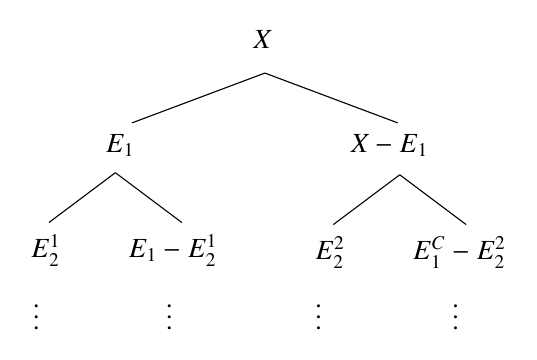
\begin{tikzpicture}[x=0.75pt,y=0.75pt,yscale=-1,xscale=1]
%uncomment if require: \path (0,476); %set diagram left start at 0, and has height of 476

%Straight Lines [id:da7156246342904542] 
\draw    (328,96) -- (264,120) ;
%Straight Lines [id:da871091531980348] 
\draw    (328,96) -- (392,120) ;
%Straight Lines [id:da22506695091814466] 
\draw    (256,144) -- (224,168) ;
%Straight Lines [id:da4242449719942467] 
\draw    (256,144) -- (288,168) ;
%Straight Lines [id:da7291448267881409] 
\draw    (393,145) -- (361,169) ;
%Straight Lines [id:da30881022603549657] 
\draw    (393,145) -- (425,169) ;

% Text Node
\draw (321,74.4) node [anchor=north west][inner sep=0.75pt]    {$X$};
% Text Node
\draw (250,124.4) node [anchor=north west][inner sep=0.75pt]    {$E_{1}$};
% Text Node
\draw (368,124.4) node [anchor=north west][inner sep=0.75pt]    {$X-E_{1}$};
% Text Node
\draw (214,172.4) node [anchor=north west][inner sep=0.75pt]    {$E_{2}^{1}$};
% Text Node
\draw (261,172.4) node [anchor=north west][inner sep=0.75pt]    {$E_{1} -E_{2}^{1}$};
% Text Node
\draw (351,173.4) node [anchor=north west][inner sep=0.75pt]    {$E_{2}^{2}$};
% Text Node
\draw (398,173.4) node [anchor=north west][inner sep=0.75pt]    {$E_{1}^{C} -E_{2}^{2}$};
% Text Node
\draw (215,198.4) node [anchor=north west][inner sep=0.75pt]    {$\vdots $};
% Text Node
\draw (279,198.4) node [anchor=north west][inner sep=0.75pt]    {$\vdots $};
% Text Node
\draw (351,198.4) node [anchor=north west][inner sep=0.75pt]    {$\vdots $};
% Text Node
\draw (417,198.4) node [anchor=north west][inner sep=0.75pt]    {$\vdots $};


\end{tikzpicture}
\end{center}
which forms an injection from $\mathfrak{M}$ to $2^\mathbb{Q}$, which is not countable.
\end{proof}
\begin{problem}\em
Prove an analogue of Theorem 1.1.6 for $n$ functions.
\end{problem}
\begin{proof}
We first state the Theorem of the condition $n$ functions:\par
\textbf{Theorem}. Let $u_1,u_2,\cdots,u_n$ be real measurable functions on a measurable space $X$. Let $\Phi$ be a continuous mapping of $\mathbb{R}^n$ into a topological space $Y$, and define 
$$h(x)=\Phi(u_1(x),u_2(x),\cdots,u_n(x))$$
for all $x\in X$. Then $h:X\to Y$ is measurable.\par
Let $f(x)=(u_1(x),u_2(x),\cdots,u_n(x))$. It suffices to show that $f$ is a measurable function. First, let $R$ be a cube in $\mathbb{R}^n$ which is the product of its segments $I_1,I_2,\cdots,I_n$. Then $f^{-1}\left( R \right) =\bigcup{f^{-1}\left( I_k \right)}$ is measurable. Now for an arbitrarily chosen $V\in\mathbb{R}^n$, let $V=\bigcup R_n$, where $R_n$ are cubes in $\mathbb{R}^n$, then 
$$
f^{-1}\left( V \right) =f^{-1}\left( \bigcup_{i=1}^{\infty}{R_n} \right) =\bigcup_{i=1}^{\infty}{f^{-1}\left( R_n \right)}=\bigcup_{i=1}^{\infty}{\bigcup_{j=1}^{\infty}{f^{-1}\left( I_{j}^{\left( i \right)} \right)}},
$$
which is measurable.
\end{proof}
\begin{problem}\em
Prove that if $f$ is a real function on a measurable space $X$ such that $\{x:f(x)\ge r\}$ is measurable for every rational $r$, then $f$ is measurable.
\end{problem}
\begin{proof}
Let $a$ be an arbitrarily chosen real number and $\{r_n\}$ be a rational sequence that converges to $a$. Therefore 
$$
\left\{ x:f\left( x \right) \ge a \right\} =\bigcap_{n=1}^{\infty}{\left\{ x:f\left( x \right) \ge r_n \right\}}
$$
is measurable since it is the intersection of countably many measurable sets.
\end{proof}
\begin{problem}\em
Let $\{a_n\}$ and $\{b_n\}$ be the sequences in $[-\infty,+\infty]$, and prove the following assertions:\par
(a)
$$\limsup_{n\to\infty}(-a_n)=-\liminf_{n\to\infty}a_n,$$
(b)
$$\limsup_{n\to\infty}(a_n+b_n)\le\limsup_{n\to\infty}a_n+\limsup_{n\to\infty}b_n$$
provided none of the sums is of the form $\infty-\infty$.\par
(c) If $a_n\le b_n$ for all $n$, then 
$$\liminf_{n\to\infty}a_n\le\liminf_{n\to\infty}b_n.$$
\end{problem}
\begin{proof}
(a) Let $c_n=\sup\{-a_n,-a_{n+1},-a_{n+2}\cdots\}$ and $\beta=\inf\{c_1,c_2,c_3,\cdots\}$, then 
$$\limsup_{n\to\infty}(-a_n)=\beta=-\sup\{-c_1,-c_2,-c_3,\cdots\}=-\liminf_{n\to\infty}a_n$$
since $-c_n=\inf\{a_n,a_{n+1},a_{n+2},\cdots\}$.\par
(b) It suffices to show that $\sup\{a_n+b_n\}\le\sup\{a_n\}+\sup\{b_n\}$. This follows from 
$$
\mathop {\mathrm{sup}} \limits_{n\in \mathbb{N} _+}\left( a_n+b_n \right) =\max_{n\in \mathbb{N} _+} \left\{ a_n+b_n \right\} \le \max_{n\in \mathbb{N} _+} \left\{ a_n+\max_{n\in \mathbb{N}} b_n \right\} =\max_{n\in \mathbb{N} _+} a_n+\max_{n\in \mathbb{N}} b_n.
$$\par
The equality clearly holds when $\{a_n\}$ and $\{b_n\}$ converges.
(c) This follows immediately from the fact that 
$$
\mathrm{inf}\left\{ a_n,a_{n+1},a_{n+2},\cdots \right\} \le \mathrm{inf}\left\{ b_n,b_{n+1},b_{n+2},\cdots \right\} .
$$
\end{proof}
\begin{problem}\em
(a) Suppose $f:X\to[-\infty,+\infty]$ and $g:X\to[-\infty,+\infty]$ are measurable. Prove that the sets 
$$\{x:f(x)<g(x)\},\{x:f(x)=g(x)\}$$
are measurable.\par
(b) Prove that the set of points at which a sequence of measurable real-valued functions converges (to a finite limit) is measurable.
\end{problem}
\begin{proof}
(a) This is clear since $f-g$ is measurable.\par
(b) Let $E$ be the set of $x$ such that $f_n(x)$ converges (to a finite limit). Since $f=\lim f_n=\limsup f_n$ is measurable by Theorem 1.1.11, we conclude that $E$ is measurable since $E=\bigcup_{n\ge 1}\{x:f(x)\le n\}$.
\end{proof}
\begin{problem}\em
Let $X$ be an uncountable set, let $\mathfrak{M}$ be the collection of all sets $E\subset X$ such that either $E$ or $E^c$ is at most countable, and define $\mu(E)=0$ in the first case, $\mu(E)=1$ in the last case. Prove that $\mathfrak{M}$ is a $\sigma$-algebra on $X$.
\end{problem}
\begin{proof}
We show by definition. Clearly $X\in\mathfrak{M}$ since $X^c=\emptyset$, which is at most countable. If $A\in\mathfrak{M}$, clearly $A^c\in\mathfrak{M}$ since either $A$ or $A^c$ is countable. Then suppose $A_1,A_2,\cdots\in\mathfrak{M}$. If there exists some $A_j$ is not countable, then $\bigcup A_n$ has a complement contained in $A_j^c$, which is at most countable. Otherwise $\bigcup A_n$ is at most countable. Therefore $\mathfrak{M}$ is a $\sigma$-algebra.
\end{proof}
\begin{problem}\em
Suppose $f_n:X\to [0,+\infty]$ is measurable for $n=1,2,\cdots$ and $f_1\ge f_2\ge\cdots\ge 0$, $f_n(x)\to f(x)$ as $n\to\infty$ for all $x\in X$. If $f_1\in L^1(\mu)$, then 
$$\lim_{n\to\infty}\int_Xf_n\mathrm{d}\mu=\int_Xf\mathrm{d}\mu.$$
Show that this conclusion is false if $f_1\in L^1(\mu)$ is omitted.
\end{problem}
\begin{proof}
If $\int f_1<\infty$, then by $|f_n(x)|\le f_1(x)$ and the Dominated Convergent Theorem we have 
$$\lim_{n\to\infty}\int_Xf_n\mathrm{d}\mu=\int_Xf\mathrm{d}\mu.$$
If $\int f_1=\infty$, then since $f_1\ge 0$, we have $\int|f_1|=\infty$, which contradict to the fact that $f_1\in L^1(\mu)$.\par
Now if the condition $f_1\in L^1(\mu)$ is omitted, let $f_n=\frac{1}{n}$, then $f\equiv 0$ and hence $\int f=0$. However $\int f_n=\infty$ for all $n\in\mathbb{N}_+$.
\end{proof}
\begin{problem}\em
Give an example that the inequality may strictly holds in Fatou's Lemma.
\end{problem}
\begin{proof}
Let 
$$
f_n=\begin{cases}
	0,x\in \left\{ 0 \right\} \cup \left[ \frac{1}{n},1 \right] ,\\
	1,x\in \left( 0,\frac{1}{n} \right) ,\\
\end{cases}
$$
then 
$$
0=\int_{\left[ 0,1 \right]}{\left( \lim_{n\rightarrow \infty} f_n \right) \mathrm{d}x}<\lim_{n\rightarrow \infty} \int_{\left[ 0,1 \right]}{f_n\mathrm{d}x}=1
$$
is a desired example.
\end{proof}
\begin{problem}\em
Suppose $\mu$ is a positive measure on $X$, $f:X\to [0,+\infty]$ is measurable, $\int_Xf=c$, where $c\in (0,+\infty)$. Let $\alpha$ be a constant, show that 
$$
\lim_{n\rightarrow \infty} \int_X{n\log \left[ 1+\left( \frac{f}{n} \right) ^{\alpha} \right] \mathrm{d}\mu}=\begin{cases}
	\infty ,0<\alpha <1;\\
	c,\alpha =1;\\
	0,1<\alpha <\infty .\\
\end{cases}
$$
\end{problem}
\begin{proof}
If $\alpha=1$, we have $n\log \left( 1+\frac{f}{n} \right) \le f$ and hence the integrand is dominated by $f$. Therefore by Dominated Convergence Theorem we have 
$$
\lim_{n\rightarrow \infty} \int_X{n\log \left( 1+\frac{f}{n} \right) \mathrm{d}\mu}=\int_X{\lim_{n\rightarrow \infty} n\log \left( 1+\frac{f}{n} \right) \mathrm{d}\mu}=\int_X{f\mathrm{d}\mu}=c.
$$
Similarly it is easy to see that the integrand is dominated by $\alpha f$ for $\alpha>1$, therefore 
$$
\lim_{n\rightarrow \infty} \int_X{n\log \left[ 1+\left( \frac{f}{n} \right) ^{\alpha} \right] \mathrm{d}\mu}=\int_X{\left( \lim_{n\rightarrow \infty} n\log \left[ 1+\left( \frac{f}{n} \right) ^{\alpha} \right] \right) \mathrm{d}\mu}=0.
$$
Now suppose $0<\alpha<1$. By Fatou's Lemma, we have 
$$\liminf_{n\to\infty}\int_Xn\log\left[1+\left(\frac{f}{n}\right)^\alpha\right]\mathrm{d}\mu\ge\int_X\left(\liminf_{n\to\infty}n\log\left[1+\left(\frac{f}{n}\right)^\alpha\right]\right)\mathrm{d}\mu=\infty,$$
hence the limit of the integral is $\infty$.
\end{proof}
\begin{problem}\em
Suppose $\mu(X)<\infty$, $\{f_n\}$ is a sequence of bounded complex measurable functions on $X$, and $f_n\to f$ uniformly on $X$. Prove that 
$$
\lim_{n\rightarrow \infty} \int_X{f_n\mathrm{d}\mu}=\int_X{f\mathrm{d}\mu}.
$$
Show that the hypothesis is not true if $\mu(X)<\infty$ is omitted.
\end{problem}
\begin{proof}
Since the convergence is uniform, we may find an $N$ such that $|f_n(x)-f(x)|\le 1$ for all $n>N$. Let $C=\max\{|f(x)+1|,|f(x)-1|\}$ and $C^\prime=\{|f_1(x)|,|f_2(x)|,\cdots,|f_N(x)|\}$ and $M=\max\{C,C^\prime\}$, then $|f_n(x)|\le M$ for all $x\in X$ and $n\in\mathbb{N}$. Since $\mu(X)<\infty$ we have $\int_XM=M\mu(X)<\infty$, therefore $M\in L^1(\mu)$. Hence by the Dominated Convergence Theorem we have 
$$
\lim_{n\rightarrow \infty} \int_X{f_n\mathrm{d}\mu}=\int_X{f\mathrm{d}\mu}.
$$
Now if $\mu(X)=\infty$, see Exercise 1.7.7.
\end{proof}
\begin{problem}\em
Show that $A=\bigcap_{n=1}^\infty\bigcup_{k=n}^\infty E_k$ in Theorem 1.6.5, and hence prove the theorem without any reference to integration.
\end{problem}
\begin{proof}
Since $x\in A$ implies $x$ lies in infinitely many $E_k$'s, therefore for all $n\in\mathbb{N}_+$, there exists $k\in\mathbb{N}_+$, such that $x\in E_k$ for some $k\ge n$ or otherwise there are only $n$ possible $E_k$'s that $x$ lies in. By interpreting such condition into the language of sets we have 
$$A=\bigcap_{n=1}^\infty\bigcup_{k=n}^\infty E_k.$$
Now denote $B_n=\bigcup_{k\ge n}E_k$, hence $\mu(B_1)<\infty$, $B_1\subset B_2\subset\cdots\subset B_n\subset\cdots$, and $\mu(B_n)\to\mu(A)$. Since $\mu(B_n)\le\sum_{k\ge n}\mu(E_k)$, we have $\mu(B_n)\to 0$ as $n\to\infty$, and hence $\mu(A)=0$.
\end{proof}
\begin{problem}\em
Suppose $f\in L^1(\mu)$. Prove that to each $\varepsilon>0$, there exits a $\delta>0$ such that $\int_E|f|\mathrm{d}\mu<\varepsilon$ whenever $\mu(E)<\delta$.
\end{problem}
\begin{proof}
We begin by choosing a large $A\subset X$ such that 
$$
\int_X{\left( \left| f \right|-\left| \chi _A\cdot f \right| \right) \mathrm{d}\mu}<\frac{\varepsilon}{2}.
$$
Since $f\in L^1(\mu)$ we may suppose $|\chi_Af|\le M$. Now let $\delta=\frac{\varepsilon}{2M}$, we have 
$$
\int_E{\left| f \right|\mathrm{d}\mu}=\int_E{\left( \left| f \right|-\left| \chi _A\cdot f \right| \right) \mathrm{d}\mu}+\int_E{\left| \chi _A\cdot f \right|\mathrm{d}\mu}\le \frac{\varepsilon}{2}+M\mu \left( E \right) <\frac{\varepsilon}{2}+\frac{\varepsilon}{2}=\varepsilon ,
$$
which finished our proof.
\end{proof}
\begin{problem}\em
Show that $\int cf=c\int f$ is true when $c=\infty$.
\end{problem}
\begin{proof}
If $f\equiv 0$, then $cf\equiv 0$, and the left side equals to $0$. On the other hand, since $f\equiv 0$ we have $\int f=0$, hence $c\int f=0$, and the equality holds since $0=0$. The condition is similar if $\mu(X)=0$, where $\int_Xf$ is considered. Otherwise $\int cf=c\int f=\infty$, the equality still holds since $\infty=\infty$.
\end{proof}
\newpage
\section{Positive Borel Measures}
\subsection{Vector Spaces}
A \textbf{complex vector space}, or a vector space over the complex field $\mathbb{C}$, is a set $V$ whose elements are called \textbf{vectors} and in which two operations, called \textbf{addition} and \textbf{scalar multiplication}, are defined with the following algebraic properties:\par
(a) To every pair of vectors $x$ and $y$ there corresponds a vector $x+y$, in such a way that $x+y=y+x$ and $x+(y+z)=(x+y)+z$.\par
(b) $V$ contains a unique vector $0$, called the \textbf{zero vector} or \textbf{origin} of $V$, such that $x+0=x$ for all $x\in V$.\par
(c) For every $x\in V$ there corresponds a unique vector $-x$ such that $x+(-x)=0$.\par
(d) To each pair $(\alpha,x)$, where $x\in V$ $\alpha\in\mathbb{C}$ is called a \textbf{scalar}, there is associated a vector $\alpha x\in V$, in such a way that $1x=x$, $\alpha(\beta x)=(\alpha \beta)x$, and the two distributive laws:
$$\alpha(x+y)=\alpha x+\alpha y;\hspace{0.5cm}(\alpha+\beta)x=\alpha x+\beta x.$$
A \textbf{linear transformation} of a vector space $V$ into a vector space $V_1$ is a mapping $\Lambda$ of $V$ into $V_1$ such that 
$$\Lambda(\alpha x+\beta y)=\alpha\Lambda x+\beta\Lambda y$$
for all $x,y\in V$ and $\alpha,\beta\in\mathbb{C}$. In the special case in which $V_1$ is the field of scalars, then $\Lambda$ is called a \textbf{linear functional}.\par
We now see integration as a linear functional. For instance, by Theorem 1.5.3 we know that $L^1(\mu)$ is a vector space, and the mapping $f\mapsto\int_X f$ is a linear functional. Similarly, if $g$ is a bounded measurable function, the mapping $f\mapsto\int_Xfg$ is a linear functional on $L^1(\mu)$. We shall see in Chapter 6 that the second functional is, in a sense, the only interesting ones on $L^1(\mu)$.\par
For another example, let $C$ be the vector space of all continuous functions on the unit interval $I=[0,1]$. Let 
$$\Lambda x=\int_0^1f(x)\mathrm{d}x,f\in C,$$
where the integral is the original Riemann integral, then $\Lambda$ is a linear functional on $C$. $\Lambda$ has another property: it is a positive functional, that is, $\Lambda f\ge 0$ whenever $f\ge 0$.\par
One of the task that still ahead of us is the construction of the Lebesgue measure. The construction can be based on the linear functional above, by the following observation: Consider a segment $(a,b)\subset I$, and consider the class of all $f\in C$, which satisfies $0\le f\le 1$ and $f(x)=0$ for all $x\notin(a,b)$. Clearly $\Lambda f<b-a$ for all such $f$, but we can choose $f$ so that $\Lambda f$ is as close to $b-a$ as desired. Thus the length (or measure) of $(a,b)$ is intimately related to the values of the functional $\Lambda$.\par
The preceding observation, when looked at from a more general point of view, leads to a remarkable and extremely important theorem of F.Riesz:
\begin{theorem}
To every positive linear functional $\Lambda$ on $C$ corresponds a finite positive Borel measure $\mu$ on $I$ such that 
$$\Lambda f=\int_If\mathrm{d}\mu,f\in C.$$
\end{theorem}
We will proof this theorem in a more general sense in Section 2.3. The converse is obvious. If $\mu$ is a positive Borel measure on $I$ and $\Lambda$ is defined above, then $\Lambda$ is a positive linear functional on $C$. Note that the proof of this Theorem can easily be established on $\mathbb{R}^n$. Actually the proof of this theorem has nothing to do with the Euclidean properties of $\mathbb{R}^n$ but topological properties.
\subsection{Topological Preliminaries}
We first give some basic definitions.
\begin{definition}
Let $X$ be a topological space.\par
(a) A set $E\subset X$ is \textbf{closed} if its complement is open.\par
(b) The \textbf{closure} $\overline{E}$ of a set $E\subset X$ is the smallest closed set in $X$ which contains $E$.\par
(c) A set $K\subset X$ is \textbf{compact}, if every open cover of $K$ contains a finite subcover.\par
(d) A \textbf{neighborhood} of a point $p\in X$ is any open subset of $X$ which contains $p$.\par
(e) $X$ is a \textbf{Hausdorff space} if the following is true: If $p\in X,q\in X$ and $p\ne q$, then $p$ has a neighborhood $U$ and $q$ has a neighborhood $V$ such that $U\cap V=\emptyset$.\par
(f) $X$ is \textbf{locally compact} if every point of $X$ has a neighborhood whose closure is compact.
\end{definition}
\begin{note}\em
Here are some comments on Definition 2.2.1.\par
(a) $\emptyset$ and $X$ are both open and closed, since the complement of one is another. By De Morgan's law it is easy to show that finite unions of closed sets are closed, and arbitrary intersections of closed sets are closed.\par
(b) We show the existence of $\overline{E}$. Let $\Omega$ be the collection of all closed sets that contains $E$, then $\bigcap_{A\in\Omega}A$ is the desired closure. $\Omega$ is not empty since $X\in\Omega$.\par
(c) We state in a more explicit way: If $\{V_\alpha\}$ is an open cover of $E$, that is, $V_\alpha$ is open and $E\subset\bigcup V_\alpha$, then there exists finite many $V_\alpha$'s, denote as $V_1,V_2,\cdots,V_n$, such that $E\subset\bigcup_{i=1}^nV_i$.\par
(e) Every metric space is a Hausdorff space. In particular $\mathbb{R}^n$ is a Hausdorff space.\par
(f) Obviously every compact space is locally compact. Also note that $\mathbb{R}^n$ is locally compact, since the closure if compact for all subsets of $\mathbb{R}^n$ by Heine-Borel Theorem.
\end{note}
\begin{theorem}
Suppose $K$ is compact and $F$ is closed, in a topological space $X$. If $F\subset K$, then $F$ is compact.
\end{theorem}
\begin{proof}
Let $\{V_\alpha\}$ be an open cover of $F$ and $W=K^c$. Then $W\cup\bigcup_{\alpha}V_\alpha$ is a cover of $X$. Since $K$ is compact, there are finitely many $\{V_i\}$ such that $K\subset W\cup \left( \bigcup{V_i} \right) $, and therefore $\bigcup V_i$ is a finite subcover of $F$, therefore $F$ is compact.
\end{proof}
\begin{corollary}
If $A\subset B$ and $B$ has compact closure, so does $A$.
\end{corollary}
\begin{proof}
It suffices to observe that $\overline{A}\subset\overline{B}$, and apply Theorem 2.2.2.
\end{proof}
\begin{theorem}
Suppose $X$ is a Hausdorff space, $K\subset X$, $K$ is compact, and $p\in K^c$. Then there are open sets $U$ and $W$ such that $p\in U$, $K\subset W$, and $U\cap W=\emptyset$.
\end{theorem}
\begin{proof}
Let $q\in K$, then since $X$ is a Hausdorff space, there exists $U_q$ and $V_q$ such that $p\in U_q$, and $U_q\cap V_q=\emptyset$. Since $K$ is compact, we may select some $p_1,p_2,\cdots,p_n\in K$ such that 
$$K\subset V_{q_1}\cup V_{q_2}\cup\cdots\cup V_{q_n}.$$
Therefore let 
$$U=U_{q_1}\cap U_{q_2}\cap\cdots\cap U_{q_n},W=V_{q_1}\cup V_{q_2}\cup\cdots\cup V_{q_n},$$
we get desired $U$ and $W$.
\end{proof}
\begin{corollary}
(a) Compact subsets of Hausdorff spaces are closed.\par
(b) If $F$ is closed and $K$ is compact in a Hausdorff space, then $F\cap K$ is compact.
\end{corollary}
\begin{proof}
(a) By Theorem 2.2.4 we know that for all $x\in K^c$ there exists an open set $U$ such that $x\in U$ and $U\cap K=\emptyset$. Therefore $K^c$ is open.\par
(b) Since $K$ is compact in a Hausdorff space, $K$ is closed. Therefore $K\cap F\subset K$ is closed. Then apply Theorem 2.2.2.
\end{proof}
\begin{theorem}
If $\{K_\alpha\}$ is a collection of compact subsets of a Hausdorff space and if $\bigcap_\alpha K_\alpha=\emptyset$, then some finite subcollection of $\{K_\alpha\}$ also has empty intersection.
\end{theorem}
\begin{proof}
Since $K_\alpha$ is compact in a Hausdorff space, $K_\alpha$ is closed. Then let $V_\alpha=K_\alpha^c$. Fix $K_1$, since $\bigcap K_\alpha=\emptyset$, then no $x\in K_1$ lies in all $K_\alpha$'s, therefore $\{V_\alpha\}$ is an open cover of $K_1$. Since $K_1$ is compact, there are finite many $V_i$'s such that $K_1\subset\bigcup_{i=1}^n V_i$, therefore $K_1\cap\bigcap_{i=1}^nV_i^c=\emptyset$.
\end{proof}
\begin{theorem}
Suppose $U$ is open in a locally compact Hausdorff space $X$, $K\subset U$, $K$ is compact, then there is an open set $V$ with compact closure such that 
$$K\subset V\subset\overline{V}\subset U.$$
\end{theorem}
\begin{proof}
Since every point of $K$ has a neighborhood with compact closure, and since $K$ is covered by the union of finitely many of these neighborhoods, $K$ lies in an open set $G$ with compact closure. If $U=X$, then take $V=G$. Otherwise let $C$ be the complement of $U$. By Theorem 2.24 we know that there exists an open set $W_p$ for each $p\in C$ such that $K\subset W_p$ and $p\notin\overline{W_p}$. Hence $\{C\cap\overline{G}\cap\overline{W_p}\}_{p\in C}$ is a collection of compact sets with empty intersection. By Theorem 2.2.6 there are finite many points $p_1,p_2,\cdots,p_n$ such that 
$$
C\cap \overline{G}\cap \overline{W_{p_1}}\cap \overline{W_{p_2}}\cap \cdots \cap \overline{W_{p_n}}=\emptyset .
$$
Therefore let 
$$
V=G\cap W_{p_1}\cap W_{p_2}\cap \cdots \cap W_{p_n},
$$
then $V$ has the required properties.
\end{proof}
\begin{definition}
Let $f$ be a real (or extended-real) function on a topological space.\par
If
$$\{x:f(x)>\alpha\}$$
is open for every real $\alpha$, then $f$ is said to be \textbf{lower semicontinuous}.\par
If 
$$\{x:f(x)<\alpha\}$$
is open for every real $\alpha$, then $f$ is said to be \textbf{upper semicontinuous}.
\end{definition}
A real function is continuous if and only if it is both upper and lower semicontinuous. The simplest examples of semicontimuity are furnished by characteristic functions:\par
Characteristic functions of open [resp. closed] sets are lower [resp. upper] semicontinuous.\par
The following property is an immediate consequence of the definitions:
\begin{proposition}
The supremum [resp. infimum] of any collection of lower [resp. upper] semicontinuous functions is lower [resp. upper] continuous.
\end{proposition}
\begin{proof}
We show that the supremum of any collection of lower semicontinuous functions is lower continuous. Let $\{f_n\}$ be a class of lower semicontinuous functions, then 
$$
\left\{ x:\mathop {\mathrm{sup}} \limits_{n}f_n\left( x \right) >\alpha \right\} =\bigcup_n{\left\{ x:f_n\left( x \right) >\alpha \right\}}
$$
is the union of some open sets, which is open. Therefore $\sup_nf_n$ is lower semicontinuous.
\end{proof}
\begin{definition}
The \textbf{support} of a complex function $f$ on a topological space $X$ is the closure of the set $\{x:f(x)\ne 0\}$. The collection of all continuous complex functions on $X$ whose support is compact is denoted by $C_c(X)$.
\end{definition}
By definition we know that $C_c(X)$ is a vector space, since the support of $f+g$ lies in the union of the support of compact sets, which is compact, and the sum of two continuous complex functions is continuous, as are scalar multiples of continuous functions.
\begin{theorem}
Let $X$ and $Y$ be topological spaces, and let $f:X\to Y$ be continuous. If $K$ is a compact subset of $X$, then $f(K)$ is compact.
\end{theorem}
\begin{proof}
Let $\{V_\alpha\}$ be an open cover of $f(K)$, then $\{f^{-1}(V_\alpha)\}$ is an open cover of $K$. Since $K$ is compact, we have the finite subcover $\{f^{-1}(V_i)\}$, whence $K\subset\bigcup f^{-1}(V_i)$. Therefore $f(K)\subset\bigcup V_i$ has a finite subcover, therefore compact.
\end{proof}
An immediate consequence of this Theorem is as follows:
\begin{corollary}
The range of any $f\in C_c(X)$ is a compact subset of the complex plane.
\end{corollary}
The proof of this corollary is easy by applying Theorem 2.2.11 to $f$.\par
We introduce some notations that will be used throughout this chapter. We write $K\prec f$ if $K$ is a compact subset of $X$, that $f\in C_c(X)$, that $0\le f\le 1$ for all $x\in X$, and that $f(x)=1$ for all $x\in K$. The notation $f\prec V$ will mean that $V$ is open, that $f\in C_c(X)$, $0\le f\le 1$ and the support of $f$ lies in $V$. The notation $K\prec f\prec V$ will be used when $K\prec f$ and $f\prec V$ are both hold.\par
\begin{theorem}(Urysorn's Lemma)
Suppose $X$ is a locally compact Hausdorff space, $V$ is open in $X$, $K\subset V$ and $K$ is compact. Then there exists an $f\in C_c(X)$, such that $K\prec f\prec V$.
\end{theorem}
In terms of characteristic functions, the conclusion asserts the existence of a \textit{continuous function} $f$ which satisfies $\chi_K\le f\chi_V$. Note that it is easy to find semicontinuous functions which do this: $\chi_k$ and $\chi_V$, for instance.
\begin{proof}
Let $r_1=0,r_2=1$ and let $\{r_n\}$ be an enumeration of the rationals in $[0,1]$. By Theorem 2.2.7 we may find open sets $V_0$ and $V_1$ such that $\overline{V_0}$ is compact and 
$$
K\subset V_1\subset \overline{V_1}\subset V_0\subset \overline{V_0}\subset V.
$$
Suppose $n\ge 2$ and $V_{r_1},\cdots,V_{r_n}$ have been chosen in such a manner that $r_i<r_j$ implies $\overline{V_{r_j}}\subset\overline{V_{r_i}}$. Then one of the numbers $r_i\in\{r_1,\cdots,r_n\}$ is the largest one which is smaller than $r_{n+1}$, also there is $r_j\in\{r_1,\cdots,r_n\}$  be the smallest one which is larger than $r_{n+1}$. Then by Theorem 2.2.7 we may find $V_{r_i}$ and $V_{r_j}$ that is open with compact closure such that 
$$
\overline{V_{r_i}}\subset V_{r_{n+1}}\subset \overline{V_{r_{n+1}}}\subset V_{r_j}.
$$
Therefore we defined inductively a sequence of $\{V_{r}\}_{r\in\mathbb{Q}\cap[0,1]}$ such that satisfies the following properties: $K\subset V_1$, $\overline{V_0}\subset V$, each $\overline{V_r}$ is compact and $s>r$ implies $\overline{V_s}\subset V_r$. Define 
$$
f_r\left( x \right) =\begin{cases}
	r,x\in V_r;\\
	0,\mathrm{otherwise},\\
\end{cases}\hspace{0.5cm}g_s\left( x \right) =\begin{cases}
	1,x\in \overline{V_s};\\
	s,\mathrm{otherwise},\\
\end{cases}
$$
and 
$$
f=\mathop {\mathrm{sup}} \limits_{r}f_r,\hspace{0.5cm}g=\mathop {\mathrm{inf}} \limits_{s}g_s,
$$
then $f$ is lower semicontinuous and $g$ is upper semicontinuous. It's clear to see that $0\le f\le 1$ and has a support in $\overline{V_0}$. It suffices to show that $f=g$. Now if $f_r(x)>g_s(x)$ for some $r,s$, we have $r>s$, $x\in V_r$ and $x\notin\overline{V_s}$. However this cannot be true since $r>s$ implies $V_r\subset V_s$. Hence $f\le g$. Now if $f<g$, let $s,r$ be rationals such that  $f(x)<r<s<g(x)$, then since $f(x)<r$, we have $x\notin V_r$, also since $g(x)>s$, we have $x\in\overline{V_s}$. However since $r<s$ we have $V_s\subset V_r$, which is impossible. Therefore $f=g$ and we finished our proof.
\end{proof}
\begin{theorem}
Suppose $V_1,V_2,\cdots,V_n$ are open subsets of a locally compact Hausdorff space $X$, $K$ is compact and $K\subset\bigcup V_i$. Then there exists functions $h_i\prec V_i$ for all $i=1,2,\cdots,n$ such that $\sum h_i(x)=1$ for all $x\in K$.
\end{theorem}
\begin{proof}
By Theorem 2.2.7, we may find a neighborhood $W_{x}$ for each $x\in K$ with compact closure such that $\overline{W_x}\subset V_i$ for some $i$. Since $K$ is compact, there are finitely many $W_{x_1},W_{x_2},\cdots,W_{x_n}$ such that 
$$
K\subset W_{x_1}\cup W_{x_2}\cup \cdots \cup W_{x_m}.
$$
If $1\le i\le n$, let $H_i$ be the union of those $\overline{W_{x_j}}$ which lie in $V_i$. By Urysorn's Lemma, there are functions $H_i\prec g_i\prec V_i$. Define $h_1=g_1$ and $h_i=(1-g_1)(1-g_2)\cdots(1-g_{i-1})g_i$, then $h_i\prec V_i$. Since 
$$
K\subset H_1\cup H_2\cup \cdots \cup H_n,
$$
for each $x\in K$ there is at least one $i$ such that $x\in H_i$, hence $g_i(x)=1$. Therefore 
$$\sum_{i=1}^nh_i(x)=1-\prod_{i=1}^n(1-g_i(x))=1,$$
and we finished our proof.
\end{proof}
\begin{note}\em
The collection $\{h_1,h_2,\cdots,h_n\}$ is called a \textbf{partition of unity on $K$}, subordinate to the cover $\{V_1,V_2,\cdots,V_n\}$.
\end{note}
\subsection{The Riesz Representation Theorem (Real Version)}
We will use the content of this section to prove this profound theorem:
\begin{theorem}(Riesz)
Let $X$ be a locally compact Hausdorff space, and let $\Lambda$ be a positive linear functional on $C_c(X)$. Then there exists a $\sigma$-algebra $\mathfrak{M}$ in $X$ which contains all Borel sets in $X$, and there exists a unique positive measure $\mu$ on $\mathfrak{M}$ which represents $\Lambda$ in the sense that \par
(a) $\Lambda f=\int_Xf\mathrm{d}\mu$ for every $f\in C_c(X)$\par
and with the following properties:\par
(b) $\mu(K)<\infty$ for every compact set $K\subset X$;\par
(c) For every $E\in\mathfrak{M}$, we have 
$$\mu(E)=\inf\{\mu(V):E\subset V, V\ \text{open}\}.$$\par
(d) The relation 
$$\mu(E)=\sup\{\mu(K):K\subset E, K\ \text{compact}\}$$
holds for every open set $E$, and for every $E\in\mathfrak{M}$ with $\mu(E)<\infty$.\par
(e) If $E\in\mathfrak{M}$, $A\subset E$ and $\mu(E)=0$, then $A\in\mathfrak{M}$.
\end{theorem}
\begin{note}\em
For the sake of clarity, we explain the term "positive linear function". Let $f\in C_c(X)$ and $f(X)\in[0,+\infty)$, then $\Lambda f\in[0,+\infty)$.
\end{note}
\begin{proof}
We proof the Theorem by 13 steps.\par
\textbf{Step}.1: We show that $\mu$ is unique. Let $\mu_1,\mu_2$ be measures that satisfies the properties in Theorem 2.3.1, then it suffices to show that for each compact set $K\subset X$ we have $\mu_1(K)=\mu_2(K)$ by (d). By (b) we know that $\mu_1(K)<\infty$, therefore for an arbitrary $\varepsilon>0$ by (c) there exists an open set $V$ such that $K\subset V$ and $\mu_2(V)<\mu_2(K)+\varepsilon$. By Urysorn's Lemma there exists $f$ such that $K\prec f\prec V$. Hence 
$$
\mu _1\left( K \right) =\int_X{\chi _K\mathrm{d}\mu}\le \int_X{f\mathrm{d}\mu}=\Lambda f=\int_X{f\mathrm{d}\mu _2}\le \int_X{\chi _V\mathrm{d}\mu _2}=\mu _2\left( V \right) <\mu _2\left( K \right) +\varepsilon ,
$$
whence $\mu_1(K)\le\mu_2(K)$. By interchanging the position of $\mu_1$ and $\mu_2$ we get $\mu_2(K)\le\mu_1(K)$, hence $\mu_1(K)=\mu_2(K)$.\par
\textbf{Step}.2: Construction of $\mu$ and $\mathfrak{M}$. For every open set $V\subset X$, define $\mu(V)=\sup\{\Lambda f:f\prec V\}$. Clearly for open sets $V_1\subset V_2$ we have $\mu(V_1)\le\mu(V_2)$, therefore 
$$\mu(E)=\sup\{\mu(V):E\subset V,V\ \text{open}\}$$
for all $E$ that is open. Now we define 
$$\mu(E)=\sup\{\mu(V):E\subset V,V\ \text{open}\}$$
for all $E\subset X$. Let $\mathfrak{M}_F$ be the class of all $E\subset X$ such that $\mu(E)<\infty$, and 
$$\mu(E)=\inf\{\mu(K):K\subset E,K\ \text{compact}\}.$$
Then we define $\mathfrak{M}$ be the class of all $E\subset X$ such that for all compact $K\subset X$, $E\cap K\in\mathfrak{M}_F$.\par
Now we show that the $\mu$ and $\mathfrak{M}$ defined above have the desired properties in Theorem 2.3.1.\par
\textbf{Step}.3: Some trivial observations. By the definition of $\mu$ we know that (c) holds. Also (e) holds, since it is clear that $\mu$ is monotonic and $\mu(E)=0$ implies $E\in\mathfrak{M}_F$ and $E\in\mathfrak{M}$.\par
Since the proof of the rest properties are rather long, we break them into several steps.\par
\textbf{Step}.4: If $E_1,E_2,E_3,\cdots$ are arbitrary subsets of $X$, then 
$$\mu\left(\bigcup_{i=1}^\infty E_i\right)\le\sum_{i=1}^\infty\mu(E_i).$$
We first show that $\mu(V_1\cup V_2)\le\mu(V_1)+\mu(V_2)$ for open sets $V_1,V_2$. Choose $g\prec V_1\cup V_2$. Then by Theorem 2.2.14 there exists $h_i\prec V_i$ such that $h_1+h_2=1$ for all $x$ on the support of $g$. Therefore 
$$
\Lambda g=\Lambda \left( h_1g \right) +\Lambda \left( h_2g \right) \le \mu \left( V_1 \right) +\mu \left( V_2 \right) ,
$$
and we finished our proof. Now suppose $\mu(E_i)=\infty$ for some $i$, then the subadditivity clearly holds. So we suppose $\mu(E_i)<\infty$ for all $i$. Therefore by the definition of $\mu$, for all $\varepsilon>0$ we may choose an open set $V_i$ such that $\mu(V_i)<\mu(E_i)+\frac{\varepsilon}{2^i}$. Let $V=\bigcup V_i$ and $f\prec V$, since $f$ has a compact support, there exists some $n$ such that $f\prec V_1\cup\cdots\cup V_n$. Hence 
$$
\Lambda f\le \mu \left( V_1\cup \cdots \cup V_n \right) \le \mu \left( V_1 \right) +\mu \left( V_2 \right) +\cdots +\mu \left( V_n \right) \le \sum_{i=1}^{\infty}{\mu \left( V_i \right)}+\varepsilon .
$$
Since this is true for all $f\prec V$, and $\bigcup{E_i}\subset V$, we proved that 
$$
\mu \left( \bigcup_{i=1}^{\infty}{E_i} \right) \le \mu \left( V \right) \le \sum_{i=1}^{\infty}{\mu \left( E_i \right)}+\varepsilon ,
$$
let $\varepsilon\to 0$.\par
\textbf{Step}.5: If $K$ is compact, then $K\in\mathfrak{M}_F$, and 
$$\mu(K)=\inf\{\Lambda f:K\prec f\}.$$
Let $K\prec f$, and $0<\alpha<1$, let $V_\alpha=\{x:f(x)>\alpha\}$, then $K\subset V_\alpha$, and $\alpha g\le f$ whenever $g\prec V_\alpha$. Hence 
$$
\mu \left( K \right) \le \mu \left( V_{\alpha} \right) =\mathrm{sup}\left\{ \Lambda g:g\prec V_{\alpha} \right\} \le \frac{1}{\alpha}\Lambda f.
$$
Let $\alpha\to 1$, we conclude that $\mu(K)\le\Lambda f$. Thus $\mu(K)<\infty$. Since $K$ evidently satisfies the condition $\mu(K)=\sup\{\mu(C):C\subset K,C\ \text{compact}\}$, we have $K\in\mathfrak{M}_F$. If $\varepsilon>0$, by the definition of $\mu$ we nay choose an open set $V\supset K$ such that $\mu(V)<\mu(K)+\varepsilon$, therefore by Urysorn's Lemma we have $K\prec f\prec V$, and hence 
$$
\Lambda f\le \mu \left( V \right) <\mu \left( K \right) +\varepsilon ,
$$
the proof is finished combining the inequality above and $\mu(K)<\Lambda f$.\par
\textbf{Step}.6: Every open set satisfies the condition 
$$\mu(V)=\sup\{\mu(K):K\subset V,K\ \text{compact}\}.$$
Hence $\mathfrak{M}_F$ contains every open set $V$ with $\mu(V)<\infty$. Let $\alpha$ be a real number such that $\alpha<\mu(V)$, it suffices to show that there exists a compact $K\subset V$ such that $\alpha<\mu(K)$. Let $f\prec V$ with $\alpha<\Lambda f$. If $W$ is an open set which contains the support $K$ of $f$, then $f\prec W$, and $\Lambda f\le\mu(W)$, thus $\Lambda f\le\mu(K)$. Therefore $K$ is a subset of $V$ and satisfies $\alpha<\mu(K)$ and we finished our proof.\par
\textbf{Step}.7:Suppose $E=\bigcup_{i=1}^\infty E_i$, where $E_i$ are disjoint elements of $\mathfrak{M}_F$, then 
$$
\mu \left( E \right) =\sum_{i=1}^{\infty}{\mu \left( E_i \right)}.
$$
If $\mu(E)<\infty$, then also $E\in\mathfrak{M}_F$. We first show that for compact $K_1$ and $K_2$ that are disjoint, we have 
$$
\mu \left( K_1\cup K_2 \right)=\mu \left( K_1 \right) +\mu \left( K_2 \right) .
$$
Choose $\varepsilon>0$. By Urysorn's Lemma, there exists $f\in C_c(X)$ such that $f(x)=1$ for $x\in K_1$, $f(x)=0$ for $x\in K_2$, and $0\le f\le 1$. By Step 5 we have $g$ such that $K_1\cup K_2\prec g$ and $\Lambda g<\mu \left( K_1\cup K_2 \right) +\varepsilon $. Note that $K_1\prec fg$ and $K_2\prec (1-f)g$, therefore 
$$
\mu \left( K_1 \right) +\mu \left( K_2 \right) \le \Lambda \left( fg \right) +\Lambda \left( g-fg \right) =\Lambda g<\mu \left( K_1\cup K_2 \right) +\varepsilon ,
$$
hence
$$
\mu \left( K_1 \right) +\mu \left( K_2 \right) \le \mu \left( K_1\cup K_2 \right) .
$$
We have shown in previous steps that 
$$
\mu \left( K_1 \right) +\mu \left( K_2 \right) \ge \mu \left( K_1\cup K_2 \right) ,
$$
and we finished the proof. Now if $\mu(E_i)=\infty$, the equality $\infty=\infty$ clearly holds. Let $\mu(E_i)<\infty$ for all $i$. Therefore for an arbitrarily chosen $\varepsilon>0$, there exists some compact $K_i\subset E_i$ satisfies $\mu \left( K_i \right) >\mu \left( E_i \right) -\frac{\varepsilon}{2^i}$. Therefore let $H_n=K_1\cup K_2\cup\cdots\cup K_n$, we have 
$$
\mu \left( E \right) \ge \mu \left( H_n \right) =\sum_{i=1}^n{\mu \left( K_i \right)}>\sum_{i=1}^n{\mu \left( E_i \right)}-\varepsilon .
$$
Letting $n\to\infty$, we have 
$$
\mu \left( E \right) =\sum_{i=1}^{\infty}{\mu \left( E_i \right)}.
$$
Now if $\mu(E)<\infty$, we have 
$$
\mu \left( E \right) \le \sum_{i=1}^N{\mu \left( E_i \right)}+\varepsilon 
$$
for some $N$, therefore $\mu(E)\le\mu(H_n)+2\varepsilon$, and this shows that $E\in\mathfrak{M}_F$.\par
\textbf{Step}.8: If $E\in\mathfrak{M}_F$ and $\varepsilon>0$, there is a compact $K$ and an open $V$ such that $K\subset E\subset V$ and $\mu(V-K)<\varepsilon$. Indeed, by our definition of $\mu$, we have $K\subset E\subset V$, where $K$ is compact and $V$ is open, such that 
$$
\mu \left( V \right) -\frac{\varepsilon}{2}<\mu \left( E \right) <\mu \left( K \right) +\frac{\varepsilon}{2}.
$$
Since $V-K$ is open, $V-K\in\mathfrak{M}_F$. Hence 
$$
\mu \left( K \right) +\mu \left( V-K \right) =\mu \left( V \right) <\mu \left( K \right) +\varepsilon ,
$$
we finished our proof.\par
\textbf{Step}.9:If $A\in\mathfrak{M}_F$ and $B\in\mathfrak{M}_F$, then $A-B,A\cup B$ and $A\cap B\in\mathfrak{M}_F$. Let $\varepsilon>0$, there are sets $K_1\subset A\subset V_1$ and $K_2\subset B\subset V_2$, where $K_i$ are compact and $V_i$ are open, and $\mu(V_i-K_i)<\varepsilon$, $i=1,2$. Since 
$$
A-B\subset V_1-K_2\subset \left( V_1-K_1 \right) \cup \left( K_1-V_2 \right) \cup \left( V_2-K_2 \right) ,
$$
we have 
$$
\mu \left( A-B \right) \le \varepsilon +\mu \left( K_1-V_2 \right) +\varepsilon .
$$
Since $K_1-V_2$ is a compact subset of $A-B$, we showed that $A-B\in\mathfrak{M}_F$. Therefore $A\cup B$ and $A\cap B$ also belong to $\mathfrak{M}_F$ since 
$$
A\cup B=\left( A-B \right) \cup B,\hspace{0.5cm}A\cap B=A-\left( A-B \right) .
$$\par
\textbf{Step}.10: $\mathfrak{M}$ is a $\sigma$-algebra in $X$ which contains all Borel sets. Let $K$ be an arbitrary compact set in $X$. If $A\in\mathfrak{M}$, then $A^c\cap K=K-(A\cap K)$, so that $A^c\cap K$ is a difference of two members of $\mathfrak{M}_F$. Hence $A^c\cap K\in\mathfrak{M}_F$, and we conclude $A\in\mathfrak{M}$ implies $A^c\in\mathfrak{M}$. Next, suppose $A=\bigcup_{i=1}^\infty A_i$, where each $A_i\in\mathfrak{M}$. Put $B_1=A_1\cap K$, and 
$$
B_n=\left( A_n\cap K \right) -\left( B_1\cup B_2\cup \cdots \cup B_{n-1} \right) ,n=2,3,\cdots ,
$$
then $\{B_n\}$ is a disjoint sequence of members of $\mathfrak{M}_F$, and $A\cap K=\bigcup B_n$. It follows that $A\cap K\in\mathfrak{M}_F$. Hence $A\in\mathfrak{M}$. Finally if $C$ is closed, then $C\cap K$ is compact, hence $C\cap K\in\mathfrak{M}_F$, so $C\in\mathfrak{M}$. In particular, $X\in\mathfrak{M}$. Therefore $\mathfrak{M}$ is a $\sigma$-algebra in $X$ which contains all closed subsets of $X$. Hence $\mathfrak{M}$ contains all Borel sets in $X$.\par
\textbf{Step}.11: $\mathfrak{M}_F$ consists of precisely those $E\in\mathfrak{M}$ such that $\mu(E)<\infty$, and which implies (d). If $E\in\mathfrak{M}_F$, then $E\cap K\in\mathfrak{M}_F$ for every compact $K$, therefore $E\in\mathfrak{M}$. Conversely, suppose $E\in\mathfrak{M}$ and $\mu(E)<\infty$, we choose $\varepsilon>0$. There is an open set $V\supset E$ with $\mu(V)<\infty$ and a compact set $K\subset V$ with $\mu(V-K)<\varepsilon$. Since $E\cap K\in\mathfrak{M}_F$, there is a compact set $H\subset E\cap K$ with 
$$\mu(E\cap K)<\mu(H)+\varepsilon.$$
Since $E\subset \left( E\cap K \right) \cup \left( V-K \right) $ we have 
$$
\mu \left( E \right) \le \mu \left( E\cap K \right) +\mu \left( V-K \right) <\mu \left( H \right) +2\varepsilon ,
$$
which implies $E\in\mathfrak{M}_F$.\par
\textbf{Step}.12: $\mu$ is a measure on $\mathfrak{M}$. The countability of $\mu$ follows immediately from previous discussion.\par
\textbf{Step}.13: For every $f\in C_c(X)$, $\Lambda f=\int_Xf\mathrm{d}\mu$. Clearly it suffices to show that this is true for all real $f$. Also, it is enough to show the inequality $\Lambda f\le\int_Xf\mathrm{d}\mu$ for every $f\in C_c(X)$, for once the inequality is established, we have 
$$
-\Lambda f=\Lambda \left( -f \right) \le \int_X{\left( -f \right) \mathrm{d}\mu}=-\int_X{f\mathrm{d}\mu},
$$
which finished the proof.\par
Now let $K$ be the support of a real $f\in C_c(X)$. Let $[a,b]$ be an interval which contains the range of $f$. Choose $\varepsilon>0$, and choose $y_i$, for $i=1,2,\cdots,n$, so that $y_i-y_{i-1}<\varepsilon$ and 
$$
y_0<a<y_1<\cdots <y_n=b.
$$
Put 
$$
E_i=\left\{ x:y_{i-1}<f\left( x \right) \le y_i \right\} \cap K,i=1,2,\cdots ,n.
$$
Since $f$ is continuous, $f$ is Borel measurable, and the sets $E_i$ are therefore disjoint Borel sets whose union is $K$. There are open sets $V_i\supset E_i$ such that 
$$
\mu \left( V_i \right) <\mu \left( E_i \right) +\frac{\varepsilon}{n},i=1,2,\cdots ,n,
$$
and such that $f(x)<y_i+\varepsilon$ for all $x\in V_i$. By Theorem 2.2.14 there are functions $h_i\prec V_i$ such that $\sum h_i=1$ on $K$. Hence $f=\sum h_if$, and therefore 
$$
\mu \left( K \right) \le \Lambda \left( \sum{h_i} \right) =\sum{\Lambda h_i}.
$$
Since $h_if\le(y_i+\varepsilon)h_i$, and since $y_i-\varepsilon<f(x)$ on $E_i$, we have 
$$
\begin{aligned}
\Lambda f&=\sum_{i=1}^n{\Lambda \left( h_if \right)}\le \sum_{i=1}^n{\left( y_i+\varepsilon \right) \Lambda h_i}
\\
&=\sum_{i=1}^n{\left( \left| a \right|+y_i+\varepsilon \right) \Lambda h_i}-\left| a \right|\sum_{i=1}^n{\Lambda h_i}
\\
&\le \sum_{i=1}^n{\left( \left| a \right|+y_i+\varepsilon \right) \left[ \mu \left( E_i \right) +\frac{\varepsilon}{n} \right]}-\left| a \right|\mu \left( K \right) 
\\
&=\sum_{i=1}^n{\left( y_i-\varepsilon \right) \mu \left( E_i \right)}+2\varepsilon \mu \left( K \right) +\frac{\varepsilon}{n}\sum_{i=1}^n{\left( \left| a \right|+y_i+\varepsilon \right)}
\\
&\le \int_X{f\mathrm{d}\mu}+\varepsilon \left[ 2\mu \left( K \right) +\left| a \right|+b+\varepsilon \right] .
\end{aligned}
$$
Since $\varepsilon$ was arbitrarily chosen, the proof of the theorem is complete!
\end{proof}
\subsection{Regularity Properties of Borel Measures}
A measure $\mu$ defined on the $\sigma$-algebra of all Borel sets in a locally compact Hausdorff space $X$ is called a \textbf{Borel Measure} on $X$. If $\mu$ is positive, a Borel set $E\subset X$ is \textbf{outer regular} or \textbf{inner regular}, respectively, if $E$ has the property (c) or (d) of Theorem 2.3.1. If every Borel set in $X$ is both outer and inner regular, then $\mu$ is called \textbf{regular}.\par
Recall the proof the the Riesz Representation Theorem, the outer regularity is built into the construction of $\mathfrak{M}$ and $\mu$, but one can only proof for open sets that is inner regular. However, a slight strengthening of the hypothesis does give a regular measure. And if we specialize a little more, we may show that all regularity problems neatly disappear.
\begin{definition}
(a) A set $E$ in a topological space is called \textbf{$\sigma$-compact} if $E$ is a countable union of compact sets.\par
(b) A set $E$ in a measurable space (with measure $\mu$) is said to have \textbf{$\sigma$-finite measure} if $E$ is a countable union of sets $E_i$ with $\mu(E_i)<\infty$.
\end{definition}
For example, in the situation in Theorem 2.3.1, every $\sigma$-compact set has $\sigma$-finite measure, since a $\sigma$-compact set is the countable union of compact sets, which are of finite measure. Also, it is easy to see that if $E\in\mathfrak{M}$ and $E$ has $\sigma$-finite measure, then $E$ is inner regular. Since $E$ has $\sigma$-finite measure, let $E=\bigcup E_i$, where $\mu(E_i)<\infty$ for all $i$. Therefore for every $E_i$ is inner regular, hence we may choose $V_i$ such that $\mu(V_i)>\mu(E_i)-\frac{\varepsilon}{2^i}$. Therefore 
$$
\mu \left( V \right) =\sum{\mu \left( V_i \right)}=\sum{\mu \left( E_i \right)}-\varepsilon \Rightarrow \mu \left( E \right) =\mu \left( V \right) +\varepsilon ,
$$
and the proof is finished.
\begin{theorem}
Suppose $X$ is a locally compact, $\sigma$-compact Hausdorff space. If $\mathfrak{M}$ and $\mu$ are described in the statement of Theorem 2.3.1, then $\mathfrak{M}$ have the following properties:\par
(a) If $E\in\mathfrak{M}$ and $\varepsilon>0$, there is a closed set $F$ and an open set $V$ such that $F\subset E\subset V$ and $\mu(V-F)<\varepsilon$.\par
(b) $\mu$ is a regular Borel measure on $X$.\par
(c) If $E\subset\mathfrak{M}$, there are sets $A$ and $B$ such that $A$ is an $F_\sigma$, $B$ is a $G_\delta$, $A\subset E\subset B$, and $\mu(B-A)=0$.
\end{theorem}
\begin{proof}
Let $X=K_1\cup K_2\cup K_3\cup \cdots$, where $K_n$ is compact. If $E\in\mathfrak{M}$ and $\varepsilon>0$, then $\mu(K_n\cap E)<\infty$, and therefore there are open sets $V_n\supset K_n\cap E$ satisfies 
$$
\mu \left( V_n-\left( K_n\cap E \right) \right) <\frac{\varepsilon}{2^{n+1}},n=1,2,3,\cdots .
$$
Let $V=\bigcup V_n$, then $V-E\subset \bigcup{\left( V_n-\left( K_n\cap E \right) \right)}$, hence 
$$
\mu \left( V-E \right) \le \sum{\mu \left( V_n-\left( K_n\cap E \right) \right)}<\frac{\varepsilon}{2}.
$$
Now consider $E^c$. There exists an open set $W$ such that $W\supset E^c$ and $\mu(W-E^c)<\frac{\varepsilon}{2}$. Consider $W^c=F$. We have $F\subset E$ and $E-F=W-E^c$. Therefore 
$$
\mu \left( V-F \right) =\mu \left( V-E \right) +\mu \left( E-F \right) <\varepsilon ,
$$
hence we proved (a). Observed that every closed set $F$ is $\sigma$-compact, since $F=F\cup(K_1\cup K_2\cup\cdots\cup K_n)$. Therefore every set $E\in\mathfrak{M}$ is inner regular, hence $\mu$ is a regular measure.\par
Finally, by applying (a) with $\varepsilon=\frac{1}{j}$, where $j=1,2,3,\cdots$, we obtain $F_j\subset E\subset V_j$ and $\mu(V_j-F_j)<\frac{1}{j}$. Therefore let $A=\bigcup F_j$ and $B=\bigcap V_j$, we have $A,B$ are $F_\sigma$ and $G_\delta$ respectively, and $\mu(B-A)=0$ since $A-B\subset V_j-F_j$ for all $j=1,2,3,\cdots$.
\end{proof}
\begin{theorem}
Let $X$ be a locally compact Hausdorff space in which every open set is $\sigma$-compact. Let $\lambda$ be any positive measure with $\lambda(K)<\infty$ for every compact sets, then $\lambda$ is regular.
\end{theorem}
\begin{proof}
Let $\Lambda f=\int_Xf\mathrm{d}\lambda$ for $f\in C_c(X)$. Since $\lambda(K)<\infty$ for all compact $K$, $\Lambda$ is a positive linear functional. Then by the Riesz Representation Theorem we have $\mu$ be a regular measure such that 
$$
\int_X{f\mathrm{d}\lambda}=\int_X{f\mathrm{d}\mu},f\in C_c\left( X \right) .
$$
We now show that $\lambda=\mu$. First, for any open set $V\subset X$, let $V=\bigcup K_i$. Then for each $K_i$ by Urysorn's Lemma we may choose $f_i$ such that $K_i\prec f_i\prec V$. Let $g_n=\max\{f_1,f_2,\cdots,f_n\}$, then $g_n$ monotonic increase and converges to $\chi_V$ pointwise. Therefore by the Monotone Convergence Theorem we have 
$$
\lambda \left( V \right) =\lim_{n\rightarrow \infty} \int_X{g_n\mathrm{d}\lambda}=\lim_{n\rightarrow \infty} \int_X{g_n\mathrm{d}\mu}=\mu \left( V \right) .
$$
Now let $E$ be a Borel set. Choose $\varepsilon>0$. Since $\mu$ is regular, there exists closed set $F$ and open set $V$ such that $F\subset E\subset V$ and $\mu(V-E)<\varepsilon$. Since $V-F$ is open, we have $\mu(V-F)=\lambda(V-F)$, therefore 
$$
\left\{ \begin{array}{c}
	\lambda \left( E \right) \le \lambda \left( V \right) =\mu \left( V \right) \le \mu \left( E \right) +\varepsilon ,\\
	\mu \left( E \right) \le \mu \left( V \right) =\lambda \left( V \right) \le \lambda \left( E \right) +\varepsilon ,\\
\end{array} \right. 
$$
hence $|\lambda(E)-\mu(E)|<\varepsilon$, which finished our proof.
\end{proof}
\begin{note}\em
Every Euclidean space $\mathbb{R}^n$ satisfies the present hypothesis, since every open set in $\mathbb{R}^n$ is a countable union of closed balls.
\end{note}
\subsection{Lebesgue Measure}
A $k$-dimensional \textbf{Euclidean space} $\mathbb{R}^k$ is the set of all points $x=(\xi_1,\xi_2,\cdots,\xi_k)$ whose coordinates $\xi_i$ are real numbers, with the following algebraic and topological structure:\par
If $x=(\xi_1,\xi_2,\cdots,\xi_k),y=(\eta_1,\eta_2,\cdots,\eta_k)$, and $\alpha$ is a real number, $x+y$ and $\alpha y$ are defined by 
$$x+y=(\xi_1+\eta_1,\cdots,\xi_k+\eta_k),\hspace{0.5cm}\alpha x=(\alpha\xi_1,\alpha\xi_2,\cdots,\alpha\xi_k).$$
Therefore $\mathbb{R}^k$ is a real vector space. If $x\cdot y=\sum\xi_i\eta_i$ and $|x|=(x\cdot x)^{\frac{1}{2}}$, the Schwarz inequality $|x\cdot y|\le|x||y|$ leads to the triangle inequality 
$$|x-y|\le|x-z|+|z-y|.$$
Hence we obtain a metric by setting $\rho(x,y)=|x-y|$. We assume these fact are familiar and shall prove them in a greater generality in Chapter 4.\par
If $E\subset\mathbb{R}^k$ and $x\in\mathbb{R}^k$, the \textbf{translate} of $E$ by $x$ is the set $E+x=\{y+x:y\in E\}$. A set of the form $W=\{x:\alpha_i<\xi<\beta_i,1\le i\le k\}$, or any set obtained by replacing any or all of the $<$ signs into $\le$, is called a $k$-\textbf{cell}. Its \textbf{volume} is defined to be 
$$\mathrm{vol}(W)=\prod_{i=1}^k(\beta_i-\alpha_i).$$
If $a\in\mathbb{R}^k$ and $\delta>0$, we shall call the set 
$$Q(a;\delta)=\{x:\alpha_i\le\xi_i\le\alpha_i+\delta,1\le i\le k\}$$
the $\delta$-\textbf{box} with corner at $a$. Here $a=(\alpha_1,\alpha_2,\cdots,\alpha_k)$.\par
For $n=1,2,3,\cdots$, we let $P_n$ be the set of all $x\in\mathbb{R}_k$ whose coordinates are integral multiples of $2^{-n}$. And we let $\Omega_n$ be the collection of all $2^{-n}$ boxes with corners at the point of $P_n$. We shall need the following properties of $\{\Omega_n\}$:
\begin{proposition}
Let $\Omega_n$ defined above.\par
(a) If $n$ is fixed, each $x\in\mathbb{R}^k$ lies in one and only one member of $\Omega_n$.\par
(b) If $Q^\prime\in\Omega_n,Q^{\prime\prime}\in\Omega_r$, and $r<n$, then either $Q^\prime\subset Q^{\prime\prime}$ or $Q^\prime\cap Q^{\prime\prime}=\emptyset$.\par
(c) If $Q\in\Omega_r$, then $\mathrm{Vol}(Q)=2^{-rk}$, and if $n>r$, the set $P_n$ has exactly $2^{(n-r)k}$ points in $Q$.\par
(d) Every nonempty open set in $\mathbb{R}^k$ is a countable union of disjoint boxes belonging to $\Omega_1\cup\Omega_2\cup\cdots$.
\end{proposition}
\begin{proof}
The first three statements are trivial by inspection. We proof (d).\par
We construct a union of disjoint boxes as follows. Let $V$ be an open set in $\mathbb{R}^k$. Then we construct a union of disjoint boxes by following steps. First, choose those $Q\in\Omega_1$ such that $Q\in V$. Then for the rest part of $V$, choose those $Q\in\Omega_2$ such that $Q$ lies in the rest part of $V$. Proceed these steps countable times and we eventually get countably many $Q$'s belonging to $\Omega_1\cup\Omega_2\cup\cdots$. Every $x\in V$ lies in some $Q$ and these $Q$'s are disjoint by (a) and (b).
\end{proof}
\begin{theorem}
There exists a positive complete measure $m$ defined on a $\sigma$-algebra $\mathfrak{M}$ on $\mathbb{R}^k$, with the following properties:\par
(a) $m(W)=\mathrm{vol}(W)$ for all $k$-cell $W$.\par
(b) $\mathfrak{M}$ contains all Borel sets in $\mathbb{R}^k$.\par
(c) $m$ is translation invariant, which is, $m(E+x)=m(E)$ for all $E\subset\mathbb{R}^k$.\par
(d) If $\mu$ is any positive translation-invariant Borel measure on $\mathbb{R}^k$ such that $\mu(K)<\infty$ for every compact set $K$, then there is a constant $c$ such that $\mu(E)=cm(E)$ for all Borel sets $E\subset\mathbb{R}^k$.\par
(e) To every linear transformation $T$ of $\mathbb{R}^k$ into $\mathbb{R}^k$ corresponds a real number $\Delta(T)$ such that $m(T(E))=\Delta(T)m(E)$ for every $E\in\mathfrak{M}$. In particular, $m(T(E))=m(E)$ when $T$ is a rotation.
\end{theorem}
\begin{note}\em
We explain (b) more explicitly. $E\in\mathfrak{M}$ if and only if there are sets $A$ and $B\subset\mathbb{R}^k$ such that $A\subset E\subset B$ and $A$ is an $F_\sigma$, $B$ is a $G_\delta$, and $m(B-A)=0$. Also, $m$ is regular. The members of $\mathfrak{M}$ are the \textbf{Lebesgue measurable sets} in $\mathbb{R}^k$, $m$ is the \textbf{Lebesgue measure}. When clarity requires it, we shall write $m_k$ in place of $m$.
\end{note}
\begin{proof}
If $f$ is any complex function on $\mathbb{R}^k$ with compact support, define 
$$\Lambda_nf=2^{-nk}\sum_{x\in P_n}f(x),n=1,2,3,\cdots,$$
where $P_n$ is the set of all $x\in\mathbb{R}_k$ whose coordinates are integral multiples of $2^{-n}$ as defined above. Now suppose $f\in C_c(\mathbb{R}^k)$, $f$ is real, and $W_k$ is an open $k$-cell which contains the support of $f$, and $\varepsilon>0$. Therefore $f$ is uniformly continuous, and hence there is an integer $N$ and there are functions with support contained in $W$ being constant on each member of $\Omega_N$, $g\ge f\le h$, and $h-g<\varepsilon$. If $n>N$, by Proposition 2.5.1 (c) we know that 
$$
\Lambda _Ng=\Lambda _ng\le \Lambda _nf\le \Lambda _nh=\Lambda _Nh,
$$
where the first equality followed by 
$$
\Lambda _ng=2^{-nk}\sum_{x\in P_n}{g\left( x \right)}=2^{-nk}\sum_{Q\in \Omega _N}{\sum_{x\in Q\cap P_n}{g\left( x \right)}}=2^{-nk}\sum_{Q\in \Omega _N}{2^{-\left( n-N \right) k}g\left( Q \right)}=2^{-Nk}\sum_{x\in P_N}{g\left( x \right)}.
$$
Thus the upper and lower limits of $\{\Lambda_nf\}$ differs from at most $\varepsilon\mathrm{vol}(W)$, and since $\varepsilon$ is arbitrary we showed that $$\Lambda f=\lim_{n\to\infty}\Lambda_nf,f\in C_c(\mathbb{R}^k)$$
exists. It is immediate that $\Lambda$  is a positive linear functional on $C_c(\mathbb{R}^k)$. Let $m$ and $\mathfrak{M}$ be the measure and $\sigma$-algebra associated with this $\Lambda$ in Theorem 2.3.1. Therefore by Theorem 2.4.2 we know that (b) is true.\par
To prove (a), let $W$ be an open cell. Let $E_r$ be the union of those boxes belonging to $\Omega_r$ whose closures lie in $W$. By Urysorn's Lemma we may choose $f_r$ such that $\overline{E_r}\prec f_r\prec W$, and put $g_r=\max\{f_1,f_2,\cdots,f_r\}$. Our construction of $\Lambda$ shows that 
$$\mathrm{vol}(E_r)\le\Lambda f_r\le\Lambda g_r\le\mathrm{vol}(W).$$
As $r\to\infty$, $\mathrm{vol}(E_r)\to\mathrm{vol}(W)$, and 
$$\Lambda g_r=\int g_r\mathrm{d}m\to m(W)$$
by the Monotone Convergence Theorem, since $g_r(x)\to\chi_W(x)$ for all $x\in\mathbb{R}^k$. Thus $m(W)=\mathrm{vol}(W)$ for every open cell $W$, and since every $k$-cell is the intersection of a decreasing sequence of open $k$-cells, we obtain (a).\par
To prove the rest part of the Theorem, we need the following observations: If $\lambda$ is a positive Borel measure on $\mathbb{R}^k$ and $\lambda(E)=m(E)$ for all boxes $E$, then the same equality holds for all open sets $E$ by Proposition 2.5.1 (d), and therefore for all Borel sets $E$, since by Theorem 2.4.3, $\lambda$ and $m$ are both regular.\par
Now we show the translation-invariant property of Lebesgue measure. Fix $x\in\mathbb{R}^k$ and define $\lambda(E)=m(E+x)$. Then $\lambda$ is a measure. By (a) we know that $\lambda(E)=m(E)$ for all boxes $E$, hence $m(E+x)=m(E)$ for all Borel sets $E$ by the observation above. Then the equality holds for all $E\in\mathfrak{M}$ by (b).\par
Now let $\mu$ be a measure satisfies the conditions in (d). Let $Q_0$ be a $1$-box, put $c=\mu(Q_0)$. Since $Q_0$ is the union of $2^{nk}$ disjoint $2^{-n}$ boxes that are translates of themselves, we have 
$$2^{nk}\mu(Q)=\mu(Q_0)=cm(Q_0)=c\cdot2^{nk}m(Q)$$
for every $2^{-n}$-box $Q$. Then by Proposition 2.5.1 (d) we know that $\mu(E)=cm(E)$ for all open sets $E\subset\mathbb{R}^k$. This finished the proof of (d) by the observation mentioned above.\par
To prove (e), let $T:\mathbb{R}^k\to\mathbb{R}^k$ be linear. If the range of $T$ is a subspace $Y$ of lower dimension, then $m(Y)=0$ and the desired conclusion holds with $\Delta(T)=0$. Otherwise $T$ is a homomorphism of $\mathbb{R}^k$ to $\mathbb{R}^k$, so that $T(E)$ is a Borel set for every Borel set $E$, and we can therefore define a positive Borel measure $\mu$ on $\mathbb{R}^k$ by 
$$\mu(E)=m(T(E)).$$
The linearity of $T$, combined with the translation-invariance of $m$, gives 
$$
\mu \left( E+x \right) =m\left( T\left( E+x \right) \right) =m\left( T\left( E \right) +T\left( x \right) \right) =m\left( T\left( E \right) \right) =\mu \left( E \right) .
$$
Thus $\mu$ is translation-invariant. Therefore by (d), we finished the proof of the first assertion in (e). To prove the rest, let $T$ be a rotation. Let $E$ be the unit ball of $\mathbb{R}^k$, then $T(E)=E$, and $\Delta(T)=1$, hence we finished our proof of (e).
\end{proof}
If $m$ is the Lebesgue measure on $\mathbb{R}^k$, it is customary to write $L^1(\mathbb{R}^k)$ instead of $L^1(m)$. If $E$ is a Lebesgue measurable subset of $\mathbb{R}^k$, and if $m$ is restricted to the measurable subset of $E$, a new measurable space is obtained in an obvious fashion. The phrase $f\in L^1$ on $E$ or $f\in L^1(E)$ is used to indicate that $f$ is integrable on this measure space.\par
If $k=1$, $I$ is an interval, and $f\in L^1(I)$, then we write $\int_a^bf(x)\mathrm{d}x$ in place of $\int_If\mathrm{d}m$. Since the Lebesgue measure of any single point is $0$, it makes no difference over the integral on the four different types of intervals $(a,b),(a,b],[a,b)$ and $[a,b]$.\par
Two natural questions may have occurred to us now:\par
(i) Is every Lebesgue measurable set a Borel set?\par
(ii) Is every subset of $\mathbb{R}^k$ Lebesgue measurable?\par
The answers to these questions are both negative. For the first one, we give the statement (without a proof) that most subsets of $\mathbb{R}^k$ that is Lebesgue measurable is not a Borel set. We can show that the cardinality of all Lebesgue measurable sets is $2^\aleph$, where $\aleph$ is the cardinality of the continuum, while the cardinality of all Borel sets is $\aleph$. Since $2^\aleph>\aleph$, we conclude that most of the Lebesgue measurable sets are not Borel sets. For the second question, we have the following Theorem:
\begin{theorem}
If $A\subset\mathbb{R}^1$ and every subset of $A$ is Lebesgue measurable, then $m(A)=0$.
\end{theorem}
\begin{proof}
We see $\mathbb{R}$ as a additive group. Let $\mathbb{Q}$ be a subgroup of $\mathbb{R}$ of all rationals. Let $E$ be the set which has exactly one element of each coset of $\mathbb{Q}$ in $\mathbb{R}$ (Such $E$ exists is a direct consequence of the Axiom of Choice). Then $E$ has the following properties:\par
(a) $(E+r)\cap(E+s)=\emptyset$ if $r\in\mathbb{Q},s\in\mathbb{Q}$, and $r\ne s$;\par
(b) Every $x\in\mathbb{R}$ lies in $E+r$ for some $r\in\mathbb{Q}$.\par
To prove (a), let $x\in(E+r)\cap(E+s)$, then $x=y+r=z+s$ for some $y\in E,z\in E$, and $y\ne z$. However $y-z=r-s\in\mathbb{Q}$, which contradict to the fact that $y$ and $z$ lies in different cosets of $\mathbb{Q}$ in $\mathbb{R}$.\par
To prove (b), let $y$ be the point in $E$ that lies in the same coset as $x$, let $r=x-y$.\par
Now fix $t\in\mathbb{Q}$, and put $A_t=A\cap(E+t)$. By hypothesis, $A_t$ is measurable. Let $K\subset A_t$ be compact, $H$ be the union of all translates $K+r$, where $r$ ranges over $\mathbb{Q}\cap[0,1]$. Then $H$ is bounded, hence $m(H)<\infty$. Since $K\subset E+t$, (a) shows that the sets $K+r$ are pairwise disjoint. Thus $m(H)=\sum_rm(K+r)$. But $m(K+r)=m(K)$, it follows that $m(K)=0$. Since this is true for all compact $K\subset A_t$, we conclude that $m(A_t)=0$. Finally (b) shows that $A=\bigcup A_t$, where $t$ ranges over $\mathbb{Q}$. Since $\mathbb{Q}$ is countable, we have $m(A)=0$.
\end{proof}
An immediate consequence of Theorem 2.5.3 is the existence of a set that is not Lebesgue measurable, since there exists some set $E$ such that $m(E)\ne 0$, and hence there is a subset $N$ of $E$ which is not Lebesgue integrable.\par
Finally we conclude this section with a discussion on the scalar $\Delta(T)$ in Theorem 2.5.2 (e). Let $\{e_1,e_2,\cdots,e_k\}$ be a standard basis for $\mathbb{R}^k$: the $i$th coordinate of $e_j$ is $1$ if $i=j$, $0$ if $i\ne j$. If $T:\mathbb{R}^k\to\mathbb{R}^k$ is linear and 
$$Te_j=\sum_{i=1}^k\alpha_{ij}e_i,1\le j\le k,$$
then $\det T$ is, by definition, the determinant of the matrix $T$ that has $\alpha_{ij}$ in row $i$ and column $j$. We claim that 
$$\Delta(T)=|\det T|.$$
If $T=T_1T_2$, then it is clear that $\Delta(T)=\Delta(T_1)\Delta(T_2)$. The multiplication theorem for determinants shows therefore that if $\Delta(T)=|\det T|$ holds for $T_1$ and $T_2$, then it holds also for $T$. Since every linear operator of the following three types, it suffices to establish $\Delta(T)=|\det T|$ for each of these:\par
(I) $\{Te_1,Te_2,\cdots,Te_k\}$ is a permutation of $\{e_1,e_2,\cdots,e_k\}$.\par
(II) $Te_1=\alpha e_1$, $Te_i=e_i$ for $i=2,3,\cdots,k$.\par
(III) $Te_1=e_1+e_2$, $Te_i=e_i$ for $i=2,3,\cdots,k$.\par
Let $Q$ be the cube consisting of all $x=(\xi_1,\xi_2,\cdots,\xi_k)$ with $0\le\xi<1$ for $i=1,2,\cdots,k$. Now if $T$ is of type (I), then $\det T=\pm 1$. Also, $T(Q)=Q$. So $\Delta(T)=|\det T|=1$. If $T$ is of type (II), then $\Delta(T)=|\det T|=|\alpha|$. If $T$ is of type (III), then $\det T=1$ and $T(Q)$ is the set of all points $\sum\xi_ie_i$ whose coordinates satisfy
$$\xi_1\le\xi_2<\xi_1+1,\le\xi_i<1, \text{if}i\ne 2.$$
If $S_1$ is the set of points in $T(Q)$ that have $\xi_2<1$ and if $S_2$ is the rest of $T(Q)$, then 
$$S_2\cup(S_2-e_2)=Q,$$
and $S_1\cap(S_2-e_2)$ is empty. Hence 
$$\Delta(T)=m(S_1\cup S_2)=m(S_1)+m(S_2-e_2)=m(Q)=1,$$
so we again obtained $\Delta(T)=|\det T|$.
\subsection{Continuity Properties of Measurable Functions}
Since the continuous functions played a prominent role in our construction of Borel measures, and of Lebesgue measure in particular, we shall expect some relations between continuous functions and measurable functions. In this section, we give two theorems of this kind.\par
We shall assume, in both of them, that $\mu$ is a measure on a locally compact Hausdorff space $X$ which has the properties stated in Theorem 2.14. In particular, $\mu$ could be Lebesgue measure on some $\mathbb{R}^k$.
\begin{theorem}(Lusin's Theorem)
Suppose $f$ is a complex measurable function on $X$, $\mu(A)<\infty$, $f(x)=0$ if $x\notin A$, and $\varepsilon>0$. Then there exists a $g\in C_c(X)$ such that 
$$\mu(\{x:f(x)\ne g(x)\})<\varepsilon.$$
Furthermore, we may arrange it so that 
$$\sup_{x\in X}|g(x)|\le\sup_{x\in X}|f(x)|.$$
\end{theorem}
\begin{proof}
We may assume that $A$ is compact and $f$ is bounded, since if $A$ is not compact, $\mu(A)<\infty$ implies that we may select a compact set $K$ such that $A\subset K$ and $\mu(K-A)$ is arbitrarily small. Also, if $f$ is not bounded, we may define $B_n=\{x:|f(x)|>n\}$, then $B=\bigcap B_n=\emptyset$. Therefore by properties of measure we know that $\mu(B_n)\to 0$. Since $f$ and $(1-\chi_{B_n})f$ coincide except on $B_n$, we may assume that $f$ is bounded.\par
Now by Theorem 1.2.1 we may choose a series of simple functions $\{s_n\}$ such that $s_n\to f$ uniformly. Define $t_n=s_n-s_{n-1}$ and $t_1=s_1$, we claim that $2^nt_n$ is a characteristic function of some $T_n\subset A$. By the definition of $s_n$, we have 
$$
2^nt_n=2^n\left( s_n-s_{n-1} \right) =2^n\left( K_n\delta _n-K_{n-1}\delta _{n-1} \right) =K_n-2K_{n-1},
$$
where $K_n$ denote the integer $K$ such that $K_n\delta _n\le t<\left( K_n+1 \right) \delta _n$, where $\delta_n=\frac{1}{2^n}$. Now that 
$$
\begin{cases}
	K_n\delta _n\le t<\left( K_n+1 \right) \delta _n,\\
	K_{n-1}\delta _{n-1}\le t<\left( K_{n-1}+1 \right) \delta _{n-1},\\
\end{cases}\Rightarrow \begin{cases}
	K_n\le 2^nt<K_n+1,\\
	2K_{n-1}\le 2^nt<2K_{n-1}+2,\\
\end{cases}
$$
hence we have 
$$
\begin{cases}
	K_n-2K_{n-1}<2^nt-2^nt+2=2,\\
	K_n-2K_{n-1}>2^nt-1-2^nt=-1,\\
\end{cases}
$$
whence 
$-1<K_n-2K_{n-1}<2$, therefore $K_n-2K_{n-1}\in \left\{ 0,1 \right\} $ is the characteristic function of some $T_n\subset A$. Now we choose compact $K_n$ and open $V_n$ whose closure is compact such that $K_n\subset T_n\subset V_n\subset V$ and $\mu(V_n-K_n)<\frac{\varepsilon}{2^n}$, therefore by Urysorn's Lemma we have $K_n\prec h_n\prec V_n$. Let 
$$
g\left( x \right) =\sum_{n=1}^{\infty}{2^{-n}h_n\left( x \right)},x\in X.
$$
The series converges uniformly, hence $g$ is continuous. Observe that $2^nh_n$ coincides with $t_n$ when $x$ is not in $V_n-K_n$, hence $g=f$ when $x$ is not in $\bigcup(V_n-K_n)$. Since 
$$
\mu \left( \bigcup{\left( V_n-K_n \right)} \right) \le \sum{\mu \left( V_n-K_n \right)}<\varepsilon ,
$$
we finished our proof for the first statement of the Theorem. To proof the rest, we define $R=\mathrm{sup}\left\{ \left| f\left( x \right) \right|:x\in X \right\} $ and 
$$
\varphi \left( z \right) =\begin{cases}
	z,\left| z \right|\le R,\\
	\frac{Rz}{\left| z \right|},\left| z \right|>R,\\
\end{cases}
$$
then $\varphi$ is a continuous function from the complex plane to a disc with radius $R$. Let $g_1=\varphi\circ g$, then $g_1$ satisfies the condition and we finished our proof.
\end{proof}
\begin{corollary}
Assume that the hypothesis of Lusin's Theorem are satisfied and that $|f|\le 1$. Then there is a sequence $\{g_n\}$ such that $g_n\in C_c(X)$, $|g_n|\le 1$, and 
$$f(x)=\lim_{n\to\infty}g_n(x),a.e.$$
\end{corollary}
\begin{proof}
By Lusin's Theorem there exists $g_n$ satisfies $g_n\in C_c(X)$ and $|g_n|\le 1$, such that 
$$
\mu \left( \left\{ x:f\left( x \right) \ne g_n\left( x \right) \right\} \right) <\frac{1}{2^n}.
$$
Let $E_n=\{x:f(x)\ne g_n(x)\}$, then $\sum\mu(E_n)<\infty$. Therefore by Theorem 1.6.5 we know that for almost all $x$ it lies in finitely many $E_n$'s. Therefore for any such $x$, we have $f(x)=g_n(x)$ for large enough $n$ and we finished our proof.
\end{proof}
\begin{theorem}(The Vitali-Caratheodory Theorem)
Suppose $f\in L^1(\mu)$, $f$ is real-valued, and $\varepsilon>0$. Then there exist functions $u$ and $v$ on $X$ such that $u\le f\le v$, $u$ is upper semicontinuous and bounded above, $v$ is lower semicontinuous and bounded below, and 
$$\int_X(u-v)\mathrm{d}\mu<\varepsilon.$$
\end{theorem}
\begin{proof}
We may suppose $f$ is non-negative, since $f=f^+-f^-$, and we may discuss $f^+$ and $f^-$ respectively. Similar to Lusin's Theorem, we may select some $E_i$ and $c_i$ such that 
$$
f\left( x \right) =\sum_{i=1}^{\infty}{c_i\chi _{E_i}\left( x \right)},x\in X.
$$
Observed that 
$$
\int_X{f\mathrm{d}\mu}=\int_X{\sum_{i=1}^{\infty}{c_i\chi _{E_i}\left( x \right)}\mathrm{d}\mu}=\sum_{i=1}^{\infty}{c_i\int_X{\chi _{E_i}\left( x \right) \mathrm{d}\mu}}=\sum_{i=1}^{\infty}{c_i\mu \left( E_i \right)}<\infty ,
$$
where the second equality follows from the Monotone Convergence Theorem and the last inequality follows from the fact that $f\in L^1(\mu)$. Therefore for each $E_i$ we have $\mu(E_i)<\infty$, and hence we may select compact $K_i$ and open $V_i$ for each $E_i$ such that $K_i\subset E_i\subset V_i$ and $c_i\mu(V_i-K_i)<2^{-i-1}\varepsilon$. Therefore define 
$$
v=\sum_{i=1}^{\infty}{c_i\chi _{V_i}},u=\sum_{i=1}^N{c_i\chi _{K_i}},
$$
where $N$ is taken such that $\sum_{n=N+1}^{\infty}{c_i\mu \left( E_i \right)}<\frac{\varepsilon}{2}$, then 
$$
v-u=\sum_{i=1}^N{c_i\left( \chi _{V_i}-\chi _{K_i} \right)}+\sum_{i=N+1}^{\infty}{c_i\chi _{V_i}}\le \sum_{i=1}^{\infty}{c_i\left( \chi _{V_i}-\chi _{K_i} \right)}+\sum_{i=N+1}^{\infty}{c_i\chi _{E_i}}
$$
whence 
$$
\int_X{\left( v-u \right) \mathrm{d}\mu}\le \sum_{i=1}^N{c_i\mu \left( V_i-K_i \right)}+\sum_{i=N+1}^{\infty}{c_i\mu \left( E_i \right)}<\frac{\varepsilon}{2}+\frac{\varepsilon}{2}=\varepsilon ,
$$
clearly $u\le f\le v$, hence we finished our proof.
\end{proof}
\subsection{Exercises for Chapter II}
\begin{problem}\em
Let $\{f_n\}$ be a sequence of real non-negative functions on $\mathbb{R}^1$. Consider the four statements:\par
(a) If $f_1$ and $f_2$ are upper semicontinuous, then $f_1+f_2$ is upper semicontinuous.\par
(b) If $f_1$ and $f_2$ are lower semicontinuous, then $f_1+f_2$ is lower semicontinuous.\par
(c) If each $f_n$ is upper semicontinuous, then $\sum f_n$ is upper semicontinuous.\par
(d) If each $f_n$ is lower semicontinuous, then $\sum f_n$ is lower semicontinuous.\par
Show three of them are true and one of them is false.
\end{problem}
\begin{proof}
We claim that (a), (b) and (d) is true, but (c) is false.\par
For (a) and (b), consider 
$$\liminf_{y\to x}(f_1(y)+f_2(y))\ge\liminf_{y\to x}f_1(y)+\liminf_{y\to x}f_2(y)\ge f_1(x)+f_2(x),$$
therefore if $f_1$ and $f_2$ are lower semicontinuous, so is $f_1+f_2$. (a) can be proved analogously. Now for (d), by Fatou's Lemma we have 
$$\liminf_{y\to x}\sum_{n=1}^\infty f_n(y)\ge\sum_{n=1}^\infty\liminf_{y\to x}f_n(y)\ge\sum_{n=1}^\infty f_n(x),$$
therefore $\sum f_n$ is lower semicontinuous. However (c) is not true. Consider $f_n=n\chi_{\left[\frac{1}{n+1},\frac{1}{n}\right]}$.
\end{proof}
\begin{problem}\em
Let $f$ be an arbitrary complex function on $\mathbb{R}^1$. Define 
$$
\varphi \left( x,\delta \right) =\mathrm{sup}\left\{ \left| f\left( s \right) -f\left( t \right) \right|:s,t\in \left( x-\delta ,x+\delta \right) \right\} ,\varphi \left( x \right) =\mathrm{inf}\left\{ \varphi \left( x,\delta \right) :\delta >0 \right\} ,
$$
prove that $\varphi$ is upper semicontinuous, that $f$ is continuous at point $x$ if and only if $\varphi(x)=0$, and hence that the set of points of continuity of an arbitrary complex function is a $G_\delta$.
\end{problem}
\begin{proof}
We first show that $\varphi$ is upper semicontinuous. By the definition of $\varphi$ we know that 
$$
\varphi \left( x \right) =\mathop {\mathrm{inf}} \limits_{\delta >0}\mathop {\mathrm{sup}} \limits_{s,t\in B\left( x,\delta \right)}\left| f\left( s \right) -f\left( t \right) \right|.
$$
We now show that for all $\alpha\in\mathbb{R}$ we have $E=\{x:\varphi(x)<\alpha\}$ is open. Let $x\in E$, there exists $\varepsilon>0$ by the definition of $\varphi$, such that $\varphi(x)+\varepsilon<\alpha$. Therefore there exists $\delta>0$, such that 
$$
\mathop {\mathrm{sup}} \limits_{s,t\in B\left( x,\delta \right)}\left| f\left( s \right) -f\left( t \right) \right|<\alpha ,
$$
whence $B(x,\delta)\subset E$ since $\varphi(y)<\alpha$ for all $y\in B(x,\delta)$. This shows that $E$ is open and hence $\varphi$ is upper semicontinuous.\par
Now we show that $f$ is continuous at $x$ if and only if $\varphi(x)=0$. This follows since $f(x)=0$, for all $\varepsilon>0$ there exists some $\delta$ such that 
$$|f(s)-f(t)|\le|f(s)-f(x)|+|f(x)-f(t)|<\frac{\varepsilon}{2}=\frac{\varepsilon}{2}=\varepsilon.$$
Therefore 
$$
\varphi \left( x \right) =\mathop {\mathrm{inf}} \limits_{\delta >0}\mathop {\mathrm{sup}} \limits_{s,t\in B\left( x,\delta \right)}\left| f\left( s \right) -f\left( t \right) \right|\le 2\varepsilon ,
$$
and hence $\varphi(x)=0$. The converse condition is also easy to proof, which we omit. Now that the continuous point of a complex function $f$ is $\varphi^{-1}(0)$, and observed that 
$$
\varphi ^{-1}\left( 0 \right) =\bigcap_{n=1}^{\infty}{\varphi ^{-1}\left( \left( -\infty ,\frac{1}{n} \right) \right)},
$$
we conclude that $\varphi^{-1}(0)$ is the intersection of countably many open sets, therefore is $G_\delta$.
\end{proof}
\begin{problem}\em
Let $X$ be a metric space, with metric $\rho$. For any nonempty $E\subset X$, define 
$$\rho_E=\inf\{\rho(x,y):y\in E\}.$$
Show that $\rho_E$ is a uniformly continuous function on $X$. If $A$ and $B$ are disjoint nonempty closed subsets of $X$, examine the relevance of the function 
$$f(x)=\frac{\rho_A(x)}{\rho_A(x)+\rho_B(x)}$$
to Urysorn's Lemma.
\end{problem}
\begin{proof}
We first show that $\rho_E$ is uniformly continuous. For any $\varepsilon>0$, choose $\delta=\frac{\varepsilon}{2}$, when $\rho(x,y)<\delta$, we show that $|\rho_E(x)-\rho_E(y)|<\varepsilon$. First by the definition of $\rho_E$ we may choose some $z_1,z_2\in E$ such that 
$$
\left\{ \begin{array}{c}
	\rho _E\left( x \right) \le \rho \left( x,z_1 \right) \le \rho _E\left( x \right) +\frac{\varepsilon}{2},\\
	\rho _E\left( y \right) \le \rho \left( y,z_2 \right) \le \rho _E\left( y \right) +\frac{\varepsilon}{2},\\
\end{array} \right. 
$$
therefore 
$$
\rho _E\left( x \right) \le \rho \left( x,z_2 \right) \le \rho \left( x,y \right) +\rho \left( y,z_2 \right) <\frac{\varepsilon}{2}+\rho _E\left( y \right) +\frac{\varepsilon}{2}=\rho _E\left( y \right) +\varepsilon .
$$
Hence $\rho_E(x)-\rho_E(y)<\varepsilon$. Analogously we may show that $\rho_E(y)-\rho_E(x)<\varepsilon$, and hence $|\rho_E(x)-\rho_E(y)|<\varepsilon$. Therefore we finished our proof.\par
Now consider 
$$f(x)=\frac{\rho_A(x)}{\rho_A(x)+\rho_B(x)}.$$
Clearly $f(A)=0$ and $f(B)=1$, while $f$ is continuous, which is a construction of the function in metric space of Urysorn's Lemma.
\end{proof}
\begin{problem}\em
Examine the proof of Riesz theorem and prove the following two statements:\par
(a) If $E_1\subset V_1$ and $E_2\subset V_2$, where $V_1$ and $V_2$ are disjoint open sets, then $\mu(E_1\cup E_2)=\mu(E_1)+\mu(E_2)$, even if $E_1$ and $E_2$ are not in $\mathfrak{M}$.\par
(b) If $E\in\mathfrak{M}_F$, then $E=N\cup K_1\cup K_2\cup\cdots$, where $\{K_i\}$ is a disjoint countable collection of compact sets and $\mu(N)=0$.
\end{problem}
\begin{proof}
(a) For each $E_i$, we may choose $V_1,V_2$ such that $\mu(V_i)\le\mu(E_i)+\frac{\varepsilon}{2}$, where $i=1,2$. Therefore 
$$
\mu \left( E_1\cup E_2 \right) \le \mu \left( V_1\cup V_2 \right) =\mu \left( V_1 \right) +\mu \left( V_2 \right) \le \mu \left( E_1 \right) +\mu \left( E_2 \right) +\varepsilon .
$$
The first inequality follows from the monotonic of $\mu$. Since $\varepsilon$ is arbitrary, we concluded that 
$$\mu(E_1\cup E_2)=\mu(E_1)+\mu(E_2).$$
Observe that we did not refer to any properties of $\mathfrak{M}$.\par
(b) By the properties of $\mu$ we may choose some compact $K_n$ and open $V_n$ such that $K_n\subset E\subset V_n$, and $\mu(V_n-K_n)<\frac{1}{n}$. Therefore let $N=E-\bigcup K_n$, we have $\mu(N)=0$ and $E=N\cup K_1\cup K_2\cup\cdots$.
\end{proof}
In Exercise 5$\sim$8, $m$ always denote the Lebesgue measure.
\begin{problem}\em
Let $E$ be the Cantor set. Show that $m(E)=0$, even though $E$ and $\mathbb{R}^1$ has the same cardinality.
\end{problem}
\begin{proof}
By the construction of Cantor set, we may conclude that 
$$m(E_n)=1-\sum_{k=1}^n2^{k-1}\left(\frac{1}{3}\right)^k,$$
where $E_n$ is the $n$th step of the construction of a Cantor set. Therefore 
$$m(E)=\lim_{n\to\infty}m(E_n)=1-\sum_{n=1}^\infty2^{n-1}\left(\frac{1}{3}\right)^n=0,$$
hence $m(E)=0$.
\end{proof}
\begin{problem}\em
Construct a totally disconnected compact set $K\subset\mathbb{R}^1$ such that $m(K)>0$. If $v$ is a lower semicontinuous and $v\le\chi_K$, show that $v\le 0$. Hence $\chi_K$ can not be approximated from below by lower semicontinuous functions in the sense of Vitali-Caratheodory Theorem.
\end{problem}
\begin{proof}
We consider the following "fat Cantor set", or more formally, Smith–Volterra–Cantor set. We construct the set $\mathcal{C}$ by repeatedly removing the mid $\frac{1}{4}$ of the whole interval, that is, 
$$
\mathcal{C} _1=\left[ 0,\frac{3}{8} \right] \cup \left[ \frac{5}{8},1 \right] ,\mathcal{C} _2=\left[ 0,\frac{5}{32} \right] \cup \left[ \frac{7}{32},\frac{3}{8} \right] \cup \left[ \frac{5}{8},\frac{25}{32} \right] \cup \left[ \frac{27}{32},1 \right] ,\cdots ,
$$
then let $\mathcal{C}=\bigcup\mathcal{C}_n$. Then $\mathcal{C}$ is compact and totally disconnected, but has positive measure.
\end{proof}
\begin{problem}\em
If $0<\varepsilon<1$, construct an open set $E\subset[0,1]$ which is dense in $[0,1]$, such that $m(E)=\varepsilon$.
\end{problem}
\begin{proof}
By Exercise 2.7.6 we know that there exists a totally disconnect compact set that has positive measure. By adjusting the length of the segment removed, we may obtain another "fat Cantor set" $\mathcal{C}$ has measure $1-\varepsilon$. Then let $E=[0,1]\setminus\mathcal{C}$.
\end{proof}
\begin{problem}\em
Construct a Borel set $E\subset\mathbb{R}^1$ such that $0<m(E\cap I)<m(I)$ for every nonempty segment $I$. Is it possible to have $m(E)<\infty$ for such a set?
\end{problem}
\begin{proof}
By Exercise 2.7.6 we know that for all interval $I$ there exists a compact and totally disconnect set $\mathcal{C}$ with positive measure. Now let $\{I_k\}$ be the collection of all intervals with endpoints rationals, and for $I_i$ there exists a $\mathcal{C}_i$, where $\mathcal{C}_i$ is the compact and disconnect set. Therefore let $E=\bigcup\mathcal{C}_n$, then by Baire's Category Theorem we know that $E$ is also nowhere dense, hence $F_\delta$ and is a Borel set, and for all interval $I$, $0<m(E\cap I)<m(I)$.
\end{proof}
\begin{problem}\em
Construct a sequence of continuous function $f_n$ on $[0,1]$ such that $0\le f_n\le 1$, such that 
$$\lim_{n\to\infty}\int_0^1f_n(x)\mathrm{d}x=0,$$
but such that the sequence $\{f_n(x)\}$ converges for no $x\in[0,1]$.
\end{problem}
\begin{proof}
Let $\delta$ be a small positive real number, then for each $n$, define $\{g_{ni}\}_{i=1}^n$ as follows:
$$
g_{ni}(x)=\begin{cases}
	1,x\in \left[ \frac{i-1}{n},\frac{i}{n} \right] ,\\
	\text{linear connection},x\in \left[ \frac{i-1}{n}-\delta ,\frac{i-1}{n} \right) \cup \left( \frac{i}{n},\frac{i}{n}+\delta \right] ,\\
	0,x\in \left[ 0,\frac{i-1}{n}-\delta \right) \cup \left( \frac{i}{n}+\delta ,1 \right] ,\\
\end{cases}
$$
then let $\{f_1,f_2,\cdots\}=\{g_{11},g_{21},g_{22},\cdots\}$, then clearly 
$$\lim_{n\to\infty}\int_0^1f_n(x)\mathrm{d}x\to 0,$$
but $\{f_n(x)\}$ does not converge for all $x\in[0,1]$.
\end{proof}
\begin{problem}\em
If $\{f_n\}$ is a sequence of continuous functions on $[0,1]$ such that $0\le f_n\le 1$ and such that $f_n(x)\to 0$ for all $x\in[0,1]$ as $n\to\infty$, then 
$$\lim_{n\to\infty}\int_0^1f_n(x)\mathrm{d}x=0.$$
\end{problem}
\begin{proof}
Since $f_n$ is bounded, and $\int_0^11\mathrm{d}x=1<\infty$, by the Dominance Convergence Theorem we have 
$$\lim_{n\to\infty}\int_0^1f_n(x)\mathrm{d}x=\int_0^1\lim_{n\to\infty}f_n(x)\mathrm{d}x=\int_0^10\mathrm{d}x=0,$$
and hence we finished our proof.
\end{proof}
\begin{problem}\em
Let $\mu$ be a regular Borel measure on a compact Hausdorff space $X$; assume $\mu(X)=1$. Prove that there is a compact set $K\subset X$ such that $\mu(K)=1$, but $\mu(H)<1$ for all proper compact subset $H$ of $K$.
\end{problem}
\begin{proof}
Let $\{K_\alpha\}$ be the class of all compact set $K_\alpha$ such that $\mu(K_\alpha)=1$. Let $K=\bigcap K_\alpha$, then $K$ is also compact. We first show that $\mu(K)=1$. Let $V$ be an open set that contains $K$, then it must contain some $K_\alpha$, whence $K_\alpha\subset K$. Therefore $1=\mu(K_\alpha)\le\mu(V)\le 1$, and hence $\mu(V)=1$. Since $\mu$ is regular, we have 
$$\mu(K)=\inf\{\mu(V):K\subset V,V\ \text{open}\}=\mu(V)=1.$$
Now let $H\subset K$ and $H$ is compact. If $\mu(H)=1$, then $K=\left(\bigcap K_\alpha\right)\cap H\subset H$, and hence $H=K$. Therefore for all proper compact subset $H$, we have $\mu(H)<1$.
\end{proof}
\begin{note}\em
The set $K$ here is called the \textbf{support} or \textbf{carrier} of the measure $\mu$.
\end{note}
\begin{problem}\em
Show that every compact subset of $\mathbb{R}^1$ is the support of a Borel measure.
\end{problem}
\begin{proof}
Let $m$ denote the Lebesgue measure of a set, and we define a measure $\mu$ when a compact $K$ is given as follows:
$$\mu(E)=\frac{m(E\cap K)}{m(K)}.$$
Since any compact set in $\mathbb{R}^1$ is bounded, $m(K)<\infty$ and $\mu$ is well-defined. Also $K$ is the support of $\mu$.
\end{proof}
\begin{problem}\em
Is it true that every compact subset of $\mathbb{R}^1$ is the support of a continuous function? If not, can you describe the class of all compact sets in $\mathbb{R}^1$ which are supports of continuous functions?
\end{problem}
\begin{proof}
No. Consider a single point set. It can not be the support of any continuous function. We claim that all compact set with each connected component contains an interval is the support of a continuous function. Let $f$ be a continuous function that not constantly zero. Therefore either the support of $f$ is $\mathbb{R}^1$, or there exists some $x\in\mathbb{R}^1$ such that $f(x)=0$. Let $\alpha\ne 0$ be in the image of $f$. We may assume $\alpha>0$. Then $f^{-1}(0,\alpha)$ lies in the support of $f$, and hence the support of $f$ must contain an interval. Now let $K$ be a compact set with open interval lies in it. We may assume that $K$ is connected, or we construct independently on each of $K$'s connected segments. Since the compact connected set in $\mathbb{R}^1$ is the closed interval, we assume $K=[a,b]$. Define 
$$
f\left( x \right) =\begin{cases}
	1,x\in \left( a+\delta ,b-\delta \right) ,\\
	\text{linear connection},x\in \left[ a,a+\delta \right) \cup \left( b-\delta ,b \right] ,\\
	0,x\in \left( -\infty ,a \right) \cup \left( b,+\infty \right) ,\\
\end{cases}
$$
where $\delta$ is an arbitrarily chosen positive real number, then $f$ is supported on $K$.
\end{proof}
\begin{problem}\em
Let $f$ be a real-valued Lebesgue measurable function on $\mathbb{R}^k$. Prove that there exist Borel functions $g$ and $h$ such that $g(x)=h(x)$ $a.e.[m]$, and $g(x)\le f(x)\le h(x)$ for every $x\in\mathbb{R}^k$.
\end{problem}
\begin{proof}
We choose $\xi=(\xi_1,\xi_2,\cdots,\xi_k)\in\mathbb{Z}^k$. Then define 
$$B_\xi=(\xi_1,\xi_1+1]\times(\xi_2,\xi_2+1]\times\cdots\times(\xi_k,\xi_k+1],$$
now for each $n\in\mathbb{Z}$ we define $E_n=f^{-1}(n,n+1]\cup B_\xi$, therefore $E_n$ is bounded, whence $m(E_n)<\infty$. Therefore by Lusin's Theorem we may choose a series of functions supported on a compact set $\varphi_{ni}$ such that 
$$m(\{x:f(x)\ne\varphi_{ni}(x))<\frac{1}{2^{-i}}.$$
Therefore let $\varphi_n=\lim_{i\to\infty}\varphi_{ni}$, we obtain that $\varphi=f a.e.$ on $E_n$. We do this for all $n\in\mathbb{Z}$ and $\xi\in\mathbb{Z}^k$ and get a construction of $\varphi$ on $\mathbb{R}^k$. Since $\varphi$ is the limit of a series of continuous functions on a compact support, $\varphi$ is Borel. Let $X=\{x:\varphi(x)\ne f(x)\}$. Define $X_n=(f-\varphi)^{-1}((n,n+1])\cup X_n$, and let $\psi:\mathbb{R}^k\to\mathbb{R}^1$ be $n$ if $x\in X_n$, or $0$ otherwise. Now let 
$$g=\varphi+\psi-\chi_X,\hspace{0.5cm}h=\varphi+\psi,$$
we have $g\le f\le h$, $g=h$ $a.e.$ and $g,h$ are both Borel measurable functions.
\end{proof}
\begin{problem}\em
Compute the following limits:
$$
\left( \mathrm{i} \right) \lim_{n\rightarrow \infty} \int_0^n{\left( 1-\frac{x}{n} \right) ^ne^{\frac{x}{2}}\mathrm{d}x};\hspace{1cm}\left( \mathrm{ii} \right) \lim_{n\rightarrow \infty} \int_0^n{\left( 1+\frac{x}{n} \right) ^ne^{-2x}\mathrm{d}x}.
$$
\end{problem}
\begin{proof}
For (i), we observe that 
$$
\left| \left( 1-\frac{x}{n} \right) ^ne^{\frac{x}{2}} \right|\le \left| e^{\frac{x}{2}} \right|,x\in \left[ 0,n \right] .
$$
hence by Dominated Convergence Theorem we have 
$$
\lim_{n\rightarrow \infty} \int_0^n{\left( 1-\frac{x}{n} \right) ^ne^{\frac{x}{2}}\mathrm{d}x}=\int_0^{\infty}{\left[ \lim_{n\rightarrow \infty} \left( 1-\frac{x}{n} \right) ^n \right] e^{\frac{x}{2}}\mathrm{d}x}=\int_0^{\infty}{e^{-x}e^{\frac{x}{2}}\mathrm{d}x}=2.
$$
Similarly we have 
$$
\lim_{n\rightarrow \infty} \int_0^n{\left( 1+\frac{x}{n} \right) ^ne^{-2x}\mathrm{d}x}=\int_0^{\infty}{\left[ \lim_{n\rightarrow \infty} \left( 1+\frac{x}{n} \right) ^n \right] e^{-2x}\mathrm{d}x}=\int_0^{\infty}{e^xe^{-2x}\mathrm{d}x}=1.
$$
\end{proof}
\begin{problem}\em
Define the distance between two points $(x_1,y_1)$ and $(x_2,y_2)$ in the plane to be $|y_1-y_2|$ if $x_1=x_2$, or $1+|y_1-y_2|$ if $x_1\ne x_2$. Show that this is indeed a metric, and the metric space $X$ induced by it is locally compact.\par
If $f\in C_c(X)$, let $x_1,x_2,\cdots,x_n$ be those values of $x$ for which $f(x,y)\ne 0$ for at least one $y$, and define 
$$\Lambda f=\sum_{i=1}^n\int_{-\infty}^{+\infty}f(x_j,y)\mathrm{d}y,$$
let $\mu$ be the measure associated with $\Lambda$ by Theorem 2.3.1. If $E$ is the $x$-axis, show that $\mu(E)=\infty$, although $\mu(K)=0$ for every compact $K\subset E$.
\end{problem}
\begin{proof}
Let the distance defined in the exercise be $\rho$. We first show that $\rho$ is a metric. Let $\alpha,\beta$ and $\gamma$ be three points in the $\mathbb{R}^2$ plane:\par
(i) $\rho(\alpha,\beta)\ge 0$ and $\rho(\alpha,\beta)=0$ if and only if $\alpha=\beta$. This is easy to see since if $\rho(\alpha,\beta)=0$, then $x_1=x_2$ or otherwise $\rho(\alpha,\beta)\ge 1$, and $|y_1-y_2|=0$, which implies $y_1=y_2$.\par
(ii) $\rho(\alpha,\beta)=\rho(\beta,\alpha)$. This is easy to see since $|y_1-y_2=y_2-y_1|$.\par
(iii) $\rho(\alpha,\gamma)\le\rho(\alpha,\beta)+\rho(\beta,\gamma)$. It suffices to show in different conditions of the $x$-coordinate of each point. For example, if $x_1=x_2=x_3$, then $|y_1-y_3|\le|y_1-y_2|+|y_2-y_3|$. The other conditions may be verified analogously.\par
Now we show that $X$ is a locally compact space. Let $x$ be a point in $\mathbb{R}^2$. Therefore we may choose one of its neighborhood $\{x\}\times(-r_x,r_x)$, therefore it has a compact closure and hence $X$ is locally compact.\par
Finally we show that $\mu(E)=\infty$ and $\mu(K)=0$, where $E$ denote the $x$-axis and $K$ is a compact subset of $E$. We state that a compact set with respect to the metric $\rho$ is of the form of finite union of some compact vertical lines. If not, for an infinite collection of open vertical lines, there does not exist a subcover, which is a contradiction. Now let $V\supset E$ and $V=\bigcup_x\{x\}\times(-r_x,r_x)$. Since $\mathbb{R}$ is not countable, we may choose $M$ and a sequence of $\{x_k\}$ such that, by denoting $r_{x_k}$ as $r_k$, $r_k>\frac{1}{M}$. Now let $f_n$ be the function that the value is zero except on the line $l_k=\{x_k\}\times(-r_k,r_k)$, where $f$ is defined as follows:
$$
f\left( x_k,y \right) =\begin{cases}
	1,y=0,\\
	\text{linear connection},y\in \left[ -\frac{1}{M},\frac{1}{M} \right] ,\\
	0,y\in \left( -\infty ,-\frac{1}{M} \right) \cup \left( \frac{1}{M},+\infty \right) ,\\
\end{cases}
$$
now that $\Lambda f_n=\frac{n}{M}\to\infty$, and hence $\mu(E)=\infty$. However for each compact subset $K$ of $E$, there are only finitely many vertical lines in $K$, and hence $\mu(K)=0$.
\end{proof}
\begin{problem}\em
Find continuous functions $f_n:[0,1]\to[0,+\infty)$ such that $f_n(x)\to 0$ for all $x\in[0,1]$ as $n\to\infty$, $\int_0^1f_n(x)\mathrm{d}x\to 0$, but $\sup_nf_n$ is not in $L^1$.
\end{problem}
\begin{proof}
We define the function $f_n$ as follows:
$$
f_n\left( x \right) =\begin{cases}
	0,x\in \left[ 0,\frac{1}{n+2} \right] ,\\
	\left( n+1 \right) ^2\left[ \left( n+2 \right) x-1 \right] ,x\in \left[ \frac{1}{n+2},\frac{1}{n+1} \right] ,\\
	\frac{1}{x},x\in \left[ \frac{1}{n+1},\frac{1}{n} \right] ,\\
	n^2\left[ 1-\left( n-1 \right) x \right] ,x\in \left[ \frac{1}{n},\frac{1}{n-1} \right] ,\\
	0,x\in \left[ \frac{1}{n-1},1 \right] ,\\
\end{cases}
$$
then for all $x\in[0,1]$ we have $f_n(x)\to 0$ as $n\to\infty$, and 
$$
\int_0^1{f_n\left( x \right) \mathrm{d}x}\le \left( n+1 \right) \int_0^1{\chi _{\left[ \frac{1}{n+2},\frac{1}{n-1} \right]}\left( x \right) \mathrm{d}x}=\frac{3\left( n+1 \right)}{\left( n+2 \right) \left( n-1 \right)}\rightarrow 0,
$$
however $\sup_nf_n=\frac{1}{x}$ for $x\in(0,1]$ and $0$ for $x=0$, which is not in $L^1$.
\end{proof}
\begin{problem}\em
If $X$ is compact and $f:X\to(-\infty,+\infty)$ is upper semicontinuous, prove that $f$ attains its maximum at some point of $X$.
\end{problem}
\begin{proof}
First since $f$ is upper semicontinuous, then $E_n=\{x:f(x)<n\}$ is open, and $\{E_n\}$ is an open cover of $X$. Since $X$ is compact, there exists a finite subcover of $X$, which implies that $f$ is upper bounded. Now consider 
$$
B_n=\left\{ x:f\left( x \right) <\mathrm{sup}f-\frac{1}{n} \right\} ,
$$
therefore $\{B_n\}$ is an open subcover of $X$, hence there exists a finite subcover, which shows that $f$ attains the maximal value.
\end{proof}
\begin{problem}\em
Suppose that $X$ is a metric space, with metric $d$, and that $f:X\to[0,+\infty]$ is lower semicontinuous, $f(p)<\infty$ for at least one $p\in X$. For $n=1,2,3,\cdots$, $x\in X$, define 
$$g_n(x)=\inf\{f(p)+nd(x,p):p\in X\}$$
and prove that\par
(i) $|g_n(x)-g_n(y)|\le nd(x,y)$;\par
(ii) $0\le g_1\le g_2\le\cdots\le f$;\par
(iii) $g_n(x)\to f(x)$ as $n\to\infty$, for all $x\in X$.\par
Thus $f$ is the pointwise limit of an increasing sequence of continuous functions.
\end{problem}
\begin{proof}
(i) Observe that 
$$
nd\left( x,y \right) \ge nd\left( x,p \right) -nd\left( y,p \right) =\left[ f\left( p \right) +nd\left( x,p \right) \right] -\left[ f\left( p \right) +nd\left( y,p \right) \right] \ge g_n\left( x \right) -g_n\left( y \right) ,
$$
analogously we have $nd\left( x,y \right) \ge g_n\left( y \right) -g_n\left( x \right) $, therefore $|g_n(x)-g_n(y)|\le nd(x,y)$.\par
(ii) We first show that $g_n(x)\le g_{n+1}(x)$. Since $d(x,y)>0$ for all $x,y\in X$, we have 
$$
f\left( p \right) +nd\left( x,p \right) \le f\left( p \right) +\left( n+1 \right) d\left( x,p \right) \le g_{n+1}\left( x \right) .
$$
By taking the infimum we have $g_n(x)\le g_{n+1}(x)$. Let $p=x$, we have 
$$
f\left( x \right) +nd\left( x,x \right) =f\left( x \right) \ge g_n\left( x \right) ,
$$
and hence $g_n(x)\le f(x)$.\par
(iii) By Monotone Convergence Theorem we suppose $g_n\to h\le f$. We now show that $h=f$. Observed that 
$$
f\left( x_n \right) \le f\left( x_n \right) +nd\left( x,x_n \right) \le g_n\left( x \right) +\varepsilon ,
$$
hence 
$$
d\left( x,x_n \right) \le \frac{g_n\left( x \right) +\varepsilon -f\left( x_n \right)}{n}\le \frac{f\left( x \right)}{n}\rightarrow 0.
$$
Therefore $x_n\to x$. Now that $f$ is lower semicontinuous, we have 
$$f(x)\le\liminf_{n\to\infty}f(x_n)\le\liminf_{n\to\infty}g_n(x_n)+\varepsilon=h(x)+\varepsilon.$$
Let $\varepsilon\to 0$, we conclude that $f=h$, therefore the prove is done.
\end{proof}
\begin{problem}\em
Suppose $V$ is open in $\mathbb{R}^k$ and $\mu$ is a finite positive Borel measure on $\mathbb{R}^k$. Is the function $x\mapsto\mu(V+x)$ continuous? Is it lower or upper continuous?
\end{problem}
\begin{proof}
The function $\mu(V+x)$ is lower continuous. We choose a compact $K\subset V+x$ such that $\mu(K)>\mu(V+x)-\varepsilon$, where $\varepsilon$ is an arbitrary positive number. Now since $(V+x)^c$ is closed, there exists $\delta>0$, such that when $|x-y|<\delta$, we have $K\subset V+y$. Therefore 
$$\mu(V+y)>\mu(K)>\mu(V+x)-\varepsilon,$$
hence $\mu(V+x)$ is lower semicontinuous. However it is not upper semicontinuous. Consider the Dirac measure:
$$
\delta \left( E \right) =\begin{cases}
	1,0\in E,\\
	0,0\notin E,\\
\end{cases}
$$
the function defined by $\delta$ is not a upper semicontinuous function.
\end{proof}
\newpage
\section{$L^p$ Spaces}
\subsection{Convex Functions and Inequalities}
Many of the most common inequalities in analysis have their origin in the notion of convexity.
\begin{definition}
A real function $\varphi$ defined on a segment $(a,b)$, where $-\infty\le a<b\le+\infty$, is called \textbf{convex} if the inequality 
$$\varphi((1-\lambda)x+\lambda y)\le(1-\lambda)\varphi(x)+\lambda\varphi(y)$$
holds whenever $a<x<b,a<y<b$ and $0\le\lambda\le1$.
\end{definition}
Graphically, the condition is that if $x<t<y$, then the point $(t,\varphi(t))$ should lie below or on the line connecting the points $(x,\varphi(x))$ and $(y,\varphi(y))$ in the plane. Also, from the definition we have 
$$
\frac{\varphi \left( t \right) -\varphi \left( s \right)}{t-s}\le \frac{\varphi \left( u \right) -\varphi \left( t \right)}{u-t},a<s<t<u<b.
$$
Therefore combined with the mean value theorem of differentiation we conclude that $\varphi$ is convex in $(a,b)$ if and only if $\varphi^\prime(s)\le\varphi^\prime(t)$ for all $a<s<t<b$.
\begin{theorem}
Every convex function on $(a,b)$ is continuous.
\end{theorem}
\begin{proof}
We offer a geometric proof. Suppose $\varphi$ is a convex function on $(a,b)$. Consider $a<s<x<y<r<b$, where we denote $S:(s,\varphi(s))$ and similarly $X,Y$ and $R$. Then by the geometric meaning of convexity, we know that the point $X$ lies on or below line $SY$, and $Y$ lies on or below line $XR$, and $Y$ lies on or above line $SX$. Let $y\to x$, then $Y\to X$ by the discussion above. Hence $\varphi(y)\to\varphi(x)$ and hence $\varphi$ is continuous at $x$. Since $x$ is arbitrarily chosen, we conclude that $\varphi$ is continuous on $(a,b)$.
\end{proof}
\begin{theorem}(Jensen's Inequality)
Let $\mu$ be a positive measure on a $\sigma$-algebra $\mathfrak{M}$ in a set $\Omega$, so that $\mu(\Omega)=1$. If $f$ is a real function in $L^1(\mu)$, if $a<f(x)<b$ for all $x\in\Omega$, and if $\varphi$ is convex on $(a,b)$, then 
$$
\varphi \left( \int_{\Omega}{f\mathrm{d}\mu} \right) \le \int_{\Omega}{\left( \varphi \circ f \right) \mathrm{d}\mu}.
$$
\end{theorem}
\begin{proof}
Let $t=\int_{\Omega}{f\mathrm{d}\mu}$, and consider the inequality 
$$
\frac{\varphi \left( s \right) -\varphi \left( t \right)}{s-t}\le \frac{\varphi \left( u \right) -\varphi \left( t \right)}{u-t},a<s<t<u<b.
$$
Take 
$$
\beta =\mathop {\mathrm{sup}} \limits_{a<s<t}\left\{ \frac{\varphi \left( s \right) -\varphi \left( t \right)}{s-t} \right\} ,
$$
then $\left( \varphi \circ f \right) \left( x \right) -\varphi \left( t \right) -\beta \left[ f\left( x \right) -t \right] \ge 0.$ Since $\varphi$ is continuous and $f$ is measurable, therefore $\varphi\circ f$ is measurable. Hence by taking the integration on both side of the inequality we have 
$$
\int_{\Omega}{\left( \varphi \circ f \right) \mathrm{d}\mu}\ge \int_{\Omega}{\left[ \varphi \left( t \right) +\beta \left( f\left( x \right) -t \right) \right] \mathrm{d}\mu}=\varphi \left( t \right) +\beta \left[ \int_{\Omega}{f\mathrm{d}\mu}-t \right] =\varphi \left( t \right) .
$$
\end{proof}
To give an example, take $\varphi(x)=e^x$. Then by Jensen's Inequality, we have 
$$
\exp \left[ \int_{\Omega}{f\mathrm{d}\mu} \right] \le \int_{\Omega}{\left( \exp f \right) \mathrm{d}\mu}.
$$
If $\Omega$ is a finite set, consisting $p_1,\cdots,p_n$, we define the measure $\mu$ such that $\mu(\{p_i\})=\frac{1}{n}$ and denote $x_i=f(p_i)$, then we have 
$$
\exp \left( \frac{x_1+x_2+\cdots +x_n}{n} \right) \le \frac{e^{x_1}+e^{x_2}+\cdots +e^{x_n}}{n}.
$$
By putting $y_i=e^x{_i}$, we get the inequality between the arithmetic and geometric means of $n$ positive numbers:
$$
\sqrt[n]{y_1y_2\cdots y_n}\le \frac{y_1+y_2+\cdots +y_n}{n}.
$$
If we define $\mu(\{p_i\})=\alpha_i>0$ where $\sum\alpha_i=1$, then we obtain the inequality 
$$
y_{1}^{\alpha _1}y_{2}^{\alpha _2}\cdots y_{n}^{\alpha _n}\le \alpha _1y_1+\alpha _2y_2+\cdots +\alpha _ny_n.
$$
\begin{definition}
If $p$ and $q$ are positive real numbers such that $p+q=pq$, or $\frac{1}{p}+\frac{1}{q}=1$, then we call $p$ and $q$ a pair of \textbf{conjugate numbers}.
\end{definition}
\begin{note}\em
It is clear that Definition 3.1.4 implies $1<p<\infty$ and $1<q<\infty$. An important special case is $p=q=2$. Also note that as $p\to 1$, $q$ is forced to go to $\infty$. Hence we define $1$ and $\infty$ is a pair of conjugate number. Sometimes the conjugate number of $p$ is denoted by $p^\prime$.
\end{note}
\begin{theorem}
Let $p$ and $q$ be conjugate exponents, $1<p<\infty$. Let $X$ be a measure space, with measure $\mu$. Let $f$ and $g$ be measurable functions on $X$, with range $[0,+\infty]$. Then 
$$
\int_X{fg\mathrm{d}\mu}\le \left( \int_X{f^p\mathrm{d}\mu} \right) ^{\frac{1}{p}}\left( \int_X{g^q\mathrm{d}\mu} \right) ^{\frac{1}{q}},
$$
and 
$$
\left[ \int_X{\left( f+g \right) ^p\mathrm{d}\mu} \right] ^{\frac{1}{p}}\le \left( \int_X{f^p\mathrm{d}\mu} \right) ^{\frac{1}{p}}+\left( \int_X{g^p\mathrm{d}\mu} \right) ^{\frac{1}{p}}.
$$
\end{theorem}
\begin{note}\em
The first inequality is called the \textbf{Holder's Inequality}, and the second is called the \textbf{Minkowski's Inequality}. If $p=q=2$, the first inequality is called the \textbf{Cauchy-Schwarz's Inequality}.
\end{note}
\begin{proof}
For the first inequality, suppose 
$$
A=\left( \int_X{f^p\mathrm{d}\mu} \right) ^{\frac{1}{p}},B=\left( \int_X{g^q\mathrm{d}\mu} \right) ^{\frac{1}{q}}
$$
and $0<A,B<\infty$, or otherwise the condition is trivial. Now let $F=\frac{f}{A}$ and $G=\frac{g}{B}$. Therefore 
$$
\int_X{F^p\mathrm{d}\mu}=\int_X{\frac{f^p}{\int_X{f^p\mathrm{d}\mu}}\mathrm{d}\mu}=1,\int_X{G^p\mathrm{d}\mu}=1,
$$
similarly we have $\int_XG^p\mathrm{d}\mu=1$. For an aribitrarily chosen $x\in X$, let 
$$
\left( x \right) =e^{\frac{s}{p}},G\left( x \right) =e^{\frac{t}{q}},\frac{1}{p}+\frac{1}{q}=1.
$$
then 
$$
F\left( x \right) G\left( x \right) =e^{\frac{s}{p}+\frac{t}{q}}\le \frac{e^s}{p}+\frac{e^t}{q},
$$
whence 
$$
F\left( x \right) G\left( x \right) \le \frac{F^p\left( x \right)}{p}+\frac{G^q\left( x \right)}{q}.
$$
Therefore 
$$
\int_X{FG\mathrm{d}\mu}\le \int_X{\left[ \frac{F^p\left( x \right)}{p}+\frac{G^q\left( x \right)}{q} \right] \mathrm{d}\mu}=\frac{1}{p}+\frac{1}{q}=1.
$$
This implies 
$$
\int_X{\frac{fg}{\left( \int_X{f^p\mathrm{d}\mu} \right) ^{\frac{1}{p}}\left( \int_X{g^q\mathrm{d}\mu} \right) ^{\frac{1}{q}}}\mathrm{d}\mu}\le 1
$$
and hence 
$$
\int_X{fg\mathrm{d}\mu}\le \left( \int_X{f^p\mathrm{d}\mu} \right) ^{\frac{1}{p}}\left( \int_X{g^q\mathrm{d}\mu} \right) ^{\frac{1}{q}}.
$$
Now for the second inequality, we write $\left( f+g \right) ^p=f\cdot \left( f+g \right) ^{p-1}+g\cdot \left( f+g \right) ^{p-1}$, then 
$$
\left\{ \begin{array}{c}
	\int_X{f\cdot \left( f+g \right) ^{p-1}\mathrm{d}\mu}\le \left( \int_X{f^p\mathrm{d}\mu} \right) ^{\frac{1}{p}}\left( \int_X{\left( f+g \right) ^{q\left( p-1 \right)}\mathrm{d}\mu} \right) ^{\frac{1}{q}},\\
	\int_X{g\cdot \left( f+g \right) ^{p-1}\mathrm{d}\mu}\le \left( \int_X{g^p\mathrm{d}\mu} \right) ^{\frac{1}{p}}\left( \int_X{\left( f+g \right) ^{q\left( p-1 \right)}\mathrm{d}\mu} \right) ^{\frac{1}{q}},\\
\end{array} \right. 
$$
and hence 
$$
\begin{aligned}
\int_X{\left( f+g \right) ^p\mathrm{d}\mu}&=\int_X{f\cdot \left( f+g \right) ^{p-1}\mathrm{d}\mu}+\int_X{g\cdot \left( f+g \right) ^{p-1}\mathrm{d}\mu}
\\
&\le \left( \int_X{f^p\mathrm{d}\mu} \right) ^{\frac{1}{p}}\left( \int_X{\left( f+g \right) ^p\mathrm{d}\mu} \right) ^{\frac{1}{q}}+\left( \int_X{g^p\mathrm{d}\mu} \right) ^{\frac{1}{p}}\left( \int_X{\left( f+g \right) ^p\mathrm{d}\mu} \right) ^{\frac{1}{q}}
\\
&=\left( \int_X{\left( f+g \right) ^p\mathrm{d}\mu} \right) ^{\frac{1}{q}}\left[ \left( \int_X{f^p\mathrm{d}\mu} \right) ^{\frac{1}{p}}+\left( \int_X{g^p\mathrm{d}\mu} \right) ^{\frac{1}{p}} \right] .
\end{aligned}
$$
Therefore by dividing $\left(\int_X(f+g)^p\mathrm{d}\mu\right)^{\frac{1}{p}}$ on both side of the inequality(note that $\left( \frac{f+g}{2} \right) ^p\le \frac{f^p+g^p}{2}<\infty $), we conclude that 
$$
\left[ \int_X{\left( f+g \right) ^p\mathrm{d}\mu} \right] ^{\frac{1}{p}}\le \left( \int_X{f^p\mathrm{d}\mu} \right) ^{\frac{1}{p}}+\left( \int_X{g^p\mathrm{d}\mu} \right) ^{\frac{1}{p}}.
$$
\end{proof}
\begin{note}\em
By examining the proof of Theorem 3.1.5 we know that the first inequality is an equality if and only if there exists some constant $\alpha,\beta$ such that $\alpha f^p=\beta g^q$ a.e., and the second inequality is an equality if and only if there exists some constant $k\ge0$ such that $f=kg$.
\end{note}
\subsection{The $L^p$ Spaces}
In this section, $X$ will be an arbitrary measure space with a positive measure $\mu$.
\begin{definition}
If $0<p<\infty$ and $f$ is a complex measurable function on $X$, define 
$$
\left\| f \right\| _p=\left( \int_X{\left| f \right|^p\mathrm{d}\mu} \right) ^{\frac{1}{p}}
$$
and let $L^p(\mu)$ consist of all $f$ for which $\|f\|<\infty$, we call $\|f\|_p$ the $L^p$-norm of $f$.
\end{definition}
If $\mu$ is the Lebesgue counting measure on $\mathbb{R}^k$, we write $L^p(\mathbb{R}^k)$ instead of $L^p(\mu)$. If $\mu$ is the counting measure on a set $A$, it is customary to denote the corresponding $L^p$-space by $l^p(A)$, or simply by $l^p$ if $A$ is countable. An element of $l^p$ may be regarded as a complex sequence $x=\{\xi_n\}$, and 
$$
\left\| x \right\| _p=\left( \sum_{n=1}^{\infty}{\left| \xi _n \right|^p} \right) ^{\frac{1}{p}}.
$$
Suppose $g:X\to[0,+\infty]$ is measurable. Let $S$ be the set of all real $\alpha$ such that $\mu(g^{-1}(\alpha,+\infty])=0$. If $S\ne\emptyset$, put $\beta=\inf S$. Since 
$$
g^{-1}\left( \beta ,+\infty \right] =\bigcup_{n=1}^{\infty}{g^{-1}\left( \beta +\frac{1}{n},+\infty \right]},
$$
and the union of countably many sets of measure $0$ still measure $0$, hence $\beta\in S$. We call $\beta$ the \textbf{essential supremum} of $g$. If $f$ is a complex measurable function on $X$, we define $\|f\|_\infty$ to be the essential supremum of $|f|$, and we let $L^\infty(\mu)$ consist of all $f$ for which $\|f\|_\infty<\infty$. The members of $L^\infty(\mu)$ are sometimes called \textbf{essentially bounded} measurable functions on $X$.\par
It follows from this definition that the inequality $|f(x)|\le\lambda$ holds for almost all $x$ if and only if $\|f\|_\infty\le\lambda$. As in Definition 3.2.1, $L^\infty(\mathbb{R}^k)$ denotes the class of all essentially bounded (with respect to Lebesgue measure) functions on $\mathbb{R}^k$, and $l^\infty(A)$ is the class of all bounded functions on $A$.
\begin{theorem}
If $p$ and $q$ are conjugate exponents, $1\le p<\infty$, and if $f\in L^p(\mu)$ and $g\in L^q(\mu)$, then $fg\in L^1(\mu)$, and $\|fg\|_1\le\|f\|_p\|g\|_q$.
\end{theorem}
\begin{proof}
If $1<p<\infty$, then 
$$
\int_X{fg\mathrm{d}\mu}\le \left( \int_X{f^p\mathrm{d}\mu} \right) ^{\frac{1}{p}}\left( \int_X{g^q\mathrm{d}\mu} \right) ^{\frac{1}{q}},
$$
which is the Holder's Inequality. If $p=\infty$, then $q=1$, whence $\left\| fg \right\| _{\infty}\le \left\| f \right\| _{\infty}\left\| g \right\| _1$, which is trivial.
\end{proof}
\begin{theorem}
Suppose $1\le p\le\infty$, and $f\in L^p(\mu)$, $g\in L^p(\mu)$. Then $f+g\in L^p(\mu)$ and $\|f+g\|_p\le\|f\|_p+\|g\|_p$.
\end{theorem}
\begin{proof}
If $1<p<\infty$, then 
$$
\left( \int_X{\left( f+g \right) ^p\mathrm{d}\mu} \right) ^{\frac{1}{p}}\le \left( \int_X{f^p\mathrm{d}\mu} \right) ^{\frac{1}{p}}+\left( \int_X{g^p\mathrm{d}\mu} \right) ^{\frac{1}{p}},
$$
which is Minkowski's Inequality. If $p=\infty$, then $\left\| f+g \right\| _1\le \left\| f \right\| _1+\left\| g \right\| _1$, which follows from the fact that $\left| f+g \right|\le \left| f \right|+\left| g \right|$.
\end{proof}
Fix $\alpha\in\mathbb{C}$, then it is easy to verify that $\|\alpha f\|_p=|\alpha|\|f\|_p$. Therefore $L^p(\mu)$ is a \textbf{complex vector space}. Suppose $f,g$ and $h$ are $l^p(\mu)$ functions. Then by Theorem 3.2.3 we have 
$$\|f-h\|_p\le\|f-g\|_p+\|g-h\|_p.$$
This implies $L^p(\mu)$ to be a matrix space with the distance $d(f,g)=\|f-g\|_p$. It is easy to verify that $d(f,f)=0$, $d(f,g)=d(g,f)$ and the triangle inequality. However, $d(f,g)=0$ does not necessarily imply $f=g$. It only implies $f=g$ a.e. To fix this, we define $f\sim f_1$ if $f=f_1$ a.e., and it is easy to verify that $\sim$ is an equivalent relation on $L^p(\mu)$. Now if $F$ and $G$ are two different function classes and $f\in F$, $g\in G$, we define $d(F,G)=d(f,g)$, it is easy to verify that $d$ here is well-defined. Therefore $L^p(\mu)/\sim$ is a \textbf{metric space}. However, for the sake of simplicity of language, it is customary to relegate this distinction to the status of a tacit understanding and to continue to speak $L^p(\mu)$ as a metric space instead of $L^p(\mu)/\sim$. We say $\{f_n\}\subset L^p(\mu)$ converges to $f$, if $\lim_{n\to\infty}\|f_n-f\|_p\to 0$. If for all $\varepsilon>0$, there exists some $N\in\mathbb{Z}$, such that for all $n,m>N$ we have $\|f_n-f_m\|_p<\varepsilon$, then we say $\{f_n\}$ is a Cauchy sequence. It is very important that $L^p(\mu)$ is a \textbf{complete metric space}, i.e., every Cauchy sequence in $L^p(\mu)$ converges to an element $f$ of $L^p(\mu)$, which is given by the following theorem:
\begin{theorem}
$L^p(\mu)$ is a complete space for $1\le p\le\infty$ and for every positive measure $\mu$.
\end{theorem}
\begin{proof}
We first show that $1\le p<\infty$. Let $\{f_n\}_{n\ge 1}$ be a Cauchy sequence of $L^p(\mu)$. Then there exists a subsequence $\{f_{n_i}\}_{i\ge 1}$ such that $\|f_{n_{i+1}}-f_{n_i}\}<2^{-i}$ for all $i=1,2,\cdots$, here $n_{i+1}>n_i$ for all $i$. Define $g_k=\sum_{i=1}^k|f_{n_{i+1}}-f_{n_i}|$ and $g=\sum_{i=1}^\infty|f_{n_{i+1}}-f_{n_i}|$. Then by Minkowski's Inequality we have 
$$
\left\| g_k \right\| _p=\left\| \sum_{i=1}^k{\left| f_{n_i+1}-f_{n_i} \right|} \right\| _p\le \sum_{i=1}^k{\left\| f_{n_i+1}-f_{n_i} \right\| _p}\le \sum_{i=1}^k{\frac{1}{2^i}}<1,
$$
therefore by Fatou's Lemma, we have 
$$
1\ge \mathop {\lim\mathrm{inf}} \limits_{n\rightarrow \infty}\left\| g_k \right\| _p\ge \left\| \mathop {\lim\mathrm{inf}} \limits_{n\rightarrow \infty}g_k \right\| =\left\| g \right\| _p,
$$
whence $\|g\|_p\le 1$. In particular $|g|<\infty$, and hence the series 
$$
f\left( x \right) =f_{n_1}\left( x \right) +\sum_{i=1}^{\infty}{\left[ f_{n_i+1}\left( x \right) -f_{n_i}\left( x \right) \right]}
$$
converges absolutely almost everywhere. Observed that 
$$
f_{n_k}\left( x \right) =f_{n_1}\left( x \right) +\sum_{i=1}^k{\left[ f_{n_i+1}\left( x \right) -f_{n_i}\left( x \right) \right]},
$$
therefore $\lim_{i\to\infty}f_{n_i}=f$, a.e. Now we show that $f$ is the $L^p(\mu)$ limit of $\{f_n\}_{n\ge 1}$. For an arbitrarily chosen $\varepsilon>0$, let $\|f_n-f_m\|<\varepsilon$, then 
$$
\int_X{\left| f-f_m \right|\mathrm{d}\mu}\le \mathop {\lim\mathrm{inf}} \limits_{i\rightarrow \infty}\int_X{\left| f_{n_i}-f_m \right|\mathrm{d}\mu}\le \varepsilon ^p.
$$
Therefore $|f-f_m|\in L^p(\mu)$, and hence $f\in L^p(\mu)$. Observe that $\lim_{m\rightarrow \infty} \left\| f-f_m \right\| =0$ (this follows from the fact $\left\| f-f_m \right\|_p \le \left\| f-f_{n_i} \right\|_p +\left\| f_{n_i}-f_m \right\|_p $), we finished our proof.\par
Now if $p=\infty$, let 
$$
A_k=\left\{ x:\left| f_k\left( x \right) \right|>\left\| f_k \right\| _{\infty} \right\} ,B_{m,n}=\left\{ x:\left| f_n\left( x \right) -f_m\left( x \right) \right|>\left\| f_n-f_m \right\| _{\infty} \right\} .
$$
Then suppose $E=\left( \bigcup{A_k} \right) \cup \left( \bigcup{B_{m,n}} \right) $, we have $\mu(E)=0$ and $\{f_n\}$ converges to a bounded function $f$ on $E^c$. Therefore let $f(E)=0$, we conclude that $\|f_n-f\|_\infty\to 0$ a.e. as $n\to\infty$.
\end{proof}
The following result is interesting enough to be list separately:
\begin{theorem}
If $1\le p\le\infty$ and if $\{f_n\}$ is a Cauchy sequence in $L^p(\mu)$, with limit $f$, then $\{f_n\}$ has a subsequence which converges pointwise almost everywhere to $f$.
\end{theorem}
\begin{proof}
See the proof of Theorem 3.2.4.
\end{proof}
The simple functions play an interesting role in $L^p(\mu)$:
\begin{theorem}
Let $S$ be the class of all complex, measurable, simple functions on $S$ such that $\mu(\{x:s(x)\ne 0\})<\infty$. If $1\le p<\infty$, then $S$ is dense in $L^p(\mu)$.
\end{theorem}
\begin{proof}
Clearly $S\subset L^p(\mu)$. Let $\{\phi_n\}$ be the sequence as in Theorem 1.2.1, then $0\le\phi_n\le f$, we have $s_n\in L^p(\mu)$, and hence $s_n\in S$. Since $|f-s_n|^p\le f^p$, by the Dominated Convergence Theorem we have $\|f-s_n\|_p\to 0$ as $n\to\infty$. Thus $f$ is in the $L^p$-closure of $S$.
\end{proof}
\subsection{Approximation by Continuous Functions}
So far we have considered the $L^p(\mu)$ on any measure space. Now let $X$ be a locally compact Hausdorff space, and let $\mu$ be a measure satisfies the conditions in Theorem 2.3.1. For instance, $X$ may be $\mathbb{R}^k$ and $\mu$ may be the Lebesgue measure on $\mathbb{R}^k$. Under these circumstances, we have the following analogue of Theorem 3.2.6:
\begin{theorem}
For $1\le p<\infty$, $C_c(X)$ is dense in $L^p(\mu)$.
\end{theorem}
\begin{proof}
Let $S$ be the set of all simple functions on $L^p(\mu)$ as defined in Theorem 3.2.6. For an arbitrarily chosen $s\in S$ and $\varepsilon>0$, by Lusin's Theorem we know that there exists some $g\in C_c(X)$ such that the set $\{x:g(x)\ne s(x)\}$ measures $<\varepsilon$, and $|g|\le\|s\|_\infty$. Hence $\|g-s\|_p\le\varepsilon^{\frac{1}{p}}\|s\|_\infty\to 0$, whence $C_c(X)$ is dense in $L^p(\mu)$ since $S$ is dense in $L^p(\mu)$.
\end{proof}
Let us now discuss the relations between $L^p(\mathbb{R}^k)$ and $C_c(\mathbb{R}^k)$ with a fixed dimension $k$. For every $p\in[1,+\infty]$ we have a metric on $C_c(\mathbb{R}^k)$: the distance between $f$ and $g$ is $\|f-g\|_p$. Note that this is a genuine metric, and that we do not have to pass to the equivalent classes. It is also interesting to note that $\|f\|_\infty=\sup_{x\in\mathbb{R}^k}|f|$ for all $f\in C_c(\mathbb{R}^k)$.\par
If $1\le p<\infty$, then Theorem 3.2.6 states that $C_c(\mathbb{R}^k)$ is dense in $L^p(\mathbb{R}^k)$. However $C_c(\mathbb{R}^k)$ is properly contained in $L^p(\mathbb{R}^k)$, hence $C_c(\mathbb{R}^k)$ is not complete. Therefore we say $L^p(\mathbb{R}^k)$ is the \textbf{completion} of the metric space which is obtained by endowing $C_c(\mathbb{R}^k)$ with $L^p$-metric.\par
The case $p=1$ or $p=2$ is of the most interest. Let us state once more, in different words, that the preceding result says if $p=1$ and $k=1$, then the Lebesgue integral is the completion of Riemann integral: If the distance between two continuous functions $f$ and $g$, which compact support in $\mathbb{R}^1$, is defined to be $\int_{-\infty}^{+\infty}|f(t)-g(t)|\mathrm{d}t$, then the completion of the resulting metric space consists precisely of the Lebesgue integrable functions on $\mathbb{R}^1$, provided we identify any two that are equal almost everywhere.\par
The case $p=\infty$ differs from the case $p<\infty$. To introduce the completion of $C_c(X)$ with respect to $L^\infty$-metric, we first give the definition as follows:
\begin{definition}
A complex function $f$ on a locally compact Hausdorff space $X$ is said to \textbf{vanish at infinity} if to every $\varepsilon>0$ there exists a compact set $K\subset X$ such that $|f(x)|<\varepsilon$ for all $x$ not in $K$.
\end{definition}
We denote the class of all vanish in infinity functions as $C_0(X)$. It is clear that $C_c(X)\subset C_0(X)$, and that the two classes coincide if $X$ is compact. In that case we write $C(X)$ for either of them.
\begin{theorem}
If $X$ is a locally compact Hausdorff space, then $C_0(X)$ is the completion of $C_c(X)$, relative to the metric defined by the supremum norm $\|f\|=\sup_{x\in X}|f(x)|$.
\end{theorem}
\begin{proof}
It suffices to show that $C_c(X)$ is dense in $C_0(X)$, and $C_0(X)$ is complete. We first show that $C_c(X)$ is dense in $C_0(X)$. Suppose $f\in C_0(X)$, then for all $\varepsilon>0$, there exists a compact set $K$ such that $|f(x)|<\varepsilon$ for all $x\notin K$. Now by Urysorn's Lemma there exists a function $g\in C_c(X)$ such that $g(x)=1$ for all $x\in K$ and $0\le g\le 1$. Define $h=fg$, then $\left\| f-h \right\| =\left\| f-fg \right\| =\left\| f \right\| \cdot \left\| 1-g \right\| <\varepsilon $. Now we show that $C_0(X)$ is complete. Suppose $\{f_n\}_{n\ge 1}$ is a Cauchy sequence. Hence $\{f_n\}_{n\ge 1}$ converges uniformly. Suppose $f_n\to f$, it suffices to show that $f\in C_0(X)$. For all $\varepsilon>0$, there exists some $N\in\mathbb{Z}_+$ such that $\|f_n-f\|<\frac{\varepsilon}{2}$ for all $n>N$. Also note that there exists some compact $K$ such that $|f(x)|<\frac{\varepsilon}{2}$ for all $x\notin K$, we have 
$$
\left| f\left( x \right) \right|\le \left| f\left( x \right) -f_n\left( x \right) \right|+\left| f_n\left( x \right) \right|<\frac{\varepsilon}{2}+\frac{\varepsilon}{2}=\varepsilon ,
$$
hence $C_0(X)$ is complete and we finished our proof.
\end{proof}
\subsection{Exercises for Chapter III}
\begin{problem}\em
Prove that the supremum of any collection of convex functions on $(a,b)$ is a convex on $(a,b)$ (if it is finite) and that pointwise limits of sequences of convex functions are convex. What can you say about upper and lower limits of sequences of convex functions?
\end{problem}
\begin{proof}
Suppose $\varphi=\sup_{n\in\mathbb{Z}_+}\varphi_n$. Then observe that 
$$
\begin{aligned}
\varphi \left( \lambda x+\left( 1-\lambda \right) y \right) &=\mathop {\mathrm{sup}} \limits_{n\in \mathbb{Z} _+}\left\{ \varphi _n\left( \lambda x+\left( 1-\lambda \right) y \right) \right\} \le \mathop {\mathrm{sup}} \limits_{n\in \mathbb{Z} _+}\left\{ \lambda \varphi _n\left( x \right) +\left( 1-\lambda \right) \varphi _n\left( y \right) \right\} 
\\
&=\lambda \mathop {\mathrm{sup}} \limits_{n\in \mathbb{Z} _+}\left\{ \varphi _n\left( x \right) \right\} +\left( 1-\lambda \right) \mathop {\mathrm{sup}} \limits_{n\in \mathbb{Z} _+}\left\{ \varphi _n\left( y \right) \right\} =\lambda \varphi \left( x \right) +\left( 1-\lambda \right) \varphi \left( y \right) ,
\end{aligned}
$$
we concluded that $\varphi$ is convex. Now suppose $\psi=\limsup_{n\to\infty}\varphi_n$, then 
$$
\begin{aligned}
\psi \left( \lambda x+\left( 1-\lambda \right) y \right) &=\mathop {\lim\mathrm{sup}} \limits_{n\rightarrow \infty}\left[ \varphi _n\left( \lambda x+\left( 1-\lambda \right) y \right) \right] \le \mathop {\lim\mathrm{sup}} \limits_{n\rightarrow \infty}\left[ \lambda \varphi _n\left( x \right) +\left( 1-\lambda \right) \varphi _n\left( y \right) \right] 
\\
&\le \lambda \mathop {\lim\mathrm{sup}} \limits_{n\rightarrow \infty}\varphi _n\left( x \right) +\left( 1-\lambda \right) \mathop {\lim\mathrm{sup}} \limits_{n\rightarrow \infty}\varphi _n\left( y \right) =\lambda \psi \left( x \right) +\left( 1-\lambda \right) \psi \left( y \right) ,
\end{aligned}
$$
whence $\psi$ is convex. However we can show that $\phi=\liminf_{n\to\infty}\varphi_n$ need not to be convex. Consider $\varphi_n(x)=(-1)^nx$.
\end{proof}
\begin{problem}\em
If $\varphi$ is convex on $(a,b)$ and if $\psi$ is convex and nondecreasing on the range of $\varphi$, prove that $\psi\circ\varphi$ is convex on $(a,b)$. For $\varphi>0$, show that the convexity of $\log\varphi$ implies the convexity of $\varphi$, but not vice versa.
\end{problem}
\begin{proof}
Since $\varphi$ is convex, we have 
$$
\varphi \left( \lambda x+\left( 1-\lambda \right) y \right) \le \lambda \varphi \left( x \right) +\left( 1-\lambda \right) \varphi \left( y \right) 
$$
for $0<\lambda<1$. Therefore since $\psi$ is nondecreasing, we have 
$$
\left( \psi \circ \varphi \right) \left( \lambda x+\left( 1-\lambda \right) y \right) \le \psi \left[ \lambda \varphi \left( x \right) +\left( 1-\lambda \right) \varphi \left( y \right) \right] \le \lambda \left( \psi \circ \varphi \right) \left( x \right) +\left( 1-\lambda \right) \left( \psi \circ \varphi \right) \left( y \right) ,
$$
whence $\psi\circ\varphi$ is convex. Now suppose $\log\varphi$ is convex, then 
$$
\begin{aligned}
\log \left[ \varphi \left( \lambda x+\left( 1-\lambda \right) y \right) \right] &\le \lambda \log \varphi \left( x \right) +\left( 1-\lambda \right) \log \varphi \left( y \right) 
\\
&=\log \left[ \varphi ^{\lambda}\left( x \right) \cdot \varphi ^{1-\lambda}\left( y \right) \right] \le \log \left[ \lambda \varphi \left( x \right) +\left( 1-\lambda \right) \varphi \left( y \right) \right] ,
\end{aligned}
$$
whence 
$$
\varphi \left( \lambda x+\left( 1-\lambda \right) y \right) \le \lambda \varphi \left( x \right) +\left( 1-\lambda \right) \varphi \left( y \right) 
$$
since $\log$ is monotonic. However the convexity of $\varphi$ does not imply the convexity of $\log\varphi$. Consider $\varphi=x$, then $\log x$ is not convex.
\end{proof}
\begin{problem}\em
Assume that $\varphi$ is continuous real function on $(a,b)$ such that 
$$\varphi\left(\frac{x+y}{2}\right)\le\frac{\varphi(x)+\varphi(y)}{2}$$
for all $x,y\in (a,b)$, show that $\varphi$ is convex.
\end{problem}
\begin{proof}
It suffices to show that for all $r\in\mathbb{Q}$, we have 
$$
\varphi \left( rx+\left( 1-r \right) y \right) \le r\varphi \left( x \right) +\left( 1-r \right) \varphi \left( y \right) 
$$
since $\varphi$ is continuous. Observe that for $r=\frac{m}{n}$, we have 
$$
\begin{aligned}
\varphi \left( rx+\left( 1-r \right) y \right) &=\varphi \left( \frac{\sum_{i=1}^m{x}}{n}+\frac{\sum_{j=1}^{n-m}{y}}{n} \right) \le \frac{\sum_{i=1}^m{\varphi \left( x \right)}}{n}+\frac{\sum_{j=1}^{n-m}{\varphi \left( y \right)}}{n}
\\
&=\frac{m}{n}\varphi \left( x \right) +\frac{n-m}{n}\varphi \left( y \right) =r\varphi \left( x \right) +\left( 1-r \right) \varphi \left( y \right) ,
\end{aligned}
$$
where the inequality comes from Jensen's Inequality with Jensen Convexity.
\end{proof}
\begin{problem}\em
Suppose $f$ is a complex measurable function on $X$, $\mu$ is a positive measure on $X$, and 
$$\varphi(p)=\int_X|f|^p\mathrm{d}\mu=\|f\|_p^p,$$
let $E=\{p:\varphi(p)<\infty\}$. Assume $\|f\|_\infty>0$.\par
(a) If $r<p<s$, $r\in E$ and $s\in E$, prove that $p\in E$.\par
(b) Prove that $\log\varphi$ is convex in the interior of $E$ and that $\varphi$ is continuous on $E$.\par
(c) By (a), $E$ is connected. Is $E$ necessarily open? Closed? Can $E$ consist of a single point? Can $E$ be any connected subset of $(0,+\infty)$?\par
(d) If $r<p<s$, prove that $\|f\|_p\le\max\{\|f\|_r,\|f\|_s\}$. Show that this implies the conclusion $L^r(\mu)\cap L^s(\mu)\subset L^p(\mu)$.\par
(e) Assume that $\|f\|_r<\infty$ for some $r<\infty$ and prove that $\|f\|_p\to\|f\|_\infty$ as $p\to\infty$.
\end{problem}
\begin{proof}
Let $\lambda =\frac{p-r}{s-r}<1$ and assume that $f\ge 0$. Then by Holder's Inequality we have 
$$
\left\| f^p \right\| _1=\left\| f^{\left( 1-\lambda \right) r+\lambda s} \right\| _1=\left\| f^{\left( 1-\lambda \right) r}\cdot f^{\lambda s} \right\| _1\le \left\| f^{\left( 1-\lambda \right) r} \right\| _{\frac{1}{1-\lambda}}\cdot \left\| f^{\lambda s} \right\| _{\frac{1}{\lambda}}=\left\| f^r \right\| _{1}^{1-\lambda}\cdot \left\| f^s \right\| _{1}^{\lambda}<\infty ,
$$
where the last equality comes from trivial calculation 
$$
\left\| f^{\left( 1-\lambda \right) r} \right\| _{\frac{1}{1-\lambda}}=\left( \int_X{\left[ f^{\left( 1-\lambda \right) r} \right] ^{\frac{1}{1-\lambda}}\mathrm{d}\mu} \right) ^{1-\lambda}=\left( \int_X{f^r\mathrm{d}\mu} \right) ^{1-\lambda}=\left\| f^r \right\| _{1}^{1-\lambda}.
$$
Therefore $p\in E$.\par
(b) From (a) we know that 
$$
\varphi \left( p \right) \le \varphi ^{1-\lambda}\left( r \right) \cdot \varphi ^{\lambda}\left( s \right) ,p=\left( 1-\lambda \right) r+\lambda s,0<\lambda <1.
$$
Therefore $\log\varphi$ is convex. Now we show that $f$ continuous on $E$. Since for any Cauchy sequence $\{p_n\}\subset E$, we have $\{p_n\}\cup\{p\}$ is closed. Therefore there exists $r$ and $s$ such that $|f|^r\le|f|^{p_n}\le|f|^s$ for all $n\in\mathbb{N}$. Now observe that 
$$
\left| f \right|^{p_n}=\chi _{\left| f \right|\ge 1}\cdot \left| f \right|^{p_n}+\chi _{\left| f \right|<1}\cdot \left| f \right|^{p_n}\le \left| f \right|^r+\left| f \right|^s\in L^1\left( \mu \right) ,
$$
hence by the Dominated Convergence Theorem we have 
$$
\lim_{n\rightarrow \infty} \varphi \left( p_n \right) =\lim_{n\rightarrow \infty} \int_X{\left| f \right|^{p_n}\mathrm{d}\mu}=\int_X{\left( \lim_{n\rightarrow \infty} \left| f \right|^{p_n} \right) \mathrm{d}\mu}=\int_X{\left| f \right|^p\mathrm{d}\mu}=\varphi \left( p \right) ,
$$
since this is true for all $\{p_n\}$ that converges to $p$, we conclude that $\varphi$ is continuous on $E$.\par
(c) We first show that $E$ can be either open or closed. Let $X=[0,1]$ and 
$$
f\left( x \right) =\chi _{\left( 0,1 \right]}\left( x \right) \cdot \frac{1}{\sqrt{x}}
$$
with Lebesgue measure, then $E=[0,2)$, which is either open or closed. Now we show that $E$ can be a single point set. Now suppose $X=[0,+\infty)$ and let 
$$
f\left( x \right) =\chi _{\left( 1,+\infty \right)}\left( x \right) \cdot \frac{1}{x}+\chi _{\left( 2,+\infty \right)}\left( x \right) \cdot \frac{1}{x\log ^2x}
$$
with Lebesgue measure, then $E=\{1\}$ and hence $E$ is a single point set. Also $E$ can be any connected subset of $(0,+\infty)$. The construction is similar to the previous ones.\par
(d) We show that 
$$
\left\| f \right\| _p\le \max_{r<p<s} \left\{ \left\| f \right\| _r,\left\| f \right\| _s \right\} =M.
$$
Since $\log\varphi$ is convex, let $\lambda=\frac{p-r}{s-r}$, we have
\begin{small}
$$
\left\| f \right\| _p=\exp \left( \frac{1}{p}\log \varphi \left( p \right) \right) \le \exp \left( \frac{\left( 1-\lambda \right) r}{p}\log \left\| f \right\| _r+\frac{\lambda s}{p}\log \left\| f \right\| _s \right) \le \exp \left( \frac{\left( 1-\lambda \right) r+\lambda s}{p}\log M \right) =M,
$$
\end{small}
where the last equality comes from the following calculation: 
$$
\frac{\left( 1-\lambda \right) r+\lambda s}{p}=\frac{\left( 1-\frac{p-r}{s-r} \right) r+\left( \frac{p-r}{s-r} \right) s}{p}=\frac{\frac{s-r-p+r}{s-r}r+\frac{p-r}{s-r}s}{p}=\frac{\frac{rs-rp+ps-rs}{s-r}}{p}=1.
$$
Therefore $\|f\|_p\le\max\{\|f\|_r,\|f\|_s\}$.\par
(v) First observe that 
$$
\left\| f \right\| _p=\left( \int_X{\left| f \right|^p\mathrm{d}\mu} \right) ^{\frac{1}{p}}=\left( \int_{X-X_0}{\left| f \right|^p\mathrm{d}\mu} \right) ^{\frac{1}{p}}\le \mu ^{\frac{1}{p}}\left( X \right) \cdot \left\| f \right\| _{\infty}\rightarrow \left\| f \right\| _{\infty},
$$
hence $\limsup_{p\to\infty}\|f\|_p\le\|f\|_\infty$. Conversely, let $\varepsilon>0$ be an arbitrarily chosen positive number and $E_\varepsilon=\{x\in X:|f(x)|\ge\|f\|_\infty-\varepsilon\}$. Clearly $E_\varepsilon$ is not a zero measure set or otherwise contradict to the definition of $\|f\|_\infty$. Therefore 
$$
\left\| f \right\| _p=\left( \int_X{\left| f \right|^p\mathrm{d}\mu} \right) ^{\frac{1}{p}}\ge \left( \int_{E_{\varepsilon}}{\left| f \right|^p\mathrm{d}\mu} \right) ^{\frac{1}{p}}\ge \left( \left\| f \right\| _{\infty}-\varepsilon \right) \cdot \mu ^{\frac{1}{p}}\left( E_{\varepsilon} \right) \rightarrow \left\| f \right\| _{\infty}-\varepsilon ,
$$
hence we have $\liminf_{p\to\infty}\|f\|_p\ge\|f\|_\infty-\varepsilon$. Since $\varepsilon>0$ is arbitrarily chosen, we have $\|f\|_p\to\|f\|_\infty$ when $p\to\infty$.
\end{proof}
\begin{problem}\em
Assume, in addition to the hypothesis of Exercise 3.4.4, that $\mu(X)=1$.\par
(a) Prove that $\|f\|_r\le\|f\|_s$ if $0<r<s\le\infty$.\par
(b) Under what conditions does it happen that $0<r<s\le\infty$ and $\|f\|_r=\|f\|_s<\infty$?\par
(c) Prove that $L^r(\mu)\supset L^s(\mu)$ if $0<r<s$. Under what conditions do these two spaces contain the same functions?\par
(d) Assume that $\|f\|_r<\infty$ for some $r>0$, prove that 
$$\lim_{p\to\infty}\|f\|_p=\exp\left(\int_X\log|f|\mathrm{d}\mu\right)$$
if $\exp(-\infty)$ is defined to be $0$.
\end{problem}
\begin{proof}
(a) Let $p=\frac{s}{r}$, then $p>1$. Hence by the Holder's Inequality, we have 
$$
\int_X{f^r\mathrm{d}\mu}=\int_X{f^r\cdot 1\mathrm{d}\mu}\le \left( \int_X{f^{rp}\mathrm{d}\mu} \right) ^{\frac{1}{p}}\left( \int_X{1^q\mathrm{d}\mu} \right) ^{\frac{1}{q}}=\left( \int_X{f^s\mathrm{d}\mu} \right) ^{\frac{r}{s}},
$$
therefore $\|f\|_r\le\|f\|_s$.\par
(b) Consider the condition when Holder's Inequality holds equality, Therefore $\alpha f^p=\beta$ and hence $f=\sqrt[p]{\frac{\beta}{\alpha}}$, whence $f$ is a constant.\par
(c) Suppose $f\in L^s(\mu)$, then $\|f\|_s<\infty$. Since $\|f\|_r\le\|f\|_s$ we have $\|f\|_r<\infty$, hence $f\in L^r(\mu)$. Therefore $L^r(\mu)\supset L^s(\mu)$. By (b) we have $L^r(\mu)=L^s(\mu)$ when $f$ is a constant.\par
(d) Let $E=f^{-1}(\{0\})$. Suppose first $E\ne\emptyset$, then for all $p<r$ we have 
$$
\exp \left( \int_X{\log \left| f \right|\mathrm{d}\mu} \right) =\exp \left( \int_E{\log \left| f \right|\mathrm{d}\mu}+\int_{E^c}{\log \left| f \right|\mathrm{d}\mu} \right) =\exp \left( -\infty \right) =0,
$$
note that 
$$
\left\| f \right\| _p=\left\| \left| f \right|^p\cdot \chi _{E^c} \right\| _{1}^{\frac{1}{p}}\le \left\| \left| f \right|^p \right\| _{\frac{r}{p}}^{\frac{1}{p}}\cdot \left\| \chi _{E^c} \right\| _{\left( 1-\frac{p}{r} \right) ^{-1}}^{\frac{1}{p}}=\left\| f \right\| _r\left( 1-\mu \left( E \right) \right) ^{\frac{1}{p}-\frac{1}{r}}\rightarrow 0,
$$
we have 
$$\|f\|_\infty=\exp\left(\int_X\log|f|\mathrm{d}\mu\right).$$
Now suppose $\mu(E)=0$ and $|f|\ge 1$. By Jensen's Inequality we have 
$$
\exp \left( \int_X{\log \left| f \right|\mathrm{d}\mu} \right) \le \int_X{\exp \left( \log \left| f \right| \right) \mathrm{d}\mu}=\int_X{\left| f \right|\mathrm{d}\mu}\le \left\| f \right\| _{\infty}\mu \left( X \right) =\left\| f \right\| _{\infty}.
$$
For the converse inequality, we define $E_\varepsilon=\{x\in X:|f(x)|\ge\|f\|_\infty-\varepsilon\}$, then 
\begin{small}
$$
\exp \left( \int_X{\log \left| f \right|\mathrm{d}\mu} \right) \ge \exp \left( \int_{E_{\varepsilon}}{\log \left| f \right|\mathrm{d}\mu} \right) =\exp \left( \log \left( \left\| f \right\| _{\infty}-\varepsilon \right) \mu \left( E_{\varepsilon} \right) \right) =e^{\mu \left( E_{\varepsilon} \right)}\left( \left\| f \right\| _{\infty}-\varepsilon \right) \rightarrow \left\| f \right\| _{\infty},
$$
\end{small}
whence $\|f\|_\infty=\exp\left(\int_X\log|f|\mathrm{d}\mu\right)$.\par
Now if $0<|f|<1$, for $p<r$ we have $\left| f \right|^p\le 1+\left| f \right|^r\in L^1\left( \mu \right) $, therefore by the Dominated Convergence Theorem we have 
$$
\lim_{p\rightarrow 0} \int_X{\left| f \right|^p\mathrm{d}\mu}=\lim_{p\rightarrow 0} \int_{E^c}{\left| f \right|^p\mathrm{d}\mu}=\int_{E^c}{\left( \lim_{p\rightarrow 0} \left| f \right|^p \right) \mathrm{d}\mu}=\int_{E^c}{1\mathrm{d}\mu}=1,
$$
therefore by Fatou's Lemma we have 
$$
\begin{aligned}
\mathop {\lim\mathrm{inf}} \limits_{p\rightarrow 0}\left\| f \right\| _{p}^{-1}&\ge \exp \left\{ \mathop {\lim\mathrm{inf}} \limits_{p\rightarrow 0}\left[ -\frac{1}{p}\log \left( \int_X{\left| f \right|^p\mathrm{d}\mu} \right) \right] \right\} =\exp \left\{ \mathop {\lim\mathrm{inf}} \limits_{p\rightarrow 0}\left[ \frac{1-\int_X{\left| f \right|^p\mathrm{d}\mu}}{p} \right] \right\} 
\\
&=\exp \left\{ \mathop {\lim\mathrm{inf}} \limits_{p\rightarrow 0}\int_X{\left( \frac{1-\left| f \right|^p}{p} \right) \mathrm{d}\mu} \right\} 
\\
&\ge \exp \left\{ \int_X{\left( \mathop {\lim\mathrm{inf}} \limits_{p\rightarrow 0}\frac{1-\left| f \right|^p}{p} \right) \mathrm{d}\mu} \right\} =\exp \left( -\int_X{\log \left| f \right|\mathrm{d}\mu} \right) ,
\end{aligned}
$$
therefore 
$$
\mathop {\lim\mathrm{sup}} \limits_{p\rightarrow \infty}\left\| f \right\| _p\le \exp \left( \int_X{\log \left| f \right|\mathrm{d}\mu} \right) .
$$
For the converse inequality, we observe that 
$$
\begin{aligned}
\mathop {\lim\mathrm{inf}} \limits_{p\rightarrow \infty}\left\| f \right\| _p&=\mathop {\lim\mathrm{inf}} \limits_{p\rightarrow \infty}\left\{ \exp \left[ \frac{1}{p}\log \left( \int_X{\left| f \right|^p\mathrm{d}\mu} \right) \right] \right\} \ge \mathop {\lim\mathrm{inf}} \limits_{p\rightarrow \infty}\left\{ \exp \left[ \frac{1}{p}\left( \int_X{p\log \left| f \right|\mathrm{d}\mu} \right) \right] \right\} 
\\
&=\mathop {\lim\mathrm{inf}} \limits_{p\rightarrow \infty}\left\{ \exp \left( \int_X{\log \left| f \right|\mathrm{d}\mu} \right) \right\} =\exp \left( \int_X{\log \left| f \right|\mathrm{d}\mu} \right) ,
\end{aligned}
$$
therefore we finished our proof.
\end{proof}
\begin{problem}\em
Let $m$ be Lebesgue measure on $[0,1]$ and define $\|f\|_p$ with respect to $m$. Find all functions $\Phi$ on $[0,\infty)$ such that the relation 
$$
\Phi \left( \lim_{p\rightarrow \infty} \left\| f \right\| _p \right) =\int_0^1{\left( \Phi \circ f \right) \mathrm{d}m}
$$
holds for every bounded, measurable, positive $f$. Show first that 
$$
c\Phi \left( x \right) +\left( 1-c \right) \Phi \left( 1 \right) =\Phi \left( x^c \right) ,x>0,0\le c\le 1.
$$
Compare with Exercise 3.4.5(d).
\end{problem}
\begin{proof}
We may assume that $\Phi(1)=0$, and define $f\left( t \right) =\begin{cases}
	x,t\in \left[ 0,c \right] ,\\
	1,t\in \left( c,1 \right] ,\\
\end{cases}$therefore 
$$
\Phi \left( x^c \right) =\Phi \left[ \exp \left( \int_0^1{\log f\left( t \right) \mathrm{d}t} \right) \right] =\int_0^1{\left( \Phi \circ f \right) \mathrm{d}m}=c\Phi \left( x \right) +\left( 1-c \right) \Phi \left( 1 \right) =c\Phi \left( x \right) .
$$
Now it suffices to find all solutions of the equation $\Phi(x^c)=c\Phi(x)$. Let $\psi(x)=\frac{\Phi(x)}{\log x}$, then for $0<x<y<1$, we have 
$$
\psi \left( x \right) =\frac{\Phi \left( x \right)}{\log x}=\frac{\Phi \left( x^{\log _xy} \right)}{\log x^{\log _xy}}=\frac{\Phi \left( y \right)}{\log y}=\psi \left( y \right) ,
$$
if $x>y>1$, we have 
$$
\psi \left( x \right) =\frac{\Phi \left( x \right)}{\log x}=\frac{\Phi \left( x^{\log _xy} \right)}{\log x^{\log _xy}}=\frac{\Phi \left( y \right)}{\log y}=\psi \left( y \right) ,
$$
whence 
$$
\psi \left( x \right) =\chi _{\left( 0,1 \right)}z_1+\chi _{\left( 1,\infty \right)}z_2,z_1,z_2\in \mathbb{C} .
$$
Hence 
$$
\Phi \left( x \right) =\psi \left( x \right) \log x=\chi _{\left( 0,1 \right)}z_1\log x+\chi _{\left( 1,\infty \right)}z_2\log x.
$$
\end{proof}
\begin{problem}\em
For some measures, the relation $r<s$ implies $L^r(\mu)\subset L^s(\mu)$; for others, the inclusion is reversed; and there are some for which $L^r(\mu)$ does not contain $L^s(\mu)$ if $r\ne s$. Give examples of these situations, and find conditions on $\mu$ under which these situations will occur.
\end{problem}
\begin{proof}
In Exercise 3.4.5, we showed that if $\mu(X)=1$ we have $L^r(\mu)\supset L^s(\mu)$. Now if $\mu(X)<\infty$, similarly we may show that $L^r(\mu)\supset L^s(\mu)$. Now we consider the condition of $L^r(\mu)\subset L^s(\mu)$. We show that if $\inf\{\mu(E):\mu(E)>0\}>0$, then $L^r(\mu)\subset L^s(\mu)$. Define $\delta=\{\mu(E):\mu(E)>0\}\ne 0$, then 
$$\mu(\{x\in X:|f|\ge\lambda\})=\int_{|f|\ge\lambda}\mathrm{d}\mu\le\frac{1}{\lambda^r}\int_{|f|>\lambda}|f|^r\mathrm{d}\mu\le\frac{1}{\lambda^r}\|f\|_r^r.$$
Therefore for $\lambda>\delta^{-\frac{1}{r}}\|f\|_r$, we have $\mu(\{x\in X:|f|\ge\lambda\})=0$, whence $L^r(\mu)\subset L^\infty(\mu)$. Now if $s<\infty$, we may assume $\|f\|\ne 0$, or the inclusion is trivial. We may also assume that $\|f\|_r=1$, or we consider $\frac{f}{\|f\|_r}$. Now that 
$$
\left\| f \right\| _{s}^{s}=\sum_{k\in \mathbb{Z}}{\int_{E_{f,k}}{\left| f \right|^s\mathrm{d}\mu}}=\sum_{k\in \mathbb{Z}}{\int_{E_{f,k}}{\left| f \right|^{s-r}\left| f \right|^r\mathrm{d}\mu}}\le \left\| f \right\| _{\infty}^{s-r}\sum_{k\in \mathbb{Z}}{\int_{E_{f,k}}{\left| f \right|^r\mathrm{d}\mu}}\le \delta ^{\frac{s}{r}-1},
$$
where $E_{f,m}=f^{-1}\left[ 2^m,2^{m+1} \right) $, therefore $L^r(\mu)\subset L^s(\mu)$.
\end{proof}
\begin{problem}\em
Suppose $\mu(\Omega)=1$, and suppose $f$ and $g$ are positive measurable functions on $\Omega$ such that $fg\ge 1$. Prove that 
$$
\int_{\Omega}{f\mathrm{d}\mu}\cdot \int_{\Omega}{g\mathrm{d}\mu}\ge 1.
$$
\end{problem}
\begin{proof}
By Schwartz's Inequality we have 
$$
\int_{\Omega}{f\mathrm{d}\mu}\cdot \int_{\Omega}{g\mathrm{d}\mu}\ge \left( \int_{\Omega}{\sqrt{fg}\mathrm{d}\mu} \right) ^2\ge \mu ^2\left( \Omega \right) =1.
$$
\end{proof}
\begin{problem}\em
Suppose $\mu(\Omega)=1$ and $h:\Omega\to[0,+\infty]$ is measurable. If $A=\int_\Omega h\mathrm{d}\mu$, then 
$$
\sqrt{1+A^2}\le \int_{\Omega}{\sqrt{1+h^2}\mathrm{d}\mu}\le 1+A.
$$
When the equality holds?
\end{problem}
\begin{proof}
By the convexity of the function $\varphi(x)=\sqrt{1+x^2}$ we have 
$$
\varphi \left( \int_{\Omega}{h\mathrm{d}\mu} \right) \le \int_{\Omega}{\varphi \left( h \right) \mathrm{d}\mu}=\int_{\Omega}{\sqrt{1+h^2}\mathrm{d}\mu}\le 1+\int_{\Omega}{h\mathrm{d}\mu}.
$$
The inequality holds if and only if $h=0$ a.e.
\end{proof}
\begin{problem}\em
Suppose $1<p<\infty$, $f\in L^p$, relative to Lebesgue measure, and $F(x)=\frac{1}{x}\int_0^xf(t)\mathrm{d}t$.\par
(a) Prove the Hardy's Inequality:
$$
\left\| F \right\| _p\le \frac{p}{p-1}\left\| f \right\| _p.
$$\par
(b) Prove that the equality holds if and only if $f=0$, a.e.\par
(c) Prove that the constant $\frac{p}{p-1}$ cannot be replaced to a smaller one.\par
(d) If $f>0$ and $f\in L^1$, prove that $F\notin L^1$.
\end{problem}
\begin{proof}
(a) Observe that 
$$
\left\| F \right\| _{p}^{p}=\int_0^{\infty}{\left( \frac{1}{x}\int_0^x{f\left( t \right) \mathrm{d}t} \right) ^p\mathrm{d}x}=\int_0^{\infty}{\left( \int_0^1{f\left( xt \right) \mathrm{d}t} \right) ^p\mathrm{d}x}=\left\| \int_0^1{f\left( xt \right) \mathrm{d}t} \right\| _{p}^{p},
$$
therefore 
$$
\left\| F \right\| _p\le \int_0^1{\left\| f\left( xt \right) \right\| _p\mathrm{d}t}=\int_0^1{\frac{1}{t^{\frac{1}{p}}}\mathrm{d}t\left( \int_0^{\infty}{f^p\left( x \right) \mathrm{d}x} \right) ^{\frac{1}{p}}}=\frac{p}{p-1}\left\| f \right\| _p.
$$\par
(b) Observe that the equality $\left\| \int{f} \right\| =\int{\left\| f \right\|}$ holds if and only if $f=0$ a.e.\par
(c) Define 
$$
F_p\left( x \right) =\begin{cases}
	0,0<x<1,\\
	\frac{p}{p-1}\left( \frac{1}{x^{\frac{1}{p}}}-\frac{1}{x} \right) ,1<x\le A,\\
	\frac{p}{p-1}\left( A^{1-\frac{1}{p}}-1 \right) \frac{1}{x},x>A,\\
\end{cases}
$$
and $f_p\left( x \right) =\chi _{\left[ 1,A \right]}\frac{1}{x^{\frac{1}{p}}}$, then 
$$
\begin{aligned}
\mathop {\lim\mathrm{inf}} \limits_{A\rightarrow \infty}\frac{\left\| F_p \right\| _{p}^{p}}{\left\| f_p \right\| _{p}^{p}}&\ge \lim_{A\rightarrow \infty} \left( \frac{p}{p-1} \right) ^p\frac{\int_1^A{\left( \frac{1}{x^{\frac{1}{p}}}-\frac{1}{x} \right) ^p\mathrm{d}x}}{\log A}
\\
&=\left( \frac{p}{p-1} \right) ^p\lim_{A\rightarrow \infty} A\left( \frac{1}{A^{\frac{1}{p}}}-\frac{1}{A} \right) ^p=\left( \frac{p}{p-1} \right) ^p,    
\end{aligned}
$$
which showed that the constant $\frac{p}{p-1}$ can't be improved.\par
(d) Since $f\in L^1$, then there exists some large $x$ such that $\left\| F \right\| _1\ge \frac{\left\| f \right\| _1}{2x}$. Since $\frac{1}{x}$ is not integrable on $\mathbb{R}$, we conclude that $F$ is not in $L^1$.
\end{proof}
\begin{problem}\em
Suppose $\{a_n\}$ is a sequence of positive numbers. Prove that 
$$
\sum_{N=1}^{\infty}{\left( \frac{1}{N}\sum_{n=1}^N{a_n} \right) ^p}\le \left( \frac{p}{p-1} \right) ^p\sum_{n=1}^{\infty}{a_{n}^{p}}
$$
if $1<p<\infty$.
\end{problem}
\begin{proof}
We may assume that $a_n<a_{n+1}$, otherwise we may rearrange the order of $\{a_n\}$. Then define 
$$
f\left( x \right) =\sum_{n=1}^{\infty}{a_n\cdot \chi _{\left[ n,n+1 \right]}\left( x \right)},
$$
we have 
$$
F\left( x \right) =\frac{1}{x}\int_0^x{f\left( t \right) \mathrm{d}t}=\frac{1}{x}\left( \sum_{n=1}^{\lfloor x \rfloor}{a_n}+\left( x-\lfloor x \rfloor \right) a_{n+1} \right) .
$$
Therefore by Hardy's Inequality we have 
$$
\sum_{N=1}^{\infty}{\left( \frac{1}{N}\sum_{n=1}^N{a_n} \right) ^p}\le \left( \frac{p}{p-1} \right) ^p\sum_{n=1}^{\infty}{a_{n}^{p}}
$$
if $1<p<\infty$.
\end{proof}
\begin{problem}\em
Prove Egoroff's Theorem: If $\mu(X)<\infty$, $\{f_n\}$ is a sequence of complex measurable functions which converges pointwise at every point of $X$, and if $\varepsilon>0$, there is a measurable set $E\subset X$, with $\mu(X-E)<\varepsilon$, such that $\{f_n\}$ converges uniformly on $E$. Show that the theorem does not extend to $\sigma$-finite spaces.
\end{problem}
\begin{proof}
We define 
$$
E_{n,k}=\bigcap_{i,j>n}{\left\{ x\in X:\left| f_i\left( x \right) -f_j\left( x \right) \right|<\frac{1}{k},i,j>n \right\}},
$$
therefore $\lim_{n\rightarrow \infty} \mu \left( E_{n,k} \right) =\mu \left( X \right) $ since 
$$
\left| f_i\left( x \right) -f_j\left( x \right) \right|=\left| f_i\left( x \right) -f\left( x \right) \right|+\left| f_j\left( x \right) -f\left( x \right) \right|<\frac{1}{2k}+\frac{1}{2k}=\frac{1}{k}
$$
for large enough $n$. Now we take a subsequence $E_{n_k,k}$ of $E_{n,k}$. Clearly $E_{n_k,k}\subset E_{n_{k+1},k+1}$. Therefore for all $\varepsilon>0$, there exists some $n_k$ such that $\mu \left( X-E_{n_k,k} \right) <\frac{\varepsilon}{2^k}$, whence let $E=\bigcap{E_{n_k,k}}$, we have 
$$
\mu \left( X-E \right) =\mu \left( X-\bigcap{E_{n_k,k}} \right) \le \sum{\mu \left( X-E_{n_k,k} \right)}=\sum{\frac{\varepsilon}{2^k}}<\varepsilon .
$$
For a contradiction on $\sigma$-finite space, we consider Lebesgue measure on $\mathbb{R}$, where $(\mathbb{R},m)$ is a $\sigma$-compact space. Define $f_n=\chi_{[n,n+1)}$, then $f_n\to f$ as $n\to\infty$. However, if $m(X-E)<1$, then $\sup E=\infty$, hence for all $n\in\mathbb{N}$, there exists some $x>n$ such that $|f_n(x)-0|>\frac{1}{2}$.
\end{proof}
\begin{problem}\em
(a) If $0<p<\infty$, put $\gamma_p=\max\{1,2^{p-1}\}$, show that 
$$
\left| \alpha -\beta \right|^p\le \gamma _p\left( \left| \alpha \right|^p+\left| \beta \right|^p \right) 
$$
for arbitrary complex number $\alpha$ and $\beta$.\par
(b) Suppose $\mu$ is a positive measure on $X$, $0<p<\infty$, $f\in L^p(\mu)$, $f_n\in L^p(\mu)$, $f_n(x)\to f(x)$ a.e., and $\|f_n\|\to\|f\|_p$ as $n\to\infty$. Show that $\lim\|f-f_n\|=0$.\par
(c) Show that the conclusion (b) is false if the hypothesis $\|f_n\|_p\to\|f\|_p$ is omitted, even if $\mu(X)<\infty$.
\end{problem}
\begin{proof}
(a) For $p\ge 1$, consider the convexity of $f(x)=x^p$. By Jensen's Inequality we have 
$$
\left( \frac{\left| \alpha -\beta \right|}{2} \right) ^p\le \left( \frac{\left| \alpha \right|+\left| \beta \right|}{2} \right) ^p\le \frac{\left| \alpha \right|^p+\left| \beta \right|^p}{2},
$$
whence $\left| \alpha -\beta \right|^p\le 2^{p-1}\left( \left| \alpha \right|^p+\left| \beta \right|^p \right) $. For $0<p<1$, we observe that if $|\alpha|^p+|\beta|^p=0$, then the inequality is trivial. Otherwise consider 
$$
\frac{\left( \left| \alpha \right|+\left| \beta \right| \right) ^p}{\left| \alpha \right|^p+\left| \beta \right|^p}=\left[ \left( \frac{\left| \alpha \right|^p}{\left| \alpha \right|^p+\left| \beta \right|^p} \right) ^{\frac{1}{p}}+\left( \frac{\left| \beta \right|^p}{\left| \alpha \right|^p+\left| \beta \right|^p} \right) ^{\frac{1}{p}} \right] ^p\le \frac{\left| \alpha \right|^p}{\left| \alpha \right|^p+\left| \beta \right|^p}+\frac{\left| \beta \right|^p}{\left| \alpha \right|^p+\left| \beta \right|^p}=1,
$$
whence $\left| \alpha -\beta \right|^p\le \left| \alpha \right|^p+\left| \beta \right|^p$. Therefore we conclude the desired inequality.\par
(b) By Egoroff's Theorem we have $X=A\cup B$, where $f_n\to f$ uniformly on $B$ and $\int_A|f_n|^p\mathrm{d}\mu<\varepsilon$. Then by Fatou's Lemma we have 
$$
\begin{aligned}
\mathop {\lim\mathrm{inf}} \limits_{n\rightarrow \infty}\int_B{\left| f_n \right|^p\mathrm{d}\mu}&=\mathop {\lim\mathrm{inf}} \limits_{n\rightarrow \infty}\left( \int_X{\left| f_n \right|^p\mathrm{d}\mu}-\int_A{\left| f_n \right|^p\mathrm{d}\mu} \right) 
\\
&=\lim_{n\rightarrow \infty} \left\| f_n \right\| _{p}^{p}-\mathop {\lim\mathrm{sup}} \limits_{n\rightarrow \infty}\int_A{\left| f_n \right|^p\mathrm{d}\mu}\ge \int_B{\left( \mathop {\lim\mathrm{inf}} \limits_{n\rightarrow \infty}\left| f_n \right|^p \right) \mathrm{d}\mu}=\int_B{\left| f \right|^p\mathrm{d}\mu},
\end{aligned}
$$
whence 
$$
\mathop {\lim\mathrm{sup}} \limits_{n\rightarrow \infty}\int_A{\left| f_n \right|^p\mathrm{d}\mu}\le \int_X{\left| f \right|^p\mathrm{d}\mu}-\int_B{\left| f \right|^p\mathrm{d}\mu}=\int_A{\left| f \right|^p\mathrm{d}\mu}.
$$
Now observe that 
$$
\begin{aligned}
\mathop {\lim\mathrm{sup}} \limits_{n\rightarrow \infty}\int_X{\left| f_n-f \right|^p\mathrm{d}\mu}&\le \mathop {\lim\mathrm{sup}} \limits_{n\rightarrow \infty}\int_A{\left| f_n-f \right|^p\mathrm{d}\mu}+\mathop {\lim\mathrm{sup}} \limits_{n\rightarrow \infty}\int_B{\left| f_n-f \right|^p\mathrm{d}\mu}
\\
&\le \mathop {\lim\mathrm{sup}} \limits_{n\rightarrow \infty}\int_B{\gamma _p\left( \left| f_n \right|^p+\left| f \right|^p \right) \mathrm{d}\mu}=2\gamma _p\varepsilon ,
\end{aligned}
$$
hence $\|f_n\|_p\to\|f\|_p$.\par
(c) Consider the Lebesgue measure. Define $f_n=n^{\frac{1}{p}}\chi _{\left( 0,\frac{1}{n} \right]}$, then we have $f_n\to 0$, but $\|f_n-0\|_p=1$.
\end{proof}
\begin{problem}\em
Let $\mu$ be a positive measure on $X$. A sequence $\{f_n\}$ of complex measurable functions on $X$ is said to \textbf{converge in measure} to the measurable function $f$ if to every $\varepsilon>0$ there corresponds an $N$ such that 
$$
\mu \left( \left\{ x:\left| f_n\left( x \right) -f\left( x \right) \right|>\varepsilon \right\} \right) <\varepsilon 
$$
for all $n>N$. Assume $\mu(X)<\infty$ and prove the following statements:\par
(a) If $f_n\to f$ a.e., then $f_n\to f$ in measure.\par
(b) If $f_n\in L^p(\mu)$ and $\|f_n-f\|_p\to 0$, then $f_n\to f$ in measure. Here $1\le p<\infty$.\par
(c) If $f_n\to f$ in measure, then $\{f_n\}$ has a subsequence which converges to $f$ a.e.\par
Investigate the converges of (a) and (b). What happens to (a), (b) and (c) if $\mu(X)=\infty$?
\end{problem}
\begin{proof}
(a) Suppose $f_n\to f$ on $E$, where $\mu(X-E)=\mu(E_1)=0$. By the definition of pointwise converges, we have 
$$
E=\bigcup_{n=1}^{\infty}{\bigcap_{k=n}^{\infty}{\left\{ x:\left| f_n-f \right|<\varepsilon \right\}}}.
$$
Therefore let $E_n=\{x:|f_n-f|\le\varepsilon\}$, we have $E=\liminf_{n\to\infty}E_n$. Hence 
$$
\mu \left( X \right) =\mu \left( E \right) \le \mathop {\lim\mathrm{inf}} \limits_{n\rightarrow \infty}\mu \left( E_n \right) \Rightarrow \mathop {\lim\mathrm{sup}} \limits_{n\rightarrow \infty}\mu \left( \left\{ x:\left| f_n-f \right|\ge \varepsilon \right\} \right) \le \mu \left( X-E \right) =0,
$$
which finished our proof.\par
(b) Define $E_n=\left\{ x:\left| f_n-f \right|>\varepsilon \right\} $ as in (a), then observe that 
$$
\mu \left( E_n \right) =\int_{E_n}{\mathrm{d}\mu}<\int_{E_n}{\frac{\left| f_n-f \right|}{\varepsilon}\mathrm{d}\mu}\le \frac{1}{\varepsilon}\mu ^{\frac{1}{q}}\left( E_n \right) \cdot \left\| f_n-f \right\| _p\rightarrow 0,
$$
where $\frac{1}{p}+\frac{1}{q}=1$, we finished our proof.\par
(c) Define $E_n=\left\{ x:\left| f_n-f \right|>\frac{1}{2^n} \right\} $, then there exists a subsequence $n_k$ of $n$ such that 
$$
\mu \left( E_{n_k} \right) <\frac{1}{2^{n_k}},n_k\rightarrow \infty .
$$
We may still write $n_k$ as $n$, and define $F_k=\bigcap_{n=k}^\infty E_n$, then by the definition of pointwise converges we have $f_n\to f$ on $F_k$. Define $F=\bigcup_{k=1}^\infty F_k$, then $f_n\to f$ on $F$. Now we show that $\mu(X-F)=0$. Indeed, 
$$
X-F=X-\bigcup_{k=1}^{\infty}{F_k}=\bigcap_{k=1}^{\infty}{\left( X-F_k \right)}=\bigcap_{k=1}^{\infty}{\left( X-\bigcap_{n=k}^{\infty}{E_n} \right)}=\bigcap_{k=1}^{\infty}{\bigcup_{n=k}^{\infty}{\left( X-E_n \right)}},
$$
therefore 
$$
\mu \left( X-F \right) =\mathop {\lim\mathrm{sup}} \limits_{n\rightarrow \infty}\mu \left( X-E_n \right) =\mathop {\lim\mathrm{sup}} \limits_{n\rightarrow \infty}\mu \left( \left\{ x:\left| f_n-f \right|\le \varepsilon \right\} \right) =0,
$$
which finished our proof.\par
When $\mu(X)=\infty$, we claim that only (c) is true.
\end{proof}
\begin{problem}\em
(a) Define the \textbf{essential range} of a function $f\in L^\infty(\mu)$ to be the set $R_f$ consisting of all complex numbers $w$ such that 
$$
\mu \left( \left\{ x:\left| f\left( x \right) -w \right|<\varepsilon \right\} \right) >0
$$
for every $\varepsilon>0$. Prove that $R_f$ is compact. What relation exists between the set $R_f$ and the number $\|f\|_\infty$?\par
(b) Let $A_f$ be the set of all averages $\frac{1}{\mu(E)}\int_Ef\mathrm{d}\mu$ where $E\in\mathfrak{M}$ and $\mu(E)>0$. What relations exists between $A_f$ and $R_f$? Is $A_f$ always closed? Are there measures $\mu$ such that $A_f$ is convex for every $f\in L^\infty(\mu)$? Are there measures $\mu$ such that $A_f$ fails to be convex for some $f\in L^\infty(\mu)$?\par
(c) How are results affected if $L^\infty(\mu)$ is replaced by $L^1(\mu)$, for instance?
\end{problem}
\begin{proof}
(a) We first show that $|w|\le\|f\|_\infty$ for all $w\in R_f$. Suppose $|w|>\|f\|_\infty$, then we show that 
$$
\mu \left( \left\{ x:\left| f\left( x \right) -w \right|<\left| w \right|-\left\| f \right\| _{\infty} \right\} \right) =0.
$$
However, 
$$
\left| f\left( x \right) \right|-\left| w \right|\le \left| f\left( x \right) -w \right|<\left| w \right|-\left\| f \right\| _{\infty}\Rightarrow \left\| f \right\| _{\infty}<\left| f\left( x \right) \right|,
$$
hence $\mu(\{x:|f(x)-w|<|w|-\|f\|_\infty\})$. Therefore $w$ is contained in the complex disc with radius $\|f\|_\infty$, therefore bounded. Now we show that for a sequence $\{w_n\}_{n\ge 1}$, since $R_f$ is bounded, there exists a subsequence that converges to $w$, which we still denote as $w_n\to w$. We now show that $w\in R_f$. For $\varepsilon>0$, there exists $N\in\mathbb{Z}_+$ such that for all $n>N$, we have $|w_n-w|<\frac{\varepsilon}{2}$, and hence 
$$
\left| f\left( x \right) -w \right|\le \left| f\left( x \right) -w_n \right|+\left| w_n-w \right|<\frac{\varepsilon}{2}+\frac{\varepsilon}{2}=\varepsilon ,
$$
whence $x\in R_f$. Therefore by Heine-Borel Theorem we have $R_f$ is compact.\par
(b) Define $E_{w,\varepsilon}=\left\{ x:\left| f\left( x \right) -w \right|<\varepsilon \right\} $, therefore we have 
$$
\begin{aligned}
\left| w_k-w_0 \right|&=\left| \frac{1}{\mu \left( E_{w_0,\frac{1}{k}} \right)}\int_{E_{w_0,\frac{1}{k}}}{f\mathrm{d}\mu}-\frac{1}{\mu \left( E_{w_0,\frac{1}{k}} \right)}\int_{E_{w_0,\frac{1}{k}}}{w_0\mathrm{d}\mu} \right|
\\
&\le \frac{1}{\mu \left( E_{w_0,\frac{1}{k}} \right)}\int_{E_{w_0,\frac{1}{k}}}{\left| f-w_0 \right|\mathrm{d}\mu}<\frac{1}{k},
\end{aligned}
$$
hence $\lim_{k\to\infty}|w_k-w_0|=0$. Therefore we conclude that $A_f\subset\overline{R_f}$.\par
Now we show that $A_f$ is not necessarily closed. Consider $m$ be the Lebesgue measure on $[0,1]$ and $f(x)=2x$. Therefore for all $k\in (0,1)$, we have 
$$
\frac{1}{m\left( \frac{k}{3},\frac{2k}{3} \right)}\int_{\frac{k}{3}}^{\frac{2k}{3}}{f\left( x \right) \mathrm{d}x}=\frac{3}{k}\int_{\frac{k}{3}}^{\frac{2k}{3}}{x\mathrm{d}x}=\frac{3}{2k}\cdot \left( \frac{4k^2}{9}-\frac{k^2}{9} \right) =\frac{3}{2k}\cdot \frac{k^2}{3}=\frac{k}{2},
$$
hence $k\in A_f$. However $0$ and $1$ does not lie in $E$, since $\int_E{x\mathrm{d}x}<m\left( E \right) $. Therefore $A_f=(0,1)$, which is not closed. For the convex condition, let $\mu$ be the counting measure and $X=\{1\}$. Therefore $A_f$ consists only one point and hence convex. Also, let $\mu$ be the counting measure and $X=\{1,2\}$, then $A_f$ consists of more than $2$ elements, hence not convex.\par
(c) If $L^\infty(\mu)$ is replaced with $L^1(\mu)$, then $R_f$ is not necessarily bounded. Consider a integrable function that is not bounded.
\end{proof}
\begin{problem}\em
Suppose $\varphi$ is a real function on $\mathbb{R}^1$ such that 
$$
\varphi \left( \int_0^1{f\left( x \right) \mathrm{d}x} \right) \le \int_0^1{\varphi \left( f \right) \mathrm{d}x}
$$
for every real and bounded measurable $f$. Prove that $\varphi$ is convex.
\end{problem}
\begin{proof}
We define 
$$
f_{s,t}\left( x \right) =\begin{cases}
	s,0\le x\le \lambda ,\\
	t,\lambda <x\le 1,\\
\end{cases}
$$
for given $s,t$ and $\lambda$. Then we have 
$$
\int_0^1{f_{s,t}\left( x \right) \mathrm{d}x}=\lambda s+\left( 1-\lambda \right) t;\hspace{0.5cm}\int_0^1{\varphi \left( f_{s,t} \right) \mathrm{d}x}=\lambda \varphi \left( s \right) +\left( 1-\lambda \right) \varphi \left( t \right) ,
$$
therefore the inequality becomes 
$$
\varphi \left( \lambda s+\left( 1-\lambda \right) t \right) \le \lambda \varphi \left( s \right) +\left( 1-\lambda \right) \varphi \left( t \right) ,
$$
which gives the convexity.
\end{proof}
\begin{problem}\em
Call a metric space $Y$ a \textbf{completion} of a metric space $X$ if $X$ is dense in $Y$ and $Y$ is complete. State and prove a uniqueness theorem which justifies this terminology.
\end{problem}
\begin{proof}
We state that the completion of a metric space is unique, i.e., if $X$ is a metric space and both $Y$ and $Y^\prime$ are the completion of $X$, then $Y\cong Y^\prime$.\par
Suppose $\{x_n\}$ is a Cauchy sequence of $X$ and $x_n\to x$. Therefore $x\in Y$ and $x\in Y^\prime$ by the definition of completion. Now it suffices to show that $Y$ and $Y^\prime$ has the same metric. Consider $x,y\in Y$ and $Y^\prime$. Since $X$ is dense in $Y$ and $Y^\prime$, we choose $x_n\to x$ and $y_n\to y$, where $x_n,y_n\in X$. Therefore 
$$
d_Y\left( x,y \right) =\lim_{n\rightarrow \infty} d_Y\left( x_n,y_n \right) =\lim_{n\rightarrow \infty} d_X\left( x_n,y_n \right) =\lim_{n\rightarrow \infty} d_{Y^{\prime}}\left( x_n,y_n \right) =d_{Y^{\prime}}\left( x,y \right) ,
$$
which finished the proof.
\end{proof}
\begin{problem}\em
Suppose $X$ is a metric space in which every Cauchy sequence has a convergent subsequence. Does it follow that $X$ is complete?
\end{problem}
\begin{proof}
We claim that $X$ is complete. Let $\{x_n\}$ is a Cauchy sequence with a subsequence $x_{n_k}\to x$. We show that $x_n\to x$. For all $\varepsilon>0$, there exists some large $n_k$ such that $d(x,x_{n_k})<\frac{\varepsilon}{2}$. Since $\{x_n\}$ is Cauchy sequence, we have 
$$
d\left( x_n,x \right) \le d\left( x_n,x_{n_k} \right) +d\left( x_{k_k},x \right) <\frac{\varepsilon}{2}+\frac{\varepsilon}{2}=\varepsilon ,
$$
whence $d(x_n,x)<\varepsilon$ and $x_n\to x$.
\end{proof}
\begin{problem}\em
Suppose $\mu$ is a positive measure on $X$, $\mu(X)<\infty$, $f\in L^\infty(\mu)$, $\|f\|_\infty>0$ and 
$$
\alpha _n=\int_X{\left| f \right|^n\mathrm{d}\mu},n=1,2,3,\cdots .
$$
Prove that 
$$
\lim_{n\rightarrow \infty} \frac{\alpha _{n+1}}{\alpha _n}=\left\| f \right\| _{\infty}.
$$
\end{problem}
\begin{proof}
We observe that 
$$
\frac{\alpha _{n+1}}{\alpha _n}=\frac{\int_X{\left| f \right|^{n+1}\mathrm{d}\mu}}{\int_X{\left| f \right|^n\mathrm{d}\mu}}=\frac{\int_X{\left| f \right|^n\cdot \left| f \right|\mathrm{d}\mu}}{\int_X{\left| f \right|^n\mathrm{d}\mu}}\overset{\text{Laplace}}{\sim}\left\| f \right\| _{\infty},
$$
hence 
$$
\lim_{n\rightarrow \infty} \frac{\alpha _{n+1}}{\alpha _n}=\left\| f \right\| _{\infty}.
$$
\end{proof}
\begin{problem}\em
Suppose $\mu$ is a positive measure on $X$ and $f:X\to(0,+\infty)$ satisfies $\int_Xf\mathrm{d}\mu=1$. Prove for every $E\subset X$ with $0<\mu(E)<\infty$ that 
$$
\int_E{\left( \log f \right) \mathrm{d}\mu}\le \mu \left( E \right) \log \frac{1}{\mu \left( E \right)}
$$
and when $0<p<1$ we have 
$$
\int_E{f^p\mathrm{d}\mu}\le \mu ^{1-p}\left( E \right) .
$$
\end{problem}
\begin{proof}
Consider $\nu=\frac{\mu}{\mu(E)}$, whence by Jensen's Inequality we have 
$$
\int_E{\left( \log f \right) \mathrm{d}\mu}\le \mu \left( E \right) \cdot \log \left( \frac{1}{\mu \left( E \right)}\int_E{f\mathrm{d}\mu} \right) \le \mu \left( E \right) \log \frac{1}{\mu \left( E \right)}.
$$
The second inequality follows from the convexity of $x^{-p}$.
\end{proof}
\begin{problem}\em
If $f$ is a positive measurable function on $[0,1]$, determine the larger one in 
$$
\int_0^1{f\left( x \right) \log f\left( x \right) \mathrm{d}x}\hspace{0.5cm}\text{or}\hspace{0.5cm}\int_0^1{f\left( s \right) \mathrm{d}s\int_0^1{\log f\left( t \right) \mathrm{d}t}}?
$$
\end{problem}
\begin{proof}
The former is no smaller then the later. Let $\varphi=x\log x$, then 
$$
\begin{aligned}
\int_0^1{f\left( x \right) \log f\left( x \right) \mathrm{d}x}&=\int_0^1{\varphi \left( f \right) \mathrm{d}x}\ge \varphi \left( \int_0^1{f\left( x \right) \mathrm{d}x} \right) 
\\
&=\left( \int_0^1{f\left( s \right) \mathrm{d}s} \right) \cdot \log \left( \int_0^1{f\left( t \right) \mathrm{d}t} \right) \ge \int_0^1{f\left( s \right) \mathrm{d}s}\int_0^1{\log f\left( t \right) \mathrm{d}t}.
\end{aligned}
$$
\end{proof}
\newpage
\section{Elementary Hilbert Space Theory}
\subsection{Inner products and Linear Functionals}
We begin by introducing some definitions.
\begin{definition}
A complex vector space $H$ is called an \textbf{inner product space} (or \textbf{unitary space}) if to each ordered pair of vectors $x$ and $y\in H$ there is associated a complex number $(x,y)$, the so-called \textbf{inner product} or \textbf{scalar product} of $x$ and $y$, such that the following rules hold:\par
(a) $(y,x)=\overline{(x,y)}$.(The bar denotes the complex conjugation)\par
(b) $(x+y,z)=(x,z)+(y,z)$ if $x,y$ and $z\in H$.\par
(c) $(\alpha x,y)=\alpha(x,y)$ if $x,y\in H$ and $\alpha$ is a scalar.\par
(d) $(x,x)\ge 0$ for all $x\in H$.\par
(e) $(x,x)=0$ only if $x=0$.
\end{definition}
Here are some immediate consequences of these axioms:\par
(i) $(0,y)=0$ for all $y\in H$. From (c) we know that $(0,y)=(0x,y)=0(x,y)=0$.\par
(ii) The axioms (b) and (c) can be combined into the statement: For every $y\in H$, the mapping $x\to(x,y)$ is a linear functional on $H$.\par
(iii) $(x,\alpha y)=\overline{\alpha}(x,y)$. By (a) and (c) we have 
$$
\left( x,\alpha y \right) =\overline{\left( \alpha y,x \right) }=\overline{\alpha \left( y,x \right) }=\overline{\alpha }\cdot \overline{\left( y,x \right) }=\overline{\alpha }\left( x,y \right) .
$$\par
(iv) $(z,x+y)=(z,x)+(z,y)$. By (a) and (b) we have 
$$
\left( z,x+y \right) =\overline{\left( x+y,z \right) }=\overline{\left( x,z \right) }+\overline{\left( y,z \right) }=\left( z,x \right) +\left( z,y \right) .
$$\par
By (d) we may define $\|x\|$, the \textbf{norm} of the vector $x\in H$, to be the nonnegative square root of $(x,x)$, thus $\|x\|^2=(x,x)$.
\begin{theorem}(The Schwarz Inequality)
The properties 4.1.1 (a) to (d) implies $|(x,y)|\le\|x\|\|y\|$.
\end{theorem}
\begin{proof}
Let $A=\|x\|^2$, $B=|(x,y)|$ and $C=\|y\|^2$. Let $\alpha=\frac{|(x,y)|}{(y,x)}$, then $|\alpha|=1$, and $\alpha(y,x)=B$. For any real $r$, we have 
$$
\left( x-r\alpha y,x-r\alpha y \right) =\left( x,x \right) -r\alpha \left( y,x \right) -r\overline{\alpha }\left( x,y \right) +r^2\left( y,y \right) .
$$
The expression on the left is real and not negative. Hence $A-2Br+Cr^2\ge 0$ for every $r$. Therefore we have $\Delta=4B^2-4AC\le 0$, which finished the proof.
\end{proof}
\begin{theorem}(The Triangle Inequality)
For $x,y\in H$, we have $\|x+y\|\le\|x\|+\|y\|$.
\end{theorem}
\begin{proof}
By Schwarz Inequality, we have 
$$
\left\| x+y \right\| ^2=\left( x,x \right) +\left( y,y \right) +\left( x,y \right) +\left( y,x \right) \le \left\| x \right\| ^2+\left\| y \right\| ^2+2\left\| x \right\| \cdot \left\| y \right\| =\left( \left\| x \right\| +\left\| y \right\| \right) ^2.
$$
\end{proof}
If we define the distance between $x$ and $y$ to be $\|x-y\|$, all the axioms for a metric space are satisfied. Note that for the first time we use part (e) of Definition 4.1.1. We say the metric space $H$ is a \textbf{Hilbert space} if $H$ is complete.\par
Now we give some examples of Hilbert spaces.
\begin{example}\em
(a) For any fixed $n$, the set $C^n$ of all $n$-tuples $x=(\xi_1,\xi_2,\cdots,\xi_n)$, where $\xi_1,\cdots,\xi_n$ are complex numbers, is a Hilbert space if addition and scalar multiplication are defined componentwise, as usual, and if 
$$
\left( x,y \right) =\sum_{j=1}^n{\xi _j\overline{\eta _j}},y=\left( \eta _1,\eta _2,\cdots ,\eta _n \right) .
$$\par
(b) If $\mu$ is any positive measure, $L^2(\mu)$ is a Hilbert space, with inner product 
$$
\left( f,g \right) =\int_X{f\overline{g}\mathrm{d}\mu}.
$$
The integrand on the right is in $L^1(\mu)$ by Theorem 3.2.2, so that $(f,g)$ is well-defined. Note that 
$$
\left\| f \right\| =\sqrt{\left( f,f \right)}=\left( \int_X{\left| f \right|^2\mathrm{d}\mu} \right) ^{\frac{1}{2}}=\left\| f \right\| _2,
$$
hence $H$ is a Hilbert space.\par
(c) The vector space of all continuous complex functions on $[0,1]$ is an inner product space if 
$$
\left( f,g \right) =\int_0^1{f\left( t \right) \overline{g\left( t \right) }\mathrm{d}t},
$$
but it is not a Hilbert space.
\end{example}
\begin{theorem}
For any fixed $y\in H$, the mappings 
$$
x\mapsto \left( x,y \right) ,\hspace{0.5cm}x\mapsto \left( y,x \right) ,\hspace{0.5cm}x\mapsto \left\| x \right\| 
$$
are continuous functions on $H$.
\end{theorem}
\begin{proof}
By Schwarz Inequality we have 
$$
\left| \left( x_1,y \right) -\left( x_2,y \right) \right|=\left| \left( x_1-x_2,y \right) \right|\le \left\| x_1-x_2 \right\| \cdot \left\| y \right\| ,
$$
hence $x\mapsto(x,y)$ is uniformly continuous. Similarly we may show that $x\mapsto(y,x)$ is uniformly continuous. For $x\mapsto\|x\|$, we have $\|x_1\|\le\|x_1-x_2\|+\|x_2\|$, and hence 
$$
\left| \left\| x_1 \right\| -\left\| x_2 \right\| \right|\le \left\| x_1-x_2 \right\| 
$$
for all $x_1$ and $x_2\in H$. Therefore $\mapsto\|x\|$ is also uniformly continuous.
\end{proof}
A subset $M$ of a vector space $V$ is called a \textbf{subspace} of $V$ if $M$ is itself a vector space, relative to the addition and scalar multiplication which are defined in $V$. A necessary and sufficient condition for a set $M\subset V$ to be a subspace is that $x+y\in M$ and $\alpha x\in M$ whenever $x$ and $y\in M$ and $\alpha$ is a scalar.\par
In the vector space context, the word "subspace" will always have this meaning. Sometimes, for emphasis, we may use the term "linear subspace“ in place of subspace.\par
We now introduce some concepts.\par
A \textbf{closed subspace} of $H$ is a subspace that is a closed set relative to the topology induced by the metric of $H$. Note that if $M$ is a subspace of $H$, so is its closure $\overline{M}$. To see this, pick $x$ and $y$ in $\overline{M}$ and let $\alpha$ be a scalar. There are $\{x_n\}$ and $\{y_n\}$ converges to $x$ and $y$ separately. Therefore $x+y$ and $\alpha x\in\overline{M}$ since $x_n+y_n\to x+y$ and $\alpha x_n\to\alpha x$.\par
A set $E$ in a vector space $V$ is said to be \textbf{convex} if it has the following geometric property: Whenever $x\in E$, $y\in E$ and $0<t<1$, the point $z_t=(1-t)x+ty\in E$. As $t$ runs from $0$ to $1$, one may visualize $z_t$ as describing a straight line segment in $V$, from $x$ to $y$. Convexity requires that $E$ contain the segments between any two of its points. It is clear that every subspace of $V$ is convex. Also, if $E$ is convex, then its translates $E+x=\{y+x:y\in E\}$ is also convex.\par
If $x$ and $y\in H$ satisfies $(x,y)=0$, then we say $x$ is \textbf{orthogonal} to $y$, and we denote $x\perp y$. It is clear that the relation $\perp$ is symmetric, since $(x,y)=(y,x)$. Let $x^\perp$ denote the set of all $y\in H$ such that $x\perp y$, and if $M$ is a subspace of $H$, let $M^\perp$ denote the set of all $y\in H$ such that for all $x\in M$, we have $x\perp y$.\par
Note that $x^\perp$ is also a subspace of $H$. Let $x_1,x_2\in x^\perp$ and $\alpha$ be a scalar. Then clearly $x_1+x_2\perp x$ and $\alpha x\perp x$. $x^\perp$ is also closed, since the function $y\mapsto(x,y)$ is continuous and if we select $y_n\to y$ with $y_n\in x^\perp$, then $y\in x^\perp$. Also note that $M^\perp=\bigcap_{x\in M}x^\perp$, we have $M^\perp$ is a closed subspace of $H$.
\begin{theorem}
Every nonempty, closed, convex set $E$ in a Hilbert space $H$ contains a unique element of smallest norm.
\end{theorem}
\begin{proof}
We first show the \textbf{parallelogram law}: 
$$
\left\| x+y \right\| ^2+\left\| x-y \right\| ^2=2\left( \left\| x \right\| ^2+\left\| y \right\| ^2 \right) .
$$
This follows from some simple computations: 
$$
\begin{aligned}
\left\| x+y \right\| ^2+\left\| x-y \right\| ^2&=\left( x+y,x+y \right) +\left( x-y,x-y \right) 
\\
&=\left( x,x \right) +\left( x,y \right) +\left( y,x \right) +\left( y,y \right) +\left( x,x \right) -\left( x,y \right) -\left( y,x \right) +\left( y,y \right) 
\\
&=2\left( x,x \right) +2\left( y,y \right) =2\left( \left\| x \right\| ^2+\left\| y \right\| ^2 \right) .
\end{aligned}
$$
Therefore by substituting $x$ with $\frac{x}{2}$, $y$ with $\frac{y}{2}$, we have 
$$
\frac{1}{4}\left\| x-y \right\| ^2=\frac{\left\| x \right\| ^2+\left\| y \right\| ^2}{2}-\frac{1}{4}\left\| x+y \right\| ^2=\frac{\left\| x \right\| ^2+\left\| y \right\| ^2}{2}-\left\| \frac{x+y}{2} \right\| ^2.
$$
Since $E$ is convex, we have $\frac{x+y}{2}\in E$ and the second equality holds. Now we show the uniqueness. Suppose both $x$ and $y$ satisfies the condition, then 
$$
\left\| x-y \right\| ^2=2\left( \left\| x \right\| ^2+\left\| y \right\| ^2 \right) -4\left\| \frac{x+y}{2} \right\| ^2\le 0,
$$
whence $x=y$. Now we show the existence of $x$. Let $\delta =\mathrm{inf}\left\{ \left\| x \right\| :x\in E \right\} $, then there exists a sequence of $\{x_n\}\subset E$ such that $\|x_n\|\to \delta$. We must show that $\{x_n\}$ converges. Replace $x=x_n$ and $y=x_m$ in the parallelogram law, we obtain 
$$
\left\| x_n-x_m \right\| ^2=2\left( \left\| x_n \right\| ^2+\left\| x_m \right\| ^2 \right) -4\left\| \frac{x_n+x_m}{2} \right\| ^2\le 2\left( \left\| x_n \right\| ^2+\left\| x_m \right\| ^2 \right) -4\delta ^2\rightarrow 0,
$$
therefore $\{x_n\}$ is a Cauchy sequence, whence $x_n\to x$ since $H$ is complete, which showed the existence of such element.
\end{proof}
\begin{theorem}
Let $M$ be a closed subspace of a Hilbert space $H$.\par
(a) Every $x\in H$ has a unique decomposition $x=Px+Qx$ where $Px\in M$ and $Qx\in M^\perp$.\par
(b) $Px$ and $Qx$ are the nearest point to $x$ in $M$ and $M^\perp$ respectively.\par
(c) The mappings $P$ and $Q$ are linear.\par
(d) $\|x\|^2=\|Px\|^2+\|Qx\|^2$.
\end{theorem}
\begin{proof}
(a) We first show the uniqueness of such $Px$ and $Qx$. Suppose $x=x^\prime+y^\prime$ and $x=x^{\prime\prime}+y^{\prime\prime}$, then $x^{\prime}-x^{\prime\prime}=y^{\prime\prime}-y^{\prime}$. Since $M\cap M^\perp=\{0\}$, we have $x^\prime=x^{\prime\prime}$ and $y^\prime=y^{\prime\prime}$.\par
Now we show the existence of such $Px$ and $Qx$. Consider $x+M=\left\{ x+y:y\in M \right\} $, which is closed and convex since it is a subspace of $H$. Therefore by Theorem 4.1.5 we have an element $Qx\in x+M$ of the smallest norm. Let $Px=x-Qx$, clearly $Px\in M$. Now we show that $Qx\in M^\perp$. Let $y\in M$, we may assume $\|y\|=1$ or otherwise consider $\frac{y}{\|y\|}$. Let $\alpha=(Qx,y)$, we have 
$$
\left( Qx,Qx \right) \le \left( Qx-\alpha y,Qx-\alpha y \right) =\left( Qx,Qx \right) -\overline{\alpha }\left( Qx,y \right) -\alpha \left( y,Qx \right) +\alpha \overline{\alpha }=\left( Qx,Qx \right) -\left| \alpha \right|^2,
$$
whence $\|\alpha\|^2\le 0$, and hence $\alpha=0$. This shows $(Qx,y)=0$ and hence $Qx\in M^\perp$.\par
(b) Since $Px\in M$ and $Qx\in M$, we have 
$$
\left\| x-y \right\| ^2=\left\| Qx+\left( Px-y \right) \right\| ^2=\left\| Qx \right\| ^2+\left\| Px-y \right\| ^2,
$$
and hence when $y=Px$ we take the minimal. Similarly we may show that $Qx$ is the minimal element.\par
(c) Consider the decomposition of $\alpha x+\beta y$, $x$ and $y$, therefore 
$$
P\left( \alpha x+\beta y \right) -\alpha Px-\beta Px=\alpha Qx+\beta Qy-Q\left( \alpha x+\beta y \right) .
$$
Since $M\cap M^\perp=\{0\}$, we have 
$$
P\left( \alpha x+\beta y \right) =\alpha Px+\beta Px\hspace{0.5cm}\text{and}\hspace{0.5cm}Q\left( \alpha x+\beta y \right) =\alpha Qy+\beta Qy.
$$\par
(d) This follows immediately from the fact that $Px$ and $Qx$ are orthogonal.
\end{proof}
\begin{corollary}
If $M\ne H$, then there exists some $y\in H$ such that $y\perp M$.
\end{corollary}
\begin{proof}
Let $x\in H$ and $x\notin M$, then by Theorem 4.1.6 we have $x=Px+Qx$, where $Qx\in M^\perp$. Let $y=Qx$. If $y=0$, the $x=Px\in M$, a contradiction.
\end{proof}
\begin{theorem}
If $L$ is a continuous linear functional on $H$, then there is a unique $y\in H$ such that $Lx=(x,y)$.
\end{theorem}
\begin{proof}
We first show the uniqueness of such $y$. Suppose $(x,y)=(x,y^\prime)$, then $(x,y-y^\prime)=0$ for all $x\in H$. Let $x=y-y^\prime$, we have $y-y^\prime=0$, hence $y=y^\prime$.\par
Now we show the existence of such $y$. If $Lx\equiv 0$, then the conclusion if trivial. Otherwise let $M=\{x:Lx=0\}$, which is trivially a subspace of $H$. By Theorem 4.1.6 we know that the subspace $M^\perp$ is not trivial. Let $z\in M^\perp$ and $\|z\|=1$. Consider $u=(Lx)z-(Lz)x$, observe that 
$$
Lu=L\left( \left( Lx \right) z-\left( Lz \right) x \right) =\left( Lx \right) \left( Lz \right) -\left( Lz \right) \left( Lx \right) =0,
$$
we have $u\in M$. Therefore $(u,z)=0$, whence 
$$
\left( \left( Lx \right) z-\left( Lz \right) x,z \right) =\left( Lx \right) \left( z,z \right) -\left( Lz \right) \left( x,z \right) =0.
$$
Since $\|z\|=1$, we have $Lx=\left( Lz \right) \left( x,z \right)$, which finished the proof with $y=\alpha z$, where $\alpha=\overline{Lz}$.
\end{proof}
\subsection{Orthonormal Sets}
If $V$ is a vector space, $x_1,x_2,\cdots,x_k\in V$ and $c_1,c_2,\cdots,c_k$ are scalars, then $c_1x_1+c_2x_2+\cdots+c_kx_k$ is called a \textbf{linear combination} of $x_1,x_2,\cdots,x_n$. The set $\{x_1,x_2,\cdots,x_k\}$ is called \textbf{independent} if $c_1x_1+c_2x_2+\cdots+c_kx_k=0$ implies $c_1=c_2=\cdots=c_k=0$. A set $S\subset V$ is independent if every finite subset of $S$ is independent. The set $[S]$ of all linear combinations of all finite subsets of $S$ (also called the set of all \textbf{finite linear combinations} of members of $S$) is clearly a vector space. $[S]$ is the smallest subspace of $V$ which contains $S$. We call $[S]$ the \textbf{span} of $S$, or the \textbf{space spanned by} $S$.\par
A set of vectors $u_\alpha$ in a Hilbert space $H$, where $\alpha$ runs through some index set $A$, is called \textbf{orthonormal} if it satisfies the orthogonality relations $(u_\alpha,u_\beta)=0$ for all $\alpha\ne\beta$, $\alpha\in A$ and $\beta\in A$, and it is normalized so that $\|u_\alpha\|=1$ for each $\alpha\in A$. In other words, $\{u_\alpha\}$ is orthonormal provided that 
$$
\left( u_{\alpha},u_{\beta} \right) =\begin{cases}
	1,\alpha =\beta ,\\
	0,\alpha \ne \beta .\\
\end{cases}
$$
If $\{u_\alpha:\alpha\in A\}$ is orthonormal, we associate with each $x\in H$ a complex function $\widehat{x}$ on the index set $A$, defined by 
$$
\widehat{x}\left( \alpha \right) =\left( x,u_{\alpha} \right) ,\alpha \in A.
$$
One sometimes call the numbers $\widehat{x}(\alpha)$ the \textbf{Fourier coefficients} of $x$, relative to the set $\{u_\alpha\}$.\par
We begin with some simple facts on finite orthonormal sets.
\begin{theorem}
Suppose $\{u_\alpha:\alpha\in A\}$ is an orthonormal set in $H$ and that $F$ is a finite subset of $A$. Let $M_F$ be the span of $\{u_\alpha:\alpha\in F\}$.\par
(a) If $\varphi$ is a complex function on $A$ that is $0$ outside $F$, then there is a vector $y\in M_F$, namely 
$$y=\sum_{\alpha\in F}\varphi(\alpha)u_\alpha,$$
that has $\widehat{y}(\alpha)=\varphi(\alpha)$ for every $\alpha\in A$. Also we have 
$$
\left\| y \right\| ^2=\sum_{\alpha \in F}{\left| \varphi \left( \alpha \right) \right|^2}
$$\par
(b) If $x\in H$ and 
$$s_F(x)=\sum_{\alpha\in F}\widehat{x}(\alpha)u_\alpha,$$
then $\|x-s_F(x)\|<\|x-s\|$ for all $s\in M_F$ except for $s_F$, and 
$$
\sum_{\alpha \in F}{\left| \widehat{x}\left( \alpha \right) \right|^2}\le \left\| x \right\| ^2.
$$
\end{theorem}
\begin{proof}
(a) We first show that $\widehat{y}(\alpha)=\varphi(\alpha)$. By definition we have 
$$
\widehat{y}\left( \alpha \right) =\left( \sum_{\beta \in F}{\varphi \left( \beta \right) u_{\beta}},u_{\alpha} \right) =\sum_{\beta \in F}{\varphi \left( \beta \right) \left( u_{\beta},u_{\alpha} \right)}=\varphi \left( \alpha \right) .
$$
Now we show that $\|y\|^2=\sum_{\alpha\in F}|\varphi(\alpha)|^2$. Indeed, 
$$
\begin{aligned}
\left\| y \right\| ^2&=\left\| \sum_{\alpha \in F}{\varphi \left( \alpha \right) u_{\alpha}} \right\| ^2=\left( \sum_{\alpha \in F}{\varphi \left( \alpha \right) u_{\alpha}},\sum_{\beta \in F}{\varphi \left( \beta \right) u_{\beta}} \right) 
\\
&=\sum_{\alpha \in F}{\sum_{\beta \in F}{\varphi \left( \alpha \right) \varphi \left( \beta \right) \left( u_{\alpha},u_{\beta} \right)}}=\sum_{\alpha \in F}{\left| \varphi \left( \alpha \right) \right|^2}.
\end{aligned}
$$\par
(b) For a fixed $x$, we let $s_F(x)=s_F$ for convenience. First observe that 
$$
\widehat{s_F}\left( \alpha \right) =\left( s_F,\alpha \right) =\left( \sum_{\beta \in F}{\widehat{x}\left( \beta \right) u_{\beta}},u_{\alpha} \right) =\sum_{\beta \in F}{\widehat{x}\left( \beta \right) \left( u_{\beta},u_{\alpha} \right)}=\widehat{x}\left( \alpha \right) ,
$$
we have $\widehat{s_F}(\alpha)=\widehat{x}(\alpha)$. Therefore 
$$
\left( s_F-x,u_{\alpha} \right) =\left( s_F,u_{\alpha} \right) -\left( x,u_{\alpha} \right) =\widehat{s_F}\left( \alpha \right) -\widehat{x}\left( \alpha \right) =0,
$$
whence $s_F-x\perp u_\alpha$. Therefore $s_F-x\perp s_F-s$ since 
$$
s_F-s=\sum_{\alpha \in F}{\widehat{x}\left( \alpha \right) u_{\alpha}}-\sum_{\alpha \in F}{c_{\alpha}u_{\alpha}}=\sum_{\alpha \in F}{\left[ \widehat{x}\left( \alpha \right) -c_{\alpha} \right] u_{\alpha}}.
$$
Hence we have 
$$
\left\| x-s \right\| ^2=\left\| x-s_F+s_F-s \right\| ^2=\left\| x-s_F \right\| ^2+\left\| s_F-s \right\| ^2>\left\| x-s_F \right\| ^2,
$$
which showed that $\|x-s_F(x)\|<\|x-s\|$ for all $s\in M_F$ except for $s_F$. Let $s=0$, we obtain $\left\| x \right\| ^2\ge \left\| s_F \right\| ^2$, and hence 
$$
\sum_{\alpha \in F}{\left| \widehat{x}\left( \alpha \right) \right|^2}\le \left\| x \right\| ^2
$$
by (a).
\end{proof}
We want to drop the finiteness condition that appears in Theorem 4.2.1 without even restricting ourselves to sets that are necessarily countable. For this reason it seems advisable to clarify the meaning of the symbol $\sum_{\alpha\in A}\varphi(\alpha)$ when $\alpha$ ranges over an arbitrary set $A$.\par
Assume $0\le\varphi(\alpha)\le\infty$ for each $\alpha\in A$. Define 
$$
\sum_{\alpha \in A}{\varphi \left( \alpha \right)}=\mathrm{sup}\left\{ \sum_{\alpha \in F}{\varphi \left( \alpha \right)}:F\subset A,F\  \text{finite}\right\} ,
$$
it is easy to note that the sum defined above is precisely the Lebesgue integral of $\varphi$ relative to the counting measure $\mu$ on $A$.\par
In this context one usually writes $l^p(A)$ for $L^p(\mu)$. A complex function $\varphi$ with domain $A$ is thus in $l^2(A)$ if and only if 
$$\sum_{\alpha\in A}|\varphi(\alpha)|^2<\infty.$$
Example 4.1.1(b) shows that $l^2(A)$ is a Hilbert space with inner product 
$$
\left( \varphi ,\psi \right) =\sum_{\alpha \in A}{\varphi \left( \alpha \right) \cdot \overline{\psi \left( \alpha \right) }}.
$$
Theorem 3.3.1 shows that the functions $\varphi$ that are zero except on some finite subset of $A$ are dense in $l^2(A)$.\par
Moreover, if $\varphi\in l^2(A)$, then $\{\alpha\in A:\varphi(\alpha)\ne 0\}$ is at most countable. Observe that 
$$
\#\left\{ \alpha \in A:\left| \varphi \left( \alpha \right) \right|<\frac{1}{n} \right\} <\sum_{\alpha \in A_n}{\left| n\varphi \left( \alpha \right) \right|^2}\le n^2\sum_{\alpha \in A}{\left| \varphi \left( \alpha \right) \right|^2}<\infty ,
$$
therefore let $A_n=\left\{ \alpha \in A:\left| \varphi \left( \alpha \right) \right|<\frac{1}{n} \right\}$ we know that $A_n$ is finite, therefore $A=\bigcup_{n\in\mathbb{N}}A_n$ is at most countable.\par
The following lemma about complete metric spaces will make it easy to pass from finite orthonormal sets to infinite ones.
\begin{lemma}\em
Suppose that $X$ and $Y$ are metric spaces, $X$ is complete. If $f:X\to Y$ is a continuous function and $X_0$ is a dense subset of $X$ on which $f$ is an isometry, and $f(X_0)$ is dense in $Y$, then $f$ is an isometry of $X$ onto $Y$.
\end{lemma}
\begin{note}\em
We say $f$ is an \textbf{isometry}, if it preserve distances. More precisely, if $x_1$ and $x_2\in X_0$, then $\|x_1-x_2\|=\|f(x_1)-f(x_2)\|$.
\end{note}
\begin{proof}
Let $y\in Y$. If $y\in f(X_0)$, then the condition is trivial. Otherwise pick $\{f(x_n)\}_{n=1}^\infty\subset f(X_0)$ such that $f(x_n)\to y$. This is possible since $f(X_0)$ is dense in $Y$. Since $f$ is an isometry on $X_0$, then $\|f(x_n)-f(x_m)\|=\|x_n-x_m\|$, which is a Cauchy sequence since $f(x_n)\to y$. Therefore by the completeness of $X$ we know that there exists some $x\in X$ such that $x_n\to x$. Since $f$ is continuous, we have $f(x)=y$, therefore $f$ is well-defined. $f$ is an isometry is an immediate consequence by the continuity of $f$.
\end{proof}
\begin{theorem}
Let $\{u_\alpha:\alpha\in A\}$ be an orthonormal set in $H$, and let $P$ be the space of all finite linear combinations of the vectors $u_\alpha$. The inequality 
$$
\sum_{\alpha \in A}{\left| \widehat{x}\left( \alpha \right) \right|^2}\le \left\| x \right\| ^2
$$
holds for every $x\in H$, and $x\mapsto\widehat{x}$ is a continuous linear mapping of $H$ onto $l^2(A)$ whose restriction to the closure $\overline{P}$ of $P$ is an isometry of $\overline{P}$ to $l^2(A)$.
\end{theorem}
\begin{proof}
Observe that by Theorem 4.2.1 the inequality $\sum_{\alpha\in F}|\widehat{x}(\alpha)|^2\le\|x\|^2$ holds for all finite subset $F$ of $A$, and hence by the definition of $\sum_{\alpha\in A}|\widehat{x}(\alpha)|^2$ we showed that 
$$
\sum_{\alpha \in A}{\left| \widehat{x}\left( \alpha \right) \right|^2}\le \left\| x \right\| ^2.
$$
Define $f$ on $H$ by $f(x)=\widehat{x}$. Then by the inequality we have just proved we know that 
$$
\left\| f\left( x \right) -f\left( y \right) \right\| =\left\| \widehat{x}-\widehat{y} \right\| \le \left\| x-y \right\| ,
$$
hence $f$ is continuous. Clearly $f$ is a linear mapping. By Theorem 4.2.1 we know that for each $\varphi$ that is defined on a finite subset $F$ of $A$ there exists some $y=\sum_{\alpha\in F}\widehat{x}(\alpha)u_\alpha$ such that $\widehat{y}=\varphi$, therefore by Lemma 4.2.1 and the fact that $\overline{P}$, being the closure of a complete metric space $H$, is complete, we finished our proof. 
\end{proof}
\begin{note}\em
The inequality 
$$
\sum_{\alpha \in A}{\left| \widehat{x}\left( \alpha \right) \right|^2}\le \left\| x \right\| ^2
$$
is usually called \textbf{Bessel Inequality}, and the fact that $x\mapsto\widehat{x}$ carries elements of $H$ into $l^2(A)$ is known as the \textbf{Riesz-Fisher Theorem}.
\end{note}
We say $\{u_\alpha:\alpha\in A\}$ is a \textbf{maximal orthonormal set} in $H$, if there are no vectors in $H$ can be adjoined into $\{u_\alpha\}$ such that the resulting set is still orthonormal. Maximal orthonormal sets are sometimes called \textbf{complete orthonormal sets} or \textbf{orthonormal bases}.\par
We have the following theorem: 
\begin{theorem}
Let $\{u_\alpha:\alpha\in A\}$ be an orthonormal set in $H$. Each of the following four conditions on $\{u_\alpha\}$ implies the other three:\par
(i) $\{u_\alpha\}$ is the maximal orthonormal set in $H$.\par
(ii) The set $P$ of all finite linear combinations of members of $\{u_\alpha\}$ is dense in $H$.\par
(iii) The equality 
$$
\sum_{\alpha \in A}{\left| \widehat{x}\left( \alpha \right) \right|^2}=\left\| x \right\| ^2
$$
holds for every $x\in H$.\par
(iv) The equality 
$$
\sum_{\alpha \in A}{\widehat{x}\left( \alpha \right) \overline{\widehat{y}\left( \alpha \right) }}=\left( x,y \right) 
$$
holds for all $x\in H$ and $y\in H$.
\end{theorem}
\begin{proof}
(i)$\Rightarrow$(ii): If $P$ is not dense in $H$, then $\overline{P}\ne H$. Therefore by Corollary 4.17 there exists some $y\in H$ such that $y\in P^\perp$. Therefore suppose $\|y\|=1$, we have $\{u_\alpha\}\cup\{y\}$ is orthonormal, which contradicts to the fact that $\{u_\alpha\}$ is maximal.\par
(ii)$\Rightarrow$(iii): Apply Theorem 4.2.2, here $P$ is the span of $\{u_\alpha\}$.\par
(iii)$\Rightarrow$(iv): We state the following \textbf{polarization identity}
$$
4\left( x,y \right) =\left\| x+y \right\| ^2+\left\| x-y \right\| ^2+\mathrm{i}\left\| x+\mathrm{i}y \right\| ^2-\mathrm{i}\left\| x-\mathrm{i}y \right\| ^2
$$
in a Hilbert space, which follows by some trivial computations. Now note that 
$$
\begin{aligned}
4\left( x,y \right) &=\left\| x+y \right\| ^2+\left\| x-y \right\| ^2+\mathrm{i}\left\| x+\mathrm{i}y \right\| ^2-\mathrm{i}\left\| x-\mathrm{i}y \right\| ^2
\\
&=\left\| \widehat{x}+\widehat{y} \right\| ^2+\left\| \widehat{x}-\widehat{y} \right\| ^2+\mathrm{i}\left\| \widehat{x}+\mathrm{i}\widehat{y} \right\| ^2-\mathrm{i}\left\| \widehat{x}-\mathrm{i}\widehat{y} \right\| ^2
\\
&=\sum_{\alpha \in A}{\left| \widehat{x+y}\left( \alpha \right) \right|^2}+\sum_{\alpha \in A}{\left| \widehat{x-y}\left( \alpha \right) \right|^2}+\mathrm{i}\sum_{\alpha \in A}{\left| \widehat{x+\mathrm{i}y}\left( \alpha \right) \right|^2}-\mathrm{i}\sum_{\alpha \in A}{\left| \widehat{x-\mathrm{i}y}\left( \alpha \right) \right|^2}
\\
&=\sum_{\alpha \in A}{\widehat{x}\left( \alpha \right) \overline{\widehat{y}\left( \alpha \right) }},
\end{aligned}
$$
we showed that (iv) is true.\par
(iv)$\Rightarrow$(i): If (i) fails, there exists $u$ such that $(u,u_\alpha)=0$ for all $\alpha\in A$. Then let $x=y=u$ we have $(x,y)=\|u\|^2>0$, however $\widehat{x}(\alpha)=0$, therefore (iv) fails, a contradiction.
\end{proof}
\begin{note}\em
We sometimes call (iv) \textbf{Parseval Identity}.
\end{note}
We now introduce the isomorphisms of Hilbert spaces. Speaking informally, two algebraic systems of the same nature are said to be \textbf{isomorphic} if there is a one-to-one mapping of one mapping of one onto the other which preserves all relevant properties. In the same way, two Hilbert spaces $H_1$ and $H_2$ are isomorphic if there is a one-to-one linear mapping $\Lambda$ of $H_1$ onto $H_2$ which also preserves inner products: $(\Lambda x,\Lambda y)=(x,y)$ for all $x$ and $y\in H_1$. Such a $\Lambda$ is an isomorphism of $H_1$ onto $H_2$. Using this terminology, Theorem 4.2.2 and Theorem 4.2.3 yield the following statement:
\begin{theorem}
If $\{u_\alpha:\alpha\in A\}$ is a maximal orthonormal set in a Hilbert space $H$, and if $\widehat{x}(\alpha)=(x,u_\alpha)$, then the mapping $x\mapsto\widehat{x}$ is a Hilbert space isomorphism of $H$ onto $l^2(A)$.
\end{theorem}
We state some other results (with their proofs omitted) to conclude this section. One can prove that $l^2(A)$ and $l^2(B)$ are isomorphic if $A$ and $B$ share the same cardinality, and every nontrivial Hilbert space is isomorphic to some $l^2(A)$. Indeed, this result need only to show that every nontrivial Hilbert space has an orthonormal bases, which is a consequence of the Hausdorff Maximality Theorem, that is equivalent to the Axiom of Choice.
\subsection{Trigonometric Series}
Let $T$ be the unit circle in the complex plane, i.e., the set of all complex numbers of absolute value $1$. If $F$ is any function on $T$ and if $f$ is defined on $\mathbb{R}^1$ by $f(t)=F(e^{\mathrm{i}t})$, then $f$ is a periodic function of period $2\pi$. Conversely, if $f$ is a function on $\mathbb{R}^1$ with period $2\pi$, then there is a function $F$ on $T$ such that the equality above holds. Thus we may identify functions on $T$ as functions with period $2\pi$ on $\mathbb{R}^1$, and write $f(t)$ rather than $f(e^{\mathrm{i}t})$ for the sake of simplicity.\par
With these conventions in mind, we define $L^p(T)$, for $1\le p<\infty$, to be the class of all complex, Lebesgue measurable, $2\pi$-periodic functions on $\mathbb{R}^1$ for which the norm 
$$
\left\| f \right\| _p=\left( \frac{1}{2\pi}\int_{-\pi}^{\pi}{\left| f\left( t \right) \right|^p\mathrm{d}t} \right) ^{\frac{1}{p}}
$$
is finite.\par
Next we introduce some basic concept that will be used in this section.
\begin{definition}
A \textbf{trigonometric polynomial} is a finite sum of the form 
$$
f\left( t \right) =a_0+\sum_{n=1}^N{\left( a_n\cos nt+b_n\sin nt \right)},t\in \mathbb{R} ^1,
$$
where $a_0,a_1,\cdots,a_N$ and $b_1,\cdots,b_N$ are complex numbers. On account of the Euler identities, we can also express a trigonometric polynomial as follows:
$$
f\left( t \right) =\sum_{n=-N}^N{c_ne^{\mathrm{i}nt}}
$$
which is more convenient for most purposes.
\end{definition}
Clearly every trigonometric polynomial has period $2\pi$.\par
We shall denote the set of all integers by $\mathbb{Z}$, and put 
$$
u_n\left( t \right) =e^{\mathrm{i}nt},n\in \mathbb{Z} .
$$
If we define the inner product in $L^2(T)$ by 
$$
\left( f,g \right) =\frac{1}{2\pi}\int_{-\pi}^{\pi}{f\left( t \right) \overline{g\left( t \right) }\mathrm{d}t},
$$
an easy computation shows that 
$$
\left( u_n,u_m \right) =\frac{1}{2\pi}\int_{-\pi}^{\pi}{e^{\mathrm{i}\left( n-m \right) t}\mathrm{d}t}=\begin{cases}
	1,n=m,\\
	0,n\ne m,\\
\end{cases}
$$
whence $\{u_n\}_{n\in\mathbb{Z}}$ is an orthonormal set in $L^2(T)$, usually called the \textbf{trigonometric system}. We shall now prove that this system is maximal, and shall then derive concrete versions of the abstract theorems previously obtained in the Hilbert space context.\par
We first show the completeness of such a system by proving the following theorem:
\begin{theorem}
If $f\in C(T)$ and $\varepsilon>0$, there is a trigonometric polynomial $P$ such that $|f(t)-P(t)|<\varepsilon$ for every real $t$.
\end{theorem}
\begin{proof}
We use the standard method of the so-called \textbf{kernel function}. Suppose we had trigonometric polynomials $Q_1,Q_2,\cdots$, with the following properties:\par
(a) $Q_k(t)\ge 0$ for all $t\in\mathbb{R}^1$;\par
(b) $\frac{1}{2\pi}\int_{-\pi}^{\pi}Q_k(t)\mathrm{d}t=1$;\par
(c) If $\eta_k(\delta)=\sup\{Q_k(t):\delta\le|t|\le\pi\}$, then $\lim_{k\to\infty}\eta_k(\delta)=0$.\par
To each $f\in C(T)$ we define 
$$
P_k\left( t \right) =\left( f*Q_k \right) \left( t \right) =\frac{1}{2\pi}\int_{-\pi}^{\pi}{f\left( t-s \right) Q_k\left( s \right) \mathrm{d}s},k=1,2,\cdots .
$$
Therefore by simple substitution we have 
$$
P_k\left( t \right) =\frac{1}{2\pi}\int_{-\pi}^{\pi}{f\left( s \right) Q_k\left( t-s \right) \mathrm{d}s}.
$$
Since each $Q_k$ is a trigonometric polynomial, $Q_k$ is of the form: 
$$
Q_k\left( t \right) =\sum_{n=-N_k}^{N_k}{a_{nk}e^{\mathrm{i}nt}},a_{nk}\in \mathbb{C} .
$$
Therefore 
$$
\begin{aligned}
P_k\left( t \right) &=\frac{1}{2\pi}\int_{-\pi}^{\pi}{f\left( s \right) Q_k\left( t-s \right) \mathrm{d}s}=\frac{1}{2\pi}\int_{-\pi}^{\pi}{f\left( s \right) \left[ \sum_{n=-N_k}^{N_k}{a_{nk}e^{\mathrm{i}n\left( t-s \right)}} \right] \mathrm{d}s}
\\
&=\frac{1}{2\pi}\sum_{n=-N_k}^{N_k}{a_{nk}e^{\mathrm{i}nt}\int_{-\pi}^{\pi}{e^{-\mathrm{i}ns}\mathrm{d}s}}=\sum_{n=-N_k}^{N_k}{\left( \frac{1}{2\pi}a_{nk}\cdot \frac{2\sin n\pi}{n} \right) e^{\mathrm{i}nt}},
\end{aligned}
$$
whence $P_k$ is a trigonometric polynomial.\par
Let $\varepsilon>0$ be given. Then since $f\in C(T)$, there exists a $\delta>0$ such that $|f(t)-f(s)|<\varepsilon$ whenever $|t-s|<\delta$. Therefore 
$$
P_k\left( t \right) -f\left( t \right) =\frac{1}{2\pi}\int_{-\pi}^{\pi}{\left[ f\left( t-s \right) -f\left( t \right) \right] Q_k\left( s \right) \mathrm{d}s}
$$
since $\int Q_k=1$. Now Since $Q_k$ is nonnegative, we have 
$$
\left| P_k\left( t \right) -f\left( t \right) \right|\le \frac{1}{2\pi}\int_{-\pi}^{\pi}{\left| f\left( t-s \right) -f\left( t \right) \right|Q_k\left( s \right) \mathrm{d}s}=A_1+A_2,
$$
where 
$$A_1=\frac{1}{2\pi}\int_{-\delta}^{\delta}{\left| f\left( t-s \right) -f\left( t \right) \right|Q_k\left( s \right) \mathrm{d}s},A_2=\frac{1}{2\pi}\int_{\left[ -\pi ,=\pi \right] \setminus \left[ -\delta ,\delta \right]}{\left| f\left( t-s \right) -f\left( t \right) \right|Q_k\left( s \right) \mathrm{d}s}.$$
Now we estimate $A_1$ and $A_2$ separately. 
$$
A_1=\frac{1}{2\pi}\int_{-\delta}^{\delta}{\left| f\left( t-s \right) -f\left( t \right) \right|Q_k\left( s \right) \mathrm{d}s}<\frac{1}{2\pi}\int_{-\delta}^{\delta}{\varepsilon Q_k\left( s \right) \mathrm{d}s}\le \frac{\delta \varepsilon}{\pi}<\varepsilon ,
$$
and 
$$
A_2=\frac{1}{2\pi}\left( \int_{-\pi}^{-\delta}{+}\int_{\delta}^{\pi}{\left| f\left( t-s \right) -f\left( t \right) \right|Q_k\left( s \right) \mathrm{d}s} \right) \le \frac{\left\| f \right\| _{\infty}}{\pi}\eta _k\left( \delta \right) <\varepsilon .
$$
Now it suffices to show that such $Q_k$ exists. Put 
$$
Q_k\left( t \right) =c_k\left( \frac{1+\cos t}{2} \right) ^k,
$$
where $c_k$ is chosen such that (b) holds. (a) is clear and we now show that (c) holds. Since $Q_k$ is even, we have 
$$
1=\frac{c_k}{\pi}\int_0^{\pi}{\left( \frac{1+\cos t}{2} \right) ^k\mathrm{d}t}>\frac{c_k}{\pi}\int_0^{\pi}{\left( \frac{1+\cos t}{2} \right) ^k\sin t\mathrm{d}t}=\frac{2c_k}{\left( k+1 \right) \pi}.
$$
Since $Q_k$ is decreasing on $[0,\pi]$, it follows that 
$$
Q_k\left( t \right) \le Q_k\left( \delta \right) \le \frac{\left( k+1 \right) \pi}{2}\left( \frac{1+\cos \delta}{2} \right) ^k,0<\delta \le \left| t \right|\le \pi .
$$
This implies (c), since $1+\cos\delta<2$ and $0<\delta\le\pi$.
\end{proof}
Now for any $f\in L^1(T)$, since $C(T)$ is dense in $L^1(T)$, and every continuous function may be approximate by trigonometric polynomials, we conclude that the trigonometric system is complete.\par
Now for any $f\in L^1(T)$, we define the \textbf{Fourier coefficients} of $f$ by the formula 
$$
\widehat{f}\left( n \right) =\frac{1}{2\pi}\int_{-\pi}^{\pi}{f\left( t \right) e^{\mathrm{i}nt}\mathrm{d}t},n\in \mathbb{Z} .
$$
We thus associate with each $f\in L^1(T)$ a function $\widehat{f}$ on $\mathbb{Z}$. The \textbf{Fourier series} of $f$ is $\sum_{n\in\mathbb{Z}}\widehat{f}(n)e^{\mathrm{i}nt}$, and its partial sums are 
$$
s_N\left( t \right) =\sum_{\left| n \right|\le N}{\widehat{f}\left( n \right) e^{\mathrm{i}nt}},N=0,1,2,\cdots .
$$
Since $L^2(T)\subset L^1(T)$, the concepts here are well-defined. Now we may obtain some main results from which we developed in Hilbert space.\par
The Riesz-Fisher Theorem we have if $\{c_n\}_{n\in\mathbb{Z}}$ is a sequence of complex numbers such that 
$$
\sum_{n\in \mathbb{Z}}{\left| c_n \right|^2}<\infty ,
$$
then there exists $f_n\in L^2(T)$ such that 
$$
c_n=\frac{1}{2\pi}\int_{-\pi}^{\pi}{f\left( t \right) e^{\mathrm{i}nt}\mathrm{d}t},n\in \mathbb{Z} .
$$
The Parseval Identity asserts that 
$$
\sum_{n\in \mathbb{Z}}{\widehat{f}\left( n \right) \overline{\widehat{g}\left( n \right) }}=\frac{1}{2\pi}\int_{-\pi}^{\pi}{f\left( t \right) \overline{g\left( t \right) }\mathrm{d}t}
$$
if $f,g\in L^2(T)$, where the series on the left converges absolutely. If $s_N$ is defined above, then 
$$
\lim_{N\rightarrow \infty} \left\| f-s_N \right\| _2=0,
$$
since 
$$
\left\| f-s_N \right\| _{2}^{2}=\sum_{\left| n \right|>N}{\left| \widehat{f}\left( n \right) \right|^2}.
$$
Note that the result above state that $f$ is a $L^2$-limit of the partial sums of its Fourier series, i.e., the Fourier series of $f$ converges to $f$, in the $L^2$-sense. Pointwise converges presents a more delicate problem, which we shall see in the next chapter.
\subsection{Exercises for Chapter IV}
In the set of exercises, $H$ always denote a Hilbert space.
\begin{problem}\em
If $M$ is a closed subspace of $H$, prove that $M=(M^\perp)^\perp$. Is there a similar statement for subspaces $M$ which are not necessarily closed?
\end{problem}
\begin{proof}
We first show that $M\subset(M^\perp)^\perp$. Let $x\in M$, then for all $y\in M^\perp$ we have $(x,y)=0$, whence $x\in(M^\perp)^\perp$. Now suppose $x\in(M^\perp)^\perp$, therefore since $M$ is closed we have $x=Px+Qx$ where $Px\in M$ and $Qx\in M^\perp$. Therefore 
$$
\left\| Px \right\| ^2=\left( Px,Px \right) =\left( Px,Px \right) +\left( Qx,Px \right) =\left( x,Px \right) =0,
$$
whence $x=Qx\in M^\perp$. Therefore we showed that $M=(M^\perp)^\perp$ when $M$ is closed. For a contradiction when $M$ is not closed, consider $C(T)$ on $L^2(T)$.
\end{proof}
\begin{problem}\em
Let $\{x_n:n=1,2,3,\cdots\}$ be a linearly independent set of vectors in $H$. Show that the following construction yields an orthonormal set $\{u_n\}$ such that $\{x_1,x_2,\cdots,x_N\}$ and $\{u_1,u_2,\cdots,u_N\}$ have the same span for all $N$.\par
Put $u_1=\frac{x_1}{\|x_1\|}$. Having $u_1,\cdots,u_{n-1}$ define 
$$
v_n=x_n-\sum_{i=1}^{n-1}{\left( x_n,u_i \right) u_i},u_n=\frac{v_n}{\left\| v_n \right\|}.
$$
Note that this lead to a proof of the existence of a maximal orthonormal set in separable Hilbert spaces which makes no appeal to the Hausdorff Maximality Principle.
\end{problem}
We first show that $\{u_n\}$ are orthonormal. It suffices to show that $(v_n,u_m)=0$. Observe that 
\begin{small}
$$
\left( v_n,u_m \right) =\left( x_n-\sum_{i=1}^{n-1}{\left( x_n,u_i \right) u_i},u_m \right) =\left( x_n,u_m \right) -\sum_{i=1}^{n-1}{\left( x_n,u_i \right) \left( u_i,u_m \right)}=\left( x_n,u_m \right) -\left( x_n,u_m \right) =0,
$$
\end{small}
therefore $\{u_n\}$ is orthonormal. Now we show that $\{x_n\}$ and $\{u_n\}$ generate the same space. Clearly the span of $\{x_n\}$ is consisted in the span of $\{u_n\}$. By the definition of $\{u_n\}$ we may deduce the converse inclusion.
\begin{note}\em
A space is \textbf{separable} if it contains a countable dense subset.
\end{note}
\begin{problem}\em
Show that $L^p(T)$ is separable if and only if $1\le p<\infty$, but $L^\infty(T)$ is not separable.
\end{problem}
\begin{proof}
We first show that $L^p(T)$ is separable, which is trivial since the trigonometric series is a countable dense subset of $L^p(T)$. Now let $p=\infty$, let $\left\{ B\left( \chi _{\left( 0,t \right)},\frac{1}{3} \right) \right\} _{t\in \left( 0,1 \right)}$ denote the ball centered at $\chi_{(0,t)}$ and of radius $\frac{1}{3}$, which by the following estimation we see they are disjoint: 
$$
\left\| \chi _{\left( 0,t_1 \right)}-\chi _{\left( 0,t_2 \right)} \right\| _{\infty}=1,t_1,t_2\in \left( 0,1 \right) .
$$
Now if $D$ is a dense subset of $L^\infty(T)$, then there exists at least one element in $B\left(\chi_{(0,t)},\frac{1}{3}\right)$, whence $D$ is not countable.
\end{proof}
\begin{problem}\em
Show that $H$ is separable if and only if $H$ contains a maximal orthonormal system which is at most countable.
\end{problem}
\begin{proof}
If $H$ is separable, then consider $D$ a countable dense subset of $H$. Apply Gram-Schmidt orthogonalization we obtain an orthonormal system $\{u_\alpha\}$. Conversely, if $H$ contains a maximal orthonormal system such that at most countable, then finite linear combination of $\{u_\alpha\}$ is dense in $H$.
\end{proof}
\begin{problem}\em
If $M=\{x:Lx=0\}$, where $L$ is a continuous linear functional on $H$, prove that $M^\perp$ is a vector space of dimension $1$.
\end{problem}
\begin{proof}
If $L=0$, then the condition is trivial. Then there exists some $y\in H$ such that $Lx=(x,y)$, therefore $M=(\{y\})^\perp$, whence $M^\perp=(\{y\}^\perp)^\perp$. Since a single point set is closed, then by Exercise 4.4.1 we obtain $M=\{y\}$, whence $M$ is of dimension $1$.
\end{proof}
\begin{problem}\em
(a) Let $\{u_n\}$ be an orthonormal set in $H$. Show that this gives an example of a closed and bounded set which is not compact.\par
(b) Let $Q$ be the set of all $x\in H$ of the form 
$$
x=\sum_{n=1}^{\infty}{c_nu_n},\left| c_n \right|\le \frac{1}{n}.
$$
Prove that $Q$ is compact. More generally, let $\{\delta_n\}$ be a sequence of positive numbers, and let $S$ be the set of all $x\in H$ of the form 
$$
x=\sum_{n=1}^{\infty}{c_nu_n},\left| c_n \right|\le \delta _n.
$$
Prove that $S$ is compact if and only if $\sum_{1}^\infty\delta_n^2<\infty$.\par
(c) Show that $H$ is not locally compact.
\end{problem}
\begin{proof}
(a) We first show that $\{u_n\}$ is closed. Let $\{u_{n_k}\}$ be a converging subsequence of $\{u_n\}$, then $\|u_{n_i}-u_{n_j}\|<1$ for some large $i,j$. Since $\|u_n\|=1$ we have $u_{n_i}=u_{n_j}$, whence the sequence eventually becomes constant. Therefore $\{u_n\}$ is closed. Clearly $\{u_n\}$ is bounded. Now we show that $\{u_n\}$ is not compact. Consider the sequence $\{u_n\}$ itself. If compact, then there exists a subsequence that converges. However, by what we have just discussed, any convergent sequence in $\{u_n\}$ must eventually become constant, therefore $\{u_n\}$ cannot have a convergent subsequence, a contradiction!\par
(b) We use a standard diagonal argument. Let 
$$
x_k=\sum_{n=1}^{\infty}{c_{n}^{\left( k \right)}u_n},\left| c_{n}^{\left( k \right)} \right|\le \frac{1}{n},
$$
and consider $\{x_k\}_{k=1}^\infty$. Since $\{c_n^{(k)}\}$ is contained in a ball $B(0,1)$, we may take a subsequence that convergent to some $c_1^{(1)}$. Similarly this may be done to every row in the table below: 
$$
\begin{matrix}
	c_{1}^{\left( 1 \right)}&		c_{2}^{\left( 1 \right)}&		\cdots&		c_{n}^{\left( 1 \right)}&		\cdots\\
	c_{1}^{\left( 2 \right)}&		c_{2}^{\left( 2 \right)}&		\cdots&		c_{n}^{\left( 2 \right)}&		\cdots\\
	\vdots&		\vdots&		\ddots&		\vdots&		\\
	c_{m}^{\left( 1 \right)}&		c_{m}^{\left( 2 \right)}&		\cdots&		c_{m}^{\left( n \right)}&		\cdots\\
	\vdots&		\vdots&		&		\vdots&		\ddots\\
\end{matrix}
$$
then we consider the diagonal of the table above, we obtain a subsequence of $x_k$ which is convergent. The prove of the compactness of $S$ is analogous.\par
(c) Consider the unit ball in $H$. By (a) we know there is a subsequence $\{u_n\}$ that has no convergent subsequence, therefore $0$ has no neighborhood whose
closure is compact.
\end{proof}
\begin{note}\em
$Q$ is called a \textbf{Hilbert cube} here.
\end{note}
\begin{problem}\em
Suppose $\{a_n\}$ is a sequence of positive numbers such that $\sum a_nb_n<\infty$ whenever $b_n>0$ and $\sum b_n^2<\infty$. Show that $\sum a_n^2<\infty$.
\end{problem}
\begin{proof}
Suppose $\sum a_n^2=\infty$, then we may choose some disjoint $E_n$ such that $\bigcup E_n=\mathbb{N}$ and $S_k=\sum_{n\in E_k}a_n>1$. Now define $b_n=\frac{a_n}{kS_k}$, therefore 
$$
\sum{b_{n}^{2}}=\sum_{k\in \mathbb{N}}{\sum_{n\in E_k}{b_{n}^{2}}}=\sum_{k\in \mathbb{N}}{\sum_{n\in E_k}{\frac{a_{n}^{2}}{k^2S_{k}^{2}}}}=\sum_{k\in \mathbb{N}}{\frac{S_{k}^{2}}{k^2S_{k}^{2}}}=\sum_{k\in \mathbb{N}}{\frac{1}{k^2}}<\infty ,
$$
and 
$$
\sum{a_nb_n}=\sum_{k\in \mathbb{N}}{\sum_{n\in E_k}{b_{n}^{2}}}=\sum_{k\in \mathbb{N}}{\sum_{n\in E_k}{\frac{a_{n}^{2}}{kS_k}}}=\sum_{k\in \mathbb{N}}{\frac{1}{k}}=\infty ,
$$
a contradiction!
\end{proof}
\begin{problem}\em
If $H_1$ and $H_2$ are two Hilbert spaces, prove that one of them is isomorphic to a subspace of the other.
\end{problem}
\begin{proof}
We take $\{u_\alpha:\alpha\in A\}$ and $\{v_\alpha:\alpha\in B\}$ as orthonormal bases of $H_1$ and $H_2$. We may assume $|A|\le |B|$. Now define $\psi:H_1\to H_2$ such that $\psi(u_\alpha)=v_\alpha$, it is clear that $\psi$ is an isometry since 
$$
\left\| \psi \left( u_n \right) -\psi \left( u_m \right) \right\| =\left\| v_n-v_m \right\| =\left\| u_n-u_m \right\| =\begin{cases}
	0,n=m,\\
	\sqrt{2},n\ne m,\\
\end{cases}
$$
therefore $H_1$ is isomorphic to the span of $\psi(\{u_\alpha\})$, which is a closed subspace of $H_2$.
\end{proof}
\begin{problem}\em
Let $n_1<n_2<\cdots$ be positive integers, and let $E$ be the set of all $x\in[0,2\pi]$ at which $\{\sin n_kx\}$ converges. Prove that $m(E)=0$.
\end{problem}
\begin{proof}
Let $f\left( x \right) =\lim_{k\rightarrow \infty} \sin ^2n_kx$, then observe that $\sin ^2n_kx=1-\cos 2n_kx,$, we have 
$$
\int_E{\left( 1-\lim_{k\rightarrow \infty} \cos 2n_kx \right) \mathrm{d}x}=1-\lim_{k\rightarrow \infty} \int_E{\cos 2n_kx\mathrm{d}x}=1,
$$
and hence $f(x)=\pm\frac{1}{\sqrt{2}}$. Let $E_1$ denote the set that $f(x)=\frac{1}{\sqrt{2}}$ and $E_2$ denote the negative, then 
$$
\int_{E_1}{f\left( x \right) \mathrm{d}x}=\frac{m\left( E_1 \right)}{\sqrt{2}}=\lim_{k\rightarrow \infty} \int_{E_1}{\sin ^2n_kx\mathrm{d}x}=0,
$$
whence $m(E_1)=0$. Similarly we may show that $m(E_2)=0$, hence $m(E)=m(E_1)+m(E_2)=0$.
\end{proof}
\begin{problem}\em
Find a nonempty closed set $E$ in $L^2(T)$ that contains no element of smallest norm.
\end{problem}
\begin{proof}
Let $u_n=e^{\mathrm{i}nt}$ and $x_n=\frac{n+1}{n}u_n$, then consider $\{x_n\}$, we show that $\{x_n\}$ is a closed subset of $L^2(T)$ that has no element of smallest norm. First we show that $\{x_n\}$ is closed. Observe that if $\{x_{n_k}\}$ converges, then 
$$
\left\| x_{n_i}-x_{n_j} \right\| =\left\| \left( x_{n_i}-x_k \right) +\left( x_k-x_{n_j} \right) \right\| \le \left\| x_{n_i}-x_k \right\| +\left\| x_k-x_{n_j} \right\| \le \varepsilon ,
$$
however by the orthonormal property of $\{x_n\}$ we conclude that $x_{n_i}=x_{n_j}$, whence $\{x_n\}$ is closed. Then 
$$
\left\| x_n \right\| =\frac{1}{2\pi}\int_{-\pi}^{\pi}{x_n\mathrm{d}x}=\frac{n+1}{n},
$$
there are no elements of smallest norm in $\{x_n\}$.
\end{proof}
\begin{problem}\em
Suppose $f$ is a continuous function on $\mathbb{R}^1$ with period $1$. Prove that 
$$
\lim_{N\rightarrow \infty} \frac{1}{N}\sum_{n=1}^N{f\left( n\alpha \right)}=\int_0^1{f\left( t \right) \mathrm{d}t}
$$
for every irrational real number $\alpha$.
\end{problem}
\begin{proof}
We first show that this is true for all $e^{2\pi\mathrm{i}kt}$. In fact, we observe that 
$$
\lim_{N\rightarrow \infty} \frac{1}{N}\sum_{n=0}^N{\exp \left( 2\pi \mathrm{i}kn\alpha \right)}=\lim_{N\rightarrow \infty} \frac{\exp \left( 2\pi \mathrm{i}k\alpha \right)}{N}\left| \frac{1-\exp \left( 2\pi \mathrm{i}kN\alpha \right)}{1-\exp \left( 2\pi \mathrm{i}k\alpha \right)} \right|=0,
$$
whence let $x_n=n\alpha$, we have 
$$
\lim_{N\rightarrow \infty} \frac{1}{N}\sum_{n=0}^N{\exp \left( 2\pi \mathrm{i}kx_n \right)}=0.
$$
Now for any continuous function $f$ on $\mathbb{R}_1$ with period $1$, we may use trigonometric series to approximate $f$, whence there exists some trigonometric polynomial $P(x)$ such that 
$$
\frac{1}{N}\sum_{n=0}^N{\left[ P\left( x \right) -\varepsilon \right]}\le \frac{1}{N}\sum_{n=0}^N{f\left( x \right)}\le \frac{1}{N}\sum_{n=0}^N{\left[ P\left( x \right) +\varepsilon \right]}
$$
for a given $\varepsilon>0$. Therefore 
$$
\lim_{N\rightarrow \infty} \frac{1}{N}\sum_{n=0}^N{P\left( x \right)}-\varepsilon \le \mathop {\lim\mathrm{inf}} \limits_{N\rightarrow \infty}\frac{1}{N}\sum_{n=0}^N{f\left( x \right)}\le \mathop {\lim\mathrm{sup}} \limits_{N\rightarrow \infty}\frac{1}{N}\sum_{n=0}^N{f\left( x \right)}\le \lim_{N\rightarrow \infty} \frac{1}{N}\sum_{n=0}^N{P\left( x \right)}+\varepsilon .
$$
Since $|f(x)-P(x)|<\varepsilon$, we conclude that 
$$
\int_0^1{f\left( x \right) \mathrm{d}x}-2\varepsilon \le \mathop {\lim\mathrm{inf}} \limits_{N\rightarrow \infty}\frac{1}{N}\sum_{n=0}^N{f\left( x \right)}\le \mathop {\lim\mathrm{sup}} \limits_{N\rightarrow \infty}\frac{1}{N}\sum_{n=0}^N{f\left( x \right)}\le \int_0^1{f\left( x \right) \mathrm{d}x}+2\varepsilon ,
$$
which finished the proof by letting $\varepsilon\to 0^+$.
\end{proof}
\begin{note}\em
This conclusion is the standard \textbf{Weyl's Equidistribution}. In fact by applying Weyl's Equidistribution we may conclude that the consequence is true for all $f\in R[a,b]$.
\end{note}
\begin{problem}\em
If $x_0\in H$ and $M$ is a closed linear subspace of $H$, show that 
$$
\min \left\{ \left\| x-x_0 \right\| :x\in M \right\} =\max \left\{ \left| \left( x_0,y \right) \right|:y\in M^{\bot},\left\| y \right\| =1 \right\} .
$$
\end{problem}
\begin{proof}
Let $x_0=Px_0+Qx_0$, where $Px_0\in M$ and $Qx_0\in M^\perp$. Therefore 
$$
\left\| Px_0-x_0 \right\| =\min \left\{ \left\| x-x_0 \right\| :x\in M \right\} .
$$
We claim that $y=\frac{Qx_0}{\|Qx_0\|}$ maximize $\|x-x_0\|$ for $y\in M\perp$ with $\|y\|=1$. Indeed, let $y^\prime\in M^\perp$ with $\|y^\prime\|=1$. Then 
$$
\left| \left( x_0,y \right) \right|=\left| \left( Qx_0,y \right) \right|\le \left\| Qx_0 \right\| \left| \left( y,y^{\prime} \right) \right|\le \left\| Qx_0 \right\| ,
$$
which finished the proof.
\end{proof}
\newpage
\section{Examples of Banach Space Techniques}
In the preceding chapter we saw how certain analytic facts about trigonometric series can be made to emerge from essentially geometric considerations about general Hilbert spaces, involving the notions of convexity, subspaces, orthogonality, and completeness. There are many problems in analysis that can be attacked with greater ease when they are placed within a suitably chosen abstract framework. The theory of Hilbert spaces is not always suitable since orthogonality is something rather special. The class of all Banach spaces affords greater variety. In this chapter we shall develop some of the basic properties of Banach spaces and illustrate them by applications to concrete problems.
\subsection{Banach Spaces}
We first give the definition of a normed linear space: 
\begin{definition}
A complex vector space $X$ is said to be a \textbf{normed vector space} is to each $x\in X$ there is associated a nonnegative real number $\|x\|$, called the \textbf{norm} of $x$, such that \par
(a) $\|x+y\|\le\|x\|+\|y\|$ for all $x$ and $y\in X$;\par
(b) $\|\alpha x\|=|\alpha|\|x\|$ if $x\in X$ and $\alpha$ is a scalar;\par
(c) $\|x\|=0$ implies $x=0$.
\end{definition}
By (a) we obtain the triangle inequality $\|x-y\|\le\|x-z\|+\|z-y\|$ for all $x,y,z\in X$. Therefore each normed vector space may be regarded as a metric space, the distance between $x$ and $y$ being $\|x-y\|$.\par
A \textbf{Banach space} is a normed linear space which is complete in the metric defined by its norm. For instance, every Hilbert space is a Banach space, so is every $L^p(\mu)$ normed by $\|f\|_p$ (provided we identity functions which are equal a.e.) if $1\le p\le\infty$, and so is $C_0(X)$ with the supremum norm. The simplest Banach space is of course the complex field itself, normed by $\|x\|=|x|$.\par
One can equally well discuss real Banach spaces: the definition is exactly the same, except that all scalars are assumed to be real.
\begin{definition}
Let $\Lambda$ be a linear transformation form a normed linear space $X$ into a normed linear space $Y$, and define its \textbf{norm} by 
$$
\left\| \Lambda \right\| =\mathrm{sup}\left\{ \left\| \Lambda x \right\| :x\in X,\left\| x \right\| \le 1 \right\} .
$$
If $\|\Lambda\|<\infty$, then $\Lambda$ is called a \textbf{bounded linear transformation}.
\end{definition}
Note that the norm $\|x\|$ is the norm in $X$ and $\|\Lambda x\|$ is the norm in $Y$. It will frequently happen that the several norms occur together, and the context will make it clear which to which.\par
Observe that we could only restrict ourselves to the unit vectors $x$ in the definition above without changing the supremum, since 
$$\|\Lambda(\alpha x)\|=\|\alpha\Lambda x\|=|\alpha|\|\Lambda x\|.$$
Observe also that $\|\Lambda\|$ is the smallest number such that the inequality 
$$\|\Lambda x\|\le\|\lambda\|\|x\|$$
holds.\par
The following geometric picture is helpful: $\Lambda$ maps the \textbf{closed unit ball} in $X$, i.e., the set $\{x\in X:\|x\|\le 1\}$, into the closed ball in $Y$ with center at $0$ and radius $\|\Lambda\|$.\par
An important special case is obtained by taking the complex field for $Y$, in that case we talk about \textbf{bounded linear functionals}.
\begin{theorem}
For a linear transformation $\Lambda$ of a normed linear space $X$ into a normed linear space $Y$, each of the following conditions are equivalent: \par
(a) $\Lambda$ is bounded;\par
(b) $\Lambda$ is continuous;\par
(c) $\Lambda$ is continuous at one point of $X$.
\end{theorem}
\begin{proof}
(a)$\Rightarrow$(b): Suppose $\Lambda$ is bounded, then $\|\Lambda x_1-\Lambda x_2\|\le\|\Lambda\|\|x_1-x_2\|$, whence $\Lambda$ is continuous.\par
(b)$\Rightarrow$(c): Trivial.\par
(c)$\Rightarrow$(a): Suppose $\Lambda$ is continuous at a point $x_0$, therefore for all $\varepsilon>0$, there exists some $\delta>0$ such that $\|x\|\le\delta$ implies $\|\Lambda(x_0+x)-\Lambda x_0\|<\varepsilon$. Since $\Lambda$ is linear, we have $\|\Lambda x\|<\varepsilon$. Since $\|x\|<\delta$, we obtain $\|\Lambda\|<\frac{\varepsilon}{\delta}<\infty$, which finished the proof.
\end{proof}
\subsection{Consequences of Baire's Theorem}
The manner in which the completeness of Banach spaces is frequently exploited depends on the following theorem about complete metric spaces, which also has many applications in other parts of mathematics. It implies two of the three most important theorems which make Banach spaces useful tools in analysis, the \textbf{Banach-Steinhaus Theorem} and the \textbf{Open Mapping Theorem}. The third is the \textbf{Hahn-Banach Extension Theorem}, where completeness plays no role.
\begin{theorem}(Baire)
If $X$ is a complete metric space, the intersection of every countable collection of dense open subsets of $X$ is dense in $X$.
\end{theorem}
\begin{proof}
Let $V_1,V_2,\cdots$ be dense open sets in $X$. Suppose $W$ is an open set in $X$ that $W\ne\emptyset$. Then it suffices to show that $\left(\bigcap V_n\right)\cap W\ne\emptyset$. Let $\rho$ be the metric defined on $X$, we define 
$$
S\left( x,r \right) =\left\{ y\in X:\rho \left( x,y \right) <r \right\} ,x\in X,r>0,
$$
and $\overline{S}(x,r)$ denote the closure of $S(x,r)$. Since $V_1$ is dense in $X$, there exists some $S(x_1,r_1)$ such that 
$$
\overline{S}\left( x_1,r_1 \right) \subset W\cap V_1,x_1\in X,0<r_1<1.
$$
Now suppose $x_{n-1}$ and $r_{n-1}$ are fixed, then since $V_n$ is dense, then $V_n\cap S(x_{n-1},r_{n-1})$ is nonempty, therefore there exists some $x_n$ and $r_n$ such that 
$$
\overline{S}\left( x_n,r_n \right) \subset W\cap S\left( x_{n-1},r_{n-1} \right) ,x_n\in X,0<r_n<\frac{1}{n}.
$$
Therefore we defined a sequence $\{x_n\}$ and we now show that it is a Cauchy sequence. Let $i,j>n$, therefore $x_i,x_j\in S(x_n,r_n)$, whence $\rho(x_i,x_j)<\frac{2}{n}$. Let $x^*=\lim_{n\to\infty}x_n$, then by the definition of $\{x_n\}$ we conclude that $x^*\in\left(\bigcap V_n\right)\cap W$, which finished the proof.
\end{proof}
A nearly trivial consequence of Baire's Theorem is that the intersection of a countable collection of dense $G_\delta$'s is again a dense $G_\delta$.\par
We now introduce the terminology \textbf{category} as follows. We call a set $E\subset X$ \textbf{nowhere dense} if its closure $\overline{E}$ contains no nonempty open subset of $X$. Any countable union of nowhere dense sets is called a set of the \textbf{first category}; all other subsets of $X$ are of the \textbf{second category}. Theorem 5.2.1 is equivalent to the statement that no complete metric space is of the first category. To see this, simply take the complements in the statement of Theorem 5.2.1.\par
We now introduce some consequences of Baire's Theorem. The first one is the \textbf{Banach-Steinhaus Theorem}:
\begin{theorem}(Banach-Steinhaus)
Suppose $X$ is a Banach space and $Y$ is a normed vector space. Let $\{\Lambda_\alpha\}_{\alpha\in A}$ is a collection of bounded linear transformations of $X$ into $Y$, then there either exists an $M<\infty$ such that $\|\Lambda_\alpha\|\le M$ for every $\alpha\in A$, or $\sup_{\alpha\in A}\|\Lambda_\alpha x\|=\infty$ for all $x$ belonging to some dense $G_\delta$ in $X$.
\end{theorem}
\begin{proof}
Let $\varphi(x)=\sup_{\alpha\in A}\|\Lambda_\alpha x\|$. Since $f_\alpha:x\mapsto\|\Lambda_\alpha x\|$ is continuous, the supremum $\varphi$ is lower semicontinuous. Let $V_n=\{x\in X:\varphi(x)>n\}$, then by the semi-continuity of $\varphi(x)$ we have $V_n$ is open. Now if $V_N$ is not dense in $X$ for some $N$, then there exists some ball $B(x_0,r)\subset X$ such that $B(x_0,r)\cap V_N=\emptyset$. Therefore let $\|x\|<r$, we have $x_0+x\notin V_N$ and hence $\|\Lambda_\alpha(x_0+x)\|\le N$. By the linearity of $\Lambda_\alpha$ we have 
$$
\left\| \Lambda _{\alpha}x \right\| \le \left\| \Lambda _{\alpha}\left( x_0+x \right) \right\| +\left\| \Lambda _{\alpha}x_0 \right\| \le 2N,
$$
whence $\|\Lambda_\alpha\|<\frac{2N}{r}$. Otherwise by Baire's Theorem we have $\bigcap V_n$ is dense in $X$ and is $G_\delta$. Therefore if $x\in\bigcap V_n$, we have $\sup_{\alpha\in A}\|\Lambda_\alpha x\|=\infty$ and the proof is finished.
\end{proof}
\begin{note}\em
Note that this theorem is sometimes referred as the \textbf{uniformly bounded principle}.
\end{note}
Next we introduce another important theorem which completeness is involved: the \textbf{Open Mapping Theorem}.
\begin{theorem}
Let $X$ and $Y$ be Banach spaces and $\Lambda$ be a bounded linear transformation from $X$ to $Y$, then there exists some $\delta>0$ such that $\Lambda(U)\supset\delta V$, where $U$ and $V$ are the open unit ball of $X$ and $Y$.
\end{theorem}
\begin{proof}
Let $y\in Y$, then there exists some $x\in X$ such that $\Lambda x=y$, therefore $y$ is contained in $\Lambda(kU)$ for some $k\in\mathbb{N}_+$, whence $Y=\bigcup_{k\in\mathbb{N}_+}\Lambda(kU)$. Since $Y$ is a Banach space and $Y$ has an interior point, then there exists some open set $W$ in the closure of some $\Lambda(kU)$ for some $k$. Consider $y_0\in W$. Since $y$ is in the closure of some $\Lambda(kU)$, we may choose a sequence of $x_n^\prime\in X$ such that $\Lambda x_n^\prime\to y$ as $n\to\infty$. Since $W$ is open, there exists some $\eta>0$ such that for all $y<\eta$, we have $y_0+y\in\overline{W}$, therefore there exists some $x_n^{\prime\prime}\in X$ such that $\Lambda x_n^{\prime\prime}$ such that $\Lambda x_n^{\prime\prime}\to y+y_0$. Let $x_n=x_n^\prime-x_n^{\prime\prime}$, we have $\Lambda x_n\to y$ as $n\to\infty$. Now for all $y\in Y$, let $y^\prime=\frac{\eta}{\|y\|}y$, then $\|y^\prime\|\le\eta$, hence there exists some $x\in X$ such that $\|\Lambda x^\prime-y^\prime\|<\frac{\eta}{\|y\|}\varepsilon$ for a given $\varepsilon>0$. Let $x=\frac{\|y\|}{\eta}x^\prime$, then observe that 
$$
\left\| \Lambda x^{\prime}-y^{\prime} \right\| =\left\| \Lambda \left( \eta \frac{x}{\left\| y \right\|} \right) -\eta \frac{y}{\left\| y \right\|} \right\| =\frac{\eta}{\left\| y \right\|}\left\| \Lambda x-y \right\|<\frac{\eta}{\|y\|}\varepsilon ,
$$
we conclude that $\|\lambda x-y\|<\varepsilon$ and 
$$
\left\| x \right\| =\frac{\left\| y \right\|}{\eta}\left\| x^{\prime} \right\| \le \frac{2k}{\eta}\left\| y \right\| .
$$
Let $\delta=\frac{2k}{\eta}$, we have $\|x\|\le\delta^{-1}\|y\|$.\par
Now for all $y\in\delta Y$, we construct $\{x_n\}$ inductively such that $\|x_n\|<\frac{1}{2^n}$ and $\|y-\Lambda(x_1+x_2+\cdots+x_n)\|<\frac{1}{2^n}\delta\varepsilon$. Let $s_n=x_1+x_2+\cdots+x_n$, then 
$$
\left\| s_{n+1}-s_n \right\| =\left\| x_{n+1} \right\| <\frac{1}{n+1},
$$
whence $\{s_n\}$ is a Cauchy sequence. Therefore let $s_n\to x$, we have 
$$
\left\| \Lambda s_n-y \right\| \rightarrow \left\| \Lambda x-y \right\| =0,
$$
whence $\Lambda x=y$. Observe that 
$$
\left\| s_n \right\| \le \sum_{k=1}^n{\left\| x_k \right\|}\le \sum_{k=1}^n{\frac{1}{2^k}}<1+\varepsilon ,
$$
we have $\Lambda(1+\varepsilon)U\supset\delta V$. Since $\varepsilon$ is arbitrarily chosen, we have 
$$
\bigcap{\Lambda \left( 1+\varepsilon \right) U}=\Lambda U\supset \delta V
$$
for all $\varepsilon>0$, therefore $\Lambda(U)\supset\delta V$ for some $\delta>0$ and the proof is finished.
\end{proof}
\begin{note}\em
It follows from this theorem and the linearity of $A$ that the image of every open ball in $X$ with center at $x_0$ contains an open ball in $Y$ with center at $\Lambda x_0$. Hence thee image of every open set is open. This explains the name of the theorem. 
\end{note}
A useful consequence of this theorem is the statement as follows:
\begin{theorem}
Let $X$ and $Y$ be Banach spaces and $\Lambda$ be a bounded linear transformation from $X$ to $Y$, then there exists some $\delta>0$ such that $\|\Lambda x\|\ge\delta\|x\|$ for all $x\in X$.
\end{theorem}
\begin{proof}
By Theorem 5.2.3 we know that there exists some $\delta>0$ such that if $\|\Lambda x\|<\delta$, we have $\|x\|<1$ since $\Lambda$ is one-to-one. Therefore if $\|x\|=1$, we have $\|\Lambda x\|\ge\delta x$, whence $\sup_{x\in X\setminus\{0\}}\frac{\|\Lambda x\|}{\|x\|}\ge\delta$, whence $\|\Lambda x\|\ge\delta\|x\|$ for all $x\in X$.
\end{proof}
\begin{note}\em
Note that this theorem also state that the transformation $\Lambda^{-1}$ is bounded if the conditions in Theorem 5.2.4 are satisfied, since $\|\Lambda^{-1}\|\le\|\Lambda\|^{-1}\le\delta^{-1}$.
\end{note}
\subsection{Fourier Series of Continuous Functions}
We recall the $n$th partial sum of the Fourier series of $f$ at the point $x$: 
$$
s_n\left( f,x \right) =\frac{1}{2\pi}\int_{-\pi}^{\pi}{f\left( t \right) D_n\left( x-t \right) \mathrm{d}t},n=0,1,2,\cdots ,
$$
where $D_n\left( t \right) =\sum_{\left| k \right|\le n}{e^{\mathrm{i}kt}}$. We have shown that the coefficients of Fourier series converges to $f$ in $L^2$-norm, and now we show that it is not true for every $f\in C(T)$ that the Fourier series of $f$ converges to $f(x)$ at every point of $x$. In fact, we have the following theorem: 
\begin{theorem}
There is a set $E\subset C(T)$ which is a dense $G_\delta$ in $C(T)$ and which has the following property: For each $f\in E$, the set $Q_f=\left\{ x:s^*\left( f,x \right) =\infty \right\} $ is a dense $G_\delta$ in $\mathbb{R}^1$, where 
$$
s^*\left( f,x \right) =\mathop {\mathrm{sup}} \limits_{n\in \mathbb{N}}\left| s_n\left( f,x \right) \right|.
$$
\end{theorem}
\begin{proof}
We first show that for all $x$ there exists some $E_x$ which is $G_\delta$ and dense in $C(T)$ such that for all $f\in E_x$ we have $s^*(f,x)=\infty$. First observe that 
$$
\left\| \Lambda _n \right\| \le \frac{1}{2\pi}\int_{-\pi}^{\pi}{\left| D_n\left( t \right) \right|\mathrm{d}t}=\left\| D_n \right\| _1<\infty ,
$$
and now we show that $\|D_n\|_1\to\infty$, and the equality may be obtained above. By some trivial calculation we obtain 
$$
D_n\left( t \right) =\sum_{\left| k \right|\le n}{e^{\mathrm{i}kt}}=\frac{e^{\frac{1}{2}\mathrm{i}t}\sum_{\left| k \right|\le n}{e^{\mathrm{i}kt}}}{e^{\frac{1}{2}\mathrm{i}t}}=\frac{\sin \left( n+\frac{1}{2} \right) t}{\sin \frac{t}{2}}.
$$
Therefore 
$$
\begin{aligned}
\left\| D_n \right\| _1&=\frac{1}{2\pi}\int_{-\pi}^{\pi}{\left| D_n\left( t \right) \right|\mathrm{d}t}=\frac{1}{2\pi}\int_{-\pi}^{\pi}{\left| \frac{\sin \left( n+\frac{1}{2} \right) t}{\sin \frac{t}{2}} \right|\mathrm{d}t}\ge \frac{1}{\pi}\int_{-\pi}^{\pi}{\left| \frac{\sin \left( n+\frac{1}{2} \right) t}{t} \right|\mathrm{d}t}
\\
&=\frac{2}{\pi}\int_0^{\pi}{\left| \sin \left( n+\frac{1}{2} \right) t \right|\cdot \frac{\mathrm{d}t}{t}}=\frac{2}{\pi}\int_0^{\left( n+\frac{1}{2} \right) \pi}{\left| \sin t \right|\mathrm{d}t}
\\
&\ge \frac{2}{\pi}\sum_{k=1}^n{\int_{\left( k-1 \right) \pi}^{k\pi}{\left| \sin t \right|\cdot \frac{\mathrm{d}t}{t}}}\ge \frac{2}{\pi}\sum_{k=1}^n{\frac{1}{k\pi}\int_{\left( k-1 \right) \pi}^{k\pi}{\left| \sin t \right|\mathrm{d}t}}=\frac{4}{\pi ^2}\sum_{k=1}^n{\frac{1}{k}}\rightarrow \infty ,
\end{aligned}
$$
whence $\|D_n\|_1\to\infty$ as $n\to\infty$. Now let $g\left( t \right) =\chi _{D_n\left( t \right) \ge 0}\left( t \right) -\chi _{D_n\left( t \right) <0}\left( t \right) $, then by Dominated Convergence Theorem we have 
$$
\lim_{k\rightarrow \infty} \Lambda _n\left( f_k \right) =\lim_{k\rightarrow \infty} \frac{1}{2\pi}\int_{-\pi}^{\pi}{f_k\left( -t \right) D_n\left( t \right) \mathrm{d}t}=\frac{1}{2\pi}\int_{-\pi}^{\pi}{g\left( -t \right) D_n\left( t \right) \mathrm{d}t}=\left\| D_n \right\| _1,
$$
which states that the equality may be obtained.\par
Now we take countably many $x_i$ and let $E$ be the intersection of $E_{x_i}\subset C(T)$, then by Baire's Theorem, $E$ is a dense $G_\delta$ in $C(T)$. Every $f\in E$ has $s^*(f,x)=\infty$ at every $x=x_i$. For each $f$, $s^*(f,x)$ is a lower semicontinuous function of $x$, since $s^*(f,x)$ is the supremum of $s_n(f,x)$, which is continuous. Hence $\{s:s^*(f,x)=\infty\}$ is a $G_\delta$ in $\mathbb{R}^1$ for each $f$. Take $\{x_i\}$ a dense subset of $(-\pi,\pi)$, and the proof is finished.
\end{proof}
This gains in interest if we realize that $E$, as well as each $Q_f$, is an uncountable set. Indeed, we have the following theorem: 
\begin{theorem}
In a complete metric space $X$ which has no isolated points, no countable dense set is a $G_\delta$.
\end{theorem}
\begin{proof}
Let $E$ be a countable dense subset of $X$. Suppose $E$ is a $G_\delta$, then $E=\bigcap V_n$, where $V_n$ are dense open sets. Let 
$$
W_n=V_n-\bigcup_{k=1}^n{\left\{ x_k \right\}},
$$
then $W_n$ is open and dense, however 
$$
\bigcap{W_n}=\emptyset ,
$$
which contradict to Baire's Theorem.
\end{proof}
\subsection{Fourier Coefficients of $L^1$-functions}
We associate to every $f\in L^1(T)$ with a function $\widehat{f}$ on $\mathbb{Z}$ defined by 
$$
\widehat{f}\left( n \right) =\frac{1}{2\pi}\int_{-\pi}^{\pi}{f\left( t \right) e^{-\mathrm{i}nt}\mathrm{d}t},n\in \mathbb{Z} .
$$
We state that for all $f\in L^1(T)$, $\widehat{f}(n)\to 0$ as $|n|\to\infty$. Indeed, since $C(T)$ is dense in $L^1(T)$, there exists some $g\in C(T)$ such that $\|f-g\|_1<\varepsilon$, where $\varepsilon>0$ is a given number. Then let $P$ be a trigonometric series and $\|g-P\|_\infty<\varepsilon$, observe that $\|g-P\|_1\le\|g-P\|_\infty$ we have $\|f-P\|<2\varepsilon$. Therefore 
$$
\left| \widehat{f}\left( n \right) \right|=\left| \frac{1}{2\pi}\int_{-\pi}^{\pi}{f\left( t \right) e^{-\mathrm{i}nt}\mathrm{d}t} \right|=\left| \frac{1}{2\pi}\int_{-\pi}^{\pi}{\left[ f\left( t \right) -P\left( t \right) \right] e^{-\mathrm{i}nt}\mathrm{d}t} \right|\le \left\| f-P \right\| _1<2\varepsilon ,
$$
whence $\widehat{f}(n)\to 0$ as $n\to\infty$.\par
Now we consider the converse problem: if for any given $a_n\to 0$, there corresponds an $f\in L^1(T)$ such that $\widehat{f}(n)=a_n$? As a consequence of the open mapping theorem, we answer this question negatively.\par
We first introduce some terminologies. Let $C_0$ be the space of all complex functions $\varphi$ on $\mathbb{Z}$ such that $\varphi(n)\to 0$ as $n\to\pm\infty$, with the supremum norm 
$$
\left\| \varphi \right\| _{\infty}=\mathrm{sup}\left\{ \left| \varphi \left( n \right) \right|:n\in \mathbb{Z} \right\} .
$$
Then $C_0$ is easily seen to be a Banach space. In fact, if we declare every subset of $\mathbb{Z}$ is open, then $\mathbb{Z}$ is a locally compact Hausdorff space and $C_0$ is nothing but $C_0(\mathbb{Z})$.\par
The following theorem contains the answer to our question.
\begin{theorem}
The mapping $f\mapsto\widehat{f}$ is a one-to-one bounded linear transformation of $L^1(T)$ into (but not onto) $C_0$.
\end{theorem}
\begin{proof}
Let $\Lambda:f\mapsto\widehat{f}$, we have shown that $\Lambda$ maps $L^1(T)$ to $C_0$. Clearly $\Lambda$ is a linear transformation, now we show that $\Lambda$ is bounded. Observe that 
$$
\left| \widehat{f}\left( n \right) \right|=\left| \frac{1}{2\pi}\int_{-\pi}^{\pi}{f\left( t \right) e^{-\mathrm{i}nt}\mathrm{d}t} \right|\le \frac{1}{2\pi}\int_{-\pi}^{\pi}{\left| f\left( t \right) \right|\cdot \left| e^{-\mathrm{i}nt} \right|\mathrm{d}t}=\frac{1}{2\pi}\int_{-\pi}^{\pi}{\left| f\left( t \right) \right|\mathrm{d}t}=\left\| f \right\| _1,
$$
we have 
$$
\left\| \Lambda \right\| =\mathop {\mathrm{sup}} \limits_{f\in L^1\left( T \right)}\frac{\left\| \Lambda f \right\|}{\left\| \widehat{f} \right\|}\le \frac{\left| \widehat{f}\left( n \right) \right|}{\left\| f \right\| _1}\le 1.
$$
Now we show that $\Lambda$ is one-to-one, which suffices to show that $\mathrm{Ker}\Lambda=0$. Let $f\in L^1(T)$ and $\widehat{f}(n)=0$, we show that $f=0$ a.e. First observe that for all trigonometric series $P(x)$ we have 
$$
\int_{-\pi}^{\pi}{f\left( t \right) P\left( t \right) \mathrm{d}t}=\int_{-\pi}^{\pi}{f\left( t \right) \sum_{\left| k \right|\le n}{e^{-\mathrm{i}kt}}\mathrm{d}t}=\sum_{\left| k \right|\le n}{\int_{-\pi}^{\pi}{f\left( t \right) e^{-\mathrm{i}kt}\mathrm{d}t}}=0.
$$
Then for all $g\in C(T)$, we may find a series of $P_n$ such that $\|g-P_n\|_1<\varepsilon$, where $\varepsilon>0$. Therefore by Dominated Convergence Theorem we have 
$$
\int_{-\pi}^{\pi}{f\left( t \right) g\left( t \right) \mathrm{d}t}=\lim_{n\rightarrow \infty} \int_{-\pi}^{\pi}{f\left( t \right) \left[ g\left( t \right) -P_n\left( t \right) \right] \mathrm{d}t}=0.
$$
Again by Dominated Convergence Theorem and Lusin's Theorem we have $\int_{-\pi}^\pi f(t)h(t)\mathrm{d}t=0$ for all $h(t)$ measurable, whence $f=0$ a.e., and hence $\Lambda$ is one-to-one.\par
Now suppose $\Lambda$ maps onto $C_0$, then by open mapping theorem there exists some $\delta>1$ such that $\|\widehat{f}\|\ge\delta\|f\|$. However, let $f=D_n$, we find a contradiction.
\end{proof}
\subsection{The Hahn-Banach Theorem}
Before we introduce the main theorem of this chapter, we first introduce some terminologies. We say a function $F$ is the \textbf{extension} of $f$, if the domain of $F$ includes the domain of $f$, and $f(x)=F(x)$ for all $x$ in the domain of $f$. We compute the norm of $f$ and $F$ relative to the domains of $F$ and $f$. For example, if $f$ is defined on $M$ and $F$ is defined on $X$, then 
$$
\left\| f \right\| =\mathrm{sup}\left\{ \left| f\left( x \right) \right|:x\in M,\left\| x \right\| \le 1 \right\} ,\left\| F \right\| =\mathrm{sup}\left\{ \left| F\left( x \right) \right|:x\in X,\left\| x \right\| \le 1 \right\} .
$$
We now consider the field of scalars. So far everything has been stated for complex scalars, but the complex field could have been replaced by the real field without any changes in statements of proofs. More explicitly, we have the following proposition: 
\begin{proposition}
Let $V$ be a complex vector space.\par
(a) If $u$ is the real part of a complex-linear functional $f$ on $V$, then $f(x)=u(x)-\mathrm{i}u(\mathrm{i}x)$ for all $x\in V$.\par
(b) If $u$ is a real-linear functional on $V$ and if $f$ is defined by (a), then $f$ is a complex-linear functional on $V$.\par
(c) If $V$ is a normed linear space and $f$ and $u$ are related as in (a), then $\|f\|=\|u\|$.
\end{proposition}
\begin{proof}
(a) Let $z=\alpha+\mathrm{i}y$, then $\Re z=\alpha$ and $\Re\mathrm{i}z=-\beta$. Therefore $z=\Re z-\mathrm{i}\Re(\mathrm{i}z)$ for all complex numbers $z$. Since $\Re \mathrm{i}f\left( x \right) =\Re f\left( \mathrm{i}x \right) =u\left( \mathrm{i}x \right) $, we conclude that $f(x)=u(x)-\mathrm{i}u(\mathrm{i}x)$.\par
(b) It suffice to $f(\mathrm{i}x)=\mathrm{i}f(x)$. Observe that 
$$
f\left( \mathrm{i}x \right) =u\left( \mathrm{i}x \right) -\mathrm{i}u\left( -x \right) =u\left( \mathrm{i}x \right) +\mathrm{i}u\left( x \right) =\mathrm{i}f\left( x \right) ,
$$
which proved that $f$ is linear.\par
(c) Since $|u(x)|\le|f(x)|$, we have $\|u\|\le\|f\|$. On the other hand, to each $x\in V$ there corresponds $\alpha\in\mathbb{C}$ such that $\alpha f(x)=|f(x)|$, whence 
$$
\left| f\left( x \right) \right|=\alpha f\left( x \right) =f\left( \alpha x \right) =u\left( \alpha x \right) \le \left\| u \right\| \cdot \left\| \alpha x \right\| =\left\| u \right\| \cdot \left\| x \right\| ,
$$
and we conclude that $\|u\|\ge\|f\|$.
\end{proof}
We now state the main result of this section: the \textbf{Hahn-Banach Theorem}.
\begin{theorem}
If $M$ is a subspace of a normed linear space $X$ and if $f$ is a bounded linear functional on $M$, then $f$ can be extended to a bounded linear functional $F$ on $X$ so that $\|F\|=\|f\|$.
\end{theorem}
\begin{proof}
We first suppose that $X$ is a real normed vector space and, consequently, that $f$ is a real bounded linear functional on $X$. If $\|f\|=0$, then the condition is trivial. Otherwise we may suppose $\|f\|=1$. Now let $x_0\in X\setminus M$, we define the subspace $M_1$ to be generated by $M$ and $x_0$, then $\lambda x_0+x$ is contained in $M_1$ for all $x\in M$ and $\lambda\in\mathbb{R}$. If we define an extension of $f$ on $M_1$ to be $f_1(\lambda x_0+x)=f(x)+\lambda\alpha$, where $\alpha$ is chosen to satisfy $\|f_1\|=1$. This will be the case if provided 
$$
\left| f\left( x \right) +\lambda \alpha \right|\le \left\| x+\lambda x_0 \right\| ,x\in M.
$$
Substitute $x$ by $-\lambda x$, we conclude that 
$$
\lambda \left| f\left( x \right) -\alpha \right|\le \lambda \left\| x-x_0 \right\| ,
$$
and by dividing $\lambda$ on both side we obtain $A_x\le\alpha\le B_x$, where 
$$
A_x=\left| f\left( x \right) \right|-\left\| x-x_0 \right\| ,B_x=\left| f\left( x \right) \right|+\left\| x-x_0 \right\| .
$$
We claim that there exists some $x_1\in\bigcap[A_x,B_x]$, where the intersection is taken over all $x\in M$. Indeed, it suffices to show that $A_x\le B_y$ for all $x,y\in M$. Observe that 
$$
f\left( x \right) -f\left( y \right) =f\left( x-y \right) \le \left\| f \right\| \cdot \left\| x-y \right\| =\left\| x-y \right\| \le \left\| x-x_0 \right\| +\left\| y-x_0 \right\| ,
$$
we finished the proof.\par
Now let $\mathcal{P}$ be the set of all ordered pairs $(M_\alpha,f_\alpha)$, where $M_\alpha$ is a subspace of $X$ that contains $M$ and $f_\alpha$ is the extension of $f$ onto $M_\alpha$ that preserves the norm. We define the order $\prec$ as follows: $(M_\alpha,f_\alpha)\prec(M_\beta,f_\beta)$ if $M_\alpha\subset M_\beta$ and $f_\alpha(x)=f_\beta(x)$ for all $x\in M_\alpha$. Then by the Zorn's lemma we know that there exists a maximal totally ordered subcollection $\Omega$ of $\mathcal{P}$.\par
Let $\Phi$ be the collection of all $M_\alpha$ such that $(M_\alpha,f_\alpha)\in\Omega$. Then $\Phi$ is totally ordered by set inclusion, and therefore the union $\widetilde{M}$ of all members of $\Phi$ is a subspace of $X$. If $x\in\widetilde{M}$, then $x\in M_\alpha$ for some $M_\alpha\in\Phi$. Define $F(x)=f_\alpha(x)$, where $f_\alpha$ is that occurred in $(M_\alpha,f_\alpha)$. It is now easy to verify that $F$ is a linear functional on $\widetilde{M}$ and $\|F\|=1$. If $\widetilde{M}$ is a real subspace of $X$, then there exists a further extension of $F$, which contradict to the fact that $\Omega$ is maximal. Thus $\widetilde{M}=X$, and the proof is complete for the case of real scalars.\par
If now $f$ is a complex linear functional on the subspace $M$ of $X$, then by the first part of proof we may extend $\Re f=u$ to a real-linear functional $U$ on $X$ with $\|U\|=\|u\|$, and define 
$$F(x)=U(x)-\mathrm{i}U(\mathrm{i}x),x\in X.$$
By Proposition 5.5.1, $F$ is a complex-linear extension of $f$, and $\|F\|=\|U\|=\|u\|=\|f\|$. This complete the proof of the whole theorem.
\end{proof}
We mention two important consequences of Hahn-Banach Theorem.
\begin{theorem}
Let $M$ be a linear subspace of a normed linear space $X$, and let $x_0\in X$. Then $x_0$ is in the closure $\overline{M}$ of $M$ if and only if there is no bounded linear functional $f$ on $X$ such that $f(x)=0$ for all $x\in M$ but $f(x_0)\ne 0$.
\end{theorem}
\begin{proof}
Let $x_0\in\overline{M}$. Then since $f$ is a bounded linear functional, it is continuous and hence $f(x_0)=0$. Conversely, suppose $x_0\notin\overline{M}$. Then there exists some $\delta>0$ such that $\|x-x_0\|>\delta$ for all $x\in M$. Consider the subspace $M_1$ of $X$ generated by $M$ and $x_0$. We define the function $f_1$ on $M_1$ to be $f(\lambda x_0+x)=\lambda$ for all $x\in M$ and $\lambda$ be the scalar. Therefore 
$$
\delta \left| \lambda \right|\le \left| \lambda \right|\cdot \left\| x_0+\lambda ^{-1}x \right\| =\left\| \lambda x_0+x \right\| ,
$$
we see that $f$ is a linear functional on $M_1$ whose norm is at most $\delta^{-1}$. Also $f(x)=0$ for all $x\in M$ and $f(x_0)=1$. The Hahn-Banach Theorem allow us to extend $f$ onto $X$.
\end{proof}
\begin{theorem}
If $X$ is a normed linear space and if $x_0\in X$, $x_0\notin 0$, there is a bounded linear functional $f$ on $X$, of norm $1$, so that $f(x_0)=\|x_0\|$.
\end{theorem}
\begin{proof}
Let $M=\{\lambda x_0\}$, and define $f(\lambda x_0)=\lambda\|x_0\|$. Then $f$ is a linear functional of norm $1$ on $M$. Then apply Hahn-Banach Theorem.
\end{proof}
If $X$ is a normed linear space, let $X^*$ be the collection of all bounded linear functionals on $X$. If addition and scalar multiplication of linear functionals are defined in the obvious manner, it is easy to see that $X^*$ is again a normed linear space. In fact, $X^*$ is a Banach space, this follows from the fact that the field of scalars is a complete metric space.\par
One of the consequences of Theorem 5.5.4 is that $X^*$ is not the trivial vector space id $X$ is not trivial. In fact, $X^*$ \textbf{separate points on $X$}, i.e. if $x_1\ne x_2$ then there exists $f\in X^*$ such that $f(x_1)\ne f(x_2)$. To prove this, let $x_0=x_2-x_1$ in Theorem 5.5.4.\par
Another consequence is that, for $x\in X$, $\|x\|=\sup\{|f(x)|:f\in X^*,\|f\|=1\}$. Hence for fixed $x\in X$, the mapping $f\mapsto f(x)$ is a bounded linear functional on $X^*$, of norm $\|x\|$.\par
The space $X^*$ is called the \textbf{dual space} of $X$, which forms the basis of a large portion of that part of mathematics which is known as functional analysis.
\subsection{An Abstract Approach to Poisson Integral}
Successful applications of the Hahn-Banach theorem to concrete problems depend of course on a knowledge of the bounded linear functionals on the normed linear space under consideration. So far we have only determined the bounded linear functionals on a Hilbert space (where a much simpler proof of the Hahn-Banach theorem exists and will be discussed in exercises), and we know the positive linear functionals on $C_c(X)$.\par
We shall now describe a general situation in which the last-mentioned functionals occur naturally.\par
Let $K$ be a compact Hausdorff space, let $H$ be a compact subset of $K$, and let $A$ be a subspace of $C(K)$ such that $1\in A$ and $\|f\|_K=\|f\|_H$, $f\in A$. Here the norm is defined to be the supremum norm, i.e. $\|f\|_E=\sup_{x\in E}|f(x)|$. $H$ here is sometimes called a \textbf{boundary} of $K$, corresponding to the space $A$. If $f\in A$ and $x\in K$, we have $|f(x)|\le\|f\|_H$. In particular, if $f(y)=0$ for every $y\in H$, then $f(x)=0$ for all $x\in K$. Hence if $f_1$ and $f_2\in A$ satisfies $f_1(y)=f_2(y)$ for all $y\in H$, then $f_1=f_2$ on $K$.\par
Let $M$ be the set of all functions on $H$ that are restrictions to $H$ of members of $A$. Clearly there is a one-to-one correspondence of $M$ and $H$ and hence no confusion will be caused if we use the same letter to designate a member of $A$ and its restriction to $H$.\par
Fix a point $x\in K$. Therefore the mapping $f\mapsto f(x)$ is a bounded linear functional on $M$ of norm 1. By Hahn-Banach Theorem there exists a linear functional $\Lambda$ on $C(H)$, of norm $1$, such that $\Lambda f=f(x)$ for $f\in M$. We claim the properties $\Lambda 1=1$ and $\|\Lambda\|=1$ imply that $\Lambda$ is a positive linear functional, whence the Riesz Representation Theorem can be applied.\par
To prove this, suppose $f\in C(H)$, $0\le f\le 1$, and let $g=2f-1$. Suppose $\Lambda f=\alpha+\mathrm{i}\beta$, where $\alpha,\beta\in\mathbb{R}$. Note that $-1\le g\le 1$, so that $|g+\mathrm{i}r|^2\le 1+r^2$ for every real constant $r$. Hence 
$$
\left( \beta +r \right) ^2\le \left| \alpha +\mathrm{i}\left( \beta +r \right) \right|^2=\left| \Lambda \left( g+\mathrm{i}r \right) \right|^2\le 1+r^2.
$$
This implies $\beta=0$ and 
$$
\Lambda f=\frac{1}{2}\Lambda \left( 1+g \right) +\frac{1}{2}\left( 1+\alpha \right) \ge 0.
$$\par
Now by the Riesz Representation Theorem there exists a regular positive Borel measure $\mu_x$ on $H$ such that 
$$
\Lambda f=\int_H{f\mathrm{d}\mu _x}.
$$
In particular, we get the representation formula 
$$
f\left( x \right) =\int_H{f\mathrm{d}\mu _x},x\in A.
$$
For polynomials on the complex disc, we have the following theorem: 
\begin{theorem}
Suppose $A$ is a vector space of continuous complex functions on the closed unit disc $\overline{U}$. If $A$ contains all polynomials, and if 
$$
\mathop {\mathrm{sup}} \limits_{z\in U}\left| f\left( z \right) \right|=\mathop {\mathrm{sup}} \limits_{z\in T}\left| f\left( z \right) \right|
$$
for every $f\in A$, where $T$ is the unit circle $\partial U$, then the Poisson integral representation 
$$
f\left( z \right) =\frac{1}{2\pi}\int_{-\pi}^{\pi}{\frac{1-r^2}{1-2r\cos \left( \theta -t \right) +r^2}f\left( e^{\mathrm{i}t} \right) \mathrm{d}t},z=re^{\mathrm{i}\theta}
$$
is valid for every $f\in A$ and $z\in U$.
\end{theorem}
\begin{proof}
Firstly for all $z\in U$, apply the preceding results to obtain a positive measure $\mu_z$ such that 
$$f(z)=\int_{T}f\mathrm{d}\mu_z,\hspace{0.5cm}(f\in A)$$
now fix $z\in U$, let $z=re^{\mathrm{i}\theta}$ with $0\le r<1$ and $\theta\in\mathbb{R}$. Suppose $u_n(w)=w^n$, then $u_n\in A$, where $n\ge 0$ is an integer. therefore 
$$
r^ne^{\mathrm{i}n\theta}=\int_T{f\mathrm{d}\mu _z}.\hspace{0.5cm}\left( f\in A \right) 
$$
Note that $u_{-n}=\overline{u_n}$, we have 
$$
\int_T{u_n\mathrm{d}\mu _z}=r^{\left| n \right|}e^{\mathrm{i}n\theta}.\hspace{0.5cm}\left( n=0,\pm 1,\pm 2,\cdots \right) 
$$
Now define 
$$
P_r\left( \theta -t \right) =\sum_{n\in \mathbb{Z}}{r^{\left| n \right|}e^{\mathrm{i}n\left( \theta -t \right)}},\hspace{0.5cm}\left( t\in \mathbb{R} \right) 
$$
we have 
$$
\begin{aligned}
\frac{1}{2\pi}\int_{-\pi}^{\pi}{P_r\left( \theta -t \right) e^{\mathrm{i}nt}\mathrm{d}t}&=\frac{1}{2\pi}\int_{-\pi}^{\pi}{\sum_{k\in \mathbb{Z}}{r^{\left| k \right|}e^{\mathrm{i}k\left( \theta -t \right)}}e^{\mathrm{i}nt}\mathrm{d}t}
\\
&=\frac{1}{2\pi}\int_{-\pi}^{\pi}{r^{\left| n \right|}e^{\mathrm{i}n\theta}\mathrm{d}t}+\frac{1}{2\pi}\int_{-\pi}^{\pi}{\sum_{k\in \mathbb{Z} \setminus \left\{ n \right\}}{r^{\left| k \right|}e^{\mathrm{i}k\left( \theta -t \right)}}e^{\mathrm{i}nt}\mathrm{d}t}
\\
&=r^{\left| n \right|}e^{\mathrm{i}n\theta}+\frac{1}{2\pi}\sum_{k\in \mathbb{Z} \setminus \left\{ n \right\}}{\int_{-\pi}^{\pi}{r^{\left| k \right|}e^{\mathrm{i}k\left( \theta -t \right)}e^{\mathrm{i}nt}\mathrm{d}t}}
\\
&=r^{\left| n \right|}e^{\mathrm{i}n\theta}+\frac{1}{2\pi}\sum_{k\in \mathbb{Z} \setminus \left\{ n \right\}}{r^{\left| k \right|}e^{\mathrm{i}k\theta}\int_{-\pi}^{\pi}{e^{\mathrm{i}\left( n-k \right) t}\mathrm{d}t}}
\\
&=r^{\left| n \right|}e^{\mathrm{i}n\theta}+\frac{1}{2\pi}\sum_{k\in \mathbb{Z} \setminus \left\{ n \right\}}{r^{\left| k \right|}e^{\mathrm{i}k\theta}\cdot \frac{e^{\mathrm{i}\pi \left( n-k \right)}-e^{\mathrm{i}\pi \left( k-n \right)}}{\mathrm{i}\left( n-k \right)}}
\\
&=r^{\left| n \right|}e^{\mathrm{i}n\theta},
\end{aligned}
$$
therefore for each $f=u_n$, we have 
$$
\int_T{f\mathrm{d}\mu _z}=\frac{1}{2\pi}\int_{-\pi}^{\pi}{f\left( e^{\mathrm{i}t} \right) P_r\left( \theta -t \right) \mathrm{d}t}.
$$
Therefore by a standard approximation of polynomials to continuous functions we know that this is generally true for all $f\in A$. Now it suffices to compute $P_r(\theta-t)$: 
$$
\begin{aligned}
P_r\left( \theta -t \right) &=\sum_{n\in \mathbb{Z}}{r^{\left| n \right|}e^{\mathrm{i}n\left( \theta -t \right)}}=\Re \left[ 1+2\sum_{n=1}^{\infty}{\left( ze^{-\mathrm{i}t} \right) ^n} \right] =\Re \left[ \frac{e^{\mathrm{i}t}+z}{e^{\mathrm{i}t}-z} \right] 
\\
&=\Re \left[ \frac{1-r^2+2\mathrm{i}r\sin \left( \theta -t \right)}{\left| 1-ze^{-\mathrm{i}t} \right|^2} \right] =\frac{1-r^2}{1-2r\cos \left( \theta -t \right) +r^2},
\end{aligned}
$$
this finished the proof.
\end{proof}
\subsection{Exercises for Chapter V}
\begin{problem}\em
Let $X$ consist of two points $a$ and $b$, put $\mu(\{a\})=\mu(\{b\})=\frac{1}{2}$, and let $L^p(\mu)$ be the resulting real $L^p$ space. Identify each real function $f$ on $X$ with the point $(f(a),f(b))$ in the plane, and sketch the unit balls of $L^p(\mu)$ for $0<p\le\infty$. Note that they are convex if and only if $1\le p\le\infty$.
\end{problem}
\begin{proof}
Suppose $f\in L^p(\mu)$. Then 
$$
\left\| f \right\| _p=\left( \int_X{\left| f \right|^p\mathrm{d}\mu} \right) ^{\frac{1}{p}}=\left[ f^p\left( a \right) \mu \left( a \right) +f^p\left( b \right) \mu \left( b \right) \right] ^{\frac{1}{p}}=\frac{1}{2^{\frac{1}{p}}}\left[ f^p\left( a \right) +f^p\left( b \right) \right] ^{\frac{1}{p}}=1,
$$
whence 
$$
f^p\left( a \right) +f^p\left( b \right) =2.
$$
Therefore the unit ball in $L^p(\mu)$ is convex if and only if $1\le p\le\infty$.
\end{proof}
\begin{problem}\em
Prove that the unit ball (open or closed) is convex in any normed vector space.
\end{problem}
\begin{proof}
Let $X$ be a vector space and $a,b$ in the unit ball of $X$. Then for $\lambda\in(0,1)$ we have 
$$
\left\| \lambda a+\left( 1-\lambda \right) b \right\| \le \lambda \left\| a \right\| +\left( 1-\lambda \right) \left\| b \right\| \le\lambda +1-\lambda =1,
$$
Whence the unit ball of $X$ is convex.
\end{proof}
\begin{problem}\em
If $1<p<\infty$, prove that the unit ball of $L^p(\mu)$ is strictly convex, i.e. if $\|f\|_p=\|g\|_p=1$, $f\ne g$ and $h=\frac{1}{2}(f+g)$, then $\|h\|_p<1$. Note that this is false when $p=1$ or $p=\infty$.
\end{problem}
\begin{proof}
First we have 
$$
\left\| h \right\| _p=\left\| \frac{f+g}{2} \right\| _p\le \frac{1}{2}\left( \left\| f \right\| _p+\left\| g \right\| _p \right) =\frac{1+1}{2}=1.
$$
Now if the equality holds, then there exists some $\lambda$ such that $f=\lambda g$. However this causes 
$$
1=\left\| f \right\| _p=\left\| \lambda g \right\| _p=\lambda \left\| g \right\| _p=\lambda ,
$$
whence $f=g$, a contradiction!
\end{proof}
\begin{problem}\em
Let $\mathcal{C}$ be the space of all continuous functions on $[0,1]$ with supremum norm. Let $M$ be the set of all $f\in\mathcal{C}$ such that 
$$
\int_0^{\frac{1}{2}}{f\left( t \right) \mathrm{d}t}-\int_{\frac{1}{2}}^1{f\left( t \right) \mathrm{d}t}=1.
$$
Prove that $M$ is a closed convex subset of $\mathcal{C}$ which contains no element of minimal norm.
\end{problem}
\begin{proof}
It is trivial that $M$ is not empty and closed. We now show that $M$ is convex. Suppose $f,g\in M$, then for all $\lambda\in(0,1)$ we have 
$$
\begin{aligned}
\int_0^{\frac{1}{2}}{\left[ \lambda f\left( t \right) +\left( 1-\lambda \right) g\left( t \right) \right] \mathrm{d}t}&-\int_{\frac{1}{2}}^1{\left[ \lambda f\left( t \right) +\left( 1-\lambda \right) g\left( t \right) \right] \mathrm{d}t}
\\
&=\lambda \left( \int_0^{\frac{1}{2}}{f\left( t \right) \mathrm{d}t}-\int_{\frac{1}{2}}^1{f\left( t \right) \mathrm{d}t} \right) +\left( 1-\lambda \right) \left( \int_0^{\frac{1}{2}}{g\left( t \right) \mathrm{d}t}-\int_{\frac{1}{2}}^1{g\left( t \right) \mathrm{d}t} \right) 
\\
&=\lambda +\left( 1-\lambda \right) =1,
\end{aligned}
$$
therefore $M$ is convex. Observe that 
$$
1\le \left| \int_0^{\frac{1}{2}}{f\left( t \right) \mathrm{d}t} \right|+\left| \int_{\frac{1}{2}}^1{f\left( t \right) \mathrm{d}t} \right|\le \frac{1}{2}\left\| f \right\| +\frac{1}{2}\left\| f \right\| =\left\| f \right\| 
$$
and the fact that we may construct $f\in M$ that with supremum arbitrarily close to $1$, we have $\sup_{f\in\mathcal{C}}\|f\|=1$. Now if $\|f\|=1$ and $f\in\mathcal{C}$, then 
$$
\int_0^{\frac{1}{2}}{\left[ f\left( t \right) -1 \right] \mathrm{d}t}+\int_{\frac{1}{2}}^1{\left[ -1-f\left( t \right) \right] \mathrm{d}t}=0,
$$
whence $f(t)=1$ when $t\in\left(0,\frac{1}{2}\right)$ and $-1$ when $t\in\left[\frac{1}{2},1\right)$. However $f$ is not continuous, a contradiction!
\end{proof}
\begin{problem}\em
Let $M$ be the set of all $f\in L^1[0,1]$, relative to Lebesgue measure, such that 
$$
\int_0^1{f\left( t \right) \mathrm{d}t}=1.
$$
Show that $M$ is a closed convex subset of $L^1[0,1]$ which contains infinitely many elements of minimum norm.
\end{problem}
\begin{proof}
Similar to Exercise 5.7.4 we may show that $M$ is closed and convex. Let $f_n(x)=nx^{n-1}$, then $f_n\in M$ and $\int_0^1f_n(x)\mathrm{d}x=1$, which are all of supremum norm on $M$.
\end{proof}
\begin{problem}\em
Let $f$ be a bounded linear functional on a subspace $M$ of a Hilbert space $H$. Prove that $f$ has a unique norm-preserving extension to a bounded linear functional on $H$, and that this extension vanishes on $M^\perp$.
\end{problem}
\begin{proof}
By the Riesz Representation Theorem we know that on $M$, there exists some $x_0\in M$ such that $f(x)=(x,x_0)$ in $M$. Define $F(x)=(x,x_0)$ on $H$. Then $F(x)=f(x)$ for all $x\in M$. Observe that 
$$
\left| f\left( x_0 \right) \right|=\left| \left( x_0,x_0 \right) \right|=\left\| x_0 \right\| ^2\le \left\| f \right\| \cdot \left\| x_0 \right\| 
$$
and the fact that $\|f\|$ is the smallest number such that the inequality $\left| f\left( x \right) \right|\le \left\| f \right\| \cdot \left\| x \right\| $ holds, we have $\|f\|=\|x_0\|$. Similarly we have $\|F\|=\|x_0\|$ and hence $\|f\|=\|F\|$. Note that for all $x\in X$, we have $x=Px+Qx$, where $Px\in M$ and $Qx\in M^\perp$. Therefore $F(x)=(Px,x)$, which vanished at $M^\perp$. Note that the decomposition $x=Px+Qx$ is unique, the function $F$ is unique.
\end{proof}
\begin{problem}\em
Let $X$ be a normed linear space, and let $X^*$ be its dual space, with the norm 
$$
\left\| f \right\| =\mathrm{sup}\left\{ \left| f\left( x \right) \right|:\left\| x \right\| \le 1 \right\} .
$$\par
(a) Prove that $X^*$ is a Banach space.\par
(b) Prove that the mapping $f\to f(x)$ is, for each $x\in X$, a bounded linear functional on $X^{**}$, of norm $\|x\|$.\par
(c) Prove that $\{\|x_n\|\}$ is bounded if $\{x_n\}$ is a sequence in $X$ such that $\{f(x_n)\}$ is bounded for all $f\in X^*$.
\end{problem}
\begin{proof}
(a) Clearly $X^*$ is a normed vector space, we show that the space is complete. Let $\{f_n\}$ is a Cauchy sequence of bounded linear functionals, we observe that 
$$
\left\| f_n\left( x \right) -f_m\left( x \right) \right\| =\left\| \left( f_n-f_m \right) \left( x \right) \right\| \le \left\| f_n-f_m \right\| \cdot \left\| x \right\| <\varepsilon \left\| x \right\| ,
$$
therefore $\{f_n(x)\}$ is Cauchy for all $x\in X$, whence there exists some $f\in X^*$ such that $f_n\to f$.\par
(b) Let $x\in X$ and define $\Lambda_x:f\mapsto f(x)$, where $f\in X^*$. Then 
$$
\left\| \Lambda _x \right\| =\mathop {\mathrm{sup}} \limits_{f\in X^*\setminus \left\{ 0 \right\}}\frac{\left\| \Lambda _xf \right\|}{\left\| f \right\|}\le \mathop {\mathrm{sup}} \limits_{f\in X^*\setminus \left\{ 0 \right\}}\frac{\left\| f\left( x \right) \right\|}{\left\| f \right\|}\le \mathop {\mathrm{sup}} \limits_{f\in X^*\setminus \left\{ 0 \right\}}\frac{\left\| f \right\| \cdot \left\| x \right\|}{\left\| f \right\|}=\left\| x \right\| .
$$
Now let $f\equiv 1$, we obtain that the equality holds and hence $\|\Lambda_x\|=\|x\|$.\par
(c) Since for all $f\in X^*$ we have $f(x_n)$ bounded, we have $\Lambda_{x_n}$ bounded, and hence $\{\|x_n\|\}$ bounded.
\end{proof}
\begin{note}\em
(b) gives a natural embedding of $X$ in its "second dual" $X^{**}$, the dual space of $X^*$.
\end{note}
\begin{problem}\em
Let $c_0,l^1$ and $l^\infty$ be the Banach spaces consisting of all complex sequences $x=(\xi_i)$, $i=1,2,\cdots$ defined as follows: $x\in l^1$ if and only if $\|x\|_1=\sum|\xi_i|<\infty$, $x\in l^\infty$ if and only if $\|x\|_\infty=\sup|\xi_i|<\infty$, and $c_0$ is the subspace of $l^\infty$ consisting of all $x\in l^\infty$ for which $\xi_i\to 0$ as $i\to\infty$.\par
(a) If $y=\{\eta_i\}\in l^1$ and $\Lambda x=\sum\xi_i\eta_i$ for every $x\in c_0$, then $\Lambda$ is a bounded linear functional on $c_0$ and $\|\Lambda\|=\|y\|_1$. Moreover, every $\Lambda\in c_0^*$ is obtained this way, i.e. $c_0^*=l^1$.\par
(b) In the same sense, $(l^1)^*=l^\infty$. However, $(l^\infty)^*\ne l^1$, since there exists some nontrivial functionals that vanish on all of $c_0$.\par
(c) $c_0$ and $l^1$ are separable, but $l^\infty$ is not.
\end{problem}
\begin{proof}
(a) It is trivial to verify that $\Lambda$ is a linear functional, we now show that $\Lambda$ is bounded. Observe that 
$$
\left\| \Lambda \right\| =\mathop {\mathrm{sup}} \limits_{x\in c_0\setminus \left\{ 0 \right\}}\frac{\left\| \Lambda x \right\|}{\left\| x \right\|}=\mathop {\mathrm{sup}} \limits_{x\in c_0\setminus \left\{ 0 \right\}}\frac{\sum{\xi _i\eta _i}}{\sum{\xi _i}}\le \mathop {\mathrm{sup}} \limits_{x\in c_0\setminus \left\{ 0 \right\}}\frac{M\sum{\xi _i}}{\sum{\xi _i}}=M,
$$
where $M$ is taken as the supremum of $\{\xi_i\}$, which clearly exists since $\sum|\xi_i|<\infty$. Now we show that $\|\Lambda\|=\|y\|_1$. First we have 
$$
\left\| \Lambda \right\| =\mathop {\mathrm{sup}} \limits_{x\in c_0\setminus \left\{ 0 \right\}}\frac{\left\| \Lambda x \right\|}{\left\| x \right\|}=\mathop {\mathrm{sup}} \limits_{x\in c_0\setminus \left\{ 0 \right\}}\frac{\sum{\xi _i\eta _i}}{\sum{\xi _i}}\le \mathop {\mathrm{sup}} \limits_{x\in c_0\setminus \left\{ 0 \right\}}\frac{\sum{\xi _i}\cdot \sum{\eta _i}}{\sum{\xi _i}}=\sum{\eta _i}=\left\| y \right\| _1,
$$
then we define $\xi_{n,i}$ as follows: 
$$
\xi _{n,i}=\begin{cases}
	\frac{\eta _i}{\left| \eta _i \right|},i=1,2,\cdots ,n,\left| \eta _i \right|\ne 0,\\
	0,\text{otherwise},\\
\end{cases}
$$
then 
$$
\left\| \Lambda \right\| =\mathop {\mathrm{sup}} \limits_{x\in c_0\setminus \left\{ 0 \right\}}\frac{\left\| \Lambda x_n \right\|}{\left\| x_n \right\|}\ge \sum{\xi _{n,i}\eta _i}=\sum{\frac{\overline{\eta _i}\cdot \eta _i}{\left| \eta _i \right|}}=\sum{\left| \eta _i \right|}=\left\| y \right\| _1,
$$
whence $\|\Lambda\|=\|y\|_1$, which completes the first part of the proof. Observe that this is true for all $\Lambda\in c_0^*$, since if we define $\Phi:l^1\to c_0^*$ given by $y\mapsto\Lambda_y$, we may show that $\Phi$ is an isometric isomorphism.\par
(b) An analogous argument to (a) may be made to show that $(l^1)^*=l^\infty$. We now show that $(l^\infty)^*$ does not isomorphic to $l^1$. Consider $f: c_0\to\mathbb{C}$ given by $f(c)=\lim c$. Then by Hahn-Banach Theorem we may extend this function onto $l^\infty$, whence $x_n=g(e_n)=f(e_n)=0$. However $g\ne 0$, for $g(1,1,\cdots,1)=1$, a contradiction!\par
(c) To show that $c_0$ is separable, we define 
$$
\mathcal{S} _k=\left\{ \left( \xi _1,\cdots ,\xi _k,0,\cdots \right) :\xi _i\in \mathbb{Q} \right\} ,\hspace{0.5cm}\mathcal{S} =\bigcup_{k=1}^{\infty}{\mathcal{S} _k}.
$$
Then $\mathcal{S}$ is countable and dense in $c_0$. Note that $\mathcal{S}$ is also dense in $l^1$, therefore $l^1$ is also separable. However, if there exists some dense subset of $l^\infty$, consider a sequence $\{\xi_i\}$ that $\xi_i\in\{0,1\}$. Let $\mathcal{A}$ be the collection of all such sequences in $l^\infty$. If $x,y\in\mathcal{A}$ and $x\ne y$, then $\|x-y\|_\infty=1$. Therefore 
$$
B\left( x,\frac{1}{2} \right) \cap B\left( y,\frac{1}{2} \right) =\emptyset 
$$
in $\mathcal{A}$, whence if there exists some $\mathcal{S}$ that is dense in $l^\infty$, then it must be dense in $\mathcal{A}$ and hence $\mathcal{S}$ must be uncountable.
\end{proof}
\begin{problem}\em
If $\sum\alpha_i\xi_i$ converges for every sequence $\{\xi_i\}$ such that $\xi_i\to 0$ as $i\to\infty$, show that $\sum|\alpha_i|<\infty$.
\end{problem}
\begin{proof}
Define 
$$
\Lambda _n:\left\{ \xi _i \right\} _{i\ge 1}\mapsto \sum_{i=1}^n{\alpha _i\xi _i},
$$
then by Exercise 5.7.8 we have $\|\Lambda_n\|=\sum_{i=1}^n|\alpha_i|$. Therefore $\{\Lambda_n\}$ is a sequence of bounded linear functionals, therefore by Banach-Steinhaus Theorem we have $M>0$ such that $\|\Lambda_n\|<M$ for all $n\in\mathbb{N}_+$. Let $n\to\infty$, therefore 
$$\|\Lambda\|=\sum_{i=1}^\infty|\alpha_i|\le M<\infty,$$
which finished the proof.
\end{proof}
\begin{problem}\em
For $0<\alpha\le 1$, let $\mathrm{Lip}\alpha$ denote the space of all complex functions $f$ on $[a,b]$ for which 
$$
M_f=\mathop {\mathrm{sup}} \limits_{s\ne t}\frac{\left| f\left( s \right) -f\left( t \right) \right|}{\left| s-t \right|^{\alpha}}<\infty .
$$
Prove that $\mathrm{Lip}\alpha$ is a Banach space, if $\|f\|=|f(\alpha)|+M_f$ and if $\left\| f \right\| =M_f+\sup_{x}\left| f\left( x \right) \right|$.
\end{problem}
\begin{proof}
We first assume that $\mathrm{Lip}\alpha$ is a normed vector space (which will be proved later), we show that $\mathrm{Lip}\alpha$ is a Banach space. Consider a Cauchy sequence $\{f_n\}$ in $\mathrm{Lip}\alpha$, then for all $x\in[a,b]$ we have 
$$
\left| f_n\left( x \right) -f_m\left( x \right) \right|=\left| \left( f_n-f_m \right) \left( x \right) \right|\le \left\| f_n-f_m \right\| \cdot \left| x \right|\le b\cdot \frac{\varepsilon}{b}=\varepsilon ,
$$
therefore $\{f_n(x)\}$ is a Cauchy sequence and hence converges. Suppose $f_n(x)\to f(x)$, note that this is true for all $x\in[a,b]$, we conclude that $f_n\to f$ and hence $\mathrm{Lip}\alpha$ is complete.\par
Now we show that $\mathrm{Lip}\alpha$ is a normed vector space. We only verify the triangle inequality, and the others are trivial. For the first norm, we have 
$$
\begin{aligned}
\left\| f+g \right\| &=\left| \left( f+g \right) \left( a \right) \right|+M_{f+g}\le \left| f\left( a \right) \right|+\left| g\left( a \right) \right|+\mathop {\mathrm{sup}} \limits_{s\ne t}\frac{\left| \left( f+g \right) \left( s \right) -\left( f+g \right) \left( t \right) \right|}{\left| s-t \right|^{\alpha}}
\\
&\le \left| f\left( a \right) \right|+\mathop {\mathrm{sup}} \limits_{s\ne t}\frac{\left| f\left( s \right) -f\left( t \right) \right|}{\left| s-t \right|^{\alpha}}+\left| g\left( a \right) \right|+\mathop {\mathrm{sup}} \limits_{s\ne t}\frac{\left| g\left( s \right) -g\left( t \right) \right|}{\left| s-t \right|^{\alpha}}=\left\| f \right\| +\left\| g \right\| ,
\end{aligned}
$$
and for another norm we have 
$$
\begin{aligned}
\left\| f+g \right\| &=M_{f+g}+\mathop {\mathrm{sup}} \limits_{x}\left| \left( f+g \right) \left( x \right) \right|\le \mathop {\mathrm{sup}} \limits_{s\ne t}\frac{\left| \left( f+g \right) \left( s \right) -\left( f+g \right) \left( t \right) \right|}{\left| s-t \right|^{\alpha}}+\mathop {\mathrm{sup}} \limits_{x}\left| f\left( x \right) \right|+\mathop {\mathrm{sup}} \limits_{x}\left| g\left( x \right) \right|
\\
&\le \mathop {\mathrm{sup}} \limits_{s\ne t}\frac{\left| f\left( s \right) -f\left( t \right) \right|}{\left| s-t \right|^{\alpha}}+\mathop {\mathrm{sup}} \limits_{x}\left| f\left( x \right) \right|+\mathop {\mathrm{sup}} \limits_{s\ne t}\frac{\left| g\left( s \right) -g\left( t \right) \right|}{\left| s-t \right|^{\alpha}}+\mathop {\mathrm{sup}} \limits_{x}\left| g\left( x \right) \right|=\left\| f \right\| +\left\| g \right\| ,
\end{aligned}
$$
therefore $\mathrm{Lip}\alpha$ is a normed vector space, whence Banach space. 
\end{proof}
\begin{problem}\em
Let $K$ be a triangle (two-dimensional figure) and $\partial K$ be the boundary of $K$. Let $A$ be the set of all real functions $f$ on $K$, of the form 
$$
f\left( x,y \right) =\alpha x+\beta y+\gamma ,\left( \alpha ,\beta ,\gamma \in \mathbb{R} ,\left( x,y \right) \in K \right) 
$$
show that to each $(x_0,y_0)\in K$ there corresponds a unique measure $\mu$ on $\partial K$ such that 
$$
f\left( x_0,y_0 \right) =\int_{\partial K}{f\mathrm{d}\mu}.
$$
What about $K$ is a square? Can you extrapolate to a more general theorem?
\end{problem}
\begin{proof}
For the condition that $K$ is a triangle, let $P,Q$ and $R$ be the endpoints of $K$, and let them be $(x_i,y_i)$, $i=1,2,3$. Clearly that 
$$
\begin{aligned}
K&=\mathrm{Conv}\left\{ P,Q,R \right\} 
\\
&=\left\{ \left( \lambda x_1+\tau x_2+\nu x_3,\lambda y_1+\tau y_2+\nu y_3 \right) :\lambda +\tau +\nu =1,\lambda ,\tau ,\nu \ge 0 \right\} ,
\end{aligned}
$$
and 
$$
\partial K=\left\{ \left( \lambda x_1+\tau x_2+\nu x_3,\lambda y_1+\tau y_2+\nu y_3 \right) :\lambda +\tau +\nu =1,\lambda \tau \nu =0 \right\} \cap K.
$$
Now suppose $(x_0,y_0)\in K$, then 
$$
\begin{aligned}
f\left( x_0,y_0 \right) &=f\left( \lambda x_1+\tau x_2+\nu x_3,\lambda y_1+\tau y_2+\nu y_3 \right) 
\\
&=\alpha \left( \lambda x_1+\tau x_2+\nu x_3 \right) +\beta \left( \lambda y_1+\tau y_2+\nu y_3 \right) +\gamma 
\\
&=\lambda f\left( P \right) +\tau f\left( Q \right) +\nu f\left( R \right) 
\\
&=\int_{\partial K}{f\mathrm{d}\mu}
\end{aligned}
$$
provided that 
$$
\mu \left( \left\{ P \right\} \right) =\lambda ,\mu \left( \left\{ Q \right\} \right) =\tau ,\mu \left( \left\{ R \right\} \right) =\nu .
$$
Now suppose $\mu^\prime$ is another measure that satisfies the condition. Then 
$$
\int_{\partial K}{f\mathrm{d}\mu}=\mu ^{\prime}\left( \left\{ P \right\} \right) f\left( P \right) +\mu ^{\prime}\left( \left\{ Q \right\} \right) f\left( Q \right) +\mu ^{\prime}\left( \left\{ R \right\} \right) f\left( R \right) =\lambda f\left( P \right) +\tau f\left( Q \right) +\nu f\left( R \right) ,
$$
whence 
$$
\left[ \mu ^{\prime}\left( \left\{ P \right\} \right) -\lambda \right] f\left( P \right) +\left[ \mu ^{\prime}\left( \left\{ Q \right\} \right) -\tau \right] f\left( Q \right) +\left[ \mu ^{\prime}\left( \left\{ R \right\} \right) -\nu \right] f\left( R \right) =0.
$$
Therefore 
$$
\left[ \mu ^{\prime}\left( \left\{ P \right\} \right) -\lambda \right] =\left[ \mu ^{\prime}\left( \left\{ Q \right\} \right) -\tau \right] =\left[ \mu ^{\prime}\left( \left\{ R \right\} \right) -\nu \right] =0,
$$
which showed the uniqueness.\par
We state the following theorem: Let $K$ be a $n$-simplex, then for each $f$ defined on $K$ there corresponds a unique measure $\mu$ on $\partial K$ such that 
$$
f\left( x_0,y_0 \right) =\int_{\partial K}{f\mathrm{d}\mu}.
$$
Note that there also exists a measure $\mu$ satisfies the condition if $K$ is a square, however, the measure is not unique.
\end{proof}
\begin{problem}\em
Let $\{f_n\}$ be a sequence of continuous complex functions on a (nonempty) complete metric space $X$, such that $f(x)=\lim f_n(x)$ exists (as a complex number) for every $x\in X$.\par
(a) Prove that there is an open set $V\ne\emptyset$ and a number $M<\infty$ such that $|f_n(x)|<M$ for all $x\in V$ and for $n=1,2,3,\cdots$.\par
(b) If $\varepsilon>0$, prove that there is an open set $V\ne\emptyset$ and an integer $N$ such that $|f(x)-f_n(x)|<\varepsilon$ if $x\in V$ and $n\ge N$.
\end{problem}
\begin{proof}
(a) Define $A_m=\left\{ x\in X:\left| f_n\left( x \right) \right|<m,n=1,2,3,\cdots \right\} $, then $X=\bigcup_{m=0}^{\infty}{A_m}$. Since $X$ has a nonempty interior and $X$ is complete, then by Baire's Theorem there exists some $m_0=M$ such that $A_M$ has a nonempty interior. Consider a neighborhood $V$ of an element in $\mathrm{Int}A_M$, then for all $x\in V$ we have $|f_n(x)|<M$, which finished the proof.\par
(b) Consider $A_N=\left\{ x\in X:\left| f_n\left( x \right) -f_m\left( x \right) \right|<\varepsilon ,n,m>N \right\} $ and use Baire's Theorem similar to (a) to conclude the proof.
\end{proof}
\begin{problem}\em
Let $A=(a_{ij})$ be a infinite matrix with complex entries, where $i,j=0,1,2,\cdots$. $A$ associates with each sequence $\{s_j\}$ a sequence $\{\sigma_i\}$, defined by $\sigma_i=\sum_{j=0}^\infty a_{ij}s_j$, $i=1,2,3,\cdots$ provided these sequences converge. Prove that $A$ transforms every convergent sequence $\{s_j\}$ to a sequence $\{\sigma_i\}$ which converges to the same limit if and only if the following conditions are satisfied: $\lim_{i\to\infty}a_{ij}=0$ for each $j$, $\sup_i\sum_{j=0}^\infty|a_{ij}|<\infty$ and $\lim_{i\to\infty}\sum_{j=0}^\infty a_{ij}=1$.
\end{problem}
\begin{proof}
Suppose that $s_j\to 0$, or replace $s_j$ with $s_j-a$, where $s_j\to a$. Since $a_{ij}\to 0$ as $i\to\infty$ and $s_j\to 0$ as $j\to\infty$, there exists some $N>0$ such that for all $i,j>N$, we have $|a_{ij}|<\varepsilon$ and $|s_j|<\varepsilon$. Define $M=\max\{s_1,\cdots,s_N\}$. Then 
$$
\left| \sum_{j=0}^{\infty}{a_{ij}s_j} \right|\le \left| \sum_{j=0}^N{a_{ij}s_j} \right|+\left| \sum_{j=N+1}^{\infty}{a_{ij}s_j} \right|\le M\left| \sum_{j=0}^N{a_{ij}} \right|+\varepsilon \left| \sum_{j=N+1}^{\infty}{a_{ij}} \right|\le MN\varepsilon +\varepsilon \rightarrow 0,
$$
which finished the proof.
\end{proof}
\begin{note}\em
The result of this exercise is the so-called \textbf{Toeplitz Theorem}, which is a fundamental theorem in the theory of limits.
\end{note}
\begin{problem}\em
Suppose $X$ and $Y$ are Banach spaces, and suppose $\Lambda$ is a linear mapping of $X$ into $Y$, with the following property: For every sequence $\{x_n\}$ in $X$ that $x=\lim x_n$ and $y=\lim\Lambda x_n$ exist, it is true that $y=\Lambda x$, show that $\Lambda$ is continuous.
\end{problem}
\begin{proof}
Define $X\oplus Y$ be the space of all pairs $(x,y)$, where $x\in X$ and $y\in Y$. Define the norm of $X\oplus Y$ as $\|(x,y)\|=\|x\|+\|y\|$. Then clearly $X\oplus Y$ is a Banach space. Define the graph of $\Lambda$, the set of all pairs $(x,\Lambda x)$ where $x\in X$, as a subset $G$ of $X\oplus Y$, and the condition provided show that $G$ is closed, and hence a subspace of $X\oplus Y$. Now define a mapping $\Phi :G\rightarrow X$ by $\left( x,\Lambda x \right) \mapsto x$, clearly $\Phi$ is a linear functional and is bijective. Observe that 
$$
\left\| \Phi \left( x,\Lambda x \right) \right\| =\left\| x \right\| \le \left\| x \right\| +\left\| \Lambda x \right\| =\left\| \left( x,\Lambda x \right) \right\| ,
$$
whence $\|\Phi\|\le 1$. Therefore $\Phi$ is a bounded linear functional, and hence by the consequence of the open mapping theorem, we have its inverse bounded. Let $\|\Phi^{-1}\|\le\frac{1}{\delta}$. Then 
$$
0\le \left\| x \right\| \le \left\| x \right\| +\left\| \Lambda x \right\| =\left\| \left( x,\Lambda x \right) \right\| =\left\| \Phi ^{-1}\left( x \right) \right\| \le \left\| \Phi ^{-1} \right\| \cdot \left\| x \right\| \le \frac{1}{\delta}\left\| x \right\| ,
$$
therefore 
$$
0\le \left\| \Lambda x \right\| \le \left( \frac{1}{\delta}-1 \right) \left\| x \right\| 
$$
and hence $\|\Lambda\|\le\frac{1}{\delta}-1$. Therefore $\Lambda$ is bounded, hence continuous.
\end{proof}
\begin{note}\em
This exercise proved the so-called \textbf{closed graph theorem}. Note that there exists some nonlinear mappings whose graph is closed, but is not continuous. For example, consider $f(x)=\frac{1}{x}$ when $x\ne 0$ and $f(0)=0$, which is not a linear mapping from $\mathbb{R}^1$ to $\mathbb{R}^1$.
\end{note}
\begin{problem}\em
If $\mu$ is a positive measure, each $f\in L^\infty(\mu)$ defines a multiplication operator $M_f$ on $L^2(\mu)$ to $L^2(\mu)$ such that $M_f(g)=fg$. Show that $\|M_f\|\le\|f\|_\infty$. For which measures $\mu$ it is true that $\|M_f\|=\|f\|_\infty$ for all $f\in L^\infty(\mu)$? For which $f\in L^\infty(\mu)$ does $M_f$ map $L^2(\mu)$ onto $L^2(\mu)$?
\end{problem}
\begin{proof}
We first show that $\|M_f\|\le\|f\|_\infty$. Observe that 
$$
\left\| M_f \right\| =\mathop {\mathrm{sup}} \limits_{g\in L^2\left( \mu \right) \setminus \left\{ 0 \right\}}\frac{\left\| M_f\left( g \right) \right\| _2}{\left\| g \right\| _2}=\mathop {\mathrm{sup}} \limits_{g\in L^2\left( \mu \right) \setminus \left\{ 0 \right\}}\frac{\left\| f\cdot g \right\| _2}{\left\| g \right\| _2}\le \mathop {\mathrm{sup}} \limits_{g\in L^2\left( \mu \right) \setminus \left\{ 0 \right\}}\frac{\left\| f \right\| _{\infty}\cdot \left\| g \right\| _2}{\left\| g \right\| _2}=\left\| f \right\| _{\infty},
$$
which finished the proof. Now we show that $\|M_f\|=\|f\|_\infty$ if and only if $\mu$ here is semi-finite, i.e. if $\mu(E)=\infty$, then there exists some $F\subset E$ such that $0<\mu(F)<\infty$. To show this, define 
$$
E_{\varepsilon}=\left\{ x\in X:\left| f\left( x \right) \right|>\left\| f \right\| _{\infty}-\varepsilon \right\} .
$$
If $\|f\|_\infty=0$, then the condition is trivial. Otherwise $\mu(E_\varepsilon)>0$. If $\mu(E_\varepsilon)<\infty$, take $g=\mu^{-\frac{1}{2}}(E)\chi_E$. If $\mu(E_\varepsilon)=\infty$, by the semi-finite property of $\mu$ there exists some $F\subset E$ such that $0<\mu(F)<\infty$, then let $g=\mu^{-\frac{1}{2}}(F)\chi_F$.\par
Next we claim that $M_f$ maps $L^2$ onto $L^2$ when $\frac{1}{f}\in L^\infty(\mu)$. To prove this, observe that 
$$
M_{\frac{1}{f}}M_f=M_fM_{\frac{1}{f}}=\mathrm{id}_{L^2\left( \mu \right)}.
$$
\end{proof}
\begin{problem}\em
Suppose $\{\Lambda_n\}$ is a sequence of bounded linear transformations from a normed linear space $X$ to a Banach space $Y$, suppose $\|\Lambda_n\|\le M<\infty$ for all $n$, and suppose there is a dense set $E\subset X$ such that $\{\Lambda_nx\}$ converges for each $x\in E$. Prove that $\{\Lambda_nx\}$ converges for each $x\in X$.
\end{problem}
\begin{proof}
For each $x\in X$ we may choose a series of $\{x_n\}_{n\ge 1}\subset E$ such that $x_n\to x$. Therefore 
$$
\left\| \Lambda x-y \right\| \le \left\| \Lambda _nx-\Lambda _nx_m \right\| +\left\| \Lambda _nx_m-y \right\| \le M\left\| x-x_m \right\| +\left\| \Lambda _nx_m-y \right\| ,
$$
let $m\to\infty$ and $n\to\infty$, we have 
$$
\left\| \Lambda x-y \right\| \le M\cdot \frac{\varepsilon}{2M+1}+\frac{\varepsilon}{2}<\varepsilon ,
$$
where $\varepsilon>0$ is a given number. Therefore $\Lambda x$ converges and hence the proof is finished.
\end{proof}
\begin{problem}\em
Suppose $E\subset\mathbb{R}^1$ is measurable, and $m(E)=0$. Must there be a translate $E+x$ of $E$ that does not intersect $E$? Must there be a homomorphism $h$ of $\mathbb{R}^1$ to $\mathbb{R}^1$ so that $h(E)$ does not intersect $E$?
\end{problem}
\begin{proof}
The conclusion is false. Let $\mathcal{C}$ be the Cantor set, which is a measure zero subset of $[0,1]$. Define $\mathcal{C}_\infty=\bigcup_{n\in\mathbb{Z}}(\mathcal{C}+n)$, then $\mathcal{C}_\infty$ is a measure zero subset of $\mathbb{R}$. Note that $\mathcal{C}_\infty+\mathcal{C}_\infty=\mathbb{R}$, i.e. for all $x\in\mathbb{R}$ there exists some $a,b\in\mathcal{C}_\infty$ such that $x=a+b$, therefore for all $x\in\mathbb{R}$ we have $\mathcal{C}_\infty\cap(\mathcal{C}_\infty+x)\ne\emptyset$. For the second assertion, we define $E$ as follows: 
$$
U_n=\bigcup_{k=1}^{\infty}{\left( q_k-\frac{1}{n\cdot 2^k},q_k+\frac{1}{n\cdot 2^k} \right)},\hspace{0.5cm}E=\bigcap_{n=1}^{\infty}{U_n}.
$$
Now let $h$ be a homomorphism of $\mathbb{R}^1$, we have 
$$
h\left( E \right) \cap E=h\left( \bigcap_{n=1}^{\infty}{U_n} \right) \cap \left( \bigcap_{n=1}^{\infty}{U_n} \right) =\left( \bigcap_{n=1}^{\infty}{h\left( U_n \right)} \right) \cap \left( \bigcap_{n=1}^{\infty}{U_n} \right) =\bigcap_{m,n\in \mathbb{N}}{\left( h\left( U_m \right) \cap U_n \right)},
$$
Since $h$ is a homomorphism, the set $h(U_m)\cap U_n$ is open and dense. Therefore by Baire's Theorem we have $h(E)\cap E\ne\emptyset$.
\end{proof}
\newpage
\section{Complex Measures}
\subsection{Total Variation}
Let $\mathfrak{M}$ be a $\sigma$-algebra in a set $X$. Call a countable collection $\{E_i\}$ of members of $\mathfrak{M}$ a partition of $E$ if $E_i\cap E_j=\emptyset$ whenever $i\ne j$, and if $E=\bigcup E_i$. A \textbf{complex measure} $\mu$ on $\mathfrak{M}$ is then a complex function on $\mathfrak{M}$ such that for $E\in\mathfrak{M}$, we have $\mu(E)=\sum_{i=1}^\infty\mu(E_i)$ for every partition $\{E_i\}$ of $E$.\par
Observe that the convergence of the series $\sum\mu(E_i)$ is now part of the requirement. Since the union of the sets $E_i$ is not changes if the subscripts are permuted, every rearrangement of the series must also converge. Therefore the series actually converges absolutely.\par
Let us consider the problem of finding a positive measure $\lambda$ which dominates a given complex measure $\mu$ on $\mathfrak{M}$, in the sense that $|\mu(E)|\le\lambda(E)$ for all $E\in\mathfrak{M}$, and let us try to keep $\lambda$ as small as we can. Note that 
$$
\lambda \left( E \right) =\sum_{i=1}^{\infty}{\lambda \left( E_i \right)}\ge \sum_{i=1}^{\infty}{\left| \mu \left( E_i \right) \right|}
$$
for all partition $\{E_i\}$ of $E$, therefore we define 
$$
\left| \mu \right|\left( E \right) =\mathrm{sup}\left\{ \sum_{i=1}^{\infty}{\left| \mu \left( E_i \right) \right|}:\left\{ E_i \right\}\ \text{is a partition of} \ E\right\} .
$$
Clearly $|\mu|(E)\ge|\mu(E)|$, but in general $|\mu|(E)\ne|\mu(E)|$. We now show that $|\mu|$ is a measure, and therefore the question above is answered.
\begin{theorem}
The total variation $|\mu|$ of a complex measure $\mu$ on $\mathfrak{M}$ is a positive measure on $\mathfrak{M}$.
\end{theorem}
\begin{proof}
Suppose $E\in\mathfrak{M}$ and $\{E_i\}$ is a partition of $E$. Now for each $E_i$, take $t_i>0$ such that $t_i<|\mu|(E_i)$. Then there exists a partition $\{A_{ij}\}$ of $E_i$ such that 
$$
\sum_j{\left| \mu \left( A_{ij} \right) \right|}>t_i,\hspace{0.5cm}i=1,2,3,\cdots .
$$
Therefore we have the following 
$$
\sum_i{t_i}<\sum_i{\sum_j{\left| \mu \left( A_{ij} \right) \right|}}\le \left| \mu \right|\left( E \right) .
$$
By taking the supremum over two sides of the inequality we obtain 
$$
\sum_i{\left| \mu \right|\left( E \right)}\le \left| \mu \right|\left( E \right) .
$$
To prove the converse inequality, let $\{A_j\}$ be another partition of $E$. Therefore 
$$
\sum_j{\left| \mu \left( A_j \right) \right|}=\sum_j{\left| \sum_i{\mu \left( A_j\cap E_i \right)} \right|}\le \sum_j{\sum_i{\left| \mu \left( A_j\cap E_i \right) \right|}}=\sum_i{\sum_j{\left| \mu \left( A_j\cap E_i \right) \right|}}\le \sum_i{\left| \mu \right|\left( E_i \right)}.
$$
By taking the supremum we obtain 
$$
\left| \mu \right|\left( E \right) \le \sum_i{\left| \mu \right|\left( E_i \right)},
$$
and the proof is finished.
\end{proof}
We now show an unexpected property of $|\mu|$: $|\mu|(X)<\infty$. This property is sometimes expressed by saying that $\mu$ is of bounded variation.
\begin{lemma}\em
If $z_1,\cdots,z_N$ are complex numbers then there is a subset $S$ of $\{1,2,\cdots,N\}$ for which 
$$
\left| \sum_{k\in S}{z_k} \right|\ge \frac{1}{\pi}\sum_{k=1}^N{\left| z_k \right|}.
$$
\end{lemma}
\begin{proof}
Write $z_k=|z_k|e^{\mathrm{i}\alpha_k}$. For $-\pi\le\theta\le\pi$, let $S(\theta)$ be the set of all $k$ for which $\cos(\alpha_k-\theta)>0$. Then 
$$
\left| \sum_{k\in S\left( \theta \right)}{z_k} \right|=\left| \sum_{k\in S\left( \theta \right)}{e^{\mathrm{i}\theta}z_k} \right|\le \Re \sum_{k\in S\left( \theta \right)}{\left| z_k \right|\cos \left( \alpha _k-\theta \right)}=\sum_{k=1}^N{\left| z_k \right|\cos ^+\left( \alpha _k-\theta \right)}.
$$
Choose $\theta_0$ so as to maximize the last sum, and put $S=S(\theta_0)$. This maximum is at least as large as the average of the sum over $[-\pi,\pi]$, which is as follows: 
$$
\mathrm{Avg}=\left( \frac{1}{2\pi}\int_{-\pi}^{\pi}{\cos ^+\left( \alpha -\theta \right) \mathrm{d}\theta} \right) \cdot \left( \sum_{k=1}^N{\left| z_k \right|} \right) =\frac{1}{\pi}\sum_{k=1}^N{\left| z_k \right|}
$$
for every $\alpha$.
\end{proof}
\begin{theorem}
If $\mu$ is a complex measure on $X$, then $|\mu|(X)<\infty$.
\end{theorem}
\begin{proof}
Suppose first that some set $E\in\mathfrak{M}$ has $|\mu|(E)=\infty$. Put $t=\pi(1+|mu(E)|)$. Since $|\mu|(E)>t$, there is a partition $\{E_i\}$ such that $\sum_{i=1}^N|\mu(E_i)|>t$ for some $N$. Apply Lemma 6.1.1 with $z_i=\mu(E_i)$, we conclude that there is a set $A\subset E$ for which $|\mu(A)|>\frac{t}{\pi}>1$. Let $B=E-A$, it follows that 
$$
\left| \mu \left( B \right) \right|=\left| \mu \left( E \right) -\mu \left( A \right) \right|\ge \left| \mu \left( A \right) \right|-\left| \mu \left( E \right) \right|>\frac{t}{\pi}-\left| \mu \left( E \right) \right|=1.
$$
We have thus split $E$ into disjoint sets $A$ to $B$ with $|\mu(A)|>1$ and $|\mu(B)|>1$. Evidently at least one of $|\mu|(A)$ and $|\mu|(B)$ is $\infty$ since $|\mu|$ is a measure.\par
Now suppose $|\mu|(X)=\infty$, then split $X$ into $A_1$ and $B_1$, where $|\mu(A_1)|>1$ and $|\mu|(B_1)=\infty$. Continuous to split $B_1$ into $A_2$ and $B_2$, $\cdots$, then 
$$
\mu \left( \bigcup_i{A_i} \right) =\sum_i{\mu \left( A_i \right)}.
$$
But the series diverges, a contradiction!
\end{proof}
If $\mu$ and $\lambda$ are complex measures on the same algebra $\mathfrak{M}$, we define $\mu+\lambda$ and $c\mu$ by $(\mu+\lambda)(E)=\mu(E)+\lambda(E)$, $(c\mu)(E)=c\mu(E)$ for any scalar $c$, in the usual manner. Then the collection of all complex measures on $\mathfrak{M}$ is thus a vector space. If we put $\|\mu\|=|\mu|(X)$, then it is easy to verify that all axioms of a normed linear space are satisfied.\par
Let us now specialize and consider a real measure $\mu$ on a $\sigma$-algebra $\mathfrak{M}$. (Such measures are frequently called \textbf{signed measures}.) Define $|\mu|$ as before, and define $\mu^+=\frac{1}{2}(|\mu|+\mu)$, $\mu^-=\frac{1}{2}(|\mu|-\mu)$. Then both $\mu^+$ and $\mu^-$ are positive measures on $\mathfrak{M}$, and they are bounded, by Theorem 6.1.2. Also $\mu=\mu^+-\mu^-$, $|\mu|=\mu^++\mu^-$. The measures $\mu^+$ and $\mu^-$ are called the \textbf{positive} and \textbf{negative variations} of $\mu$, respectively. This representation of $\mu$ as the difference of the positive measures $\mu^+$and $\mu^-$ is known as the \textbf{Jordan decomposition} of $\mu$, which in next sections will be seen that has a certain minimum property.
\subsection{Absolute Continuity}
We first give some definitions. Let $\mu$ be a positive measure on a $\sigma$-algebra $\mathfrak{M}$, and let $\lambda$ be an arbitrary measure on $\mathfrak{M}$. $\lambda$ may be positive or complex. (Recall that complex measures has its range in complex plane, but our positive measure here is admitted to have value $\infty$, therefore the positive measures do not form a subclass of complex measures.) We say $\lambda$ is \textbf{absolutely continuous} on with respect to $\mu$, and write $\lambda\ll\mu$, if $\lambda(E)=0$ for every $E\in\mathfrak{M}$ for which $\mu(E)=0$.\par
If there is a set $A\in\mathfrak{M}$ such that $\lambda(E)=\lambda(A\cap E)$ for every $E\in\mathfrak{M}$, we say that $\lambda$ is \textbf{concentrated} on $A$. This is equivalent to the hypothesis that $\lambda(E)=0$ whenever $E\cap A=\emptyset$.\par
Suppose $\lambda_1$ and $\lambda_2$ are measures on $\mathfrak{M}$, and suppose there exists a pair of disjoint sets $A$ and $B$ such that $\lambda_1$ is concentrated on $A$ and $\lambda_2$ is concentrated on $B$. Then we say $\lambda_1$ and $\lambda_2$ are \textbf{mutually singular}, and write $\lambda_1\perp\lambda_2$.\par
We now list some basic properties of these concepts.\par
(a) If $\lambda$ is concentrated on $A$, then so is $|\lambda|$. Observe that 
$$
\left| \lambda \right|\left( E \right) =\mathrm{sup}\left\{ \sum_{i=1}^{\infty}{\left| \lambda \left( E_i \right) \right|}:\left\{ E_i \right\} \in \mathcal{P} \left( E \right) \right\} =\mathrm{sup}\left\{ \sum_{i=1}^{\infty}{\left| \lambda \left( E_i\cap A \right) \right|}:\left\{ E_i \right\} \in \mathcal{P} \left( E \right) \right\} =\left| \lambda \right|\left( A \right) ,
$$
where $\mathcal{P}(E)$ denotes the class of all partitions of $E$.\par
(b) If $\lambda\perp\lambda_2$, then $|\lambda_1|\perp|\lambda_2|$. This is a trivial conclusion of (a).\par
(c) If $\lambda_1\perp\mu$ and $\lambda_2\perp\mu$, then $\lambda_1+\lambda_2\perp\mu$. Suppose $\lambda_i$ is concentrated on $A_i$, $\mu$ is concentrated on $B$. Then $A_i\cap B=\emptyset$, whence $(A_1\cup A_2)\cap B=\emptyset$, therefore $\lambda_1+\lambda_2\perp\mu$.\par
(d) If $\lambda_1\ll\mu$ and $\lambda_2\ll\mu$, then $\lambda_1+\lambda_2\ll\mu$. Suppose $\mu(E)=0$, then $\lambda_i(E)=0$, $i=1,2$. Therefore $(\lambda_1+\lambda_2)(E)=0$, which is $\lambda_1+\lambda_2\ll\mu$.\par
(e) If $\lambda\ll\mu$, then $|\lambda|\ll\mu$. Suppose $\mu(E)=0$, then 
$$
\left| \lambda \right|\left( E \right) =\mathrm{sup}\left\{ \sum_{i=1}^{\infty}{\left| \lambda \left( E_i \right) \right|}:\left\{ E_i \right\} \in \mathcal{P} \left( E \right) \right\} =0,
$$
since $E_i\subset E$ implies $\lambda(E_i)=0$.\par
(f) If $\lambda_1\ll\mu$ and $\lambda_2\perp\mu$, then $\lambda_1\perp\lambda_2$. Suppose $\mu$ is concentrated on $B$, then for all $E\cap B=\emptyset$ we have $\mu(E)=0$ and $\lambda_1(E)=0$. Therefore $\lambda_1$ is concentrated on a subset of $B$. However $\lambda_1\perp\mu$. Suppose $\lambda_1$ is concentrated on $A$, therefore $A\cap B=\emptyset$ and hence $\lambda_2\perp\mu$.\par
(g) If $\lambda\ll\mu$ and $\lambda\perp\mu$, then $\lambda=0$. By (f) we have $\lambda\perp\lambda$, and hence $\lambda=0$.\par
We come now to the principal theorem about absolute continuity. In fact, it is probably the most important theorem in measure theory. Its statement will involve $\sigma$-finite measures. The following lemma describes one of their significant properties.
\begin{lemma}\em
If $\mu$ is a positive $\sigma$-finite measure on a $\sigma$-algebra $\mathfrak{M}$ in a set $X$, then there is a function $w\in L^1(\mu)$ such that $<w(x)<1$ for every $x\in X$.
\end{lemma}
\begin{proof}
Since $\mu$ on $\mathfrak{M}$ is $\sigma$-finite, we may choose a partition $\{E_i\}$ of $E$ such that $\mu(E_i)<\infty$, and define 
$$
w\left( x \right) =\sum_{i=1}^{\infty}{\frac{\chi _{E_i}\left( x \right)}{2^i\left[ 1+\mu \left( E_i \right) \right]}},
$$
which satisfies the condition.
\end{proof}
Now we state and prove the \textbf{the Theorem of Lebesgue-Radon-Nikodym}: 
\begin{theorem}(Lebesgue-Radon-Nikodym)
Let $\mu$ be a positive $\sigma$-finite measure on a $\sigma$-algebra $\mathfrak{M}$ in a set $X$, and let $\lambda$ be a complex measure on $\mathfrak{M}$.\par
(a) There is then a unique pair of complex measures $\lambda_a$ and $\lambda_s$ on $\mathfrak{M}$ such that $\lambda=\lambda_a+\lambda_s$, $\lambda_a\ll\mu$ and $\lambda_s\perp\mu$. If $\lambda$ is positive and finite, then so are $\lambda_a$ and $\lambda_s$.\par
(b) There is a unique $h\in L^1(\mu)$ such that $\lambda_a(E)=\int_Eh\mathrm{d}\mu$ for every set $E\in\mathfrak{M}$.
\end{theorem}
\begin{proof}
We first show the uniqueness of $(\lambda_a,\lambda_s)$. Suppose there exists another $(\lambda_a^\prime,\lambda_s^\prime)$ that satisfy the condition, we have $\lambda_a^\prime-\lambda_a=\lambda_s-\lambda_s^\prime$, since $\lambda_a^\prime-\lambda_a\ll\mu$, $\lambda_s-\lambda_s^\prime\perp\mu$, we have the both side on $\lambda_a^\prime-\lambda_a=\lambda_s-\lambda_s^\prime$ are $0$, whence the decomposition is unique. Also for (b), the existence of $h$ is trivial. Now we show the existence of $\lambda_a$, $\lambda_s$ and $h$.\par
We may assume $\lambda$ be a positive bounded measure, or otherwise consider $\lambda=\lambda_1+\mathrm{i}\lambda_2$, and consider $\lambda_1$, $\lambda_2$ separately. Associate $w$ with $\mu$ as in Lemma 6.2.1. Then define $\mathrm{d}\varphi=\mathrm{d}\lambda+w\mathrm{d}\mu$. We first show that $\varphi$ is a bounded measure. We only need to show that $w\mathrm{d}\mu$ is bounded, which is trivial observed that 
$$
\int_X{w\mathrm{d}\mu}=\int_X{\sum_{i=1}^{\infty}{\frac{\chi _{E_i}\mathrm{d}\mu}{2^i\left[ 1+\mu \left( E_i \right) \right]}}}=\sum_{i=1}^{\infty}{\frac{1}{2^i}\cdot \frac{\mu \left( E_i \right)}{1+\mu \left( E_i \right)}}<\infty .
$$
The definition of the sum of two measures and the fact that for a $\sigma$-finite measure space simple functions are dense in positive measurable functions, we have 
$$
\int_X{f\mathrm{d}\varphi}=\int_X{f\mathrm{d}\lambda}+\int_X{wf\mathrm{d}\mu},
$$
where $f$ is a positive measurable function. By Cauchy's Inequality we have 
$$
\left| \int_X{f\mathrm{d}\lambda} \right|\le \int_X{\left| f \right|\mathrm{d}\lambda}\le \int_X{\left| f \right|\mathrm{d}\varphi}\le \left( \int_X{\left| f \right|^2\mathrm{d}\varphi} \right) ^{\frac{1}{2}}\cdot \varphi ^{\frac{1}{2}}\left( X \right) <\infty ,
$$
whence the linear functional $\lambda:f\mapsto\int_Xf\mathrm{d}\lambda$ is bounded. Therefore by the Riesz Representation Theorem on a Hilbert space $L^2(\varphi)$, there corresponds a unique $g\in L^2(\varphi)$ such that 
$$
\int_X{f\mathrm{d}\lambda}=\int_X{fg\mathrm{d}\varphi}
$$
for all $f\in L^2(\varphi)$. We now show that $|g|\le 1$. Indeed, observe that 
$$
0\le \mathrm{Avg}_E\left( g \right) =\frac{1}{\phi \left( E \right)}\int_E{g\mathrm{d}\phi}=\frac{\lambda \left( E \right)}{\phi \left( E \right)}=1,
$$
we have $|g|\le 1$ by Theorem 1.6.4. Hence $g(x)\in[0,1]$ for almost all $x$ with respect to $\varphi$. Observe that 
$$
\int_X{\left( 1-g \right) f\mathrm{d}\lambda}=\int_X{wfg\mathrm{d}\mu},
$$
we define 
$$
A=\left\{ x\in X:0\le g\left( x \right) <1 \right\} ,\hspace{0.5cm}B=\left\{ x\in X:g\left( x \right) =1 \right\} ,
$$
and define $\lambda_a(E)=\lambda(A\cap E)$, $\lambda_s(E)=\lambda(B\cap E)$ for all $E\in\mathfrak{M}$. If $f=\chi_B$, then $0=\int_Bf\mathrm{d}\mu$, therefore $\mu(B)=0$, whence $\lambda_s\perp\mu$. Since $g$ is bounded, let $f=(1+g+\cdots+g^n)\chi_E$, where $n=1,2,3,\cdots$. Therefore 
$$
\int_E{\left( 1-g^{n+1} \right) \mathrm{d}\lambda}=\int_E{wg\left( 1+g+\cdots +g^n \right) \mathrm{d}\mu},
$$
let $n\to\infty$, we have $g^{n+1}\to 0$, and hence the left side is $\lambda(A\cap E)=\lambda_a(E)$. The right side monotonically increase to a nonnegative measurable limit $h$, therefore by the monotone convergence theorem it tend to $\int_Eh\mathrm{d}\mu$ as $n\to\infty$. Therefore there exists a $h\in L^1(\mu)$ such that $\lambda_a(E)=\int_Eh\mathrm{d}\mu$ for all $E\in\mathfrak{M}$. Therefore $\lambda_a\ll\mu$ immediately follows from this fact, and the proof is finished.
\end{proof}
\begin{note}\em
The decomposition $\lambda_a$ and $\lambda_s$ are called the \textbf{Lebesgue decomposition} of $\lambda$. Our proof is due to Von Neumann. The function $h$ which occurs in (b) is called the \textbf{Radon-Nikodym Derivative} of $\lambda_a$ with respect to $\mu$. We may also express (b) as $\lambda_a=h\mathrm{d}\mu$, or even $h=\mathrm{d}\lambda_a/\mathrm{d}\mu$.
\end{note}
Note that if $\mu$ and $\lambda$ are both positive and $\sigma$-finite, then most of theorem 6.2.1 is true. The only difference is that $h$ no longer in $L^1(\mu)$, but locally in $L^1$, i.e., $\int_{X_n}h\mathrm{d}\mu$ for each $n$, where $X_n$ is a $\sigma$-finite partition of $X$. However, if the condition $\sigma$-finite is omitted, then there exists some condition that the theorem fails. For example, let $\mu$ be the Lebesgue measure on $(0,1)$, $\lambda$ counting measure and $\mathfrak{M}$ all Lebesgue measurable sets on $(0,1)$. Then the Lebesgue decomposition does not exist, and no $h$ satisfies $\mathrm{d}\mu=h\mathrm{d}\lambda$.\par
The following theorem may explain the word "continuity" used in connection with the relation $\lambda\ll\mu$.
\begin{theorem}
Suppose $\mu$ and $\lambda$ are measures on a $\sigma$-algebra $\mathfrak{M}$, $\mu$ is positive, and $\lambda$ is complex. Then the following two conditions are equivalent:\par
(a) $\lambda\ll\mu$;\par
(b) To every $\varepsilon>0$ there corresponds a $\delta>0$ such that $|\lambda(E)|<\varepsilon$ for all $E\in\mathfrak{M}$ with $\mu(E)<\delta$.
\end{theorem}
\begin{proof}
Suppose (b) holds and $\mu(E)=0$. Then for all $\delta>0$, we have $\mu(E)<\delta$, whence $|\lambda(E)|<\varepsilon$ for all $\varepsilon>0$, i.e. $\lambda(E)=0$, which finished the proof. Conversely, suppose $\lambda\ll\mu$, we prove by contradiction. If (b) is false, then there exists an $\varepsilon>0$ and there exists sets $E_n\in\mathfrak{M}$ such that $\mu(E_n)<\frac{1}{2^n}$ but $|\lambda(E_n)|\ge\varepsilon$. Hence $|\lambda|(E)\ge\varepsilon$. Put $A_n=\bigcup_{i=n}^\infty E_i$ and $A=\bigcap_{n=1}^\infty A_n$. Then $\mu(A_n)<\frac{1}{2^{n-1}}$, $A_n\cap A_{n+1}$, and hence $\mu(E)=0$. However $|\lambda|(A)=\lim_{n\to\infty}(A_n)\ge\varepsilon>0$, since $|\lambda|(A_n)\ge|\lambda|(E_n)$. Therefore we do not have $|\lambda|\ll\mu$, a contradiction!
\end{proof}
\subsection{Consequences of the Radon-Nikodym Theorem}
In this section, we introduce some important consequences of the Radon-Nikodym Theorem.
\begin{theorem}
Suppose $\mu$ is a complex measure on a $\sigma$-algebra $\mathfrak{M}$ on $X$. Then there is a measurable function $h$ on $X$ such that $\mathrm{d}\mu=h\mathrm{d}|\mu|$ that satisfies $|h(x)|=1$ for all $x\in X$.
\end{theorem}
\begin{proof}
We first show that $\mu\ll|\mu|$. Note that if $|\mu|(E)=0$, we have 
$$
\left| \mu \right|\left( E \right) =\mathrm{sup}\left\{ \sum_{i=1}^{\infty}{\left| \mu \left( E_i \right) \right|}:\left\{ E_i \right\} \in \mathcal{P} \left( E \right) \right\} =0,
$$
whence $\mu(E)=0$ and hence $\mu\ll|\mu|$. Therefore by Radon-Nikodym Theorem there exists some $h\in L^1(|\mu|)$ such that $\mathrm{d}\mu=h\mathrm{d}|\mu|$. We now show that $|h(x)|=1$. Suppose $A_r=\{x\in X:h(x)>r\}$. Then for all partition of $A_r$, say $\{E_j\}$, we have 
$$
\sum_j{\left| \mu \left( E_j \right) \right|}=\sum_j{\left| \int_{E_j}{h\mathrm{d}\left| \mu \right|} \right|}\le r\sum_j{\left| \mu \right|\left( E_j \right)}=r\left| \mu \right|\left( A_r \right) ,
$$
whence 
$$
\left| \mu \right|\left( A_r \right) =\mathrm{sup}\left\{ \sum_j{\left| \mu \left( E_j \right) \right|}:\left\{ E_j \right\} \in \mathcal{P} \left( A_r \right) \right\} \le r\left| \mu \right|\left( A_r \right) ,
$$
and hence $r\ge 1$. Therefore $|h|\ge 1$ for all $x\in X$. Conversely, we consider the average of $h$, we have 
$$
\mathrm{Avg}_E\left( h \right) =\frac{1}{\left| \mu \right|\left( E \right)}\int_E{h\mathrm{d}\left| \mu \right|}=\frac{\mu \left( E \right)}{\left| \mu \right|\left( E \right)}\le 1,
$$
therefore by Theorem 1.64 we have $|h|\le 1$, whence $|h|=1$ and the proof is finished.
\end{proof}
\begin{note}\em
By the analogy that a complex number can be written as the product of a direction (of absolute value $1$) and another complex number (of the same absolute value of the original one), $\mathrm{d}\mu=h\mathrm{d}|\mu|$ here is sometimes called the \textbf{polar representation} of $\mu$.
\end{note}
\begin{theorem}
Suppose $\mu$ is a positive measure on $\mathfrak{M}$, $g\in L^1(\mu)$, and $\lambda(E)=\int_Eg\mathrm{d}\mu$ for all $E\in\mathfrak{M}$. Then $|\lambda|(E)=\int_E|g|\mathrm{d}\mu$ for all $E\in\mathfrak{M}$.
\end{theorem}
\begin{proof}
By Theorem 6.3.1 there exists some measurable $h$ such that $\mathrm{d}\lambda=h\mathrm{d}|\lambda|$, whence $\mathrm{d}|\lambda|=\overline{h}g\mathrm{d}\mu$. Since $|h|=1$ we have $\overline{h}g=|g|$ a.e., and hence $\mathrm{d}|\lambda|=|g|\mathrm{d}\mu$, which finished the proof.
\end{proof}
The next theorem is usually known as the \textbf{Hahn Decomposition Theorem}.
\begin{theorem}
Let $\mu$ be a real measure on $\mathfrak{M}$, then there exists $A$ and $B\in\mathfrak{M}$ such that $A\cap B=\emptyset$, $A\cup B=X$, and $\mu^+(E)=\mu(E\cap A)$, $\mu^-(E)=\mu(E\cap B)$ for all $E\in\mathfrak{M}$.
\end{theorem}
\begin{proof}
By Theorem 6.3.1 there exists $h$ such that $\mathrm{d}\mu=h\mathrm{d}|\mu|$. Since $\mu$ is real, $h$ is real, and we may define $A=\{x\in X:h(x)=1\}$, $B=\{x\in X:h(x)=-1\}$, then $A\cap B=\emptyset$, $A\cup B=X$. Now observe that 
$$
\mu ^+\left( E \right) =\int_E{\mathrm{d}\mu ^+}=\int_E{\mathrm{d}\left( \frac{\left| \mu \right|+\mu}{2} \right)}=\int_E{\frac{1+h}{2}\mathrm{d}\left| \mu \right|}=\int_{E\cap A}{h\mathrm{d}\left| \mu \right|}=\mu \left( E\cap A \right) ,
$$
we know that $\mu^+(E)=\mu(A\cap E)$. Similarly we may show $\mu^-(E)=\mu(E\cap B)$, whence the proof is finished.
\end{proof}
A small observation here is, if $\mu=\lambda_1-\lambda_2$, here $\lambda_1$ and $\lambda_2$ are all positive measures, then 
$$
\mu ^+\left( E \right) =\mu \left( E\cap A \right) \le \lambda _1\left( E\cap A \right) \le \lambda _1\left( E \right) ,
$$
which shows the minimal property of Jordan Decomposition in some manner.
\subsection{Bounded Linear Functionals on $L^p$}
In this section, we study bounded linear functionals on $L^p$. We mainly proof the following theorem: 
\begin{theorem}
Let $\mu$ be a $\sigma$-finite measure on $X$ and $1\le p<\infty$ a given positive number. Let $\Phi$ be a bounded linear functional on $L^p(\mu)$, then there exists some $g\in L^q(\mu)$ such that $\Phi(f)=\int_Xfg\mathrm{d}\mu$, where $q$ is the exponent conjugate of $p$, and $\|\Phi\|=\|g\|_q$.
\end{theorem}
\begin{proof}
We first show the uniqueness of such $g$. Suppose there is another $g^\prime$ satisfy the condition, we have 
$$
\Phi \left( f \right) =\int_X{fg\mathrm{d}\mu}=\int_X{fg^{\prime}\mathrm{d}\mu}.
$$
Therefore 
$$
0=\Phi \left( f \right) -\Phi \left( f \right) =\int_X{fg\mathrm{d}\mu}-\int_X{fg^{\prime}\mathrm{d}\mu}=\int_X{f\left( g-g^{\prime} \right) \mathrm{d}\mu},
$$
since $f\ne 0$ we have $g=g^\prime$ a.e., which proved the uniqueness.\par
We now suppose $\mu(X)<\infty$. We define $\lambda(E)=\Phi(\chi_E)$. Firstly we show that $\lambda$ is a complex measure. Suppose $A_1$ and $A_2$ are disjoint, then we have 
$$
\lambda \left( A_1\cup A_2 \right) =\Phi \left( \chi _{A_1\cup A_2} \right) =\Phi \left( \chi _{A_1}+\chi _{A_2} \right) =\Phi \left( \chi _{A_1} \right) +\Phi \left( \chi _{A_2} \right) =\lambda \left( A_1 \right) +\lambda \left( A_2 \right) ,
$$
whence $\lambda$ is finitely additive. Now suppose $\{A_i\}_{i\in I}$ are disjoint, we define $E_k=A_1\cup\cdots\cup A_k$, then 
$$
\left\| \chi _{\bigcup_{i\in I}{A_i}}-\chi _{E_k} \right\| _p=\mu ^{\frac{1}{p}}\left[ \bigcup_{i\in I}{A_i}\setminus \left\{ A_1\cup \cdots \cup A_k \right\} \right] \rightarrow 0,\left( k\rightarrow \infty \right) 
$$
therefore the additivity holds and hence $\lambda$ is a complex measure. Now suppose $\mu(E)=0$, then $\|\chi_E\|_p=0$, whence $\Phi(\chi_E)=0$ and hence $\lambda(E)=0$. Therefore $\lambda\ll\mu$, and by Radon-Nikodym Theorem there exists some $g\in L^1(\mu)$ such that 
$$
\lambda \left( E \right) =\Phi \left( \chi _E \right) =\int_E{g\mathrm{d}\mu}=\int_X{\chi _Eg\mathrm{d}\mu}
$$
for all $E\in\mathfrak{M}$. Since simple functions are dense in $L^p(\mu)$, we have 
$$
\Phi \left( f \right) =\int_X{fg\mathrm{d}\mu}
$$
for all $f\in L^p(\mu)$. Now we show that $g\in L^q(\mu)$. We split this into two cases.\par
(i) If $p=1$, then $q=\infty$. In this case we observe that 
$$
\left\| \Phi \left( \chi _E \right) \right\| =\left| \int_E{g\mathrm{d}\mu} \right|\le \left\| \Phi \right\| \cdot \left\| \chi _E \right\| _1=\mu \left( E \right) \cdot \left\| \Phi \right\| ,
$$
whence 
$$
\mathrm{Avg}_E\left( g \right) =\frac{1}{\mu \left( E \right)}\int_E{g\mathrm{d}\mu}\le \left\| \Phi \right\| ,
$$
hence by Theorem 1.6.4 we obtain $\|g\|_\infty\le\|\Phi\|$.\par
(ii) If $1<p<\infty$. In this case let $\alpha$ be a function on $X$ such that $|\alpha|=1$ and $\alpha g=|g|$. Let $f=\chi_{E_n}\alpha|g|^{p-1}$, where $E_n=\{x\in X:|g(x)|\le n\}$, then 
$$
\left| \int_{E_n}{g^q\mathrm{d}\mu} \right|=\left| \int_X{\chi _{E_n}\alpha \left| g \right|^{q-1}\cdot g\mathrm{d}\mu} \right|=\left| \int_X{fg\mathrm{d}\mu} \right|=\left\| \Phi \left( f \right) \right\| \le \left\| \Phi \right\| \cdot \left( \int_{E_n}{g^q\mathrm{d}\mu} \right) ^{\frac{1}{p}},
$$
whence 
$$
\int_X{\chi _{E_n}\left| g \right|^q\mathrm{d}\mu}\le \left\| \Phi \right\| ^q.
$$
By Monotone Convergence Theorem we have $\|g\|_q\le\|\Phi\|$, which finished the proof.\par
Now we turn to the condition that $\mu(X)=\infty$. By Lemma 6.2.1 and the proof of Theorem 6.2.1 we know that there exists some $w\in L^1(\mu)$ such that $\mathrm{d}\widetilde{\mu}=w\mathrm{d}\mu$ is a bounded measure, and $F\mapsto w^{\frac{1}{p}}F$ is a linear isometry of $L^p(\widetilde{\mu})$ on $L^p(\mu)$. Hence $\Psi(F)=\Phi\left(w^{\frac{1}{p}}F\right)$ defines a bounded linear functional on $L^p(\widetilde{\mu})$, with $\|\Phi\|=\|\Psi\|$. Then by the preceding proof there exists some $G\in L^q(\widetilde{\mu})$ such that 
$$
\Psi \left( F \right) =\int_X{FG\mathrm{d}\widetilde{\mu }},F\in L^p\left( \widetilde{\mu } \right) .
$$
Put $g=w^{\frac{1}{q}}G$ (If $q=1$ put $g=G$). Then 
$$
\int_X{\left| g \right|^q\mathrm{d}\mu}=\int_X{\left| G \right|^q\mathrm{d}\widetilde{\mu }}=\left\| \Psi \right\| ^q=\left\| \Phi \right\| ^q
$$
if $p>1$, and $p=1$ is trivial. Therefore 
$$
\Phi \left( f \right) =\Psi \left( w^{-\frac{1}{p}}f \right) =\int_X{w^{-\frac{1}{p}}fG\mathrm{d}\widetilde{\mu }}=\int_X{fg\mathrm{d}\mu}
$$
for all $f\in L^p(\mu)$, and the proof is finished.
\end{proof}
\begin{note}\em
We make some comments on this theorem. We have encountered a special case of this theorem, at where we deal with $L^2$, which is complete and therefore a Hilbert space, whence we may represent its linear functionals in the form of inner products. At here our trick is similar: we use Radon-Nikodym Theorem to get a representation of linear functionals on $L^p$, however this time we need $\mu$ to be $\sigma$-finite. Note that there are similar results even when $\mu$ is not $\sigma$-finite, but it will be far beyond our discussion and we shall confine ourselves with conditions in Theorem 6.4.1.
\end{note}
\subsection{The Riesz Representation Theorem (Complex Version)}
We now turn to the complex version of Theorem 2.3.1. First of all we need to define integrals over a complex measure. Suppose $\mu$ is a complex measure, then there exists some $h$ such that $|h|=1$, $\mathrm{d}\mu=h\mathrm{d}|\mu|$. If we define 
$$
\int_X{f\mathrm{d}\mu}=\int_X{fh\mathrm{d}\left| \mu \right|},
$$
then the integral is well-defined and has the following property: 
$$
\int_X{f\mathrm{d}\left( \mu +\lambda \right)}=\int_X{f\mathrm{d}\mu}+\int_X{f\mathrm{d}\lambda}
$$
for all measurable bounded $f$. This can be proven by looking at the characteristic functions: 
$$
\int_X{\chi _E\mathrm{d}\left( \mu +\lambda \right)}=\left( \mu +\lambda \right) \left( E \right) =\mu \left( E \right) +\lambda \left( E \right) =\int_X{\chi _E\mathrm{d}\mu}+\int_X{\chi _E\mathrm{d}\lambda},
$$
and observe that characteristic functions are dense in $C_0(X)$. We shall call a complex measure $\mu$ regular, if $|\mu|$ is regular in the sense of Definition in section 2.4. Now if $\mu$ is a complex Borel measure on $X$, it is clear that the mapping $f\mapsto\int_Xf\mathrm{d}\mu$ is a bounded linear functional on $C_0(X)$ whose norm is no larger than $|\mu|(X)$. That all bounded linear functionals on $C_0(X)$ are obtained in this way is the content of the following \textbf{Riesz–Markov–Kakutani Representation Theorem}:
\begin{theorem}
If $X$ is a locally compact Hausdorff space, then every bounded linear functional $\Phi$ on $C_0(X)$ is represented by a unique regular complex Borel measure $\mu$, in the sense that 
$$\Phi(f)=\int_Xf\mathrm{d}\mu$$
for every $f\in C_0(X)$. Moreover, the norm of $\Phi$ is the total variation of $\mu$, i.e. $\|\Phi\|=|\mu|(X)$.
\end{theorem}
\begin{proof}
We first proof the uniqueness of $\mu$. Suppose there are two $\mu_1$ and $\mu_2$ that satisfy the condition. Define $\mu=\mu_1-\mu_2$, then for all $f\in C_0(X)$ we have $\int_Xf\mathrm{d}\mu=0$. Let $\{f_n\}$ be a sequence of $C_0(X)$ and $h$ the polar representation of $\mu$, i.e. $\mathrm{d}\mu=h\mathrm{d}|\mu|$ with $|h|=1$, then 
$$
\left| \mu \right|\left( X \right) =\int_X{\mathrm{d}\left| \mu \right|}=\int_X{\left( \overline{h}-f_n \right) h\mathrm{d}\mu}\le \int_X{\left| \overline{h}-f_n \right|\mathrm{d}\mu}.
$$
Since $C_c(X)$ is dense in $L^1(|\mu|)$, we may select $f_n\to h$ in a monotonic way, and hence by monotonic convergence theorem we have 
$$
\left| \mu \right|\left( X \right) \le \lim_{n\rightarrow \infty} \int_X{\left| \overline{h}-f_n \right|\mathrm{d}\mu}=0,
$$
whence $\mu=0$, and hence $\mu_1=\mu_2$, which proved the uniqueness.\par
Now we show the existence of such $\mu$. If we could find a positive linear functional $\Lambda$ on $C_c(X)$ such that $\left| \Phi \left( f \right) \right|\le \Lambda \left( \left| f \right| \right) \le \left\| f \right\| $, where the norm is the supremum norm, then the proof is finished. To see this, observe that a positive linear functional on $C_c(X)$ corresponds a unique regular Borel measure $\lambda$ such that $\Lambda(f)=\int_Xf\mathrm{d}\lambda$ by Theorem 2.3.1, and $\lambda(X)<\infty$. Indeed we have 
$$
\lambda \left( X \right) =\int_X{\chi _X\mathrm{d}\lambda}=\Lambda \left( \chi _X \right) \le \left\| \chi _X \right\| =1,
$$
whence $\lambda(X)\le 1$. We also deduce that 
$$
\left\| \Phi \right\| =\mathop {\mathrm{sup}} \limits_{f\in L^1\left( \lambda \right) \setminus \left\{ 0 \right\}}\frac{\left| \Phi \left( f \right) \right|}{\left\| f \right\| _1}\le \mathop {\mathrm{sup}} \limits_{f\in L^1\left( \lambda \right) \setminus \left\{ 0 \right\}}\frac{\lambda \left( f \right)}{\left\| f \right\| _1}=\mathop {\mathrm{sup}} \limits_{f\in L^1\left( \lambda \right) \setminus \left\{ 0 \right\}}\frac{\int_X{f\mathrm{d}\mu}}{\left\| f \right\| _1}=1,
$$
whence $\Phi$ is a bounded linear functional on $C_c(X)$, with respect to $L^1$-norm. Therefore by Hahn-Banach Theorem there is a unique extension of $\Phi$ onto $L^1(\lambda)$ that preserve norm. Therefore by Theorem 6.4.1 there exists a unique function $g$ such that $\Phi(f)=\int_Xfg\mathrm{d}\lambda$. Now take $\mathrm{d}\mu=g\mathrm{d}\lambda$, we obtain the representation measure. Now we show that $\|\Phi\|=|\mu|(X)$. Since $\|\Phi\|=1$, we have 
$$
\int_X{\left| g \right|\mathrm{d}\lambda}\ge \mathop {\mathrm{sup}} \limits_{f\in C_0\left( X \right) ,\left\| f \right\| \le 1}\left| \Phi \left( f \right) \right|=1,
$$
whence $\lambda(X)=1$ and $|g|=1$ a.e., therefore $\left\| \Phi \right\| =\left| \mu \right|\left( X \right) =\lambda \left( X \right) =1$ and the proof is finished.\par
We now suffices to show that such $\Lambda$ exists. We consider define a positive linear functional on $C_c^+(X)$ first. Let 
$$
\Lambda \left( f \right) =\mathrm{sup}\left\{ \left| \Phi \left( h \right) \right|:h\in C_c\left( X \right) ,\left| h \right|\le f \right\} ,
$$
we show that $\Lambda$ is a linear functional. First note that if $c$ is a scalar we have 
$$
\Lambda \left( cf \right) =\mathrm{sup}\left\{ \left| \Phi \left( h \right) \right|:h\in C_c\left( X \right) ,\left| h \right|\le cf \right\} =c\mathrm{sup}\left\{ \left| \Phi \left( h^{\prime} \right) \right|:h^{\prime}\in C_c\left( X \right) ,\left| h^{\prime} \right|\le f \right\} =c\Lambda \left( f \right) .
$$
Next we show that $\Lambda(f+g)=\Lambda(f)+\Lambda(g)$. Let $\varepsilon>0$. By the definition of $\Lambda$ there exists some $h_1,h_2$ such that 
$$
\Lambda \left( f \right) \le \left| \Phi \left( h_1 \right) \right|+\varepsilon ,\hspace{0.5cm}\Lambda \left( g \right) \le \left| \Phi \left( h_2 \right) \right|+\varepsilon ,
$$
then 
$$
\begin{aligned}
\Lambda \left( f \right) +\Lambda \left( g \right) &\le \left| \Phi \left( h_1 \right) \right|+\left| \Phi \left( h_2 \right) \right|+2\varepsilon =\alpha _1\Phi \left( h_1 \right) +\alpha _2\Phi \left( h_2 \right) +2\varepsilon 
\\
&=\Phi \left( \alpha _1h_1+\alpha _2h_2 \right) +2\varepsilon \le \Lambda \left( f+g \right) +2\varepsilon ,
\end{aligned}
$$
since $\varepsilon$ is arbitrarily taken, let $\varepsilon\to 0^+$, we have $\Lambda \left( f \right) +\Lambda \left( g \right) \le \Lambda \left( f+g \right) $. For a converse inequality, take $h$ such that $|h|\le f+g$ and define 
$$
h_1\left( x \right) =\begin{cases}
	\frac{f\left( x \right) h\left( x \right)}{f\left( x \right) +g\left( x \right)},x\in V,\\
	0,x\notin V,\\
\end{cases}\hspace{0.5cm}h_2\left( x \right) =\begin{cases}
	\frac{g\left( x \right) h\left( x \right)}{f\left( x \right) +g\left( x \right)},x\in V,\\
	0,x\notin V,\\
\end{cases}
$$
then it is easy to show that $h_1,h_2\in C_c(X)$. Observe that 
$$
\left| \Phi \left( h \right) \right|=\left| \Phi \left( h_1+h_2 \right) \right|\le \left| \Phi \left( h_1 \right) \right|+\left| \Phi \left( h_2 \right) \right|\le \Lambda \left( f \right) +\Lambda \left( g \right) ,
$$
we showed that $\Lambda \left( f+g \right) \le \Lambda \left( f \right) +\Lambda \left( g \right) $. Next it is routine to consider the positive and negative part to extend $\Lambda$ to all $f\in C_c(X)$, $f$ real, and then real and imaginary part to extend $\Lambda$ to all $f\in C_c(X)$. Therefore such $\Lambda$ exists, and the proof is finished.
\end{proof}
\subsection{Exercises for Chapter VI}
\begin{problem}\em
If $\mu$ is a complex measure on a $\sigma$-algebra $\mathfrak{M}$, define $\lambda(E)=\sup\sum|\mu(E_i)|$, the supremum is taken over all finite partitions $\{E_i\}$ of $E$. Does it follow $\lambda=|\mu|$?
\end{problem}
\begin{proof}
The answer is positive. We denote the set of all finite partitions of $E$ as $\mathcal{F}(E)$ and all countable partitions of $E$ as $\mathcal{P}(E)$. Then 
$$
\lambda \left( E \right) =\mathop {\mathrm{sup}} \limits_{\left\{ E_i \right\} \in \mathcal{F} \left( E \right)}\sum{\left| \mu \left( E_i \right) \right|}\le \mathop {\mathrm{sup}} \limits_{\left\{ E_i \right\} \in \mathcal{P} \left( E \right)}\sum{\left| \mu \left( E_i \right) \right|}=\left| \mu \right|\left( E \right) .
$$
For the converse inequality, we note that $\sum|\mu(E_i)|$ converges absolutely and hence for all $\{E_i\}\in\mathcal{P}(E)$, hence for all $\varepsilon>0$ there exists some large $N$ such that $\{E_i\}_{i=1}^N$ satisfies $\sum_{i=N}^\infty|\mu(E_i)<\varepsilon$. Now we have 
$$
\lambda \left( E \right) =\mathop {\mathrm{sup}} \limits_{\left\{ E_i \right\} \in \mathcal{F} \left( E \right)}\sum{\left| \mu \left( E_i \right) \right|}\ge \mathop {\mathrm{sup}} \limits_{\left\{ E_i \right\} \in \mathcal{P} \left( E \right)}\left( \sum{\left| \mu \left( E_i \right) \right|-\varepsilon} \right) =\left| \mu \right|\left( E \right) -\varepsilon ,
$$
let $\varepsilon\to 0$ and the proof is finished.
\end{proof}
\begin{problem}\em
Prove that the vector space $M(X)$ of all complex regular Borel measures on a locally compact Hausdorff space $X$ is a Banach space if $\|\mu\|=|\mu|(X)$.
\end{problem}
\begin{proof}
We first show that $\|\cdot\|$ is a norm. Trivially $\|\mu\|\ge 0$ and $\|\alpha\mu\|=|\alpha|\cdot\|\mu\|$. To show the triangle inequality, we observe that 
$$
\begin{aligned}
\left\| \mu _1+\mu _2 \right\| &=\left| \left( \mu _1+\mu _2 \right) \right|\left( X \right) =\mathop {\mathrm{sup}} \limits_{\left\{ X_i \right\} \in \mathcal{P} \left( X \right)}\sum{\left| \mu _1\left( X_i \right) +\mu _2\left( X_i \right) \right|}
\\
&\le \mathop {\mathrm{sup}} \limits_{\left\{ X_i \right\} \in \mathcal{P} \left( X \right)}\sum{\left| \mu _1\left( X_i \right) \right|}+\mathop {\mathrm{sup}} \limits_{\left\{ X_i \right\} \in \mathcal{P} \left( X \right)}\sum{\left| \mu _2\left( X_i \right) \right|}
\\
&=\left| \mu _1 \right|\left( X \right) +\left| \mu _2 \right|\left( X \right) =\left\| \mu _1 \right\| +\left\| \mu _2 \right\| .
\end{aligned}
$$
Now we show that $M(X)$ is a Banach space. We show it via proving $C_0(X)^*=M(X)$, and use the fact that the dual space of a Banach space is Banach. Suppose $\Phi\in C_0(X)^*$, then by Riesz Representation Theorem there corresponds a unique complex measure $\mu_{\Phi}$ such that 
$$
\Phi \left( f \right) =\int_X{f\mathrm{d}\mu _{\Phi}}.
$$
Therefore we define a mapping $F$ as follows: 
$$
F:C_0\left( X \right) ^*\rightarrow M\left( X \right) ,\hspace{0.5cm}\Phi \mapsto \mu _{\Phi}.
$$
We first show that $F$ is linear. Indeed, observe that 
$$
\left( \Phi +\Psi \right) \left( f \right) =\int_X{f\mathrm{d}\mu _{\Phi +\Psi}}=\Phi \left( f \right) +\Psi \left( f \right) =\int_X{f\mathrm{d}\mu _{\Phi}}+\int_X{f\mathrm{d}\mu _{\Psi}}=\int_X{f\mathrm{d}\left( \mu _{\Phi}+\mu _{\Psi} \right)},
$$
therefore $\mu_{\Phi+\Psi}=\mu_\Phi+\mu_\Psi$. It is easy to show that $\mu_{\alpha\Phi}=\alpha\mu_\Phi$. The uniqueness of $\mu_\Phi$ implies that $F$ is an isomorphism. We now show that $F$ is an isometry. Observe that 
$$
\left\| F \right\| =\mathop {\mathrm{sup}} \limits_{\Phi \in C_0\left( X \right) ^*,\left\| \Phi \right\| \ne 0}\frac{\left\| F\left( \Phi \right) \right\|}{\left\| \Phi \right\|}=\mathop {\mathrm{sup}} \limits_{\Phi \in C_0\left( X \right) ^*,\left\| \Phi \right\| \ne 0}\frac{\left\| \mu _{\Phi} \right\|}{\left\| \Phi \right\|}=\mathop {\mathrm{sup}} \limits_{\Phi \in C_0\left( X \right) ^*,\left\| \Phi \right\| \ne 0}\frac{\left| \mu _{\Phi} \right|\left( X \right)}{\left| \mu _{\Phi} \right|\left( X \right)}=1.
$$
Therefore we conclude that $C_0(X)^*\cong M(X)$ and hence $M(X)$ is a Banach space.
\end{proof}
\begin{problem}\em
Suppose $1\le p\le\infty$, and $q$ is the exponent conjugate to $p$. Suppose $\mu$ is a positive $\sigma$-finite measure and $g$ is a measurable function such hat $fg\in L^1(\mu)$ for all $f\in L^p(\mu)$. Prove that $g\in L^q(\mu)$.
\end{problem}
\begin{proof}
We only show the condition that $1<p<\infty$. The condition $p=1$ or $p=\infty$ is easier and we omit the details. We first show that $g$ is bounded almost everywhere. Since $\mu$ is $\sigma$-finite, we suppose $X=\bigcup_{i=1}^\infty X_i$ and $\mu(X_i)<\infty$ for all $i$. Define 
$$
A_n=\left\{ x\in X_n:\left| g\left( x \right) \right|=\infty \right\} ,\hspace{0.5cm}A=\left\{ x\in X:\left| g\left( x \right) \right|=\infty \right\} .
$$
If $\mu(A)>0$, then there exists some $N\in\mathbb{N}$ such that $\mu(A_N)>0$. Define $g_N=\chi_{A_N}\cdot g$. Clearly $\chi_{A_N}\in L^p(\mu)$, hence by definition we have $g_N\in L^1(\mu)$. However observe that 
$$
\left\| g_N \right\| _1=\int_X{\left| \chi _{A_N}\cdot g \right|\mathrm{d}\mu}=\int_{A_N}{\left| g \right|\mathrm{d}\mu}=\infty \cdot \mu \left( A_N \right) =\infty ,
$$
a contradiction! Hence $\mu(A)=0$. Now we suppose $g$ is finite, or change the value of $g$ over a set measure zero, which does not affect the value of integral. Define $E_n=\left\{ x\in X:\left| g\left( x \right) \right|<n\right\} $ and $g_n=\chi_{E_n}\cdot g$. We first show that $g_n\in L^q$. Note that 
$$
\left\| g_n \right\| _{q}^{q}=\int_X{\left| \chi _{E_n}\cdot g \right|^q\mathrm{d}\mu}=\int_{E_n}{\left| g \right|^q\mathrm{d}\mu}\le n^q\mu \left( E_n \right) <\infty ,
$$
now it suffices to show that $\|g_n\|_q$ is bounded, and then Lebesgue's dominated convergence theorem may apply. To show this, define 
$$
\Lambda_n :L^p\left( \mu \right) \rightarrow \mathbb{C} ,\hspace{0.5cm}f\mapsto \int_X{fg_n\mathrm{d}\mu}.
$$
Observe that 
$$
\left\| \Lambda _n \right\| =\mathop {\mathrm{sup}} \limits_{f\in L^p\left( \mu \right) \setminus \left\{ 0 \right\}}\frac{\left\| \Lambda _nf \right\|}{\left\| f \right\| _p}=\mathop {\mathrm{sup}} \limits_{f\in L^p\left( \mu \right) \setminus \left\{ 0 \right\}}\frac{\left\| fg_n \right\| _1}{\left\| f \right\| _p}\le \mathop {\mathrm{sup}} \limits_{f\in L^p\left( \mu \right) \setminus \left\{ 0 \right\}}\frac{\left\| f \right\| _p\cdot \left\| g_n \right\| _q}{\left\| f \right\| _p}=\left\| g_n \right\| _q,
$$
we have $\|\Lambda_n\|\le M$ by applying Banach Steinhaus Theorem. Take 
$$
f=\left\| g_n \right\| _{q}^{-\frac{q}{p}}\left| g_n \right|^{q-2}\overline{g_n},
$$
then we have $\|\Lambda_n\|=\|g_n\|_q$. Therefore $\|g_n\|_q\le M$ and hence 
$$
\lim_{n\rightarrow \infty} \left\| g_n \right\| _q=\left\| \lim_{n\rightarrow \infty} g_n \right\| _q=\left\| g \right\| _q,
$$
and the proof is finished.
\end{proof}
\begin{problem}\em
Show that $1<p<\infty$ the dual space of $L^p(\mu)$ is $L^q(\mu)$ even if $\mu$ is not $\sigma$-finite.
\end{problem}
\begin{proof}
See Folland \textit{Real Analysis: Modern Techniques and Their Applications} Page 190 Theorem 6.15.
\end{proof}
\begin{problem}\em
Suppose $\mu$ is a complex Borel measure on $[0,2\pi)$ or on the unit circle $T$, and define the Fourier coefficients of $\mu$ by 
$$
\widehat{\mu }\left( n \right) =\int{e^{-\mathrm{i}nt}\mathrm{d}\mu \left( t \right)},\hspace{0.5cm}n=0,\pm 1,\pm 2,\cdots .
$$
Assume that $\widehat{\mu}(n)\to 0$ as $n\to+\infty$ and prove that then $\widehat{\mu}(n)\to 0$ as $n\to-\infty$.
\end{problem}
\begin{proof}
Suppose $\mu$ is a real measure. Then 
$$
\widehat{\mu }\left( -n \right) =\int_X{e^{\mathrm{i}nt}\mathrm{d}\mu \left( t \right)}=\overline{\int_X{e^{-\mathrm{i}nt}\mathrm{d}\mu \left( t \right)}}=\overline{\widehat{\mu }\left( n \right) },
$$
whence the assertion is true for all real measure. Now suppose $\mu$ is a Borel complex measure. Then we define a sequence of linear functionals $\Lambda_n$ by $f\mapsto\int_Xe^{-\mathrm{i}nt}f(t)\mathrm{d}t$. We show that $\{\Lambda_n\}$ is a sequence of bounded linear functionals. Note that 
$$
\begin{aligned}
\left\| \Lambda _n \right\| &=\mathop {\mathrm{sup}} \limits_{f\in L^1\left( \left| \mu \right| \right) \setminus \left\{ 0 \right\}}\frac{\left\| \Lambda _n\left( f \right) \right\|}{\left\| f \right\| _1}=\mathop {\mathrm{sup}} \limits_{f\in L^1\left( \left| \mu \right| \right) \setminus \left\{ 0 \right\}}\frac{\left| \int_X{e^{-\mathrm{i}nt}f\left( t \right) \mathrm{d}\mu \left( t \right)} \right|}{\int_X{\left| f\left( t \right) \right|\mathrm{d}\left| \mu \right|\left( t \right)}}
\\
&\le \mathop {\mathrm{sup}} \limits_{f\in L^1\left( \left| \mu \right| \right) \setminus \left\{ 0 \right\}}\frac{\int_X{\left| f\left( t \right) \right|\mathrm{d}\left| \mu \right|\left( t \right)}}{\int_X{\left| f\left( t \right) \right|\mathrm{d}\left| \mu \right|\left( t \right)}}=1,
\end{aligned}
$$
we conclude that $\{\Lambda_n\}$ are bounded. Now observe that 
$$
\Lambda _n\left( e^{-\mathrm{i}kt} \right) =\int_X{e^{-\mathrm{i}\left( n+k \right) t}\mathrm{d}t}\rightarrow 0,\left( n\rightarrow +\infty \right) 
$$
we conclude that $\Lambda_n(p)\to 0$ for all $p\in\mathcal{P}(X)$, where $\mathcal{P}(X)$ is the class of all trigonometric polynomials on $X$. Since $\mathcal{P}(X)$ is dense in $C_0(X)$ and $C_0(X)$ is dense in $L^1(X)$, we have 
$$
\overline{\widehat{\mu }\left( -n \right) }=\overline{\int_X{e^{\mathrm{i}nt}h\left( t \right) \mathrm{d}\left| \mu \right|\left( t \right)}}=\int_X{e^{-\mathrm{i}nt}\overline{h\left( t \right) }\mathrm{d}\left| \mu \right|\left( t \right)}=\int_X{e^{-\mathrm{i}nt}\left[ \overline{h\left( t \right) } \right] ^2\mathrm{d}\mu \left( t \right)},
$$
whence by Exercise 5.7.16 we have 
$$
\lim_{n\rightarrow \infty} \overline{\widehat{\mu }\left( -n \right) }=\lim_{n\rightarrow \infty} \Lambda _n\left( \left[ \overline{h\left( t \right) } \right] ^2 \right) =0,
$$
which finished the proof.
\end{proof}
\begin{problem}\em
In the terminology of Exercise 6.6.5, find all $\mu$ such that $\widehat{\mu}$ is periodic, with period $k$, i.e. $\widehat{\mu}(n+k)=\widehat{\mu}(n)$ for all $n\in\mathbb{Z}$.
\end{problem}
\begin{proof}
We define $\mathrm{d}\lambda \left( t \right) =\left( e^{-\mathrm{i}kt}-1 \right) \mathrm{d}\mu \left( t \right) $. Therefore 
$$
\widehat{\lambda }\left( n \right) =\int_X{e^{-\mathrm{i}nt}\mathrm{d}\lambda \left( t \right)}=\int_X{e^{-\mathrm{i}nt}\left( e^{-\mathrm{i}kt}-1 \right) \mathrm{d}\mu \left( t \right)}=\widehat{\mu }\left( n+k \right) -\widehat{\mu }\left( n \right) .
$$
Suppose $\widehat{\mu}$ is $k$-periodic. Then $\widehat{\lambda}(n)=0$ for all $n\in\mathbb{Z}$. In particular, let $n=0$, we have 
$$
\int_X{\mathrm{d}\lambda \left( t \right)}=\int_X{\left( e^{-\mathrm{i}kt}-1 \right) \mathrm{d}\mu \left( t \right)}=0.
$$
Suppose $\mathrm{d}\lambda(t)=h(t)\mathrm{d}|\lambda|(t)$ where $|h|=1$, then 
$$
\int_X{\mathrm{d}\lambda \left( t \right)}=\int_X{h\mathrm{d}\left| \lambda \right|\left( t \right)}=0
$$
and hence $|\lambda|(X)=0$. This implies $\lambda(E)=0$ for all $E\in\mathcal{B}$, where $\mathcal{B}$ is the collection of all Borel sets. Now we define 
$$
A=\left\{ t\in X:e^{-\mathrm{i}kt}-1=0 \right\} .
$$
We claim that $\mu$ is concentrated on $A$. If not, then there exists some $E_0\in\mathcal{B}$ such that $A\cap E_0=\emptyset$, however $\mu(E_0)\ne 0$. Therefore $|\mu|(E_0)>0$. Suppose $\mathrm{d}\mu=k\mathrm{d}|\mu|$ with $|k|=1$, then we have 
$$
0=\lambda \left( E_0 \right) =\int_{E_0}{\mathrm{d}\lambda \left( t \right)}=\int_{E_0}{\left( e^{-\mathrm{i}kt}-1 \right) \mathrm{d}\mu \left( t \right)}=\int_{E_0}{k\left( t \right) \left( e^{-\mathrm{i}kt}-1 \right) \mathrm{d}\left| \mu \right|\left( t \right)},
$$
which implies $h(t)(e^{-\mathrm{i}kt-1})=0$ a.e. on $E_0$ since $|\mu|(E_0)>0$. However $|k|=0$, which implies $e^{-\mathrm{i}kt}=1$ a.e. on $E_0$, a contradiction! Therefore $\mu$ is concentrated on $A$.\par
Conversely, suppose $\mu$ is concentrated on $A$, we show that $\widehat{\mu}$ is $k$-periodic. We first observe that 
$$
\int_E{\left( e^{-\mathrm{i}kt}-1 \right) \mathrm{d}\mu \left( t \right)}=\int_{E\setminus A}{\left( e^{-\mathrm{i}kt}-1 \right) \mathrm{d}\mu \left( t \right)}+\int_A{\left( e^{-\mathrm{i}kt}-1 \right) \mathrm{d}\mu \left( t \right)}=0,
$$
where $E\in\mathcal{B}$. This implies $\lambda(E)=0$ for all $E\in\mathcal{B}$ and hence $\widehat{\lambda}=0$, whence $\widehat{\mu}(n+k)=\widehat{\mu}(n)$, we finished our proof.
\end{proof}
\begin{problem}\em
Suppose that $\{g_n\}$ is a sequence of positive continuous functions on $[0,1]$, that $\mu$ is a positive Borel measure on $I$, and that $\lim_{n\to\infty}g_n(x)=0$ a.e. with respect to $m$, $\int_Ig_n\mathrm{d}m=1$ for all $n$ and $\lim_{n\to\infty}\int_Ifg_m\mathrm{d}m=\int_If\mathrm{d}\mu$ for every $f\in C(I)$. Does it imply $\mu\perp m$?
\end{problem}
\begin{proof}
The answer is negative. Define 
$$
g_{n,k}\left( x \right) =\begin{cases}
	n+1,x\in \left[ \frac{k}{n+1}-\frac{\delta _n}{2},\frac{k}{n+1}+\frac{\delta _n}{2} \right] ,\\
	\text{linear},x\in \left( \frac{k}{n+1}-\frac{\delta _n}{2}-\frac{\delta _n}{2n+2},\frac{k}{n+1}-\frac{\delta _n}{2} \right) ,\\
	\text{linear},x\in \left( \frac{k}{n+1}-\frac{\delta _n}{2},\frac{k}{n+1}+\frac{\delta _n}{2}+\frac{\delta _n}{2n+2} \right) ,\\
	0,\text{otherwise},\\
\end{cases}
$$
and $g_n(x)=\sum_{k=1}^ng_{n,k}(x)$. Then such $g_n$ provided a counter-example if $\mu=m$.
\end{proof}
\begin{problem}\em
Let $(X,\mathfrak{M},\mu)$ be a positive measure space. Call a set $\Phi\subset L^1(\mu)$ \textbf{uniformly integrable} if to each $\varepsilon>0$ there corresponds a $\delta>0$ such that $\left|\int_Ef\mathrm{d}\mu\right|<\varepsilon$ whenever $f\in\Phi$ and $\mu(E)<\delta$.\par
(a) Prove that every finite subset of $L^1(\mu)$ is uniformly integrable.\par
(b) Prove the following Theorem of Vitali: If $\mu(X)<\infty$, $\{f_n\}$ uniformly integrable, $f_n(x)\to f(x)$ a.e. as $n\to\infty$ and $|f(x)|<\infty$ a.e., then $f\in L^1(\mu)$ and 
$$
\lim_{n\rightarrow \infty} \int_X{\left| f_n-f \right|\mathrm{d}\mu}=0.
$$\par
(c) Show that (b) fails if $\mu$ is Lebesgue measure on $(-\infty,+\infty)$, even if $\{\|f_n\|_1\}$ is bounded.\par
(d) Show that the condition $|f(x)|<\infty$ a.e. is redundant in (b) for some $\mu$, but there are some conditions that the omission of this condition would make (b) false.\par
(e) Show that the Vitali Theorem implies Lebesgue's dominated convergence theorem for finite measure spaces. Construct an example in which Vitali's theorem applies although the hypotheses of Lebesgue's theorem do not hold.\par
(f) Construct a sequence $\{f_n\}$, say on $[0,1]$, so that $f_n(x)\to 0$ for every $x$, $\int f_n\to 0$, but $\{f_n\}$ is not uniformly integrable (with respect to Lebesgue measure).\par
(g) The following converse of Vitali's theorem is true: If $\mu(X)<\infty$, $f_n\in L^1(\mu)$ and $\lim_{n\to\infty}\int_Ef_n\mathrm{d}\mu$ exists for every $E\in\mathfrak{M}$, then $\{f_n\}$ is uniformly integrable.
\end{problem}
\begin{proof}
(a) Let $\{f_1,f_2,\cdots,f_n\}\subset L^1(\mu)$. Then by the absolute continuity of integrals, for each $\varepsilon$ and $f_k$ there corresponds some $\delta_k$ such that if $\mu(E)<\delta_k$ we have $|\int_Ef\mathrm{d}\mu|<\varepsilon$. Take $\delta=\min\{\delta_1,\delta_2,\cdots,\delta_n\}$.\par
(b) We first show that $\{f_n-f\}$ is uniformly integrable. For every $\varepsilon>0$, since $\{f_n\}$ is uniformly integrable, there exists some $\delta_1$ such that $|\int_Ef_n\mathrm{d}\mu|<\frac{\varepsilon}{2}$ for all $\mu(E)<\delta_1$. By the absolute continuity of integral we have $\delta_2$ such that $|\int_Ef\mathrm{d}\mu<\frac{\varepsilon}{2}|$ for all $\mu(E)<\delta_2$. Take $\delta=\min\{\delta_1,\delta_2\}$. Then we have 
$$
\left| \int_E{f_n-f\mathrm{d}\mu} \right|\le \left| \int_E{f_n\mathrm{d}\mu} \right|+\left| \int_E{f\mathrm{d}\mu} \right|<\frac{\varepsilon}{2}+\frac{\varepsilon}{2}=\varepsilon .
$$
Now we show that if $\{f_n\}$ is uniformly integrable, so is $\{|f_n|\}$. We first choose some $E$ such that $|\int_Ef_n\mathrm{d}\mu|<\frac{\varepsilon}{4}$. We first assume that $f$ is real and consider the positive and negative segment of $f$, we have 
$$
\int_E{\left| f \right|\mathrm{d}\mu}=\left| \int_E{\left| f \right|\mathrm{d}\mu} \right|\le \left| \int_{E^+}{f^+\mathrm{d}\mu} \right|+\left| \int_{E^-}{f^-\mathrm{d}\mu} \right|\le 2\left| \int_E{f\mathrm{d}\mu} \right|<\frac{\varepsilon}{2}.
$$
Then consider the real part and imaginary part of $f$, we have 
$$
\int_E{\left| f \right|\mathrm{d}\mu}\left| \int_E{\left| f \right|\mathrm{d}\mu} \right|\le \left| \int_E{\Re f\mathrm{d}\mu} \right|+\left| \int_E{\Im f\mathrm{d}\mu} \right|\le 2\left| \int_E{f\mathrm{d}\mu} \right|<\varepsilon .
$$
Therefore we showed that $\{|f_n|\}$ is uniformly integrable.\par
Now we turn to the proof of the exercise. By Egoroff's Theorem for all $\varepsilon>0$, there exists some $\delta>0$ such that $\{f_n-f\}$ converges uniformly to $0$ on $E$ where $\mu(X\setminus E)<\delta$. Then 
$$
\left| \int_X{f_n-f\mathrm{d}\mu} \right|\le \int_X{\left| f_n-f \right|\mathrm{d}\mu}=\int_E{\left| f_n-f \right|\mathrm{d}\mu}+\int_{X\setminus E}{\left| f_n-f \right|\mathrm{d}\mu}\le \varepsilon \cdot \mu \left( E \right) +\varepsilon \rightarrow 0,
$$
which finished the proof.\par
(c) Consider 
$$
f_n\left( x \right) =\begin{cases}
	\frac{1}{n},x\in \left[ 0,n \right] ,\\
	0,x\in \left( n,+\infty \right) .\\
\end{cases}
$$
Then clearly $f_n\to 0$. We also show that $\|f_n\|_1<\infty$. Observe that 
$$
\left\| f_n \right\| _1=\int_{\mathbb{R}}{\left| f_n\left( x \right) \right|\mathrm{d}x}=\int_0^n{\frac{1}{n}\mathrm{d}x}=1<\infty .
$$
However, note that 
$$
\lim_{n\rightarrow \infty} \int_{\mathbb{R}}{f_n\left( x \right) \mathrm{d}x}=\lim_{n\rightarrow \infty} \int_0^n{\frac{1}{n}\mathrm{d}x}=1.
$$\par
(d) We first construct a condition that the hypothesis is redundant. We show that if $\mu$ is atomless, i.e. there are no such set $E$ with $\mu(E)>0$ such that $E_0\subset E$ would imply $\mu(E_0)=0$ or $\mu(E_0)=\mu(E)$, then the condition $|f(x)|<\infty$ a.e. is implied by other conditions. Define $E=\left\{ x\in X:\left| f\left( x \right) \right|=\infty \right\} $. If $\mu(E)=0$, then the statement is trivial. So we suppose $\mu(E)>0$. Since $\mu$ is atomless, there exists some $F\subset E$ such that $0<\mu(F)<\mu(E)$. We may suppose $\mu(F)<\delta$ such that $|\int_Ff_n\mathrm{d}\mu|<1$. Now by Fatou's Lemma we have 
$$
\infty \cdot \mu \left( F \right) =\int_F{f\mathrm{d}\mu}\le \mathop {\lim\mathrm{inf}} \limits_{n\rightarrow \infty}\int_F{f_n\mathrm{d}\mu}\le 1,
$$
a contradiction! Hence $\mu(E)=0$ and the proof is finished.\par
Now we construct a condition that the omission of $|f(x)|<\infty$ a.e. fails the theorem. We define the $\sigma$-algebra $\mathfrak{M}$ be the set $E$ such that either $E$ or $E^c$ is at most countable on $\mathbb{R}$, and define $\mu(E)=0$ if $E$ is at most countable, $\mu(E)=1$ if $E^c$ is at most countable. Let $f(x)=\infty$. Then clear all conditions exclude $|f(x)|<\infty$ is satisfied in (b), however $\mathbb{R}^c=\emptyset$ is at most countable, and hence $f\notin L^1(\mu)$, a contradiction.\par
(e) We first show that Vitali's Theorem implies Lebesgue's Theorem. The hypotheses $\mu(X)<\infty$ and $f_n\to f$ a.e. mutually holds. Suppose $|f_n|\le g$ for all $n\in\mathbb{N}$. Then since $g\in L^1(\mu)$, we have $\int_E|g|\mathrm{d}\mu<\varepsilon$ for some small $E$, where $\varepsilon>0$ is predetermined. Then 
$$
\left| \int_E{f_n\mathrm{d}\mu} \right|\le \int_E{\left| f_n \right|\mathrm{d}\mu}\le \int_E{\left| g \right|\mathrm{d}\mu}<\varepsilon ,
$$
and hence $f_n$ is uniformly integrable. Since $f_n$ is dominated by some $L^1$ functions, we have $f_n\in L^1$ and hence all hypotheses of Vitali's Theorem is satisfied. Therefore Lebesgue's Dominated Convergence Theorem implies Vitali's Theorem.\par
Now we show that Vitali's Theorem is stronger when $\mu(X)<\infty$. Consider $f_n(x)=\frac{1}{x}\chi_{\left(\frac{1}{n},\frac{1}{n+1}\right)}$. Then clearly $f_n$ satisfies all hypotheses of Vitali's Theorem on $(0,1)$, however $f_n$ is unbounded, whence Lebesgue's Theorem does not apply.\par
(f) We consider the function $f_n:[0,1]\to\mathbb{R}$ as follows: 
$$
f_n\left( x \right) =n\chi _{\left( 0,\frac{1}{n} \right)}\left( x \right) -n\chi _{\left( 1-\frac{1}{n},1 \right)}\left( x \right) .
$$
It is trivial to verify that $f_n\to 0$, and 
$$
\int_0^1{f_n\left( x \right) \mathrm{d}x}=n\int_0^{\frac{1}{n}}{\mathrm{d}x}-n\int_{1-\frac{1}{n}}^1{\mathrm{d}x}=n\cdot \frac{1}{n}-n\cdot \frac{1}{n}=1-1=0.
$$
However $f_n$ is not uniformly integrable, since for all large $N$, we have 
$$
m\left( \left( 0,\frac{1}{N} \right) \cup \left( 1-\frac{1}{N},1 \right) \right) =\frac{2}{n}<\delta ,
$$
whence $\{f_n\}$ is not uniformly integrable.\par
(g) We define $\rho(A,B)=\int_X|\chi_A-\chi_B|\mathrm{d}\mu$. We first show that $\rho$ is a metric. We only show that $\rho$ satisfies the triangle inequality, which suffices to observe that 
$$
\rho \left( A,C \right) =\int_X{\left| \chi _A-\chi _C \right|\mathrm{d}\mu}\le \int_X{\left| \chi _A-\chi _B \right|\mathrm{d}\mu}+\int_X{\left| \chi _B-\chi _C \right|\mathrm{d}\mu}=\rho \left( A,B \right) +\rho \left( B,C \right) .
$$
Now we show that $(\mathfrak{M},\rho)$ is complete. Suppose $\{E_n\}_{n=1}^\infty$ is Cauchy with respect to $\rho$, i.e. $\rho(E_n,E_m)<\varepsilon$ for some large $n,m$ with a predetermined $\varepsilon>0$. Then 
$$
\rho \left( E_n,E_m \right) =\int_X{\left| \chi _{E_n}-\chi _{E_m} \right|\mathrm{d}\mu}=\left\| \chi _{E_n}-\chi _{E_m} \right\| _1<\varepsilon ,
$$
whence $\{\chi_{E_n}\}$ is Cauchy with respect to $L^1$-norm. Therefore $\chi_{E_n}$ converges to some $\chi_E$. We now show that $E_n\to E$ with respect to $\rho$. Observe that 
$$
\rho \left( E_n,E \right) =\int_X{\left| \chi _{E_n}-\chi _E \right|\mathrm{d}\mu}=\left\| \chi _{E_n}-\chi _E \right\| _1\rightarrow 0,
$$
we showed that $(\mathfrak{M},\rho)$ is complete.\par
Define the map $\phi_n:E\mapsto\int_Ef_n\mathrm{d}\mu$. We now show that $\phi_n$ is continuous. For a given $\varepsilon>0$, by the absolute continuity of integral there exists some $\delta$ such that $|\int_Ef_n\mathrm{d}\mu|<\varepsilon$ when $\mu(E)<\delta$. Now suppose $\rho(E,F)<\delta$. Then 
$$
\rho \left( E,F \right) =\int_X{\left| \chi _E-\chi _F \right|\mathrm{d}\mu}=\int_X{\chi _{E\Delta F}\mathrm{d}\mu}=\mu \left( E\Delta F \right) <\delta .
$$
Therefore 
$$
\left| \phi _n\left( E \right) -\phi _n\left( F \right) \right|=\left| \int_E{f_n\mathrm{d}\mu}-\int_F{f_n\mathrm{d}\mu} \right|\le \int_X{\left| \chi _E-\chi _F \right|\cdot \left| f_n \right|\mathrm{d}\mu}=\int_{E\Delta F}{\left| f_n \right|\mathrm{d}\mu}<\varepsilon ,
$$
which finished the proof of the continuity of $\phi_n$.\par
Now define $\phi=\lim_{n\to\infty}\phi_n$, then there exist $E_0,\delta$ and $N$ such that 
$$
\left| \int_E{\left( f_n-f_N \right) \mathrm{d}\mu} \right|<\varepsilon ,\hspace{0.5cm}\rho \left( E,E_0 \right) <\delta ,n>N.
$$
If $\mu(A)<\delta$, then the equation above holds with $B=E_0-A$ and $C=E_0\cup A$ in place of $E$. Thus the equation holds with $A$ in place of $E$ and $2\varepsilon$ in place of $\varepsilon$. Now apply (a) to $\{f_1,\cdots,f_N\}$: There exists $\delta>0$ such that 
$$
\left| \int_E{f_n\mathrm{d}\mu} \right|<\varepsilon ,\hspace{0.5cm}\mu \left( A \right) <\delta ,n=1,2,3,\cdots ,
$$
which finished the proof.
\end{proof}
\begin{problem}\em
Suppose $\mu$ is a positive measure on $X$, $\mu(X)<\infty$, $f_n\in L^1(\mu)$ for $n=1,2,3,\cdots$, $f_n(x)\to f(x)$ a.e., and there exists $p>1$ and $C<\infty$ such that $\int_X|f_n|^p\mathrm{d}\mu<C$ for all $n$. Prove that 
$$
\lim_{n\rightarrow \infty} \int_X{\left| f_n-f \right|\mathrm{d}\mu}=0.
$$
\end{problem}
\begin{proof}
We first show that $\{f_n\}$ is uniformly integrable. Observe that 
$$
\left| \int_E{f_n\mathrm{d}\mu} \right|\le \int_E{\left| f_n \right|\mathrm{d}\mu}\le \left( \int_E{\left| f_n \right|^p\mathrm{d}\mu} \right) ^{\frac{1}{p}}\cdot \left( \int_E{\mathrm{d}\mu} \right) ^{\frac{1}{q}}<C^{\frac{1}{p}}\mu ^{\frac{1}{q}}\left( E \right) ,
$$
we have $|\int f_n|<\varepsilon$ when $\mu(E)<\varepsilon^qC^{-\frac{q}{p}}$. Therefore there exists some $\delta>0$ such that $\mu(E)<\delta$ implies $|\int f_n|<\varepsilon$, and hence $\{f_n\}$ is uniformly integrable.\par
Then we show that $|f_n(x)|<\infty$ a.e. Observe that 
$$
\left| \int_X{f\mathrm{d}\mu} \right|\le \mathop {\lim\mathrm{inf}} \limits_{n\rightarrow \infty}\left| \int_X{f_n\mathrm{d}\mu} \right|\le C^{\frac{1}{p}}\mu ^{\frac{1}{q}}\left( X \right) <\infty ,
$$
we showed that Vitali's Theorem applies, and hence 
$$
\lim_{n\rightarrow \infty} \int_X{\left| f_n-f \right|\mathrm{d}\mu}=0.
$$
\end{proof}
\newpage
\section{Differentiation}
In elementary Calculus we learn that integration and differentiation are inverses of each other. This fundamental relation persists to a large extent in the context of the Lebesgue integral. We shall see that some of the most important facts about differentiation of integrals and integration of derivatives can be obtained with a minimum of effort by first studying derivatives of measures and the associated maximal functions. The Radon-Nikodym theorem and the Lebesgue decomposition will play a prominent role.
\subsection{Derivatives of Measures}
We first introduce a simple proposition:
\begin{proposition}
Suppose $\mu$ is a complex Borel measure on $\mathbb{R}^1$ and $f(x)=\mu((-\infty,x))$. If $x\in\mathbb{R}^1$ and $A$ is a complex number, the following statement are equivalent:\par
(a) $f$ is differentiable at $x$ and $f^\prime(x)=A$;\par
(b) To every $\varepsilon>0$ there exists some $\delta>0$ such that $\left| \frac{\mu \left( I \right)}{m\left( I \right)}-A \right|<\varepsilon $ provided $I$ an open interval on $\mathbb{R}^1$ that contains $x$ and $m(I)<\delta$.
\end{proposition}
\begin{proof}
We first assume that $f$ is differentiable at $x_0\in\mathbb{R}^1$. Then 
$$
\lim_{x\rightarrow x_0} \frac{f\left( x \right) -f\left( x_0 \right)}{x-x_0}=\lim_{x\rightarrow x_0} \frac{\mu \left( \left( x,x_0 \right) \cup \left( x_0,x \right) \right)}{m\left( \left( x,x_0 \right) \cup \left( x_0,x \right) \right)}=A,
$$
whence by the definition of limit, we finished the proof. Conversely, suppose 
$$
\left| \frac{\mu \left( I \right)}{m\left( I \right)}-A \right|<\varepsilon 
$$
provided $I$ an open interval on $\mathbb{R}^1$ that contains $x$ and $m(I)<\delta$. Then by the definition of derivative we know that $f$ is differentiable at $x$.
\end{proof}
Proposition 7.1.1 motivates us the following definitions. First of all, it is nature to consider defining the derivative of $\mu$ at a point $x$ to be $\frac{\mu(I)}{m(I)}$ that $I$ vanish to $x$. We may extend such definition onto $\mathbb{R}^k$. Consider the ball $B(x,r)$ that centered at $x$ with radius $r$. Then for a positive measure $\mu$ we define the quotients 
$$
\left( Q_r\mu \right) \left( f \right) =\frac{\mu \left( B\left( x,r \right) \right)}{m\left( B\left( x,r \right) \right)},
$$
where $m$ denote the Lebesgue measure. We define the \textbf{symmetric derivative} of $\mu$ at $x$ to be 
$$
\left( D\mu \right) \left( f \right) =\lim_{r\rightarrow 0} \left( Q_r\mu \right) \left( f \right) =\lim_{r\rightarrow 0} \frac{\mu \left( B\left( x,r \right) \right)}{m\left( B\left( x,r \right) \right)}
$$
at those point where the limit exists.\par
We shall study the symmetric derivative via the so-called \textbf{maximal functions} defined as 
$$
\left( M\mu \right) \left( f \right) =\mathop {\mathrm{sup}} \limits_{0<r<\infty}\left( Q_r\mu \right) \left( f \right) =\mathop {\mathrm{sup}} \limits_{0<r<\infty}\frac{\mu \left( B\left( x,r \right) \right)}{m\left( B\left( x,r \right) \right)}.
$$
Now suppose $\mu$ is a complex Borel measure. Then we may define the preceding concepts through $|\mu|$, which is a positive measure. For instance, the maximal function of a complex Borel measure $\mu$ is defined to be 
$$
\left( M\mu \right) \left( f \right) =\mathop {\mathrm{sup}} \limits_{0<r<\infty}\frac{\left| \mu \right|\left( B\left( x,r \right) \right)}{m\left( B\left( x,r \right) \right)}.
$$\par
We now study some basic properties of maximal functions.
\begin{theorem}
Let $\mu$ be a complex Borel measure and $M\mu$ the maximal function of $\mu$, then $M\mu$ is measurable.
\end{theorem}
\begin{proof}
We proof by showing that $M\mu$ is lower semicontinuous. We may assume that $\mu\ge 0$, or otherwise consider $|\mu|$. Define $E=\{Mf>\lambda\}$, where $\lambda>0$ is a positive number. We now show that $E$ is open. Let $x\in E$, then there exists some $r\in(0,+\infty)$ such that 
$$
\mu \left( B\left( x,r \right) \right) =tm\left( B\left( x,r \right) \right) >\lambda m\left( B\left( x,r \right) \right) .
$$
Therefore if $|x-y|<\delta$ (where $\delta$ is a positive number determined later), we have $B(y,r+\delta)\supset B(x,r)$ and hence 
$$
\mu \left( B\left( y,r+\delta \right) \right) \ge \mu \left( B\left( x,r \right) \right) =tm\left( B\left( x,r \right) \right) =\frac{tr^k}{\left( r+\delta \right) ^k}m\left( B\left( y,r+\delta \right) \right) ,
$$
therefore we choose $\delta$ such that 
$$
\frac{\mu \left( B\left( y,r+\delta \right) \right)}{m\left( B\left( y,r+\delta \right) \right)}\ge \frac{tr^k}{\left( r+\delta \right) ^k}>\lambda ,
$$
for example, $\delta =\frac{r}{2}\left[ \left( \frac{t}{\lambda} \right) ^{\frac{1}{k}}-1 \right] $, then $y\in E$ and hence $B(x,\delta)\subset E$. This implies $E$ is open and hence $M\mu$ is lower semicontinuous.
\end{proof}
We next proof the \textbf{maximal theorem}. Before introducing the main results, we proof a lemma.
\begin{lemma}\em
Let $\{B(x_i,r_i)\}_{i=1}^N$ be a finite collection of balls in $\mathbb{R}^k$. Define $W=\bigcup_{i=1}^NB(x_i,r_i)$, Then there exists some $S\subset\{1,2,\cdots,N\}$ such that \par
(a) $B(x_i,r_i)\cap B(x_j,r_j)=\emptyset$ for all $i,j\in S$;\par
(b) $W\subset\bigcup_{i\in S}B(x_i,3r_i)$;\par
(c) $m(W)\le 3^k\sum_{i\in S}m(B(x_i,r_i))$.
\end{lemma}
\begin{proof}
We first rearrange the order of balls such that the radius diminish as the index grow, i.e. we assume $r_1\ge r_2\ge\cdots\ge r_N$. Now let $i_1=1$. If $B(x_2,r_2)\cap B(x_1,r_1)=\emptyset$, then let $i_2=2$. Otherwise let $i_2$ be the least index $j$ such that $B(x_1,r_1)\cap B(x_j,r_j)=\emptyset$. We continue this process until all indexes from $1$ to $N$ is considered. Let $S=\{i_1,i_2,\cdots\}$.\par
Clearly (a) holds. Now if (b) holds, we have 
$$
m\left( W \right) \le m\left( \bigcup_{i\in S}{B\left( x_i,3r_i \right)} \right) =\sum_{i\in S}{B\left( x_i,3r_i \right)}=3^k\sum_{i\in S}{B\left( x_i,r_i \right)}.
$$
Therefore it suffices to show that (b) holds. Suppose $j\notin S$. Then $B(x_j,r_j)\cap B(x_i,r_i)\ne\emptyset$ for some $i\in S$. By definition of $S$ we have $i<j$, and hence $r_i\ge r_j$. This implies $B(x_j,r_j)\subset B(x_i,3r_i)$, and hence (b) is true. 
\end{proof}
Now we turn to the main result. Roughly speaking, the theorem asserts that the maximal function "can not be large on a large set".
\begin{theorem}
Let $\mu$ be a complex Borel measure on $\mathbb{R}^k$ and $\lambda$ a positive number. Then $m\{M\mu>\lambda\}\le3^k\lambda^{-1}\|\mu\|$, where $\|\mu\|=|\mu|(\mathbb{R}^k)$.
\end{theorem}
\begin{proof}
Let $K$ be a compact subset of $\{M\mu>\lambda\}$. Then $K$ is the subset of a collection of open balls $\{B_x\}_{x\in K}$, where $B_x$ denote a ball centered at $x$. Since $K$ is compact, there exists a finite subcover of $K$. Then by Lemma 7.1.1 we know that there exists a finite index set $S$ such that 
$$
m\left( K \right) \le 3^k\sum_{i\in S}{m\left( B_i \right)}\le 3^k\lambda ^{-1}\sum_{i\in S}{\mu \left( B_i \right)}\le 3^k\lambda ^{-1}\left\| \mu \right\| .
$$
The proof is therefore finished via taking supremum on both side of the inequality on all compact subsets of $\{M\mu>\lambda\}$.
\end{proof}
We now introduce the concept of weak $L^1$ space.
\begin{definition}
Let $f$ be a function such that $\lambda\cdot\{|f|>\lambda\}$ is bounded for all $\lambda>0$, then $f$ is said to belong to \textbf{weak $L^1$}, denoted as $f\in L^{1,w}$.
\end{definition}
We shall first show that $L^1\subset L^{1,w}$. Suppose $f\in L^1$, then $\|f\|_1<\infty$. Observe that 
$$
\lambda m\left\{ \left| f \right|>\lambda \right\} =\lambda \int_{\left\{ \left| f \right|>\lambda \right\}}{\mathrm{d}m}=\int_{\left\{ \left| f \right|>\lambda \right\}}{\lambda \mathrm{d}m}\le \int_{\left\{ \left| f \right|>\lambda \right\}}{\left| f \right|\mathrm{d}m}\le \int_{\mathbb{R} ^k}{\left| f \right|\mathrm{d}m}=\left\| f \right\| _1<\infty ,
$$
whence $f\in L^{1,w}$. However the converse inclusion does not hold. One classic counter-example is $\frac{1}{x}$ on $(0,1)$.\par
We associate every $f\in L^1(\mathbb{R}^k)$ with its \textbf{Hardy-Littlewood maximal function} 
$$
\left( Mf\right) \left( x \right) =\frac{1}{m\left( B\left( x,r \right) \right)}\int_{B\left( x,r \right)}{\left| f \right|\mathrm{d}m}.
$$
Theorem 7.1.3 asserts that $Mf$ send every $f\in L^1(\mathbb{R}^k)$ to $L^{1,w}(\mathbb{R}^k)$.\par
We may sometimes write $m(B(x,r))$ as $m(B_r)$ for short, since the Lebesgue measure of a ball in $\mathbb{R}^k$ is determined by its radius $r$.\par
We next introduce the concept of Lebesgue points.
\begin{definition}
If $f\in L^1(\mathbb{R}^k)$, any $x\in\mathbb{R}^k$ for which the following limit 
$$
\lim_{r\rightarrow 0} \frac{1}{m\left( B_r \right)}\int_{B\left( x,r \right)}{\left| f\left( y \right) -f\left( x \right) \right|\mathrm{d}m\left( y \right)}=0
$$
is called a \textbf{Lebesgue point} of $f$.
\end{definition}
For example, if $f$ is continuous, then every point in the domain of $f$ is a Lebesgue point of $f$. In general, the definition of a Lebesgue point $x$ indicates that in some small balls centered at $x$, the average of $|f-f(x)|$ are small. Therefore the function $f$ does not oscillate too much.\par
The following theorem show that Lebesgue point always exists if $f\in L^1$. What's more, it also indicated that there are "many" Lebesgue points of such functions.
\begin{theorem}
If $f\in L^1(\mathbb{R}^k)$, then almost every $x\in\mathbb{R}^k$ is a Lebesgue point of $f$.
\end{theorem}
\begin{proof}
We define 
$$
\left( T_rf \right) \left( x \right) =\frac{1}{m\left( B_r \right)}\int_{B\left( x,r \right)}{\left| f-f\left( x \right) \right|\mathrm{d}m}
$$
for $x\in\mathbb{R}^k$ and 
$$
\left( Tf \right) \left( x \right) =\mathop {\lim\mathrm{sup}} \limits_{r\rightarrow 0}\left( T_rf \right) \left( x \right) .
$$
Since $f\in L^1(\mathbb{R}^k)$, then there exists some $g\in C(\mathbb{R}^k)$ such that $\|f-g\|_1<\frac{1}{n}$, here $n\in\mathbb{N}_+$. Suppose $h=f-g$, then we have 
$$
\left( T_rh \right) \left( x \right) =\frac{1}{m\left( B_r \right)}\int\limits_{B\left( x,r \right)}{\left| h-h\left( x \right) \right|\mathrm{d}m}\le \frac{1}{m\left( B_r \right)}\int\limits_{B\left( x,r \right)}{\left| h \right|\mathrm{d}m}+\left| h\left( x \right) \right|\le \left( Mh \right) \left( x \right) +\left| h\left( x \right) \right|,
$$
whence $Th\le Mh+|h|$. Note that 
$$
\begin{aligned}
\left( T_rf \right) \left( x \right) &=\frac{1}{m\left( B_r \right)}\int\limits_{B\left( x,r \right)}{\left| f-f\left( x \right) \right|\mathrm{d}m}
\\
&=\frac{1}{m\left( B_r \right)}\int\limits_{B\left( x,r \right)}{\left| \left( g-h \right) -\left[ g\left( x \right) -h\left( x \right) \right] \right|\mathrm{d}m}
\\
&=\frac{1}{m\left( B_r \right)}\int\limits_{B\left( x,r \right)}{\left| \left[ g-g\left( x \right) \right] -\left[ h-h\left( x \right) \right] \right|\mathrm{d}m}
\\
&\le \frac{1}{m\left( B_r \right)}\int\limits_{B\left( x,r \right)}{\left| g-g\left( x \right) \right|\mathrm{d}m}+\frac{1}{m\left( B_r \right)}\int\limits_{B\left( x,r \right)}{\left| h-h\left( x \right) \right|\mathrm{d}m}
\\
&=\left( T_rg \right) \left( x \right) +\left( T_rh \right) \left( x \right) ,
\end{aligned}
$$
we have $Tf\le Mh+|h|$. Therefore $\left\{ Tf>2y \right\} \subset \left\{ Mh>y \right\} \cup \left\{ \left| h \right|>y \right\} $. Denote $E\left( y,n \right) =\left\{ Mh>y \right\} \cup \left\{ \left| h \right|>y \right\} $. Then 
$$
m\left( E\left( y,n \right) \right) \le m\left\{ Mh>y \right\} +m\left\{ \left| h \right|>y \right\} \le \frac{3^k+1}{ny}.
$$
Hence 
$$
\left\{ Tf>2y \right\} \subset \bigcap_{n=1}^{\infty}{E\left( y,n \right)}
$$
is the subset of some sets of zero measure. Since Lebesgue measure is complete, we showed that $m\{Tf>2y\}=0$, and hence $Tf=0$ a.e., which finished our proof.
\end{proof}
Theorem 7.1.6 yields some interesting information about\par
(i) differentiation of absolutely continuous measures;\par
(ii) differentiation using sets other than balls;\par
(iii) differentiation of indefinite integrals in $\mathbb{R}^1$;\par
(iv) metric density of measurable sets,\par
and we shall now discuss these topics.
\begin{theorem}
Suppose $\mu$ is a complex Borel measure on $\mathbb{R}^k$, and $\mu\ll m$. Let $f$ be the Radon-Nikodym derivative of $\mu$ with respect to $m$. Then $D\mu=f$ a.e. with respect to $m$, and $\mu(E)=\int_E(D\mu)\mathrm{d}m$ for all Borel sets $E\subset\mathbb{R}$.
\end{theorem}
\begin{proof}
By Radon-Nikodym Theorem we know that $\mu(E)=\int_Ef\mathrm{d}m$. We now show that at every Lebesgue point of $f$, we have $D\mu=f$, which suffices to observe that 
$$
f\left( x \right) =\lim_{r\rightarrow 0} \frac{1}{m\left( B\left( x,r \right) \right)}\int_{B\left( x,r \right)}{f\mathrm{d}m}=\lim_{r\rightarrow 0} \frac{\mu \left( B\left( x,r \right) \right)}{m\left( B\left( x,r \right) \right)}=\left( D\mu \right) \left( x \right) .
$$
Thus $D\mu=f$ a.e. by Theorem 7.1.6 and the proof is finished.
\end{proof}
Our next theorem is about the so-called \textbf{nicely shrinking sets}, that can be used as a substitution of balls when talking about differentiation. Suppose $x\in\mathbb{R}^k$. A sequence $\{E_i\}$ of Borel sets in $\mathbb{R}^k$ is said to \textbf{shrink to $x$ nicely} if there is a number $\alpha>0$ with the following property: There is a sequence of balls $B(x,r_i)$ with $\lim_{i\to\infty}r_i=0$, such that $E_i\subset B(x,r_i)$ and 
$$
m\left( E_i \right) \ge \alpha \cdot m\left( B\left( x,r_i \right) \right) 
$$
for $i=1,2,3,\cdots$. Note that the condition above gives a quantitative version of the requirement that each $E_i$ must occupy a substantial portion of some spherical neighborhood of $x$. The following theorem asserts analogous results when substitute balls into nicely shrinking sets.
\begin{theorem}
Associate to each $x\in\mathbb{R}^k$ a sequence $\{E_i(x)\}$ that shrinks to $x$ nicely, and let $f\in L^1(\mathbb{R}^k)$. Then 
$$
f\left( x \right) =\lim_{i\rightarrow \infty} \frac{1}{m\left( E_i\left( x \right) \right)}\int_{E_i\left( x \right)}{f\mathrm{d}m}
$$
at every Lebesgue point of $f$, hence a.e. with respect to $m$.
\end{theorem}
\begin{proof}
By the definition of nicely shrinking sets, we suppose $\alpha(x)$ and $B(x,r_i)$ such that 
$$m(E_i(x))\ge\alpha(x)\cdot m(B(x,r_i)),$$
whence 
$$
\frac{\alpha \left( x \right)}{m\left( E_i\left( x \right) \right)}\int_{E_i\left( x \right)}{\left| f-f\left( x \right) \right|\mathrm{d}m}\le \frac{1}{m\left( B\left( x,r_i \right) \right)}\int_{B\left( x,r_i \right)}{\left| f-f\left( x \right) \right|\mathrm{d}m}.
$$
Note that 
$$
\lim_{i\rightarrow \infty} \frac{1}{m\left( B\left( x,r_i \right) \right)}\int_{B\left( x,r_i \right)}{\left| f-f\left( x \right) \right|\mathrm{d}m}=0
$$
since $x$ is the Lebesgue point of $f$, we conclude that 
$$
\lim_{i\rightarrow \infty} \frac{\alpha \left( x \right)}{m\left( E_i\left( x \right) \right)}\int_{E_i\left( x \right)}{\left| f-f\left( x \right) \right|\mathrm{d}m}=\alpha \left( x \right) \cdot \lim_{i\rightarrow \infty} \frac{1}{m\left( E_i\left( x \right) \right)}\int_{E_i\left( x \right)}{\left| f-f\left( x \right) \right|\mathrm{d}m}=0,
$$
hence 
$$
f\left( x \right) =\lim_{i\rightarrow \infty} \frac{1}{m\left( E_i\left( x \right) \right)}\int_{E_i\left( x \right)}{f\mathrm{d}m},
$$
and the proof is finished.
\end{proof}
We now show that the set of nested rectangles (or $k$-cells) with its longest edge is at most some constant times as long as its shortest edge is a nicely shrinking set. Say the constant is $r$. Then consider the ball of radius $\sqrt{1+(k-1)r^2}$. Clearly the $k$-cells are contained in the ball, and the volume of the $k$-cells is comparable with the volume of the balls times a constant. Therefore we have the following corollary:
\begin{corollary}
If $f\in L^1(\mathbb{R})$ and $F(x)=\int_{-\infty}^xf\mathrm{d}m$, then $F^\prime(x)=f(x)$ at every Lebesgue point of $f$, hence a.e. with respect to $m$.
\end{corollary}
\begin{proof}
Fix a Lebesgue point$x$ of $f$. Consider choosing some $\delta_i>0$ such that $\delta_i\to 0$ as $i\to\infty$, and hence the sets $[x,x+\delta_i]$ shrinks nicely to $x$. Apply Theorem 7.1.8 to obtain that the right-hand derivative of $F$ exists at all Lebesgue points $x$ and that is equal to $f(x)$ at these points. If we consider the nicely shrinking sets $[x-\delta_i,x]$, we get the statement on left-hand derivatives, and the proof is finished.
\end{proof}
Let $E$ be a Lebesgue measurable subset of $\mathbb{R}^k$. The \textbf{metric density} of $E$ at a point $x\in\mathbb{R}^k$ is defined to be 
$$
\lim_{r\rightarrow 0} \frac{m\left( E\cap B\left( x,r \right) \right)}{m\left( B\left( x,r \right) \right)}
$$
provided, of course, the limit exists. Now if we apply Theorem 7.1.7 to $\chi_E$, we have 
$$
\chi _E\left( x \right) =\lim_{r\rightarrow 0} \frac{1}{m\left( B\left( x,r \right) \right)}\int_{B\left( x,r \right)}{\chi _E\mathrm{d}m}=\lim_{r\rightarrow 0} \frac{m\left( E\cap B\left( x,r \right) \right)}{m\left( B\left( x,r \right) \right)},
$$
therefore the metric density of $E$ is $1$ for almost every $x\in E$, and is $0$ for almost every $x\in E^c$. Here is a rather striking consequence of this, which should be compared with Exercise 2.7.8: If $\varepsilon>0$, there is no set $E\subset\mathbb{R}^1$ that satisfies 
$$
\varepsilon <\frac{m\left( E\cap I \right)}{m\left( I \right)}<1-\varepsilon 
$$
for every segment $I$.\par
Having dealt with differentiation of absolutely continuous measures, we now turn to those that are singular with respect to $m$.
\begin{theorem}
Associate to each $x\in\mathbb{R}^k$ a sequence $\{E_i(x)\}$ that shrinks to $x$ nicely. If $\mu$ is a complex Borel measure and $\mu\perp m$, then 
$$
\lim_{i\rightarrow \infty} \frac{\mu \left( E_i\left( x \right) \right)}{m\left( E_i\left( x \right) \right)}=0
$$
a.e. with respect to $m$.
\end{theorem}
\begin{proof}
By Jordan Decomposition Theorem it suffices to proof that condition that $\mu\ge 0$, or otherwise discuss $\mu^+,\mu^-$ separately. Observe that 
$$
\frac{\alpha \left( x \right) \mu \left( E_i\left( x \right) \right)}{m\left( E_i\left( x \right) \right)}\le \frac{\mu \left( E_i\left( x \right) \right)}{m\left( B\left( x,r_i \right) \right)}\le \frac{\mu \left( B\left( x,r_i \right) \right)}{m\left( B\left( x,r_i \right) \right)},
$$
it suffices to show that $D\mu=0$ a.e. with respect to $m$.\par
Define the upper derivative of $\mu$ as 
$$
\left( \overline{D}\mu \right) \left( x \right) =\lim_{n\rightarrow \infty} \left[ \mathop {\mathrm{sup}} \limits_{0<r<\frac{1}{n}}\left( Q_r\mu \right) \left( x \right) \right] =\lim_{n\rightarrow \infty} \left[ \mathop {\mathrm{sup}} \limits_{0<r<\frac{1}{n}}\frac{\mu \left( B\left( x,r \right) \right)}{m\left( B\left( x,r \right) \right)} \right] ,
$$
it is clear that $\overline{D}\mu$ is lower semicontinuous, and hence measurable. Also note that $D\mu\le\overline{D}\mu$, now it suffices to proof that $\overline{D}\mu=0$ a.e.\par
Since $\mu<\infty$, we know that $\mu$ is regular. Let $\mu$ concentrated on $A$ where $m(A)=0$, and $K\subset A$ a compact subset such that $\mu(K)>\|\mu\|-\varepsilon$, where $\varepsilon$ is a predetermined positive number. Let $\mu_1(E)=\mu(E\cap K)$ and $\mu_2=\mu-\mu_1$, we have 
$$
\left\| \mu _2 \right\| =\mu \left( \mathbb{R} ^k \right) -\mu \left( \mathbb{R} ^k\cap K \right) =\left\| \mu \right\| -\mu \left( K \right) <\left\| \mu \right\| -\left\| \mu \right\| +\varepsilon =\varepsilon .
$$
Also observe that for $x\notin K$, we have 
$$
\left( \overline{D}\mu \right) \left( x \right) =\left( D\mu _2 \right) \left( x \right) \le \left( M\mu _2 \right) \left( x \right) .
$$
Now choose $\lambda>0$, by the preceding discussion we have 
$$
\left\{ \overline{D}\mu >\lambda \right\} \subset K\cup \left\{ M\mu _2>\lambda \right\} ,
$$
and hence 
$$
m\left\{ \overline{D}\mu >\lambda \right\} \le m\left( K\cup \left\{ M\mu _2>\lambda \right\} \right) \le m\left\{ M\mu _2>\lambda \right\} <3^k\lambda ^{-1}\left\| \mu _2 \right\| <\frac{3^k\varepsilon}{\lambda}.
$$
Since $\varepsilon$ is arbitrarily chosen, we have $m\left\{ \overline{D}\mu >\lambda \right\}=0$ and hence $\overline{D}\mu=0$ a.e., which finished the proof.
\end{proof}
Combine Theorem 7.1.8 and Theorem 7.1.10, we get the following corollary:
\begin{corollary}
Suppose that to each $x\in\mathbb{R}^k$ is associated some sequence $\{E_i(x)\}$ that shrinks to $x$ nicely, and that $\mu$ is a complex Borel measure on $\mathbb{R}^k$.\par
Let $\mathrm{d}\mu=f\mathrm{d}m+\mathrm{d}\mu_s$ be the Lebesgue decomposition of $\mu$ with respect to $m$. Then 
$$
\lim_{i\rightarrow \infty} \frac{\mu \left( E_i\left( x \right) \right)}{m\left( E_i\left( x \right) \right)}=f\left( x \right) 
$$
a.e. with respect to $m$. In particular, $\mu\perp m$ if and only if $(D\mu)=0$ a.e. with respect to $m$.
\end{corollary}
\begin{note}\em
We first explain the Lebesgue decomposition. Classical statement asserts that there exists a decomposition $\mu_a+\mu_s$ such that $\mu_a\ll m$ and $\mu_s\perp m$. Then by Radon-Nikodym Theorem we know that there exists some $f$ such that $\mathrm{d}\mu_a=f\mathrm{d}m$, hence $\mathrm{d}\mu=f\mathrm{d}m+\mathrm{d}\mu_s$.
\end{note}
\begin{proof}
Let $x$ be the Lebesgue point of $f$. Then we have 
$$
\begin{aligned}
\lim_{i\rightarrow \infty} \frac{\mu \left( E_i\left( x \right) \right)}{m\left( E_i\left( x \right) \right)}&=\lim_{i\rightarrow \infty} \frac{1}{m\left( E_i\left( x \right) \right)}\int_{E_i\left( x \right)}{\mathrm{d}\mu}
\\
&=\lim_{i\rightarrow \infty} \left( \frac{1}{m\left( E_i\left( x \right) \right)}\int_{E_i\left( x \right)}{f\mathrm{d}m}+\frac{\mu _s\left( E_i\left( x \right) \right)}{m\left( E_i\left( x \right) \right)} \right) 
\\
&=\lim_{i\rightarrow \infty} \frac{1}{m\left( E_i\left( x \right) \right)}\int_{E_i\left( x \right)}{f\mathrm{d}m}+\lim_{i\rightarrow \infty} \frac{\mu _s\left( E_i\left( x \right) \right)}{m\left( E_i\left( x \right) \right)}
\\
&=f\left( x \right) 
\end{aligned}
$$
by Theorem 7.1.8 and Theorem 7.1.10, which finished the proof.
\end{proof}
The following result contrasts strongly with Theorem 7.1.10:
\begin{theorem}
If $\mu$ is a positive Borel measure on $\mathbb{R}^k$ and $\mu\perp m$, then $(D\mu)(x)=\infty$ a.e. with respect to $\mu$.
\end{theorem}
\begin{proof}
There is a Borel set $S\subset\mathbb{R}^k$ such that $m(S)=0$ and $\mu(\mathbb{R}^k\setminus S)=0$. Let $\{V_j\}_{j=1}^\infty$ be a collection of open sets such that $V_j\supset S$ with $m(V_j)<\frac{1}{j}$.\par
For each $N=1,2,3,\cdots$, we define $E_N$ be the set of all $x\in S$ to which correspond radii $r_i=r_i(x)$ with $\lim_{i\to\infty}r_i=0$, such that 
$$
\mu \left( B\left( x,r_i \right) \right) <Nm\left( B\left( x,r_i \right) \right) .
$$
We first show that $(D\mu)(x)=0$ for all $x\in\mathbb{R}^k\setminus\bigcup_{N}E_N$. Observe that for all $x\in\mathbb{R}^k\bigcup_NE_N$, we have 
$$
\left( D\mu \right) \left( x \right) =\lim_{i\rightarrow \infty} \frac{\mu \left( B\left( x,r_i \right) \right)}{m\left( B\left( x,r_i \right) \right)}\ge \lim_{i\rightarrow \infty} \frac{Nm\left( B\left( x,r_i \right) \right)}{m\left( B\left( x,r_i \right) \right)}=N,
$$
whence $(D\mu)(x)=\infty$.\par
Now we show that $\mathbb{R}^k\setminus\bigcup_NE_N=\|\mu\|$. Fix $j$ and $N$ for now. Every $x\in E_N$ is then the center of a ball $B_x\subset V_j$. Let $\beta_x$ be the ball with center at $x$ and radius $\frac{1}{3}$ of that of $B_x$. The union of $\beta_x$ is an open set $W_{j,N}$. Choose a compact subset $K$ of $W_{j,N}$. Then there is a finite subcover $\{\beta_i\}_{i=1}^m$ of $K$. Apply Lemma 7.1.1, we obtain the following approximation: 
$$
\mu \left( K \right) \le \sum_{i=1}^m{\mu \left( B_i \right)}\le N\sum_{i=1}^m{m\left( B_i \right)}=3^kN\sum_{i=1}^m{m\left( \beta _i \right)}\le 3^kNm\left( V_j \right) <\frac{3^kN}{j}.
$$
Now put $\Omega_N=\bigcap_jW_{j,N}$. Then $E_N\subset\Omega_N$ and $\Omega_N$ a $G_\delta$ with $\mu(\Omega_N)=0$, and $(D\mu)(x)=\infty$ for all $x\in S\setminus\bigcup_N\Omega_N$.
\end{proof}
\subsection{The Fundamental Theorem of Calculus}
Recall that in calculus we learnt about the following Fundamental Theorem of Calculus, which asserts, roughly speaking, that the derivative of the indefinite integral of a function is that same function, which is 
$$
f\left( x \right) -f\left( a \right) =\int_a^x{f^{\prime}\left( t \right) \mathrm{d}t},
$$
where $f$ is defined on a compact subset $[a,b]$ of $\mathbb{R}^1$ and $a\le x\le b$. In the elementary version of this theorem, one assumes that $f$ is differentiable at every point of $[a,b]$ and that $f^\prime$ is a continuous function, where the proof of the theorem is easy.\par
Now we try to extend this theorem to the setting of Lebesgue integral. Before proving positive results, we first give some examples that show the theorem can fail.\par
\begin{example}\em
Put $f(x)=x^2\sin\left(\frac{1}{x^2}\right)$ if $x\ne 0$ and $f(0)=0$. Then $f$ is differentiable at every point, but 
$$
\int_0^1{\left| f^{\prime}\left( t \right) \right|\mathrm{d}t}=\int_0^1{\left| 2t\sin \frac{1}{t^2}-\frac{2}{t}\cos \frac{1}{t^2} \right|\mathrm{d}t}=\infty ,
$$
hence $f^\prime\notin L^1$. However if we integrate $f^\prime$ over $[\varepsilon,1]$ with $\varepsilon>0$, then the theorem still holds.
\end{example}
Note that there are more complicated situations can arise where such passage of $[\varepsilon,1]$ with $\varepsilon\to 0$ is of no use.\par
Suppose $f$ is continuous on $[a,b]$, $f$ is differentiable at almost every point of $[a,b]$, and $f^\prime\in L^1$ on $[a,b]$. Does these assumptions imply the theorem holds? The answer is still no. See the example below.
\begin{example}\em
Choose $\{\delta_n\}_{n=0}^\infty$ such that $1=\delta_0>\delta_1>\cdots>\delta_n>\cdots$ and $\delta_n\to 0$. Define $E_0=[0,1]$ and $E_n$ be the union of $2^n$ compact intervals that each has a length $\frac{\delta_n}{2^n}$. Delete a segment in the center of each closed interval, so that there are $2^{n+1}$ remaining intervals that have length $\frac{\delta_{n+1}}{2^{n+1}}$. Therefore we defined a collection $\{E_n\}_{n=0}^\infty$ such that $E_0\supset E_1\supset\cdots\supset E_n\supset\cdots$, $m(E_n)=\delta_n$. Let $E=\bigcap_{n=0}^\infty E_n$, then $E$ is compact and $m(E)=0$. Put 
$$
g_n=\frac{1}{\delta _n}\cdot \chi _{E_n},\hspace{0.5cm}f_n\left( x \right) =\int_0^x{g_n\left( t \right) \mathrm{d}t},n=1,2,3,\cdots .
$$
Then $f_n(0)=0$, $f_n(1)=1$ and $f_n$ converges uniformly to some continuous monotonic $f$. However $f^\prime(x)=0$ a.e., this fails the Fundamental Theorem of Calculus.
\end{example}
Note that if $\delta_n=\left(\frac{2}{3}\right)^n$, then the set $E$ is the Cantor set.\par
Having seen what can go wrong, assume now that $f^\prime\in L^1$ and that the theorem does hold. There is then a measure $\mu$, defined by $\mathrm{d}\mu=f^\prime\mathrm{d}m$. Since $\mu\ll m$, Theorem 6.2.2 shows that there corresponds to each $\varepsilon>0$ a $\delta>0$ so that $|\mu|(E)<\varepsilon$ whenever $E$ is a union of disjoint segments whose total length is less than $\delta$. Since $f(y)-f(x)=\mu(x,y)$ if $a\le x<y\le b$, it follows that the absolute continuity of $f$, as defined below, is necessary for the Fundamental Theorem of Calculus. We will further proof that it is also sufficient.
\begin{definition}
A complex function $f$ defined on an interval $I=[a,b]$ is said to be \textbf{absolutely continuous} on $I$, or briefly AC on $I$, if there corresponds to every $\varepsilon>0$ a $\delta>0$ such that 
$$
\sum_{i=1}^n{\left| f\left( \beta _i \right) -f\left( \alpha _i \right) \right|}<\varepsilon 
$$
for any $n$ and any disjoint collection of segments $(\alpha_1,\beta_1),\cdots,(\alpha_n,\beta_n)$ in $I$ whose lengths satisfy 
$$
\sum_{i=1}^n{\left( \beta _i-\alpha _i \right)}<\delta .
$$
\end{definition}
Our next Theorem shows that the concept absolute continuous is also sufficient. The most interesting part of the following theorem might be (b)$\Rightarrow$(c).
\begin{theorem}
Let $I=[a,b]$, let $f:I\to\mathbb{R}^1$ be continuous and nondecreasing. Each of the following three statements about $f$ implies the other two:\par
(a) $f$ is AC on $I$;\par
(b) $f$ maps sets of a measure zero to sets of measure zero;\par
(c) $f$ is differentiable a.e. on $I$, $f^\prime\in L^1(\mathbb{R})$, and 
$$
f\left( x \right) -f\left( a \right) =\int_a^x{f^{\prime}\left( t \right) \mathrm{d}t}.
$$
\end{theorem}
\begin{proof}
We show that (a)$\Rightarrow$(b)$\Rightarrow$(c)$\Rightarrow$(a). In the proof $\mathfrak{M}$ always denote the class of all Lebesgue measurable sets.\par
(a)$\Rightarrow$(b): Suppose $f$ is AC on $I$. Let $E\in\mathfrak{M}$ be a set of Lebesgue measure zero. Then for all $\varepsilon>0$ there corresponds a $\delta>0$ such that for all $m(V)<\delta$, $V=\bigcup_{i}(\alpha_i,\beta_i)$, we have $\sum_i(f(\beta_i)-f(\alpha_i))<\varepsilon$. Suppose $E\subset V$. Since Lebesgue measure is complete, we may let $\varepsilon\to 0$, therefore 
$$
f\left( E \right) \le f\left( V \right) =\sum_i{\left( f\left( \beta _i \right) -f\left( \alpha _i \right) \right)}<\varepsilon\to 0 ,
$$
whence $f(E)=0$, and hence $f$ maps sets of measure zero to sets of measure zero.\par
(b)$\Rightarrow$(c): We consider the function $g(x)=x+f(x)$. Let $E\in\mathfrak{M}$, therefore $E=E_0\cup E_1$, where $E_0$ is a set of measure zero and $E_1$ is a $F_\sigma$ set. Therefore $E_1$ is the union of some compact subset of $\mathbb{R}$, and since $g$ is one-to-one, we have $g(E)=g(E_0)\cup g(E_1)$ is a Lebesgue measurable set. Define $\mu(E)=m(g(E))$. Then clearly $\mu\ll m$, and hence by Radon-Nikodym Theorem there exists some $h\in L^1(m)$ such that $\mathrm{d}\mu=h\mathrm{d}m$. Suppose $E=[a,x]$, then 
$$
g\left( x \right) -g\left( a \right) =m\left( g\left( E \right) \right) =\mu \left( E \right) =\int_E{\mathrm{d}\mu}=\int_E{h\mathrm{d}m}=\int_a^x{h\left( t \right) \mathrm{d}t},
$$
therefore 
$$
f\left( x \right) -f\left( a \right) =\int_a^x{\left[ h\left( t \right) -1 \right] \mathrm{d}t},
$$
whence by Corollary 7.1.9 we know that $f^\prime=h-1$ a.e. with respect to $m$, which finished the proof.\par
(c)$\Rightarrow$(a): We define a measure $\mathrm{d}\mu=f^\prime\mathrm{d}m$, therefore $\mu\ll m$. By Theorem 6.2.2 we know that for any $\varepsilon>0$ there exists some $\delta>0$ such that for all $m(E)<\delta$, we have $|\mu(E)|<\varepsilon$. Suppose $E=\bigcup_i(\alpha_i,\beta_i)$, then 
$$
f\left( x \right) -f\left( a \right) \le \mu \left( E \right) =\sum_i{\left( f\left( \beta _i \right) -f\left( \alpha _i \right) \right)}<\varepsilon ,
$$
whence $f$ is AC on $E$. Note that $E$ is an arbitrarily chosen subset of $I$, we have $f$ is AC on $I$, and the proof is finished.
\end{proof}
\begin{theorem}
Suppose $f:I\to\mathbb{R}^1$ is AC, $I=[a,b]$. Define 
$$
F\left( x \right) =\mathrm{sup}\sum_{i=1}^N{\left| f\left( t_i \right) -f\left( x_{i-1} \right) \right|},\hspace{0.5cm}\left( a\le x\le b \right) 
$$
where the supremum is taken over all $N$ and over all choices of $\{t_i\}$ such that 
$$
a=t_0<t_1<\cdots <t_N=x.
$$
Then the functions $F$, $F+f$ and $F-f$ are nondecreasing and AC on $I$.
\end{theorem}
\begin{proof}
We first show that these functions are nondecreasing. Observe that 
$$
F\left( y \right) =\mathrm{sup}\sum_{i=1}^N{\left| f\left( t_i \right) -f\left( t_{i-1} \right) \right|}\ge \left| f\left( y \right) -f\left( x \right) \right|+\mathrm{sup}\sum_{i=1}^N{\left| f\left( t_{i+1} \right) -f\left( t_i \right) \right|}\ge F\left( x \right) ,
$$
we conclude that $F$ is nondecreasing. In particular, we have 
$$
F\left( y \right) \ge f\left( y \right) -f\left( x \right) +\mathrm{sup}\sum_{i=1}^N{\left| f\left( t_{i+1} \right) -f\left( t_i \right) \right|}; F\left( y \right) \ge f\left( x \right) -f\left( y \right) +\mathrm{sup}\sum_{i=1}^N{\left| f\left( t_{i+1} \right) -f\left( t_i \right) \right|},
$$
therefore $F+f$ and $F-f$ are both nondecreasing.\par
Now we show that $F$ is AC. Since $f$ is AC, then for some $\varepsilon>0$, there exists some $\delta>0$ such that for all $V\subset I$, if $m(V)<\delta$, i.e.$\sum(\beta_i-\alpha_i)<\delta$, where $V=\bigcup(\alpha_i,\beta_i)$, we have $\sum|f(\beta_i)-f(\alpha_i)|<\varepsilon$. Therefore suppose $W\subset I$ is an open set such that $m(W)<\delta$, we have 
$$
\sum_{i=1}^n{\left( F\left( \beta _i \right) -F\left( \alpha _i \right) \right)}=\sum_{i=1}^n{\left[ \mathop {\mathrm{sup}} \limits_{i}\sum_{j=1}^N{\left| f\left( t_{j+1} \right) -f\left( t_j \right) \right|} \right]}<\varepsilon ,
$$
since $\sum(t_{i+1}-t_i)<\delta$. Therefore $F$ is AC, and since sums of two AC functions are obviously AC, we conclude that $F+f$ and $F-f$ are both AC functions.
\end{proof}
\begin{note}\em
The function $F$ defined here is called the \textbf{total variation function} of $f$. If $f$ is any function on $I$, AC or not, and $F(b)<\infty$, then $f$ is said to have \textbf{bounded variation} on $I$, and $F(b)$ is the \textbf{total variation} of $f$. Class of such functions are denoted as $BV$.
\end{note}
We can now prove the following improved version of Theorem 7.2.2:
\begin{theorem}
If $f$ is a complex function on $I=[a,b]$, then $f$ is differentiable at almost every point of $I$, $f^\prime\in L^1(m)$, and 
$$
f\left( x \right) -f\left( a \right) =\int_a^x{f^{\prime}\left( t \right) \mathrm{d}t}.
$$
\end{theorem}
\begin{proof}
Let $F$ be the total variation of $f$. Define $f_1=\frac{1}{2}(F+f)$, $f_2=\frac{1}{2}(F-f)$. Then by Theorem 7.2.2 we know that 
$$
f_i\left( x \right) -f_i\left( a \right) =\int_a^x{f_{i}^{\prime}\left( t \right) \mathrm{d}t},i=1,2.
$$
Therefore 
$$
\begin{aligned}
f\left( x \right) -f\left( a \right) &=\left[ f_1\left( x \right) -f_2\left( x \right) \right] -\left[ f_1\left( a \right) -f_2\left( a \right) \right] =\left[ f_1\left( x \right) -f_1\left( a \right) \right] -\left[ f_2\left( x \right) -f_2\left( a \right) \right] 
\\
&=\int_a^x{f_{1}^{\prime}\left( t \right) \mathrm{d}t}-\int_a^x{f_{2}^{\prime}\left( t \right) \mathrm{d}t}=\int_a^x{\left[ f_{1}^{\prime}\left( t \right) -f_{2}^{\prime}\left( t \right) \right] \mathrm{d}t}=\int_a^x{f^{\prime}\left( t \right) \mathrm{d}t},
\end{aligned}
$$
and the proof is finished.
\end{proof}
The next theorem derives the result from a different set of hypothesis, and the proof of which is entirely different from our previous discussion.
\begin{theorem}
If $f:[a,b]\to\mathbb{R}$ is differentiable at every point $x\in [a,b]$ and $f^\prime\in L^1$ on $[a,b]$, then 
$$
f\left( x \right) -f\left( a \right) =\int_a^x{f^{\prime}\left( t \right) \mathrm{d}t}.
$$
\end{theorem}
\begin{proof}
It suffices to show that this holds when $x=b$. Fix $\varepsilon>0$, by Vitali's Theorem there exists a lower semicontinuous function $g$ on $[a,b]$ such that $g>f^\prime$ and 
$$
\int_a^b{g\left( t \right) \mathrm{d}t}<\int_a^b{f^{\prime}\left( t \right) \mathrm{d}t}+\varepsilon .
$$
Now define 
$$
F_{\eta}\left( x \right) =\int_a^x{g\left( t \right) \mathrm{d}t}-f\left( x \right) +f\left( a \right) +\eta \left( x-a \right) ,
$$
where $\eta>0$ and $x\in [a,b]$. To each $x\in [a,b)$ there corresponds a $\delta_x>0$ such that 
$$
g\left( t \right) >f^{\prime}\left( x \right) ,\hspace{0.5cm}\frac{f\left( t \right) -f\left( x \right)}{t-x}<f^{\prime}\left( x \right) +\eta 
$$
for all $t\in (x,x+\delta_x)$ by the fact that $g$ is lower semicontinuous and $g(x)>f^\prime(x)$. For such $t$ we therefore have 
$$
\begin{aligned}
F_{\eta}\left( t \right) -F_{\eta}\left( x \right) &=\int_x^t{g\left( s \right) \mathrm{d}s}-\left[ f\left( t \right) -f\left( s \right) \right] +\eta \left( t-x \right) 
\\
&>\left( t-x \right) f^{\prime}\left( x \right) -\left( t-x \right) \left[ f^{\prime}\left( x \right) +\eta \right] +\eta \left( t-x \right) =0.
\end{aligned}
$$
Since $F_\eta(a)=0$ and the fact that $F_\eta$ is continuous, there exists a last point $x\in [a,b]$ such that $F_\eta(x)=0$. It is easy to see that $F_\eta(b)\ge 0$ for all $\eta>0$. Therefore 
$$
f\left( b \right) -f\left( a \right) \le \int_a^b{g\left( t \right) \mathrm{d}t}<\int_a^b{f^{\prime}\left( t \right) \mathrm{d}t}+\varepsilon ,
$$
whence 
$$
f\left( b \right) -f\left( a \right) \le \int_a^b{f^{\prime}\left( t \right) \mathrm{d}t}
$$
since $\varepsilon$ is arbitrarily chosen. Since this is also true for $-f$, we finished our proof.
\end{proof}
\subsection{Differentiable Transformations}
We first give some definitions.
\begin{definition}
Suppose $V$ is an open set in $\mathbb{R}^k$, $T$ maps $V$ into $\mathbb{R}^k$, and $x\in V$. If there exists a linear operator $A$ on $\mathbb{R}^k$ such that 
$$
\lim_{h\rightarrow 0} \left| \frac{T\left( x+h \right) -T\left( x \right) -Ah}{h} \right|=0,
$$
then we say $T$ is \textbf{differentiable} at $x$, and define $T^\prime(x)=A$.
\end{definition}
The linear operator $A$ is called the \textbf{derivative} of $T$ at $x$. It is easy to show that the derivative of a map at a point is unique, hence it is legitimate to talk about \textit{the} derivative of $T$. The term \textbf{differential} is also often used for $T^\prime(x)$.\par
The point of our definition is of course to approximate $T(x+h)-T(x)$ by a linear function $Ah$. Recall that if $A:\mathbb{R}^k\to\mathbb{R}^k$ is linear, then for all measurable set $E$ in $\mathbb{R}^k$ we have $m(A(E))=\Delta(A)m(E)$. Observe that $A^\prime=A$ since 
$$
\lim_{h\rightarrow 0} \left| \frac{A\left( x+h \right) -A\left( x \right) -Ah}{h} \right|=\lim_{h\rightarrow 0} \left| \frac{Ah-Ah}{h} \right|=0,
$$
and since every differentiable transformations $T$ can be locally approximated by a constant plus a linear transformation, one may conjecture that 
$$
\frac{m\left( T\left( E \right) \right)}{m\left( E \right)}\sim \Delta \left( T\left( x \right) \right) ,
$$
where $x\in E$ and $E$ is a small neighborhood of $x$. This will be proved later, and furnished the motivation of the final substitution theorem.
Recall that $\Delta(A)=|\det A|$. When $T$ is differentiable at $x$, the determinant of $T^\prime(x)$ is called the \textbf{Jacobian} of $T$ at $x$, and it is denoted by $J_T(x)$. Thus $\Delta(T^\prime(x))=|J_T(x)|$.\par
The following lemma seems geometrically obvious. Its proof depends on the Brouwer fixed point theorem. One can avoid the use of this theorem by imposing stronger hypotheses of $F$, for example, by assuming that $F$ is an open mapping. But this would lead to unnecessarily strong assumptions in Theorem 7.3.3.
\begin{lemma}\em
Let $S=\partial B$ be the sphere in $\mathbb{R}^k$, where $B=B(0,1)$. If $F:\overline{B}\to\mathbb{R}^k$ is continuous, $0<\varepsilon<1$, and $|F(x)-x|<\varepsilon$ for all $x\in S$, then $F(B)\supset B(0,1-\varepsilon)$.
\end{lemma}
\begin{proof}
We proof by contradiction. Suppose there exists some $a\in B(0,1-\varepsilon)$ such that $a\notin F(B)$. Then since $|F(x)|>1-\varepsilon$ for all $x\in S$, we have $a\notin F(S)$. Therefore $a\notin F(\overline{B})$. Now we define $G:\overline{B}\to S$ as follows: 
$$
G\left( x \right) =\frac{a-F\left( x \right)}{\left| a-F\left( x \right) \right|},x\in\overline{B}.
$$
If $x\in B$, then $x\ne G(x)$ since $G(x)\in S$. If $x\in S$, then $x^2=1$, and hence 
$$
x\cdot \left( a-F\left( x \right) \right) =x\cdot a-x\cdot F\left( x \right) =x\cdot a+x\cdot \left( x-F\left( x \right) \right) -1<\left| a \right|+\varepsilon -1<0,
$$
which states that $xG(x)<0$, hence $x\ne G(x)$. Therefore $G$ fixed no point in $\overline{B}$, contradict to Brouwer fixed point theorem.
\end{proof}
A proof of Brouwer's theorem that is both elementary and simple may be found on page 38-40 of "Dimension Theory" by Hurewicz and Wallman.
\begin{theorem}
If $V$ is open in $\mathbb{R}^k$, $T:V\to\mathbb{R}^k$ is continuous and $T$ is differentiable at some point $x\in V$, then 
$$
\lim_{r\rightarrow 0} \frac{m\left( T\left( B\left( x,r \right) \right) \right)}{m\left( B\left( x,r \right) \right)}=\Delta \left( T^{\prime}\left( x \right) \right) .
$$
\end{theorem}
\begin{proof}
We first explain that $T(B(x,r))$ is Lebesgue measurable. In fact, it is $\sigma$-compact, since $B(x,r)$ is $\sigma$-compact and $T$ is continuous.\par
Suppose $x=0$, $T(x)=0$ and $A=T^\prime(0)$, without loss of generality. We split the proof into two cases, that $A$ is one-to-one or not.\par
\textbf{Case I}: $A$ is one-to-one. Therefore $A^{-1}$ is also one-to-one, and we define $F(x)=A^{-1}T(x)$. Then $F^\prime(0)=A^{-1}T^\prime(0)=A^{-1}A=I$, where $I$ is the identity map. Since $T(x)=AF(x)$, we have 
$$
m\left( T\left( B \right) \right) =m\left( AF\left( B \right) \right) =\Delta \left( A \right) m\left( F\left( B \right) \right) 
$$
for every ball $B\subset\mathbb{R}^k$. Since $F(0)=0$ and $F^\prime(0)=I$, we have 
$$
\lim_{h\rightarrow 0} \left| \frac{F\left( h \right) -F\left( 0 \right) -F^{\prime}\left( h \right)}{h} \right|=0,
$$
whence for all $\varepsilon>0$, there exists some $\delta>0$ such that when $0<|x|<\delta$, we have $|F(x)-x|<\varepsilon|x|$. Now we show that 
$$
B\left( 0,\left( 1-\varepsilon \right) r \right) \subset F\left( B\left( 0,r \right) \right) \subset B\left( 0,\left( 1+\varepsilon \right) r \right) .
$$
The first inclusion follows from Lemma 7.3.1, with $B(0,1)$ replaced by $B(0,r)$. The second follows from the following inequalities: 
$$
\left| F\left( x \right) \right|\le \left| x \right|+\varepsilon \left| x \right|=\left( 1+\varepsilon \right) \left| x \right|\le \left( 1+\varepsilon \right) r.
$$
Therefore we have 
$$
\left( 1-\varepsilon \right) ^k=\frac{m\left( B\left( 0,\left( 1-\varepsilon \right) r \right) \right)}{m\left( B\left( 0,r \right) \right)}\le \frac{m\left( F\left( B\left( 0,r \right) \right) \right)}{m\left( B\left( 0,r \right) \right)}\le \frac{m\left( B\left( 0,\left( 1+\varepsilon \right) r \right) \right)}{m\left( B\left( 0,r \right) \right)}=\left( 1+\varepsilon \right) ^k,
$$
and since $\varepsilon$ is arbitrarily chosen, the proof of this case is finished.\par
\textbf{Case II}: $A$ is not one-to-one. In this case, $A$ maps $\mathbb{R}^k$ into a subspace of lower dimension, i.e. into a set of measure zero. Given $\varepsilon>0$, there exists some $\eta>0$ such that the set 
$$
E_{\eta}=\left\{ x\in \mathbb{R} ^k:d\left(A\left( x,B\left( 0,1 \right)\right) \right) <\eta \right\} 
$$
has measure less than $\varepsilon$. Since $A=T^\prime(0)$, there is a $\delta>0$ such that $|T(x)-Ax|\le\eta x$ when $|x|<\delta$. If $r<\delta$, then $T(B(0,r))$ lies in the set $E$ that consists of the points whose distance from $A(B(0,r))$ is less than $\eta r$. Hence $m(T(B(0,r)))<\varepsilon r^k$, and hence 
$$
\lim_{r\rightarrow 0} \frac{m\left( T\left( B\left( 0,r \right) \right) \right)}{m\left( B\left( 0,r \right) \right)}<\lim_{r\rightarrow 0} \frac{\varepsilon r^k}{Ar^k}=\frac{\varepsilon}{A}\rightarrow 0,
$$
which finished the proof.
\end{proof}
\begin{lemma}\em
Suppose $E\subset\mathbb{R}^k$, $m(E)=0$, $T$ maps $E$ into $\mathbb{R}^k$, and 
$$
\lim\mathrm{sup}\left| \frac{T\left( y \right) -T\left( x \right)}{y-x} \right|<\infty 
$$
for every $x\in E$, as $y$ tends to $x$ within $E$, then $m(T(E))=0$.
\end{lemma}
\begin{proof}
Fix $n$ and $p$. We first define $F_{n,p}$ be the set of all $x\in E$ such that for all $y\in E\cap B\left(x,\frac{1}{p}\right)$, we have 
$$
\left| T\left( x \right) -T\left( y \right) \right|\le n\left| x-y \right|.
$$
Denote $F_{n,p}=F$. Since $m(F)=0$, we may cover $F$ with a collection of balls $B_i=B(x_i,r_i)$ with $r_i<\frac{1}{p}$ and $\sum m(B_i)<\varepsilon$, where $\varepsilon>0$ is an arbitrarily chosen small number. If $x\in F\cap B_i$, then $|x_i-x|<r_i<\frac{1}{p}$ and $x_i\in F$. Therefore 
$$
\left| T\left( x \right) -T\left( x_i \right) \right|\le n\left| x-x_i \right|\le nr_i<\frac{n}{p},
$$
and hence $T(F\cap B_i)\subset B(T(x_i),nr_i)$. Note that $F\subset\bigcup_iF\cap B_i\subset\bigcup_iB(T(x_i),nr_i)$, we have 
\begin{small}
$$
m\left( F \right) \le m\left( \bigcup_i{F\cap B_i} \right) \le m\left( \bigcup_i{B\left( T\left( x_i \right) ,nr_i \right)} \right) =n^km\left( \bigcup_i{B\left( T\left( x_i \right) ,r_i \right)} \right) =n^k\sum_i{m\left( B_i \right)}<n^k\varepsilon ,
$$
\end{small}
whence $m(T(F))=0$. Note that $E=\bigcup_{n=1}^\infty F_{n,p}$, we conclude that $m(T(E))=0$.
\end{proof}
An easy corollary of this lemma is that if $V$ is an open subset of $\mathbb{R}^k$ and $T$ maps $V$ to $\mathbb{R}^k$ that is differentiable everywhere, then $T$ maps set of measure zero into set of measure zero.\par
We now come to the \textbf{change-of-variables theorem}.
\begin{theorem}
Suppose that \par
(i) $X\subset V\subset\mathbb{R}^k$, $V$ is open and $T:V\to\mathbb{R}^k$ is continuous;\par
(ii) $X$ is Lebesgue measurable, $T$ is one-to-one on $X$, and $T$ is differentiable at every point of $X$;\par
(iii) $m(T(V\setminus X))=0$,\par
then setting $Y=T(X)$, we have 
$$
\int_Y{f\mathrm{d}m}=\int_X{\left( f\circ T \right) \left| J_T \right|\mathrm{d}m}
$$
for every measurable $f:\mathbb{R}^k\to[0,+\infty]$.
\end{theorem}
\begin{proof}
We split the proof into three part.
\textbf{Step I}: If $E\in\mathfrak{M}$, then $T(E)\in\mathfrak{M}$. We first show that if $E_0$ is a set of measure zero, then so is $T(E_0)$. Since $T$ is continuous and differentiable everywhere on $E_0$, by Lemma 7.3.2 we have $m(T(E_0\cap X))=0$. Note that $m(E_0\setminus X)=0$ by (iii), we have $m(T(E_0))=0$. Now suppose $E_1$ is an $F_\sigma$, then $E_1$ is $\sigma$-compact. Hence $T(E_1)$ is $\sigma$-compact, and hence $T(E_1)$ is measurable. Since every measurable set is a union of a set measure zero and an $F_\sigma$, we finished the proof.\par
\textbf{Step II}: For every $E\in\mathfrak{M}$, we have 
$$
m\left( T\left( E\cap X \right) \right) =\int_A{\chi _E\left| J_T \right|\mathrm{d}m}.
$$
Fix some integer $n>0$. We define $V_n=\{x\in V:|T(x)|<n\}$, and $\mu_n(E)=m(T(E\cap X_n))$, where $X_n=X\cap V_n$. We first note that $\mu_n$ is a measure, since $T$ is one-to-one. Then note that $\mu_n\ll m$, whence by Theorem 7.1.7 we know that 
$$
\mu _n\left( E \right) =\int_E{\left( D\mu _n \right) \mathrm{d}m}\hspace{0.5cm}\left( E\in \mathfrak{M} \right) .
$$
We claim that $(D\mu_n)(x)=|J_T(x)|$. To see this, fix $x\in X_n$. Since $X_n$ is open, there exists some small balls $B(x,r)$ such that $B(x,r)\subset X_n$. Therefore 
$$
\left( D\mu _n \right) \left( x \right) =\lim_{r\rightarrow 0} \frac{\mu _n\left( B\left( x,r \right) \right)}{m\left( B\left( x,r \right) \right)}=\lim_{r\rightarrow 0} \frac{m\left( T\left( B\left( x,r \right) \right) \right)}{m\left( B\left( x,r \right) \right)}=\left| J_T\left( x \right) \right|,
$$
then by monotonic convergence theorem we conclude that 
$$
m\left( T\left( E\cap X \right) \right) =\lim_{n\rightarrow \infty} \mu _n\left( E \right) =\lim_{n\rightarrow \infty} \int_E{\left| J_T\left( x \right) \right|\mathrm{d}m}=\int_X{\chi _E\left| J_T \right|\mathrm{d}m}.
$$
This finished the proof.\par
\textbf{Step III}: For every $A\in\mathfrak{M}$, we have 
$$
\int_Y{\chi _A\mathrm{d}m}=\int_X{\left( \chi _E\circ T \right) \left| J_T \right|\mathrm{d}m},
$$
and by approximation of continuous functions by simple functions, we finished the proof of Theorem 7.3.3. Let $A$ first be a Borel set in $\mathbb{R}^k$. Put $E=T^{-1}(A)$, where $T^{-1}(A)=\{x\in V:T(x)=A\}$, then $\chi_E=\chi_A\circ T$. Since $\chi_A$ is a Borel function and $T$ is continuous, we have $\chi_E$ also a Borel function, hence $E\in\mathfrak{M}$. Note that $T(E\cap X)=A\cap Y$, we have 
$$
\int_Y{\chi _A\mathrm{d}m}=m\left( T\left( E\cap X \right) \right) =\int_X{\left( \chi _A\circ T \right) \left| J_T \right|\mathrm{d}m}
$$
by Step II. Finally, if $N\in\mathfrak{M}$ such that $m(A)=0$, then there is a Borel set $N$ such that $N\subset A$ with $m(A)=0$. Then $(\chi_A\circ T)|J_T|=0$ a.e. by our previous discussion. Therefore 
$$
\int_Y{\chi _N\mathrm{d}m}=\int_X{\left( \chi _N\circ T \right) \left| J_T \right|\mathrm{d}m}=0
$$
in this case, and note that every Lebesgue measurable set is the union of a set measure zero and a Borel set, the proof is finished.
\end{proof}
A special case of Theorem 7.3.3 is as follows: Suppose $\varphi:[a,b]\to[\alpha,\beta]$ is monotonic, AC, $\varphi(a)=\alpha,\varphi(b)=\beta$, and $f\ge 0$ is Lebesgue measurable. Then 
$$
\int_a^b{f\left( t \right) \mathrm{d}t}=\int_{\alpha}^{\beta}{f\left( \varphi \left( x \right) \right) \varphi ^{\prime}\left( x \right) \mathrm{d}x}.
$$
\subsection{Exercises for Chapter VII}
\begin{problem}\em
Show that $|f(x)|\le(Mf)(x)$ at every Lebesgue point of $f$ if $f\in L^1(\mathbb{R}^k)$.
\end{problem}
\begin{proof}
Note that 
$$
\begin{aligned}
\left| f\left( x \right) \right|&\le \left| f\left( x \right) -\frac{1}{m\left( B_r \right)}\int_{B\left( x,r \right)}{f\left( y \right) \mathrm{d}y} \right|+\frac{1}{m\left( B_r \right)}\int_{B\left( x,r \right)}{f\left( y \right) \mathrm{d}y}
\\
&\le \frac{1}{m\left( B_r \right)}\int_{B\left( x,r \right)}{\left| f\left( y \right) -f\left( x \right) \right|\mathrm{d}y}+\frac{1}{m\left( B_r \right)}\int_{B\left( x,r \right)}{\left| f\left( y \right) \right|\mathrm{d}y}
\\
&\le \varepsilon +\left( Mf \right) \left( x \right) ,
\end{aligned}
$$
which finished the proof.
\end{proof}
\begin{problem}\em
Suppose $E$ is a measurable set of real numbers with arbitrarily small periods, i.e. there are positive numbers $p_i$ such that $p_i\to 0$, $E+p_i=E$. Show that either $E$ or $E^c$ has measure zero.
\end{problem}
\begin{proof}
We define $F(x)=m(E\cap[\alpha,x])$, where $\alpha\in\mathbb{R}^1$. Then for each $p_i$, note that 
$$
\begin{aligned}
F\left( x+p_i \right) -F\left( x-p_i \right) &=m\left( E\cap \left[ \alpha ,x+p_i \right] \right) -m\left( E\cap \left[ \alpha ,x-p_i \right] \right) 
\\
&=m\left( E\cap \left[ \alpha -p_i,x \right] \right) -m\left( E\cap \left[ \alpha +p_i,x \right] \right) 
\\
&=m\left( E\cap \left[ \alpha -p_i,\alpha +p_i \right] \right) 
\\
&=m\left( E\cap \left[ \alpha -p_i,y \right] \right) -m\left( E\cap \left[ \alpha +p_i,y \right] \right) 
\\
&=m\left( E\cap \left[ \alpha ,y+p_i \right] \right) -m\left( E\cap \left[ \alpha ,y-p_i \right] \right) 
\\
&=F\left( y+p_i \right) -F\left( y-p_i \right) ,
\end{aligned}
$$
whence 
$$
F\left( x+p_i \right) -F\left( x-p_i \right) =F\left( y+p_i \right) -F\left( y-p_i \right) .\hspace{0.5cm}\left( \alpha <x<y \right) 
$$
Clearly $F(x)$ is differentiable, note that 
$$
F^{\prime}\left( x \right) =\lim_{i\rightarrow \infty} \frac{F\left( x+p_i \right) -F\left( x-p_i \right)}{2p_i}=\lim_{i\rightarrow \infty} \frac{F\left( y+p_i \right) -F\left( y-p_i \right)}{2p_i}=F^{\prime}\left( y \right) ,
$$
we have $F^\prime$ a constant for all $x>\alpha$. Since $\alpha$ is arbitrarily chosen, we have $F^\prime$ a constant. Observe that 
$$
m\left( E\cap \left[ \alpha ,x \right] \right) =\int_{\alpha}^x{\chi _E\mathrm{d}m}=\int_{\alpha}^x{F^{\prime}\left( t \right) \mathrm{d}t},
$$
we have $F^\prime$ is either $1$ or $0$, which is $m(E)=0$ or $m(E^c)=0$.
\end{proof}
\begin{problem}\em
Suppose $f$ is a real Lebesgue measurable function with period $t$ and $s$ such that $\frac{t}{s}$ is irrational. Prove that there is a constant $c$ such that $f(x)=c$ a.e., but $f$ need not be a constant.
\end{problem}
\begin{proof}
By Kronecker's approximation theorem we know that $\{\alpha s+\beta t:\alpha,\beta\in\mathbb{Z}\}$ is dense in $\mathbb{R}$. Therefore we may choose a sequence $\{p_i\}_{i=1}^\infty$ such that $p_i=\alpha_is+\beta_it$, and $p_i\to 0$ as $i\to\infty$. Choose $\lambda\in\mathbb{R}$ and define $E_\lambda=\{f>\lambda\}$. Since $f$ has period $s$ and $t$, we have $E+p_i=E$ for all $p_i$. Then by Exercise 7.4.2 we conclude that $m(E_\lambda)=0$ or $m(E_\lambda^c)=0$. Since this is true for all $\lambda\in\mathbb{R}$, we proved that $f=\lambda$ a.e. for some $\lambda$.
\end{proof}
\begin{problem}\em
(a) If $A\subset\mathbb{R}^1$ and $B\subset\mathbb{R}^1$, define $A+B=\{a+b:a\in A,b\in B\}$. Suppose $m(A)>0$, $m(B)>0$. Prove that $A+B$ contains a segment.\par
(b) Let $C$ be the Cantor "middle thirds" set. Show that $C+C$ is an interval, even though $m(G)=0$.
\end{problem}
\begin{proof}
(a) We choose $a_0\in A$ and $b_0\in B$ such that the metric density of $a_0$ and $b_0$ at $A$ and $B$ are both $1$. Choose $\delta>0$. Then for each $\varepsilon>0$ we define 
$$
B_{\varepsilon}=\left\{ c_0+\varepsilon -b:b\in B,\left| b-b_0 \right|<\delta \right\} ,
$$
then note that 
$$
a_0+\varepsilon -\delta =c_0+\varepsilon -b_0-\delta <c_0+\varepsilon -b<c_0+\varepsilon -b_0+\delta =a_0+\varepsilon +\delta .
$$
Now we choose $\delta=2\varepsilon$, then 
$$
B_{\varepsilon}\subset \left( a_0+\varepsilon -\delta ,a_0+\varepsilon +\delta \right) =\left( a_0-\varepsilon ,a_0+3\varepsilon \right) \subset B\left( a_0,4\varepsilon \right) .
$$
We now show that $A$ intersect $B_\varepsilon$. Suppose not, then for all $\varepsilon$, there exists some $\eta\in (0,\varepsilon)$ such that $A\cap B_\eta=0$. Since the metric density of $a_0$ at $A$ is $1$, we have 
$$
m\left( A\cap B\left( a_0,4\eta \right) \right) >\frac{7}{8}B\left( a_0,4\eta \right) =7\eta .
$$
On the other hand, we have 
$$
\begin{aligned}
m\left( A\cap B\left( a_0,4\eta \right) \right) &=m\left( A\cap \left[ B\left( a_0,4\eta \right) \setminus B\left( a_0,\eta \right) \right] \right) 
\\
&\le m\left( B\left( a_0,4\eta \right) \right) -m\left( B\left( a_0,\eta \right) \right) =8\eta -2\eta =6\eta ,
\end{aligned}
$$
a contradiction! Hence $A$ intersect with $B_\varepsilon$. Similarly one may show that $B$ intersect with $B_\varepsilon$. Now choose $\varepsilon_0>0$ and $x\in (c_0-\varepsilon_0,c_0+\varepsilon_0)$. Assume $\varepsilon=|c_0-x|$, then $0<\varepsilon<\varepsilon_0$, and by our previous discussion, we have $A\cap B_\varepsilon\ne\emptyset$. Choose $a\in A\cap B_\varepsilon$, note that $a=c_0+\varepsilon-b=x-b$, therefore $x=a+b$, which implies $(c_0-\varepsilon_0,c_0+\varepsilon_0)\subset A+B$.\par
(b) Clearly $C+C\subset[0,2]$. Then for all $x\in [0,2]$, we have its ternary expression $x=\sum\frac{a_n}{3^n}$ with $a_n\in\{0,1,2\}$. We define $c_1$ and $c_2$ as follows: 
$$
c_1=\sum_{n=0}^{\infty}{\frac{c_{n}^{\left( 1 \right)}}{3^n}},c_{n}^{\left( 1 \right)}=\begin{cases}
	0,a_n=0,\\
	1,a_n\ne 0,\\
\end{cases}\hspace{0.5cm}c_1=\sum_{n=0}^{\infty}{\frac{c_{n}^{\left( 2 \right)}}{3^n}},c_{n}^{\left( 2 \right)}=\begin{cases}
	0,a_n\ne 2,\\
	1,a_n=2,\\
\end{cases}
$$
whence $c_1+c_2=x$ and $c_i\in C$, $i=1,2$. Therefore $[0,2]\subset C+C$,and hence $C+C=[0,2]$.
\end{proof}
\begin{problem}\em
Suppose $G$ is a subgroup of $\mathbb{R}^1$ relative to addition, $G\ne\mathbb{R}^1$, and $G$ is Lebesgue measurable. Prove that $m(G)=0$.
\end{problem}
\begin{proof}
Suppose $m(G)>0$, then by Exercise 7.4.4 there exists an interval $(a,b)\in G+G$. Since $G$ is a group, then $G+G\subset G$ and hence $(a,b)\subset G$. Take $\frac{a+b}{2}\in G$. Since $G$ is a group, we have $(-c,c)\subset G$, where $c=\frac{b-a}{2}$. Now since $G+G\subset G$, we have $(-nc,nc)\subset G$ for all $n\in\mathbb{N}$. This implies $G=\mathbb{R}^1$, a contradiction!
\end{proof}
\begin{problem}\em
If $f\in\mathrm{Lip}1$ on $[a,b]$, prove that $f$ is absolutely continuous and that $f^\prime\in L^\infty$.
\end{problem}
\begin{proof}
Suppose $f\in\mathrm{Lip}1$ on $[a,b]$, then 
$$
\mathrm{sup}\left| \frac{f\left( x \right) -f\left( y \right)}{x-y} \right|<\infty ,\hspace{0.5cm}\left( a\le x<y\le b \right) 
$$
therefore by Lemma 7.3.2 we know that $f$ maps sets of measure zero to sets of measure zero, and hence by Theorem 7.2.2 we know that $f$ is AC on $[a,b]$. Since $f\in\mathrm{Lip}1$, then $\|f^\prime\|_\infty<\infty$, hence $f^\prime\in L^\infty$.
\end{proof}
\begin{problem}\em
Assume that $1<p<\infty$, $f$ is absolutely continuous on $[a,b]$, $f^\prime\in L^p$, and $\alpha=\frac{1}{q}$, where $q$ is the exponent conjugate to $p$. Prove that $f\in\mathrm{Lip}\alpha$.
\end{problem}
\begin{proof}
Since $f$ is absolutely continuous on $[a,b]$, we have 
$$
f\left( x \right) -f\left( y \right) =\int_a^x{f^{\prime}\left( t \right) \mathrm{d}t}-\int_a^y{f^{\prime}\left( t \right) \mathrm{d}t}=\int_x^y{f^{\prime}\left( t \right) \mathrm{d}t},
$$
whence 
$$
\left| f\left( x \right) -f\left( y \right) \right|\le \int_x^y{\left| f^{\prime}\left( t \right) \right|\mathrm{d}t}\le \left( \int_x^y{\left| f^{\prime}\left( t \right) \right|^p\mathrm{d}t} \right) ^{\frac{1}{p}}\left( \int_x^y{\mathrm{d}t} \right) ^{\frac{1}{q}}=\left| y-x \right|^{\frac{1}{q}}\cdot \left\| f^{\prime} \right\| _p,
$$
hence 
$$
\frac{\left| f\left( x \right) -f\left( y \right) \right|}{\left| x-y \right|^{\frac{1}{q}}}\le \left\| f^{\prime} \right\| _p<\infty ,
$$
and the proof is finished.
\end{proof}
\begin{problem}\em
Show that the product of two absolutely continuous functions on $[a,b]$ is absolutely continuous. Use this to derive a theorem about integration by parts.
\end{problem}
\begin{proof}
Let $f$ and $g$ be absolutely continuous functions on $[a,b]$. Then for all $(\alpha_i,\beta_i)\subset[a,b]$ such that $\sum(\beta_i-\alpha_i)<\delta$ we have $\sum|f(\beta_i)-f(\alpha_i)|<\varepsilon$ (and the analogous expression of $g$), where $\varepsilon>0$ is $\delta$ is determined by $\varepsilon$. Therefore 
$$
\begin{aligned}
\sum_i{\left| f\left( \beta _i \right) g\left( \beta _i \right) -f\left( \alpha _i \right) g\left( \alpha _i \right) \right|}&\le \sum_i{\left[ \left| f\left( \beta _i \right) \right|\cdot \left| g\left( \beta _i \right) -g\left( \alpha _i \right) \right|+\left| g\left( \alpha _i \right) \right|\cdot \left| f\left( \beta _i \right) -f\left( \alpha _i \right) \right| \right]}
\\
&\le M\sum_i{\left| g\left( \beta _i \right) -g\left( \alpha _i \right) \right|}+M\sum_i{\left| f\left( \beta _i \right) -f\left( \alpha _i \right) \right|}
\\
&\le M\varepsilon +M\varepsilon =2M\varepsilon ,
\end{aligned}
$$
where $M$ is the bound of $f$ and $g$ on $[a,b]$, hence $fg$ is also absolutely continuous on $[a,b]$. Note that $(fg)^\prime=f^\prime g+fg^\prime$, we have 
$$
f\left( x \right) g\left( x \right) -f\left( a \right) g\left( a \right) =\int_a^x{f^{\prime}\left( t \right) g\left( t \right) \mathrm{d}t}+\int_a^x{f\left( t \right) g^{\prime}\left( t \right) \mathrm{d}t},
$$
which is the theorem of integration by parts.
\end{proof}
\begin{problem}\em
Suppose $\{\mu_n\}$ is a sequence of positive Borel measures on $\mathbb{R}^k$ and $\mu(E)=\sum_{n=1}^\infty\mu_n(E)$. Assume $\mu(\mathbb{R}^k)<\infty$. Show that $\mu$ is a Borel measure. What is the relation between the Lebesgue decompositions of $\mu_n$ and $\mu$?\par
Prove that 
$$
\left( D\mu \right) \left( x \right) =\sum_{n=1}^{\infty}{\left( D\mu _n \right) \left( x \right)},\hspace{0.5cm}\mathrm{a}.\mathrm{e}. \left[ m \right] .
$$
Derive corresponding theorems for sequences $\{f_n\}$ of positive nondecreasing functions on $\mathbb{R}^1$ and their sums $f=\sum f_n$.
\end{problem}
\begin{proof}
(i) We show that $\mu$ is a measure. Let $\{E_n\}_{n=1}^\infty$ be a class of Borel sets that are disjoint. Then 
$$
\mu \left( \bigcup_{i=1}^{\infty}{E_i} \right) =\sum_{n=1}^{\infty}{\mu _n\left( \bigcup_{i=1}^{\infty}{E_i} \right)}=\sum_{n=1}^{\infty}{\sum_{i=1}^{\infty}{\mu _n\left( E_i \right)}}=\sum_{i=1}^{\infty}{\sum_{n=1}^{\infty}{\mu _n\left( E_i \right)}}=\sum_{i=1}^{\infty}{\mu \left( E_n \right)},
$$
which finished the proof.\par
(ii) Suppose each $\mu_n$ has the Lebesgue decomposition $\mu_{s,n}$ and $\mu_{a,n}$ with respect to some measure $\lambda$. Then define 
$$
\mu _a=\sum_{n=1}^{\infty}{\mu _{a,n}};\hspace{0.5cm}\mu _s=\sum_{n=1}^{\infty}{\mu _{s,n}},
$$
then we show that $\mu_a\ll\lambda$ and $\mu_s\perp\lambda$. For the first one, suppose $\lambda(E)=0$. Then 
$$
\mu _a\left( E \right) =\sum_{n=1}^{\infty}{\mu _{a,n}\left( E \right)}=0,
$$
whence $\mu_a\ll\lambda$. For the second one, suppose $\lambda$ is concentrated on $A$. Then for each $\mu_{s,n}$ it is concentrated on some $B_n$ such that $B_n\cap A=\emptyset$. Therefore 
$$
\left( \bigcup_{n=1}^{\infty}{B_n} \right) \cap A=\emptyset ,
$$
whence $\mu_s\perp\lambda$.\par
(iii) We show that 
$$
\left( D\mu \right) \left( x \right) =\sum_{n=1}^{\infty}{\left( D\mu _n \right) \left( x \right)},\hspace{0.5cm}\mathrm{a}.\mathrm{e}. \left[ m \right] .
$$
Observe that 
$$
\begin{aligned}
\left( D\mu \right) \left( x \right) &=\lim_{r\rightarrow 0} \frac{\mu \left( B\left( x,r \right) \right)}{m\left( B\left( x,r \right) \right)}=\lim_{r\rightarrow 0} \frac{1}{m\left( B\left( x,r \right) \right)}\sum_{n=1}^{\infty}{\mu _n\left( B\left( x,r \right) \right)}
\\
&=\sum_{n=1}^{\infty}{\left[ \lim_{r\rightarrow 0} \frac{\mu _n\left( B\left( x,r \right) \right)}{m\left( B\left( x,r \right) \right)} \right]}=\sum_{n=1}^{\infty}{\left( D\mu _n \right) \left( x \right)},
\end{aligned}
$$
which finished the proof.\par
(iv) We state the following \textbf{Fubini's Theorem on Differentiation} without a proof. A proof of the following statement may be found on \textit{Real Analysis} by Xia DaoXing.\par
Let $\{f_n\}_{n=1}^\infty$ be monotonic nondecreasing function on $[a,b]$, and $\sum f_n$ converges to $f$ at every point on $[a,b]$. Then $f^\prime=\sum f_n^\prime$ a.e. $[m]$ on $[a,b]$.
\end{proof}
\begin{problem}\em
Suppose $f$ is continuous on $\mathbb{R}^1$, $f(x)>0$ if $0<x<1$, $f(x)=0$ otherwise. Define $h_c\left( x \right) =\sup_{n\in\mathbb{N}_+}\left[ n^cf\left( nx \right) \right] $. Prove that \par
(a) $h_c$ is in $L^1(\mathbb{R}^1)$ if $0<c<1$.\par
(b) $h_1$ is in weak $L^1$ but not in $L^1(\mathbb{R}^1)$.\par
(c) $h_c$ is not in weak $L^1$ if $c>1$.
\end{problem}
\begin{proof}
(a) We estimate the function $h_c(x)$ as follows. If $x\notin(0,1)$, then clearly $h_c(x)=0$. Now suppose $x\in (0,1)$, then $0<nx<1$ implies $0<n<\frac{1}{x}$. Therefore 
$$
h_c\left( x \right) =\mathop {\mathrm{sup}} \limits_{n\in \mathbb{N} _+}\left\{ n^cf\left( nx \right) \right\} =\mathrm{sup}\left\{ n^cf\left( nx \right) :0<n\le \frac{1}{x} \right\} \le \frac{M}{x^c},
$$
whence 
$$
\int_{\mathbb{R}}{h_c\left( x \right) \mathrm{d}x}=\int_{\mathbb{R}}{\mathrm{sup}\left\{ n^cf\left( nx \right) \right\} \mathrm{d}x}\le \int_{\mathbb{R}}{\frac{M}{x^c}\mathrm{d}x}<\infty ,
$$
therefore $h_c\in L^1(\mathbb{R}^1)$.\par
(b) By (a) we have $h_1(x)\le\frac{M}{x}$, therefore 
$$
\lambda \cdot m\left\{ \left| h_1 \right|>\lambda \right\} =\lambda \cdot m\left\{ \mathop {\mathrm{sup}} \limits_{n\in \mathbb{N} _+}\left\{ nf\left( nx \right) \right\} >\lambda \right\} \le \lambda \cdot m\left\{ \frac{M}{x}>\lambda \right\} <\lambda \cdot \frac{M}{\lambda}=M,
$$
hence $h_1$ is in weak $L^1$. Now we show that it is not in $L^1$. Suppose $f(x_0)=M$ for some $x_0\in(0,1)$, then for some $\varepsilon>0$, there exists some $\delta>0$ such that $f(x)>\frac{M}{2}$ for all $x\in (x_0-\delta,x_0+\delta)$. Therefore 
$$
h_1\left( x \right) =nf\left( nx \right) >\frac{\left( x_0-\delta \right) M}{2x},
$$
and hence 
$$
\int_0^{2\delta}{h_1\left( x \right) \mathrm{d}x}>\int_0^{2\delta}{\frac{\left( x_0-\delta \right) M}{2x}\mathrm{d}x}=\infty ,
$$
which showed that $h_1\notin L^1(\mathbb{R}^1)$.\par
(c) Define $\lambda _n=\frac{n^cM}{2}$, then 
$$
\lambda _n\cdot \left\{ \left| h_c \right|>\lambda _n \right\} >\lambda _n\cdot m\left( \frac{x_0-\delta}{n},\frac{x_0+\delta}{n} \right) =\frac{2x_0}{n}\cdot \frac{n^cM}{2}=n^{c-1}x_0M\rightarrow \infty ,
$$
a contradiction!
\end{proof}
\begin{problem}\em
(a) For each $E\subset\mathbb{R}^2$, denote the boundary of $E$ as $\partial E$, which is the closure of $E$ minus the interior of $E$. Show that $E$ is Lebesgue measurable whenever $m(\partial E)=0$.\par
(b) Suppose $E$ is the union of a collection (possibly uncountable) of closed discs in $\mathbb{R}^2$. Show that $E$ is Lebesgue measurable.\par
(c) Show that some unions of closed discs of radius $1$ are not Borel sets.\par
(d) Can discs be replaced by triangles, rectangles, arbitrary polygons, etc., in all this? What is the relevant property?
\end{problem}
\begin{proof}
We only proof (a). For results of (b) to (d), see \textit{On Uncountable Unions and Intersections of Measurable Sets} by M. Balcerzak and A. Kharazishvili. To prove (a), note that if $m(\partial E)=0$, then $m\left( \overline{E}\setminus \mathrm{Int}E \right) =0$. Therefore by Theorem 1.6.1 and the fact that Lebesgue measure is complete we have $E$ measurable. What's more, we have $m(E)=m(\mathrm{Int}E)$.
\end{proof}
\begin{problem}\em
Assume that both $f$ and its maximal function $Mf$ are in $L^1(\mathbb{R}^k)$. Prove that $f(x)=0$ a.e. with respect to $m$.\par
\end{problem}
\begin{proof}
We claim that if $f\ne 0$ a.e. then $\left( Mf \right) \left( x \right) >\frac{C}{\left| x \right|^k}$ for large $x$. If not, then there exists a sequence $\{x_n\}$ to infinity such that $\left( Mf \right) \left( x_n \right) \le \frac{1}{n\left| x_n \right|^k}$. Therefore 
$$
\int_{B\left( x_n,r \right)}{\left| f \right|\mathrm{d}m}\le m\left( B_r \right) \cdot \left( Mf \right) \left( x_n \right) \le \frac{\pi ^{\frac{k}{2}}r^k}{\Gamma \left( \frac{k}{2}+1 \right)}\cdot \frac{1}{n\left| x_n \right|^k}.
$$
Choose $r_n=n^{\frac{1}{2k}}\cdot|x_n|$. We first show that $B(x_n,r_n)$ cover the whole $\mathbb{R}^k$. Note that for all $x\in\mathbb{R}^k$ we have 
$$
\left| x-x_n \right|\le \left| x \right|+\left| x_n \right|\le 2\left| x_n \right|<2^{\frac{1}{2k}}\left| x_n \right|,
$$
whence 
$$
\lim_{n\rightarrow \infty} \chi _{B\left( x_n,r_n \right)}=1.
$$
Now we estimate $\|f\|_1$. Since 
$$
\int_{\mathbb{R} ^k}{\chi _{B\left( x_n,r_n \right)}\cdot \left| f \right|\mathrm{d}m}=\int_{B\left( x_n,r_n \right)}{\left| f \right|\mathrm{d}m}\le \frac{\pi ^{\frac{k}{2}}r^k}{\Gamma \left( \frac{k}{2}+1 \right)}\cdot \frac{1}{n\left| x_n \right|^k}=\frac{\pi ^{\frac{k}{2}}}{\sqrt{n}\Gamma \left( \frac{k}{2}+1 \right)},
$$
we have 
$$
\int_{\mathbb{R} ^n}{\left| f \right|\mathrm{d}m}=\lim_{n\rightarrow \infty} \int_{\mathbb{R} ^k}{\chi _{B\left( x_n,r_n \right)}\cdot \left| f \right|\mathrm{d}m}=\lim_{n\rightarrow \infty} \frac{\pi ^{\frac{k}{2}}}{\sqrt{n}\Gamma \left( \frac{k}{2}+1 \right)}=0,
$$
therefore $f=0$ a.e., a contradiction! Hence $\left( Mf \right) \left( x \right) >\frac{C}{\left| x \right|^k}$ for large $x$, but this implies $\|(Mf)\|_1=\infty$, again a contradiction! This finished the proof.
\end{proof}
\begin{problem}\em
The definition of Lebesgue points applies to individual functions but not equivalence classes discussed in $L^p$ spaces. However, if $F\in L^1(\mathbb{R}^k)$ is one of the equivalence classes, one may call a point $x\in\mathbb{R}^k$ a \textbf{Lebesgue point of $F$} if there is a complex number, say $(SF)(x)$, such that 
$$
\lim_{r\rightarrow 0} \frac{1}{m\left( B_r \right)}\int_{B\left( x,r \right)}{\left| f-\left( SF \right) \left( x \right) \right|\mathrm{d}m}=0
$$
for one (hence for all) $f\in F$. Define $(SF)(x)$ be $0$ for those $x$ that not Lebesgue point of $F$. Prove the following statement: If $f\in F$ and $x$ is a Lebesgue point of $f$, then $x$ is also a Lebesgue point of $F$, and $f(x)=(SF)(x)$. Hence $SF\in F$.
\end{problem}
\begin{proof}
We first show that $SF$ is well-defined. Suppose $(SF_1)(x)$ and $(SF_2)(x)$ are both equal to $(SF)(x)$, we show that $SF_1=SF_2$. Indeed by definition we have 
$$
\lim_{r\rightarrow 0} \frac{1}{m\left( B_r \right)}\int_{B\left( x,r \right)}{\left| \left( SF_1 \right) \left( x \right) -f \right|\mathrm{d}m}=\lim_{r\rightarrow 0} \frac{1}{m\left( B_r \right)}\int_{B\left( x,r \right)}{\left| g-\left( SF_2 \right) \left( x \right) \right|\mathrm{d}m}=0,
$$
where $f$ and $g$ are functions in $F$. Now note that 
$$
\begin{aligned}
\left| \left( SF_1 \right) \left( x \right) -\left( SF_2 \right) \left( x \right) \right|&=\lim_{r\rightarrow 0} \frac{1}{m\left( B_r \right)}\int_{B\left( x,r \right)}{\left| \left( SF_1 \right) \left( x \right) -\left( SF_2 \right) \left( x \right) \right|\mathrm{d}m}
\\
&\le \lim_{r\rightarrow 0} \frac{1}{m\left( B_r \right)}\int_{B\left( x,r \right)}{\left( \left| \left( SF_1 \right) \left( x \right) -f \right|+\left| f-g \right|+\left| g-\left( SF_2 \right) \left( x \right) \right| \right) \mathrm{d}m}
\\
&=\lim_{r\rightarrow 0} \frac{1}{m\left( B_r \right)}\int_{B\left( x,r \right)}{\left| f-g \right|\mathrm{d}m}=0,
\end{aligned}
$$
therefore $(SF_1)(x)=(SF_2)(x)$, and hence $SF$ is well-defined, i.e. $(SF)(x)$ is unique if $x$ is the Lebesgue point of $x$. Now by the uniqueness of Lebesgue points we follow immediately that $(SF)(x)=f(x)$, and the proof is finished.
\end{proof}
\newpage
\section{Integration on Product Spaces}
This chapter is devoted to the proof and discussion of the theorem of Fubini concerning integration of functions of two variables. We first present the theorem in an abstract form.
\subsection{Measurability on Cartesian Products}
We begin with some basic definitions. Let $X$ and $Y$ be two sets. We define there \textbf{Cartesian Products} $X\times Y$ be the set of all ordered pairs $(x,y)$, with $x\in X$ and $y\in Y$. If $A\subset X$ and $B\subset Y$, it follows that $A\times B\subset X\times Y$. We call any set of the form $A\times B$ a \textbf{rectangle} in $X\times Y$.\par
Suppose now that $(X,\mathscr{S})$ and $(Y,\mathscr{T})$ are measurable spaces. Then a \textbf{measurable rectangle} is any set of the form $A\times B$, where $A\in\mathscr{S}$ and $B\in\mathscr{T}$.\par
If $Q=R_1\cup R_2\cup\cdots\cup R_n$, where each $R_i$ is a measurable rectangle and $R_i\cap R_j=\emptyset$ for $i\ne j$, we say that $Q\in\mathscr{E}$, the class of all \textbf{elementary sets}.\par
Let $\mathscr{S}\times\mathscr{T}$ be the smallest $\sigma$-algebra that contains all measurable rectangles. A \textbf{monotone class} $\mathfrak{M}$ is a collection of sets with the following properties: If $A_i\in\mathfrak{M}$, $B_i\in\mathfrak{M}$, $A_i\subset A_{i+1}$, $B_i\supset B_{i+1}$ for $i=1,2,3,\cdots$ and if
$$
A=\bigcup_{i=1}^{\infty}{A_i},\hspace{0.5cm}B=\bigcap_{i=1}^{\infty}{B_i},
$$
then $A\in\mathfrak{M}$ and $B\in\mathfrak{M}$.\par
If $E\subset X\times Y$, $x\in X$ and $y\in Y$, we define 
$$
E_x=\left\{ y:\left( x,y \right) \in E \right\} ,\hspace{0.5cm}E^y=\left\{ x:\left( x,y \right) \in E \right\} .
$$
We call $E_x$ and $E^y$ the \textbf{$x$-section} and \textbf{$y$-section} of $E$ respectively. Note that $E_x\subset Y$ and $E^y\subset X$.
\begin{theorem}
If $E\in\mathscr{S}\times\mathscr{T}$, then $E_x\in\mathscr{T}$ and $E^y\in\mathscr{S}$, for every $x\in X$ and $y\in Y$.
\end{theorem}
\begin{proof}
Let $\Omega$ denote the set of all $E\in\mathscr{S}\times\mathscr{T}$ such that $E_x$ is measurable. Suppose $E=A\times B$, where $A\in\mathscr{S}$ and $B\in\mathscr{T}$, then $E_x=B$ if $x\in A$ and $E_x=\emptyset$ if $x\notin A$. Therefore every measurable rectangles belong to $\Omega$. Now we show that $\Omega$ is indeed a $\sigma$-algebra. Trivially $X\times Y\in\Omega$. If $E\in\Omega$, then $(E^c)_x=(E_x)^c$, hence $E^c\in\Omega$. If $\{E_i\}_{i\in I}\subset\Omega$ and $E=\bigcup_iE_i$, then $E_x=\bigcup_i(E_i)_x$, hence $E\in\Omega$. Therefore $\Omega$ is a $\sigma$-algebra. Note that $\mathscr{S}\times\mathscr{T}$ is the smallest $\sigma$-algebra that contains all measurable rectangles, we have $\mathscr{S}\times\mathscr{T}=\Omega$, and the proof is finished. The proof is the same for $E^y$.
\end{proof}
\begin{theorem}
$\mathscr{S}\times\mathscr{T}$ is the smallest monotone class which contains all elementary sets.
\end{theorem}
\begin{proof}
We suppose $\mathfrak{M}$ is the smallest monotone class that contains $\mathscr{E}$. We first show that such $\mathfrak{M}$ exists. Let $\{\mathfrak{M}_i\}_{i\in I}$ be the class of all monotone classes that contains $\mathscr{E}$. Clearly $I$ is not empty. Then define $\mathfrak{M}=\bigcap_{i\in I}\mathfrak{M}_i$, clearly $\mathfrak{M}$ is a monotone class, and if $\mathfrak{M}^\prime\subset\mathfrak{M}$ is another monotone class that contains $\mathscr{E}$, then $\mathfrak{M}^\prime\subset\mathfrak{M}\subset\mathfrak{M}^\prime$, hence $\mathfrak{M}=\mathfrak{M}^\prime$ and hence such monotone class is unique.\par
We state two relations: 
$$
\left( A_1\times B_1 \right) \cap \left( A_2\times B_2 \right) =\left( A_1\cap A_2 \right) \times \left( B_1\cap B_2 \right) ,
$$
and 
$$
\left( A_1\times B_1 \right) \setminus \left( A_2\times B_2 \right) =\left[ \left( A_1\setminus A_2 \right) \times B_1 \right] \cup \left[ \left( A_1\cup A_2 \right) \times \left( B_1\setminus B_2 \right) \right] ,
$$
as shown in the following figure:\par
\begin{figure}[htbp]
    \center
    \includegraphics[scale=0.39]{img/rectangle intersection.png}
    \caption{Explanation of the preceding two formulas}
\end{figure}
Therefore the intersection and difference of two measurable rectangles is the union of some measurable rectangles, therefore belong to $\mathscr{E}$. Now if $P\in\mathscr{E}$ and $Q\in\mathscr{E}$, it follows easily that $P\setminus Q\in\mathscr{E}$ and $P\cup Q\in\mathscr{E}$.\par
For any $P\in X\times Y$, we define $\Omega(P)$ be the class of $Q\in X\times Y$ such that $P\setminus Q\in\mathscr{E}$, $Q\setminus P\in\mathscr{E}$ and $P\cup Q\in\mathscr{E}$. Clearly if $P\in\Omega(Q)$, then $Q\in\Omega(P)$. We now show that $\Omega(P)$ is a monotone class. Suppose $\{Q_i\}_{i\in I}\subset\Omega(P)$. Suppose $Q_i\subset Q_{i+1}$, then $P\setminus Q_i\supset P\setminus Q_{i+1}$. Since $\mathfrak{M}$ is a monotone class, we have 
$$
\bigcap_{i\in I}{\left( P\setminus Q_i \right)}=P\setminus \left( \bigcup_{i\in I}{Q_i} \right) \in \mathfrak{M} ,
$$
whence $\bigcup_{i\in I}Q_i\in\Omega(P)$, and the other direction can be proved analogously. Therefore $\Omega(P)$ is a monotone class, and hence $\mathfrak{M}\subset\Omega(P)$. Now suppose $P\in\mathfrak{M}$ and $Q\in\mathfrak{M}$, therefore $P\in\Omega(Q)$, and hence $Q\setminus P\in\mathfrak{M}$ and $Q\cup P\in\mathfrak{M}$. This implies that if $Q\in\mathfrak{M}$, then $Q^c\in\mathfrak{M}$.\par
Now suppose $P_i\in\mathfrak{M}$ and $P=\bigcup P_i$. Put $Q_n=P_1\cup\cdots\cup P_n$, since $\mathfrak{M}$ is a monotone class, we have $\bigcup Q_n=P\in\mathfrak{M}$ and these together implies $\mathfrak{M}$ is a $\sigma$-algebra. Therefore $\mathscr{E}\subset\mathfrak{M}\subset\mathscr{S}\times\mathscr{T}$, and by the fact that $\mathscr{S}\times\mathscr{T}$ is the smallest $\sigma$-algebra that contains $\mathscr{E}$, we have $\mathscr{S}\times\mathscr{T}=\mathfrak{M}$, and the proof is finished.
\end{proof}
With each function $f$ on $X\times Y$ and with each $x\in X$ we associate a function $f_x$ defined on $Y$ by $f_x(y)=f(x,y)$.\par
Similarly, if $y\in Y$, $f^y$ is the function defined on $X$ by $f^y(x)=f(x,y)$. Since we are now dealing with three $\sigma$-algebras, $\mathscr{S}$, $\mathscr{T}$ and $\mathscr{S}\times\mathscr{T}$, we shall, for the sake of clarity, indicate in the sequel to which of these three $\sigma$-algebras the word "measurable" refers.
\begin{theorem}
Let $f$ be $(\mathscr{S}\times\mathscr{T})$-measurable function on $X\times Y$. Then \par
(a) For each $x\in X$, $f_x$ is a $\mathscr{T}$-measurable function.\par
(b) For each $y\in Y$, $f^y$ is a $\mathscr{S}$-measurable function.
\end{theorem}
\begin{proof}
We only prove (a), (b) may be proved in an analogous way. Suppose $V$ is an open subset of $X\times Y$, define $Q=\left\{ \left( x,y \right) :f\left( x,y \right) \in V \right\} $, then $Q_x=\left\{ y:f_x\left( y \right) \in V \right\} $ is $\mathscr{T}$-measurable by Theorem 8.1.1, hence $f_x$ is $\mathscr{T}$-measurable.
\end{proof}
\subsection{Product Measures}
We state and proof the following theorem in this section.
\begin{theorem}
Let $(X,\mathscr{S},\mu)$ and $(Y,\mathscr{T},\lambda)$ be $\sigma$-finite measure spaces. Suppose $Q\in\mathscr{S}\times\mathscr{T}$. If $\varphi(x)=\lambda(Q_x)$ and $\psi(y)=\mu(Q_y)$ for every $x\in X$ and $y\in Y$, then $\varphi$ is $\mathscr{S}$-measurable, $\psi$ is $\mathscr{T}$-measurable, and 
$$
\int_X{\varphi \mathrm{d}\mu}=\int_Y{\psi \mathrm{d}\lambda}.
$$
\end{theorem}
\begin{note}\em
Note that here measures are positive measures. Since 
$$
\varphi \left( x \right) =\lambda \left( Q_x \right) =\int_Y{\chi _Q\left( x,y \right) \mathrm{d}\lambda \left( y \right)},
$$
our theorem indeed implies 
$$
\int_X{\mathrm{d}\mu \left( x \right) \int_Y{\chi _Q\left( x,y \right) \mathrm{d}\lambda \left( y \right)}}=\int_Y{\mathrm{d}\lambda \left( y \right) \int_X{\chi _Q\left( x,y \right) \mathrm{d}\mu \left( x \right)}}.
$$
\end{note}
\begin{proof}
Let $\Omega$ denote the class of $Q\in\mathscr{S}\times\mathscr{T}$ that satisfies the condition stated in the theorem. We show that $\Omega=\mathscr{S}\times\mathscr{T}$. We first state the following properties of $\Omega$:\par
(a) Every measurable rectangle belongs to $\Omega$. Let $Q=A\times B$ be a measurable rectangle. Then $Q_x=\lambda(B)\chi_A(x)$ and $Q^y=\mu(A)\chi_B(y)$. Therefore 
$$
\int_X{\varphi \mathrm{d}\mu}=\int_X{\lambda \left( B \right) \chi _A\mathrm{d}\mu}=\lambda \left( B \right) \mu \left( A \right) =\int_Y{\mu \left( A \right) \chi _B\mathrm{d}\lambda}=\int_Y{\psi \mathrm{d}\lambda}.
$$\par
(b) Let $\{Q_i\}_{i=1}^n\subset\Omega$ and $Q=\bigcup Q_i$, then $Q\in\Omega$. Define $P_n=\bigcup_{i=1}^nQ_i$, then $P_1\subset P_2\subset\cdots$, if we define $\varphi_i(x)=\lambda((P_i)_x)$ and $\psi_i(y)=\mu(P_i^y)$, then $\varphi_i$ is a sequence of monotone function. Therefore by monotone convergence theorem we have 
$$
\int_X{\varphi \mathrm{d}\lambda}=\lim_{i\rightarrow \infty} \int_X{\varphi _i\mathrm{d}\lambda}=\lim_{i\rightarrow \infty} \int_Y{\psi _i\mathrm{d}\mu}=\int_Y{\psi \mathrm{d}\mu}.
$$\par
Note that (a) and (b) together show that $\mathscr{E}\subset\Omega$.\par
(c) Let $\{Q_i\}$ be a class of sets in $\Omega$ and $Q_1\subset Q_2\subset\cdots$, let $Q=\bigcup Q_i$, then $Q\in\Omega$. The proof is analogous to (b).\par
(d) Suppose $A\in\mathscr{S}$ and $B\in\mathscr{T}$ such that $\mu(A)<\infty$, $\lambda(B)<\infty$. Suppose $\{Q_i\}$ is a class of sets in $\Omega$ and $A\times B\supset Q_1\supset Q_2\supset\cdots$. Let $Q=\bigcap Q_i$, then $Q\in\Omega$. The proof is similar to (b), but use dominated convergence theorem instead of monotone convergence theorem.\par
Note that (c) and (d) together show that $\Omega$ is a monotone class. Now suppose $\mathfrak{M}$ be the class of $Q$ such that $Q\cap(X_n\times Y_m)\in\Omega$, where $X_n$ and $Y_m$ satisfies $\mu(X_n)<\infty$, $\lambda(Y_m)<\infty$ such that $X=\bigcup X_n$ and $Y=\bigcup Y_m$. The existence of such $X_n$ and $Y_m$ is due to the fact that $\mu$ and $\lambda$ are $\sigma$-finite. By (c) and (d) we know that $\mathfrak{M}$ is a monotone class, and by (a) and (b) we know that $\mathscr{E}\subset\mathfrak{M}$. Therefore $\mathfrak{M}=\mathscr{S}\times\mathscr{T}$ by Theorem 8.1.2. Let $Q_{mn}=Q\cap(X_n\times Y_m)$, note that for all $Q\in\Omega$ it is the union of $Q_{mn}$, we have $Q\in\mathfrak{M}$, and therefore $\Omega=\mathfrak{M}$, which finished the proof.
\end{proof}
If $(X,\mathscr{S},\mu)$ and $(Y,\mathscr{T},\lambda)$ are as in Theorem 8.2.1, and if $Q\in\mathscr{S}\times\mathscr{T}$, we define 
$$
\left( \mu \times \lambda \right) \left( Q \right) =\int_X{\lambda \left( Q_x \right) \mathrm{d}\mu \left( x \right)}=\int_Y{\mu \left( Q^y \right) \mathrm{d}\lambda \left( y \right)}.
$$
The equality of the integrals is guaranteed by Theorem 8.2.1. We call $\mu\times\lambda$ the \textbf{product} of measures $\mu$ and $\lambda$. That $\mu\times\lambda$ is a measure follows immediately from 1.4.6. Note also that $\mu\times\lambda$ is a $\sigma$-finite measure.
\subsection{The Fubini Theorem}
In this section we present the proof of the Fubini Theorem, and provide some counterexamples.
\begin{theorem}
Let $(X,\mathscr{S},\mu)$ and $(Y,\mathscr{T},\lambda)$ be $\sigma$-finite measure spaces, and let $f$ be an $(\mathscr{S}\times\mathscr{T})$-measurable function on $X\times Y$.\par
(a) If $0\le f\le\infty$, and if 
$$
\varphi \left( x \right) =\int_Y{f_x\mathrm{d}\lambda},\hspace{0.5cm}\psi \left( y \right) =\int_X{f^y\mathrm{d}\mu},
$$
then $\varphi$ is $\mathscr{S}$-measurable, $\psi$ is $\mathscr{T}$-measurable, and 
$$
\int_X{\varphi \left( x \right) \mathrm{d}\mu}=\int_{X\times Y}{f\mathrm{d}\left( \mu \times \lambda \right)}=\int_Y{\psi \left( y \right) \mathrm{d}\lambda}.
$$\par
(b) If $f$ is complex and if 
$$
\varphi ^*\left( x \right) =\int_Y{\left| f \right|_x\mathrm{d}\lambda},\hspace{0.5cm}\int_X{\varphi ^*\mathrm{d}\mu}<\infty ,
$$
then $f\in L^1(\mu\times\lambda)$.\par
(c) If $f\in L^1(\mu\times\lambda)$, then $f_x\in L^1(\lambda)$ for almost all $x\in X$, $f^y\in L^1(\mu)$ for almost all $y\in Y$; the functions $\varphi$ and $\psi$, as defined in (a), are in $L^1(\mu)$ and $L^1(\lambda)$ respectively, and (a) holds.
\end{theorem}
\begin{note}\em
Part (a) implies 
$$
\int_X{\mathrm{d}\mu \left( x \right) \int_Y{f\left( x,y \right) \mathrm{d}\lambda \left( y \right)}}=\int_{X\times Y}{f\left( x,y \right) \mathrm{d}\left( \mu \times \lambda \right)}=\int_Y{\mathrm{d}\lambda \left( y \right) \int_X{f\left( x,y \right) \mathrm{d}\mu \left( x \right)}},
$$
which, may be seen, as the process of interchanging the order of integrals. The middle integral is often referred to as a \textbf{double integral}.\par
The combination of (b) and (c) gives the following useful result: If $f$ is $(\mathscr{S}\times\mathscr{T})$-integrable and if 
$$
\int_X{\mathrm{d}\mu \left( x \right) \int_Y{\left| f\left( x,y \right) \right|\mathrm{d}\lambda \left( y \right)}}<\infty ,
$$
then the two iterated integrals are finite and equal.
\end{note}
\begin{proof}
We first prove (a). By Theorem 8.1.3 we know that the definition of integrals make sense. Now suppose $Q\in\mathscr{S}\times\mathscr{T}$, define $f=\chi_Q$, then $\varphi$ and $\psi$ are defined as which in Theorem 8.2.1. Hence by the result of Theorem 8.1.3 we have 
$$
\int_X{\varphi \left( x \right) \mathrm{d}\mu \left( x \right)}=\int_{X\times Y}{\chi _Q\mathrm{d}\left( \mu \times \lambda \right)}=\int_Y{\psi \left( y \right) \mathrm{d}\lambda \left( y \right)},
$$
therefore we may choose a sequence of simple functions $\{s_n\}$ such that $s_n\to f$ pointwise. Let $\varphi_n$ and $\psi_n$ be the corresponding section of $s_n$, therefore by monotone convergence theorem and the result of Theorem 8.2.1 we have 
$$
\int_X{\varphi \left( x \right) \mathrm{d}\mu \left( x \right)}=\lim_{n\rightarrow \infty} \int_X{\varphi _n\left( x \right) \mathrm{d}\mu \left( x \right)}=\lim_{n\rightarrow \infty} \int_X{s_n\left( x,y \right) \mathrm{d}\left( \mu \times \lambda \right)}=\int_{X\times Y}{f\mathrm{d}\left( \mu \times \lambda \right)}
$$
and 
$$
\int_X{\psi \left( y \right) \mathrm{d}\lambda \left( y \right)}=\lim_{n\rightarrow \infty} \int_X{\psi _n\left( y \right) \mathrm{d}\lambda \left( y \right)}=\lim_{n\rightarrow \infty} \int_X{s_n\left( x,y \right) \mathrm{d}\left( \mu \times \lambda \right)}=\int_{X\times Y}{f\mathrm{d}\left( \mu \times \lambda \right)},
$$
which is 
$$
\int_X{\varphi \left( x \right) \mathrm{d}\mu}=\int_{X\times Y}{f\mathrm{d}\left( \mu \times \lambda \right)}=\int_Y{\psi \left( y \right) \mathrm{d}\lambda}.
$$
Now that (a) is proved, and apply (a) on $|f|$ we proved (b).\par
To prove (c), we consider $f\in L^1(\mathscr{S}\times\mathscr{T})$. It suffices to prove the condition that $f$ is real, and the condition that $f$ is complex follows in an analogous way. Consider the decomposition $f=f^+-f^-$ and $\varphi_i,\psi_i$ corresponding to $f^+$ and $f^-$. Since $f^+\le|f|$, and (a) holds for $f^+$, we see that $\varphi_1\in L^1(\mu)$. Similarly $\varphi_2\in L^1(\mu)$. Note that $\varphi=\varphi_1-\varphi_2$, we have $\varphi\in L^1(\mu)$. Now 
$$
\int_X{\varphi _i\left( x \right) \mathrm{d}\mu}=\int_{X\times Y}{f\mathrm{d}\left( \mu \times \lambda \right)},\hspace{0.5cm}i=1,2,
$$
if we subtract the resulting equations, we obtain one half of (c). Another half may be proved in an analogous way.
\end{proof}
Some counterexamples is presented to show that various hypothesis in Theorem 8.3.1 can't be omitted. We give the following surprising result, which is due to Sierpinski.\par
Suppose $\mu(X)=\lambda(Y)=1$, $0\le f\le 1$. Assume $f_x$ is $\mathscr{T}$-measurable and $f^y$ is $\mathscr{S}$-measurable for all $x\in X$ and $y\in Y$. Assume $\varphi$ and $\psi$ are defined as in Theorem 8.3.1, then $0\le\varphi\le 1$ and $0\le\psi\le 1$, and both iterated integrals are finite. We show that Fubini Theorem may not apply.\par
Let $(X,\mathscr{S},\mu)=(Y,\mathscr{T},\lambda)=[0,1]$ with Lebesgue measure. The conclusion depends on the continuum hypothesis. It is a consequence of this hypothesis that there is a one-to-one mapping $j$ of the unit interval $[0,1]$ onto a well-ordered set $W$. Let $Q$ be the set of all $(x,y)$ in the unit square such that $j(x)$ precedes $j(y)$ in $W$. For each $x\in[0,1]$, $Q_x$ contains all but countably many points of $[0,1]$; for each $y\in[0,1]$, $Q^y$ contains at most countably many points of $[0,1]$. If $f=\chi_Q$, it follows that $f_x$ and $f^y$ are Borel measurable and 
$$
\int_0^1{\mathrm{d}x\int_0^1{f\left( x,y \right) \mathrm{d}y}}=1\ne 0=\int_0^1{\mathrm{d}y\int_0^1{f\left( x,y \right) \mathrm{d}x}}.
$$
\subsection{Completion of Product Measures}
If $(X,\mathscr{S},\mu)$ and $(Y,\mathscr{T},\lambda)$ are complete measure spaces, it need not be true that there product space $(X\times Y,\mathscr{S}\times\mathscr{T},\mu\times\lambda)$ is complete. Consider $A\in\mathscr{S}$, $A\ne\emptyset$ and $\mu(A)=0$. Choose $B\subset Y$ such that $B\notin\mathscr{T}$, then $A\times Y$ has measure $0$, however $A\times B\notin
\mathscr{S}\times\mathscr{T}$.\par
\begin{theorem}
Let $m_k$ be the Lebesgue measure on $\mathbb{R}^k$. If $k=r+s$, then $m_k$ is the completion of $m_r\times m_s$.
\end{theorem}
\begin{proof}
Let $\mathcal{B}_k$ denote all Borel sets on $\mathbb{K}$, and $\mathfrak{M}_k$ denote all Lebesgue measurable sets on $\mathbb{R}^k$. We first show that 
$$
\mathcal{B} _k\subset \mathfrak{M} _r\times \mathfrak{M} _s\subset \mathfrak{M} _k.
$$
Note that every $k$-cell is contained in $\mathfrak{M}_r\times\mathfrak{M}_s$, and the $\sigma$-algebra generated by all $k$-cells is precisely $\mathcal{B}_k$, we proved that $\mathcal{B}_k\subset\mathfrak{M}_r\times\mathfrak{M}_s$. Now suppose $E\in\mathfrak{M}_r$ and $F\in\mathfrak{M}_s$, then $E\times\mathbb{R}^s\in\mathfrak{M}_k$ and $\mathbb{R}^r\times F\subset\mathfrak{M}_k$ by Remark 2.5.1. Since $\mathfrak{M}_k$ is a $\sigma$-algebra, we have 
$$
E\times F=\left( E\times \mathbb{R} ^s \right) \cap \left( \mathbb{R} ^r\times F \right) \in \mathfrak{M} _k,
$$
which implies $\mathfrak{M}_r\times\mathfrak{M}_s\subset\mathfrak{M}_k$.\par
We next choose $Q\in\mathfrak{M}_r\times\mathfrak{M}_s$. Then there exists $B_1$ and $B_2\in\mathcal{B}_k$ such that $B_1\subset Q\subset B_2$ and $m(B_2\setminus B_1)=0$. Both $m_k$ and $m_r\times m_s$ are translation invariant Borel measures on $\mathbb{R}^k$, and they assign same value on any $k$-cells. Therefore by Theorem 2.5.2 we know that $m_r\times m_s=m_k$ on $\mathcal{B}_k$. Now observe that 
$$
\left( m_r\times m_s \right) \left( Q-B_1 \right) \le \left( m_r\times m_s \right) \left( B_2-B_1 \right) =m_k\left( B_2-B_1 \right) =0,
$$
we obtain 
$$
\left( m_r\times m_s \right) \left( Q \right) =\left( m_r\times m_s \right) \left( B_1 \right) =m_k\left( B_1 \right) =m_k\left( Q \right) ,
$$
which finished the proof.
\end{proof}
We conclude this section with an alternative statement of Fubini's Theorem which is of special interest in the view of Theorem 8.4.1.
\begin{theorem}
Let $(X,\mathscr{S},\mu)$ and $(Y,\mathscr{T},\lambda)$ be complete $\sigma$-finite measure spaces. Let $(\mathscr{S}\times\mathscr{T})^*$ be the completion of $\mathscr{S}\times\mathscr{T}$, relative to the measure $\mu\times\lambda$. Let $f$ be an $(\mathscr{S}\times\mathscr{T})^*$-measurable function on $X\times Y$. Then all conclusions of Theorem 8.3.1 holds, the only difference is as follows:\par
The $\mathscr{T}$-measurability of $f_x$ can be asserted only for almost all $x\in X$, so that $\varphi(x)$ is only defined a.e. $[\mu]$ in Theorem 8.3.1; a similar statement holds for $f^y$ and $\psi$.
\end{theorem}
We first state two lemmas.
\begin{lemma}\em
Suppose $\nu$ is a positive measure on a $\sigma$-algebra $\mathfrak{M}$, $\mathfrak{M}^*$ is the completion of $\mathfrak{M}$ relative to $\nu$, and $f$ is an $\mathfrak{M}^*$-measurable function. Then there exists an $\mathfrak{M}$-measurable function $g$ such that $f=g$ a.e. with respect to $\nu$.
\end{lemma}
\begin{proof}
Let $f$ be a $\mathfrak{M}^*$-measurable function and $f\ge 0$. There exists a sequence of $\mathfrak{M}^*$-measurable simple function $\{s_n\}$ such that $s_n\to f$ pointwise in $X$. Therefore 
$$
f\left( x \right) =\sum_{n=1}^{\infty}{\left( s_{n+1}\left( x \right) -s_n\left( x \right) \right)}=\sum_{n=1}^{\infty}{c_n\chi _{E_n}\left( x \right)}
$$
for some $E_n\in\mathfrak{M}^*$. Since $\mathfrak{M}^*$ is the completion of $\mathfrak{M}$, there exists some $A_i$ and $B_i$ such that $A_i\subset E_i\subset B_i$ and $\nu(B_i\setminus A_i)=0$. If we define $g=\sum c_i\chi_{A_i}$, then $f=g$ except for those points 
$$
x\in \bigcup{\left( E_i\setminus A_i \right)}\subset \bigcup{\left( B_i\setminus A_i \right)},
$$
however 
$$
\nu \left( \bigcup{\left( B_i\setminus A_i \right)} \right) \le \sum{\nu \left( B_i\setminus A_i \right)}=0,
$$
hence $g=f$ a.e. with respect to $\nu$, and the proof is finished. The general case ($f$ real or complex) follows from this.
\end{proof}
\begin{lemma}\em
Let $h$ be an $(\mathscr{S}\times\mathscr{T})^*$-measurable function on $X\times Y$ such that $h=0$ a.e. with respect to $\mu\times\lambda$. Then for almost all $x\in X$ it is true that $h(x,y)=0$ for almost all $y\in Y$; in particular, $h_x$ is $\mathscr{T}$-measurable for almost all $x\in X$. A similar statement holds for $h^y$.
\end{lemma}
\begin{proof}
Let $P$ be the set of all points in $X\times Y$ at which $h(x,y)\ne 0$. Then $P\in (\mathscr{S}\times\mathscr{T})^*$ and $(\mu\times\lambda)(P)=0$. Hence there exists a $Q\in\mathscr{S}\times\mathscr{T}$ such that $P\subset Q$ and $(\mu\times\lambda)(Q)=0$. Therefore 
$$\int_X\lambda(Q_x)\mathrm{d}\mu(x)=0.$$
Let $N$ be the set of all $x\in X$ at which $\lambda(Q_x)>0$. It follows that $\mu(N)=0$. For every $x\notin N$, $\lambda(Q_x)=0$. Since $P_x\subset Q_x$ and $\mathscr{T}$ is complete, we have $\lambda(P_x)=0$ if $x\notin N$. If $y\notin P_x$, then $h_x(y)=0$. Thus we see, for every $x\notin N$, that $h_x$ is $\mathscr{T}$-measurable and that $h_x(y)=0$ a.e. with respect to $\lambda$.
\end{proof}
Now the proof of Theorem 8.4.2 follows immediately, since by Lemma 8.4.1 we have the decomposition $f=g+h$ where $f=g$ a.e. and $h=0$ a.e., therefore $f_x=g_x$ a.e. and $f^y=g^y$ a.e., therefore the theorem follows naturally.
\subsection{Convolutions}
Let $f$ and $g$ in $L^1(\mathbb{R}^1)$. We define the \textbf{convolution} between $f$ and $g$ as follows: 
$$
\left( f*g \right) \left( x \right) =\int_{-\infty}^{+\infty}{f\left( x-y \right) g\left( y \right) \mathrm{d}y}.
$$
We shall first show that the integral is well-defined, which is the following theorem: 
\begin{theorem}
Suppose $f\in L^1(\mathbb{R}^1)$, $g\in L^1(\mathbb{R}^1)$. Then 
$$
\int_{-\infty}^{+\infty}{\left| f\left( x-y \right) g\left( y \right) \right|\mathrm{d}y}<\infty 
$$
for almost all $x$. For these $x$, we have 
$$
\left\| f*g \right\| _1\le \left\| f \right\| _1\cdot \left\| g \right\| _1<\infty .
$$
\end{theorem}
\begin{proof}
There exists Borel functions $f_0$ and $g_0$ such that $f_0=f$ a.e. and $g_0=g$ a.e., hence we may assume here $f$ and $g$ are Borel functions. We first show that $F(x,y)=f(x-y)g(y)$ is a Borel function. This is trivial since $f(x-y)$ and $g(y)$ are composition of Borel functions, and hence Borel functions. The multiplication of two Borel function gives a Borel function. Now observe that 
$$
\int_{-\infty}^{+\infty}{\mathrm{d}y\int_{-\infty}^{+\infty}{\left| f\left( x-y \right) g\left( y \right) \right|\mathrm{d}y}}=\int_{-\infty}^{+\infty}{\left| g\left( y \right) \right|\mathrm{d}y\int_{-\infty}^{+\infty}{\left| f\left( x-y \right) \right|\mathrm{d}x}}=\left\| f \right\| _1\cdot \left\| g \right\| _1,
$$
hence $f(x-y)g(y)\in L^1(\mathbb{R}^2)$. Now by Fubini's Theorem we have 
$$
\begin{aligned}
\left\| f*g \right\| _1&=\left\| \int_{-\infty}^{+\infty}{f\left( x-y \right) g\left( y \right) \mathrm{d}y} \right\| _1\le \int_{-\infty}^{+\infty}{\left[ \int_{-\infty}^{+\infty}{\left| f\left( x-y \right) g\left( y \right) \right|\mathrm{d}y} \right] \mathrm{d}x}
\\
&=\int_{-\infty}^{+\infty}{\mathrm{d}x\int_{-\infty}^{+\infty}{\left| f\left( x-y \right) g\left( y \right) \right|\mathrm{d}y}}=\int_{-\infty}^{+\infty}{\left| f\left( x-y \right) \right|\mathrm{d}x\int_{-\infty}^{+\infty}{\left| g\left( y \right) \right|\mathrm{d}y}}
\\
&=\left\| f \right\| _1\cdot \left\| g \right\| _1,
\end{aligned}
$$
and the prove is finished.
\end{proof}
Convolutions will play an important role in Chapter 9.
\subsection{Distribution Functions}
Let $\mu$ be a $\sigma$-finite positive measure on some $\sigma$-algebra in some set $X$. Let $f:X\to [0,+\infty]$ be measurable. The function that assigns to each $t\in [0,+\infty)$ the number 
$$
\mu \left\{ f>t \right\} =\mu \left( \left\{ x\in X:f\left( x \right) >t \right\} \right) 
$$
is called the \textbf{distribution function} of $f$. It is clearly a monotonic function of $t$ and it is therefore Borel measurable.\par
One reason for introducing distribution functions is that they make it possible to replace integrals over $X$ by integrals over $[0,+\infty)$: the formula 
$$
\int_X{f\mathrm{d}\mu}=\int_0^{+\infty}{\mu \left\{ f>t \right\} \mathrm{d}t}
$$
is a special case of our next theorem. This will be used to derive an $L^p$-property of the maximal functions.
\begin{theorem}
Suppose $f$ and $\mu$ are above. Let $\varphi:[0,+\infty]\to[0,+\infty]$ be monotonic, absolutely continuous on $[0,T]$ for every $T<\infty$, and that $\varphi(0)=0$ and $\varphi(t)\to\varphi(+\infty)$ as $t\to+\infty$. Then 
$$
\int_X{\left( \varphi \circ f \right) \mathrm{d}\mu}=\int_0^{+\infty}{\mu \left\{ f>t \right\} \varphi ^{\prime}\left( t \right) \mathrm{d}t}.
$$
\end{theorem}
\begin{proof}
Let $E$ denote the set of all $(x,t)\in X\times[0,+\infty)$ such that $f(x)>t$. When $f$ is simple, $E$ is a union of finitely many rectangles, and hence measurable. In the general case, use simple functions to approximate $f$ and $E$ is also measurable. Now put 
$$
E^t=\left\{ x\in X:f\left( x \right) >t \right\} ,\hspace{0.5cm}\left( 0\le t<+\infty \right) 
$$
therefore the distribution function of $f$ is as follows: 
$$
\mu \left\{ f>t \right\} =\mu \left( E^t \right) =\int_X{\chi _{E^t}\left( x \right) \mathrm{d}\mu \left( x \right)}=\int_X{\chi _E\left( x,t \right) \mathrm{d}\mu \left( x \right)},
$$
and 
$$
\int_0^{+\infty}{\mu \left\{ f>t \right\} \varphi ^{\prime}\left( t \right) \mathrm{d}t}=\int_X{\mathrm{d}\mu \left( x \right) \int_0^{+\infty}{\chi _E\left( x,t \right) \varphi ^{\prime}\left( t \right) \mathrm{d}t}}
$$
by Fubini's Theorem. Now for each $(x,t)\in E$, $\chi_E(x,t)=1$ if $t<f(x)$ and $\chi_E(x,t)=0$ otherwise. Hence 
$$
\int_0^{+\infty}{\chi _E\left( x,t \right) \varphi ^{\prime}\left( t \right) \mathrm{d}t}=\int_0^{f\left( x \right)}{\varphi ^{\prime}\left( t \right) \mathrm{d}t}=\left( f\circ \varphi \right) \left( x \right) ,
$$
whence 
$$
\int_0^{+\infty}{\mu \left\{ f>t \right\} \varphi ^{\prime}\left( t \right) \mathrm{d}t}=\int_X{\left( f\circ \varphi \right) \left( x \right) \mathrm{d}\mu \left( x \right)},
$$
we finished the proof.
\end{proof}
Recall now that the maximal function $Mf$ lies in weak $L^1$ when $f\in L^1(\mathbb{R}^k)$. We also have the trivial estimate $\|Mf\|_\infty\le\|f\|_\infty$ valid for all $f\in L^\infty(\mathbb{R}^k)$. A technique invented by Marcinkiewicz makes it possible to "interpolate" between two extremes and to prove the following theorem of Hardy and Littlewood: 
\begin{theorem}
If $1<p<\infty$ and $f\in L^p(\mathbb{R}^k)$ then $Mf\in L^p(\mathbb{R}^k)$.
\end{theorem}
\begin{proof}
Since $Mf=M|f|$ we may assume, without loss of generality, that $f\ge 0$. Since the maximal function lies in weak $L^1$, there is a constant $A$, depending only on the dimension $k$, such that 
$$
m\left\{ Mg>t \right\} \le \frac{A}{t}\left\| g \right\| _1
$$
for every $g\in L^1(\mathbb{R}^k)$. Pick a constant $c$, which will be determined later, and decompose the function $f$ into $f=g_t+h_t$, where 
$$
g_t\left( x \right) =\begin{cases}
	f\left( x \right) ,f\left( x \right) >ct,\\
	0,f\left( x \right) \le ct,\\
\end{cases}\hspace{0.5cm}h_t\left( x \right) =\begin{cases}
	f\left( x \right) ,f\left( x \right) \le ct,\\
	0,f\left( x \right) >ct,\\
\end{cases}
$$
Then $h_t\le ct$ for every $x\in\mathbb{R}^k$. Hence $h_t\in L^\infty$, $Mh_t\le ct$ and $Mf\le Mg_t+Mh_t\le Mg_t+ct$.\par
We now estimate $\{Mf>t\}$. Suppose $Mf>t$ for some $x$. Then $Mg_t(x)>(1-c)t$. Therefore 
$$
m\left\{ Mf>t \right\} \le m\left\{ Mg_t>\left( 1-c \right) t \right\} \le \frac{A}{\left( 1-c \right) t}\left\| g_t \right\| _1=\frac{A}{\left( 1-c \right) t}\int_{\left\{ f>ct \right\}}{f\mathrm{d}m}.
$$
Now we apply Theorem 8.6.1, we obtain 
$$
\begin{aligned}
\int_{\mathbb{R} ^k}{\left( Mf \right) ^p\mathrm{d}m}&=p\int_0^{+\infty}{m\left\{ Mf>t \right\} \cdot t^{p-1}\mathrm{d}t}\le \frac{Ap}{1-c}\int_0^{+\infty}{t^{p-2}\mathrm{d}t\int_{\left\{ f>ct \right\}}{f\mathrm{d}m}}
\\
&=\frac{Ap}{1-c}\int_{\mathbb{R} ^k}{f\mathrm{d}m\int_0^{\frac{f}{c}}{t^{p-2}\mathrm{d}t}}=\frac{Apc^{1-p}}{\left( 1-c \right) \left( p-1 \right)}\int_{\mathbb{R} ^k}{f^p\mathrm{d}m}.
\end{aligned}
$$
To finish the proof, take $c=\frac{1}{q}$, where $q$ is the exponent conjugate  to $p$. then 
$$
\left\| Mf \right\| _p=\left[ \frac{Ap^2}{1-p}\left( 1+\frac{1}{p-1} \right) ^{p-1} \right] ^{\frac{1}{p}}\cdot \left\| f \right\| _p\le \left( Aepq \right) ^{\frac{1}{p}}\left\| f \right\| _p,
$$
which finished the proof.
\end{proof}
\begin{note}\em
Note that $C_p\to 1$ as $p\to\infty$, and $C_p\to\infty$ as $p\to 1$. Indeed, the theorem does not hold when $p=1$.
\end{note}
\subsection{Exercises for Chapter VIII}
\begin{problem}\em
Construct a monotone class $\mathfrak{M}$ in $\mathbb{R}^1$ which is not a $\sigma$-algebra, even though $\mathbb{R}^1\in\mathfrak{M}$ and $\mathbb{R}^1\setminus A\in\mathfrak{M}$ for every $A\in\mathfrak{M}$.
\end{problem}
\begin{proof}
Suppose 
$$
\mathfrak{M} =\left\{ \emptyset ,\mathbb{R} ,\left( -\infty ,a \right) ,\left( b,+\infty \right) ,\left( -\infty ,a \right] ,\left[ b,+\infty \right) :a,b\in \mathbb{R} \right\} .
$$
Then we claim that $\mathfrak{M}$ is a monotone class. Suppose $A_i\subset A_{i+1}$ and $A=\bigcup_{i=1}^\infty A_i$. Then suppose $A_1=(a,+\infty)$ (the other cases may be verified analogously), then $A_2$ has to be of the form $(a,+\infty)$ or $[a,+\infty)$, therefore $A$ is of the form $(a,+\infty)$, $[a,+\infty)$ or $\mathbb{R}$, whence $A\in\mathfrak{M}$. The verification is similar for another direction. Therefore $\mathfrak{M}$ is a monotone class. Clearly $\mathfrak{M}$ satisfy the condition, however $\mathfrak{M}$ is not a $\sigma$-algebra, since $(0,+\infty)$ and $(-\infty,1)\in\mathfrak{M}$, but $(0,1)\notin\mathfrak{M}$.
\end{proof}
\begin{problem}\em
Suppose $f$ is a Lebesgue measurable nonnegative real function on $\mathbb{R}^1$ and $A(f)$ is the \textbf{ordinate set} of $f$, this is the set of all points $(x,y)\in\mathbb{R}^2$ for which $0<y<f(x)$.\par
(a) Is it true that $A(f)$ is Lebesgue measurable, in the two-dimensional sense?\par
(b) If the answer to (a) is affirmative, is the general case of $f$ over $\mathbb{R}^1$ equal to the measure of $A(f)$?\par
(c) If the graph of $f$ a measurable subset of $\mathbb{R}^1$?\par
(d) If the answer to (c) is affirmative, is the measure of the graph equal to zero?
\end{problem}
\begin{proof}
The answers are all affirmative.\par
(a) We first show that for all simple function, the statement is true. This is trivial since the ordinate set of a simple function is a rectangle, which is clearly measurable. Now since $f$ is Lebesgue measurable, we have $f=\sum_ik_i\chi_{E_i}$ for some measurable $E_i$. Therefore 
$$
A\left( f \right) =A\left( \sum_i{k_i\chi _{E_i}} \right) =\bigcup_i{A\left( k_i\chi _{E_i} \right)}
$$
is a measurable set.\par
(b) We show that $m_2(A(f))=\int_{\mathbb{R}^1}f\mathrm{d}m$. Indeed, since 
$$
A\left( f \right) =\left\{ \left( x,y \right) :y\le f\left( x \right) ,x\in \mathbb{R} ^1 \right\} ,
$$
we have 
$$
m_2\left( A\left( f \right) \right) =\int_{\mathbb{R} ^2}{\chi _{A\left( f \right)}\mathrm{d}m_2}=\int_{\mathbb{R} ^1}{\mathrm{d}x\int_0^{f\left( x \right)}{\mathrm{d}y}}=\int_{\mathbb{R} ^1}{f\left( x \right) \mathrm{d}x}=\int_{\mathbb{R} ^1}{f\mathrm{d}m},
$$
which finished the proof.\par
(c) We first show that the graph of a simple function is measurable. Without loss of generality, suppose $s=\chi_{[0,1]}$. Then let $E_n=[0,1]\times\left[1-\frac{1}{n},1\right]$, and we denote the graph of $s$ as $G(s)$, we have $G(s)=\bigcap_nE_n$ is measurable. Now suppose $f=\sum k_i\chi_{E_i}$, then for each $k_i\chi_{E_i}$, there exists a sequence of $\{E_n^{(i)}\}$ such that $G(k_i\chi_{E_i})=\bigcap_nE_n^{(i)}$. Therefore 
$$
G\left( f \right) =G\left( \sum_i{k_i\chi _{E_i}} \right) =\bigcup_n{G\left( k_i\chi _{E_i} \right)}=\bigcup_n{\bigcap_i{E_{n}^{\left( i \right)}}}
$$
is measurable.\par
(d) It is clearly that $m(G(s))=0$ if $s$ is a simple function. Therefore 
$$
m\left( G\left( f \right) \right) =m\left( \bigcup_n{\bigcap_i{E_{n}^{\left( i \right)}}} \right) \le \sum_n{m\left( \bigcap_i{E_{n}^{\left( i \right)}} \right)}=0,
$$
whence $m(G(f))=0$.
\end{proof}
\begin{problem}\em
Find an example of a positive continuous function $f$ in the open unit square in $\mathbb{R}^2$, whose integral (relative to Lebesgue measure) is finite, but $\varphi(x)$ (as defined in Theorem 8.3.1 is infinite.
\end{problem}
\begin{proof}
We define 
$$
A=\left\{ \left( x,y \right) :0<x<1,0<y<1 \right\} ;\hspace{0.5cm}B=\left\{ \left( \frac{1}{2},y \right) :0<y<1 \right\} .
$$
Then suppose 
$$
f\left( x,y \right) =\chi _{A\setminus B}\left( x,y \right) +\chi _B\left( x,y \right) \cdot \frac{1}{y},\hspace{0.5cm}\left( x,y \right) \in \left( 0,1 \right) \times \left( 0,1 \right) .
$$
Clearly 
$$
\int_{\left[ 0,1 \right] ^2}{f\left( x,y \right) \mathrm{d}m_2}=\int_{\left[ 0,1 \right] ^2}{\chi _A\left( x,y \right) \mathrm{d}m_2}=1<\int_{\left[ 0,1 \right]}{\frac{1}{y}\mathrm{d}y}=\infty ,
$$
which finished the proof.
\end{proof}
\begin{problem}\em
Suppose $1\le p\le\infty$, $f\in L^1(\mathbb{R}^1)$ and $g\in L^p(\mathbb{R}^1)$.\par
(a) Show that $f*g$ exists for almost all $x$, that $f*g\in L^p(\mathbb{R}^1)$ and 
$$
\left\| f*g \right\| _p\le \left\| f \right\| _1\cdot \left\| g \right\| _p.
$$\par
(b) Show that the equality can hold in (a) if $p=1$ and if $p=\infty$, and the conditions under which happens.\par
(c) Assume $1<p<\infty$, and equality holds in (a). Show that then either $f=0$ a.e. or $g=0$ a.e.\par
(d) Assume $1\le p\le\infty$, $\varepsilon>0$, and show that there exist $f\in L^1(\mathbb{R}^1)$ and $g\in L^p(\mathbb{R}^1)$ such that 
$$
\left\| f*g \right\| _p>\left( 1-\varepsilon \right) \left\| f \right\| _1\cdot \left\| g \right\| _p.
$$
\end{problem}
\begin{proof}
(a) By Holder's inequality we obtain 
$$
\left( f*g \right) \left( x \right) =\int_{-\infty}^{+\infty}{\left| f\left( x-y \right) g\left( y \right) \right|\mathrm{d}y}\le \int_{-\infty}^{+\infty}{\left| f\left( x-y \right) \right|\mathrm{d}x}\cdot \left( \int_{-\infty}^{+\infty}{\left| g\left( y \right) \right|^p\mathrm{d}y} \right) ^{\frac{1}{p}}=\left\| f \right\| _1\cdot \left\| g \right\| _p,
$$
therefore $f*g$ exists for almost all $x\in\mathbb{R}$. Now we prove the inequality. By Minkowski's inequality we have 
$$
\begin{aligned}
\left\| f*g \right\| _p&=\left\| \int_{-\infty}^{+\infty}{f\left( x-y \right) g\left( y \right) \mathrm{d}y} \right\| _p\le \int_{-\infty}^{+\infty}{\left\| f\left( x-y \right) g\left( y \right) \right\| _p\mathrm{d}y}
\\
&=\int_{-\infty}^{+\infty}{\left( \int_{-\infty}^{+\infty}{\left| f\left( x-y \right) g\left( y \right) \right|^p\mathrm{d}y} \right) ^{\frac{1}{p}}\mathrm{d}x}=\int_{-\infty}^{+\infty}{\left| f\left( x \right) \right|\mathrm{d}x\left( \int_{-\infty}^{+\infty}{\left| g\left( x-y \right) \right|^p\mathrm{d}y} \right) ^{\frac{1}{p}}}
\\
&=\int_{-\infty}^{+\infty}{\left| f\left( x \right) \right|\mathrm{d}x}\cdot \left( \int_{-\infty}^{+\infty}{\left| g\left( x-y \right) \right|^p\mathrm{d}y} \right) ^{\frac{1}{p}}=\left\| f \right\| _1\cdot \left\| g \right\| _p,
\end{aligned}
$$
which finished the proof.\par
(b) Suppose $p=1$ and $f,g\ge 0$, then 
$$
\left\| f*g \right\| _1=\int_{-\infty}^{+\infty}{\left| \int_{-\infty}^{+\infty}{f\left( x-y \right) g\left( y \right) \mathrm{d}y} \right|\mathrm{d}x}=\int_{-\infty}^{+\infty}{f\left( x-y \right) \mathrm{d}x\int_{-\infty}^{+\infty}{g\left( y \right) \mathrm{d}y}}=\left\| f \right\| _1\cdot \left\| g \right\| _1.
$$
Suppose $p=\infty$ and $f\ge 0$, $g=c\ge 0$ a constant, then 
$$
\left\| f*g \right\| _{\infty}=\underset{x\in \mathbb{R}}{\mathrm{ess}.\mathrm{sup}}\left\{ \int_{-\infty}^{+\infty}{f\left( x-y \right) g\left( y \right) \mathrm{d}y} \right\} =c\cdot \underset{x\in \mathbb{R}}{\mathrm{ess}.\mathrm{sup}}\left\{ \int_{-\infty}^{+\infty}{f\left( y \right) \mathrm{d}y} \right\} =c\cdot \left\| f \right\| _1=\left\| f \right\| _1\cdot \left\| g \right\| _1.
$$\par
(c) Note that the inequality follows from the Minkowski's inequality. Now that the equality is obtained, by the equality condition of Minkowski's inequality we know that $f=0$ a.e. or $g=0$ a.e., which finished the proof.\par
(d) We first suppose $1\le p<\infty$. Then define 
$$
f\left( x \right) =\frac{1}{2\alpha}\chi _{\left[ -\alpha ,\alpha \right]}\left( x \right) ,\hspace{0.5cm}g\left( x \right) =\frac{1}{2^p}\chi _{\left[ -1,1 \right]}\left( x \right) .\hspace{0.5cm}\left( 0<\alpha <1-\left( 1-\varepsilon \right) ^p<1 \right) 
$$
Therefore 
$$
\begin{aligned}
\left\| f*g \right\| _{p}^{p}&=\int_{-\infty}^{+\infty}{\left| \int_{-\infty}^{+\infty}{f\left( x-y \right) g\left( y \right) \mathrm{d}y} \right|^p\mathrm{d}x}
\\
&=\int_{-1-\alpha}^{-1+\alpha}{\left| \int_{-\infty}^{+\infty}{f\left( x-y \right) g\left( y \right) \mathrm{d}y} \right|^p\mathrm{d}x}
\\
&=\int_{-1-\alpha}^{-1+\alpha}{\left| \frac{1}{2\alpha \cdot 2^{\frac{1}{p}}}\int_{-\alpha}^{\alpha}{\chi _{\left[ -1,1 \right]}\left( x-y \right) \mathrm{d}y} \right|\mathrm{d}x}
\\
&=\int_{-1-\alpha}^{-1+\alpha}{\left| \frac{1}{2\alpha \cdot 2^{\frac{1}{p}}}\cdot m\left( \left[ -\alpha ,\alpha \right] \cap \left[ x-1,x+1 \right] \right) \right|\mathrm{d}x}
\\
&=\int_{-1-\alpha}^{-1+\alpha}{\frac{1}{2\left( 2\alpha \right) ^p}\left( x+1+\alpha \right) ^p\mathrm{d}x}+\int_{-1+\alpha}^{1-\alpha}{\frac{\left( 2\alpha \right) ^p}{2\left( 2\alpha \right) ^p}\mathrm{d}x}+\int_{1-\alpha}^{1+\alpha}{\frac{1}{2\left( 2\alpha \right) ^p}\left( 1+\alpha -x \right) ^p\mathrm{d}x}
\\
&=2\int_{-1-\alpha}^{-1+\alpha}{\frac{1}{2\left( 2\alpha \right) ^p}\left( x+1+\alpha \right) ^p\mathrm{d}x}+\left( 1-\alpha \right) \ge 1-\alpha >\left( 1-\varepsilon \right) ^p,
\end{aligned}
$$
hence we finished the proof for $p<\infty$. For $p=\infty$, simply take $f(x)=\chi_{[0,1]}$ and $g(x)=1$ for all $x\in\mathbb{R}$.
\end{proof}
\begin{problem}\em
Let $M$ be the Banach space of all complex Borel measures on $\mathbb{R}^1$. The norm in $M$ is $\|\mu\|=|\mu|(\mathbb{R}^1)$. Associate to each Borel set $E\subset\mathbb{R}^1$ the set 
$$E_2=\{(x,y):x+y\in E\}\subset\mathbb{R}^2.$$
If $\mu$ and $\lambda\in M$, define their convolution $\mu *\lambda$ to be the set function given by 
$$(\mu*\lambda)(E)=(\mu\times\lambda)(E_2)$$
for every Borel set $E\subset\mathbb{R}^1$.\par
(a) Prove that $\mu*\lambda\in M$ and that $\|\mu*\lambda\|\le\|\mu\|\|\lambda\|$.\par
(b) Prove that $\mu*\lambda$ is the unique $\nu\in M$ such that 
$$
\int{f\mathrm{d}\nu}=\iint{f\left( x+y \right) \mathrm{d}\mu \left( x \right) \mathrm{d}\lambda \left( y \right)}
$$
for every $f\in C_0(\mathbb{R}^1)$.\par
(c) Prove that convolution in $M$ is commutative, associative, and distributive with respect to addition.\par
Properties (a)-(c) together show that $M$ is a \textbf{commutative Banach algebra}.\par
(d) Prove the formula 
$$
\left( \mu *\lambda \right) \left( E \right) =\int{\mu \left( E-t \right) \mathrm{d}\lambda \left( t \right)}
$$
for every $\mu$ and $\lambda\in M$ and every Borel set $E$. Here $E-t=\{x-t:x\in E\}$.\par
(e) Define $\mu$ to be \textbf{discrete} if $\mu$ is concentrated on a countable set: define $\mu$ to be \textbf{continuous} if $\mu(\{x\})=0$ for every point $x\in\mathbb{R}^1$. Let $m$ be the Lebesgue measure on $\mathbb{R}^1$ (note that $m\notin M$). Prove that $\mu*\lambda$ is discrete if both $\mu$ and $\lambda$ are discrete, that $\mu*\lambda$ is continuous if $\mu$ is continuous and $\lambda\in M$, and that $\mu*\lambda\ll m$ if $\mu\ll m$.\par
(f) Assume $\mathrm{d}\mu=f\mathrm{d}m$, $\mathrm{d}\lambda=g\mathrm{d}m$, $f\in L^1(\mathbb{R}^1)$ and $g\in L^1(\mathbb{R}^1)$, and prove that $\mathrm{d}(\mu*\lambda)=(f*g)\mathrm{d}m$.\par
(g) Show that the set of all discrete measures in $M$ is a subalgebra of $M$, and the continuous measures form an ideal in $M$, and that the absolutely continuous measures (relative to $m$) form an ideal in $M$ which is isomorphic (as an algebra) to $L^1(\mathbb{R}^1)$.\par
(h) Show that $M$ has a unit, i.e., show that there exists a $\delta\in M$ such that $\delta*\mu=\mu$ for all $\mu\in M$.\par
Only two properties of $\mathbb{R}^1$ have been used in the discussion: $\mathbb{R}^1$ is a commutative group (under addition), and there exists a translation invariant Borel measure $m$ on $\mathbb{R}^1$ which is not identically zero and which is finite on all compact subsets of $\mathbb{R}^1$.\par
(i) Show that the same results hold if $\mathbb{R}^1$ is replaced by $\mathbb{R}^k$ or $T$ (the unit circle) or by $T^k$ (the $k$-dimensional torus, the Cartesian product of $k$ copies of $T$), as soon as the definitions are properly formulated.
\end{problem}
\begin{proof}
(a) By definition of $\mu*\lambda$ we have 
$$
\begin{aligned}
\left\| \mu *\lambda \right\| &=\left| \mu *\lambda \right|\left( \mathbb{R} ^1 \right) =\left| \mu \times \lambda \right|\left( \mathbb{R} ^2 \right) =\mathop {\mathrm{sup}} \limits_{\left\{ E_i \right\} \in \mathcal{P} \left( \mathbb{R} ^2 \right)}\sum_i{\left| \left( \mu \times \lambda \right) \left( E_i \right) \right|}
\\
&=\mathop {\mathrm{sup}} \limits_{\left\{ E_i \right\} \in \mathcal{P} \left( \mathbb{R} ^2 \right)}\sum_i{\left| \int_{E_i}{\mathrm{d}\left( \mu \times \lambda \right)} \right|}\le \mathop {\mathrm{sup}} \limits_{\left\{ E_i \right\} \in \mathcal{P} \left( \mathbb{R} ^2 \right)}\sum_i{\int_{E_i}{\mathrm{d}\left| \mu \times \lambda \right|}}=\int_{\mathbb{R} ^2}{\mathrm{d}\left| \mu \times \lambda \right|}
\\
&=\left| \mu \times \lambda \right|\left( \mathbb{R} ^2 \right) =\left\| \mu \right\| \cdot \left\| \lambda \right\| ,
\end{aligned}
$$
whence $\|\mu*\lambda\|\le\|\mu\|\cdot\|\lambda\|$.\par
(b) We first show that the condition holds when $f$ is the simple function. Suppose $f=\chi_E$, then observe that 
$$
\begin{aligned}
\int_{\mathbb{R} ^1}{\chi _E\mathrm{d}\left( \mu *\lambda \right)}&=\left( \mu *\lambda \right) \left( E \right) =\left( \mu \times \lambda \right) \left( E^2 \right) 
\\
&=\iint_{\mathbb{R} ^2}{\chi _{E^2}\left( x,y \right) \mathrm{d}\left( \mu \times \lambda \right)}=\iint_{\mathbb{R} ^2}{\chi _E\left( x+y \right) \mathrm{d}\mu \left( x \right) \mathrm{d}\lambda \left( y \right)},
\end{aligned}
$$
hence the condition is true when $f=\chi_E$. Note that $f\in C_0(\mathbb{R}^1)$ may be approximated by simple functions, therefore suppose $f=\sum_ik_i\chi_{E_i}$, clearly $f$ is bounded, hence by dominated convergence theorem we have 
$$
\begin{aligned}
\int{f\mathrm{d}\left( \mu *\lambda \right)}&=\int{\sum_{i=1}^{\infty}{k_i\chi _{E_i}\mathrm{d}\left( \mu *\lambda \right)}}=\lim_{n\rightarrow \infty} \sum_{i=1}^n{k_i\int{\chi _{E_i}\mathrm{d}\left( \mu *\lambda \right)}}
\\
&=\lim_{n\rightarrow \infty} \sum_{i=1}^n{k_i\iint{\chi _{E_i}\left( x+y \right) \mathrm{d}\mu \left( x \right) \mathrm{d}\lambda \left( y \right)}}
\\
&=\iint{\sum_{i=1}^{\infty}{k_i\chi _{E_i}\left( x+y \right) \mathrm{d}\mu \left( x \right) \mathrm{d}\lambda \left( y \right)}}
\\
&=\iint{f\left( x+y \right) \mathrm{d}\mu \left( x \right) \mathrm{d}\lambda \left( y \right)}.
\end{aligned}
$$
Now we show the uniqueness. Since $\Lambda:f\mapsto\int_{\mathbb{R}}f\mathrm{d}(\mu*\lambda)$ is a bounded linear functional, by Riesz representation theorem there exists unique $\nu\in M$ such that $\Lambda f=\int_{\mathbb{R}}f\mathrm{d}\nu$, hence 
$$
\int_{\mathbb{R} ^1}{f\mathrm{d}\left( \mu *\lambda \right)}=\int_{\mathbb{R} ^1}{f\mathrm{d}\nu},\hspace{0.5cm}f\in C_0\left( \mathbb{R} ^1 \right) .
$$
In particular, take $f=\chi_E$, where $E$ is a Borel set, therefore $\nu$ and $\mu\times\lambda$ agree on all Borel sets, and hence $\nu=\mu\times\lambda$.\par
(c) It is trivial that the convolution is commutative, since 
$$
\left( \mu *\lambda \right) \left( E \right) =\left( \mu \times \lambda \right) \left( \left\{ \left( x,y \right) :x+y\in E \right\} \right) =\left( \lambda \times \mu \right) \left( \left\{ \left( y,x \right) \right\} :y+x\in E \right) =\left( \lambda *\mu \right) \left( E \right) .
$$
Now suppose $\mu$, $\nu$ and $\lambda$ are different Borel measures, then 
$$
\begin{aligned}
\int{f\mathrm{d}\left[ \left( \mu *\nu \right) *\lambda \right]}&=\iint{f\left( x+z \right) \mathrm{d}\left( \mu *\lambda \right) \left( x \right) \mathrm{d}\lambda \left( z \right)}=\iiint{f\left( x+y+z \right) \mathrm{d}\mu \left( x \right) \mathrm{d}\nu \left( y \right) \mathrm{d}\lambda \left( z \right)}
\\
&=\iint{f\left( y+z \right) \mathrm{d}\mu \left( x \right) \mathrm{d}\left( \nu *\lambda \right) \left( z \right)}=\int{f\mathrm{d}\left[ \mu *\left( \nu *\lambda \right) \right]},
\end{aligned}
$$
therefore the convolution in $M$ is associative. Observe that 
$$
\begin{aligned}
\int{f\mathrm{d}\left( \mu +\nu \right) *\lambda}&=\iint{f\left( x+y \right) \mathrm{d}\left( \mu +\nu \right) \left( x \right) \mathrm{d}\lambda \left( y \right)}
\\
&=\iint{f\left( x+y \right) \mathrm{d}\mu \left( x \right) \mathrm{d}\lambda \left( y \right)}+\iint{f\left( x+y \right) \mathrm{d}\nu \left( x \right) \mathrm{d}\lambda \left( y \right)}
\\
&=\int{f\mathrm{d}\left( \mu *\lambda \right)}+\int{f\mathrm{d}\left( \nu *\lambda \right)}
\\
&=\int{f\mathrm{d}\left[ \left( \mu *\lambda \right) +\left( \nu *\lambda \right) \right]},
\end{aligned}
$$
hence the convolution is distributive with respect to addition.\par
(d) First observe that for each $y\in\mathbb{R}^1$ we have 
$$
\left( E^2 \right) ^y=\left\{ x\in \mathbb{R} ^1:x+y\in E \right\} =\left\{ x-y\in \mathbb{R} ^1:x\in E \right\} =E-y.
$$
Therefore 
$$
\left( \mu *\lambda \right) \left( E \right) =\left( \mu \times \lambda \right) \left( E^2 \right) =\int_{\mathbb{R} ^1}{\mu \left( \left( E^2 \right) ^y \right) \mathrm{d}\lambda \left( y \right)}=\int_{\mathbb{R} ^1}{\mu \left( E-y \right) \mathrm{d}\lambda \left( y \right)},
$$
which is the desired result.\par
(e) We prove the statements one by one. Firstly, suppose $\mu$ and $\lambda$ are both discrete. Then it suffices to show that $\mu*\lambda$ is concentrated on a countable set. Suppose $\mu$ is concentrated on $A$ and $\lambda$ is concentrated on $B$, both of which is at most countable. Now suppose $\mu(E)=\lambda(F)=0$, i.e. $E\cap A=F\cap B=\emptyset$. Now let $Q$ be a Borel set in $\mathbb{R}^2$ such that $Q\cap(A\times B)=\emptyset$. We claim that $Q_x\cap B=\emptyset$. Suppose not, then there exists some $y_0\in\mathbb{R}$ such that $y_0\in Q_x\cap B$. However this implies $(x,y_0)\in Q\cap(A\cap B)$, a contradiction! As a result, we have $\mu(Q^y)=\lambda(Q_x)=0$, whence 
$$
\left( \mu \times \lambda \right) \left( Q \right) =\int{\chi _Q\mathrm{d}\left( \mu \times \lambda \right)}=\int{\mu \left( Q^y \right) \mathrm{d}\lambda \left( x \right)}=0,
$$
hence $\mu\times\lambda$ is concentrated on $A\times B$, which is a countable set.\par
Now suppose $\mu$ is continuous and $\lambda\in M$. We show that $\mu*\lambda$ is continuous. It suffices to notice that 
$$
\left( \mu *\lambda \right) \left( \left\{ t \right\} \right) =\left( \mu \times \lambda \right) \left( \left\{ \left( x,y \right) :x+y=t \right\} \right) =\int{\mu \left( \left\{ t-y \right\} \right) \mathrm{d}\lambda \left( y \right)}=0.
$$
Finally, suppose $\mu\ll m$, where $m$ denote the Lebesgue measure, and we show that $\mu*\lambda\ll m$. Suppose $m(E)=0$, then by the translation invariance property of $m$ we have $m(E-t)=0$. Therefore 
$$
\left( \mu *\lambda \right) \left( E \right) =\int{\mu \left( E-t \right) \mathrm{d}\lambda \left( t \right)}=0,
$$
hence $\mu*\lambda\ll m$.\par
(f) By condition we have 
$$
\int{\mathrm{d}\left( \mu *\lambda \right)}=\int{f\left( x \right) g\left( y \right) \mathrm{d}m\left( x \right) \mathrm{d}m\left( y \right)}=\int{f\left( x-y \right) g\left( y \right) \mathrm{d}m\left( y \right) \mathrm{d}m\left( x \right)}=\int{\left( f*g \right) \mathrm{d}m},
$$
which is $\mathrm{d}(\mu*\lambda)=(f*g)\mathrm{d}m$.\par
(g) The result follows from (e) and (f) directly, and we skip the details.\par
(h) Consider the Dirac measure $\delta_0(E)=1$ if $0\in E$, and $\delta_0(E)=0$ otherwise. Then for each $\mu\in M$ we have 
$$
\left( \delta _0*\mu \right) \left( E \right) =\int{\mu \left( E-t \right) \mathrm{d}\delta _0\left( t \right)}=\mu \left( E \right) ,
$$
whence $\delta_0*\mu=\mu$, and hence $\delta_0$ is a unit in $M$.\par
(i) Note that both $\mathbb{R}^k$ and $T^k$ are locally compact groups, hence there are Haar measure $\lambda$ on them, which is translation-invariant. Therefore the propositions (a)-(h) may be proceeded in an analogous way.
\end{proof}
\begin{problem}\em
(Polar coordinates in $\mathbb{R}^k$) Let $S_{k-1}$ be the unit sphere in $\mathbb{R}^k$.\par
(a) Show that every $x\in\mathbb{R}^k$, except for $x=0$, has a unique representation of the form $x=ru$, where $r$ is a positive real number and $u\in S_{k-1}$. Thus $\mathbb{R}^k\setminus\{0\}$ may be regarded as the Cartesian product $(0,+\infty)\times S_{k-1}$.\par
(b) Let $m_k$ be the Lebesgue measure on $\mathbb{R}^k$, and define a measure $\sigma_{k-1}$ on $S_{k-1}$ as follows: If $A$ is a subset of $S_{k-1}$ and $A$ is Borel, let $\widetilde{A}$ be the set of all points $ru$, with $0<r<1$ and $u\in A$, and define 
$$
\sigma _{k-1}\left( A \right) =k\cdot m_k\left( \widetilde{A} \right) .
$$
Prove the formula 
$$
\int_{\mathbb{R} ^k}{f\mathrm{d}m_k}=\int_0^{\mathrm{+}\infty}{r^{k-1}\mathrm{d}r\int_{S_{k-1}}{f\left( ru \right) \mathrm{d}\sigma _{k-1}\left( u \right)}}
$$
is valid for every nonnegative Borel function $f$ on $\mathbb{R}^k$.
\end{problem}
\begin{proof}
We only proof (a). For the proof of (b), we cite Folland \textit{Real Analysis: Modern Techniques and Their Applications} page 77.
\end{proof}
\begin{problem}\em
Suppose $(X,\mathscr{S},\mu)$ and $(Y,\mathscr{T},\lambda)$ are $\sigma$-finite measure spaces, and suppose $\psi$ is a measure on $\mathscr{S}\times\mathscr{T}$ such that $\psi(A\times B)=\mu(A)\lambda(B)$ whenever $A\in\mathscr{S}$ and $B\in\mathscr{T}$. Prove that $\psi(E)=(\mu\times\lambda)(E)$ for every $E\in\mathscr{S}\times\mathscr{T}$. 
\end{problem}
\begin{proof}
We prove by Fubini theorem. Suppose $E=A\times B$ with $A\in\mathscr{S}$ and $B\in\mathscr{T}$, then 
$$
\begin{aligned}
\left( \mu \times \lambda \right) \left( E \right) &=\int_{X\times Y}{\chi _E\mathrm{d}\left( \mu \times \lambda \right)}=\int_X{\lambda \left( E_x \right) \mathrm{d}\mu \left( x \right)}
\\
&=\int_X{\chi _A\left( x \right) \cdot \lambda \left( B \right) \mathrm{d}\mu \left( x \right)}=\lambda \left( B \right) \int_X{\chi _A\mathrm{d}\mu}=\mu \left( A \right) \lambda \left( B \right) ,
\end{aligned}
$$
which is $(\mu\times\lambda)(A\times B)=\mu(A)\times\lambda(B)$.
\end{proof}
\begin{problem}\em
(a) Suppose $f$ is a real function on $\mathbb{R}^2$ such that each section $f_x$ is Borel measurable and $f^y$ is continuous. Prove that $f$ is Borel measurable on $\mathbb{R}^2$.\par
(b) Suppose $g$ is a real function on $\mathbb{R}^k$ which is continuous in each of $k$ variables separately. More explicitly, for every choice of $x_2,\cdots,x_k$, the mapping $x_1\mapsto(x_1,\cdots,x_k)$ is continuous, etc. Prove that $g$ is a Borel function.
\end{problem}
\begin{proof}
(a) For each $x$ we may choose 
$$
a_{i-1}=\frac{i-1}{n}\le x\le \frac{i}{n}=a_i,
$$
and put 
$$
f_n\left( x,y \right) =\frac{a_i-x}{a_i-a_{i-1}}f\left( a_{i-1},y \right) +\frac{x-a_{i-1}}{a_i-a_{i-1}}f\left( a_i,y \right) .
$$
Then clearly each $f_n$ is Borel measurable. We now show that $f_n\to f$, and hence $f$ is Borel measurable. Note that 
\begin{small}
$$
\begin{aligned}
\left| f_n\left( x,y \right) -f\left( x,y \right) \right|&=\left| \frac{a_i-x}{a_i-a_{i-1}}f\left( a_{i-1},y \right) +\frac{x-a_{i-1}}{a_i-a_{i-1}}f\left( a_i,y \right) -f\left( x,y \right) \right|
\\
&=\left| \frac{a_i-x}{a_i-a_{i-1}}f\left( a_{i-1},y \right) +\frac{x-a_{i-1}}{a_i-a_{i-1}}f\left( a_i,y \right) -\frac{a_i-x}{a_i-a_{i-1}}f\left( x,y \right) -\frac{x-a_{i-1}}{a_i-a_{i-1}}f\left( x,y \right) \right|
\\
&\le \frac{a_i-x}{a_i-a_{i-1}}\left| f\left( a_{i-1},y \right) -f\left( x,y \right) \right|+\frac{x-a_{i-1}}{a_i-a_{i-1}}\left| f\left( a_i,y \right) -f\left( x,y \right) \right|
\\
&=\frac{a_i-x}{a_i-a_{i-1}}\left| f^y\left( a_{i-1} \right) -f^y\left( x \right) \right|+\frac{x-a_{i-1}}{a_i-a_{i-1}}\left| f^y\left( a_i \right) -f^y\left( x \right) \right|
\\
&<\frac{a_i-x}{a_i-a_{i-1}}\cdot \varepsilon +\cdot \frac{x-a_{i-1}}{a_i-a_{i-1}}\varepsilon =\varepsilon ,
\end{aligned}
$$
\end{small}
where the last inequality follows from the continuity of $f^y$.\par
(b) We prove by induction. For $k=1$, the proposition is trivial. Now suppose this is true when $k=m$, and suppose $g(x_1,\cdots,x_{m+1})$ is continuous in each $m+1$ variables separably. Consider 
$$
g_{x_{m+1}}\left( x_1,x_2,\cdots ,x_m \right) ,
$$
which is continuous in $m$ variables. By the induction hypothesis, we have 
$$
g^y\left( x_1 \right) =g\left( x_1,x_2,\cdots ,x_{m+1} \right) 
$$
is continuous. Therefore define 
$$
g_n\left( x,y \right) =\frac{a_i-x}{a_i-a_{i-1}}g\left( a_{i-1},y \right) +\frac{x-a_{i-1}}{a_i-a_{i-1}}g\left( a_i,y \right) 
$$
and use an analogous argument of (a), we finished the proof.
\end{proof}
\begin{problem}\em
Suppose $E$ is a dense set in $\mathbb{R}^1$ and $f$ is a real function on $\mathbb{R}^2$ such that $f_x$ is Lebesgue measurable for each $x\in E$ and $f^y$ is continuous for almost all $y\in\mathbb{R}^1$. Prove that $f$ is Lebesgue measurable on $\mathbb{R}^2$.
\end{problem}
\begin{proof}
For each $x\in\mathbb{R}^1$, we may choose $\{p_n\}_{n=1}^\infty\subset E$ such that $p_n\to x$ as $n\to\infty$. Now we choose $N\subset\mathbb{R}^1$ such that $m(N)=0$ and $f^y$ is continuous on $\mathbb{R}^1\setminus N$. Now for each $y\in\mathbb{R}\setminus N$ we have 
$$
\lim_{n\rightarrow \infty} f_{p_n}\left( y \right) =\lim_{n\rightarrow \infty} f\left( p_n,y \right) =\lim_{n\rightarrow \infty} f^y\left( p_n \right) =\lim_{n\rightarrow \infty} f^y\left( x \right) =f_x\left( y \right) .
$$
Since every $f_{p_n}$ is Lebesgue measurable, we have $f_x$ Lebesgue measurable. Therefore by Exercise 8.7.8 we know that $f:\mathbb{R}\times\mathbb{R}\setminus N\to\mathbb{R}$ is Lebesgue measurable. By the completeness of $m_2$ we conclude that $f:\mathbb{R}\times\mathbb{R}\to\mathbb{R}$ is Lebesgue measurable.
\end{proof}
\begin{problem}\em
Let $\mathcal{B}_k$ be the $\sigma$-algebra of all Borel sets in $\mathbb{R}^k$. Prove that $\mathcal{B}_{m+n}=\mathcal{B}_m\times\mathcal{B}_n$.
\end{problem}
\begin{proof}
We cite Folland \textit{Real Analysis: Modern Techniques and Their Applications} Page 23 Corollary 1.6, which proved that $\mathcal{B}_n=\mathcal{B}_1\times\mathcal{B}_1\times\cdots\times\mathcal{B}_1$.
\end{proof}
\begin{problem}\em
If $\mu$ is a complex measure on a $\sigma$-algebra $\mathfrak{M}$, show that every set $E\in\mathfrak{M}$ has a subset $A$ for which 
$$|\mu(A)|\ge\frac{1}{\pi}|\mu|(E).$$
\end{problem}
\begin{proof}
By the polar representation of a measure there exists a real function $\theta$ such that $\mathrm{d}\mu=e^{\mathrm{i}\theta}\mathrm{d}|\mu|$. Let $A_\alpha$ denote the subset of $E$ where $\cos(\theta-\alpha)>0$. Then we have 
$$
\mu \left( A_{\alpha} \right) =\int_{A_{\alpha}}{\mathrm{d}\mu}=\int_E{\chi _{A_{\alpha}}\mathrm{d}\mu}=\int_E{\chi _{A_{\alpha}}e^{\mathrm{i}\theta}\mathrm{d}\left| \mu \right|}.
$$
Therefore 
$$
\left| \mu \left( A_{\alpha} \right) \right|=\left| e^{-\mathrm{i}\alpha}\mu \left( A_{\alpha} \right) \right|\ge \Re \left[ e^{-\mathrm{i}\alpha}\mu \left( A_{\alpha} \right) \right] =\Re \left( \int_E{\chi _{A_{\alpha}}e^{\mathrm{i}\left( \theta -\alpha \right)}\mathrm{d}\left| \mu \right|} \right) =\int_E{\cos ^+\left( \theta -\alpha \right) \mathrm{d}\left| \mu \right|}.
$$
As in the proof of Lemma 6.1.1, to maximize the inequality we take the average of the sum over $[-\pi,\pi]$, which is 
$$
\begin{aligned}
\left| \mu \left( A_{\alpha} \right) \right|&\ge \frac{1}{2\pi}\int_{-\pi}^{\pi}{\int_E{\cos ^+\left( \theta -\alpha \right) \mathrm{d}\left| \mu \right|}\mathrm{d}\theta}=\frac{1}{2\pi}\int_E{\int_{-\pi}^{\pi}{\cos ^+\left( \theta -\alpha \right) \mathrm{d}\theta}\mathrm{d}\left| \mu \right|}
\\
&=\frac{1}{\pi}\int_E{\mathrm{d}\left| \mu \right|}=\frac{1}{\pi}\left| \mu \right|\left( E \right) .
\end{aligned}
$$
Therefore we finished the proof.
\end{proof}
\newpage
\section{Fourier Transforms}
\subsection{Formal Properties}
In this chapter, we shall depart from the previous notation and use the letter $m$ not for Lebesgue measure, but for the Lebesgue measure divided by $\sqrt{2\pi}$. This convention simplifies the appearance of results such as the inversion theorem and the Plancherel theorem. Accordingly, we shall use the notation 
$$
\int_{-\infty}^{+\infty}{f\left( x \right) \mathrm{d}m\left( x \right)}=\frac{1}{\sqrt{2\pi}}\int_{-\infty}^{+\infty}{f\left( x \right) \mathrm{d}x},
$$
where $\mathrm{d}x$ denote the ordinary Lebesgue measure, and we define the $p$-norm 
$$
\left\| f \right\| _p=\left( \int_{-\infty}^{+\infty}{\left| f\left( x \right) \right|^p\mathrm{d}m\left( x \right)} \right) ^{\frac{1}{p}}=\frac{1}{\sqrt{2\pi}}\left( \int_{-\infty}^{+\infty}{\left| f\left( x \right) \right|^p\mathrm{d}x} \right) ^{\frac{1}{p}},
$$
so as the convolution 
$$
\left( f*g \right) \left( x \right) =\int_{-\infty}^{+\infty}{f\left( x-y \right) g\left( y \right) \mathrm{d}m\left( y \right)}=\frac{1}{\sqrt{2\pi}}\int_{-\infty}^{+\infty}{f\left( x-y \right) g\left( y \right) \mathrm{d}y}.
$$
If $f\in L^1$, we define the \textbf{Fourier transform} $\widehat{f}$ of $f$ as follows: 
$$
\widehat{f}\left( t \right) =\int_{-\infty}^{+\infty}{f\left( x \right) e^{-\mathrm{i}xt}\mathrm{d}m\left( x \right)}
$$
for all $t\in\mathbb{R}^1$.\par
The formal properties, which are listed in Theorem 9.1.1, depend intimately on the translation-invariance of $m$ and on the fact that for each real $\alpha$ the mapping $x\mapsto e^{\mathrm{i}\alpha x}$ is a \textbf{character} of the addition group $\mathbb{R}^1$. We say a function $\varphi$ is a character of $\mathbb{R}^1$ is to say that $|\varphi(t)|=1$ for all $t\in\mathbb{R}^1$ and 
$$\varphi(s+t)=\varphi(s)\varphi(t)$$
for all real $s$ and $t$. In other words, $\varphi$ is to be a homomorphism of the additive group $\mathbb{R}^1$ into the multiplicative group of complex numbers of absolute value $1$.
\begin{theorem}
Suppose $f\in L^1$, $\alpha$ and $\lambda$ are real numbers.\par
(a) If $g(x)=f(x)e^{\mathrm{i}\alpha x}$, then $\widehat{g}=\widehat{f}(t-\alpha)$.\par
(b) If $g(x)=f(x-\alpha)$, then $\widehat{g}(t)=\widehat{f}(t)e^{-\mathrm{i}\alpha t}$.\par
(c) If $g\in L^1$ and $h=f*g$, then $\widehat{h}(t)=\widehat{f}(t)\widehat{g}(t)$.\par
(d) If $g(x)=\overline{f(-x)}$, then $\widehat{g}(t)=\overline{\widehat{f}(t)}$.\par
(e) If $g(x)=f(x/\lambda)$ and $\lambda>0$, then $\widehat{g}(t)=\lambda\widehat{f}(\lambda t)$.\par
(f) If $g(x)=-\mathrm{i}xf(x)$ and $g\in L^1$, then $\widehat{f}$ is differentiable and $\widehat{f}^\prime(t)=\widehat{g}(t)$.
\end{theorem}
\begin{proof}
Most of the verification are simple definition check. We shall only prove (a), (c), (e) and (f).\par
(a) Observe that 
$$
\begin{aligned}
\widehat{g}\left( t \right) &=\int_{-\infty}^{+\infty}{g\left( x \right) e^{-\mathrm{i}xt}\mathrm{d}m\left( x \right)}=\int_{-\infty}^{+\infty}{f\left( x \right) e^{\mathrm{i}\alpha x}\cdot e^{-\mathrm{i}xt}\mathrm{d}m\left( x \right)}
\\
&=\int_{-\infty}^{+\infty}{f\left( x \right) e^{-\mathrm{i}x\left( \alpha -t \right)}\mathrm{d}m\left( x \right)}=\widehat{f}\left( \alpha -t \right) ,
\end{aligned}
$$
we have $\widehat{g}=\widehat{f}(t-\alpha)$.\par
(c) Clearly $\mathrm{d}m$ is $\sigma$-finite, therefore Fubini theorem apply. We have 
$$
\begin{aligned}
\widehat{f*g}\left( t \right) &=\int_{-\infty}^{+\infty}{\left( f*g \right) \left( x \right) e^{-\mathrm{i}xt}\mathrm{d}m\left( x \right)}=\int_{-\infty}^{+\infty}{\int_{-\infty}^{+\infty}{f\left( x-y \right) g\left( y \right) \mathrm{d}m\left( y \right)}e^{-\mathrm{i}xt}\mathrm{d}m\left( x \right)}
\\
&=\int_{-\infty}^{+\infty}{f\left( x-y \right) e^{-\mathrm{i}\left( x-y \right) t}\mathrm{d}m\left( x-y \right) \int_{-\infty}^{+\infty}{g\left( y \right) e^{-\mathrm{i}yt}\mathrm{d}m\left( y \right)}}=\widehat{f}\left( t \right) \cdot \widehat{g}\left( t \right) ,
\end{aligned}
$$
therefore $\widehat{h}(t)=\widehat{f}(t)\widehat{g}(t)$.\par
(e) By substitution law we have 
$$
\begin{aligned}
\widehat{g}\left( t \right) &=\int_{-\infty}^{+\infty}{g\left( x \right) e^{-\mathrm{i}xt}\mathrm{d}m\left( x \right)}=\int_{-\infty}^{+\infty}{f\left( \frac{x}{\lambda} \right) e^{-\mathrm{i}xt}\mathrm{d}m\left( x \right)}=\int_{-\infty}^{+\infty}{f\left( x \right) e^{-\mathrm{i}\lambda xt}\mathrm{d}m\left( \lambda x \right)}
\\
&=\lambda \int_{-\infty}^{+\infty}{f\left( x \right) e^{-\mathrm{i}x\lambda t}\mathrm{d}m\left( x \right)}=\lambda \widehat{f}\left( \lambda t \right) ,
\end{aligned}
$$
therefore $\widehat{g}(t)=\lambda\widehat{f}(\lambda t)$.\par
(f) Let $s$ and $t\in\mathbb{R}^1$. Then 
$$
\begin{aligned}
\lim_{s\rightarrow t} \frac{\widehat{f}\left( s \right) -\widehat{f}\left( t \right)}{s-t}&=\lim_{s\rightarrow t} \frac{1}{s-t}\int_{-\infty}^{+\infty}{f\left( x \right) \left[ e^{-\mathrm{i}xs}-e^{-\mathrm{i}xt} \right] \mathrm{d}m\left( x \right)}
\\
&=\lim_{s\rightarrow t} \int_{-\infty}^{+\infty}{f\left( x \right) \left[ \frac{e^{-\mathrm{i}xs}-e^{-\mathrm{i}xt}}{s-t} \right] \mathrm{d}m\left( x \right)}
\\
&=\int_{-\infty}^{+\infty}{f\left( x \right) \cdot \lim_{s\rightarrow t} \left[ \frac{e^{-\mathrm{i}xs}-e^{-\mathrm{i}xt}}{s-t} \right] \mathrm{d}m\left( x \right)}
\\
&=-\mathrm{i}\int_{-\infty}^{+\infty}x{f\left( x \right) e^{-\mathrm{i}xt}\mathrm{d}m\left( x \right)}=\widehat{g}\left( t \right) ,
\end{aligned}
$$
where the third equality follows from the dominated convergence theorem. Therefore $\widehat{f}^\prime(t)=\widehat{g}(t)$ and the proof is finished.
\end{proof}
\begin{note}\em
If we consider the Fourier transform of $[f(x+\alpha)-f(x)]/\alpha$, we obtain $\widehat{f}(t)\cdot\frac{e^{\mathrm{i}\alpha t}-1}{\alpha}$. Therefore \textit{under some conditions} we may obtain $\widehat{f}^\prime(t)=\mathrm{i}t\widehat{f}(t)$. Such a tool is useful in the study of differential equations.
\end{note}
\subsection{The Inversion Theorem}
We have just seen that certain operations on functions correspond nicely to operations on their Fourier transforms. The usefulness and interest of this correspondence will of course be enhanced if there is a way of returning from the transforms to the functions, this is to say, if there is an inversion formula.\par
Let us see what such a formula might look like, by analogy with Fourier series. If 
$$
c_n=\frac{1}{2\pi}\int_{-\pi}^{\pi}{f\left( x \right) e^{-\mathrm{i}nx}\mathrm{d}x}
$$
with $n\in\mathbb{Z}$, then the inversion formula is 
$$
f\left( x \right) =\sum_{n\in \mathbb{Z}}{c_ne^{\mathrm{i}nx}}.
$$
We know that this holds in the sense of $L^2$-convergence, if $f\in L^2(T)$. We also know that this may not hold in the sense of pointwise convergence, even if $f$ is continuous. Suppose now $f\in L^1(T)$, that $\{c_n\}$ is given in an analogous way, and that $\sum|c_n|<\infty$. Put 
$$
g\left( x \right) =\sum_{n\in \mathbb{Z}}{c_ne^{\mathrm{i}nx}},
$$
we know that $g$ converges uniformly and hence continuous. We compute the Fourier series of $g$: 
$$
\frac{1}{2\pi}\int_{-\pi}^{\pi}{g\left( x \right) e^{-\mathrm{i}kx}\mathrm{d}x}=\frac{1}{2\pi}\int_{-\pi}^{\pi}{\left( \sum_{n\in \mathbb{Z}}{c_ne^{\mathrm{i}nx}} \right) e^{-\mathrm{i}kx}\mathrm{d}x}=\sum_{n\in \mathbb{Z}}{\frac{c_n}{2\pi}\int_{-\pi}^{\pi}{e^{\mathrm{i}\left( n-k \right) x}\mathrm{d}x}}=c_k.
$$
Therefore $f$ and $g$ has the same Fourier coefficients. This implies $f=g$ a.e., so the Fourier series of $f$ converges to $f(x)$ a.e.\par
The analogous assumptions in the context of Fourier transforms are that $f\in L^1$ and $\widehat{f}\in L^1$, and we might then expect that a formula like 
$$
f\left( x \right) =\int_{-\infty}^{+\infty}{\widehat{f}\left( t \right) e^{-\mathrm{i}tx}\mathrm{d}m\left( t \right)}
$$
is valid. Certainly, if $\widehat{f}\in L^1$, the right side integral is well-defined and denote it $g(x)$. However if we want to compute the Fourier coefficients of $g(x)$, we run into the integral 
$$
\int_{-\infty}^{+\infty}{e^{\mathrm{i}\left( t-s \right) x}\mathrm{d}x},
$$
which is meaningless as it stands. Thus even under the strong assumption $\widehat{f}\in L^1$, a proof of 
$$
f\left( x \right) =\int_{-\infty}^{+\infty}{\widehat{f}\left( t \right) e^{-\mathrm{i}tx}\mathrm{d}m\left( t \right)},
$$
which is indeed true, has to proceed over a more devious route.
\begin{theorem}
For any function $f$ on $\mathbb{R}^1$ and any $y\in\mathbb{R}^1$, let $f_y$ be the translate of $f$ defined by $f_y(x)=f(x-y)$. If $1\le p<\infty$ and if $f\in L^p$, then $y\mapsto f_y$ is a uniformly continuous mapping of $\mathbb{R}^1$ into $L^p(\mathbb{R}^1)$.
\end{theorem}
\begin{proof}
Suppose $\varepsilon>0$. Since $f\in L^p$, there exists some $g\in C_0$ such that $\|f-g\|_p<\varepsilon$. Now we focus on $g$. Let $g$ lies on $[-A,A]$. Therefore $g$ is uniformly continuous and hence there exists some $\delta>0$ such that $|g(s)-g(t)|<(3A)^{-1/p}\varepsilon$ when $|s-t|<\delta$. Therefore 
$$
\int_{-\infty}^{+\infty}{\left| g\left( x-s \right) -g\left( x-t \right) \right|^p\mathrm{d}x}<\frac{\varepsilon ^p}{3A}\left( 2A+\delta \right) <\varepsilon ^p,
$$
whence $\|g_s-g_t\|_p<\varepsilon$. Therefore 
$$
\left\| f_s-f_t \right\| _p\le \left\| f_s-g_s \right\| _p+\left\| g_s-g_t \right\| _p+\left\| g_t-f_t \right\| _p<\varepsilon +\varepsilon +\varepsilon =3\varepsilon ,
$$
which finished the proof.
\end{proof}
\begin{theorem}
If $f\in L^1$, then $\widehat{f}\in C_0$, and $\|\widehat{f}\|_\infty\le\|f\|_1$.
\end{theorem}
\begin{proof}
We first show that $\|\widehat{f}\|_\infty\le\|f\|_1$. This follows by definition directly: 
$$
\left| \widehat{f}\left( t \right) \right|\le \int_{-\infty}^{+\infty}{\left| f\left( x \right) e^{-\mathrm{i}xt} \right|\mathrm{d}m\left( x \right)}\le \int_{-\infty}^{+\infty}{\left| f\left( x \right) \right|\mathrm{d}m\left( x \right)}=\left\| f \right\| _1.
$$
Now we show that $\widehat{f}\in C_0$. We first show that $\widehat{f}$ is continuous. Let $\{t_n\}_{n=1}^\infty$ convergent to $t$. Then 
$$
\begin{aligned}
\lim_{n\rightarrow \infty} \left| \widehat{f}\left( t_n \right) -\widehat{f}\left( t \right) \right|&=\lim_{n\rightarrow \infty} \left| \int_{-\infty}^{+\infty}{f\left( x \right) \left[ e^{-\mathrm{i}xt_n}-e^{-\mathrm{i}xt} \right] \mathrm{d}m\left( x \right)} \right|
\\
&\le \lim_{n\rightarrow \infty} \int_{-\infty}^{+\infty}{\left| f\left( x \right) \right|\cdot \left| e^{-\mathrm{i}xt_n}-e^{-\mathrm{i}xt} \right|\mathrm{d}m\left( x \right)}=0,
\end{aligned}
$$
where the last inequality follows from the dominated convergence theorem. Therefore $|\widehat{f}(t_n)-\widehat{f}(t)|\to 0$ and hence continuous. Now observe that $e^{\pi\mathrm{i}}=-1$, we have 
$$
\widehat{f}\left( t \right) =\int_{-\infty}^{+\infty}{f\left( x \right) e^{-\mathrm{i}xt}\mathrm{d}m\left( x \right)}=-\int_{-\infty}^{+\infty}{f\left( x \right) e^{-\mathrm{i}\left( x+\frac{\pi}{t} \right) t}\mathrm{d}m\left( x \right)}=-\int_{-\infty}^{+\infty}{f\left( x-\frac{\pi}{t} \right) e^{-\mathrm{i}tx}\mathrm{d}m\left( x \right)}.
$$
Therefore 
$$
2\widehat{f}\left( t \right) =\int_{-\infty}^{+\infty}{\left[ f\left( x \right) +f\left( x-\frac{\pi}{t} \right) \right] e^{-\mathrm{i}tx}\mathrm{d}m\left( x \right)},
$$
so that 
$$
2\left| \widehat{f}\left( t \right) \right|\le \left\| f-f_{\frac{\pi}{t}} \right\| _1\rightarrow 0,\hspace{0.5cm}\left( t\rightarrow \pm \infty \right) 
$$
this implies $\widehat{f}\in C_0$.
\end{proof}
Before we dive into the inversion theorem, it will be convenient to know a positive function $H$ which has a positive Fourier transform whose integral is easily calculated. Among many possibilities we choose one which is of interest in connection with harmonic functions in a half plane.\par
Put $H(t)=e^{-|t|}$ and define 
$$
h_{\lambda}\left( x \right) =\int_{-\infty}^{+\infty}{H\left( \lambda t \right) e^{\mathrm{i}tx}\mathrm{d}m\left( t \right)},\hspace{0.5cm}\lambda >0.
$$
Therefore 
$$
h_{\lambda}\left( x \right) =\int_{-\infty}^{+\infty}{e^{-\left| \lambda t \right|}e^{\mathrm{i}tx}\mathrm{d}m\left( t \right)}=\sqrt{\frac{2}{\pi}}\cdot \frac{\lambda}{\lambda ^2+x^2},
$$
and hence 
$$
\int_{-\infty}^{+\infty}{h_{\lambda}\left( x \right) \mathrm{d}m\left( x \right)}=1.
$$
Note also that $0<H(t)\le 1$ and that $H(\lambda t)\to 1$ as $\lambda\to 0$.
\begin{proposition}
If $f\in L^1$, then 
$$
\left( f*h_{\lambda} \right) \left( x \right) =\int_{-\infty}^{+\infty}{H\left( \lambda t \right) \widehat{f}\left( t \right) e^{\mathrm{i}xt}\mathrm{d}m\left( t \right)}.
$$
\end{proposition}
\begin{proof}
This is a simple application of Fubini's theorem. Note that 
$$
\begin{aligned}
\left( f*h_{\lambda} \right) \left( x \right) &=\int_{-\infty}^{+\infty}{f\left( x-y \right) h_{\lambda}\left( y \right) \mathrm{d}m\left( y \right)}
\\
&=\int_{-\infty}^{+\infty}{f\left( x-y \right) \left( \int_{-\infty}^{+\infty}{H\left( \lambda t \right) e^{\mathrm{i}ty}\mathrm{d}m\left( t \right)} \right) \mathrm{d}m\left( y \right)}
\\
&=\int_{-\infty}^{+\infty}{H\left( \lambda t \right) \mathrm{d}m\left( t \right) \int_{-\infty}^{+\infty}{f\left( x-y \right) e^{\mathrm{i}ty}\mathrm{d}m\left( y \right)}}
\\
&=\int_{-\infty}^{+\infty}{H\left( \lambda t \right) e^{\mathrm{i}xt}\mathrm{d}m\left( t \right) \int_{-\infty}^{+\infty}{f\left( x-y \right) e^{-\mathrm{i}\left( x-y \right) t}\mathrm{d}m\left( x-y \right)}}
\\
&=\int_{-\infty}^{+\infty}{\widehat{f}\left( t \right) H\left( \lambda t \right) e^{\mathrm{i}xt}\mathrm{d}m\left( t \right)},
\end{aligned}
$$
we finished the proof.
\end{proof}
\begin{theorem}
If $g\in L^\infty$ and $g$ is continuous at a point $x$, then 
$$\lim_{\lambda\to 0}(g*h_\lambda)(x)=g(x).$$
\end{theorem}
\begin{proof}
We prove by definition. Observe that 
$$
\begin{aligned}
\lim_{\lambda \rightarrow 0} \left| g*h_{\lambda}\left( x \right) -g\left( x \right) \right|&=\lim_{\lambda \rightarrow 0} \left| \int_{-\infty}^{+\infty}{g\left( x-y \right) h_{\lambda}\left( y \right) \mathrm{d}m\left( y \right)}-\int_{-\infty}^{+\infty}{g\left( x \right) h_{\lambda}\left( y \right) \mathrm{d}m\left( y \right)} \right|
\\
&=\lim_{\lambda \rightarrow 0} \left| \int_{-\infty}^{+\infty}{\left[ g\left( x-y \right) -g\left( x \right) \right] h_{\lambda}\left( y \right) \mathrm{d}m\left( y \right)} \right|
\\
&=\lim_{\lambda \rightarrow 0} \left| \int_{-\infty}^{+\infty}{\left[ g\left( x-y \right) -g\left( x \right) \right] \lambda ^{-1}h_1\left( \frac{y}{\lambda} \right) \mathrm{d}m\left( y \right)} \right|
\\
&=\lim_{\lambda \rightarrow 0} \left| \int_{-\infty}^{+\infty}{\left[ g\left( x-\lambda s \right) -g\left( x \right) \right] h_1\left( s \right) \mathrm{d}m\left( s \right)} \right|
\\
&\le \lim_{\lambda \rightarrow 0} \int_{-\infty}^{+\infty}{\left| g\left( x-\lambda s \right) -g\left( x \right) \right|\mathrm{d}m\left( s \right)}=0,
\end{aligned}
$$
where the third equality follows from a observation 
$$
\frac{1}{\lambda}h_1\left( \frac{x}{\lambda} \right) =\frac{1}{\lambda}\sqrt{\frac{2}{\pi}}\cdot \frac{1}{1+\frac{x^2}{\lambda ^2}}=\sqrt{\frac{2}{\pi}}\cdot \frac{\lambda}{\lambda ^2+x^2}=h_{\lambda}\left( x \right) ,
$$
and last equality follows from the dominated convergence theorem and the fact that $g$ is continuous at point $x$.
\end{proof}
\begin{theorem}
If $1\le p<\infty$ and $f\in L^p$, then 
$$
\lim_{\lambda \rightarrow 0} \left\| f*h_{\lambda}-f \right\| _p=0.
$$
\end{theorem}
\begin{proof}
$f*h_\lambda$ is defined for all $x\in\mathbb{R}^1$ since $h_\lambda\in L^q$, where $q$ is the exponent conjugate to $p$. Note that 
$$
\begin{aligned}
\left\| f*h_{\lambda}-f \right\| _{p}^{p}&=\int_{-\infty}^{+\infty}{\left| \left( f*h_{\lambda} \right) \left( x \right) -f\left( x \right) \right|^p\mathrm{d}m\left( x \right)}
\\
&=\int_{-\infty}^{+\infty}{\left| \int_{-\infty}^{+\infty}{\left[ f\left( x-y \right) -f\left( x \right) \right] \cdot h\left( y \right) \mathrm{d}m\left( y \right)} \right|^p\mathrm{d}m\left( x \right)}
\\
&\le \int_{-\infty}^{+\infty}{\int_{-\infty}^{+\infty}{\left| f\left( x-y \right) -f\left( x \right) \right|^p\cdot h_{\lambda}\left( y \right) \mathrm{d}m\left( y \right)}\mathrm{d}m\left( x \right)}
\\
&=\int_{-\infty}^{+\infty}{\left( \int_{-\infty}^{+\infty}{\left| f\left( x-y \right) -f\left( x \right) \right|^p\mathrm{d}m\left( x \right)} \right) h_{\lambda}\left( y \right) \mathrm{d}m\left( y \right)}
\\
&=\int_{-\infty}^{+\infty}{\left\| f_y-f \right\| _{p}^{p}h_{\lambda}\left( y \right) \mathrm{d}m\left( y \right)},
\end{aligned}
$$
we obtain 
$$
\lim_{\lambda \rightarrow 0} \left| \left( f*h_{\lambda} \right) \left( x \right) -f\left( x \right) \right|^p\le \lim_{\lambda \rightarrow 0} \int_{-\infty}^{+\infty}{\left\| f_y-f \right\| _{p}^{p}h_{\lambda}\left( y \right) \mathrm{d}m\left( y \right)}=0,
$$
where the last equality follows from the dominated convergence theorem.
\end{proof}
We now state and prove the following \textbf{Inversion Theorem}:
\begin{theorem}
If $f\in L^1$ and $\widehat{f}\in L^1$, and if 
$$
g\left( x \right) =\int_{-\infty}^{+\infty}{\widehat{f}\left( t \right) e^{\mathrm{i}xt}\mathrm{d}m\left( t \right)},\hspace{0.5cm}\left( x\in \mathbb{R} ^1 \right) 
$$
then $g\in C_0$ and $f(x)=g(x)$ a.e.
\end{theorem}
\begin{proof}
By Theorem 9.2.2 we have $g\in C_0$. By Proposition 9.2.3 we have 
$$
\left( f*h_{\lambda} \right) \left( x \right) =\int_{-\infty}^{+\infty}{H\left( \lambda t \right) \widehat{f}\left( t \right) e^{\mathrm{i}xt}\mathrm{d}m\left( t \right)}.
$$
By dominated convergence theorem we have 
$$
\lim_{\lambda \rightarrow 0} \left( f*h_{\lambda} \right) \left( x \right) =\int_{-\infty}^{+\infty}{\widehat{f}\left( t \right) e^{\mathrm{i}xt}\mathrm{d}m\left( t \right)}=h\left( x \right) ,
$$
then by Theorem 3.2.5 we may choose $\{\lambda_n\}_{n=1}^\infty$ that converges to $0$ and 
$$
\lim_{n\rightarrow \infty} \left( f*h_{\lambda _n} \right) \left( x \right) =f\left( x \right) ,\hspace{0.5cm}\mathrm{a}.\mathrm{e}.
$$
Hence $f(x)=g(x)$ a.e. and the proof is finished.
\end{proof}
An immediate and interesting consequence of the inversion theorem is as follows: If $f\in L^1$ and $\widehat{f}(t)=0$ for all $t\in\mathbb{R}^1$, then $f(x)=0$ a.e.
\subsection{The Plancherel Theorem}
Since the Lebesgue measure of $\mathbb{R}^1$ is not finite, we don't follow $L^2\subset L^1$ and the Fourier transform of $f$ may not apply. However, if $f\in L^1\cap L^2$, then it turns out that $\widehat{f}\in L^2$. Indeed, $\|f\|_2=\|\widehat{f}\|_2$! This isometry extends to an isometry of $L^2$ to $L^2$, and this extension defines the Fourier transform (sometimes called the \textbf{Plancherel transform}) of every $f\in L^2$. The resulting $L^2$-theory has in fact a great deal more symmetry than is the case in $L^1$. In $L^2$, $\widehat{f}$ play exactly the same rule as $f$.\par
Before we dive into the statement of the Plancherel theorem, we first prove the following proposition:
\begin{proposition}
The space $L^p\cap L^q$ is dense in $L^r$, where $1\le p\le r\le q<\infty$.
\end{proposition}
\begin{proof}
We first show that $L^p\cap L^q\subset L^r$. Observe that if $f\in L^p\cap L^q$, then 
$$
\begin{aligned}
\int_{\mathbb{R} ^1}{\left| f \right|^r\mathrm{d}m}&=\int_{\left\{ \left| f \right|<1 \right\}}{\left| f \right|^r\mathrm{d}m}+\int_{\left\{ \left| f \right|\ge 1 \right\}}{\left| f \right|^r\mathrm{d}m}
\\
&\le \int_{\left\{ \left| f \right|<1 \right\}}{\left| f \right|^p\mathrm{d}m}+\int_{\left\{ \left| f \right|\ge 1 \right\}}{\left| f \right|^q\mathrm{d}m}\le \int_{\mathbb{R} ^1}{\left| f \right|^p\mathrm{d}m}+\int_{\mathbb{R} ^1}{\left| f \right|^q\mathrm{d}m},
\end{aligned}
$$
therefore $f\in L^r$ and hence $L^p\cap L^q\subset L^r$. Now we show that $L^p\cap L^q$ is dense in $L^r$. Let $f\in L^r$ and define $f_n=f\cdot\chi_{[1/n,n]}$, then 
$$
\left| f_n \right|^p=\left| f_n \right|^r\left| f_n \right|^{p-r}\le \left| f \right|^r\cdot n^{r-p}\in L_p
$$
and 
$$
\left| f_n \right|^q=\left| f_n \right|^r\left| f_n \right|^{q-r}\le \left| f \right|^r\cdot n^{q-r}\in L^q,
$$
therefore $f_n\in L^p\cap L^q$ and $f_n\to f$.
\end{proof}
An immediate consequence of Proposition 9.3.1 is that $L^1\cap L^2$ is dense in $L^2$.
\begin{theorem}
One can associate to each $f\in L^2$ a function $\widehat{f}\in L^2$ so that the following properties hold:\par
(a) If $f\in L^1\cap L^2$, then 
$$
\widehat{f}\left( t \right) =\int_{-\infty}^{+\infty}{f\left( x \right) e^{-\mathrm{i}xt}\mathrm{d}m\left( t \right)},\hspace{0.5cm}t\in \mathbb{R} ^1.
$$\par
(b) For every $f\in L^2$, we have $\|\widehat{f}\|_2=\|f\|_2$.\par
(c) The mapping $f\mapsto\widehat{f}$ is a Hilbert space isomorphism of $L^2$ onto $L^2$.\par
(d) The following symmetric relation exists between $f$ and $\widehat{f}$: If 
$$
\varphi _A\left( t \right) =\int_{-A}^A{f\left( x \right) e^{-\mathrm{i}xt}\mathrm{d}m\left( t \right)},\hspace{0.5cm}\psi _A\left( t \right) =\int_{-A}^A{\widehat{f}\left( t \right) e^{\mathrm{i}xt}\mathrm{d}m\left( t \right)},
$$
then $\|\varphi_A-\widehat{f}\|_2\to 0$ and $\|\psi_A-f\|_2\to 0$ as $A\to\infty$.
\end{theorem}
\begin{proof}
We first show that $\|f\|_2=\|\widehat{f}\|_2$. Fix $f\in L^1\cap L^2$, put $\widetilde{f}(x)=\overline{f(-x)}$, and define $g=f*\widetilde{f}$, we have 
$$
g\left( x \right) =\int_{-\infty}^{+\infty}{f\left( x-y \right) \overline{f\left( -y \right) }\mathrm{d}m\left( y \right)}=\int_{-\infty}^{+\infty}{f\left( x+y \right) \overline{f\left( y \right) }\mathrm{d}m\left( y \right)}=\left( f_{-x},f \right) ,
$$
where the last equality follows from the inner product of Hilbert space $L^2$. Now by Holder's inequality we have $|g|\le\|f\|_2^2$ and hence $g$ is bounded. Also note that $f\in L^1$ and $\widetilde{f}\in L^1$, we have $g\in L^1$.\par
Now by Proposition 9.2.3, we have 
$$
\left( g*h_{\lambda} \right) \left( 0 \right) =\int_{-\infty}^{+\infty}{H\left( \lambda t \right) \widehat{g}\left( t \right) \mathrm{d}m\left( t \right)}.
$$
Since $g$ is continuous and bounded, by Theorem 9.2.4 we have 
$$
\lim_{\lambda \rightarrow 0} \left( g*h_{\lambda} \right) \left( 0 \right) =g\left( 0 \right) =\left\| f \right\| _{2}^{2}.
$$
Observe that 
$$
\begin{aligned}
\widehat{g}\left( t \right) &=\int_{-\infty}^{+\infty}{g\left( x \right) e^{-\mathrm{i}xt}\mathrm{d}m\left( x \right)}=\int_{-\infty}^{+\infty}{\left( \int_{-\infty}^{+\infty}{f\left( x+y \right) \overline{f\left( y \right) }\mathrm{d}m\left( y \right)} \right) e^{-\mathrm{i}xt}\mathrm{d}m\left( x \right)}
\\
&=\int_{-\infty}^{+\infty}{f\left( x+y \right) e^{-\mathrm{i}\left( x+y \right) t}\mathrm{d}m\left( x \right) \int_{-\infty}^{+\infty}{\overline{f\left( y \right) }e^{-\mathrm{i}yt}\mathrm{d}m\left( y \right)}}=\left| \widehat{f} \right|^2\ge 0,
\end{aligned}
$$
and since $H(\lambda t)$ increases to $1$ as $\lambda\to 0$, by monotone convergence theorem we have 
$$
\lim_{\lambda \rightarrow 0} \left( g*h_{\lambda} \right) \left( 0 \right) =\lim_{\lambda \rightarrow 0} \int_{-\infty}^{+\infty}{H\left( \lambda t \right) \widehat{g}\left( t \right) \mathrm{d}m\left( t \right)}=\int_{-\infty}^{+\infty}{\left| \widehat{f}\left( t \right) \right|^2\mathrm{d}m\left( t \right)}=\left\| \widehat{f} \right\| _2^2.
$$
Therefore $\|f\|_2=\|\widehat{f}\|_2$ and the proof of (a) is finished.\par
Let $Y$ be the set of all $\widehat{f}$ that $f\in L^1\cap L^2$, we claim that $Y$ is dense in $L^2$. To prove this, it suffices to show that $Y^\perp=\{0\}$. Consider the functions $x\mapsto e^{\mathrm{i}\alpha x}H(\lambda x)$, which lies in $L^1\cap L^2$ for all real $\alpha$ and $\lambda>0$. There Fourier transforms 
$$
h_{\lambda}\left( \alpha -t \right) =\int_{-\infty}^{+\infty}{H\left( \lambda x \right) e^{\mathrm{i}\left( \alpha -x \right) t}\mathrm{d}m\left( x \right)}\in Y.
$$
If $w\in L^2\cap Y^\perp$, it follows that 
$$
\left( h_{\lambda}*\overline{w} \right) \left( \alpha \right) =\int_{-\infty}^{+\infty}{h_{\lambda}\left( \alpha -t \right) \overline{w}\left( t \right) \mathrm{d}m\left( t \right)}=0,
$$
whence $w=0$ and hence $Y$ is dense in $L^2$.\par
Now the mapping $f\mapsto\widehat{f}$ is defined on $L^1\cap L^2\to Y$, and by Proposition 9.3.1 we have $L^1\cap L^2$ is dense in $L^2$, $Y$ is dense in $L^2$. Therefore we may extend the mapping onto $L^2\to L^2$ that preserve the norm, i.e. $\|f\|_2=\|\widehat{f}\|_2$ still holds after extension. Therefore (b) is proved, and (c) follows immediately from $\|f\|_2=\|\widehat{f}\|_2$.\par
To prove (d), we observe that $\varphi_A=\widehat{\chi_{[-A,A]}\cdot f}$, since $\|f-\chi_{[-A,A]}\cdot f\|_2\to 0$, by (b) we have 
$$
\left\| \chi _{\left[ -A,A \right]}\cdot f-f \right\| _2=\left\| \widehat{\chi _{\left[ -A,A \right]}\cdot f}-\widehat{f} \right\| _2=\left\| \varphi _A-\widehat{f} \right\| _2\rightarrow 0.
$$
The other statement may be proved in an analogous way.
\end{proof}
\begin{theorem}
If $f\in L^2$ and $\widehat{f}\in L^1$, then 
$$
f\left( x \right) =\int_{-\infty}^{+\infty}{\widehat{f}\left( t \right) e^{\mathrm{i}xt}\mathrm{d}m\left( t \right)}\hspace{0.5cm}\mathrm{a}.\mathrm{e}.
$$
\end{theorem}
\begin{proof}
This follows from Theorem 9.3.2 (d) immediately.
\end{proof}
\begin{note}\em
If $f\in L^1$, then $\widehat{f}(t)$ is determined unambiguously for every $t$ by Fourier transform. If $f\in L^2$, the Plancherel theorem defines $\widehat{f}$ uniquely as an element of the Hilbert space $L^2$, but as a point function $\widehat{f}(t)$ is only determined almost everywhere. This is an important difference between the theory of Fourier transforms in $L^1$ and $L^2$.
\end{note}
We now discuss an interesting problem: \textit{Describe the closed translation-invariant subspaces of $L^2$.}\par
Let $M$ be a closed translation-invariant subspace of $L^2$. Define $\widehat{M}$ be the set of the Fourier transform of elements in $M$. Now if $M$ is translation-invariant, then $\widehat{M}$ is closed under multiplication of $e^{\mathrm{i}\alpha t}$. We denote $e_\alpha(t)=e^{-\mathrm{i}\alpha t}$.\par
Now suppose $\widehat{M}$ be the set of all $\varphi\in L^2$ that vanish a.e. on a measurable set $E$. Then $\widehat{M}$ is closed under multiplication of $e_\alpha$. Therefore it suffices to find the set $M$ which is the inverse of $\widehat{M}$ under Fourier transform. Hence define $M$ be the set of all $f\in L^2$ such that $\widehat{f}=0$ a.e. on $E$, then $M$ is a set that satisfy the condition. Now we show that all translation-invariant sets may be obtained this way.\par
Let $\widehat{M}$ be the image of a closed translation-invariant subspace $M\subset L^2$, under the Fourier transform. Let $P$ be the orthogonal projection of $L^2$ onto $M$: To each $f\in L^2$ there corresponds a unique $Pf\in\widehat{M}$ such that $f-Pf$ is orthogonal to $\widehat{M}$. Hence $f-Pf\perp Pg$, where $f$ and $g$ are in $L^2$, and since $\widehat{M}$ is invariant under multiplication by $e_\alpha$, we also have $f-Pf\perp (Pg)e_\alpha$. By the definition of the inner product on $L^2$, we see that 
$$
\int_{-\infty}^{+\infty}{\left( f-Pf \right) \cdot \overline{Pg}\cdot e_{-\alpha}\mathrm{d}m}=0,
$$
and hence the Fourier transformation of $(f-Pf)\cdot Pg$ is zero. Since the product of two $L^2$ functions lies in $L^1$, we have $(f-Pf)\cdot Pg=0$ a.e. Hence $f\cdot Pg=(Pf)\cdot(Pg)$. Interchanging the roles of $f$ and $g$ and we obtain $f\cdot Pg=g\cdot Pf$. Now let $g$ be a fixed positive function in $L^2$. For instance, put $g(t)=e^{-|t|}$. Define $\varphi(t)=(Pg)(t)/g(t)$, now $Pf=\varphi\cdot f$. If $f\in\widehat{M}$, then $Pf=f$. Therefore $P^2=P$, and it follows that $\varphi^2=\varphi$, since 
$$
\varphi ^2\cdot g=\varphi \cdot Pg=P^2g=Pg=\varphi \cdot g.
$$
Since $\varphi^2=\varphi$, we have $\varphi=0$ or $\varphi=1$ a.e., and if we let $E$ be the set of all $t$ where $\varphi(t)=0$, then $\widehat{M}$ consists precisely of those $f\in L^2$ which is $0$ a.e. on $E$, since $f\in\widehat{M}$ if and only if $f=Pf=\varphi\cdot f$.\par
We therefore obtain the following theorem: 
\begin{theorem}
Associate to each measurable $E\subset\mathbb{R}^1$ the space $M_E$ of all $f\in L^2$ such that $\widehat{f}=0$ a.e. on $E$. Then $M_E$ is a closed translation-invariant subspace of $L^2$. Every closed translation-invariant subspace of $L^2$ is $M_E$ for some $E$, and $M_A=M_B$ if and only if $m((A\setminus B)\cup(B\setminus A))=0.$
\end{theorem}
The prove of the theorem is sketched above and we skip the details.
\begin{note}\em
The problem can of course be posed in other function spaces. It has been studied in great detail in $L^1$. The known results show that the situation is infinitely more complicated there than $L^2$.
\end{note}
\subsection{The Banach Algebra $L^1$}
A Banach space $A$ is said to be a \textbf{Banach algebra} if there is a multiplication defined in $A$ which satisfies the inequality 
$$\|xy\|\le\|x\|\cdot\|y\|,\hspace{0.5cm}(x,y\in A)$$
the associative law $x(yz)=(xy)z$, the distributive laws 
$$x(y+z)=xy+xz,\hspace{0.5cm}(y+z)x=yx+zx\hspace{0.5cm}(x,y,z\in A)$$
and the relation 
$$(\alpha x)y=x(\alpha y)=\alpha(xy),$$
where $\alpha$ is a scalar.\par
We now give some examples of Banach algebras.
\begin{example}\em
(a) Let $A=C(X)$, where $X$ is a compact Hausdorff space with the supremum norm and the usual pointwise multiplication of functions: $(fg)(x)=f(x)g(x)$. This is a commutative Banach algebra with unit being the constant function $1$.\par
(b) $C_0(\mathbb{R}^1)$ is a commutative Banach algebra without unit, i.e. without an element $u\in C_0(\mathbb{R}^1)$ such that $uf=f$ for all $f\in C_0(\mathbb{R}^1)$.\par
(c) The set of all linear operators on $\mathbb{R}^k$ with the operator norm and with addition and multiplication defined by $(A+B)(x)=Ax+Bx$, $(AB)(x)=A(Bx)$ is a Banach algebra with unit which is not commutative when $k>1$.\par
(d) $L^1$ is a Banach algebra if we define multiplication by convolution; since $\|f*g\|_1\le\|f\|_1\cdot\|g\|_1$, the norm inequality is satisfied. The associative law and commutative law could be verified directly as an application of Fubini theorem. Therefore $L^1$ is a commutative Banach algebra.
\end{example}
We offer an alternative proof by Fourier transforms on the associative law and commutative law of convolution. Note that $\widehat{f*g}=\widehat{f}\cdot\widehat{g}$, and the mapping $f\mapsto\widehat{f}$ is one-to-one, we have, for every $t\in\mathbb{R}^1$, that 
$$
\widehat{f}\left( t \right) \cdot \left[ \widehat{g}\left( t \right) \cdot \widehat{h}\left( t \right) \right] =\left[ \widehat{f}\left( t \right) \cdot \widehat{g}\left( t \right) \right] \cdot h\left( t \right) 
$$
by the associative law of complex numbers. It follows that $f*(g*h)=(f*g)*h$. In the same way we see immediately $f*g=g*f$.\par
Since $\widehat{f}\in C_0$ when $f\in L^1$ and the Banach algebra $C_0(X)$ doesn't have a unit, it follows that $L^1$ doesn't have a unit either.\par
The most important complex functions on Banach algebra $A$ are the homomorphisms of $A$ into the complex field. These are precisely the linear functionals which also preserve multiplication, i.e. the functions $\varphi$ such that 
$$\varphi(\alpha x+\beta y)=\alpha\varphi(x)+\beta\varphi(y),\hspace{0.5cm}\varphi(xy)=\varphi(x)\varphi(y)$$
for all $x,y\in A$ and $\alpha,\beta\in\mathbb{C}$. Note that no bounded assumption is made in the definition: It is a very interesting fact that this would be redundant.
\begin{theorem}
If $\varphi$ is a complex homomorphism on a Banach algebra $A$, then $\|\varphi\|\le 1$.
\end{theorem}
\begin{proof}
We prove by contraction. Suppose $\varphi(x_0)>\|x_0\|$ for some $x_0$, then let $\lambda=\varphi(x_0)$ and $x=x_0/\lambda$. Then $\varphi(x)=1$ and $\|x\|<1$. Let $s_n=-x-x^2-\cdots-x^n$, then for a given $\varepsilon>0$, 
$$
\left\| s_n-s_m \right\| \le \left\| x^{n+1} \right\| +\left\| x^{n+2} \right\| +\cdots +\left\| x^m \right\| \le \frac{\left\| x \right\| ^{n+1}-\left\| x \right\| ^{m+1}}{1-\left\| x \right\|}<\varepsilon 
$$
for large $m,n$. Therefore $\{s_n\}$ is a Cauchy sequence and hence there exists some $y\in A$ such that $\|s_n-y\|\to 0$ as $n\to\infty$. Also note that $xs_n=x+s_{n-1}$, we have $xy=x+y$, therefore 
$$
\varphi \left( xy \right) =\varphi \left( x \right) \cdot \varphi \left( y \right) =\varphi \left( x+y \right) =\varphi \left( x \right) +\varphi \left( y \right) ,
$$
which is impossible since $\varphi(x)=1$.
\end{proof}
We now study the complex homomorphisms over $L^1$. Let $\varphi$ be a complex homomorphism over $L^1$, then $\varphi(f*g)=\varphi(f)\varphi(g)$ for all $f,g\in L^1$. Here is the main theorem: 
\begin{theorem}
To every complex homomorphism $\varphi$ on $L^1$ except $0$, there corresponds a unique $t\in\mathbb{R}^1$ such that $\varphi(f)=\widehat{f}(t)$.
\end{theorem}
\begin{proof}
We first prove the uniqueness. Suppose if this is true for $t\ne s$, then there exists an $f\in L^1$ such that $\widehat{f}(t)\ne\widehat{f}(s)$. Take for $f(x)$ a suitable translate of $e^{-|x|}$.\par
Now we show the existence. Since the dual of $L^1$ is $L^\infty$, there exists a $\beta\in L^\infty$ such that 
$$
\varphi \left( f \right) =\int_{-\infty}^{+\infty}{f\left( x \right) \beta \left( x \right) \mathrm{d}m\left( x \right)}
$$
with $f\in L^1$. Since $\varphi$ is a complex homomorphism on $L^1$, we have 
$$
\begin{aligned}
\varphi \left( f*g \right) &=\int_{-\infty}^{+\infty}{\left( f*g \right) \left( x \right) \beta \left( x \right) \mathrm{d}m\left( x \right)}
\\
&=\int_{-\infty}^{+\infty}{\left( \int_{-\infty}^{+\infty}{f\left( x-y \right) g\left( y \right) \mathrm{d}m\left( y \right)} \right) \beta \left( x \right) \mathrm{d}m\left( x \right)}
\\
&=\int_{-\infty}^{+\infty}{g\left( y \right) \mathrm{d}m\left( y \right) \int_{-\infty}^{+\infty}{f_y\left( x \right) \beta \left( x \right) \mathrm{d}m\left( x \right)}}
\\
&=\int_{-\infty}^{+\infty}{g\left( y \right) \varphi \left( f_y \right) \mathrm{d}m\left( y \right)}.
\end{aligned}
$$
On the other hand, 
$$
\varphi \left( f \right) \varphi \left( g \right) =\varphi \left( f \right) \int_{-\infty}^{+\infty}{g\left( y \right) \beta \left( y \right) \mathrm{d}m\left( y \right)}.
$$
Since $\varphi$ is not identically $0$, we may fix $f\in L^1$ such that $\varphi(f)\ne 0$. Since 
$$
\int_{-\infty}^{+\infty}{g\left( y \right) \varphi \left( f_y \right) \mathrm{d}m\left( y \right)}=\varphi \left( f \right) \int_{-\infty}^{+\infty}{g\left( y \right) \beta \left( y \right) \mathrm{d}m\left( y \right)},
$$
we have $\varphi(f)\beta(y)=\varphi(f_y)$ for almost all $y$. Clearly $\varphi(f_y)$ is a continuous function of $y$, and, we may assume by changing the value of $\beta$ on a set measure zero that $\beta$ is continuous. Therefore 
$$
\varphi \left( f \right) \beta \left( x+y \right) =\varphi \left( f_{x+y} \right) =\varphi \left( \left( f_x \right) _y \right) =\varphi \left( f_x \right) \beta \left( y \right) =\varphi \left( f \right) \beta \left( x \right) \beta \left( y \right) ,
$$
hence $\beta(x+y)=\beta(x)\beta(y)$. By taking logarithm we deduce the function into a Cauchy equation, and hence $\beta(x)=e^{Ax}$ for some $A$. Note that $\beta$ is bounded on $\mathbb{R}^1$, therefore $A$ must be pure imaginary, and therefore we conclude that $\beta(x)=e^{-\mathrm{i}tx}$. This finished the proof.
\end{proof}
\subsection{Exercises for Chapter IX}
\begin{problem}\em
Suppose $f\in L^1$, $f>0$. Prove that $|\widehat{f}(y)|<\widehat{f}(0)$ for all $y\ne 0$.
\end{problem}
\begin{proof}
For $y\ne 0$, we have 
$$
\left| \widehat{f}\left( t \right) \right|=\left| \int_{-\infty}^{+\infty}{f\left( x \right) e^{-\mathrm{i}xt}\mathrm{d}m\left( x \right)} \right|=\frac{1}{\sqrt{2\pi}}\int_{-\infty}^{+\infty}{f\left( x \right) e^{-\mathrm{i}xt}\mathrm{d}x}<\frac{1}{\sqrt{2\pi}}\int_{-\infty}^{+\infty}{f\left( x \right) \mathrm{d}x}=\widehat{f}\left( 0 \right) ,
$$
whence $|\widehat{f}(x)|<\widehat{f}(0)$ when $f>0$.
\end{proof}
\begin{problem}\em
Compute the Fourier transform of the characteristic function of an interval. For $n=1,2,3,\cdots$, compute $\chi_{[-n,n]}*\chi_{[-1,1]}$ explicitly. Show that $\chi_{[-n,n]}*\chi_{[-1,1]}$ is the Fourier transform of a function $f_n\in L^1$; except for a multiplicative constant, 
$$f_n(x)=\frac{\sin x\sin nx}{x^2}.$$
Show that $\|f_n\|_1\to\infty$ and conclude that the mapping $f\mapsto\widehat{f}$ maps $L^1$ into a proper subset of $C_0$. Show, however, that the range of this mapping is dense in $C_0$.
\end{problem}
\begin{proof}
We first compute $\widehat{\chi_{[a,b]}}$. Note that 
$$
\widehat{\chi _{\left[ a,b \right]}}\left( t \right) =\int_{-\infty}^{+\infty}{\chi _{\left[ a,b \right]}\cdot e^{-\mathrm{i}xt}\mathrm{d}m\left( x \right)}=\int_a^b{e^{-\mathrm{i}xt}\mathrm{d}m\left( x \right)}=\begin{cases}
	-\frac{e^{-\mathrm{i}bt}-e^{-\mathrm{i}at}}{\sqrt{2\pi}\mathrm{i}t},t\ne 0;\\
	\frac{b-a}{\sqrt{2\pi}},t=0.\\
\end{cases}
$$
Now we compute the convolution: 
$$
\begin{aligned}
\left( \chi _{\left[ -n,n \right]}*\chi _{\left[ -1,1 \right]} \right) \left( x \right) &=\int_{-\infty}^{+\infty}{\chi _{\left[ -n,n \right]}\left( x-y \right) \cdot \chi _{\left[ -1,1 \right]}\left( y \right) \mathrm{d}m\left( y \right)}
\\
&=\frac{m\left( \left[ -n+x,n+x \right] \cap \left[ -1,1 \right] \right)}{2\pi}=\begin{cases}
	0,x\in \left( -\infty ,-n-1 \right] ;\\
	x+n+1,x\in \left( -n-1,-n+1 \right) ;\\
	2,x\in \left[ -n+1,n-1 \right] ;\\
	1-x+n,x\in \left( n-1,n+1 \right) ;\\
	0,x\in \left[ n+1,+\infty \right) .\\
\end{cases}
\end{aligned}
$$
Now we show that 
$$
\widehat{\chi _{\left[ -n,n \right]}*\chi _{\left[ -1,1 \right]}}=\frac{2f_n}{\pi}.
$$
First we claim that $f_n\in L^1$. Note that 
$$
\int_{-\infty}^{+\infty}{\left| \frac{\sin x\sin nx}{x^2} \right|\mathrm{d}m\left( x \right)}\le \int_{-1}^1{n\mathrm{d}m\left( x \right)}+\int_{\mathbb{R} \setminus \left[ -1,1 \right]}{\left| \frac{1}{x^2} \right|\mathrm{d}m\left( x \right)}\le n\sqrt{\frac{2}{\pi}}+2<\infty ,
$$
we obtain $f_n\in L^1$. Next observe that 
$$
\widehat{\chi _{\left[ -n,n \right]}*\chi _{\left[ -1,1 \right]}}\left( t \right) =\widehat{\chi _{\left[ -n,n \right]}}\left( t \right) \cdot \widehat{\chi _{\left[ -1,1 \right]}}\left( t \right) =\chi _{\mathbb{R} \setminus \left\{ 0 \right\}}\left( t \right) \cdot \frac{2\sin t\sin nt}{\pi t^2}+\chi _{\left\{ 0 \right\}}\left( t \right) \cdot \frac{2}{\pi}
$$
by the preceding calculation, we showed that the Fourier transform of the two characteristic function is $f_n$ except for a multiplication.\par
Now we show that $\|f_n\|_1\to\infty$. Observe that 
$$
\begin{aligned}
\lim_{n\rightarrow \infty} \left\| f_n \right\| _1&\ge \lim_{n\rightarrow \infty} \int_0^{\frac{\pi}{2}}{\left| \frac{\sin x\sin nx}{x^2} \right|\mathrm{d}m\left( x \right)}>\frac{2}{\pi}\lim_{n\rightarrow \infty} \int_0^{\frac{\pi}{2}}{\left| \frac{\sin nx}{x} \right|\mathrm{d}m\left( x \right)}
\\
&=\frac{2}{\pi}\int_0^{+\infty}{\left| \frac{\sin x}{x} \right|\mathrm{d}m\left( x \right)}=\frac{2}{\pi}\sum_{k=1}^{\infty}{\int_{\left( k-1 \right) \pi}^{k\pi}{\left| \frac{\sin x}{x} \right|\mathrm{d}m\left( x \right)}}\ge \frac{4}{\pi ^2}\sum_{k=1}^{\infty}{\frac{1}{k}}=\infty ,
\end{aligned}
$$
we showed that $\|f_n\|_1\to\infty$ as $n\to\infty$.\par
Now suppose $\mathscr{F}:f\mapsto\widehat{f}$ is the Fourier transform operator, we first show that $\mathscr{F}$ is bounded. Note that 
$$
\left\| \mathscr{F} \right\| =\mathop {\mathrm{sup}} \limits_{f\in L^1\setminus \left\{ 0 \right\}}\frac{\left\| \mathscr{F} \left( f \right) \right\| _{\infty}}{\left\| f \right\| _1}\mathop {\mathrm{sup}} \limits_{f\in L^1\setminus \left\{ 0 \right\}}\frac{\left\| \widehat{f} \right\| _{\infty}}{\left\| f \right\| _1}\le \mathop {\mathrm{sup}} \limits_{f\in L^1\setminus \left\{ 0 \right\}}\frac{\left\| \widehat{f} \right\| _{\infty}}{\left\| f \right\| _1}\le 1,
$$
therefore $\|\mathscr{F}\|\le 1$. Suppose $f,g\in L^1$ and $\mathscr{F}(f)=\mathscr{F}(g)$, then 
$$
\widehat{f-g}=\mathscr{F} \left( f-g \right) =\mathscr{F} \left( f \right) -\mathscr{F} \left( g \right) =0,
$$
hence $f=g$ by the uniqueness of Fourier transform. However, $\mathscr{F}$ is not surjective. Suppose not, i.e. $\mathscr{F}$ is surjective, then by Theorem 5.2.4 there exists some $\delta>0$ such that $\|\mathscr{F}(f)\|\ge\delta\|f\|_1$ for all $f\in L^1$. Therefore 
$$
\left\| f_n \right\| _1\le \frac{1}{\delta}\left\| \mathscr{F} \left( f_n \right) \right\| _{\infty}=\frac{\pi}{2\delta}\left\| \chi _{\left[ -n,n \right]}*\chi _{\left[ -1,1 \right]} \right\| _{\infty}=\frac{\pi}{2\delta}\cdot \sqrt{\frac{2}{\pi}}=\frac{1}{\delta}\sqrt{\frac{\pi}{2}}<\infty ,
$$
which contradict to the fact that $\|f_n\|_1\to\infty$.\par
The consequence that $\mathrm{Im}\mathscr{F}$ is dense in $C_0$ is a simple corollary of Stone-Weierstrass theorem.
\end{proof}
\begin{problem}\em
Find 
$$
\lim_{A\rightarrow \infty} \int_{-A}^A{\frac{\sin \lambda t}{t}e^{\mathrm{i}tx}\mathrm{d}t}.\hspace{0.5cm}\left( -\infty <x<+\infty ,\lambda >0 \right) 
$$
\end{problem}
\begin{proof}
Note that 
$$
\widehat{\chi _{\left[ -\lambda ,\lambda \right]}}\left( t \right) =\sqrt{\frac{2}{\pi}}\cdot \frac{\sin \lambda t}{t},\hspace{0.5cm}\left( \lambda \ne 0 \right) 
$$
we have 
$$
\int_{-A}^A{\frac{\sin \lambda t}{t}e^{\mathrm{i}xt}\mathrm{d}t}=\pi \int_{-A}^A{\widehat{\chi _{\left[ -\lambda ,\lambda \right]}}\left( t \right) e^{\mathrm{i}xt}\mathrm{d}m\left( t \right)}.
$$
By Theorem 9.3.2 (iv) if we define 
$$
\psi \left( x \right) =\int_{-A}^A{\widehat{\chi _{\left[ -\lambda ,\lambda \right]}}\left( t \right) e^{\mathrm{i}xt}\mathrm{d}m\left( t \right)},
$$
we have $\|\psi_A-\chi_{[-\lambda,\lambda]}\|_2\to 0$ as $A\to\infty$. Therefore 
$$
\lim_{A\rightarrow \infty} \int_{-A}^A{\frac{\sin \lambda t}{t}e^{\mathrm{i}xt}\mathrm{d}t}=\pi \lim_{A\rightarrow \infty} \int_{-A}^A{\widehat{\chi _{\left[ -\lambda ,\lambda \right]}}\left( t \right) e^{\mathrm{i}xt}\mathrm{d}m\left( t \right)}=\pi \cdot \chi _{\left[ -\lambda ,\lambda \right]}\left( x \right) \,\,\mathrm{a}.\mathrm{e}.
$$
Now we analyse \textit{all} $x\in\mathbb{R}$. To do this, we cite Folland \textit{Fourier Analysis and its Applications} Theorem 7.6 to conclude that 
$$
\lim_{A\rightarrow \infty} \int_{-A}^A{\frac{\sin \lambda t}{t}e^{\mathrm{i}xt}\mathrm{d}t}=\frac{\pi}{2}\left[ \chi _{\left[ -\lambda ,\lambda \right]}\left( x^- \right) +\chi _{\left[ -\lambda ,\lambda \right]}\left( x^+ \right) \right] =\begin{cases}
	\pi ,x\in \left( -\lambda ,\lambda \right) ;\\
	\frac{\pi}{2},x\in \left\{ -\lambda ,\lambda \right\} ;\\
	0,x\in \mathbb{R} \setminus \left[ -\lambda ,\lambda \right] .\\
\end{cases}
$$
This gives the results.
\end{proof}
\begin{problem}\em
Give examples of $f\in L^2$ such that $f\notin L^1$ but $\widehat{f}\in L^1$. Under what circumstances can this happen?
\end{problem}
\begin{proof}
We consider functions $g\in L^1\cap L^2$ such that $\widehat{g}\notin L^1$. Such functions exist, for instance, take $g(x)=\chi_{[-n,n]}(x)$. Now define $f(x)=\widehat{g}(-x)$. Then clearly $f\in L^2\setminus L^1$. To show that $\widehat{f}\in L^1$, we cite E.Stade \textit{Fourier Analysis} Theorem 6.5.1 that 
$$
\widehat{f}=\widehat{\widehat{g^-}}=\left( g^- \right) ^-=g\in L^1\cap L^2\subset L^1,
$$
therefore $\widehat{f}\in L^1$.
\end{proof}
\begin{problem}\em
If $f\in L^1$ and $\int|t\widehat{f}(t)|\mathrm{d}m(t)<\infty$, prove that $f$ coincides a.e. with a differentiable function whose derivative is 
$$\mathrm{i}\int_{-\infty}^{+\infty}t\widehat{f}(t)e^{\mathrm{i}xt}\mathrm{d}m(t).$$
\end{problem}
\begin{proof}
We first show that $\widehat{f}\in L^1$. Indeed we have 
$$
\begin{aligned}
\int_{-\infty}^{+\infty}{\left| \widehat{f}\left( x \right) \right|\mathrm{d}m\left( x \right)}&=\int_{-1}^1{\left| \widehat{f}\left( x \right) \right|\mathrm{d}m\left( x \right)}+\int_{\mathbb{R} \setminus \left[ -1,1 \right]}{\left| \widehat{f}\left( x \right) \right|\mathrm{d}m\left( x \right)}
\\
&\le 2M+\int_{\mathbb{R} \setminus \left[ -1,1 \right]}{\left| x\widehat{f}\left( x \right) \right|\mathrm{d}m\left( x \right)}\le 2M+\int_{-\infty}^{+\infty}{\left| x\widehat{f}\left( x \right) \right|\mathrm{d}m\left( x \right)}<\infty ,
\end{aligned}
$$
therefore $\widehat{f}\in L^1$ and the inversion formula applies. Hence we conclude that 
$$
f\left( x \right) =g\left( x \right) =\int_{-\infty}^{+\infty}{\widehat{f}\left( t \right) e^{\mathrm{i}xt}\mathrm{d}m\left( t \right)},\hspace{0.5cm}\mathrm{a}.\mathrm{e}.
$$
Now we show that the derivative of $g$ satisfy the result. Define $F(x)=\widehat{f}(x)$ and $G(x)=-\mathrm{i}xF(x)$. Then by Theorem 9.1.1 we have $\widehat{F}^\prime(x)=\widehat{G}(x)$. Note that 
$$
g\left( x \right) =\int_{-\infty}^{+\infty}{F\left( t \right) e^{\mathrm{i}xt}\mathrm{d}m\left( t \right)}=\widehat{F}\left( -x \right) ,
$$
we have 
$$
g^{\prime}\left( x \right) =-\widehat{F}^{\prime}\left( -x \right) =-\widehat{G}\left( -x \right) =\int_{-\infty}^{+\infty}{G\left( -x \right) e^{-\mathrm{i}xt}\mathrm{d}m\left( x \right)}=\mathrm{i}\int_{-\infty}^{+\infty}{t\widehat{f}\left( t \right) e^{\mathrm{i}xt}\mathrm{d}m\left( t \right)},
$$
which finished the proof.
\end{proof}
\begin{problem}\em
Suppose $f\in L^1$, $f$ is differentiable almost everywhere, and $f^\prime\in L^1$. Does it follow that the Fourier transform of $f(t)$ is $\mathrm{i}t\widehat{f}(t)$?
\end{problem}
\begin{proof}
No. Counterexample: $f=\chi_{[-1,1]}$.
\end{proof}
\begin{problem}\em
Let $\mathscr{S}$ be the class of all functions $f$ on $\mathbb{R}^1$ which have the following property: $f$ is infinitely differentiable, and there are numbers $A_{mn}(f)<\infty$, for $m$ and $n=0,1,2,\cdots$, such that 
$$|x^n\mathrm{D}^mf(x)|\le A_{mn}(f),\hspace{0.5cm}(x\in\mathbb{R}^1)$$
here $\mathrm{D}$ is the ordinary differentiation operator. Prove that the Fourier transform maps $\mathscr{S}$ onto $\mathscr{S}$. Find examples of members of $\mathscr{S}$.
\end{problem}
\begin{proof}
We first show that if $f\in\mathscr{S}$, then $f^\prime$ and $xf\in\mathscr{S}$. Clearly if $f\in\mathscr{S}$, then 
$$
\left| x^m\mathrm{D}^n\left( f^{\prime} \right) \right|=\left| x^m\mathrm{D}^{n+1}f \right|\le A_{m,n+1}\left( f \right) <\infty 
$$
and 
$$
\begin{aligned}
\left| x^m\mathrm{D}^n\left( xf \right) \right|&=\left| x^m\left( n\mathrm{D}^{n-1}f+x\mathrm{D}^nf \right) \right|=\left| nx^m\mathrm{D}^{n-1}f+x^{m+1}\mathrm{D}^nf \right|
\\
&\le n\left| x^m\mathrm{D}^{n-1}f \right|+\left| x^{m+1}\mathrm{D}^nf \right|\le nA_{m,n-1}\left( f \right) +A_{m+1,n}\left( f \right) <\infty ,
\end{aligned}
$$
therefore $f^\prime$ and $xf\in\mathscr{S}$.\par
Let $\mathscr{F}$ be the Fourier transform operator, then by Theorem 9.1.1 (f) we have 
$$
\mathrm{D}^n\left[ \mathscr{F} \left( f \right) \right] =\mathrm{D}^{n-1}\mathscr{F} \left[ \left( \mathrm{i}x \right) \frac{\mathrm{d}f}{\mathrm{d}t} \right] =\cdots =\mathscr{F} \left[ \left( \mathrm{i}x \right) ^n\frac{\mathrm{d}^nf}{\mathrm{d}t^n} \right] 
$$
since $f\in L^1$ and $xf\in L^1$. Now observe that 
$$
\int_{-N}^N{f^{\prime}\left( x \right) e^{-\mathrm{i}xt}\mathrm{d}m\left( x \right)}=f\left( N \right) e^{-\mathrm{i}Nt}-f\left( -N \right) e^{\mathrm{i}Nt}+\mathrm{i}t\int_{-N}^N{f\left( x \right) e^{-\mathrm{i}xt}\mathrm{d}m\left( x \right)},
$$
let $N\to\infty$, we have $\mathscr{F} \left( f^{\prime} \right) =\mathrm{i}t\mathscr{F} \left( f \right) $. Therefore 
$$
\mathscr{F} \left( \mathrm{D}^n\left( \left( -\mathrm{i}x \right) ^mf \right) \right) =\left( \mathrm{i}t \right) ^n\mathscr{F} \left( \left( -\mathrm{i}x \right) ^mf \right) ,
$$
or equivalently, 
$$
\mathscr{F} \left( \left( \mathrm{i}x \right) ^mf \right) =\left( \mathrm{i}t \right) ^{-n}\mathscr{F} \left( \mathrm{D}^n\left( \left( -\mathrm{i}x \right) ^m \right) f \right) .
$$
This implies 
$$
\mathscr{F} \left( \mathrm{D}^n\left( \left( \mathrm{i}x \right) ^mf \right) \right) =\left( \mathrm{i}t \right) ^n\mathscr{F} \left( \left( \mathrm{i}x \right) ^mf \right) =\mathscr{F} \left( \mathrm{D}^n\left( \left( -\mathrm{i}x \right) ^m \right) f \right) .
$$
Therefore 
$$
\left| t^n\mathrm{D}^m\mathscr{F} \left( f \right) \right|=\left| \mathscr{F} \left( \mathrm{D}^n\left( \left( -\mathrm{i}x \right) ^mf \right) \right) \right|\le \left\| \mathscr{F} \left( \mathrm{D}^n\left( \left( -\mathrm{i}x \right) ^mf \right) \right) \right\| _{\infty}\le \left\| \mathrm{D}^n\left( \left( -\mathrm{i}x \right) ^mf \right) \right\| _1<\infty ,
$$
this finished the proof.
\end{proof}
\begin{note}\em
The space $\mathscr{S}$ here is called the \textbf{Schwarz space} or \textbf{space of rapidly decreasing functions} on $\mathbb{R}^1$.
\end{note}
\begin{problem}\em
If $p$ and $q$ are conjugate exponents, $f\in L^p$, $g\in L^q$, and $h=f*g$, prove that $h$ is uniformly continuous. If also $1<p<\infty$, then $h\in C_0$. Show that this fails for some $f\in L^1$ and $g\in L^\infty$.
\end{problem}
\begin{proof}
We first show that $h$ is uniformly continuous. Let $\delta>0$, then 
$$
\begin{aligned}
\left| h\left( x+\delta \right) -h\left( x \right) \right|&=\left| \left( f*g \right) _{\delta}\left( x \right) -\left( f*g \right) \left( x \right) \right|=\left| \left( f_{\delta}*g \right) \left( x \right) -\left( f*g \right) \left( x \right) \right|
\\
&=\left| \left[ \left( f_{\delta}-f \right) *g \right] \left( x \right) \right|\le \left\| f_{\delta}-f \right\| _p\cdot \left\| g \right\| _q,
\end{aligned}
$$
where $f_\delta:x\mapsto x-\delta$ is a translation of $f$. Let $\delta\to 0$, we have $|h(x+\delta)-h(x)|\to 0$, therefore $h$ is uniformly continuous.\par
Now suppose $1<p<\infty$, we show that $h\in C_0$. Let $\{f_n\}_{n=1}^\infty$ and $\{g_n\}_{n=1}^\infty$ be subsets of $C_c$ such that $\|f_n-f\|_p\to 0$, $\|g_n-g\|_q\to 0$ as $n\to\infty$. Now observe that 
$$
\begin{aligned}
\left| \left( f*g \right) \left( x \right) -\left( f_n*g_n \right) \left( x \right) \right|&\le \left| \left( f*g \right) \left( x \right) -\left( f_n*g \right) \left( x \right) \right|+\left| \left( f_n*g \right) \left( x \right) -\left( f_n*g_n \right) \left( x \right) \right|
\\
&=\left| \left[ \left( f-f_n \right) *g \right] \left( x \right) \right|+\left| \left[ f_n*\left( g_n-g \right) \right] \left( x \right) \right|
\\
&\le \left\| f-f_n \right\| _p\cdot \left\| g \right\| _q+\left\| f_n \right\| _p\cdot \left\| g-g_n \right\| _q\rightarrow 0,
\end{aligned}
$$
we conclude that $f_n*g_n\to f*g$ as $n\to\infty$. Since $C_0$ is the closure of $C_c$, we have $f*g\in C_0$. For a counterexample when $p=1$, take $f=\chi_{[-1,1]}$ and $g\equiv 1$.
\end{proof}
\begin{problem}\em
Use a different approach to show that if $m(A)$ and $m(B)>0$, then $A\cap B$ contains an interval.
\end{problem}
\begin{proof}
We show by the convolution $\chi_A*\chi_B$. Since $\chi_A\in L^p$ and $\chi_B\in L^q$, we have $\chi_A*\chi_B$ is continuous by Exercise 9.5.8. Now that 
$$
\begin{aligned}
\int_{-\infty}^{+\infty}{\left( \chi _A*\chi _B \right) \left( x \right) \mathrm{d}m\left( x \right)}&=\int_{-\infty}^{+\infty}{\left( \int_{-\infty}^{+\infty}{\chi _A\left( x-y \right) \cdot \chi _B\left( y \right) \mathrm{d}m\left( y \right)} \right) \mathrm{d}m\left( x \right)}
\\
&=\int_{-\infty}^{+\infty}{\chi _B\left( y \right) \mathrm{d}m\left( y \right) \int_{-\infty}^{+\infty}{\chi _A\left( x-y \right) \mathrm{d}m\left( x \right)}}
\\
&=\frac{m\left( B \right)}{\sqrt{2\pi}}\cdot \frac{m\left( A \right)}{\sqrt{2\pi}}=\frac{m\left( A \right) m\left( B \right)}{2\pi}>0,
\end{aligned}
$$
therefore $\chi_A*\chi_B\ne 0$. Note also that 
$$
\left( \chi _A*\chi _B \right) \left( x \right) =\int_{-\infty}^{+\infty}{\chi _A\left( x-y \right) \cdot \chi _B\left( y \right) \mathrm{d}m\left( y \right)}=\int_{\left\{ x-y\in A \right\} \cap \left\{ y\in B \right\}}{\mathrm{d}m\left( y \right)}=m\left( \left( A-x \right) \cap B \right) ,
$$
therefore there exists some $x\in\mathbb{R}$ such that $(A-x)\cap B\ne\emptyset$. Since $\chi_A*\chi_B$ is continuous, we conclude that there is an interval $I\ni x$ such that $I\subset A\cap B$.
\end{proof}
\newpage
\part{Complex Analysis}
\newpage
\section{Elementary Properties of Holomorphic Functions}
We shall now study complex functions defined in subsets of the complex plane. It will be convenient to adopt some standard notations which will be used throughout the rest of the discussion.\par
If $r>0$ and $a$ is a complex number, then $D(a,r)=\{z\in\mathbb{C}:|z-a|<r\}$ is the open circular disc with center at $a$ and radius $r$. $\overline{D}(a,r)$ is the closure of $D(a,r)$, and $D^\prime(a,r)=D(a,r)\setminus\{a\}$ is the punctured disc with center at $a$ with radius $r$.\par
A set $E$ of a topological space $X$ is said to be \textbf{connected}, if $E$ can not be decomposed into the union of two sets $A$ and $B$ such that $\overline{A}\cap B=A\cap\overline{B}=\emptyset$.\par
Now each set consisting only one element is clearly connected. Let $E$ be a set in $X$ and $x\in E$. Then denote $\Phi_x$ the family of all connected subsets of $E$ that contain $x$, then $\{x\}\in\Phi_x$ and hence $\Phi_x\ne\emptyset$. The union of all elements in $\Phi_x$ is clearly connected, and to be a \textbf{maximal connected subset} of $E$. These sets are called the \textbf{components} of $E$. Any two components of $E$ are thus disjoint, and $E$ is the union of its components.\par
By a \textbf{region} we shall mean a nonempty connected open subset of the complex plane. Since each open set $\Omega$ in the plane is a union of discs, and since all discs are connected, each component of $\Omega$ is open. Every plane open set is thus a union of disjoint regions. The letter $\Omega$ will from now on denote a plane open set.
\subsection{Complex Differentiation}
We first give a definition.
\begin{definition}
Suppose $f$ is a complex function defined on $\Omega$. If $z_0\in\Omega$ and if 
$$\lim_{z\to z_0}\frac{f(z)-f(z_0)}{z-z_0}$$
exists, we denote this limit by $f^\prime(z)_0$ and call it the \textbf{derivative} of $f$ at $z_0$. If $f^\prime(z_0)$ exists for every $z_0\in\Omega$, we shall say that $f$ is \textbf{holomorphic} (or \textbf{analytic}) in $\Omega$. The class of all holomorphic functions in $\Omega$ is denoted by $H(\Omega)$.
\end{definition}
\begin{note}\em
(a) To be more explicit, $f^\prime(z_0)$ exists if and only if for all $\varepsilon>0$, there exists some $\delta>0$ such that 
$$
\left| \frac{f\left( z \right) -f\left( z_0 \right)}{z-z_0}-f^{\prime}\left( z_0 \right) \right|<\varepsilon ,\hspace{0.5cm}\forall z\in D^{\prime}\left( z_0,\delta \right) .
$$
Thus $f^\prime(z_0)$ is a complex number.\par
(b) One may compare the concept "derivative" here to the definition given in Chapter 7. One may easily show that our definition here coincide except multiplication of a constant with that given in the former chapter.\par
(c) If $f\in H(\Omega)$ and $g\in H(\Omega)$, then clearly $f+g\in H(\Omega)$ and $fg\in H(\Omega)$. So $H(\Omega)$ is a ring and the usual differential rules apply.
\end{note}
A more interesting fact is that if $f,g\in H(\Omega)$, then $h=g\circ f\in H(\Omega)$. To prove this, fix $z_0\in\Omega$, and put $w_0=f(z_0)$. Then for some $\varepsilon>0$ and $\eta>0$, there exists some $\delta>0$ such that 
$$
\left| \frac{f\left( z \right) -f\left( z_0 \right)}{z-z_0} \right|\le f^{\prime}\left( z_0 \right) +\varepsilon ,\hspace{0.5cm}\left| \frac{g\left( w \right) -g\left( w_0 \right)}{w-w_0} \right|\le g^{\prime}\left( w_0 \right) +\eta
$$
for all $z\in D^{\prime}\left( z_0,\delta \right) ,w\in D^{\prime}\left( w_0,\delta \right) $. Therefore 
$$
\frac{h\left( z \right) -h\left( z_0 \right)}{z-z_0}=\frac{g\left( w \right) -g\left( w_0 \right)}{w-w_0}\cdot \frac{f\left( z \right) -f\left( z_0 \right)}{z-z_0}=\left[ g^{\prime}\left( w_0 \right) +\eta \right] \cdot \left[ f^{\prime}\left( z_0 \right) +\varepsilon \right] ,
$$
which gives 
$$
\lim_{z\rightarrow z_0} \frac{h\left( z \right) -h\left( z_0 \right)}{z-z_0}=g^{\prime}\left( f\left( z_0 \right) \right) \cdot f^{\prime}\left( z_0 \right) .
$$\par
Now we give some examples of holomorphic functions.
\begin{example}\em
(a) For $n\in\mathbb{N}$, $z^n$ is holomorphic in the whole plane, and the same is true for all polynomials in $\mathbb{C}[z]$.\par
(b) One can easily verify that $1/z$ is holomorphic in $\{z\in\mathbb{C}:z\ne 0\}$. Hence, taking $g(w)=1/w$ in the chain rule, we deduce that if $f_1$ and $f_2\in H(\Omega)$, and $f_2\ne 0$ in $\Omega_1$, then $f_1/f_2\in H(\Omega_1)$.\par
(c) The exponential function $\exp(x)$ given by 
$$\exp(x)=\sum_{n=0}^\infty\frac{z^n}{n!}$$
is \textbf{entire}, i.e. is holomorphic in the whole plane with $\exp^\prime(z)=\exp(z)$ for all $z\in\mathbb{C}$.
\end{example}
From the theory of power series we shall assume only one fact as known, namely, that to each power series $\sum_{n=0}^\infty c_n(z-a)^n$, there corresponds a number $R\in[0,+\infty]$ such that the series converges absolutely and uniformly in $\overline{D}(a,r)$ for every $r<R$, and diverges if $z\notin\overline{D}(a,R)$. The radius of convergence $R$ is given by the root test: 
$$
\frac{1}{R}=\mathop {\lim\mathrm{sup}} \limits_{n\rightarrow \infty}\left| c_n \right|^{\frac{1}{n}}.
$$
Let us say that a function $f$ defined in $\Omega$ is \textbf{representable by power series in $\Omega$} if to every disc $D(a,r)$ there corresponds a series $\sum_{n=0}^\infty c_n(z-a)^n$ which converges to $f(z)$ for all $z\in D(a,r)$.
\begin{theorem}
If $f$ is representable by power series in $\Omega$, then $f\in H(\Omega)$ and $f^\prime$ is also representable by power series in $\Omega$.
\end{theorem}
\begin{proof}
Suppose 
$$
f\left( z \right) =\sum_{n=0}^{\infty}{c_n\left( z-a \right) ^n},\hspace{0.5cm}g\left( z \right) =\sum_{n=1}^{\infty}{nc_n\left( z-a \right) ^{n-1}}.
$$9
If $f(z)$ converges in $D(a,r)$, then note that 
$$
\frac{1}{R}=\mathop {\lim\mathrm{sup}} \limits_{n\rightarrow \infty}\left| nc_n \right|^{\frac{1}{n}}=\mathop {\lim\mathrm{sup}} \limits_{n\rightarrow \infty}\left| c_n \right|^{\frac{1}{n}},
$$
we have $g(z)$ also converge in $D(a,r)$. Suppose $a=0$ without loss of generality. Then fix $w\in D(a,r)$ and choose $\rho$ such that $|w|<\rho<r$, then 
$$
\begin{aligned}
\left| \frac{f\left( z \right) -f\left( w \right)}{z-w}-g\left( w \right) \right|&=\left| \sum_{n=1}^{\infty}{c_n\cdot \left( \frac{z^n-w^n}{z-w}-nw^{n-1} \right)} \right|
\\
&\le \left| z-w \right|\cdot \sum_{n=2}^{\infty}{\left| \sum_{k=1}^{n-1}{kw^{k-1}z^{n-k-1}} \right|}
\\
&\le \left| z-w \right|\cdot \sum_{n=2}^{\infty}{\frac{n\left( n-1 \right)}{2}\rho ^{n-2}}\le C\left| z-w \right|,
\end{aligned}
$$
whence $g(z)=f^\prime(z)$ for all $z\in D(a,r)$ by letting $w\to z$, and the proof is finished.
\end{proof}
An easy corollary of Theorem 1.10.2 is as follows:
\begin{corollary}
Suppose $f(z)=\sum_{n=0}^\infty c_n(z-a)^n$ for $z\in D(a,r)$, then $f\in C^\infty(\Omega)$ and $k!c_k=f^{(k)}(a)$ for $k=0,1,2,\cdots$.
\end{corollary}
\begin{proof}
Use Theorem 10.1.2 repeatedly, we obtain 
$$
f^{\left( k \right)}\left( z \right) =\sum_{n=k}^{\infty}{n\left( n-1 \right) \cdots \left( n-k+1 \right) \left( z-a \right) ^{n-k}}.
$$
Let $z\to a$, the $f^{(k)}(z)\to f^{(k)}(a)$ since $f\in C^\infty$. Also note that $f^{(k)}(z)\to k!c_k$, we obtain $k!c_k=f^{(k)}(a)$.
\end{proof}
We now describe a process which manufactures functions that are representable by power series. Special cases will be of importance later.
\begin{theorem}
Suppose $\mu$ is a complex measure on a measurable space $X$, $\varphi$ is a complex measurable function on $X$, $\Omega$ is an open set in the plane which does not intersect $\varphi(X)$, and 
$$f(z)=\int_X\frac{\mathrm{d}\mu(\zeta)}{\varphi(\zeta)-z},\hspace{0.5cm}(z\in\Omega).$$
Then $f$ is representable by power series in $\Omega$.
\end{theorem}
\begin{proof}
Observe that 
$$
f\left( z \right) =\int_X{\frac{\mathrm{d}\mu \left( \zeta \right)}{\varphi \left( \zeta \right) -z}}=\int_X{\left( \sum_{n=0}^{\infty}{\frac{\left( z-a \right) ^n}{\left( \varphi \left( \zeta \right) -z \right) ^{n+1}}} \right) \mathrm{d}\mu \left( \zeta \right)}=\sum_{n=0}^{\infty}{\left( \int_X{\frac{\mathrm{d}\mu \left( \zeta \right)}{\left( \varphi \left( \zeta \right) -z \right) ^{n+1}}} \right) \left( z-a \right) ^n},
$$
where the second equality follows from the fact that $z\in\Omega$ and $\varphi(X)\cap\Omega=\emptyset$, the third equality follows by interchanging summation and integration. Therefore let 
$$
c_n=\int_X{\frac{\mathrm{d}\mu \left( \zeta \right)}{\left( \varphi \left( \zeta \right) -z \right) ^{n+1}}},
$$
we obtain 
$$f(z)=\sum_{n=0}^\infty c_n(z-a)^n,$$\par
which finished the proof.
\end{proof}
\subsection{Integration over Paths}
Our first major objective is to show the converse of Theorem 10.1.2, i.e. every holomorphic function can be represented by power series in $\Omega$. The quickest route to this is via Cauchy's theorem which leads to an important integral representation of holomorphic functions.
\begin{definition}
If $X$ is a topological space, a \textbf{curve} in $X$ is a continuous mapping $\gamma$ of a compact interval $[\alpha,\beta]\subset\mathbb{R}^1$ into $X$, here $\alpha<\beta$. We call $[\alpha,\beta]$ the \textbf{parameter interval} of $\gamma$.
\end{definition}
We shall denote the range of $\gamma$ by $\gamma^*$, i.e. $\gamma^*$ be the set of all $\gamma(t)$ with $t\in[\alpha,\beta]$. If the \textbf{initial point} $\gamma(\alpha)$ coincides with its \textbf{end point} $\gamma(\beta)$, then we call $\gamma$ a \textbf{closed curve}.\par
A \textbf{path} is a piecewise continuously differentiable curve in the plane. More explicitly, a path is a curve with parameter $[\alpha,\beta]$ such that there exists some $\alpha=s_0<s_1<\cdots<s_n=\beta$, and the restriction of $\gamma$ to each interval $[s_{j-1},s_j]$ has a continuous derivative on $[s_{j-1},s_j]$. However, at the points $s_1,\cdots,s_{n-1}$ the left and right hand derivatives of $\gamma$ may differ.
\begin{center}


\tikzset{every picture/.style={line width=0.75pt}} %set default line width to 0.75pt        

\begin{tikzpicture}[x=0.75pt,y=0.75pt,yscale=-1,xscale=1]
%uncomment if require: \path (0,476); %set diagram left start at 0, and has height of 476

%Curve Lines [id:da633375351005504] 
\draw    (96,88) .. controls (155.67,39.83) and (115.33,151.58) .. (208,128) ;
%Shape: Polygon Curved [id:ds6818018149824627] 
\draw   (264,80) .. controls (281.67,56.42) and (295.83,53.08) .. (320,80) .. controls (344.17,106.92) and (347.67,124.42) .. (328,136) .. controls (308.33,147.58) and (273.67,154.92) .. (272,128) .. controls (270.33,101.08) and (246.33,103.58) .. (264,80) -- cycle ;
%Straight Lines [id:da03683440295817464] 
\draw    (412,60) -- (496,96) ;
%Straight Lines [id:da5134672181407913] 
\draw    (448,144) -- (496,96) ;
%Curve Lines [id:da12668131694121176] 
\draw    (392,112) .. controls (432,82) and (411.33,177.08) .. (448,144) ;

% Text Node
\draw (129,150) node [anchor=north west][inner sep=0.75pt]   [align=left] {curve};
% Text Node
\draw (257,154) node [anchor=north west][inner sep=0.75pt]   [align=left] {closed curve};
% Text Node
\draw (425,154) node [anchor=north west][inner sep=0.75pt]   [align=left] {path};


\end{tikzpicture}
\end{center}
A \textbf{closed path} is a closed curve which is also a path.\par
Now suppose $\gamma$ is a path, and $f$ is a continuous function on $\gamma^*$. The integral of $f$ over $\gamma$ is defined as an integral over the parameter interval $[\alpha,\beta]$ of $\gamma$: 
$$
\oint_{\gamma}{f\left( z \right) \mathrm{d}z}=\int_{\alpha}^{\beta}{f\left( \gamma \left( t \right) \right) \gamma ^{\prime}\left( t \right) \mathrm{d}t}.
$$
We may simply write $\int f$ instead of $\oint f$ when no confusion will be made or no need to emphasize the fact that the integral is taken over path.\par
Now suppose $\gamma^*=[\alpha_1,\beta_1]$. Let $\varphi$ be a continuous mapping of $[\alpha_1,\beta_1]$ to $[\alpha,\beta]$. Then let $\gamma_1=\gamma\circ\varphi$. Observe that 
$$
\int_{\alpha _1}^{\beta _1}{f\left( \gamma _1\left( t \right) \right) \gamma _{1}^{\prime}\left( t \right) \mathrm{d}t}=\int_{\alpha _1}^{\beta _1}{f\left( \gamma \left( \varphi \left( t \right) \right) \right) \gamma ^{\prime}\left( \varphi \left( t \right) \right) \varphi ^{\prime}\left( t \right)}=\int_{\alpha}^{\beta}{f\left( \gamma \left( s \right) \right) \gamma ^{\prime}\left( s \right) \mathrm{d}s},
$$
therefore 
$$
\oint_{\gamma}{f\left( z \right) \mathrm{d}z}=\oint_{\gamma ^1}{f\left( z \right) \mathrm{d}z}.
$$
So our "reparametrization" has not changed the integral, and we shall call the path $\gamma$ and $\gamma_1$ equivalent under such circumstance.\par
We list a trivial inequality 
$$
\left| \oint_{\gamma}{f\left( z \right) \mathrm{d}z} \right|\le \left\| f \right\| _{\infty}\cdot \int_{\alpha}^{\beta}{\left| \gamma ^{\prime}\left( t \right) \right|\mathrm{d}t},
$$
where $\|f\|_\infty$ is the maximum of $|f|$ and the last integral is the \textbf{length} of $\gamma$.\par
Here are some special cases.
\begin{example}\em
(a) If $a$ is a complex number and $r>0$, then the path defined by 
$$\gamma(t)=a+re^{\mathrm{i}t}\hspace{0.5cm}(0\le t\le 2\pi)$$
is called the \textbf{positively oriented circle} with center at $a$ and radius $r$, we have 
$$
\oint_{\gamma}{f\left( z \right) \mathrm{d}z}=\mathrm{i}r\int_0^{2\pi}{f\left( a+re^{\mathrm{i}\theta} \right) e^{\mathrm{i}\theta}\mathrm{d}\theta},
$$
and the length of $\gamma$ is $2\pi r$, as expected.\par
(b) If $a$ and $b$ are complex numbers, the path $\gamma$ given by 
$$\gamma(t)=a+(b-a)t\hspace{0.5cm}(0\le t\le 1)$$
is the \textbf{oriented interval} $[a,b]$. Its length is $|b-a|$, and 
$$
\oint_{\gamma}{f\left( z \right) \mathrm{d}z}=\left( b-a \right) \int_0^1{f\left( a+\left( b-a \right) t \right) \mathrm{d}t}.
$$
If 
$$
\gamma _1=\frac{a\left( \beta -t \right) +b\left( t-\alpha \right)}{\beta -\alpha},\hspace{0.5cm}\left( t\in \left[ \alpha ,\beta \right] =\gamma ^* \right) 
$$
then $\gamma_1$ and $\gamma$ are equivalent.\par
(c) Let $\{a,b,c\}$ be an oriented triple of complex numbers, let $\Delta=\Delta(a,b,c)$ be the triangle with vertices at $a,b$ and $c$. Define 
$$
\int_{\partial \Delta}{f\left( z \right) \mathrm{d}z}=\int_{\left[ a,b \right]}{f\left( z \right) \mathrm{d}z}+\int_{\left[ b,c \right]}{f\left( z \right) \mathrm{d}z}+\int_{\left[ c,a \right]}{f\left( z \right) \mathrm{d}z}
$$
for any $f$ continuous on $\partial\Delta$. Note that if $\{a,b,c\}$ is permuted cyclically, we see that the value of $\int_{\partial\Delta}f$ is unaffected. However if $\{a,b,c\}$ is replaced by $\{a,c,b\}$, then the value of the integral differs with a sign.
\begin{center}


\tikzset{every picture/.style={line width=0.75pt}} %set default line width to 0.75pt        

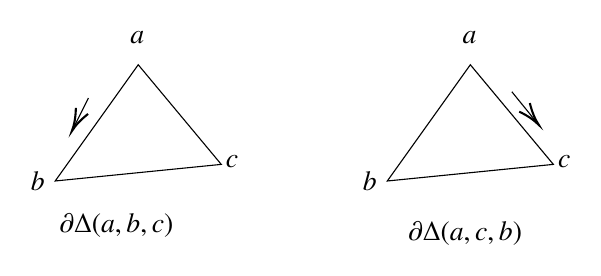
\begin{tikzpicture}[x=0.75pt,y=0.75pt,yscale=-1,xscale=1]
%uncomment if require: \path (0,476); %set diagram left start at 0, and has height of 476

%Shape: Polygon [id:ds7341302947491242] 
\draw   (216,128) -- (136,136) -- (176,80) -- cycle ;
%Straight Lines [id:da41978954017626924] 
\draw    (152,96) -- (144.89,110.21) ;
\draw [shift={(144,112)}, rotate = 296.57] [color={rgb, 255:red, 0; green, 0; blue, 0 }  ][line width=0.75]    (10.93,-3.29) .. controls (6.95,-1.4) and (3.31,-0.3) .. (0,0) .. controls (3.31,0.3) and (6.95,1.4) .. (10.93,3.29)   ;
%Shape: Polygon [id:ds08164662287981983] 
\draw   (376,128) -- (296,136) -- (336,80) -- cycle ;
%Straight Lines [id:da4173250248430085] 
\draw    (356,93) -- (367.74,107.45) ;
\draw [shift={(369,109)}, rotate = 230.91] [color={rgb, 255:red, 0; green, 0; blue, 0 }  ][line width=0.75]    (10.93,-3.29) .. controls (6.95,-1.4) and (3.31,-0.3) .. (0,0) .. controls (3.31,0.3) and (6.95,1.4) .. (10.93,3.29)   ;

% Text Node
\draw (171,62.4) node [anchor=north west][inner sep=0.75pt]    {$a$};
% Text Node
\draw (123,130.4) node [anchor=north west][inner sep=0.75pt]    {$b$};
% Text Node
\draw (217,122.4) node [anchor=north west][inner sep=0.75pt]    {$c$};
% Text Node
\draw (331,62.4) node [anchor=north west][inner sep=0.75pt]    {$a$};
% Text Node
\draw (283,130.4) node [anchor=north west][inner sep=0.75pt]    {$b$};
% Text Node
\draw (377,122.4) node [anchor=north west][inner sep=0.75pt]    {$c$};
% Text Node
\draw (137,150.4) node [anchor=north west][inner sep=0.75pt]    {$\partial \Delta ( a,b,c)$};
% Text Node
\draw (305,154.4) node [anchor=north west][inner sep=0.75pt]    {$\partial \Delta ( a,c,b)$};


\end{tikzpicture}
\end{center}
\end{example}
We now come to a theorem which plays a very important role in function theory.
\begin{theorem}
Let $\gamma$ be a closed path, let $\Omega$ be the complement of $\gamma^*$ (relative to the plane), and define 
$$
\mathrm{Ind}_{\gamma}\left( z \right) =\frac{1}{2\pi \mathrm{i}}\int_{\gamma}{\frac{\mathrm{d}\zeta}{\zeta -z}},\hspace{0.5cm}\left( z\in \Omega \right) 
$$
then $\mathrm{Ind}_\gamma$ is an integer-valued function on $\Omega$ which is constant in each component of $\Omega$ and $0$ in the unbounded component of $\Omega$.
\end{theorem}
We call $\mathrm{Ind}_\gamma(z)$ the \textbf{index} of $z$ with respect to $\gamma$. Note that $\gamma$ is compact, hence $\gamma^*$ lies in a bounded disc $D$ whose complement is connected, therefore $\Omega$ has precisely one unbounded component.
\begin{proof}
Let $[\alpha,\beta]$ be the parameter of $\gamma$, then 
$$
\mathrm{Ind}_{\gamma}\left( z \right) =\frac{1}{2\pi \mathrm{i}}\oint_{\gamma}{\frac{\mathrm{d}\zeta}{\zeta -z}}=\frac{1}{2\pi \mathrm{i}}\int_{\alpha}^{\beta}{\frac{\gamma ^{\prime}\left( s \right)}{\gamma \left( s \right) -z}\mathrm{d}s}.
$$
Note that $w/2\pi\mathrm{i}$ is an integer if and only if $e^w=1$, it suffices to show that $\varphi(\beta)=1$, where 
$$
\varphi \left( t \right) =\exp \left( \int_{\alpha}^t{\frac{\gamma ^{\prime}\left( s \right)}{\gamma \left( s \right) -z}\mathrm{d}s} \right) .
$$
Take the derivative over both sides (except possibly on a finite set $S$ that the derivative may not exist), we obtain 
$$
\varphi ^{\prime}\left( t \right) =\frac{\gamma ^{\prime}\left( t \right)}{\gamma \left( t \right) -z}\cdot \exp \left( \int_{\alpha}^t{\frac{\gamma ^{\prime}\left( s \right)}{\gamma \left( s \right) -z}\mathrm{d}s} \right) =\frac{\gamma ^{\prime}\left( t \right) \cdot \varphi \left( t \right)}{\gamma \left( t \right) -z}.
$$
Now that 
$$
\begin{aligned}
\varphi ^{\prime\prime}\left( t \right) &=\left[ \frac{\gamma ^{\prime}\left( t \right)}{\gamma \left( t \right) -z}\cdot \exp \left( \int_{\alpha}^t{\frac{\gamma ^{\prime}\left( s \right)}{\gamma \left( s \right) -z}\mathrm{d}s} \right) \right] ^{\prime}
\\
&=\frac{\gamma ^{\prime\prime}\left( t \right) \left( \gamma \left( t \right) -z \right) -\left[ \gamma ^{\prime}\left( t \right) \right] ^2}{\left( \gamma \left( t \right) -z \right) ^2}\cdot \exp \left( \int_{\alpha}^t{\frac{\gamma ^{\prime}\left( s \right)}{\gamma \left( s \right) -z}\mathrm{d}s} \right) +\left( \frac{\gamma ^{\prime}\left( t \right)}{\gamma \left( t \right) -z} \right) ^2\cdot \exp \left( \int_{\alpha}^t{\frac{\gamma ^{\prime}\left( s \right)}{\gamma \left( s \right) -z}\mathrm{d}s} \right) 
\\
&=\left( \frac{\gamma ^{\prime\prime}\left( t \right)}{\gamma \left( t \right) -z} \right) \exp \left( \int_{\alpha}^t{\frac{\gamma ^{\prime}\left( s \right)}{\gamma \left( s \right) -z}\mathrm{d}s} \right) ,
\end{aligned}
$$
therefore 
$$
\begin{aligned}
\left( \frac{\varphi \left( t \right)}{\gamma \left( t \right) -z} \right) ^{\prime}&=\left( \frac{\varphi ^{\prime}\left( t \right)}{\gamma ^{\prime}\left( t \right)} \right) ^{\prime}=\frac{\varphi ^{\prime\prime}\left( t \right) \gamma ^{\prime}\left( t \right) -\varphi ^{\prime}\left( t \right) \gamma ^{\prime\prime}\left( t \right)}{\left[ \gamma ^{\prime}\left( t \right) \right] ^2}
\\
&=\frac{1}{\left[ \gamma ^{\prime}\left( t \right) \right] ^2}\left[ \left( \frac{\gamma ^{\prime}\left( t \right) \cdot \gamma ^{\prime\prime}\left( t \right)}{\gamma \left( t \right) -z} \right) \exp \left( \int_{\alpha}^t{\frac{\gamma ^{\prime}\left( s \right)}{\gamma \left( s \right) -z}\mathrm{d}s} \right) -\frac{\gamma ^{\prime}\left( t \right) \cdot \gamma ^{\prime\prime}\left( t \right)}{\gamma \left( t \right) -z}\cdot \varphi \left( t \right) \right] =0,
\end{aligned}
$$
hence $\varphi/(\gamma-z)$ is a constant on $[\alpha,\beta]$. Since $\varphi(\alpha)=1$, we obtain 
$$
\varphi \left( t \right) =\frac{\gamma \left( t \right) -z}{\gamma \left( \alpha \right) -z},\hspace{0.5cm}\left( \alpha \le t\le \beta \right) 
$$
and since $\gamma$ is a closed path, we have $\gamma(\alpha)=\gamma(\beta)$ and hence $\varphi(\alpha)=\varphi(\beta)=1$, therefore $\mathrm{Ind}_\gamma(z)$ is an integer.\par
By Theorem 10.1.4, we have $\mathrm{Ind}_\gamma\in H(\Omega)$. Since the image of a connected set under continuous mapping is connected, we obtain $\mathrm{Ind}_\gamma$ a constant on each component of $\Omega$.\par
Finally, suppose $|z|$ is sufficiently large. Then 
$$
\left| \mathrm{Ind}_{\gamma}\left( z \right) \right|\le \int_{\gamma}{\left| \frac{1}{\zeta -z} \right|\mathrm{d}\zeta}<1,
$$
whence $\mathrm{Ind}_\gamma(z)=0$ when $z$ lies in the unbounded component of the complement of $\gamma^*$.
\end{proof}
\begin{note}\em
Now we illustrate the geometric understanding of the theorem. Suppose 
$$\lambda(t)=\int_{\alpha}^{t}\frac{\gamma^\prime(s)}{\gamma(s)-z}\mathrm{d}s.$$
Then the preceding proof shows that $2\pi\mathrm{Ind}_\gamma(z)$ is precisely the net increasing of the imaginary part of $\lambda(t)$, i.e. the net increase of the argument of $\gamma(t)-z$. If we divide this increase by $2\pi$, we obtain "the number of times that $\gamma$ winds around $z$", and this explains why the term \textbf{winding number} is used for the index.
\end{note}
 One virtue of the preceding proof is that it establishes the main properties of the index without any reference to the argument of a complex number.
 \begin{theorem}
 If $\gamma$ is the positively oriented circle with center at $a$ and radius $r$, then $\mathrm{Ind}_\gamma(z)=1$ if $|z-a|<r$, and $\mathrm{Ind}_\gamma(z)=0$ if $|z-a|>r$.
 \end{theorem}
 \begin{proof}
We take $\gamma(t)=a+re^{\mathrm{i}t}$ with $\le t\le 2\pi$. Then by Theorem  10.2.2, it suffices to show the case when $|z-a|<r$, which is 
$$
\frac{1}{2\pi \mathrm{i}}\oint_{\gamma}{\frac{\mathrm{d}\zeta}{\zeta -a}}=\frac{r}{2\pi}\int_0^{2\pi}{\left( re^{\mathrm{i}t} \right) ^{-1}\cdot e^{\mathrm{i}t}\mathrm{d}t}=1.
$$
Therefore the proof is finished.
\end{proof}
\subsection{The Local Cauchy Theorem}
There are several forms of Cauchy's theorem. They all assert that if $\gamma$ is a closed path or cycle in $\Omega$, and if $\gamma$ and $\Omega$ satisfy certain topological conditions, then the integral of every $f\in H(\Omega)$ over $\gamma$ is $0$. We shall first derive a simple local version of this which is quite sufficient for many applications. A more general global form will be established later.
\begin{theorem}
Suppose $f\in H(\Omega)$ and $F^\prime$ is continuous in $\Omega$. Then 
$$\int_\gamma F^\prime(z)\mathrm{d}z=0$$
for every closed path $\gamma\in\Omega$.
\end{theorem}
\begin{proof}
If $[\alpha,\beta]$ is the parameter interval of $\gamma$, the fundamental theorem of calculus shows that 
$$
\oint_{\gamma}{F^{\prime}\left( z \right) \mathrm{d}z}=\int_{\alpha}^{\beta}{F^{\prime}\left( \gamma \left( t \right) \right) \gamma ^{\prime}\left( t \right) \mathrm{d}t}=F\left( \gamma \left( \beta \right) \right) -F\left( \gamma \left( \alpha \right) \right) =0.
$$
This finished the proof.
\end{proof}
A simple corollary of Theorem 10.2.3 is that $\int_\gamma z^n\mathrm{d}z=0$ for all $n\in\mathbb{N}\setminus\{-1\}$ if $\gamma$ is a closed path, and $0\notin\gamma^*$ if $n<-1$. This is due to $z^n$ is the derivative of $z^{n+1}/(n+1)$ when $n\ne -1$. The condition that $n=-1$ has been dealt with in the previous section.\par
Now we introduce the following \textbf{Cauchy's Theorem in a triangle}.
\begin{theorem}
Suppose $\Delta$ is a closed triangle in a plane open set $\Omega$, $p\in\Omega$, and $f$ is continuous on $\Omega$ such that $f\in H(\Omega\setminus\{p\})$. Then 
$$\int_{\partial\Delta}f(z)\mathrm{d}z=0.$$
\end{theorem}
\begin{proof}
We assume that $p\notin\Delta$ first. Suppose the three vertices of $\Delta$ are $a,b$ and $c$. Let $a^\prime$, $b^\prime$ and $c^\prime$ be the midpoint of the opposite side relative to $a$, $b$ and $c$, then define four triangles 
$$
\Delta ^1=\Delta \left\{ a,c^{\prime},b^{\prime} \right\} ,\Delta ^2=\Delta \left\{ b,a^{\prime},c^{\prime} \right\} ,\Delta ^3=\Delta \left\{ c,b^{\prime},a^{\prime} \right\} ,\Delta ^4=\Delta \left\{ a^{\prime},b^{\prime},c^{\prime} \right\}. 
$$
Now if $J$ is the value of $\oint_{\partial\Delta}f(z)\mathrm{d}z$, then 
$$
J=\sum_j{\int_{\partial \Delta ^j}{f\left( z \right) \mathrm{d}z}}.
$$
Clearly there exists some triangle, say $\Delta_1\in\{\Delta^j\}_j$, such that 
$$
\left| \int_{\partial \Delta ^i}{f\left( z \right) \mathrm{d}z} \right|>\left| \frac{J}{4} \right|.
$$
Repeat the previous operation on $\Delta_1$, we obtain a sequence of triangles $\Delta \supset \Delta _1\supset \cdots \supset \Delta _n\supset \cdots $ such that the length of $\partial\Delta_n$ is $2^{-n}L$, where $L$ is the length of $\partial\Delta$. Therefore 
$$
\left| J \right|\le 4\left| \int_{\partial \Delta _1}{f\left( z \right) \mathrm{d}z} \right|\le 4^2\left| \int_{\partial \Delta _2}{f\left( z \right) \mathrm{d}z} \right|\le \cdots \le 4^n\left| \int_{\partial \Delta _n}{f\left( z \right) \mathrm{d}z} \right|.
$$
Since each $\Delta_k$ is compact, there exists a unique $z_0\in\bigcap_{n}\Delta_n$. Since $p\notin\Delta$, $f$ is differentiable at $z_0$. Let $\varepsilon>0$. Then there corresponds $r>0$ such that 
$$
\left| f\left( z \right) -f\left( z_0 \right) -f^{\prime}\left( z \right) \left( z-z_0 \right) \right|\le \varepsilon \left| z-z_0 \right|,\hspace{0.5cm}\left( \left| z-z_0 \right|<r \right) 
$$
whence 
$$
\left| \int_{\partial \Delta _n}{f\left( z \right) \mathrm{d}z} \right|=\left| \int_{\partial \Delta _n}{\left[ f\left( z \right) -f\left( z_0 \right) -f^{\prime}\left( z \right) \left( z-z_0 \right) \right] \mathrm{d}z} \right|\le \varepsilon \cdot 2^{-n}L\cdot r.
$$
Since there exists some large $n$ such that $r<2^{-n}L$, we obtain 
$$
\left| \int_{\partial \Delta _n}{f\left( z \right) \mathrm{d}z} \right|\le \varepsilon \cdot \left( 2^{-n}L \right) ^2=\frac{\varepsilon L^2}{4^n}.
$$
Therefore 
$$
J=\left| \int_{\partial \Delta _n}{f\left( z \right) \mathrm{d}z} \right|\le \frac{\varepsilon L^2}{4^n}\rightarrow 0,
$$
hence $J=0$ and the proof is finished.\par
Now suppose $p$ is a vertex of $\Delta$, say $p=a$. Then we may divide the triangle $\Delta$ into three small triangles, $\Delta \left( a,x,y \right) ,\Delta \left( x,b,y \right) ,\Delta \left( b,c,y \right) $, as shown below:
\begin{center}


\tikzset{every picture/.style={line width=0.75pt}} %set default line width to 0.75pt        

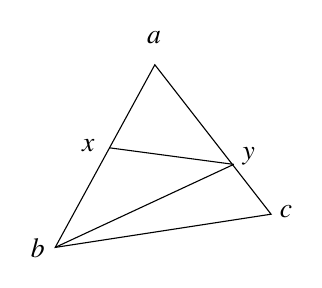
\begin{tikzpicture}[x=0.75pt,y=0.75pt,yscale=-1,xscale=1]
%uncomment if require: \path (0,476); %set diagram left start at 0, and has height of 476

%Shape: Polygon [id:ds944599867727798] 
\draw   (216,136) -- (168,224) -- (272,208) -- cycle ;
%Straight Lines [id:da763895858654525] 
\draw    (194,176) -- (254,184) ;
%Straight Lines [id:da18568190298138365] 
\draw    (168,224) -- (254,184) ;

% Text Node
\draw (211,118.4) node [anchor=north west][inner sep=0.75pt]    {$a$};
% Text Node
\draw (155,218.4) node [anchor=north west][inner sep=0.75pt]    {$b$};
% Text Node
\draw (275,202.4) node [anchor=north west][inner sep=0.75pt]    {$c$};
% Text Node
\draw (179,170.4) node [anchor=north west][inner sep=0.75pt]    {$x$};
% Text Node
\draw (257,174.4) node [anchor=north west][inner sep=0.75pt]    {$y$};


\end{tikzpicture}
\end{center}
therefore 
$$
\int\limits_{\partial \Delta}{f\left( z \right) \mathrm{d}z}=\int\limits_{\partial \Delta \left( a,x,y \right)}{f\left( z \right) \mathrm{d}z}+\int\limits_{\partial \Delta \left( x,b,y \right)}{f\left( z \right) \mathrm{d}z}+\int\limits_{\partial \Delta \left( b,c,y \right)}{f\left( z \right) \mathrm{d}z}=\int\limits_{\partial \Delta \left( a,x,y \right)}{f\left( z \right) \mathrm{d}z}.
$$
Then since $f$ is continuous on $\Delta$, we may let $x$ and $y$ arbitrarily close to $a$, therefore the integral $\int_{\partial\Delta(a,x,y)}f(z)\mathrm{d}z$ converges to zero, and hence $\int_{\partial\Delta}f(z)\mathrm{d}z=0$ holds for this condition.\par
Now suppose $p$ lies in the interior of $\Delta$, such condition may be easily deduced into the condition of two previous conditions, therefore our proof is finished.
\end{proof}
Our next theorem is the \textbf{Cauchy's theorem in a convex open set}.
\begin{theorem}
Let $\Omega$ be a convex open set, $p\in\Omega$, $f$ is continuous on $\Omega$ and $f\in H(\Omega\setminus\{p\})$. Then 
$$\int_\gamma f(z)\mathrm{d}z=0$$
for all closed path $\gamma\in\Omega$.
\end{theorem}
\begin{proof}
Let $a\in\Omega$. Since $\Omega$ is convex, the line $[a,z]$ lies in $\Omega$ for all $z\in\Omega$. Therefore we may define the integral 
$$
F\left( z \right) =\int_{\left[ a,z \right]}{f\left( \zeta \right) \mathrm{d}\zeta}.\hspace{0.5cm}\left( z\in \Omega \right) 
$$
Now consider $z_0\in\Omega$. Since $a,z$ and $z_0$ forms a triangle, we apply Theorem 10.3.2 to obtain 
$$
\int_{\partial \Delta}{f\left( \zeta \right) \mathrm{d}\zeta}=\int_{\left[ a,z \right]}{f\left( \zeta \right) \mathrm{d}\zeta}+\int_{\left[ z,z_0 \right]}{f\left( \zeta \right) \mathrm{d}\zeta}+\int_{\left[ z_0,a \right]}{f\left( \zeta \right) \mathrm{d}\zeta}=0,
$$
hence 
$$
\int_{\left[ z_0.z \right]}{f\left( \zeta \right) \mathrm{d}\zeta}=\int_{\left[ a,z \right]}{f\left( \zeta \right) \mathrm{d}\zeta}-\int_{\left[ a,z_0 \right]}{f\left( \zeta \right) \mathrm{d}\zeta}.
$$
Therefore 
$$
\frac{F\left( z \right) -F\left( z_0 \right)}{z-z_0}-f\left( z_0 \right) =\frac{1}{z-z_0}\int_{\left[ z_0,z \right]}{f\left( \zeta \right) \mathrm{d}\zeta}-f\left( z_0 \right) =\frac{1}{z-z_0}\int_{\left[ z_0,z \right]}{\left[ f\left( \zeta \right) -f\left( z_0 \right) \right] \mathrm{d}\zeta}.
$$
Since $f$ is continuous in $\Omega$, for all $\varepsilon>0$ there exists some $\delta>0$, such that when $|\zeta-z_0|<\delta$ we have $|f(\zeta)-f(z_0)|<\varepsilon$. Now let $z_0\to z$, we have 
$$
\left| \frac{F\left( z \right) -F\left( z_0 \right)}{z-z_0}-f\left( z_0 \right) \right|\le \frac{1}{\left| z-z_0 \right|}\cdot \varepsilon \cdot \left| z-z_0 \right|=\varepsilon ,
$$
therefore $F^\prime(z_0)=f(z_0)$. Since $z_0$ is arbitrarily chosen, we may conclude that 
$$
\int_{\gamma}{f\left( z \right) \mathrm{d}z}=\int_{\gamma}{F^{\prime}\left( z \right) \mathrm{d}z}=0,
$$
where the last equality follows from theorem 10.3.1.
\end{proof}
\begin{theorem}
Let $\Omega$ be an open convex set, $f\in H(\Omega)$. Suppose $\gamma$ is a closed path, $z\in\Omega$ and $z\notin\gamma^*$, then 
$$
f\left( z \right) \cdot \mathrm{Ind}_{\gamma}\left( z \right) =\frac{1}{2\pi \mathrm{i}}\int_{\gamma}{\frac{f\left( \zeta \right)}{\zeta -z}\mathrm{d}\zeta}.
$$
\end{theorem}
\begin{proof}
We consider the function 
$$
g\left( \zeta \right) =\begin{cases}
	\frac{f\left( \zeta \right) -f\left( z \right)}{\zeta -z},\zeta \in \Omega \setminus \left\{ z \right\} ,\\
	f^{\prime}\left( z \right) ,\zeta =z.\\
\end{cases}
$$
Then clearly $g^\prime(\zeta)$ is holomorphic, therefore apply Theorem 10.3.3, we obtain 
$$
0=\frac{1}{2\pi \mathrm{i}}\int_{\gamma}{g\left( \zeta \right) \mathrm{d}\zeta}=\frac{1}{2\pi \mathrm{i}}\int_{\gamma}{\frac{f\left( \zeta \right) -f\left( z \right)}{\zeta -z}\mathrm{d}\zeta}=\frac{1}{2\pi \mathrm{i}}\int_{\gamma}{\frac{f\left( \zeta \right)}{\zeta -z}\mathrm{d}\zeta}-f\left( z \right) \cdot \frac{1}{2\pi \mathrm{i}}\int_{\gamma}{\frac{\mathrm{d}\zeta}{\zeta -z}},
$$
hence 
$$
f\left( z \right) \cdot \mathrm{Ind}_{\gamma}\left( z \right) =f\left( z \right) \cdot \frac{1}{2\pi \mathrm{i}}\int_{\gamma}{\frac{\mathrm{d}\zeta}{\zeta -z}}=\frac{1}{2\pi \mathrm{i}}\int_{\gamma}{\frac{f\left( \zeta \right)}{\zeta -z}\mathrm{d}\zeta}.
$$
This finished the proof.
\end{proof}
We now come to an easy corollary of Theorem 10.3.4, which answered the question about the converse of Theorem 10.1.2.
\begin{theorem}
Suppose $\Omega$ is an open set. Let $f$ be a holomorphic function on $\Omega$, then $f$ is representable by power series in $\Omega$.
\end{theorem}
\begin{proof}
Since $\omega$ is open, for all $a\in\Omega$ there exists an open disc $D(a,R)$ such that $D(a,R)\subset\Omega$. Now take $\gamma$ an oriented circle centered at $a$ with radius $r<R$, then 
$$
f\left( z \right) =f\left( z \right) \cdot \mathrm{Ind}_{\gamma}\left( z \right) =\frac{1}{2\pi \mathrm{i}}\int_{\gamma}{\frac{f\left( \zeta \right)}{\zeta -z}\mathrm{d}\zeta}.\hspace{0.5cm}\left( z\in D\left( a,r \right) \right) 
$$
However by Theorem 10.1.4 with $X=2\pi$, $\mathrm{d}\mu(\zeta)=f(\gamma(z))\gamma^\prime(z)\mathrm{d}z$ and $\varphi(z)=\gamma(z)$, we conclude that $f(z)$ is representable by a power series in $D(a,R)$. Since the representation is valid for every $z\in D(a,R)$, the proof is complete.
\end{proof}
The Cauchy theorem has a useful reverse, which is usually called the \textbf{Morera's theorem}: 
\begin{theorem}
Suppose $f$ is a complex function in an open set $\Omega$ such that 
$$\int_{\partial\Delta}f(z)\mathrm{d}z=0$$
for all triangle $\Delta\subset\Omega$, then $f\in H(\Omega)$.
\end{theorem}
\begin{proof}
Let $V$ be a convex subset of $\Omega$, then by the proof of Theorem 10.3.3 we may construct a function $F$ such that $F\in H(\Omega)$ and $F^\prime=f$. Therefore $f$ is the derivative of a holomorphic function, which is also holomorphic.
\end{proof}
\subsection{The Power Series Representation}
The fact that every holomorphic function is locally the sum of a convergent power series has a large number of interesting consequences. A few of these are developed in this section.
\begin{theorem}
Suppose $\Omega$ is a region, $f\in H(\Omega)$, and $Z(f)=\{a\in\Omega:f(a)=0\}$. Then either $Z(f)=\Omega$, or $Z(f)$ has no limit point in $\Omega$. In the latter case there corresponds to each $a\in Z(f)$ a unique positive integer $m=m(a)$ such that 
$$f(z)=(z-a)^mg(z),\hspace{0.5cm}(z\in\Omega)$$
where $g\in H(\Omega)$ and $g(a)\ne 0$. Furthermore, $Z(f)$ is at most countable.
\end{theorem}
\begin{proof}
Let $A$ be the set of all limit points of $Z(f)$. Now suppose $a\in Z(f)$, choose $r>0$ such that 
$$
f\left( z \right) =\sum_{n=0}^{\infty}{c_n\left( z-a \right) ^n},\hspace{0.5cm}z\in D\left( a,r \right) .
$$
Now there are two possibilities: $c_n=0$ for all $n\in\mathbb{N}$, or there exists a minimum $m\in\mathbb{N}$ such that $c_m\ne 0$. Now if it is the latter case, we define 
$$
g\left( z \right) =\begin{cases}
	\frac{f\left( z \right)}{\left( z-a \right) ^m},z\in \Omega \setminus \left\{ a \right\} ,\\
	c_m,z=a.\\
\end{cases}
$$
whence 
$$
f\left( z \right) =\left( z-a \right) ^mg\left( z \right) ,\hspace{0.5cm}g\in H\left( \Omega \setminus \left\{ a \right\} \right) .
$$
But observe that 
$$
f\left( z \right) =\left( z-a \right) ^mg\left( z \right) =\sum_{n=0}^{\infty}{c_n\left( z-a \right) ^n}=\sum_{k=0}^{\infty}{c_{m+k}\left( z-a \right) ^{m+k}},
$$
we have 
$$
g\left( z \right) =\sum_{k=0}^{\infty}{c_{n+k}\left( z-a \right) ^k},\hspace{0.5cm}z\in D\left( a,r \right) .
$$
Therefore $g\in H(\Omega)$. Since $g$ is continuous on $\Omega$, in particular continuous at $a$, we have $a$ an isolated point in $Z(f)$.\par
Now suppose $a\in A$. Then the first case, i.e. $c_n=0$ for all $n\in\mathbb{N}$, must occur. Therefore $f$ is a constant and hence $a$ is an interior of $A$, therefore $A$ is open. Now consider $B=\Omega\setminus A$, which, by definition of $A$, is also open. Therefore $\Omega$ is the disjoint union of two open sets, and by the connectivity of $\Omega$ we have either $A=\Omega$ and $B=\Omega$. If $A=\Omega$, then $Z(f)=\Omega$. If $B=\Omega$, then $A=\emptyset$, hence $Z(f)$ has at most finite many points in a compact subset of $\Omega$. Since $\Omega$ is $\sigma$-compact, we have $Z(f)$ contains at most countably many points.
\end{proof}
\begin{note}\em
(a) The integer $m$ in Theorem 10.4.1 is called the \textbf{order} of the zero which $f$ has at the point $a$. Clearly $Z(f)=\Omega$ if and only if $f$ is identically $0$ in $\Omega$. We call $Z(f)$ the \textbf{zero set} of $f$. Analogous results hold of course for the set of $\alpha$-points of $f$, i.e. the zero set of $f-\alpha$, where $\alpha$ is any complex number.\par
(b) The theorem may fail if the condition $\Omega$ is connected is omitted. For example, consider $\Omega=\Omega_1\cup\Omega_2$, where $\Omega_1$ and $\Omega_2$ are disjoint connected open sets. Put $f(z)=1$ for $z\in\Omega_1$ and $f(z)=0$ for $z\in\Omega_2$.
\end{note}
\begin{corollary}
If $f$ and $g$ are holomorphic functions in a region $\Omega$ and if $f(z)=g(z)$ for all $z$ in some set which has a limit point $\Omega$, then $f(z)=g(z)$ for all $z\in\Omega$.
\end{corollary}
\begin{proof}
Let $h(z)=f(z)-g(z)$ and $Z(h)$ defined similar to the way in Theorem 10.4.1. Then $Z(h)$ contains a limit point in $\Omega$, hence $Z(h)=\Omega$ by Theorem 10.4.1. Therefore $f(z)-g(z)=0$ for all $z\in\Omega$, which is $f(z)=g(z)$ for all $z\in\Omega$.
\end{proof}
\begin{definition}
If $a\in\Omega$ and $f\in H(\Omega\setminus\{a\}$, then $f$ is said to have an \textbf{isolated singularity} at the point $a$. If $f$ can be so defined at $a$ that the extended function is holomorphic in $\Omega$, the singularity is said to be \textbf{removable}.
\end{definition}
We have the following theorem for removable singularities:
\begin{theorem}
Suppose $f\in H(\Omega\setminus\{a\})$ and $f$ is bounded in $D^\prime(a,r)$ for some $r>0$. Then $f$ has a removable singularity at $a$.
\end{theorem}
\begin{proof}
We define the function 
$$
h\left( z \right) =\begin{cases}
	\left( z-a \right) ^2f\left( z \right) ,z\in \Omega \setminus \left\{ a \right\} ,\\
	0,z=a,\\
\end{cases}
$$
then by the assumption that $f$ is bounded, we have 
$$
h^{\prime}\left( a \right) =\lim_{z\rightarrow a} \frac{h\left( z \right) -h\left( a \right)}{z-a}=\lim_{z\rightarrow a} \frac{\left( z-a \right) ^2f\left( z \right)}{z-a}=\lim_{z\rightarrow a} \left( z-a \right) f\left( z \right) =0.
$$
Clearly $h$ is differentiable at every point of $\Omega\setminus\{a\}$, then $h$ is holomorphic on $\Omega$. Therefore suppose 
$$
h\left( z \right) =\sum_{n=2}^{\infty}{c_n\left( z-a \right) ^n},\hspace{0.5cm}z\in D\left( a,r \right) ,
$$
we have 
$$
f\left( z \right) =\frac{h\left( z \right)}{\left( z-a \right) ^2}=\sum_{n=0}^{\infty}{c_{n+2}\left( z-a \right) ^n}
$$
by defining $f(a)=c_2$. Therefore $f$ is representable by power series in $D(a,r)$, hence holomorphic.
\end{proof}
\begin{theorem}
If $a\in\Omega$ and $f\in H(\Omega\setminus\{a\})$, then one of the following conditions must be true:\par
(a) $f$ has a removable singularity.\par
(b) There exists $m\in\mathbb{N}$ that $m\ge 1$ and $c_1,\cdots,c_m\in\mathbb{C}$ such that 
$$
f\left( z \right) -\sum{\frac{c_k}{\left( z-a \right) ^k}}
$$
has a removable singularity.\par
(c) If $r>0$ and $D(a,r)\subset\Omega$, then $f(D^\prime(a,r))$ is dense in $\mathbb{C}$.
\end{theorem}
\begin{proof}
Suppose that (c) is false. Then there exists some $r>0$ and $\delta>0$, and for some $w\in\mathbb{C}$ such that $|f(z)-w|>\delta$ for all $z\in D^\prime(a,r)$. Let us now write $D$ for $D(a,r)$ and $D^\prime$ for $D^\prime$. Define 
$$
g\left( z \right) =\frac{1}{f\left( z \right) -w},\hspace{0.5cm}z\in D^{\prime}\left( a,r \right) .
$$
Clearly $|g|\le 1/\delta$, therefore by Theorem 10.4.4 we obtain $a$ is a removable singularity of $g$, and we may suppose $g\in H(D)$.\par
If $g(a)\ne 0$, then $f(a)$ is finite. Therefore $f$ is finite on $D$ and hence by Theorem 10.4.4 we obtain $a$ is a removable singularity of $f$, which is condition (a).\par
If $g(a)=0$, then suppose $a$ is a zero of order $m\ge 1$. By Theorem 10.4.1, there exists some $g_1(z)\in H(D)$ with $g_1(a)\ne 0$ such that 
$$
g\left( z \right) =\left( z-a \right) ^mg_1\left( z \right) ,\hspace{0.5cm}z\in D\left( a,r \right) .
$$
Now that $g_1(a)\ne 0$, we may define $h(z)=1/g_1(z)$ for $z\in D$, which is clearly a holomorphic function. Now that 
$$
f\left( z \right) -w=\frac{1}{g\left( z \right)}=\frac{1}{\left( z-a \right) ^mg_1\left( z \right)}=\frac{h\left( z \right)}{\left( z-a \right) ^m}.
$$
However $h\in H(D)$, therefore $h$ may be represented by power series in $D$ as follows: 
$$
h\left( z \right) =\sum_{n=0}^{\infty}{b_n\left( z-a \right) ^n},\hspace{0.5cm}z\in D^{\prime}\left( a,r \right) .
$$
Therefore 
$$
f\left( z \right) -w=\frac{1}{\left( z-a \right) ^m}\sum_{n=0}^{\infty}{b_n\left( z-a \right) ^n},
$$
and hence 
\begin{small}
$$
f\left( z \right) -\sum_{k=1}^m{\frac{b_{m-k}}{\left( z-a \right) ^k}}=w+\sum_{n=0}^{\infty}{b_n\left( z-a \right) ^{n-m}}-\sum_{k=1}^m{b_{m-k}\left( z-a \right) ^{-k}}=w+\sum_{n=m}^{\infty}{b_n\left( z-a \right) ^n}\in H\left( D^{\prime} \right) .
$$
\end{small}
Therefore the condition (b) is true.
\end{proof}
\begin{note}\em
In case (b), $f$ is said to have a \textbf{pole of order $m$} at $a$. The function $\sum c_k(z-a)^{-k}$ is called the \textbf{principal part} of $f$ at $a$.\par
In case (c), $f$ is said to have a \textbf{essential singularity} at $a$. A statement equivalent to (c) is that to each $w\in\mathbb{C}$ there corresponds a sequence $\{z_n\}$ such that $z_n\to a$ and $f(z_n)\to w$ as $n\to\infty$.
\end{note}
We now exploit the fact that the restriction of a power series $\sum c_n(z-a)^n$ to a circle with center at $a$ is a trigonometric series.
\begin{theorem}
If 
$$
f\left( z \right) =\sum_{n=0}^{\infty}{c_n\left( z-a \right) ^n},\hspace{0.5cm}z\in D\left( a,R \right) ,
$$
and if $0<r<R$, then 
$$
\sum_{n=0}^{\infty}{\left| c_n \right|^2r^{2n}}=\frac{1}{2\pi}\int_{-\pi}^{\pi}{\left| f\left( a+re^{\mathrm{i}\theta} \right) \right|^2\mathrm{d}\theta}.
$$
\end{theorem}
\begin{proof}
We have 
$$
f\left( a+re^{\mathrm{i}\theta} \right) =\sum_{n=0}^{\infty}{c_nr^ne^{\mathrm{i}n\theta}}.
$$
For $r<R$, the series converges uniformly on $[-\pi,\pi]$. Therefore by the Inversion formula we have 
$$
c_nr^n=\frac{1}{2\pi}\int_{-\pi}^{\pi}{f\left( a+re^{\mathrm{i}\theta} \right) e^{-\mathrm{i}n\theta}\mathrm{d}\theta},
$$
and hence 
$$
\sum_{n=0}^{\infty}{\left| c_n \right|^2r^{2n}}=\frac{1}{2\pi}\int_{-\pi}^{\pi}{\left| f\left( a+re^{\mathrm{i}\theta} \right) \right|^2\mathrm{d}\theta}
$$
by Parseval identity.
\end{proof}
Here are some consequences:
\begin{theorem}{\textbf{(Liouville)}}
Every bounded entire function is constant.
\end{theorem}
\begin{proof}
Let $f$ be an entire function and $|f(z)|<M$ for all $z\in\mathbb{C}$. Suppose $f(z)=\sum c_nz^n$ for some $c_n\in\mathbb{C}$, then by Theorem 10.4.6 we have 
$$
\sum_{n=0}^{\infty}{\left| c_n \right|^2r^{2n}}\le M^2
$$
for all $r\in\mathbb{C}$, therefore $c_n=0$ for all $n\ge 1$, and hence $f$ is a constant.
\end{proof}
\begin{theorem}{\textbf{(The Maximum Modulus Theorem)}}
Suppose $\Omega$ is a region, $f\in H(\Omega)$, and $\overline{D}(a,r)\subset\Omega$. Then 
$$
\left| f\left( a \right) \right|\le \max_{\theta} \left| f\left( a+e^{\mathrm{i}\theta} \right) \right|,
$$
and the equality holds if and only if $f$ is a constant.
\end{theorem}
\begin{proof}
Suppose $\left| f\left( a+e^{\mathrm{i}\theta} \right) \right|\le \left| f\left( a \right) \right|$ for all $\theta$. Then 
$$
\sum_{n=0}^{\infty}{\left| c_n \right|^2r^{2n}}\le \left| f\left( a \right) \right|^2=c_{0}^{2},
$$
which implies $c_n=0$ for all $n\ge 1$ and hence $f$ a constant.
\end{proof}
\begin{corollary}
Under the same hypothesis of Theorem 10.4.8, we have 
$$
\left| f\left( a \right) \right|\ge \min_{\theta} \left| f\left( a+e^{\mathrm{i}\theta} \right) \right|
$$
if $f$ has no zero in $D(a,r)$.
\end{corollary}
\begin{proof}
The condition is trivial if $f(a+e^{\mathrm{i}\theta})=0$ for some $\theta$. Otherwise consider $1/f$, which is holomorphic since $f$ has no zeros in $D(a,r)$. Apply the maximum modulus theorem on $1/f$, we have 
$$
\left| \frac{1}{f\left( a \right)} \right|\le \max_{\theta} \left| \frac{1}{f\left( a+e^{\mathrm{i}\theta} \right)} \right|,
$$
which is 
$$
\left| f\left( a \right) \right|\ge \min_{\theta} \left| f\left( a+e^{\mathrm{i}\theta} \right) \right|.
$$
This completes the proof.
\end{proof}
\begin{theorem}{\textbf{(Fundamental Theorem of Algebra)}}
If $n$ is a positive number and 
$$
P\left( z \right) =z^n+a_{n-1}z^{n-1}+\cdots +a_1z+a_0,
$$
where $a_i\in\mathbb{C}$ for all $i=0,1,2,\cdots,n-1$, then $P$ has precisely $n$ zeros (up to multiplicities) in the plane.
\end{theorem}
\begin{proof}
We first obverse that 
$$
\left| P\left( z \right) \right|\ge \left| z \right|^n-\left| a_{n-1} \right|\cdot \left| z \right|^{n-1}-\cdots -\left| a_1 \right|\cdot \left| z \right|-\left| a_0 \right|=\left| z \right|^n\cdot \left( 1-\left| \frac{a_{n-1}}{z} \right|-\cdots -\left| \frac{a_0}{z^n} \right| \right) \rightarrow \infty 
$$
as $|z|\to\infty$, therefore we may pick some large $r$ such that $|P(re^{\mathrm{i}\theta})>|P(0)|$. Now suppose there are no zeros of $P$ on $\mathbb{C}$, then $1/P$ is entire. Hence apply the maximum modulus theorem to $1/P$, we have 
$$
\left| f\left( 0 \right) \right|\le \max_{\theta} \left| f\left( re^{\mathrm{i}\theta} \right) \right|,
$$
which is a contradiction. Therefore $P$ has at least one zero. Suppose now $P(z_1)=0$, then there exists some $P_1$ such that $P_1(z_1)\ne 0$, and $P(z)=(z-z_1)P_1(z)$. Now the theorem is proved via induction.
\end{proof}
\begin{note}\em
This theorem contains the fact that $\mathbb{C}$ is \textbf{algebraically closed}, i.e. every nonconstant polynomial with complex coefficients has at least one complex zero.
\end{note}
\begin{theorem}{\textbf{(Cauchy's Estimates)}}
If $f\in H(D(a,R))$ and $|f(z)|\le M$ for all $z\in D(a,R)$, then 
$$|f^{(n)}(a)|\le\frac{n!M}{R^n}.\hspace{0.5cm}(n=1,2,3,\cdots)$$
\end{theorem}
\begin{proof}
By Cauchy's Formula we have 
$$
f\left( z \right) =\frac{1}{2\pi \mathrm{i}}\oint_{D\left( a,R \right)}{\frac{f\left( \zeta \right)}{\zeta -z}\mathrm{d}\zeta}.
$$
Now observe that 
$$
\frac{f\left( z \right) -f\left( z_0 \right)}{z-z_0}=\frac{1}{2\pi \mathrm{i}\cdot \left( z-z_0 \right)}\int_{D\left( a,R \right)}{\left( \frac{f\left( \zeta \right)}{\zeta -z}-\frac{f\left( \zeta \right)}{\zeta -z_0} \right) \mathrm{d}\zeta}=\frac{1}{2\pi \mathrm{i}}\int_{D\left( a,R \right)}{\frac{f\left( \zeta \right)}{\left( \zeta -z \right) \left( \zeta -z_0 \right)}\mathrm{d}\zeta},
$$
we conclude that 
$$
f^{\prime}\left( z \right) =\lim_{z\rightarrow z_0} \frac{f\left( z \right) -f\left( z_0 \right)}{z-z_0}=\frac{1}{2\pi \mathrm{i}}\int_{D\left( a,R \right)}{\frac{f\left( \zeta \right)}{\left( \zeta -z \right) ^2}\mathrm{d}\zeta}.
$$
Therefore by induction we have  
$$
f^{\left( n \right)}\left( z \right) =\frac{n!}{2\pi \mathrm{i}}\int_{D\left( a,R \right)}{\frac{f\left( \zeta \right)}{\left( \zeta -z \right) ^{n+1}}\mathrm{d}\zeta}.
$$
Hence 
$$
\left| f^{\left( n \right)}\left( a \right) \right|\le \frac{n!}{2\pi}\int_{D\left( a,R \right)}{\left| \frac{f\left( \zeta \right)}{\left( \zeta -a \right) ^{n+1}} \right|\mathrm{d}\zeta}=\frac{n!}{2\pi}\int_0^{2\pi}{\left| \frac{f\left( a+re^{\mathrm{i}\theta} \right)}{r^{n+1}\cdot e^{\mathrm{i}\left( n+1 \right) \theta}} \right|\mathrm{d}\theta}\le \frac{n!M}{R^n},
$$
which finished the proof.
\end{proof}
\begin{note}\em
To see that the inequality in Theorem 10.4.11 can't be improved, take $a=0$, $R=1$ and $f(z)=z^n$.
\end{note}
\begin{definition}
A sequence $\{f_j\}$ of functions in $\Omega$ is said to be \textbf{converge to $f$ uniformly on compact subsets of $\Omega$} if to every compact subset $K\subset\Omega$ and to every $\varepsilon>0$, there corresponds an $N=N(K,\varepsilon)$ such that $|f_j(z)-f(z)|<\varepsilon$ for all $z\in K$ if $j>N$.
\end{definition}
For instance, the function $f(z)=z^n$ converges uniformly on compact subsets of $D(0,1)$, but not uniformly on $D(0,1)$.\par
It is uniform convergence on compact subsets which arises most naturally in connection with limit operations on holomorphic functions. The term \textbf{almost uniform convergence} is sometimes used for this concept.
\begin{theorem}
Suppose $f_j\in H(\Omega)$ for $j=1,2,3,\cdots$, and $f_j\to f$ uniformly on compact subsets of $\Omega$. Then $f\in H(\Omega)$, and $f^\prime_j\to f^\prime$ uniformly on compact subsets of $\Omega$.
\end{theorem}
\begin{proof}
We first show that $f\in H(\Omega)$. Since $f_j\in H(\Omega)$, for any compact triangle $\Delta\subset\Omega$, we have 
$$
\int_{\partial \Delta}{f\left( z \right) \mathrm{d}z}=\lim_{j\rightarrow \infty} \int_{\partial \Delta}{f_j\left( z \right) \mathrm{d}z}=0,
$$
therefore by Morera's theorem we have $f\in H(\Omega)$.\par
Now let $K$ be compact subset of $\Omega$. Then there exists some $R>0$ such that to each $z\in K$, the disc $\overline{D}(z,R)$ is compact in $\Omega$. Now to each $z\in K$ apply Cauchy's estimates, we have 
$$
\left| f^{\prime}\left( z \right) -f_{j}^{\prime}\left( z \right) \right|\le \frac{1}{R}\cdot \mathop {\mathrm{sup}} \limits_{z\in \overline{D}\left( z,R \right)}\left| f\left( z \right) -f_j\left( z \right) \right|\rightarrow 0,\hspace{0.5cm}\left( j\rightarrow \infty \right) 
$$
therefore $f_j^\prime\to f_j$ uniformly on $K$.
\end{proof}
An immediate consequence of Theorem 10.4.13 is that, under the same hypothesis, we have $f_j^{(n)}\to f^{(n)}$ uniformly, as $j\to\infty$, on every compact subset of $\Omega$, and for every positive integer $n$. Compare to the situation on the real line, where sequences of infinitely differentiable functions can converge uniformly to nowhere differentiable functions!
\subsection{The Open Mapping Theorem}
Consider the following problem: If $\Omega$ is a region and $f\in H(\Omega)$, what can we say about $f(\Omega)$? Indeed, $f(\Omega)$ is either a region or a point. This important property will be developed in this section, and we shall answer it with a more detailed theorem.
\begin{lemma}\em
If $f\in H(\Omega)$ and $g$ is defined on $\Omega\times\Omega$ by 
$$
g\left( z,w \right) =\begin{cases}
	\frac{f\left( z \right) -f\left( w \right)}{z-w},w\ne z,\\
	f^{\prime}\left( z \right) ,w=z,\\
\end{cases}
$$
then $g$ is continuous in $\Omega\times\Omega$.
\end{lemma}
\begin{proof}
The only points at which the continuity of $g$ is possibly in doubt is $z=w$. Now fix $a\in\Omega$, then there exists some $r>0$ such that for all $\zeta\in\Omega$, we have $|f^\prime(\zeta)-f^\prime(z)|<\varepsilon$. Now take $z,w\in D(a,r)$, we have 
$$
\left| g\left( z,w \right) -g\left( a,a \right) \right|=\left| \frac{f\left( z \right) -f\left( w \right)}{z-w}-f^{\prime}\left( a \right) \right|\le \int_0^1{\left| f^{\prime}\left( \left( 1-t \right) z+tw \right) -f^{\prime}\left( a \right) \right|\mathrm{d}z}<\varepsilon ,
$$
whence $f$ is continuous at the point $(a,a)$, which finished the proof.
\end{proof}
\begin{theorem}
Suppose $\varphi\in H(\Omega)$, $z_0\in\Omega$ and $\varphi^\prime(z_0)\ne 0$. Then $\Omega$ contains a neighborhood $V$ of $z_0$ such that \par
(i) $\varphi$ is one-to-one in $V$;\par
(ii) $W=\varphi(V)$ is an open set, and \par
(iii) If $\psi:W\to V$ is defined by $\psi(\varphi(z))=z$, then $\psi\in H(W)$.
\end{theorem}
\begin{proof}
(i) Apply Lemma 10.5.1 to $\varphi$, we obtain that there exists some neighborhood $V$ of $z_0$ such that 
$$
\left| \varphi \left( z_1 \right) -\varphi \left( z_2 \right) \right|\ge \frac{1}{2}\left| \varphi ^{\prime}\left( z_0 \right) \right|\cdot \left| z_1-z_2 \right|,\hspace{0.5cm}\left( z_1,z_2\in V \right) 
$$
whence $\varphi$ is one-to-one in $V$.\par
(ii) Pick $a\in V$, then there exists some $r>0$ such that $\overline{D}(a,r)\in V$. By (i) there exists some $c>0$ such that 
$$
\left| \varphi \left( a+re^{\mathrm{i}\theta} \right) -\varphi \left( a \right) \right|>2c,\hspace{0.5cm}\left( -\pi \le \theta \le \pi \right) 
$$
therefore for each $\lambda\in D(\varphi(a),c)$, we have 
$$
\begin{aligned}
\left| \lambda -\varphi \left( a+re^{\mathrm{i}\theta} \right) \right|&=\left| \lambda -\varphi \left( a \right) +\varphi \left( a \right) -\varphi \left( a+re^{\mathrm{i}\theta} \right) \right|
\\
&\ge \left| \varphi \left( a \right) -\varphi \left( a+re^{\mathrm{i}\theta} \right) \right|-\left| \lambda -\varphi \left( a \right) \right|
\\
&>2c-c=c,
\end{aligned}
$$
which implies 
$$
\min_{\theta} \left| \lambda -\varphi \left( a+re^{\mathrm{i}\theta} \right) \right|>c.
$$
By Corollary 10.4.9 we obtain $\lambda-\varphi$ has at least one zero in $V$. Therefore there exists some $z_0\in V$ such that $\varphi(z_0)=\lambda$, hence $D(\varphi(a),r)\subset\varphi(V)$ and hence $\varphi(V)$ is open.\par
(iii) By (i) we have $\varphi^\prime(z)\ne 0$ for all $z\in V$. Fix $w_1\in W$, then there exists some $z_1\in V$ such that $\varphi(z_1)=w_1$. Therefore 
$$
\frac{\psi \left( w \right) -\psi \left( w_1 \right)}{w-w_1}=\frac{z-z_1}{\varphi \left( z \right) -\varphi \left( z_1 \right)}.
$$
Let $z\to z_1$, since $\varphi$ is one-to-one, we have $w\to w_1$, hence $\psi^\prime=1/\varphi^\prime$, whence $\psi\in H(W)$.
\end{proof}
Now for each $m=1,2,3,\cdots$, we denote the $m$th power function $z\mapsto z^m$ by $\pi_m$.\par
Each $w\ne 0$ is $\pi_m(z)$ for precisely $m$ distinct values of $z$: if $w=re^{\mathrm{i}\theta}$, $r>0$, then $\pi_m(z)=w$ if and only if $z=r^{1/m}e^{\mathrm{i}\left( \theta +2k\pi \right) /m}$, where $k=1,2,\cdots,m$.\par
Note also that $\pi_m$ is an open mapping: If $V$ is an open set and does not contain $0$, then $\pi_m(V)$ is open by Theorem 10.5.1. On the other hand, $\pi_m(D(0,r))=D(0,r^m)$.\par
Compositions of open mappings are clearly open. In particular, $\pi_m\circ\varphi$ is open, by Theorem 10.5.1, if $\varphi^\prime\ne 0$. The following theorem states a converse: Every nonconstant holomorphic function in a region is locally of the form $\pi_m\circ\varphi$, except for an additive constant.
\begin{theorem}
Suppose $\Omega$ is a region, $f\in H(\Omega)$, $f$ is not constant, $z_0\in\Omega$, and $w_0=f(z_0)$. Let $m$ be the order of the zero which the function $f-w_0$ has at $z_0$. Then there exists a neighborhood $V$ of $z_0$, $V\subset\Omega$, and there exists $\varphi\in H(V)$, such that \par
(a) $f(z)=w_0+[\varphi(z)]^m$ for all $z\in V$;\par
(b) $\varphi^\prime$ has no zero in $V$ and $\varphi$ is an invertible mapping of $V$ over the disc $D(0,r)$.
\end{theorem}
\begin{proof}
Suppose $\Omega$ is a convex neighborhood of $z_0$, which is small enough such that $f(z)\ne w_0$ for all $z\in\Omega\setminus\{z_0\}$. Therefore 
$$
f\left( z \right) -w_0=\left( z-z_0 \right) ^mg\left( z \right) ,\hspace{0.5cm}\left( z\in \Omega \right) 
$$
where $g\in H(\Omega)$ and $g(z)\ne 0$ for all $z\in\Omega$. Therefore $g^\prime/g\in H(\Omega)$, and hence by Cauchy's theorem in a convex open set, we have $h^\prime=g^\prime/g$. Hence 
$$
\begin{aligned}
\frac{\mathrm{d}g\left( z \right) \cdot \exp \left( -h\left( z \right) \right)}{\mathrm{d}z}&=g^{\prime}\left( z \right) \cdot \exp \left( -h\left( z \right) \right) -h^{\prime}\left( z \right) \cdot g\left( z \right) \cdot \exp \left( -h\left( z \right) \right) 
\\
&=\exp \left( -h\left( z \right) \right) \cdot \left[ g^{\prime}\left( z \right) -h^{\prime}\left( z \right) g\left( z \right) \right] =0,
\end{aligned}
$$
therefore by a proper adjustment with plus a constant to $h$, we obtain $g=e^h$. Now define 
$$
\varphi \left( z \right) =\left( z-z_0 \right) \cdot \exp \left( \frac{h\left( z \right)}{m} \right) ,\hspace{0.5cm}\left( z\in \Omega \right) 
$$
therefore 
$$
w_0+\pi _m\circ \varphi \left( z \right) =w_0+\left( z-z_0 \right) ^m\cdot \exp \left( h\left( z \right) \right) =w_0+\left( z-z_0 \right) ^mg\left( z \right) =f\left( z \right) ,
$$
which proved (a). Now observe that $\varphi(z_0)=0$ and $\varphi^\prime(z_0)\ne 0$, by Theorem 10.5.1 we proved the existence of such $V$.
\end{proof}
\begin{note}\em
By Theorem 10.5.2 we know that $f-w_0=\pi_m\circ\varphi$ in $V$. It follows that $f$ is an exactly $m$-to-$1$ mapping of $V\setminus\{z_0\}$ onto $D^\prime(w_0,r^m)$, and that each $w_0\inf(\Omega)$ is an interior point of $f(\Omega)$. Hence $f(\Omega)$ is open.
\end{note}
The next theorem is really contained in the preceding results, but it seems advisable to state it explicitly.
\begin{theorem}
Suppose $\Omega$ is a region, $f\in H(\Omega)$, and $f$ is one-to-one in $\Omega$. Then $f^\prime(z)\ne 0$ for every $z\in\Omega$, and the inverse of $f$ is holomorphic.
\end{theorem}
\begin{proof}
Suppose $f(z_0)=0$ for some $z_0\in\Omega$. Then we may choose some small neighborhood of $z_0$ such that $z_0$ is the only zero of $f-w_0$, where $w_0=f(z_0)$. Now by Theorem 10.5.2 we know that $f-w_0$ is a $m$-to-$1$ function, which contradict to the fact that $f$ is one-to-one. Therefore $f(z)\ne 0$ for all $z\in\Omega$. Now by Theorem 10.5.1 we finished the proof.
\end{proof}
\begin{note}\em
Note that the converse of Theorem 10.5.3 is false: consider $f(z)=e^z$, which is holomorphic with $f^\prime(z)\ne 0$ for all $z\in\mathbb{C}$, however $f$ is not one-to-one in the whole complex plane.
\end{note}
\subsection{The Global Cauchy Theorem}
Before we state and prove this theorem, which will remove the restriction to convex regions that was imposed in Theorem 10.3.4, it will be convenient to add a little to the integration apparatus which was sufficient up to now. Essentially, it is a matter of no longer restricting ourselves to integrals over single paths, but to consider finite "sums" of paths instead.
Suppose $\gamma_1,\cdots,\gamma_n$ are paths in the plane, and put $K=\gamma_1^*\cup\cdots\cup\gamma_n^*$. Each $\gamma_i$ induces a linear functional $\widetilde{\gamma_i}$ on the vector space $C(K)$, by the formula 
$$
\widetilde{\gamma _i}\left( f \right) =\int_{\gamma _i}{f\left( z \right) \mathrm{d}z}.
$$
Define $\widetilde{\Gamma}=\widetilde{\gamma_1}+\cdots+\widetilde{\gamma_n}$. Explicitly, if $f\in C(K)$, then 
$$
\widetilde{\Gamma }\left( f \right) =\widetilde{\gamma _1}\left( f \right) +\cdots +\widetilde{\gamma _n}\left( f \right) =\int_{\gamma _1}{f\left( z \right) \mathrm{d}z}+\cdots +\int_{\gamma _n}{f\left( z \right) \mathrm{d}z}.
$$
Define 
$$
\int_{\Gamma}{f\left( z \right) \mathrm{d}z}=\widetilde{\Gamma }\left( f \right) =\sum_{i=1}^n{\int_{\gamma _i}{f\left( z \right) \mathrm{d}z}}.
$$
The objects $\Gamma$ so defined are called \textbf{chains}. If each $\gamma_j$ here are closed paths, then $\Gamma$ is said to be a \textbf{cycle}.\par
We define $\Gamma ^*=\gamma _{1}^{*}\cup \cdots \cup \gamma _{n}^{*},$
now if $\Gamma$ is a chain and $\alpha\notin\Gamma^*$, we define the \textbf{index} of $\alpha$ with respect to $\Gamma$ by 
$$
\mathrm{Ind}_{\Gamma}\left( \alpha \right) =\frac{1}{2\pi \mathrm{i}}\int_{\Gamma}{\frac{\mathrm{d}z}{z-\alpha}}=\frac{1}{2\pi \mathrm{i}}\sum_{i=1}^n{\int_{\gamma _i}{\frac{\mathrm{d}z}{z-\alpha}}}=\sum_{i=1}^n{\mathrm{Ind}_{\gamma _i}\left( \alpha \right)}.
$$
Clearly chains may be added or subtracted in the obvious way.\par
Now we state and proof the following \textbf{global Cauchy's theorem}:
\begin{theorem}
Suppose $f\in H(\Omega)$, where $\Omega$ is an arbitrary open set in the complex plane. If $\Gamma$ is a cycle in $\Omega$ that satisfies $\mathrm{Ind}_\Gamma(\alpha)=0$ for all $\alpha\notin\Omega$, then 
$$
f\left( z \right) \cdot \mathrm{Ind}_{\Gamma}\left( z \right) =\frac{1}{2\pi \mathrm{i}}\int_{\Gamma}{\frac{f\left( w \right)}{w-z}\mathrm{d}w},\hspace{0.5cm}\left( z\in \Omega \setminus \Gamma ^* \right) 
$$
and 
$$\int_\Gamma f(z)\mathrm{d}z=0.$$
If $\Gamma_0$ and $\Gamma_1$ are cycles in $\Omega$ such that $\mathrm{Ind}_{\Gamma_0}(\alpha)=\mathrm{Ind}_{\Gamma_1}(\alpha)$ for all $\alpha\notin\Omega$, then 
$$
\int_{\Gamma _0}{f\left( z \right) \mathrm{d}z}=\int_{\Gamma _1}{f\left( z \right) \mathrm{d}z}.
$$
\end{theorem}
\begin{proof}
Consider 
$$
g\left( z,w \right) =\begin{cases}
	\frac{f\left( z \right) -f\left( w \right)}{z-w},z\ne w,\\
	f^{\prime}\left( z \right) ,z=w,\\
\end{cases}
$$
and define 
$$
h\left( z \right) =\int_{\Gamma}{g\left( z,w \right) \mathrm{d}w}.
$$
Now suppose that we have $h(z)=0$, then 
$$
\begin{aligned}
0&=\frac{1}{2\pi \mathrm{i}}\int_{\Gamma}{\frac{f\left( w \right) -f\left( z \right)}{w-z}\mathrm{d}w}
\\
&=\frac{1}{2\pi \mathrm{i}}\int_{\Gamma}{\frac{f\left( w \right)}{w-z}\mathrm{d}w}-f\left( z \right) \cdot \frac{1}{2\pi \mathrm{i}}\int_{\Gamma}{\frac{\mathrm{d}w}{w-z}}
\\
&=\frac{1}{2\pi \mathrm{i}}\int_{\Gamma}{\frac{f\left( w \right)}{w-z}\mathrm{d}w}-f\left( z \right) \cdot \mathrm{Ind}_{\Gamma}\left( z \right) ,
\end{aligned}
$$
which is equivalent to 
$$
f\left( z \right) \cdot \mathrm{Ind}_{\Gamma}\left( z \right) =\frac{1}{2\pi \mathrm{i}}\int_{\Gamma}{\frac{f\left( w \right)}{w-z}\mathrm{d}w}.
$$
Therefore it suffices to prove that $h(z)=0$ for all $z\in\Omega\setminus\Gamma^*$. To prove this, we first show that $h\in H(\Omega)$. Let $z_0\in\Omega$ and $z_n\to z_0$ as $n\to\infty$. By the continuity of $g(z,w)$ we have 
$$
\left| h\left( z_n \right) -h\left( z_0 \right) \right|\le \frac{1}{2\pi}\int_{\Gamma}{\left| g\left( z_n,w \right) -g\left( z_0,w \right) \right|\cdot \left| \mathrm{d}w \right|}\le \frac{\varepsilon}{2\pi}\cdot \left\| \Gamma \right\| \rightarrow 0
$$
as $n\to\infty$, where $\|\Gamma\|$ denote the length of $\Gamma$, hence $h\in C(\Omega)$. Now let $\Delta\subset\Omega$ be a closed triangle. Observe that 
$$
\int_{\partial \Delta}{h\left( z \right) \mathrm{d}z}=\int_{\partial \Delta}{\left( \int_{\Gamma}{g\left( z,w \right) \mathrm{d}w} \right) \mathrm{d}z}=\int_{\Gamma}{\left( \int_{\partial \Delta}{g\left( z,w \right) \mathrm{d}z} \right) \mathrm{d}w},
$$
while $g$ is holomorphic (except for some removable singularities), by local Cauchy's theorem we have the inner integral is $0$, therefore by Morera's theorem we have $h\in H(\Omega)$.\par
Now let $\Omega_1$ be the set of all $z\in\mathbb{C}$ such that $\mathrm{Ind}_\Gamma(z)=0$. Define 
$$
h_1\left( z \right) =\frac{1}{2\pi \mathrm{i}}\int_{\Gamma}{\frac{f\left( w \right)}{w-z}\mathrm{d}w},\hspace{0.5cm}z\in \Omega _1.
$$
Therefore for all $z\in\Omega\cap\Omega_1$, we have $h(z)=h_1(z)$. Hence there exists some $\varphi\in H(\Omega\cup\Omega_1)$ such that $\varphi\mid_\Omega=h$ and $\varphi\mid_{\Omega_1}=h_1$. Since $\mathrm{Ind}_\Gamma(\alpha)=0$ for all $\alpha\notin\Omega$, we obtain that $\Omega_1$ actually extended to infinitely faraway, i.e. we may consider the following limit: 
$$
\lim_{\left| z \right|\rightarrow \infty} \varphi \left( z \right) =\lim_{\left| z \right|\rightarrow \infty} h_1\left( z \right) =0,
$$
where the last equality follows from the property of $\mathrm{Ind}_\gamma(z)$. Therefore by Liouville's theorem we have $\varphi(z)=0$ for all $z\in\mathbb{C}$, hence $h(z)=0$. This finished the proof of the first part of the theorem.\par
Now we show that 
$$\int_\Gamma f(z)\mathrm{d}z=0.$$
Let $\alpha\in\Omega\setminus\Gamma^*$ and define $F(z)=(z-\alpha)f(z)$. Therefore 
$$
\frac{1}{2\pi \mathrm{i}}\int_{\Gamma}{f\left( z \right) \mathrm{d}z}=\frac{1}{2\pi \mathrm{i}}\int_{\Gamma}{\frac{F\left( z \right)}{z-\alpha}\mathrm{d}z}=F\left( \alpha \right) \cdot \mathrm{Ind}_{\Gamma}\left( \alpha \right) =0.
$$
For the last statement of the theorem, we observe that 
$$
\int_{\Gamma _0-\Gamma _1}{f\left( z \right) \mathrm{d}z}=\int_{\Gamma _0}{f\left( z \right) \mathrm{d}z}-\int_{\Gamma _1}{f\left( z \right) \mathrm{d}z}=0,
$$
this gives the anticipated result and we finished the proof.
\end{proof}
\begin{note}\em
The last part of Theorem 10.6.1 shows under what circumstances integration over one cycle can be replaced by integration over another. For instance, consider a region $\Omega$ with two discs $D_1$ and $D_2$ removed. Suppose $\Gamma$ is a positively oriented cycle surrounds $D_1\cup D_2$, and $\gamma_1$, $\gamma_2$ two cycles surrounding only $D_1$ and $D_2$ respectively. Then 
$$
\int_{\Gamma}{f\left( z \right) \mathrm{d}z}=\int_{\gamma _1}{f\left( z \right) \mathrm{d}z}+\int_{\gamma _2}{f\left( z \right) \mathrm{d}z},\hspace{0.5cm}f\in H\left( \Omega \right) .
$$
\end{note}
In order to apply Theorem 10.6.1, we need an efficient method of finding the index of a point with respect to a closed path. The following theorem dealt with this. It says, essentially, that the index increases by $1$ when the path is crossed "from right to left". If we recall that $\mathrm{Ind}_\gamma(\alpha)=0$ if $\alpha$ is in the unbounded component of the complement of $W$ of $\gamma^*$, we can then successively determine $\mathrm{Ind}_\gamma(alpha)$ in the other components of $W$, provided that $W$ has only finitely many components and that $\gamma$ traverses no arc more than once.
\begin{theorem}
Suppose $\gamma$ is a closed path in the plane, with parameter interval $[\alpha,\beta]$. Suppose $\alpha<u<v<\beta$, $a$ and $b$ are complex numbers, $|b|=r>0$, and \par
(i) $\gamma(u)=a-b$, $\gamma(v)=a+b$;\par
(ii) $|\gamma(s)-\alpha|<r$ if and only if $u<s<v$;\par
(iii) $|\gamma(s)-\alpha|=r$ if and only if $s=u$ or $s=v$.\par
Assume further that $D(a,r)\setminus\gamma^*$ is the union of two regions, $D_+$ and $D_-$, labeled so that $a+b\mathrm{i}\in\overline{D}_+$ and $a-b\mathrm{i}\in\overline{D}_-$. Then 
$$\mathrm{Ind}_\gamma(z)=1+\mathrm{Ind}_\gamma(w)$$
if $z\in D_+$ and $w\in D_-$.
\end{theorem}
\begin{proof}
To simplify our writing, reparametrize $\gamma$ so that $u=0$ and $v=\pi$. Define the following paths: 
$$
C\left( s \right) =a-be^{\mathrm{i}s},\hspace{0.5cm}\left( 0\le s\le 2\pi \right) \hspace{0.5cm}f\left( s \right) =\begin{cases}
	C\left( s \right) ,0\le s\le \pi ,\\
	\gamma \left( 2\pi -s \right) ,\pi \le s\le 2\pi ,\\
\end{cases}
$$
$$
g\left( s \right) =\begin{cases}
	\gamma \left( s \right) ,0\le s\le \pi ,\\
	C\left( s \right) ,\pi \le s\le 2\pi ,\\
\end{cases}\hspace{0.5cm}h\left( s \right) =\begin{cases}
	\gamma \left( s \right) ,s\in \left[ \alpha ,0 \right] \cup \left[ \pi ,\beta \right] ,\\
	C\left( s \right) ,\pi \le s\le \pi ,\\
\end{cases}
$$
which are all closed paths by definition. Now if $E\subset\overline{D}(a,r)$, $|\zeta-a|=r$, and $\zeta\notin E$, then $E$ lies in the disc $D(2a-\zeta,2r)$ which does not contain $\zeta$. Apply this with $E=g^*$, $\zeta=a-b\mathrm{i}$, to see that $\mathrm{Ind}_g(a-b\mathrm{i})=0$. Since $\overline{D}_-$ is connected and $D_-$ does not intersect $g^*$, we have $\mathrm{Ind}_g(w)=0$ if $w\in D_-$. Similarly we have $\mathrm{Ind}_f(z)=0$ for all $z\in D_+$. Now 
$$
\mathrm{Ind}_{\gamma}\left( z \right) =\mathrm{Ind}_h\left( z \right) =\mathrm{Ind}_h\left( w \right) =\mathrm{Ind}_C\left( w \right) +\mathrm{Ind}_{\gamma}\left( w \right) =1+\mathrm{Ind}_{\gamma}\left( w \right) .
$$
This finished the proof.
\end{proof}
We now turn to a brief discussion of another topological concept that is relevant to Cauchy's theorem.
\begin{definition}
Suppose $\gamma_0$ and $\gamma_1$ are closed curves in a topological space $X$, both with parameter interval $[0,1]$. We say that $\gamma_0$ and $\gamma_1$ are \textbf{$X$-homotopic} if there is a continuous mapping $H$ of the unit square $I^2=I\times I$ into $X$ such that 
$$
H\left( s,0 \right) =\gamma _0\left( s \right) ,\hspace{0.5cm}H\left( s,1 \right) =\gamma _1\left( s \right) ,\hspace{0.5cm}H\left( 0,t \right) =H\left( 1,t \right) 
$$
for all $s\in I$ and $t\in I$.
\end{definition}
Put $\gamma_t(s)=H(s,t)$. Then $H$ defines a \textbf{one-parameter family of closed curves} $\gamma_t$ in $X$, which connects $\gamma_0$ and $\gamma_1$. Intuitively, this means $\gamma_0$ can be continuously deformed to $\gamma_1$, within $X$.
\begin{lemma}\em
If $\gamma_0$ and $\gamma_1$ are closed paths with parameter interval $[0,1]$. If $\alpha$ is a complex number and 
$$
\left| \gamma _1\left( s \right) -\gamma _0\left( s \right) \right|<\left| \alpha -\gamma _0\left( s \right) \right|,\hspace{0.5cm}\left( 0\le s\le 1 \right) 
$$
then $\mathrm{Ind}_{\gamma_1}(\alpha)=\mathrm{Ind}_{\gamma_0}(\alpha)$.
\end{lemma}
\begin{proof}
We first show that $\alpha\notin\gamma_0^*$ and $\alpha\notin\gamma_1^*$. If not, suppose first $\alpha\in\gamma_0^*$, then there exists some $s\in (0,1)$ such that $\gamma_0(s)=\alpha$, therefore 
$$
\left| \gamma _1\left( s \right) -\alpha \right|<\left| \alpha -\alpha \right|=0,
$$
a contradiction! Now if $\alpha\in\gamma_1^*$, we have $\gamma_1(s)=\alpha$ for some $s\in (0,1)$, hence 
$$
\left| \alpha -\gamma _0\left( s \right) \right|<\left| \alpha -\gamma _0\left( s \right) \right|,
$$
again a contradiction. Therefore $\alpha\notin\gamma_0^*$ and $\alpha\notin\gamma_1^*$. Therefore we may define $\gamma=(\gamma_1-\alpha)/(\gamma_0-\alpha)$. By taking the derivative, we have 
$$
\frac{\gamma ^{\prime}}{\gamma}=\frac{\gamma _{1}^{\prime}}{\gamma _1-\alpha}-\frac{\gamma _{0}^{\prime}}{\gamma _0-\alpha}.
$$
Note that 
$$
\left| 1-\gamma \right|=\left| 1-\frac{\gamma _1-\alpha}{\gamma _0-\alpha} \right|=\frac{\left| \gamma _1-\gamma _0 \right|}{\left| \gamma _0-\alpha \right|}<\frac{\left| \alpha -\gamma _0 \right|}{\left| \alpha -\gamma _0 \right|}=1,
$$
we have $\gamma^*\subset D(1,1)$, whence $\mathrm{Ind}_\gamma(0)=0$. Hence 
$$
\mathrm{Ind}_{\gamma}\left( 0 \right) =\int_0^1{\frac{\gamma ^{\prime}\left( z \right)}{\gamma \left( z \right)}\mathrm{d}z}=\int_0^1{\frac{\gamma _{1}^{\prime}\left( z \right)}{\gamma _1\left( z \right) -\alpha}\mathrm{d}z}-\int_0^1{\frac{\gamma _{0}^{\prime}\left( z \right)}{\gamma _0\left( z \right) -\alpha}\mathrm{d}z}=\mathrm{Ind}_{\gamma _1}\left( \alpha \right) -\mathrm{Ind}_{\gamma _0}\left( \alpha \right) ,
$$
whence $\mathrm{Ind}_{\gamma_1}(\alpha)=\mathrm{Ind}_{\gamma_0}(\alpha)$.
\end{proof}
\begin{theorem}
If $\Gamma_0$ and $\Gamma_1$ are $\Omega$-homotopic closed paths in a region $\Omega$, and if $\alpha\notin\Omega$, then $\mathrm{Ind}_{\Gamma_1}(\alpha)=\mathrm{Ind}_{\Gamma_0}(\alpha)$.
\end{theorem}
\begin{proof}
By definition, we have a continuous map $H:I^2\to\Omega$ such that 
$$
H\left( s,0 \right) =\gamma _0\left( s \right) ,\hspace{0.5cm}H\left( s,1 \right) =\gamma _1\left( s \right) ,\hspace{0.5cm}H\left( 0,t \right) =H\left( 1,t \right) .
$$
Since $I^2$ is compact, there exists $\varepsilon>0$ such that $|\alpha-H(s,t)|>2\varepsilon$ for all $(s,t)\in I^2$. Since $H$ is uniformly continuous, there exists some integer $n$ such that $|H(s,t)-H(s^\prime-t^\prime)|<\varepsilon$ when $|s-s^\prime|+|t-t^\prime|<1/n$. Now we define polygonal closed paths $\gamma_0,\cdots,\gamma_n$ by 
$$
\gamma _k\left( s \right) =H\left( \frac{i}{n},\frac{k}{n} \right) \left( ns+1-i \right) +H\left( \frac{i-1}{n},\frac{k}{n} \right) \left( i-ns \right) ,\hspace{0.5cm}\left( \frac{i-1}{n}\le s\le \frac{i}{n} \right) 
$$
for $i=1,2,\cdots,n$. Now we have $|\gamma_k(s)-H(s,k/n)|<\varepsilon$ for all $k=0,\cdots,n$ and $s\in[0,1]$. Therefore 
$$
\left| \alpha -\gamma _k\left( s \right) \right|\ge \left| \alpha -H\left( s,t \right) \right|-\left| H\left( s,t \right) -\gamma _k\left( s \right) \right|>2\varepsilon -\varepsilon =\varepsilon .
$$
On the other hand, we have $\left| \gamma _{k-1}\left( s \right) -\gamma _k\left( s \right) \right|<\varepsilon $, therefore 
$$
\left| \gamma _{k-1}\left( s \right) -\gamma _k\left( s \right) \right|<\varepsilon <\left| \alpha -\gamma _k\left( s \right) \right|,\hspace{0.5cm}\left( 0\le s\le 1 \right) ,
$$
and then use Lemma 10.6.1 repeatedly, which finished the proof.
\end{proof}
\begin{note}\em
If $\Gamma_t=H(s,t)$, then each $\Gamma_t$ is a closed \textit{curve}, but not necessarily \textit{path}, since $H$ is not assumed to be differentiable. The paths $\gamma_k$ are introduced here for this reason.
\end{note}
\subsection{The Calculus of Residues}
We first define another class of functions, which is rather weak then holomorphic functions.
\begin{definition}
A function $f$ is said to be \textbf{meromorphic} in an open set $\Omega$ if there is a set $A\subset\Omega$ such that \par
(i) $A$ has no limit point in $\Omega$,\par
(ii) $f\in H(\Omega\setminus A)$,\par
(iii) $f$ has a pole at each point of $A$.
\end{definition}
Note that every holomorphic function is meromorphic. Also note that (i) implies that $A$ is at most countable.\par
Now if $f$ and $A$ are as above, if $a\in A$, and if 
$$
Q\left( z \right) =\sum_{k=1}^m{\frac{c_k}{\left( z-a \right) ^k}}
$$
is the principal part of $f$ at $a$, then the number $c_1$ is called the \textbf{residue} of $f$ at $a$, and write $c_1=\mathrm{Res}(f,a)$. If $\Gamma$ is a cycle and $a\notin\Gamma^*$, then a simple calculation implies 
$$
\frac{1}{2\pi \mathrm{i}}\int_{\Gamma}{Q\left( z \right) \mathrm{d}z}=\frac{1}{2\pi \mathrm{i}}\sum_{k=1}^m{\int_{\Gamma}{\frac{c_k}{\left( z-a \right) ^k}\mathrm{d}z}}=\frac{1}{2\pi \mathrm{i}}\int_{\Gamma}{\frac{c_1}{z-a}\mathrm{d}z}=\mathrm{Res}\left( f,a \right) \cdot \mathrm{Ind}_{\Gamma}\left( z \right) .
$$
This very special case of the following theorem will be used in the proof.
\begin{theorem}{\textbf{(The Residue Theorem)}}
Suppose $f$ is a meromorphic function in $\Omega$. Let $A$ be the set of points in $\Omega$ at which $f$ has poles. If $\Gamma$ is a cycle in $\Omega\setminus A$ such that $\mathrm{Ind}_\Gamma(\alpha)=0$ for all $\alpha\notin\Omega$, then 
$$
\frac{1}{2\pi \mathrm{i}}\int_{\Gamma}{f\left( z \right) \mathrm{d}z}=\sum_{a\in A}{\mathrm{Res}\left( f,a \right) \cdot \mathrm{Ind}_{\Gamma}\left( a \right)}.
$$
\end{theorem}
\begin{proof}
Let $B$ be the set of all $a\in A$ such that $\mathrm{Ind}_\Gamma(a)\ne 0$. Then $B$ is bounded, by definition of the index number, and hence $B$ has only finitely many elements. Now let $a_1,\cdots,a_n$ are elements of $B$, and $Q_1,\cdots,Q_n$ are principal parts of $f$ at $a_1,\cdots,a_n$ respectively. Put $g=f-(Q_1+\cdots+Q_n)$, and put $\Omega_0=\Omega\setminus(A\setminus B)$. Since $g$ has removable singularities at $a_1,\cdots,a_n$, we conclude that 
$$\int_\Gamma g(z)\mathrm{d}z=0.$$
Hence 
$$
\frac{1}{2\pi \mathrm{i}}\int_{\Gamma}{f\left( z \right) \mathrm{d}z}=\frac{1}{2\pi \mathrm{i}}\sum_{i=1}^n{\int_{\Gamma}{Q_i\left( z \right) \mathrm{d}z}}=\frac{1}{2\pi \mathrm{i}}\sum_{i=1}^n{\mathrm{Res}\left( f,a_i \right) \cdot \mathrm{Ind}_{\Gamma}\left( a_i \right)}.
$$
Since $f$ and $Q_i$ has the same residue at $a_k$, we finished the proof.
\end{proof}
The next theorem is an application of Residue theorem.
\begin{theorem}{\textbf{(Rouche's Theorem)}}
Suppose $\gamma$ is a closed path in a region $\Omega$, such that $\mathrm{Ind}_\gamma(\alpha)=0$ for all $\alpha\notin\Omega$. Suppose also that $\mathrm{Ind}_\gamma(\alpha)=0$ or $1$ for every $\alpha\in\Omega\setminus\gamma^*$, and let $\Omega_1$ be the set of all $\alpha$ with $\mathrm{Ind}_\gamma(\alpha)=1$. For any $f\in H(\Omega)$, let $N_f$ be the number of zeros of $f$ in $\Omega_1$, counted according to their multiplicities.\par
(a) If $f\in H(\Omega)$ and $f$ has no zeros on $\gamma^*$, then 
$$
N_f=\frac{1}{2\pi \mathrm{i}}\int_{\gamma}{\frac{f^{\prime}\left( z \right)}{f\left( z \right)}\mathrm{d}z}=\mathrm{Ind}_{\Gamma}\left( 0 \right) ,
$$
where $\Gamma=f\circ\gamma$.\par
(b) If also $g\in H(\Omega)$ and $|f(z)-g(z)|<|f(z)|$ for all $z\in\gamma^*$, then $N_g=N_f$.
\end{theorem}
\begin{proof}
(a) Let $A$ be the set of all zeros of $f$ in $\Omega_1$. Suppose $a\in A$, of order $m$. Then $f(z)=(z-a)^mh(z)$ for some $h$ that is holomorphic in some neighborhood $V$ of $a$. Suppose $z\in V\setminus\{a\}$. Define $\varphi=f^\prime/f$, we have 
$$
\varphi \left( z \right) =\frac{f^{\prime}\left( z \right)}{f\left( z \right)}=\frac{m\left( z-a \right) ^{m-1}h\left( z \right) +\left( z-a \right) ^mh^{\prime}\left( z \right)}{\left( z-a \right) ^mh\left( z \right)}=\frac{m}{z-a}+\frac{h^{\prime}\left( z \right)}{h\left( z \right)},
$$
hence 
$$
\mathrm{Res}\left( \varphi ,a \right) =m,\hspace{0.5cm}a\in A.
$$
Now apply the Residue theorem, we have 
$$
\frac{1}{2\pi \mathrm{i}}\int_{\gamma}{\frac{f^{\prime}\left( z \right)}{f\left( z \right)}\mathrm{d}z}=\frac{1}{2\pi \mathrm{i}}\int_{\gamma}{\varphi \left( z \right) \mathrm{d}z}=\sum_{a\in A}{\mathrm{Res}\left( \varphi ,a \right) \cdot \mathrm{Ind}_{\gamma}\left( a \right)}=N_f.
$$
To prove another part of (a), we observe that 
$$
\mathrm{Ind}_{\Gamma}\left( 0 \right) =\frac{1}{2\pi \mathrm{i}}\int_{\Gamma}{\frac{\mathrm{d}z}{z}}=\frac{1}{2\pi \mathrm{i}}\int_0^{2\pi}{\frac{\Gamma ^{\prime}\left( s \right)}{\Gamma \left( s \right)}\mathrm{d}s}=\frac{1}{2\pi \mathrm{i}}\int_0^{2\pi}{\frac{f^{\prime}\left( \gamma \left( s \right) \right)}{f\left( \gamma \left( s \right) \right)}\mathrm{d}\gamma \left( s \right)}=\frac{1}{2\pi \mathrm{i}}\int_{\gamma}{\frac{f^{\prime}\left( z \right)}{f\left( z \right)}\mathrm{d}z},
$$
which finished the proof.\par
(b) Note that $g$ has no zeros on $\gamma^*$ by the inequality. Now by Lemma 10.6.1, we have $\mathrm{Ind}_\Gamma(0)=\mathrm{Ind}_{\Gamma_1}(0)$, where $\Gamma_1=g\circ\gamma$. Apply (a) we obtain 
$$
N_f=\mathrm{Ind}_{\Gamma}\left( 0 \right) =\mathrm{Ind}_{\Gamma _1}\left( 0 \right) =N_g,
$$
this finished the proof.
\end{proof}
Now we compute a limit: 
$$
\lim_{A\rightarrow \infty} \int_{-A}^A{\frac{\sin x}{x}e^{\mathrm{i}xt}\mathrm{d}x}.
$$
Observe that the function $\frac{\sin z}{z}e^{\mathrm{i}tz}$ is entire, its integral over $[-A,A]$ equals that over a path $\Gamma_A$ obtained by going from $-A$ to $-1$ along the axis, from $-1$ to $1$ along with the lower half of the unit circle, and $1$ to $A$ along with the axis. Since $\Gamma_A$ does not intersect with the circle, we have 
$$
\int_{\Gamma _A}{\frac{\sin z}{z}e^{\mathrm{i}tz}\mathrm{d}z}=\frac{1}{2\mathrm{i}}\int_{\Gamma _A}{\frac{e^{\mathrm{i}z\left( t+1 \right)}-e^{\mathrm{i}z\left( t-1 \right)}}{z}\mathrm{d}z}=\varphi _A\left( t+1 \right) -\varphi _A\left( t-1 \right) ,
$$
where 
$$
\frac{1}{\pi}\varphi _A\left( s \right) =\frac{1}{2\pi \mathrm{i}}\int_{\Gamma _A}{\frac{e^{\mathrm{i}sz}}{z}\mathrm{d}z}.
$$
Now complete $\Gamma_A$ in two ways: close using the upper semicircle with radius $A$ (denote $\Gamma_1$), or the lower semicircle with radius $A$ (denote $\Gamma_2$). Now by Residue theorem we have 
$$
\frac{1}{2\pi \mathrm{i}}\int_{\Gamma _1}{\frac{e^{\mathrm{i}sz}}{z}\mathrm{d}z}=\mathrm{Res}\left( \frac{e^{\mathrm{i}sz}}{z},0 \right) \cdot \mathrm{Ind}_{\Gamma _1}\left( 0 \right) =1;\hspace{0.5cm}\frac{1}{2\pi \mathrm{i}}\int_{\Gamma _2}{\frac{e^{\mathrm{i}sz}}{z}\mathrm{d}z}=0.
$$
Therefore 
$$
\frac{1}{\pi}\varphi _A\left( s \right) =\frac{1}{2\pi}\int_{-\pi}^0{\exp \left( \mathrm{i}sAe^{\mathrm{i}\theta} \right) \mathrm{d}\theta};\hspace{0.5cm}\frac{1}{\pi}\varphi _A\left( s \right) =1-\frac{1}{2\pi}\int_0^{\pi}{\exp \left( \mathrm{i}sAe^{\mathrm{i}\theta} \right) \mathrm{d}\theta}.
$$
Note that 
$$
\left| \exp \left( \mathrm{i}sAe^{\mathrm{i}\theta} \right) \right|\le \exp \left( -As\sin \theta \right) \rightarrow 0,\hspace{0.5cm}\left( A\rightarrow \infty \right) 
$$
by the dominated convergence theorem we have 
$$
\lim_{A\rightarrow \infty} \varphi _A\left( s \right) =\begin{cases}
	\pi ,s>0,\\
	0,s<0.\\
\end{cases}
$$
Therefore 
$$
\lim_{A\rightarrow \infty} \int_{-A}^A{\frac{\sin x}{x}e^{\mathrm{i}xt}\mathrm{d}x}=\begin{cases}
	\pi ,-1<t<1,\\
	0,\left| t \right|>1.\\
\end{cases}
$$
Since $\varphi_A(0)=\frac{\pi}{2}$, we have the limit $\pi/2$ when $t=\pm 1$.
\begin{note}\em
A reader who is curious about the application of Cauchy's formula and the Residue theorem in computing integrals may refer to the Appendix I.
\end{note}
\subsection{Exercises for Chapter X}
\begin{problem}\em
If $A$ and $B$ are disjoint subsets of the plane, if $A$ is compact and $B$ is closed, then there exists a $\delta>0$ such that $|\alpha-\beta|\ge\delta$ for all $\alpha\in A$ and $\beta\in B$.
\end{problem}
\begin{proof}
Define $d=\inf_{z\in\mathbb{C}}\{|\alpha-\beta|:\alpha\in A,\beta\in B\}$. Suppose $d=0$, then there exists $\{\alpha_n\}_{n=1}^\infty\subset A$ and $\{\beta_n\}_{n=1}^\infty\subset B$ such that $|\alpha_n-\beta_n|\to 0$ as $n\to\infty$. Since $A$ is compact and $B$ is closed, we may choose an index $I\subset\mathbb{N}$ such that $\alpha_i\to \alpha_0$, $\beta_i\to \beta_0$ as $i\to\infty$, $i\in I$, where $\alpha_0\in A$, $\beta_0\in B$. Therefore $d=|\alpha_0-\beta_0|=0$, However $A\cap B=\emptyset$, a contradiction! This finished the proof.
\end{proof}
\begin{problem}\em
Suppose that $f$ is an entire function, and that in every power series 
$$f(z)=\sum_{n=0}^\infty c_n(z-a)^n$$
at least one coefficient is zero. Show that $f$ is a polynomial.
\end{problem}
\begin{proof}
Let $a\in\mathbb{C}$. Then consider the expansion of $f$ at $a$, there exists some $c_k$ such that $c_k=0$, and hence $f^{(k)}(a)=0$. If we define $Z_n(f)$ to be the set of zeros of $f^{(n)}$, then we have 
$$
\mathbb{C} =\bigcup_{n=0}^{\infty}{Z_n\left( f \right)}=\bigcup_{n=0}^{\infty}{\left\{ a\in \mathbb{C} :f^{\left( n \right)}\left( a \right) =0 \right\}}.
$$
Note that $f$ is entire, so $f^{(n)}$ is entire. If there are no such $n\in\mathbb{N}$ such that $Z_n(f)=\mathbb{C}$, by Theorem 10.4.1 we have $Z_n(f)$ at most countable, whence $\mathbb{C}$ is countable, a contradiction! Therefore there exists some $n\in\mathbb{N}$ such that $f^{(n)}(z)=0$ for all $z\in\mathbb{C}$, hence $f$ is a polynomial.
\end{proof}
\begin{problem}\em
Suppose $f$ and $g$ are entire functions, and $|f(z)|\le |g(z)|$ for every $z$. What conclusion can you draw?
\end{problem}
\begin{proof}
We prove that there exists some $c\in\mathbb{C}$ and $|c|\le 1$ such that $f(z)=cg(z)$. Consider $h=f/g$, since $f$ and $g$ are entire, we have $h$ entire. Note that $h(z)=|f(z)/g(z)|\le 1$ is bounded, by Liouville's theorem we have $h(z)\equiv c$ for some $c\in\mathbb{C}$. Since $|h|\le 1$, we have $|c|\le 1$.
\end{proof}
\begin{problem}\em
Suppose $f$ is an entire function, and $|f(z)|\le A+B|z|^k$ for some $k\in\mathbb{N}$. Show that $f$ is a polynomial.
\end{problem}
\begin{proof}
Suppose 
$$f(z)=\sum_{n=0}^\infty c_nz^n,$$
by Cauchy's estimates we have 
$$
\left| c_n \right|=\left| \frac{f^{\left( n \right)}\left( 0 \right)}{n!} \right|\le \frac{A+B\left| z \right|^k}{R^n}.
$$
Note that $f$ is entire, let $R\to\infty$, this gives $|c_n|=0$ when $n>k$. Therefore $f$ is a polynomial of degree no more than $k$.
\end{proof}
\begin{problem}\em
Suppose $\{f_n\}$ is a uniformly bounded sequence of holomorphic functions in $\Omega$ such that $\{f_n(z)\}$ converges for every $z\in\Omega$. Prove that the convergence is uniform on every compact subset of $\Omega$.
\end{problem}
\begin{proof}
Let $a\in\Omega$ be an arbitrarily chosen point. Since $\Omega$ is open, there exists some $\delta>0$ such that $D(a,2\delta)\subset\Omega$. Now fix $z\in\mathbb{C}$, choose $a\in\Omega$ such that $z\in D(a,\delta)$. Define $\gamma:t\mapsto a+\delta\cdot e^{\mathrm{i}t}$, where $0\le t\le 2\pi$, we have 
$$
\left| \frac{\gamma ^{\prime}\left( t \right)}{\gamma \left( t \right) -z} \right|\le \frac{\delta}{\delta}=1<\infty .
$$
Now by Cauchy's formula we have 
$$
\begin{aligned}
f\left( z \right) &=\lim_{n\rightarrow \infty} f_n\left( z \right) =\lim_{n\rightarrow \infty} \frac{1}{2\pi \mathrm{i}}\int_{\gamma}{\frac{f_n\left( \zeta \right)}{\zeta -z}\mathrm{d}\zeta}=\lim_{n\rightarrow \infty} \frac{1}{2\pi \mathrm{i}}\int_0^{2\pi}{\frac{f_n\left( \gamma \left( t \right) \right)}{\gamma \left( t \right) -z}\gamma ^{\prime}\left( t \right) \mathrm{d}t}
\\
&=\frac{1}{2\pi \mathrm{i}}\int_0^{2\pi}{\frac{f\left( \gamma \left( t \right) \right)}{\gamma \left( t \right) -z}\gamma ^{\prime}\left( t \right) \mathrm{d}t}=\frac{1}{2\pi \mathrm{i}}\int_{\gamma}{\frac{f\left( \zeta \right)}{\zeta -z}\mathrm{d}\zeta},
\end{aligned}
$$
whence 
$$
\begin{aligned}
\left| f\left( z \right) -f_n\left( z \right) \right|&=\left| \frac{1}{2\pi \mathrm{i}}\int_{\gamma}{\frac{f\left( \zeta \right)}{\zeta -z}\mathrm{d}\zeta}-\frac{1}{2\pi \mathrm{i}}\int_{\gamma}{\frac{f_n\left( \zeta \right)}{\zeta -z}\mathrm{d}\zeta} \right|
\\
&\le \frac{1}{2\pi}\int_0^{2\pi}{\left| f\left( \gamma \left( t \right) \right) -f_n\left( \gamma \left( t \right) \right) \right|\cdot \left| \frac{\gamma ^{\prime}\left( t \right)}{\gamma \left( t \right) -z} \right|\mathrm{d}z}<\varepsilon .
\end{aligned}
$$
Therefore 
$$
\left| f_n\left( z \right) -f_m\left( z \right) \right|\le \left| f_n\left( z \right) -f\left( z \right) \right|+\left| f\left( z \right) -f_m\left( z \right) \right|<2\varepsilon 
$$
for all $z\in\mathbb{C}$. This finished the proof.
\end{proof}
\begin{problem}\em
There is a region $\Omega$ that $\exp(\Omega)=D(1,1)$. Show that $\exp$ is one-to-one in $\Omega$, but there are many such $\Omega$. Fix one, and define $\log z$, for $|z-1|<1$, to be that $w\in\Omega$ for which $e^w=z$. Prove that $\log z=1/z$. Find the coefficients $a_n$ in 
$$\frac{1}{z}=\sum_{n=0}^\infty a_n(z-1)^n,$$
and hence find the coefficients $c_n$ in the expansion 
$$\log z=\sum_{n=0}^\infty c_n(z-1)^n.$$
\end{problem}
\begin{proof}
We first show that such $\Omega$ exists. Let $f(z)=1/z$, then by Cauchy's theorem in a convex set, there exists some $F_0(z)$ such that $F^\prime_0(z)=1/z$. Now define $F(z)=F_0(z)-F_0(1)$, and $g(z)=e^{F(z)}/z$. Therefore we have 
$$
g^{\prime}\left( z \right) =\frac{zF^{\prime}\left( z \right) e^{F\left( z \right)}-e^{F\left( z \right)}}{z^2}=\frac{e^{F\left( z \right)}\left[ zF^{\prime}\left( z \right) -1 \right]}{z^2}=0,
$$
whence $g(z)$ is a constant for all $z\in\mathbb{C}$. Let $z=1$, we have $g(z)=1$, hence $e^{F(z)}=z$. Define $\Omega=F(D(1,1))$.\par
Now we show that $\exp$ is one-to-one in this region. Suppose $e^{z_1}=e^{z_2}$, then there exists some $\omega_1$ and $\omega_2$ such that $F(\omega_i)=z_i$, $i=1,2$. Therefore $\omega_1=\omega_2$, and hence $z_1=z_2$. This proves the injectivity. Clearly $\exp$ is surjective in $\Omega$, whence $\exp$ is one-to-one on $\Omega$.\par
Now define $\log$ in the way given in the exercise. We have 
$$
\log ^{\prime}\left( z \right) =\frac{1}{e^{\log \left( z \right)}}=\frac{1}{z},\hspace{0.5cm}\forall z\in D\left( 1,1 \right) .
$$
Since 
$$
\frac{1}{z}=\frac{1}{1+\left( z-1 \right)}=\sum_{n=0}^{\infty}{\left( -1 \right) ^n\left( z-1 \right) ^n},\hspace{0.5cm}z\in D\left( 1,1 \right) ,
$$
we have 
$$
\log \left( z \right) =\sum_{n=1}^{\infty}{\frac{\left( -1 \right) ^{n-1}}{n}\left( z-1 \right) ^n},\hspace{0.5cm}z\in D\left( 1,1 \right) .
$$
This finished the discussion of the exercise.
\end{proof}
\begin{problem}\em
Suppose $\Omega_1$ and $\Omega_2$ are regions, $f$ and $g$ are nonconstant complex functions defined in $\Omega_1$ and $\Omega_2$ respectively, and $f(\Omega_1)\subset\Omega_2$. Put $h=g\circ f$, then $h\in H(\Omega_1)$ if $f\in H(\Omega_1)$ and $g\in H(\Omega_2)$. Now if $h$ and $g$ are holomorphic, can be conclude that $f$ is holomorphic? What if $h$ and $f$ are holomorphic?
\end{problem}
\begin{proof}
We provide two counter examples to show that the two statements are both false.\par
(i) Define $\Omega_1=\mathbb{C}\setminus\{0\}$ and $\Omega_2=\mathbb{C}$. Then let 
$$
f\left( z \right) =z,\hspace{0.5cm}g\left( z \right) =\begin{cases}
	z,z\ne 0,\\
	1,z=0,\\
\end{cases}
$$
then $h(z)=z$ for all $z\in\Omega_1$. However $g$ is discontinuous.\par
(ii) Define $\Omega_1=\Omega_2=\mathbb{C}$, then let 
$$
f\left( z \right) =\begin{cases}
	1,z\ne 0,\\
	0,z=0,\\
\end{cases}\hspace{0.5cm}g\left( z \right) =z^2.
$$
Then $h(z)=1$ for all $z\in\mathbb{C}$, however $f$ is discontinuous in $\mathbb{C}$.
\end{proof}
\begin{problem}\em
Suppose $\Omega$ is a region, $\varphi\in H(\Omega)$, $\varphi^\prime$ has no zero in $\Omega$, $f\in H(\varphi(\Omega))$, $g=f\circ\varphi$, $z_0\in\Omega$, and $w_0=\varphi(z_0)$. Prove that if $f$ has a zero of order $m$ at $w_0$, then $g$ also has a zero of order $m$ at $z_0$.
\end{problem}
\begin{proof}
By definition we have 
$$
f\left( z \right) =\left( z-w_0 \right) ^m\phi \left( z \right) ,\hspace{0.5cm}\varphi \in H\left( V \right) ,
$$
where $V$ is a neighborhood of $w_0$. Now that 
$$
g\left( z \right) =\left[ \varphi \left( z \right) -\varphi \left( z_0 \right) \right] ^m\left( g\circ \phi \right) \left( z \right) .
$$
Since $z_0$ is a zero of $\varphi(z)-\varphi(z_0)$, we have 
$$
\varphi \left( z \right) -\varphi \left( z_0 \right) =\left( z-z_0 \right) ^n\psi \left( z \right) ,\hspace{0.5cm}\psi \in H\left( W \right) 
$$
for some neighborhood $W$ of $z_0$. We claim that $n=1$. If not, we have 
$$
\varphi ^{\prime}\left( z \right) =n\left( z-z_0 \right) ^{n-1}\psi \left( z \right) +\left( z-z_0 \right) ^n\psi ^{\prime}\left( z \right) ,
$$
therefore $\varphi^\prime(z_0)=0$, a contradiction! Therefore 
$$
g\left( z \right) =\left( z-z_0 \right) ^m\psi ^m\left( z \right) \cdot \left( g\circ \phi \right) \left( z \right) ,
$$
hence $g$ has a zero of order $m$ at $z_0$.
\end{proof}
\begin{problem}\em
Suppose $\mu$ is a complex measure on a measure space $X$, $\Omega$ is open in the plane, $\varphi$ is a bounded function on $\Omega\times X$ such that $\varphi(z,t)$ is holomorphic with $t\in X$ and is measurable with $z\in\Omega$. Define 
$$f(z)=\int_X\varphi(z,t)\mathrm{d}\mu(t)$$
for $z\in\Omega$. Show that $f\in H(\Omega)$.\par
\end{problem}
\begin{proof}
Choose $a\in\Omega$, then since $\Omega$ is open, there exists some $\delta>0$ such that $\overline{D}(a,2\delta)\subset\Omega$. Let $\gamma(\theta)=a+2\delta e^{\mathrm{i}\theta}$, then 
$$
\varphi \left( z,t \right) =\frac{1}{2\pi \mathrm{i}}\int_{\gamma}{\frac{\varphi \left( \zeta ,t \right)}{\zeta -z}\mathrm{d}\zeta}=\frac{1}{2\pi \mathrm{i}}\int_0^{2\pi}{\frac{\varphi \left( \gamma \left( \theta \right) ,t \right)}{\gamma \left( \theta \right) -z}\gamma ^{\prime}\left( \theta \right) \mathrm{d}\theta}.
$$
Now suppose $K\subset\Omega$ is compact and let $z,w\in K$, we have the following estimate: 
$$
\begin{aligned}
\left| \frac{\varphi \left( z,t \right) -\varphi \left( w,t \right)}{z-w} \right|&\le \frac{1}{2\pi \left| z-w \right|}\cdot \left| \int_0^{2\pi}{\frac{\varphi \left( \gamma \left( \theta \right) ,t \right)}{\gamma \left( \theta \right) -z}\gamma ^{\prime}\left( \theta \right) \mathrm{d}\theta}-\int_0^{2\pi}{\frac{\varphi \left( \gamma \left( \theta \right) ,t \right)}{\gamma \left( \theta \right) -w}\gamma ^{\prime}\left( \theta \right) \mathrm{d}\theta} \right|
\\
&\le \frac{1}{2\pi \left| z-w \right|}\cdot \int_0^{2\pi}{\left| \frac{1}{\gamma \left( \theta \right) -z}-\frac{1}{\gamma \left( \theta \right) -w} \right|\cdot \left| \varphi \left( \gamma \left( \theta \right) ,t \right) \right|\cdot \left| \gamma ^{\prime}\left( \theta \right) \right|\mathrm{d}\theta}
\\
&\le \frac{M\delta}{\pi \left| z-w \right|}\cdot \int_0^{2\pi}{\frac{\left| z-w \right|}{\left| \gamma \left( \theta \right) -z \right|\cdot \left| \gamma \left( \theta \right) -w \right|}\mathrm{d}\theta}
\\
&\le \frac{M\delta}{\pi}\cdot \int_0^{2\pi}{\frac{\mathrm{d}\theta}{\left| \gamma \left( \theta \right) -z \right|\cdot \left| \gamma \left( \theta \right) -w \right|}}\le \frac{M}{\pi \delta},
\end{aligned}
$$
therefore 
$$
\left| \frac{\varphi \left( z,t \right) -\varphi \left( w,t \right)}{z-w} \right|\le \frac{M}{\pi \delta}<\infty .\hspace{0.5cm}\left( z,w\in K\subset \Omega ,t\in X \right) 
$$
Since $\mu$ is a complex measure, there exists some $|h|=1$ such that $\mathrm{d}\mu=h\mathrm{d}|\mu|$. Therefore by dominated convergence theorem we have 
$$
\begin{aligned}
\lim_{z\rightarrow z_0} \frac{f\left( z \right) -f\left( z_0 \right)}{z-z_0}&=\lim_{z\rightarrow z_0} \int_X{\left[ \frac{\varphi \left( z,t \right) -\varphi \left( z_0,t \right)}{z-z_0} \right] \mathrm{d}\mu \left( t \right)}
\\
&=\lim_{z\rightarrow z_0} \int_X{\left[ \frac{\varphi \left( z,t \right) -\varphi \left( z_0,t \right)}{z-z_0}\cdot h\left( t \right) \right] \mathrm{d}\left| \mu \right|\left( t \right)}
\\
&=\int_X{\left[ \varphi ^{\prime}\left( z,t \right) \cdot h\left( t \right) \right] \mathrm{d}\left| \mu \right|\left( t \right)},
\end{aligned}
$$
whence $f^\prime(z)$ exists. This finished the proof.
\end{proof}
\begin{problem}\em
Suppose $f\in H(\Omega)$, $\overline{D}(a,r)\subset\Omega$ and $\gamma$ is a positively oriented circle with center $a$ and radius $r$, and $f$ has no zero on $\gamma^*$. What is 
$$\frac{1}{2\pi\mathrm{i}}\int_\gamma\frac{f^\prime(z)}{f(z)}\phi(z)\mathrm{d}z$$
with $\phi\in H(\Omega)$?
\end{problem}
\begin{proof}
We apply the Residue theorem. Suppose $a$ is a zero of $f$ of order $m$, then 
$$f(z)=(z-a)^mh(z),\hspace{0.5cm}h\in H(V),$$
where $V$ is a neighborhood of $a$. Then 
$$
\frac{f^{\prime}\left( z \right)}{f\left( z \right)}\cdot \phi \left( z \right) =\frac{m\phi \left( z \right)}{z-a}+\frac{h^{\prime}\left( z \right) \phi \left( z \right)}{h\left( z \right)}.
$$
Therefore 
$$
\frac{1}{2\pi \mathrm{i}}\int_{\gamma}{\frac{f^{\prime}\left( z \right)}{f\left( z \right)}\cdot \phi \left( z \right) \mathrm{d}z}=\sum_k{\mathrm{Ind}_{\gamma}\left( z_k \right) \cdot \mathrm{Res}\left( \frac{f^{\prime}\cdot \phi}{f},z_k \right)}=\sum_k{m_k\phi \left( z_k \right)},
$$
where $z_k$ is the zero of $f$ and $m_k$ is the order of the zero $z_k$.
\end{proof}
\begin{problem}\em
Suppose $f\in H(U)$, $g\in H(U)$, and neither $f$ nor $g$ has a zero in $U$. If 
$$\frac{f^\prime}{f}\left(\frac{1}{n}\right)=\frac{g^\prime}{g}\left(\frac{1}{n}\right),\hspace{0.5cm}(n=1,2,3,\cdots)$$
find another simple relation between $f$ and $g$.
\end{problem}
\begin{proof}
Define $h(z)=f(z)/g(z)$. By taking derivatives, we have 
$$
h^{\prime}\left( z \right) =\frac{f^{\prime}\left( z \right) g\left( z \right) -f\left( z \right) g^{\prime}\left( z \right)}{g^2\left( z \right)}=\frac{f\left( z \right)}{g\left( z \right)}\cdot \left[ \frac{f^{\prime}\left( z \right)}{f\left( z \right)}-\frac{g^{\prime}\left( z \right)}{g\left( z \right)} \right] ,
$$
whence $h^\prime(z)=0$ for all $z\in U$. Since $f,g\in H(U)$, we have $h\in H(U)$ and hence $h(z)=c$ for all $z\in U$, where $c\in\mathbb{C}$ is a constant. Therefore $f(z)=cg(z)$ for all $z\in U$.
\end{proof}
\begin{problem}\em
Suppose $\Omega$ is a region, $f_n\in H(\Omega)$ for $n=1,2,3,\cdots$, none of the functions $f_n$ has a zero in $\Omega$, and $\{f_n\}$ converges to $f$ uniformly on compact subsets of $\Omega$. Prove that either $f$ has no zero in $\Omega$ or $f(z)=0$ for all $z\in\Omega$.\par
If $\Omega$ is a region that contains every $f_n(\Omega)$, and if $f$ is not constant, prove that $f(\Omega)\subset\Omega^\prime$.
\end{problem}
\begin{proof}
Suppose $f$ has a zero $z_0$. Suppose $f$ is not a constant, then there exists some $C(a,R)=\partial D(a,R)$ such that $f$ does not equal to zero on $C(a,R)$. By Theorem 10.7.3 (a) we have 
$$
N_f=\frac{1}{2\pi \mathrm{i}}\int_{C\left( z_0,R \right)}{\frac{f^{\prime}\left( z \right)}{f\left( z \right)}\mathrm{d}z}\ge 1.
$$
Note that $f_n^\prime\to f^\prime$ uniformly over a compact set $K$, we have $f_n^\prime/f_n\to f^\prime/f$. Since $K$ is compact, we may interchange the convergence and the integral, which gives 
$$
1\le N_f=\frac{1}{2\pi \mathrm{i}}\int_{C\left( z_0,R \right)}{\frac{f^{\prime}\left( z \right)}{f\left( z \right)}\mathrm{d}z}=\lim_{n\rightarrow \infty} \frac{1}{2\pi \mathrm{i}}\int_{C\left( z_0,R \right)}{\frac{f_{n}^{\prime}\left( z \right)}{f^{\prime}\left( z \right)}\mathrm{d}z}=\lim_{n\rightarrow \infty} N_{f_n}=0,
$$
a contradiction! Therefore $f$ is a constant on $\Omega$, this finished the proof of the first assertion.\par
Now by definition of $\Omega^\prime$, we may assume 
$$
\Omega ^{\prime}=\bigcup_{n=1}^{\infty}{f_n\left( \Omega \right)}.
$$
Now take $a\in\mathbb{C}\setminus\Omega^\prime$. Define $F_n(z)=f_n(z)-a$ and $F(z)=f(z)-a$. Then $F_n\to F$. By definition of $a$, $F_n(z)$ has no zeros, hence $F$ is either a constant or has no zeros. Since $f$ is not a constant, we have $F(z)=f(z)-a$ has no zeros, therefore there are no $z\in\Omega$ such that $f(z)=a$. This gives $f(\Omega)\subset\Omega^\prime$.
\end{proof}
\begin{note}\em
This exercise is the \textbf{Hurwitz Theorem}.
\end{note}
\begin{problem}\em
Suppose $f\in H(\Omega)$, $\Omega$ contains the closed unit disc, and $|f(z)|<1$ if $|z|=1$. How many fixed points must $f$ have in the disc?
\end{problem}
\begin{proof}
Define $g(z)=f(z)-z$, $h(z)=-z$. Then we have 
$$
\left| g\left( z \right) -h\left( z \right) \right|=\left| f\left( z \right) \right|<1=\left| h\left( z \right) \right|,
$$
therefore by Rouche's theorem we have $N_g=N_h$. It is trivial to see $N_h=1$, therefore $f$ has one fixed point in the unit disc.
\end{proof}
\begin{problem}\em
Suppose $f\in H(\Omega)$, $\Omega$ contains the closed unit disc, $|f(z)|>2$ if $|z|=1$, and $f(0)=1$. Must $f$ have a zero in the unit disc?
\end{problem}
\begin{proof}
The answer is affirmative. We prove that $f$ has at least one zero in the unit disc. If not, then by the corollary of the maximum modulus principle, we have 
$$
1=\left| f\left( 0 \right) \right|\ge \min_{\theta} \left| f\left( e^{\mathrm{i}\theta} \right) \right|>2,
$$
a contradiction!
\end{proof}
\newpage
\section{Harmonic Functions}
\subsection{The Cauchy-Riemann Equations}
Suppose $f$ if a complex function defined in a plane open set $\Omega$. Regard $f$ as a transformation which maps $\Omega$ to $\mathbb{R}^2$, and assume that $f$ has a differential at some point $z_0\in\Omega$. For simplicity, we assume $z_0=f(z_0)=0$. Our differential assumption is equivalent to say that there exists two complex numbers $\alpha$ and $\beta$ such that 
$$f(z)=\alpha x+\beta y+z\cdot\eta(z),\hspace{0.5cm}(z=x+\mathrm{i}y)$$
where $\eta(z)\to 0$ as $z\to 0$.\par
Note that $2x=z+\overline{z}$ and $2\mathrm{i}y=z-\overline{z}$, we may rewrite the equation above as 
$$
f\left( z \right) =\frac{\alpha -\mathrm{i}\beta}{2}z+\frac{\alpha +\mathrm{i}\beta}{2}\overline{z}+z\cdot \eta \left( z \right) .
$$
This suggests us to introduce the following differential operators: 
$$
\partial =\frac{1}{2}\left( \frac{\partial}{\partial x}-\mathrm{i}\frac{\partial}{\partial y} \right) ,\hspace{0.5cm}\overline{\partial }=\frac{1}{2}\left( \frac{\partial}{\partial x}+\mathrm{i}\frac{\partial}{\partial y} \right) .
$$
Now we have 
$$
\frac{f\left( z \right)}{z}=\left( \partial f \right) \left( 0 \right) +\left( \overline{\partial }f \right) \left( 0 \right) \cdot \frac{\overline{z}}{z}+\eta \left( z \right) .
$$
Clearly $f(z)/z$ exists as $z\to 0$ if and only if $(\overline{\partial}f)(0)=0$. Therefore we obtain the following characterization of holomorphic functions: 
\begin{theorem}
Suppose $f$ is a complex function in $\Omega$ that has a differential at every point $\Omega$. Then $f\in H(\Omega)$ if and only if the Cauchy-Riemann equation 
$$(\overline{\partial}f)(z)=0$$
holds for every $z\in\Omega$. In that case we have 
$$f^\prime(z)=(\partial f)(z),\hspace{0.5cm}(z\in\Omega).$$
\end{theorem}
Note that if $f=u+\mathrm{i}v$, where $u$ and $v$ are both real, then Theorem 11.1.1 is equivalent to the partial differential equations 
$$
\frac{\partial u}{\partial x}=\frac{\partial v}{\partial y},\hspace{0.5cm}\frac{\partial u}{\partial y}=-\frac{\partial v}{\partial x}.
$$
These are the \textbf{Cauchy-Riemann equations} which must be satisfied by the real and imaginary parts of a holomorphic function.\par
Let $f$ be a complex function in a plane open set $\Omega$, such that $f_{xx}$ and $f_{yy}$ exist at every point of $\Omega$. The \textbf{Laplacian} of $f$ is defined to be 
$$\Delta f=f_{xx}+f_{yy}.$$
If $f$ is continuous on $\Omega$ and if $\Delta f=0$ at every point of $\Omega$, then $f$ is said to be \textbf{harmonic} in $\Omega$. Since the Laplacian of a real function is also real, it is clear that $f$ is harmonic in $\Omega$ if and only if its real and imaginary part are harmonic in $\Omega$.\par
\begin{proposition}
Holomorphic functions are harmonic.
\end{proposition}
\begin{proof}
Observe that 
$$
4\partial \overline{\partial }f=2\partial \left( \frac{\partial f}{\partial x}+\mathrm{i}\frac{\partial f}{\partial y} \right) =\frac{\partial ^2f}{\partial x^2}+\mathrm{i}\frac{\partial ^2f}{\partial x\partial y}-\mathrm{i}\frac{\partial ^2f}{\partial y\partial x}+\frac{\partial ^2f}{\partial y^2}=\frac{\partial ^2f}{\partial x^2}+\frac{\partial ^2f}{\partial y^2}=\Delta f,
$$
therefore $\overline{\partial}f=0$ implies $\Delta f=0$. By Theorem 11.1.1 we finished the proof.
\end{proof}
We shall now turn our attention to an integral representation of harmonic functions which is closely related to the Cauchy formula for holomorphic functions. It will show, among other things, that every real harmonic function is locally the real part of a holomorphic function, and it will yield information about the boundary behavior of certain classes of holomorphic functions in open discs.
\subsection{The Poisson Integral}
Consider the function 
$$
P_r\left( t \right) =\sum_{n\in \mathbb{Z}}{\left| r \right|^ne^{\mathrm{i}nt}},\hspace{0.5cm}\left( 0\le r<1,t\in \mathbb{R} \right) 
$$
we may regard each $P_r(t)$ a function of two variables $r$ and $t$ or as a family of functions of $t$ indexed by $r$.\par
If $z=re^{\mathrm{i}\theta}$ with $0\le r<1$ and $\theta\in\mathbb{R}$, a simple calculation (see Section 5.6) gives 
$$
P_r\left( \theta -t \right) =\Re \left[ \frac{e^{\mathrm{i}t}+z}{e^{\mathrm{i}t}-z} \right] =\frac{1-r^2}{1-2r\cos \left( \theta -t \right) +r^2}.
$$
It is well-known that 
$$\frac{1}{2\pi}\int_{-\pi}^\pi P_r(t)\mathrm{d}t=1.\hspace{0.5cm}(0\le r<1)$$
From the computation on $P_r(\theta-t)$ we observe that $P_r(t)>0$, $P_r(t)=P_r(-t)$, $P_r(t)<P_r(\delta)$ with $0<\delta<|t|\le\pi$ and $P_r(\delta)\to 0$ as $r\to 1$ with $0<\delta\le\pi$.\par
We shall use the notations as in Section 5.6, i.e. we denote $D(0,1)$ as $U$, and $\partial U=T$. Whenever it is convenient to do so, we shall identity $L^p(T)$ and $C(T)$ with the corresponding spaces of $2\pi$-periodic functions on $\mathbb{R}^1$. One can also regard $P_r(\theta-t)$ as a function of $z=re^{\mathrm{i}\theta}$ and $e^{\mathrm{i}t}$. Then 
$$
P\left( z,e^{\mathrm{i}t} \right) =\frac{1-\left| z \right|^2}{\left| e^{\mathrm{i}t}-z \right|^2},\hspace{0.5cm}z\in U,e^{\mathrm{i}t}\in T.
$$
Now if $f\in L^1(T)$ and 
$$
F\left( re^{\mathrm{i}\theta} \right) =\frac{1}{2\pi}\int_{-\pi}^{\pi}{P_r\left( \theta -t \right) f\left( t \right) \mathrm{d}t},
$$
then the function is said to be a \textbf{Poisson integral} of $f$. We shall sometimes abbreviate the relation into $F=P[f]$.
\begin{theorem}
If $f\in L^1(T)$, then the Poisson integral $P[f]$ is a harmonic function in $U$.
\end{theorem}
\begin{proof}
Since $f$ is real, we have 
$$
P\left[ f \right] =\frac{1}{2\pi}\int_{-\pi}^{\pi}{\Re \left[ \frac{e^{\mathrm{i}t}+z}{e^{\mathrm{i}t}-z} \right] f\left( t \right) \mathrm{d}t}=\Re \left[ \frac{1}{2\pi}\int_{-\pi}^{\pi}{\frac{e^{\mathrm{i}t}+z}{e^{\mathrm{i}t}-z}f\left( t \right) \mathrm{d}t} \right] .
$$
Therefore by Theorem 10.1.4 we have $P[f]$ is a holomorphic function of $z=re^{\mathrm{i}\theta}$ in $U$. Therefore $P[f]$ is harmonic in $U$.
\end{proof}
The following theorem shows that Poisson integrals of continuous functions behave particularly well near the boundary of $U$.
\begin{theorem}
If $f\in C(T)$ and if $Hf$ is defined on the closed unit disc $\overline{U}$ by 
$$
Hf\left( re^{\mathrm{i}\theta} \right) =\begin{cases}
	f\left( e^{\mathrm{i}\theta} \right) ,r=1,\\
	P\left[ f \right] \left( re^{\mathrm{i}\theta} \right) ,0\le r<1,\\
\end{cases}
$$
then $Hf\in C(\overline{U})$.
\end{theorem}
\begin{proof}
We use trigonometric polynomials to approximate all $f\in C(T)$. First observe that 
$$
\left| P\left[ g \right] \left( re^{\mathrm{i}\theta} \right) \right|\le \frac{1}{2\pi}\int_{-\pi}^{\pi}{\left| P_r\left( \theta -t \right) \right|\cdot \left| f\left( t \right) \right|\mathrm{d}t}\le \left\| f \right\| _T,\hspace{0.5cm}\left( 0\le r<1 \right) 
$$
where $\|f\|_T=\sup\{f(x):x\in T\}$. Therefore 
$$
\left\| Hg \right\| _{\overline{U}}=\left\| g \right\| _T
$$
for all $g\in C(T)$. Let $g$ be a trigonometric polynomial, say 
$$
g\left( e^{\mathrm{i}\theta} \right) =\sum_{-N\le n\le N}{c_ne^{\mathrm{i}n\theta}}.
$$
Recall that in Section 5.6 we proved that 
$$
\int_{-\pi}^{\pi}{P_r\left( \theta -t \right) e^{\mathrm{i}n\theta}\mathrm{d}t}=c_nr^{\left| n \right|}e^{\mathrm{i}n\theta},
$$
therefore 
$$
\left( Hg \right) \left( re^{\mathrm{i}\theta} \right) =\frac{1}{2\pi}\sum_{-N\le n\le N}{c_n\int_{-\pi}^{\pi}{P_r\left( \theta -t \right) e^{\mathrm{i}n\theta}\mathrm{d}t}}=\sum_{-N\le n\le N}{c_nr^{\left| n \right|}e^{\mathrm{i}n\theta}}.
$$
hence $(Hg)\in C(\overline{U})$.\par
Now for each $f\in C(\overline{U})$, there exists a sequence $\{g_k\}$ of trigonometric functions such that $g_k\to f$ as $k\to\infty$. Observe that 
$$
\left\| Hg_k-Hf \right\| _{\overline{U}}=\left\| H\left( g_k-f \right) \right\| _{\overline{U}}\rightarrow 0,\hspace{0.5cm}\left( k\rightarrow \infty \right) 
$$
we have $Hf\in C(\overline{U})$.
\end{proof}
\begin{theorem}
Suppose $u$ is a continuous real function on the close unit disc $\overline{U}$, and suppose $u$ is harmonic in $U$. Then (in $U$) $u$ is the Poisson integral of its restriction to $T$, and $u$ is the real part of the holomorphic function 
$$
f\left( z \right) =\frac{1}{2\pi}\int_{-\pi}^{\pi}{\frac{e^{\mathrm{i}t}+z}{e^{\mathrm{i}t}-z}u\left( e^{\mathrm{i}t} \right) \mathrm{d}t}.\hspace{0.5cm}\left( z\in U \right) 
$$
\end{theorem}
\begin{proof}
By Theorem 10.1.4 we have $f\in H(U)$. Let $u_1=\Re f$, then $u_1$ is the Poisson integral of the boundary values of $u$, and the theorem will be proved if $u=u_1$. We now prove by contradiction.\par
Put $h=u-u_1$. Then it is easy to see that $h$ is continuous on $\overline{U}$ and harmonic in $U$, and $h=0$ for all points in $T$. Assume that $h(z_0)>0$ for some $z_0\in U$. Take $0<\varepsilon<h(z_0)$. Let $g(z)=h(z)+\varepsilon|z|^2$ for all $z\in\overline{U}$. Then $g(z_0)\ge h(z_0)>\varepsilon$. Since $g\in C(\overline{U})$ and $g(T)=\varepsilon$, there exists some $z_1$ to be the local maximum of $g$. Therefore $g_{xx}\le 0$, $g_{yy}\le 0$. However $\Delta g=4\varepsilon>0$, a contradiction! Hence $h\le 0$. A similar argument shows that $h\le 0$, therefore $h=0$. This finished the proof. 
\end{proof}
\begin{note}\em
The preceding theorems provides the solution of a boundary value problem (the \textbf{Dirichlet problem}): A continuous function $f$ is given on $T$ and it is required to find a harmonic function $F$ in $U$ whose boundary values are $f$. The theorem 11.2.2 exhibits a solution, and theorem 11.2.3 yields a uniqueness of such a solution.
\end{note}
So far we have considered only the unit disc $U=D(0,1)$. It is clear that the results above may be carried to arbitrary circular discs, by a simple change of variables. We shall now summarize some of the results.\par
If $u$ is a continuous real function on the boundary of the disc $D(a,R)$ and if $u$ is defined in $D(a,R)$ by the Poisson integral 
$$
u\left( a+re^{\mathrm{i}\theta} \right) =\frac{1}{2\pi}\int_{-\pi}^{\pi}{\frac{R^2-r^2}{R^2-2Rr\cos \left( \theta -t \right) +r^2}u\left( a+Re^{\mathrm{i}t} \right) \mathrm{d}t},
$$
then $u$ is continuous on $\overline{D}(a,R)$ and harmonic in $D(a,R)$.\par
If $u$ is harmonic (and real) in an open set $\Omega$ and if $\overline{D}(a,R)\subset\Omega$, then $u$ satisfies the representation above in $D(a,R)$ and there is a holomorphic function $f$ such that $\Re f=u$. This $f$ is uniquely defined, up to a pure imaginary additive constant.\par
We may summarize this by saying that \textit{every real harmonic function is locally the real part of a holomorphic function}. Consequently, every harmonic function has continuous partial derivatives of all orders.\par
The Poisson integral also yields information about sequences of harmonic functions:
\begin{theorem}{\textbf{(Harnack)}}
Let $\{u_n\}$ be a sequence of harmonic functions in a region $\Omega$.\par
(i) If $u_n\to u$ uniformly on compact subsets of $\Omega$, then $u$ is harmonic in $\Omega$.\par
(ii) If $u_1\le u_2\le\cdots$, then either $\{u_n\}$ converges uniformly on a compact subset of $\Omega$, or $u_n(z)\to\infty$ for every $z\in\Omega$.
\end{theorem}
\begin{proof}
(a) Let $\overline{D}(a,R)\subset\Omega$. By the preceding results we have 
$$
u_n\left( a+re^{\mathrm{i}\theta} \right) =\frac{1}{2\pi}\int_{-\pi}^{\pi}{\frac{R^2-r^2}{R^2-2Rr\cos \left( \theta -t \right) +r^2}u_n\left( a+Re^{\mathrm{i}t} \right) \mathrm{d}t},
$$
and since $\overline{D}(a,R)$ is compact, we may use the dominated convergence theorem: 
$$
\begin{aligned}
u\left( a+re^{\mathrm{i}\theta} \right) &=\lim_{n\rightarrow \infty} u_n\left( a+re^{\mathrm{i}\theta} \right) 
\\
&=\lim_{n\rightarrow \infty} \frac{1}{2\pi}\int_{-\pi}^{\pi}{\frac{R^2-r^2}{R^2-2Rr\cos \left( \theta -t \right) +r^2}u_n\left( a+Re^{\mathrm{i}t} \right) \mathrm{d}t}
\\
&=\frac{1}{2\pi}\int_{-\pi}^{\pi}{\frac{R^2-r^2}{R^2-2Rr\cos \left( \theta -t \right) +r^2}u\left( a+Re^{\mathrm{i}t} \right) \mathrm{d}t},
\end{aligned}
$$
therefore $u$ is harmonic in $\Omega$.\par
(b) We assume $u_1\ge 0$, or otherwise consider $u_n-u_1$. Put $A=\{z\in\Omega:u(z)<\infty\}$, $B=\Omega\setminus A$. Choose $\overline{D}(a,R)\subset\Omega$. We have the classic estimate for Poisson kernel: 
$$
\frac{R-r}{R+r}\le \frac{R^2-r^2}{R^2-2Rr\cos \left( \theta -t \right) +r^2}\le \frac{R+r}{R-r}.
$$
Therefore 
$$
\frac{R-r}{R+r}u_n\left( a \right) \le u_n\left( a+re^{\mathrm{i}\theta} \right) \le \frac{R+r}{R-r}u_n\left( a \right) .
$$
Note that $u_n(a)$ is obtained by letting $r=0$ in the Poisson integral of $u$. The same inequality holds if $u_n$ is replaced by $u$. Therefore both $A$ and $B$ is opened, hence either $A=\Omega$ or $B=\Omega$. If $A=\Omega$, then by the monotone convergence theorem, we finished the proof. Otherwise $u_n\to\infty$.
\end{proof}
\subsection{The Mean Value Property}
We say that a continuous function $u$ in an open set $\Omega$ has the \textbf{mean value property}, if to every $z\in\Omega$ there corresponds a sequence $\{r_n\}$ such that $r_n>0$, $r_n\to 0$ as $n\to\infty$ and 
$$
u\left( z \right) =\frac{1}{2\pi}\int_{-\pi}^{\pi}{u\left( z+r_ne^{\mathrm{i}t} \right) \mathrm{d}t}.\hspace{0.5cm}\left( n=1,2,3,\cdots \right) 
$$
In other words, $u(z)$ is said to be equal to the mean value of $u$ on the circles $D(z,r_n)$.\par
Note that the Poisson integral formula guarantees that every harmonic function satisfies the mean value property. One may see that the harmonic satisfies a rather "stronger" mean value property then we have just defined. The next theorem may be surprising: 
\begin{theorem}
If a continuous function $u$ has the mean value property in an open set $\Omega$, then $u$ is harmonic in $\Omega$.
\end{theorem}
\begin{proof}
It is enough to prove this for real $u$. Fix $\overline{D}(a,R)\subset\Omega$. The Poisson integral gives us a continuous function $h$ on $\overline{D}(a,R)$ which is harmonic in $D(a,R)$ and which coincide with $u$ on the boundary of $D(a,R)$. Define $v=u-h$ and $m=\sup\{v(z):z\in\overline{D}(a,R)\}$. Suppose $m>0$. Let $E=\{z\in\overline{D}(a,R):v(z_0)=m\}$, then $E$ is compact, therefore there exists some $z_0\in E$ such that $|z_0-a|\ge |z-a|$ for all $z\in E$. Consider arbitrary open ball $D(z_0,r)$ with small $r>0$, clearly half of $D(z_0,r)$ lies outside of $E$, therefore the mean value of $v$ over $D(z_0,r)$ is less than $m$. However $v$ satisfy the mean value property, a contradiction! Therefore $m\le 0$ and hence $v\le 0$. A similar argument on $-v$ shows that $v\ge 0$, hence $v=0$ and $u=h$ is harmonic.
\end{proof}
Theorem 11.3.1 leads to a reflection theorem for holomorphic functions. By the \textbf{upper plane} $\Pi^+$ we mean all $z=x+\mathrm{i}y$ such that $y>0$ and the \textbf{lower plane} $\Pi^-$ we mean all $z=x+\mathrm{i}y$ such that $y<0$.
\begin{theorem}{\textbf{(Schwarz Reflection Principle)}}
Suppose $L$ is a segment of the real axis, $\Omega^+$ is a region in $\Pi^+$, and every $t\in L$ is the center of an open disc $D_t$ such that $\Pi^+\cap D_t\subset\Omega^+$. Let $\Omega^-=\{z:\overline{z}\in\Omega^+\}$ be the reflection of $\Omega^+$. Suppose $f=u+\mathrm{i}v$ is holomorphic in $\Omega^+$, and for every $\{z_n\}\subset\Omega^+$, $z_n\to z\in L$, we have $v(z_n)\to 0$ as $n\to\infty$, then there is a function $F$, holomorphic in $\Omega^+\cup L\cup\Omega^-$, such that $F(z)=f(z)$ in $\Omega^+$ and $F(\overline{z})=\overline{F(z)}$ for all $z\in\Omega^+\cup L\cup\Omega^-$.
\end{theorem}
The following proof is due to E.M. Stein: 
\begin{proof}
Let $t\in L$ and $D_t$ an open disc as defined in the theorem. Let $\Omega^+=D_t\cap\Pi^+$, and we extend $F(z)=f(z)$ for $z\in\Omega^+$, and $F(z)=\overline{f(\overline{z})}$ for $z\in\Omega^-$. We first show that $F$ is holomorphic in $\Omega^+\cup\Omega^-$. Since $F$ is holomorphic in $\Omega^+$, fix $z_0\in\Omega^-$, we have the representation 
$$
F\left( \overline{z} \right) =\sum{a_n\left( \overline{z}-\overline{z_0} \right)},\hspace{0.5cm}z\in \Omega ^-.
$$
Therefore 
$$
F\left( z \right) =\overline{f\left( \overline{z} \right) }=\overline{\sum{a_n\left( \overline{z}-\overline{z_0} \right)}}=\sum{\overline{a_n}\left( z-z_0 \right)},\hspace{0.5cm}z\in \Omega ^-.
$$
This implies $F(z)$ is holomorphic in $\Omega^+\cup\Omega^-$.\par
Now since $v$ extends to $L$ continuously, we have $F$ continuous on $\Omega^+\cup L\cup\Omega^-$. Therefore it suffices to show that $F$ is holomorphic on $L$. To see this, we choose a triangle $T$ that lies in $D_t$. There are for circumstances: If $T$ does not intersect with $L$, then $\int_TF\mathrm{d}z=0$ since $F$ is holomorphic in $\Omega^+\cup\Omega^-$. If $T$ has one side coincide with part of $L$, we may adjust the position of $T$ by a translation with length $\varepsilon$ (see (a) in figure 3), and hence by continuity we have 
$$
\int_T{F\left( z \right) \mathrm{d}z}=\lim_{\varepsilon \rightarrow 0} \int_{T_{\varepsilon}}{F\left( z \right) \mathrm{d}z}=0.
$$
Now if $T$ intersects with part of $L$, then we may divide $T$ into three parts (see (b) in figure 3) and apply the second condition. 
\begin{center}
\begin{figure}[htbp]
    \center
    \includegraphics[scale=0.25]{img/proof of Reflection principle.png}
    \caption{(a) Raising a vertex; (b) splitting a triangle}
\end{figure}
\end{center}
Therefore for all $T\subset D_t$, we have 
$$\int_TF(z)\mathrm{d}z=0$$
and hence by Morera's theorem, we have $F$ holomorphic in $\Omega^+\cup L\cup\Omega^-$. This finished the proof.
\end{proof}
The preceding proof gives a traditional proof in the statement that if $f$ is holomorphic on $\Omega\setminus\gamma$, where $\gamma$ is a path, then $f$ is holomorphic on $\Omega$. Another proof, outlined by Rudin, used the property of harmonic functions and we shall introduce below.
\begin{proof}
The only difference is the way to deal with the part on $L$. Let $v(z)=-v(\overline{z})$ for $z\in\Omega^-$. Consider $t\in L$, then by our definition of $v$, it is easily shown that $v$ satisfy the mean value property on $D_t$. Therefore $v$ is harmonic over $D_t$. Now $v$ is the real part for some function $g_t$. Put $f_t=-\mathrm{i}g_t$, then $v$ is the imaginary part of $F$, determined uniquely by $v$ up to a real additive constant. Choose the constant such that $f_t(z)=f(z)$ for some $z\in D_t$. Therefore $f_t(z)=f(z)$ for all $z\in D_t$ since $f-f_t$ is constant in $D_t\cap\Pi^+$, and hence we may define 
$$
F\left( z \right) =\begin{cases}
	f\left( z \right) ,z\in \Omega ^+,\\
	f_t\left( z \right) ,z\in D_t,\\
	\overline{f\left( \overline{z} \right) },z\in \Omega ^-.\\
\end{cases}
$$
The rest proof coincides with the first one.
\end{proof}
\subsection{Boundary Behavior of Possion Integrals}
Our next objective is to find analogous of Theorem 11.2.2 for Poisson integrals of $L^p$-functions and measures on $T$.\par
Let us associate to any function $u$ defined on the unit disc functions $u_r$ on $T$, defined by $u_r(e^{\mathrm{i}\theta})=u(re^{\mathrm{i}\theta})$, here $0\le r<1$. Thus $u_r$ is essentially the restriction of $u$ to the circle with radius $r$, center $0$, but we shift the domain of $u_r$ to $T$.\par
Use this terminology, Theorem 11.2.2 may be stated in the following form: If $f\in C(T)$ and $F=P[f]$, then $F_r\to f$ uniformly on $T$ as $r\to 1$. In other words, 
$$
\lim_{r\rightarrow 1} \left\| F_r-f \right\| =0,
$$
which of course implies 
$$
\lim_{r\rightarrow 1} F_r\left( e^{\mathrm{i}\theta} \right) =f\left( e^{\mathrm{i}\theta} \right) 
$$
at every point of $T$.\par
We shall now develop this result to $L^p$-spaces, and instead of confining ourselves to investigating radial limits, we shall study the nontangential limits of Poisson integrals of measures and $L^p$-functions.
\begin{theorem}
If $1\le p\le\infty$, $f\in L^p(T)$ and $u=P[f]$, then 
$$\|u_r\|_p\le\|f\|_p,\hspace{0.5cm}(0\le r<1)$$
and if $1\le p<\infty$, we have 
$$\lim_{r\to 1}\|u_r-f\|_p=0.$$
\end{theorem}
\begin{proof}
If we apply Jensen's inequality to 
$$
u_r\left( e^{\mathrm{i}\theta} \right) =\frac{1}{2\pi}\int_{-\pi}^{\pi}{f\left( t \right) P_r\left( \theta -t \right) \mathrm{d}t},
$$
we obtain 
$$
\left| u_r\left( e^{\mathrm{i}\theta} \right) \right|^p\le \frac{1}{2\pi}\int_{-\pi}^{\pi}{\left| f\left( t \right) \right|^pP_r\left( \theta -t \right) \mathrm{d}t}.
$$
Therefore by Fubini theorem we have 
$$
\begin{aligned}
\int_{-\pi}^{\pi}{\left| u_r\left( e^{\mathrm{i}\theta} \right) \right|^p\mathrm{d}\theta}&=\frac{1}{2\pi}\int_{-\pi}^{\pi}{\int_{-\pi}^{\pi}{\left| f\left( t \right) \right|^p\cdot P_r\left( \theta -t \right) \mathrm{d}t}\mathrm{d}\theta}
\\
&=\frac{1}{2\pi}\int_{-\pi}^{\pi}{\left| f\left( t \right) \right|^p\mathrm{d}t\int_{-\pi}^{\pi}{P_r\left( \theta -t \right) \mathrm{d}\theta}}
\\
&=\int_{-\pi}^{\pi}{\left| f\left( t \right) \right|^p\mathrm{d}t}.
\end{aligned}
$$
This gives $\|u_r\|_p\le\|f\|_p$. Now to prove the second assertion, put $\varepsilon>0$ an arbitrarily small number. Then there exists some $g\in C(T)$ such that $\|f-g\|_p<\varepsilon$. Let $v=P[g]$, we have 
$$
\left\| u_r-f \right\| _p\le \left\| u_r-v_r \right\| _p+\left\| v_r-g \right\| _p+\left\| g-f \right\| _p\le 2\left\| f-g \right\| _p+\left\| v_r-g \right\| _p\rightarrow 2\varepsilon 
$$
as $r\to 1$, this finished the proof.
\end{proof}
If $\mu$ is a complex measure on $T$, and if we want to replace integrals over $T$ by integrals over intervals of length $2\pi$ in $\mathbb{R}^1$, these intervals have to be taken half open, to avoid possible point masses in $\mu$. Therefore we shall keep integration over circles in what follows, and will write the Poisson integral $u=P[\mathrm{d}\mu]$ of $\mu$ in the form 
$$
u\left( z \right) =\int_T{P\left( z,e^{\mathrm{i}t} \right) \mathrm{d}\mu \left( e^{\mathrm{i}t} \right)}=\int_T{\frac{1-\left| z \right|^2}{\left| e^{\mathrm{i}t}-z \right|^2}\mathrm{d}\mu \left( e^{\mathrm{i}t} \right)},\hspace{0.5cm}z\in U.
$$
Similarly $P[\mathrm{d}\mu]$ is still the real part of a holomorphic function, and hence harmonic in $U$.\par
Setting $\|\mu\|=|\mu|(T)$, then we have $\|\mu_r\|_1\le\|\mu\|$. To see this, note that 
$$
\begin{aligned}
\left\| u_r \right\| _1&=\frac{1}{2\pi}\int_{-\pi}^{\pi}{\left| u\left( re^{\mathrm{i}\theta} \right) \right|\mathrm{d}\theta}=\frac{1}{2\pi}\int_{-\pi}^{\pi}{\left| \int_T{\frac{1-\left| z \right|^2}{\left| e^{\mathrm{i}t}-z \right|^2}\mathrm{d}\mu \left( e^{\mathrm{i}t} \right)} \right|\mathrm{d}\theta}
\\
&\le \frac{1}{2\pi}\int_{-\pi}^{\pi}{\int_T{\left| \frac{1-\left| z \right|^2}{\left| e^{\mathrm{i}t}-z \right|^2} \right|\cdot \mathrm{d}\left| \mu \right|\left( e^{\mathrm{i}t} \right)}\mathrm{d}\theta}=\frac{1}{2\pi}\int_{-\pi}^{\pi}{\left| \frac{1-\left| z \right|^2}{\left| e^{\mathrm{i}t}-z \right|^2} \right|\mathrm{d}\theta \int_T{\mathrm{d}\left| \mu \right|\left( e^{\mathrm{i}t} \right)}}
\\
&=\frac{1}{2\pi}\int_{-\pi}^{\pi}{P_r\left( \theta -t \right) \mathrm{d}\theta}\cdot \left| \mu \right|\left( T \right) =\left\| \mu \right\| .
\end{aligned}
$$\par
For $0<\alpha<1$, we define $\Omega_\alpha$ to be the union of the disc $D(0,\alpha)$ and the line segments from $z=1$ to points of $D(0,\alpha)$ (see figure 4).
\begin{center}
\begin{figure}[htbp]
    \center
    \includegraphics[scale=0.75]{img/nontangential approach region.png}
    \caption{example of a nontangential approach region}
\end{figure}
\end{center}
In other words, $\Omega_\alpha$ is the smallest convex open set that contains $D(0,\alpha)$ and $1$. $\Omega_\alpha$ is called a \textbf{nontangential approach region} with vertex $1$. Trivially $\bigcup_{\alpha}\Omega_\alpha=U$ and $\bigcap_{\alpha}\Omega_\alpha=[0,1)$. By multiplying $e^{\mathrm{i}t}$ on $\Omega_\alpha$, we obtain an rotation of $\Omega_\alpha$, denoted by $e^{\mathrm{i}t}\Omega_\alpha$.\par
If $0<\alpha<1$ and $u$ is any complex function with domain $U$, its \textbf{nontangential maximal function} $N_\alpha$ is defined on $T$ by 
$$
\left( N_{\alpha}u \right) \left( e^{\mathrm{i}t} \right) =\mathrm{sup}\left\{ \left| u\left( z \right) \right|:z\in e^{\mathrm{i}t}\Omega _{\alpha} \right\} .
$$
Similarly, the \textbf{radical maximal function} of $u$ is 
$$
\left( M_{\mathrm{rad}}u \right) \left( e^{\mathrm{i}t} \right) =\mathrm{sup}\left\{ \left| u\left( re^{\mathrm{i}t} \right) \right|:0\le r<1 \right\} .
$$
These maximal functions are easily to see measurable. Consider $\lambda\ge 0$, then both $\left\{ N_{\alpha}u\le \lambda \right\} $ and $\left\{ M_{\mathrm{rad}}u\le \lambda \right\} $ are closed, hence the two functions are lower-semicontinuous.\par
Clearly $M_{\mathrm{rad}}u\le N_\alpha u$ and the latter increases as $\alpha$ increases.\par
We shall introduce some notations now. For convenience, define $\mathrm{d}\sigma=\mathrm{d}m/2\pi$ over $T$. Therefore $\sigma$ is a rotation-invariant Borel measure over $T$ with $\sigma(T)=1$. Accordingly, the maximal function $M\mu$ is now defined by 
$$
M\mu (e^{\mathrm{i}\theta})=\mathrm{sup}\frac{\left| \mu \right|\left( I \right)}{\sigma \left( I \right)},
$$
where the supremum is taken over all arcs $I\subset T$ that centered at $e^{\mathrm{i}\theta}$. Similarly, we have the derivative $D\mu$ of a measure $\mu$ on $T$ 
$$
\left( D\mu \right) \left( e^{\mathrm{i}\theta} \right) =\lim \frac{\mu \left( I \right)}{\sigma \left( I \right)},
$$
as the open arcs shrink to their center $e^{\mathrm{i}\theta}$, and $e^{\mathrm{i}\theta}$ is a \textbf{Lebesgue point} of $f\in L^1(T)$ if 
$$
\lim \frac{1}{\sigma \left( I \right)}\int_I{\left| f-f\left( e^{\mathrm{i}\theta} \right) \right|\mathrm{d}\sigma}=0
$$
with similar $\{I\}$.\par
If $\mathrm{d}\mu=\mathrm{d}\sigma+\mathrm{d}\mu_s$ is the Lebesgue decomposition of a complex Borel measure $\mu$ on $T$ with $\mu_s\perp\sigma$, then by our results in Chapter 7, we have 
$$
\sigma \left\{ M\mu >\lambda \right\} \le \frac{3}{\lambda}\left\| \mu \right\| ,
$$
that almost every point of $T$ is a Lebesgue point of $f$, and that $D\mu=f$, $D\mu_s=0$ a.e. with respect to $\sigma$.\par
We will now see, for any complex Borel measure $\mu$ on $T$, that the nontangential and radial maximal functions of the harmonic function $P[\mathrm{d}\mu]$ are controlled by $M\mu$.
\begin{theorem}
Assume $0<\alpha<1$. Then there exists a constant $c_\alpha>0$ with the following property: If $\mu$ is a positive finite Borel measure on $T$ and $u=P[\mathrm{d}\mu]$ is its Poisson integral, then the inequalities 
$$
c_{\alpha}\left( N_{\alpha}u \right) \left( e^{\mathrm{i}\theta} \right) \le \left( M_{\mathrm{rad}}u \right) \left( e^{\mathrm{i}\theta} \right) \le \left( M\mu \right) \left( e^{\mathrm{i}\theta} \right) 
$$
hold at every point $e^{\mathrm{i}\theta}\in T$.
\end{theorem}
\begin{proof}
We shall prove the condition when $\theta=0$. The general case follows if this special case is applied to the rotation measure $\mu_\theta(E)=\mu(e^{\mathrm{i}\theta}E)$.\par
To prove the first inequality, it suffices to prove that there exists a $c_\alpha$ such that 
$$
c_{\alpha}P\left( z,e^{\mathrm{i}t} \right) \le P\left( \left| z \right|,e^{\mathrm{i}t} \right) .
$$
By the definition of $P(z,e^{\mathrm{i}t})$, it suffices to show that 
$$
c_{\alpha}\left| e^{\mathrm{i}t}-r \right|^2\le \left| e^{\mathrm{i}t}-z \right|^2
$$
with $r=|z|$. By the definition of $\Omega_\alpha$ we have $|z-r|/(1-r)$ is bounded, suppose by $\gamma_\alpha$. Then 
$$
\left| e^{\mathrm{i}t}-r \right|\le \left| e^{\mathrm{i}t}-z \right|+\left| z-r \right|\le \left| e^{\mathrm{i}t}-z \right|+\gamma _{\alpha}\left( 1-r \right) \le \left( 1+\gamma _{\alpha} \right) \left| e^{\mathrm{i}t}-z \right|,
$$
where the last inequality follows from Figure 5. 
\begin{figure}[htbp]
    \center
    \includegraphics[scale=0.29]{img/proof of an Inequality.png}
    \caption{Geometric Explanation of the Last Inequality}
\end{figure}
Therefore we have 
$$
\frac{1}{\left( 1+\gamma _{\alpha} \right) ^2}\left| e^{\mathrm{i}t}-r \right|^2\le \left| e^{\mathrm{i}t}-z \right|^2
$$
and the proof is finished.\par
For the second inequality, we have to proof that 
$$
\int_T{P_r\left( t \right) \mathrm{d}\mu \left( e^{\mathrm{i}t} \right)}\le \left( M\mu \right) \left( 1 \right) .
$$
Fix $r$. Choose open sets $I_j\subset T$ centered at $1$ such that $I_1\subset I_2\subset\cdots\subset I_{n-1}$. Let $I_n=T$ and $I_0=\emptyset$. Let $\chi_j$ be the characteristic function of the arc $I_j$, let $h_j$ be the largest positive number such that $h_j\chi_j\le P_r$ on $T$. Define 
$$K=\sum_{j=1}^n(h_j-h_{j+1}\chi_j),$$
where $h_{n+1}=0$. Since $P_r(t)$ is an even function of $t$ that decreases as $t$ increase from $0$ to $\pi$, we see that $h_j-h_{j+1}\ge 0$, that $K=h_j$ on $I_j\setminus I_{j-1}$, and $K\le P_r$. The definition of $M\mu$ shows that 
$$\mu(I_j)\le (M\mu)(1)\sigma(I_j),$$
therefore 
$$
\int_T{K\mathrm{d}\mu}=\sum_{j=1}^n{\left( h_j-h_{j+1} \right) \mu \left( I_j \right)}\le M\sum_{j=1}^n{\left( h_j-h_{j+1} \right) \sigma \left( I_j \right)}=M\int_T{K\mathrm{d}\sigma}\le M\int_T{P_r\mathrm{d}\sigma}=M.
$$
Finally, if we choose the arcs $I_j$ so that their endpoints form a sufficiently fine partition of $T$, we obtain step functions $K$ that converges to $P_r$ uniformly on $T$. This finished the proof.
\end{proof}
A function $F$, defined in $U$, is said to \textbf{have nontangential limit} $\lambda$ at $e^{\mathrm{i}\theta}\in T$, if for each $\alpha<1$, 
$$\lim_{j\to\infty}F(z_j)=\lambda$$
for every sequence $\{z_j\}_{i=1}^\infty\subset e^{\mathrm{i}\theta}\Omega_\alpha$ that converges to $e^{\mathrm{i}\theta}$.\par
\begin{theorem}
If $\mu$ is a positive Borel measure on $T$ and $(D\mu)(e^{\mathrm{i}\theta})=0$ for some $\theta$, then its Poisson integral $u=P[\mathrm{d}\mu]$ has nontangential limit $0$ at $e^{\mathrm{i}\theta}$.
\end{theorem}
\begin{proof}
Since $(D\mu)(e^{\mathrm{i}\theta})=0$ for some $\theta$, pick $\varepsilon>0$. There exists some arcs $I_0$ such that $\mu(I)\le\varepsilon\sigma(I)$ for all $I\subset I_0$. Therefore we may divide $\mu$ into two parts, $\mu_0$ being the restriction of $\mu$ over $I_0$, and $\mu_1=\mu-\mu_0$. Define $u_i=P[\mathrm{d}\mu_i]$, where $i=0,1$. Note that 
$$
u_1\left( z_j \right) =\int_{T\setminus I_0}{P\left( z_j,e^{\mathrm{i}t} \right) \mathrm{d}\mu \left( e^{\mathrm{i}t} \right)}=\int_{T\setminus I_0}{\frac{1-\left| z_j \right|^2}{\left| e^{\mathrm{i}t}-z_j \right|^2}\mathrm{d}\mu \left( e^{\mathrm{i}t} \right)}\rightarrow 0,\hspace{0.5cm}\left( j\rightarrow \infty \right) 
$$
and 
$$
u_0\left( z_j \right) \le \left( N_{\alpha}u_0 \right) \left( e^{\mathrm{i}\theta} \right) \le \frac{1}{c_{\alpha}}\left( Mu_0 \right) \left( e^{\mathrm{i}\theta} \right) \le \frac{\varepsilon}{c_{\alpha}},
$$
we have 
$$
\mathop {\lim\mathrm{sup}} \limits_{j\rightarrow \infty}u\left( z_j \right) =\lim_{j\rightarrow \infty} u_0\left( z_j \right) +\mathop {\lim\mathrm{sup}} \limits_{j\rightarrow \infty}u_1\left( z_j \right) \le \frac{\varepsilon}{c_{\alpha}}\rightarrow 0,
$$
this finished the proof.
\end{proof}
\begin{theorem}
If $f\in L^1(T)$, then $P[f]$ has nontangential limit $f(e^{\mathrm{i}\theta})$ at every Lebesgue point $e^{\mathrm{i}\theta}$ of $f$.
\end{theorem}
\begin{proof}
We may suppose $f(e^{\mathrm{i}\theta})=0$, or otherwise subtract a constant from $f$. Then by the definition of a Lebesgue point we have 
$$
\lim \frac{1}{\sigma \left( I \right)}\int_I{\left| f \right|\mathrm{d}\sigma}=0
$$
as the open arcs $I\subset T$ shrink to their center $e^{\mathrm{i}\theta}$. Define a Borel measure $\mu$ on $T$ by 
$$
\mu \left( E \right) =\int_E{\left| f \right|\mathrm{d}\sigma}.
$$
Then we have 
$$
\left( D\mu \right) \left( e^{\mathrm{i}\theta} \right) =\lim \frac{\mu \left( I \right)}{\sigma \left( I \right)}=\lim \frac{1}{\sigma \left( I \right)}\int_I{\left| f \right|\mathrm{d}\sigma}=0,
$$
hence by Theorem 11.4.3 we have $P[\mathrm{d}\mu]$ has nontangential limit $0$ at $e^{\mathrm{i}\theta}$. Note that this is true for $P[f]$ too, since 
$$
\left| P\left[ f \right] \right|\le P\left[ \left| f \right| \right] =P\left[ \mathrm{d}\mu \right] .
$$
This finished the proof.
\end{proof}
The last two theorems can be combined as follows.
\begin{theorem}
If $\mathrm{d}\mu=f\mathrm{d}\sigma+\mathrm{d}\mu_s$ is the Lebesgue decomposition of a complex Borel measure $\mu$ on $T$, where $f\in L^1(T)$, $\mu_s\perp\sigma$, then $P[\mathrm{d}\mu]$ has nontangential limit $f(e^{\mathrm{i}\theta})$ at almost every point of $T$.
\end{theorem}
\begin{proof}
Since $\mu_s$ is a complex Borel measure such that $\mu_s\perp\sigma$, by Theorem 7.1.10 we have $(D\mu_s)(e^{\mathrm{i}\theta})=0$ and hence by Theorem 11.4.3 we have $P[\mathrm{d}\mu_s]$ has nontangential limit $0$ at $e^{\mathrm{i}\theta}$. Since almost every point on $T$ is a Lebesgue point of $f$, apply Theorem 11.4.4 to finish the proof.
\end{proof}
Here is another consequence of Theorem 11.4.2.
\begin{theorem}
For $0<\alpha<1$ and $1\le p\le\infty$, there are constants $A(\alpha,p)<\infty$ with the following properties: \par
(a) If $\mu$ is a complex Borel measure on $T$, and $u=P[\mathrm{d}\mu]$, then 
$$
\sigma \left\{ N_{\alpha}u>\lambda \right\} \le \frac{A\left( \alpha ,1 \right)}{\lambda}\left\| \mu \right\| .\hspace{0.5cm}\left( 0<\lambda <\infty \right) 
$$\par
(b) If $1<p\le\infty$, $f\in L^p(T)$ and $u=P[f]$, then 
$$
\left\| N_{\alpha}u \right\| _p\le A\left( \alpha ,p \right) \left\| f \right\| _p.
$$
\end{theorem}
\begin{proof}
(a) By Theorem 7.1.3 and Theorem 11.4.2 we have 
$$
\sigma \left\{ N_{\alpha}u>\lambda \right\} =\sigma \left\{ c_{\alpha}\left( N_{\alpha}u \right) >c_{\alpha}\lambda \right\} \le \sigma \left\{ M_{\alpha}u>c_{\alpha}\lambda \right\} \le \frac{3^k}{c_{\alpha}\lambda}\left\| \mu \right\| .
$$\par
(b) By Theorem 8.6.2 and Theorem 11.4.2 we have 
$$
\left\| N_{\alpha}u \right\| _p=\frac{1}{c_{\alpha}}\left\| c_{\alpha}\left( N_{\alpha}u \right) \right\| _p\le \frac{1}{c_{\alpha}}\left\| M_{\alpha}u \right\| _p\le \frac{c_p}{c_{\alpha}}\left\| f \right\| _p,
$$
which finished the proof.
\end{proof}
Thus the nontangential maximal function of $u$ is in weak $L^1$ if $u=P[\mathrm{d}\mu]$, and they are in $L^p$ if $u=P[f]$ for some $f\in L^p(T)$, $p>1$.
\subsection{Representation Theorems}
How can we tell whether a harmonic function $u$ in $U$ is a Poisson integral or not? The preceding theorems contain a number of necessary conditions. It turns out that the simplest of these, the $L^p$-boundedness of the family $\{u_r:0\le r<1\}$ is also sufficient. Thus, in particular, the boundedness of $\|u_r\|_1$ as $r\to 1$ implies the existence of nontangential limits a.e. on $T$, since, as we will see, $u$ can be represented as the Poisson integral of a measure.\par
This measure will be obtained as a so-called "weak limit" of the functions $u_r$. Weak convergence is an important topic in functional analysis. We will approach it through another important concept, called equicontinuity, which we will meet again later, in connection with the so-called "normal families" of holomorphic functions.
\begin{definition}
Let $\mathscr{F}$ be a collection of complex functions on a metric space $X$ with metric $\rho$.\par
We say that $\mathscr{F}$ is \textbf{equicontinuity} if to every $\varepsilon>0$ corresponds a $\delta>0$ such that $|f(x)-f(y)|<\varepsilon$ for every $f\in\mathscr{F}$ and for all pairs of points $x,y$ with $\rho(x,y)<\delta$.
\end{definition}
It is known that $\mathscr{F}$ is a class of functions that are equicontinuous and pointwise bounded is equivalent to say that $\mathscr{F}$ is countably compact. This is the so-called \textbf{Arzela-Ascoli Theorem}.
\begin{theorem}
Suppose that \par
(a) $X$ is a separable Banach space,\par
(b) $\{\Lambda_n\}$ is a sequence of linear functionals on $X$,\par
(c) $\sup_n\|\Lambda_n\|=M<\infty$.\par
Then there is a subsequence $\{\Lambda_{n_i}\}$ such that the limit 
$$\Lambda x=\lim_{i\to\infty}\Lambda_{x_i}x$$
exists for every $x\in X$. Moreover, $\Lambda$ is linear, and $\|\Lambda\|\le M$.
\end{theorem}
\begin{proof}
Since $X$ is separable, it suffices to show that $\Lambda_n$ is bounded pointwise and equicontinuous. Now observe that $|\Lambda_nx|\le M\|x\|$ for all $x\in X$ and 
$$
\left| \Lambda _nx^{\prime}-\Lambda _nx^{\prime\prime} \right|\le M\cdot \left\| x^{\prime}-x^{\prime\prime} \right\| ,
$$
we have $\{\Lambda_n\}$ is bounded pointwise and equicontinuous. Hence there exists a subsequence $\{\Lambda_{n_i}\}$ such that $\Lambda_{n_i}\to\Lambda$ for some $\|\Lambda\|\le M$.
\end{proof}
Recall that $C(T)$ and $L^p(T)$ is separable since the trigonometric series are dense in them. We have the following representation theorem: 
\begin{theorem}
Suppose $u$ is harmonic in $U$, $1\le p\le\infty$ and 
$$\sup_{0<r<1}\|u_r\|_p=M<\infty.$$\par
(a) If $p=1$, it follows that there is a unique complex Borel measure $\mu$ on $T$ so that $u=P[\mathrm{d}\mu]$.\par
(b) If $p>1$, it follows that there is a unique $f\in L^p(T)$ so that $u=P[f]$.\par
(c) Every positive harmonic function in $U$ is the Poisson integral of a unique positive Borel measure on $T$.
\end{theorem}
\begin{proof}
We shall first prove (a) and (b). For existence, we define 
$$
\Lambda _rg=\int_T{u_rg\mathrm{d}\sigma}.\hspace{0.5cm}\left( 0\le r<1 \right) 
$$
It follows that $\|\Lambda_r\|\le M$ since 
$$
\left\| \Lambda _r \right\| =\mathop {\mathrm{sup}} \limits_{g\in L^p\left( U \right) \setminus \left\{ 0 \right\}}\frac{\left\| \Lambda _rg \right\|}{\left\| g \right\| _p}\le \mathop {\mathrm{sup}} \limits_{g\in L^p\left( U \right) \setminus \left\{ 0 \right\}}\frac{\left\| \Lambda _r \right\| \cdot \left\| g \right\| _p}{\left\| g \right\| _p}\le \mathop {\mathrm{sup}} \limits_{0\le r<1}\left\| u_r \right\| _p\le M.
$$
Now if $p=1$, by Theorem 11.5.2 and the complex version of Riesz Representation Theorem we have 
$$
\lim_{j\rightarrow \infty} \int_T{g\cdot u_{r_j}\mathrm{d}\sigma}=\int_T{g\mathrm{d}\mu}
$$
for some complex Borel measure $\mu$ with $\|\mu\|\le M$ and a sequence $r_j\to 1$. Define $h_j(z)=u(r_jz)$, we have $h_j$ a harmonic function in $U$ and continuous on $\overline{U}$. Therefore 
$$
h_j\left( z \right) =\int_T{P\left( z,e^{\mathrm{i}t} \right) h_j\left( e^{\mathrm{i}t} \right) \mathrm{d}\sigma \left( e^{\mathrm{i}t} \right)}.
$$
Hence for $g(e^{\mathrm{i}t})=P(z,e^{\mathrm{i}t})$, we have 
$$
u\left( z \right) =\lim_{j\rightarrow \infty} u\left( r_jz \right) =\lim_{j\rightarrow \infty} h_j\left( z \right) =\lim_{j\rightarrow \infty} \int_T{P\left( z,e^{\mathrm{i}t} \right) h_j\left( e^{\mathrm{i}t} \right) \mathrm{d}\sigma \left( e^{\mathrm{i}t} \right)}=\int_T{P\left( z,e^{\mathrm{i}t} \right) \mathrm{d}\mu \left( e^{\mathrm{i}t} \right)}=P\left[ \mathrm{d}\mu \right] \left( z \right) .
$$
For $p>1$, suppose $q$ is the conjugate exponent of $p$, then $L^q(T)$ is separable. Therefore by the representation of linear functionals in $L^p$ spaces, there exists some $f\in L^p$ and $r_j\to 1$ such that 
$$
\lim_{j\rightarrow \infty} \int_T{g\cdot u_{r_j}\mathrm{d}\sigma}=\int_T{fg\mathrm{d}\sigma}.
$$
Now define $h_j$ in an analogous way and we obtain 
$$
u\left( z \right) =\int_T{P\left( z,e^{\mathrm{i}t} \right) f\left( e^{\mathrm{i}t} \right) \mathrm{d}\sigma \left( e^{\mathrm{i}t} \right)}=P\left[ f \right] \left( z \right) .
$$
To prove the uniqueness, it suffices to show that $P[\mathrm{d}\mu]=0$ implies $\mu=0$. Pick $f\in C(T)$, $u=P[f]$ and $v=P[\mathrm{d}\mu]$. Then 
$$
\begin{aligned}
\int_T{u_r\mathrm{d}\mu}&=\int_T{\left( \int_T{P\left( re^{\mathrm{i}\theta},e^{\mathrm{i}t} \right) f\left( e^{\mathrm{i}t} \right) \mathrm{d}\sigma \left( e^{\mathrm{i}t} \right)} \right) \mathrm{d}\mu}
\\
&=\int_T{\left( \int_T{P\left( re^{\mathrm{i}t},e^{\mathrm{i}\theta} \right) f\left( e^{\mathrm{i}t} \right) \mathrm{d}\sigma \left( e^{\mathrm{i}t} \right)} \right) \mathrm{d}\mu}
\\
&=\int_T{f\left( e^{\mathrm{i}t} \right) \mathrm{d}\sigma \left( e^{\mathrm{i}t} \right) \int_T{P\left( re^{\mathrm{i}t},e^{\mathrm{i}\theta} \right) \mathrm{d}\mu \left( e^{\mathrm{i}\theta} \right)}}
\\
&=\int_T{f\left( e^{\mathrm{i}t} \right) \mathrm{d}\sigma \left( e^{\mathrm{i}t} \right) \int_T{P\left( re^{\mathrm{i}t},e^{\mathrm{i}\theta} \right) \mathrm{d}\mu \left( e^{\mathrm{i}\theta} \right)}}=\int_T{v_rf\mathrm{d}\sigma}.
\end{aligned}
$$
When $v=0$ then $v_r=0$, and since $u_r\to f$ uniformly, as $r\to 1$, we have $\int_Tf\mathrm{d}\mu=0$. This implies $\mu=0$.\par
Finally (c) is a corollary of (a), since $u>0$ implies 
$$
\left\| u_r \right\| _1=\int_T{\left| u_r \right|\mathrm{d}\sigma}=\int_T{u_r\mathrm{d}\sigma}=u_r\left( 0 \right) =u\left( 0 \right) >0,
$$
therefore the linear functionals $\Lambda_r$ are positive and hence $\mu\ge 0$.
\end{proof}
Since holomorphic functions are harmonic, all of our preceding results apply to holomorphic functions in $U$. This leads us to study $H^p$-spaces, which we shall discuss in the future sections.\par
At present we shall only give one application, to functions in the space $H^\infty$. This, by definition, is the space of all bounded holomorphic functions in $U$, the norm 
$$\|f\|_\infty=\sup\{|f(z)|:z\in U\}$$
turn $H^\infty$ into a Banach space.
\begin{theorem}
To every $f\in H^\infty$ corresponds a function $f^*\in L^\infty(T)$, defined almost everywhere by 
$$f^*(e^{\mathrm{i}\theta})=\lim_{r\to 1}f(re^{\mathrm{i}\theta}).$$
The equality $\|f\|_\infty=\|f^*\|_\infty$ holds.\par
If $f^*(e^{\mathrm{i}\theta})=0$ for almost all $e^{\mathrm{i}\theta}$ on some arc $I\subset T$, then $f(z)=0$ for every $z\in U$.
\end{theorem}
\begin{proof}
By Theorem 11.5.3 we know that there exists some $g\in L^\infty(U)$ such that $f=P[g]$. Therefore $g$ satisfies $f(re^{\mathrm{i}\theta})\to g(e^{\mathrm{i}\theta})$. Now we show that $\|f\|_\infty=\|g\|_\infty$. Indeed we have 
$$
\left\| f \right\| _{\infty}=\left\| P\left[ g \right] \right\| _{\infty}\le \left\| g \right\| _{\infty}\cdot \int_T{P\left( z,e^{\mathrm{i}t} \right) \mathrm{d}\sigma \left( e^{\mathrm{i}t} \right)}=\left\| g \right\| _{\infty}\le \left\| f \right\| _{\infty},
$$
where the last equality follows from the limit process.\par
Now suppose $f^*(e^{\mathrm{i}\theta})=0$ for almost all $e^{\mathrm{i}\theta}$ on some arc $I\subset T$, then we may choose some $n\in\mathbb{Z}$ such that $|I|>2\pi/n$. Therefore define 
$$
F\left( z \right) =\prod_{k=1}^n{f\left( e^{\mathrm{i}\cdot \frac{2k\pi}{n}}\cdot z \right)},\hspace{0.5cm}\left( z\in U \right) 
$$
we have $F\in H^\infty(U)$ and $F^*=0$ a.e. on $T$, hence $\|F\|_\infty=0$ and $F(z)=0$ for all $z\in U$. Now suppose $Z(f)$ be the set of all zeros of $f$, then 
$$
Z\left( F \right) =\bigcup_{k=1}^n{Z\left( e^{\mathrm{i}\cdot \frac{2k\pi}{n}}\cdot f \right)}
$$
is a union of rotations of zeros of $f$, which is uncountable. Therefore $Z(f)$ is uncountable and hence $f=0$ for all $z\in U$.
\end{proof}
\subsection{Exercises for Chapter XI}
\begin{problem}\em
Suppose $u$ and $v$ are real harmonic functions in a plane region $\Omega$. Under what circumstances is $uv$ harmonic? For which $f\in H(\Omega)$ is $|f|^2$ harmonic?
\end{problem}
\begin{proof}
We first claim that $uv$ is harmonic if and only if $u_xv_x+u_yv_y=0$. This follows from a simple calculation that 
$$
\begin{aligned}
\Delta \left( uv \right) &=\left( u_xv+uv_x \right) _x+\left( u_yv+uv_y \right) _y
\\
&=v\cdot \Delta u+u\cdot \Delta v+2\left( u_xv_x+u_yv_y \right) 
\\
&=2\left( u_xv_x+u_yv_y \right) .
\end{aligned}
$$
Therefore $uv$ is harmonic if and only if $u_xv_x+u_yv_y=0$.\par
Now suppose $f=u+\mathrm{i}v$. Then $|f|^2=u^2+v^2$. We first claim that $u^2$ is harmonic if and only if $u$ is a constant. Note that 
$$
\begin{aligned}
\Delta \left( u^2 \right) &=\left( 2u\cdot u_x \right) _x+\left( 2u\cdot u_y \right) _y
\\
&=2\left( u_{x}^{2}+u\cdot u_{xx} \right) +2\left( u_{y}^{2}+u\cdot u_{yy} \right) 
\\
&=2\left( u_{x}^{2}+u_{y}^{2}+u\cdot \Delta u \right) 
\\
&=2\left( u_{x}^{2}+u_{y}^{2} \right) ,
\end{aligned}
$$
we therefore obtain $\Delta(u^2)=0$ if and only if $u$ is a constant. This implies $|f|^2$ harmonic if and only if $f$ is a constant.
\end{proof}
\begin{problem}\em
If $u$ is a harmonic function in a region $\Omega$, what can you say about the set of points at which the gradient of $u$ is zero?
\end{problem}
\begin{proof}
Define $V=\{x\in\Omega:\nabla u(x)=0\}$. Then we consider $f=u_x+\mathrm{i}u_y$, clearly the zeros of $f$, denoted as $Z(f)$, is the same as $V$. Therefore $Z(f)=V$ is either equal to $\Omega$ or has only countably many points in it. If $Z(f)=\Omega$, then $f$ is a constant, hence $u$ is also a constant. Otherwise $Z(f)$ consists of only countably many points and has no limit points.
\end{proof}
\begin{problem}\em
Suppose $f\in H(\Omega)$ and $|f|$ has no zeros. Prove that $\log|f|$ is harmonic in $\Omega$.
\end{problem}
\begin{proof}
We proof with a direct computation. Note that 
$$
\begin{aligned}
\Delta \left( \log \left| f \right| \right) &=\frac{\partial}{\partial x}\left( \frac{\partial}{\partial x}\log \left| f \right| \right) +\frac{\partial}{\partial y}\left( \frac{\partial}{\partial y}\log \left| f \right| \right) 
\\
&=\frac{\partial}{\partial x}\left( \frac{u\cdot u_x+v\cdot v_x}{u^2+v^2} \right) +\frac{\partial}{\partial y}\left( \frac{u\cdot u_y+v\cdot v_y}{u^2+v^2} \right) 
\\
&=\frac{\left( u^2+v^2 \right) \left[ \left( u_{x}^{2}+u_{y}^{2} \right) +\left( v_{x}^{2}+v_{y}^{2} \right) \right]}{\left( u^2+v^2 \right) ^2}-\frac{\left( u_{x}^{2}+u_{y}^{2} \right) +\left( v_{x}^{2}+v_{y}^{2} \right)}{u^2+v^2}
\\
&=\frac{\left( u_{x}^{2}+u_{y}^{2} \right) +\left( v_{x}^{2}+v_{y}^{2} \right)}{u^2+v^2}-\frac{\left( u_{x}^{2}+u_{y}^{2} \right) +\left( v_{x}^{2}+v_{y}^{2} \right)}{u^2+v^2}=0.
\end{aligned}
$$
Hence $\log|f|$ is harmonic.
\end{proof}
\begin{problem}\em
Suppose $f\in H(U)$, where $U$ is the open unit disc, $f$ is one-to-one in $U$, $\Omega=f(U)$ and $f(z)=\sum c_nz^n$. Prove that the area of $\Omega$ is $\pi\sum n|c_n|^2$.
\end{problem}
\begin{proof}
Note that the Jacobian of $f$ is 
$$
\mathrm{Jac}\left( f \right) =\left| \frac{\partial \left( u,v \right)}{\partial \left( x,y \right)} \right|=\mathrm{abs} \left( \left| \begin{matrix}
	u_x&		u_y\\
	v_x&		v_y\\
\end{matrix} \right| \right) =\mathrm{abs} \left( u_xv_y-v_xu_y \right) =\left| f^{\prime} \right|^2,
$$
we therefore obtain 
$$
\begin{aligned}
S\left( \Omega \right) &=\iint_{\Omega}{\mathrm{d}x\mathrm{d}y}=\iint_U{\left| f^{\prime}\left( z \right) \right|\mathrm{d}x\mathrm{d}y}=\iint_U{f^{\prime}\left( z \right) \cdot \overline{f^{\prime}\left( z \right) }\mathrm{d}x\mathrm{d}y}
\\
&=\int_0^{2\pi}{\int_0^1{f^{\prime}\left( r\cos \theta ,r\sin \theta \right) \cdot \overline{f^{\prime}\left( r\cos \theta ,r\sin \theta \right) }\cdot r\mathrm{d}r\mathrm{d}\theta}}
\\
&=\int_0^{2\pi}{\int_0^1{\left( \sum_{n=1}^{\infty}{nc_n\cdot r^{n-1}e^{\mathrm{i}\left( n-1 \right) \theta}} \right) \cdot \left( \sum_{m=1}^{\infty}{m\overline{c_m}\cdot r^{m-1}e^{-\mathrm{i}\left( m-1 \right) \theta}} \right) \cdot r\mathrm{d}r\mathrm{d}\theta}}
\\
&=\int_0^{2\pi}{\int_0^1{\sum_{n=1}^{\infty}{\sum_{m=1}^{\infty}{nm\cdot c_n\overline{c_m}\cdot r^{n+m-1}e^{\mathrm{i}\left( n-m \right) \theta}}}\mathrm{d}r}\mathrm{d}\theta}
\\
&=\int_0^{2\pi}{\int_0^1{\sum_{n=1}^{\infty}{n^2\left| c_n \right|^2\cdot r^{2n-1}\mathrm{d}r\mathrm{d}\theta}}}
\\
&=\int_0^{2\pi}{\left( \sum_{n=1}^{\infty}{\int_0^1{n^2\left| c_n \right|^2\cdot r^{2n-1}\mathrm{d}r}} \right) \mathrm{d}\theta}
\\
&=2\pi \sum_{n=1}^{\infty}{n^2\left| c_n \right|^2\cdot \frac{1}{2n}}=\pi \sum_{n=1}^{\infty}{n\left| c_n \right|^2},
\end{aligned}
$$
where we now examine the procedure of interchanging sum and integrals. Since $f\in H(U)$, we have 
$$
f^{\prime}\left( z \right) =\sum_{n=1}^{\infty}{nc_n\cdot z^{n-1}}\in H\left( U \right) 
$$
and hence 
$$
\mathop {\lim\mathrm{sup}} \limits_{n\rightarrow \infty}\sqrt[n]{n^2\left| c_n \right|^2}=\mathop {\lim\mathrm{sup}} \limits_{n\rightarrow \infty}\sqrt[n]{n\cdot \left| c_n \right|}=1.
$$
This finished the proof.
\end{proof}
\begin{problem}\em
Suppose $\Omega$ is a region, $f_n\in H(\Omega)$ for $n=1,2,3,\cdots$, $u_n$ is the real part of $f_n$. If $\{u_n\}$ converges uniformly on compact subsets of $\Omega$, $\{f_n(z)\}$ converges for at least one $z\in\Omega$, then $\{f_n\}$ converges uniformly on compact subsets of $\Omega$.
\end{problem}
\begin{proof}
Let $S$ be the set of all $z\in\Omega$ such that $f_n(z)$ converges. Then $S$ is nonempty by the hypothesis. Suppose $a\in S$, then there exists some $R>0$ such that $D(a,2R)\subset\Omega$. Define $\widetilde{f_n}(z)=f(a+z)$ and $\widetilde{u_n}(z)=u_n(a+z)$, by Schwartz's formula we have 
$$
\widetilde{f_n}\left( z \right) =\mathrm{i}\cdot \Im \widetilde{f_n}\left( 0 \right) +\frac{1}{2\pi}\int_{-\pi}^{\pi}{\left( \frac{2R\cdot e^{\mathrm{i}t}+z}{2R\cdot e^{\mathrm{i}t}-z} \right) \cdot \widetilde{u_n}\left( 2R\cdot e^{\mathrm{i}t} \right) \mathrm{d}t}.
$$
Therefore 
$$
f_n\left( a+z \right) =\mathrm{i}\cdot \Im f_n\left( a \right) +\frac{1}{2\pi}\int_{-\pi}^{\pi}{\left( \frac{2R\cdot e^{\mathrm{i}t}+z}{2R\cdot e^{\mathrm{i}t}-z} \right) \cdot u_n\left( a+2R\cdot e^{\mathrm{i}t} \right) \mathrm{d}t},
$$
where $z\in D(0,2R)$. If we take $|z|=R$, we have 
$$
\left| \frac{2R\cdot e^{\mathrm{i}t}+z}{2R\cdot e^{\mathrm{i}t}-z} \right|=\left| \frac{2R\cdot e^{\mathrm{i}t}+R\cdot e^{\mathrm{i}\theta}}{2R\cdot e^{\mathrm{i}t}-R\cdot e^{\mathrm{i}\theta}} \right|\le 3,
$$
hence 
$$
\begin{aligned}
\left| f_n\left( a+z \right) -f_m\left( a+z \right) \right|&\le \left| f_n\left( a \right) -f_m\left( a \right) \right|+\frac{3}{2\pi}\int_{-\pi}^{\pi}{\left| u_n\left( a+2R\cdot e^{\mathrm{i}t} \right) -u_m\left( a+2R\cdot e^{\mathrm{i}t} \right) \right|\mathrm{d}t}
\\
&\le \left| f_n\left( a \right) -f_m\left( a \right) \right|+3\cdot \mathop {\mathrm{sup}} \limits_{t\in \left[ -\pi ,\pi \right]}\left| u_n\left( a+2R\cdot e^{\mathrm{i}t} \right) -u_m\left( a+2R\cdot e^{\mathrm{i}t} \right) \right|.
\end{aligned}
$$
Now we obtain that 
$$
\mathop {\mathrm{sup}} \limits_{z\in D\left( a,R \right)}\left| f_n\left( z \right) -f_m\left( z \right) \right|\le \left| f_n\left( a \right) -f_m\left( a \right) \right|+3\cdot \mathop {\mathrm{sup}} \limits_{\zeta \in \overline{D}\left( a,2R \right)}\left| u_n\left( \zeta \right) -u_m\left( \zeta \right) \right|<\left| f_n\left( a \right) -f_m\left( a \right) \right|+\frac{\varepsilon}{2}.
$$
Note that $a\in S$, we therefore have 
$$
\mathop {\mathrm{sup}} \limits_{z\in D\left( a,R \right)}\left| f_n\left( z \right) -f_m\left( z \right) \right|<\frac{\varepsilon}{2}+\frac{\varepsilon}{2}=\varepsilon 
$$
when $n$ and $m$ are sufficiently large. Therefore $D(a,R)\subset S$. Now apply the basic connectedness lemma we have $S=\Omega$.\par
Now we show that the $\{f_n\}$ converges uniformly on compact subsets of $\Omega$. Suppose $K\subset\Omega$ is compact. Then 
$$
K\subset \bigcup_{i=1}^N{D\left( a_i,R_i \right)}\subset \bigcup_{a\in K}{D\left( a,R_a \right)}\subset \Omega 
$$
by compactness. Therefore for each $D(a_i,R_i)$ we have 
$$
\left| f_n\left( z \right) -f_m\left( z \right) \right|\le \varepsilon ,\hspace{0.5cm}z\in D\left( a_i,R_i \right) 
$$
where $n$ and $m$ are sufficiently large. Therefore for all $z\in K$ we have $|f_n(z)-f_m(z)|<\varepsilon$ and hence $\{f_n\}$ converges uniformly over $K$. This finished the proof.
\end{proof}
\begin{problem}\em
Suppose $I=[a,b]$ is an interval on the real axis, $\varphi$ is a continuous function on $I$, and 
$$f(z)=\frac{1}{2\pi\mathrm{i}}\int_a^b\frac{\varphi(t)}{t-z}\mathrm{d}t,\hspace{0.5cm}(z\notin I)$$
then the limit 
$$\lim_{\varepsilon\to 0}[f(x+\mathrm{i}\varepsilon-f(x-\mathrm{i}\varepsilon)]$$
exists for every real $x$, and find it in terms of $\varphi$.
\end{problem}
\begin{proof}
We first compute 
$$
\begin{aligned}
f\left( x+\mathrm{i}\varepsilon \right) -f\left( x-\mathrm{i}\varepsilon \right) &=\frac{1}{2\pi \mathrm{i}}\int_a^b{\varphi \left( t \right) \cdot \left( \frac{1}{t-x-\mathrm{i}\varepsilon}-\frac{1}{t-x+\mathrm{i}\varepsilon} \right) \mathrm{d}t}
\\
&=\frac{1}{2\pi \mathrm{i}}\int_a^b{\varphi \left( t \right) \cdot \frac{2\mathrm{i}\varepsilon}{\left( x-t \right) ^2+\varepsilon ^2}\mathrm{d}t}
\\
&=\int_a^b{\left[ \frac{\varepsilon}{\pi}\cdot \frac{1}{\left( x-t \right) ^2+\varepsilon ^2} \right] \cdot \varphi \left( t \right) \mathrm{d}t}=\int_a^b{P_{\varepsilon}\left( x-t \right) \varphi \left( t \right) \mathrm{d}t}
\\
&=\int_{-\infty}^{+\infty}{P_{\varepsilon}\left( t \right) \varphi \left( x-t \right) \mathrm{d}t}=\left( \varphi *P_{\varepsilon} \right) \left( x \right) .
\end{aligned}
$$
Note that we shall assume $\varphi(t)=0$ for $t\in\mathbb{R}\setminus I$ and hence $\varphi\in L^\infty(\mathbb{R})$. Now we prove a revised version of Theorem 9.2.4. We asserts that indeed we have 
$$
\begin{aligned}
\lim_{\varepsilon \rightarrow 0} \left( \left( \varphi *P_{\varepsilon} \right) \left( x \right) -\frac{\varphi \left( x^+ \right) +\varphi \left( x^- \right)}{2} \right) &=\lim_{\varepsilon \rightarrow 0} \int_{-\infty}^{+\infty}{\left( \varphi \left( x-\varepsilon t \right) -\frac{\varphi \left( x^+ \right) +\varphi \left( x^- \right)}{2} \right) P\left( t \right) \mathrm{d}t}
\\
&=\lim_{\varepsilon \rightarrow 0} \int_{-\infty}^0{+\int_0^{+\infty}{\left( \varphi \left( x-\varepsilon t \right) -\frac{\varphi \left( x^+ \right) +\varphi \left( x^- \right)}{2} \right) P\left( t \right) \mathrm{d}t}}
\\
&=\int_{-\infty}^0{\lim_{\varepsilon \rightarrow 0} \left( \varphi \left( x-\varepsilon t \right) -\frac{\varphi \left( x^+ \right) +\varphi \left( x^- \right)}{2} \right) P\left( t \right) \mathrm{d}t}
\\
&+\int_0^{+\infty}{\lim_{\varepsilon \rightarrow 0} \left( \varphi \left( x-\varepsilon t \right) -\frac{\varphi \left( x^+ \right) +\varphi \left( x^- \right)}{2} \right) P\left( t \right) \mathrm{d}t}
\\
&=\frac{\varphi \left( x^+ \right) -\varphi \left( x^- \right)}{2}\int_0^{+\infty}{P\left( t \right) \mathrm{d}t}-\frac{\varphi \left( x^+ \right) -\varphi \left( x^- \right)}{2}\int_0^{+\infty}{P\left( t \right) \mathrm{d}t}=0,
\end{aligned}
$$
therefore 
$$
\lim_{\varepsilon \rightarrow 0} \left[ f\left( x+\mathrm{i}\varepsilon \right) -f\left( x-\mathrm{i}\varepsilon \right) \right] =\frac{\varphi \left( x^+ \right) -\varphi \left( x^- \right)}{2}=\left\{ \begin{aligned}
	\varphi \left( x \right) &,x\in \left( a,b \right) ,\\
	0&,x\notin \left[ a,b \right] ,\\
	\frac{\varphi \left( a^+ \right)}{2}&,x=a,\\
	\frac{\varphi \left( b^- \right)}{2}&,x=b.\\
\end{aligned} \right. 
$$
This finished the analysis of the problem.
\end{proof}
\begin{problem}\em
Suppose that $I=[a,b]$, $\Omega$ is a region, $I\subset\Omega$, $f$ is continuous in $\Omega$, and $f\in H(\Omega\setminus I)$. Prove that $f\in H(\Omega)$.
\end{problem}
\begin{proof}
The proof of which follows from the proof of Theorem 11.3.2, which is due to E.M. stein, and we shall not repeat the proof here.
\end{proof}
\begin{problem}\em
Suppose $\Omega$ is a region, $K$ is a compact subset of $\Omega$, $z_0\in\Omega$. Prove that there exist positive numbers $\alpha$ and $\beta$ (depending on $z_0$, $K$ and $\Omega$) such that $\alpha u(z_0)\le u(z)\le \beta u(z_0)$ for every positive harmonic function $u$ in $\Omega$ and for all $z\in K$.\par
If $\{u_n\}$ is a sequence of positive harmonic functions in $\Omega$ and if $u_n(z_0)\to 0$ for some $z_0\in\Omega$, describe the behavior of $\{u_n\}$ in the rest of $\Omega$.
\end{problem}
\begin{proof}
Take $\delta=\frac{1}{2}\rho(K,\partial\Omega)$. Then for each two $z_1,z_2\in\Omega$ such that $|z_1-z_2|\le 2\delta$, we have 
$$
u\left( z_1 \right) =\frac{1}{4\pi \delta ^2}\int_{D\left( z_1,2\delta \right)}{u\left( \zeta \right) \mathrm{d}\zeta}\ge \frac{1}{4\pi \delta ^2}\int_{D\left( z_2,\delta \right)}{u\left( \zeta \right) \mathrm{d}\zeta}=\frac{1}{4}\cdot \frac{1}{\pi \delta ^2}\int_{D\left( z_2,\delta \right)}{u\left( \zeta \right) \mathrm{d}\zeta}=\frac{1}{4}u\left( z_2 \right) ,
$$
hence we conclude that 
$$
\frac{1}{4}u\left( z_2 \right) \le u\left( z_1 \right) \le 4u\left( z_2 \right) .
$$
Now suppose $z\in K$. Since $\Omega$ is open and $2\delta=\rho(K,\partial\Omega)$, we have 
$$
z\in \bigcup_{i=1}^N{D\left( w_i,2\delta \right)}\subset \bigcup_{w\in \overline{z_0z}\cap K}{D\left( w,2\delta \right)}\subset \Omega ,
$$
where the first inclusion follows from the fact that $K$ is compact. Therefore by the preceding inequality we have 
$$
\alpha u\left( z_0 \right) \le \frac{1}{4^N}u\left( w_N \right) \le \frac{1}{4^{N-1}}u\left( w_{N-1} \right) \le \cdots \le u\left( z \right) \le \cdots \le 4^{N-1}u\left( w_{N-1} \right) \le 4^Nu\left( w_N \right) \le \beta u\left( z_0 \right) ,
$$
which finished the proof of the inequality.\par
Now suppose $u_n(z_0)\to 0$ for some $z_0$. Then by Harnack's inequality we have 
$$
0\le \lim_{n\rightarrow \infty} u\left( z \right) \le \beta \cdot \lim_{n\rightarrow \infty} u\left( z_0 \right) =0
$$
for all $z\in K$, where $K$ is a compact subset of $\Omega$. Whence by taking the supremum over all $K$ we conclude that $u_n\to 0$ for all $z\in\Omega$. 
\end{proof}
\begin{problem}\em
Suppose $u$ is a positive harmonic function in $U$ and $u(0)=1$. How large (small) can $u(\frac{1}{2})$ be?
\end{problem}
\begin{proof}
Since $u$ is a positive harmonic function, we have the following representation by Poisson kernel: 
$$
\begin{aligned}
u\left( re^{\mathrm{i}\theta} \right) &=\frac{1}{2\pi}\int_{-\pi}^{\pi}{P_r\left( \theta -t \right) u\left( e^{\mathrm{i}t} \right) \mathrm{d}t}
\\
&=\frac{1}{2\pi}\int_{-\pi}^{\pi}{\frac{1-r^2}{1-2r\cos \left( \theta -t \right) +r^2}\cdot u\left( e^{\mathrm{i}t} \right) \mathrm{d}t}
\\
&=\frac{1}{2\pi}\int_{-\pi}^{\pi}{\frac{3}{5-4\cos \left( \theta -t \right)}\cdot u\left( e^{\mathrm{i}t} \right) \mathrm{d}t}.
\end{aligned}
$$
Note that 
$$
\frac{1}{3}=\frac{3}{5+4}\le \frac{3}{5-4\cos \left( \theta -t \right)}\le \frac{3}{5-4}=1,
$$
we have 
$$
\frac{1}{3}=\frac{1}{3}u\left( 0 \right) \le \frac{1}{3}\cdot \frac{1}{2\pi}\int_{-\pi}^{\pi}{u\left( e^{\mathrm{i}t} \right) \mathrm{d}t}\le u\left( \frac{1}{2} \right) \le 3\cdot \frac{1}{2\pi}\int_{-\pi}^{\pi}{u\left( e^{\mathrm{i}t} \right) \mathrm{d}t}=3u\left( 0 \right) =3,
$$
whence $u(\frac{1}{2})\in[\frac{1}{3},3]$.
\end{proof}
\begin{problem}\em
For which pairs of lines $L_1$, $L_2$ do there exist real functions, harmonic in the whole plane, that are zero at all points $L_1\cup L_2$ without vanishing identically?
\end{problem}
\begin{proof}
We divide the discussion into three parts.\par
(i) $L_1$ and $L_2$ are parallel. We may suppose, by proper translation and rotation, that $L_1$ is the $x$-axis and $L_2$ is the line $y=A$. Then consider the function 
$$
u\left( x,y \right) =e^{\frac{\pi x}{A}}\cdot \sin \frac{\pi y}{A},\hspace{0.5cm}\left( x,y \right) \in \mathbb{R} ^2.
$$
Therefore $u$ is a harmonic function that vanishes on $L_1\cup L_2$.\par
(ii) $L_1$ and $L_2$ are perpendicular. We may suppose that $L_1$ is the $x$-axis and $L_2$ is the $y$-axis. Then consider the function $u(x,y)=xy$, which is a harmonic function that vanishes over $L_1\cup L_2$.\par
(iii) $L_1$ and $L_2$ intersect (without being perpendicular). Suppose the intersect angle of $L_1$ and $L_2$ is $\theta$. Then our discussion is divided into two parts.\par
Suppose $\theta=m\pi/n$ for some $m/n\in\mathbb{Q}$. Then consider the function $f(z)=z^n$. Since $z^n$ is entire, its imaginary part is harmonic. Take $x\in L^1$, then $x^n\in\mathbb{R}$, hence $\Im f(x,0)=0$, whence vanishes on $L_1$. Now take $z\in L^2$, then $z$ has the representation 
$$
z=k\left( \cos \frac{m\pi}{n}+\mathrm{i}\cdot \sin \frac{m\pi}{n} \right) ,
$$
whence 
$$
k^n\cdot \left( -1 \right) ^m=k^n\cdot \left( \cos \frac{m\pi}{n}+\mathrm{i}\cdot \sin \frac{m\pi}{n} \right) ^n=z^n\in \mathbb{R} ,
$$
whence $\Im f$ vanishes over $L_2$. However $\Im f$ is not identically zero.\par
Suppose $\theta=\alpha\pi$, where $\alpha$ is irreducible. Then $\{n\alpha\}_{n=1}^\infty$ is dense modulo $2\pi$. Now by applying the refection principle repeatedly with respect to $L_2$, we obtain a class of lines $L^{(n)}:y=\tan(n\alpha\pi)x$, where $u$ is zero over these lines. However $\{L^{(n)}\}$ is dense in $\mathbb{C}$, therefore by the continuity of $u$ we conclude that $u$ is identically zero over $\mathbb{C}$.
\end{proof}
\begin{problem}\em
Suppose $u$ is a positive harmonic function in $U$, and $u(re^{\mathrm{i}\theta})\to 0$ as $r\to 1$ for every $e^{\mathrm{i}\theta}\ne 1$. Show that there is a constant $c$ such that $u(re^{\mathrm{i}\theta})=cP_r(\theta)$.
\end{problem}
\begin{proof}
Note that by the maximal modulus principle we have $u(re^\mathrm{i}\theta)\le u(se^{\mathrm{i}\theta})$ and hence 
$$
\mathop {\mathrm{sup}} \limits_{0<r<1}\left\| u_r \right\| _1=\mathop {\mathrm{sup}} \limits_{0<r<1}\int_T{\left| u_r\left( e^{\mathrm{i}\theta} \right) \right|\mathrm{d}\theta}\le \lim_{r\rightarrow 1} \int_T{\left| u_r\left( e^{\mathrm{i}\theta} \right) \right|\mathrm{d}\theta}=0,
$$
therefore there exists some $\mu$ such that $u_r=P[\mathrm{d}\mu]$. Now note that for an arbitrarily chosen $0<\varepsilon<1$ we have 
$$
\begin{aligned}
u_r\left( \left( 1-\varepsilon \right) e^{\mathrm{i}\theta} \right) &=\frac{1}{2\pi}\int_T{P_{1-\varepsilon}\left( \theta -t \right) \mathrm{d}\mu \left( e^{\mathrm{i}t} \right)}
\\
&=\frac{1}{2\pi}\int_{I\left( \theta ,2\pi \right)}{P_{1-\varepsilon}\left( t \right) \mathrm{d}\mu \left( e^{\mathrm{i}\left( \theta -t \right)} \right)}
\\
&\ge \frac{1}{2\pi}\int_{-\varepsilon}^{\varepsilon}{\frac{1-\left( 1-\varepsilon \right) ^2}{1-2\left( 1-\varepsilon \right) \cos \varepsilon +\left( 1-\varepsilon \right) ^2}\mathrm{d}\mu \left( e^{\mathrm{i}\left( \theta -t \right)} \right)}
\\
&=\frac{1}{2\pi}\int_{-\varepsilon}^{\varepsilon}{\frac{1-\left( 1-\varepsilon \right) ^2}{2\left( 1-\varepsilon \right) \left( 1-\cos \varepsilon \right) +\varepsilon ^2}\mathrm{d}\mu \left( e^{\mathrm{i}\left( \theta -t \right)} \right)}
\\
&=\frac{1}{2\pi}\int_{-\varepsilon}^{\varepsilon}{\left[ 1-\left( 1-\varepsilon \right) ^2 \right] \left( 2\left( 1-\varepsilon \right) \sum_{n=1}^{\infty}{\frac{\left( -1 \right) ^{n-1}\varepsilon ^{2n}}{\left( 2n \right) !}}+\varepsilon ^2 \right) ^{-1}\mathrm{d}\mu \left( e^{\mathrm{i}\left( \theta -t \right)} \right)}
\\
&\ge \frac{1}{2\pi}\int_{-\varepsilon}^{\varepsilon}{\frac{M\left[ 1-\left( 1-\varepsilon \right) ^2 \right]}{\varepsilon ^2}\mathrm{d}\mu \left( e^{\mathrm{i}\left( \theta -t \right)} \right)}
\\
&\ge \frac{M}{2\pi}\cdot \frac{\mu \left( I\left( e^{\mathrm{i}\theta},\varepsilon \right) \right)}{\varepsilon}.
\end{aligned}
$$
Consequently, we have 
$$
\lim_{\varepsilon \rightarrow 0} \frac{\mu \left( I\left( e^{\mathrm{i}\theta},\varepsilon \right) \right)}{\varepsilon}=0
$$
for every $e^{\mathrm{i}\theta}\ne 1$. This implies $\mu$ is a positive point mass at $1$ which implies that 
$$
u\left( re^{\mathrm{i}\theta} \right) =\frac{1}{2\pi}\int_T{P_r\left( \theta -t \right) \mathrm{d}\mu \left( e^{\mathrm{i}t} \right)}=\mu \left( 1 \right) P_r\left( \theta \right) ,
$$
which finished the proof.
\end{proof}
\begin{problem}\em
Let $\Phi$ be the set of all positive harmonic functions $u$ in $U$ such that $u(0)=1$. Show that $\Phi$ is a convex set and find the extreme points of $\Phi$.
\end{problem}
\begin{proof}
We first show that $\Phi$ is convex. Take $\lambda\in[0,1]$ and $u,v\in\Phi$. Then trivially $\lambda u+(1-\lambda)v$ is harmonic and has its value $1$ at $0$. Therefore $\lambda u+(1-\lambda)v\in\Phi$ and hence $\Phi$ is convex.\par
To determine the extreme points of $\Phi$, we first show that $\Phi$ is homeomorphism to the space $\mathscr{C}$, which consists of all Borel measures on $T$ with $|\mu|(T)=1$. On the one hand, suppose $\mu\in\mathscr{C}$, then 
$$
u\left( z \right) =\int_T{P\left( z,e^{\mathrm{i}t} \right) \mathrm{d}\mu \left( e^{\mathrm{i}t} \right)}
$$
is harmonic. Note that 
$$
u\left( 0 \right) =\int_T{P\left( 0,e^{\mathrm{i}t} \right) \mathrm{d}\mu \left( e^{\mathrm{i}t} \right)}=\int_T{\mathrm{d}\mu \left( e^{\mathrm{i}t} \right)}=\left| \mu \right|\left( T \right) =1,
$$
therefore $u\in\Phi$. Conversely, every $u\in\Phi$ may be represented in the form of $u=P[\mathrm{d}\mu]$ for some $\mu$ since 
$$
\mathop {\mathrm{sup}} \limits_{0<r<1}\left\| u_r \right\| _1=\frac{1}{2\pi}\mathop {\mathrm{sup}} \limits_{0<r<1}\int_{-\pi}^{\pi}{\left| u\left( re^{\mathrm{i}\theta} \right) \right|\mathrm{d}\theta}=\frac{1}{2\pi}\mathop {\mathrm{sup}} \limits_{0<r<1}\int_{-\pi}^{\pi}{u\left( re^{\mathrm{i}\theta} \right) \mathrm{d}\theta}=u\left( 0 \right) <\infty ,
$$
and trivially $|\mu|(T)=0$, we therefore have a one-to-one correspondence between $\Phi$ and $\mathscr{C}$. Now note that for every $u,v\in\Phi$ and $\alpha,\beta\in\mathbb{C}$, we have 
$$
\alpha u\left( z \right) +\beta v\left( z \right) =\alpha \int_T{P\left( z,e^{\mathrm{i}t} \right) \mathrm{d}\mu \left( e^{\mathrm{i}t} \right)}+\beta \int_T{P\left( z,e^{\mathrm{i}t} \right) \mathrm{d}\nu \left( e^{\mathrm{i}t} \right)}=\int_T{P\left( z,e^{\mathrm{i}t} \right) \mathrm{d}\left[ \alpha \mu +\beta \nu \right] \left( e^{\mathrm{i}t} \right)},
$$
therefore $\Phi\simeq\mathscr{C}$. Hence it suffices to determine all extreme points in $\mathscr{C}$. We claim that such measure is a unit mass concentrated at $e^{\mathrm{i}t}$. Trivially such measure is a extreme point in $\mathscr{C}$. If there is a measure $\mu$ that is not a unit mass but an extreme point in $\mathscr{C}$, then there exists some measurable set $E\subset T$ such that $0<\mu(E)<1$. Define 
$$
\mu _E\left( F \right) =\frac{\mu \left( F\cap E \right)}{\mu \left( E \right)},\hspace{0.5cm}\mu _{T\setminus E}\left( F \right) =\frac{\mu \left( F\setminus E \right)}{\mu \left( T\setminus E \right)},
$$
then 
$$
\left| \mu _E \right|\left( T \right) =\frac{\left| \mu \right|\left( T\cap E \right)}{\left| \mu \right|\left( E \right)}=\frac{\left| \mu \right|\left( E \right)}{\left| \mu \right|\left( E \right)}=1
$$
and 
$$
\left| \mu _{T\setminus E}\left( T \right) \right|=\frac{\left| \mu \right|\left( T\setminus E \right)}{\left| \mu \right|\left( T\setminus E \right)}=1.
$$
Thus these two measures belong to $\mathscr{C}$. However if we set $\lambda=\mu(E)$, then for every measurable subset $F\subset T$, we have 
$$
\lambda \mu _E\left( F \right) +\left( 1-\lambda \right) \mu _{T\setminus E}\left( F \right) =\mu \left( E \right) \cdot \frac{\mu \left( F\cap E \right)}{\mu \left( E \right)}+\left[ 1-\mu \left( E \right) \right] \cdot \frac{\mu \left( F\setminus E \right)}{\mu \left( T\setminus E \right)}=\mu \left( F\cap E \right) +\mu \left( F\setminus E \right) =\mu \left( F \right) ,
$$
which implies $\mu$ is not an extreme point in $\mathscr{C}$, a contradiction! Therefore the set of the extreme points in $\Phi$ is precisely the Poisson kernels 
$$
\mathrm{ext}\Phi =\left\{ P\left( z,e^{\mathrm{i}t} \right) :e^{\mathrm{i}t}\in T \right\} .
$$
This finished the proof.
\end{proof}
\begin{problem}\em
Let $X^*$ be the dual space of the Banach space $X$. A sequence $\{\Lambda_n\}$ in $X^*$ is said to \textbf{converge weakly} to $\Lambda\in X^*$ if $\Lambda_nx\to\Lambda x$ as $n\to\infty$ for every $x\in X$. Show that $\{\|\Lambda_n\|\}$ is bounded if $\{\Lambda_n\}$ converges weakly.
\end{problem}
\begin{proof}
If $\{\Lambda_n\}\subset X^*$ and $\Lambda_n\to\Lambda$ weakly, then for all $x\in X$ we have $\Lambda_nx\to\Lambda x$. Since $X^*$ is a collection of bounded linear functionals, we have $\sup_{n\in\mathbb{N}_+}|\Lambda_n(x)|=M_x<\infty$. Therefore by Banach-Steinhaus theorem we have 
$$
\mathop {\mathrm{sup}} \limits_{n\in \mathbb{N} _+}\left\| \Lambda _n \right\| \le M<\infty ,
$$
whence $\{\|\Lambda_n\|\}$ is bounded.
\end{proof}
\begin{problem}\em
Suppose $E\subset T$, $m(E)=0$. Prove that there is an $f\in H^\infty$ with $f(0)=1$, that has $f(re^{\mathrm{i}\theta})\to 0$ (as $r\to 1$) at every $e^{\mathrm{i}\theta})\in E$.
\end{problem}
\begin{proof}
Since $m(E)=0$, we may choose a family of open sets $\{V_n\}_{n=1}^\infty$ such that $V_n\supset E$ and $m(V_n)=1/2^n$. Therefore if we define $\phi(z)=\sum\chi_{V_n}(z)$, we have 
$$
\left\| \varphi \right\| _1=\int_T{\left| \varphi \left( z \right) \right|\mathrm{d}z}=\sum_{n=1}^{\infty}{\int_T{\chi _{V_n}\left( z \right) \mathrm{d}z}}=\sum_{n=1}^{\infty}{m\left( V_n \right)}=\sum_{n=1}^{\infty}{\frac{1}{2^n}}=1,
$$
and hence $\varphi\in L^1(T)$. Now suppose $u=P[\varphi]$, then $u$ is the real part of some holomorphic function $g$. Trivially $u\ne 0$, we now observe that for $e^{\mathrm{i}\theta}\in E$, we have the estimate 
$$
\begin{aligned}
\lim_{r\rightarrow 1} u\left( re^{\mathrm{i}\theta} \right) &=\lim_{r\rightarrow 1} \frac{1}{2\pi}\int_T{P\left( re^{\mathrm{i}\theta},e^{\mathrm{i}t} \right) \varphi \left( e^{\mathrm{i}t} \right) \mathrm{d}t}=\frac{1}{2\pi}\lim_{r\rightarrow 1} \int_T{\frac{re^{\mathrm{i}\theta}+e^{\mathrm{i}t}}{re^{\mathrm{i}\theta}-e^{\mathrm{i}t}}\cdot \sum_{n=1}^{\infty}{\chi _{V_n}\left( e^{\mathrm{i}t} \right)}\mathrm{d}t}
\\
&=\frac{1}{2\pi}\lim_{r\rightarrow 1} \sum_{n=1}^{\infty}{\int_{V_n}{\frac{re^{\mathrm{i}\theta}+e^{\mathrm{i}t}}{re^{\mathrm{i}\theta}-e^{\mathrm{i}t}}\mathrm{d}t}}=\frac{1}{2\pi}\sum_{n=1}^{\infty}{\int_{V_n}{\frac{e^{\mathrm{i}\theta}+e^{\mathrm{i}t}}{e^{\mathrm{i}\theta}-e^{\mathrm{i}t}}}\mathrm{d}t}
\\
&\ge \frac{1}{2\pi}\sum_{n=1}^{\infty}{\int_{V_n}{\left( e^{\mathrm{i}\theta}+e^{\mathrm{i}t} \right) \cdot 2^n\mathrm{d}t}}\ge \frac{1}{2\pi}\sum_{n=1}^{\infty}{2^n\left( 1+e^{\mathrm{i}\theta} \right) \cdot m\left( V_n \right)}
\\
&=\frac{1}{2\pi}\sum_{n=1}^{\infty}{\left( 1+e^{\mathrm{i}\theta} \right)}=\infty ,
\end{aligned}
$$
hence if we define $f=1/g$, then $f\in H^\infty$ and satisfy the conditions.
\end{proof}
\newpage
\newpage
\end{document}